\documentclass[12pt,a4paper,twoside]{report}

\usepackage[pdfborder={0 0 0}]{hyperref}

\usepackage[margin=25mm]{geometry}

\usepackage{bm}

\usepackage{amsmath}
\DeclareMathOperator{\rect}{rect}

\usepackage{graphicx}
\graphicspath{ {images/} }


\usepackage{parskip}

\usepackage{listings}
\usepackage{color}

\usepackage{pgfplots}

\usepackage{float}

\definecolor{codegreen}{rgb}{0,0.6,0}
\definecolor{codegray}{rgb}{0.5,0.5,0.5}
\definecolor{codepurple}{rgb}{0.58,0,0.82}
\definecolor{backcolour}{rgb}{0.95,0.95,0.92}

\lstdefinestyle{mystyle}{
    backgroundcolor=\color{backcolour},
    commentstyle=\color{codegreen},
    keywordstyle=\color{magenta},
    numberstyle=\tiny\color{codegray},
    stringstyle=\color{codepurple},
    basicstyle=\ttfamily\small,
    breakatwhitespace=false,
    breaklines=true,
    captionpos=b,
    keepspaces=true,
    numbers=left,
    numbersep=5pt,
    showspaces=false,
    showstringspaces=false,
    showtabs=false,
    tabsize=2
}

\lstset{style=mystyle}

%!TeX spellcheck = en-UK

\begin{document}

\pagestyle{empty}

\rightline{\LARGE \textbf{Tom Read-Cutting}}

\vspace*{60mm}

\begin{center}

\Huge

\textbf{Simulating Wavefronts in Real-Time using Wave Particles} \\[5mm]

Computer Science Tripos -- Part II \\[5mm]

Downing College \\[5mm]

\today  % today's date

\end{center}

% Main document

\chapter*{Proforma}

{\large

\begin{tabular}{p{0.3\linewidth}p{0.7\linewidth}}

Name:               & \bf Tom Read-Cutting                       \\

College:            & \bf Downing College                    \\

Project Title:      & \bf  Simulating wavefronts in Real-Time using Wave
Particles \\

Examination:        & \bf Computer Science Tripos -- Part II, July 2017  \\

Word Count:         & \bf 11366 \\

Project Originator: & \bf Huw Bowles                  \\

Supervisor:         & \bf Dr Rafal Mantiuk                    \\

\end{tabular}

}

\section*{Original Aims of the Project}

The implementation of Wave Particles, a system for approximately simulating the
generation, propagation and interactions of water-surface waves in real-time
\cite{Yuksel2007}, on the CPU and GPU in Unity - a commercial game engine. The
aims are to determine the performance of the system across both the CPU and
GPU, integrate the system into a commercial game engine, and to possibly
investigate improvements in the simulation with regards to simulating splashes
and increasing the performance of the system.

\section*{Work Completed}

All success criteria were met, the system can successfully simulate water
surface waves in real-time using the Wave Particles system. In addition, several
extensions have been completed, including the ability to run the system in
virtual-reality.

\section*{Special Difficulties}

None.

\chapter*{Declaration of Originality}

I, Tom Read-Cutting of Downing College, being a candidate for Part II of the
Computer Science Tripos, hereby declare that this dissertation and the work
described in it are my own work, unaided except as may be specified below, and
that the dissertation does not contain material that has already been used to
any substantial extent for a comparable purpose.

Signed \\


\includegraphics[width=0.25\linewidth]{signature}

Date \today

\tableofcontents

\listoffigures

\chapter{Introduction}

For my project, I successfully implemented a particle-based real-time
water-wave simulation system called Wave Particles on both the CPU and GPU
within the framework of the Unity Game Engine \cite{Yuksel2007}. I have
completed all the core aims of my project proposal, and two proposed
extensions: implementing realistic water-rendering shaders and implementing the
project in virtual-reality. I used some novel techniques to improve the
performance of the system and ensured that different implementations could
easily be compared in real-time. One example frame of the animation rendered
with the implemented method can be seen in Figure
\ref{fig:wave_particles_example_snapshot}.

\begin{figure}[h]
\centering
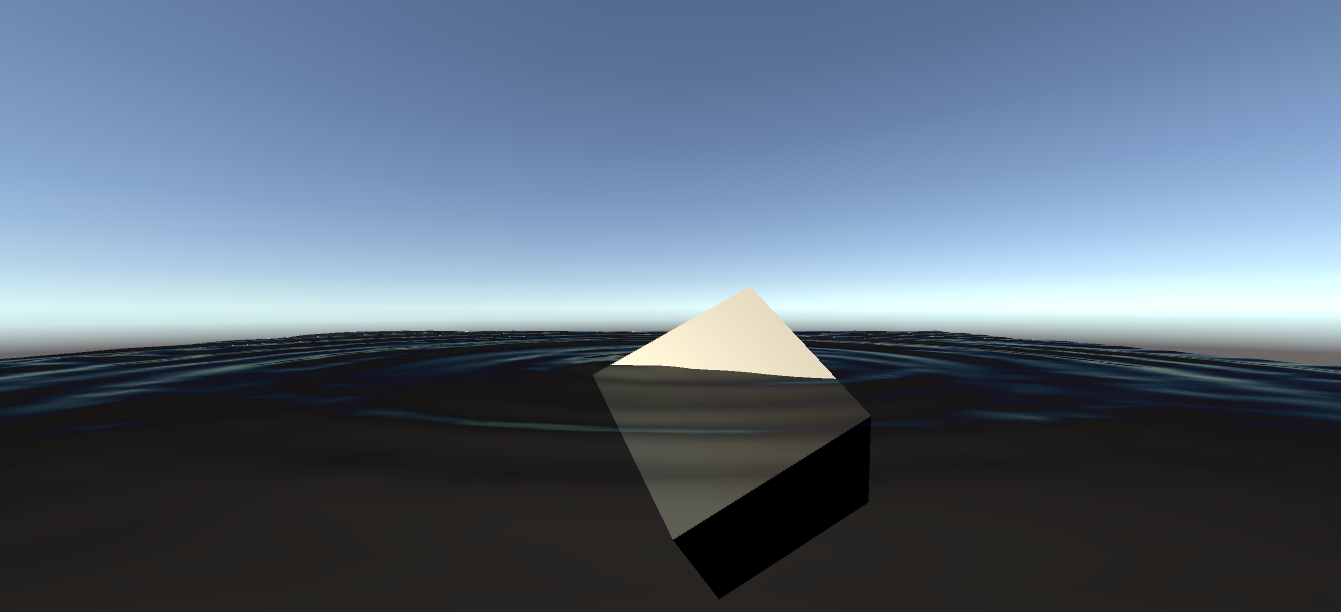
\includegraphics[width=\textwidth]{wave_particles_default_with_cube_1}
\caption{An example of water waves produced by a floating cube in my
implementation.}
\label{fig:wave_particles_example_snapshot}
\end{figure}

In this chapter, I introduce the terminology used in the dissertation
before covering the motivations for engaging in this project. Related work in
the field of fluid animation will then be covered, in addition to existing work
that has been done in industry using Wave Particles.

\section{Terminology}

\begin{itemize}

  \item \textbf{Frame-Rate:} The rate at which consecutive images (frames) are
  rendered by a graphics system.

  \item \textbf{(Soft) Real-Time Graphics:} Real-time programs have strict
  timing-based functionality requirements. With graphics, the goal is to
  produce frames in real-time. Hard real-time systems must meet their timing
  requirements in order to be considered functional, with soft real-time
  systems it is a goal \cite{gameenginebook}.

  \item \textbf{Game Engine:} A Game Engine is a software framework designed to
  facilitate the running and creation of a video-game.

  \item \textbf{Height-Field:} Given a surface, a height-field is a function
  from each $(x, y)$-point on that surface to some scalar height-value $z$.
  This function can then be used to distort the surface by displacing all
  points by that function in the vertical direction (in local space).

  \item \textbf{Extended Height-Field / Displacement Map:} These terms, used
  interchangeably, both refer to extending the concept of a height-field by
  making the output of its function three-dimensional. Therefore, points on a
  plane can be displaced both horizontally and vertically.

  \item \textbf{Trochoidal Wave:} A wave that has both longitudinal and
  transverse components. A full description is provided in Section
  \ref{sec:wave_particle}.

  \item \textbf{Wave Particle:} A particle on the surface of a body of water
  encoding a small section of a water-wave. See Section
  \ref{sec:wave_particle}.

  \item \textbf{Wave Particle System:} A water-wave animation system that uses
  Wave Particles. See Section \ref{sec:wave_particle}.

  \item \textbf{GPU:} Short for \textbf{Graphics Processing Unit}, the GPU is a
  piece of hardware designed for graphics rendering and imaging processing.
  % Most modern PCs and mobile systems have a GPU.

  \item \textbf{GPGPU:} Short for \textbf{General-purpose computing on graphics
  processing units}, is the use of GPUs for general-purpose computing. This is
  becoming increasingly common as GPUs are well-equipped for massively parallel
  computation.

  \item \textbf{VRAM:} Short for \textbf{Video Random Access Memory}, this is
  is the main pool memory that GPUs have access to. It is usually distinct from
  RAM used by the CPU, and connected to it via a bus. However, some modern
  architectures do have a unified pool of memory shared by the CPU and GPU
  \cite{AMDHuma}.

  \item \textbf{Triangle:} GPUs are optimised for a specific form of
  three-dimensional graphics rendering where objects and models are formed of
  many triangles.

  \item \textbf{Vertex:} A vertex in three-dimensional graphics is the vertex
  of one or more polygons (such as triangles).

  \item \textbf{Texture:} A texture is a one-, two-, or three-dimensional array
  of pixels stored in graphics memory.

  \item \textbf{Shader:} A shader is a piece of code that runs on the GPU. There
  are different types of shaders with different purposes.

  \item \textbf{\texttt{ComputeBuffer}:} An array-like buffer stored on the GPU.

\end{itemize}

\section{Motivation}

% OLD
% My motivation will cover why there is a demand for water simulation in
% real-time applications and the available options for simulating water. The
% limitations of existing systems will be shown - including how three-dimensional
% techniques are too computationally complex for real-time graphics and how most
% two-dimensional techniques are only able to simulate one-way interactions. This
% will lead into why the decision was made to implement the Wave Particles method
% as a real-time water simulation technique.

Simulating water in (soft) real-time (meaning a bare minimum operating speed of 30
frames per second \cite{gameenginebook}), continues to be a
big challenge, consistently being used as a benchmark for the current state of
real-time graphics \cite{gamingmobydick}. With the emergence of both Virtual and
Augmented Reality, the applications of complex real-time computer graphics are
increasing \cite{ARApplications} \cite{VRGrowth}.

% Section \ref{sec:related_work} explores existing water simulation techniques in
% detail, showing how they ultimately come in two flavours - full
% three-dimensional simulations that aim to capture in detail how water flows,
% and two-dimensional surface simulations that aim to simulate waves.

% OLD
% Three-dimensional systems can be unstable and complex for artists to use, which
% while suitable for offline renders such as films - only a single, deliberate
% 'take' of a particular scene is required - is completely out of the question in
% games as stability must hold-up over the course of hours of user interaction.
% Furthermore, they are computational expensive, and although are now possible to
% simulate in real-time, still use a lot of resources which could be spent on
% other systems in a Game Engine - as enemies, environments, post-processing
% effects, objects and even networking

% Two-dimensional systems can be accurate, convincing and cheap enough for
% real-time applications: many simply need to provide an entertaining and fun
% experience to a user on consumer-level hardware such as a PC, games console or
% even a smartphone. As discussed in Section \ref{sec:related_height_map}, a
% plethora of techniques have developed which aim to simulate the generation and
% interactions of water surface-waves on a two-dimensional plane - massively
% reduce the level of computation required, at the expense of not being able to
% accurately simulate splashes, vortices and other effects only a fully-realised
% 3D simulation could provide \cite{GPUGems}.

Wave Particles are a two-dimensional technique proposed by Yuksel at al. that
capture how wavefronts form and propagate by representing them with particles
\cite{Yuksel2007}. Incredibly large numbers of Wave Particles can be active, as
only a fraction of them need to be updated every frame - which is done in order
to subdivide them so that they can represent dispersing waves. They are a
simple idea that is well suited to the GPU; as each particle can be treated
independently. Furthermore, they are deterministic and allow for relatively
complex two-way fluid-object interactions. They have also been shown to be
incredibly flexible and exceptionally easy for artists to control
\cite{Tatarchuk:2016:ARR:2897826.2940291}. Finally, there is a lot of room for
them to be extended in a variety of ways (Section \ref{sec:future_extensions}).

My goal in implementing Wave Particles was to rebuild the system from the
ground-up in order to simulate surface-waves in real-time. Furthermore, I aimed
to analyse how well the system performed within a complex commercial game
engine - building the system in the Unity framework for this purpose. Finally,
I wanted to explore how they could be optimised by using GPU compute
shaders.

%POSSIBLE: summary

\section{Related Work}
\label{sec:related_work}

Here I give a broad overview of the field of Fluid Animation, how it relates to
Computational Fluid Dynamics, and its development in computer graphics, before
showing where wave simulation using displacement maps fits into the field.
Finally, I demonstrate existing work that has been done using Wave Particles.

\subsection{Fluid Animation}

% ENSURE: actual papers are mentioned as a lot of research was done!

Water simulation falls within the field of fluid simulation, which itself has two
overlapping sub-fields - that of fluid animation and computational fluid
dynamics. The former concerns itself solely with convincing visual effects
whereas the latter field is used to study the behaviour of fluids
scientifically. This dissertation concerns itself with fluid animation.

Fluid animation is itself a broad field, with most fluid animation systems
implementing some approximation or simplification of the Navier Stokes
equations \cite{NavierStokes} \cite{Stam:1999:SF:311535.311548}
\cite{Irving:2006:ESL:1179352.1141959}. The most comprehensive approach to
fluid animation is to implement a full three-dimensional simulation system.

% These come in two main flavours,
% Lagrangian and Eulerian.

% Lagrangian techniques use particles in a three-dimensional system to simulate
% fluid. Smoothed Particle Hydrodynamics (SPH) are such a technique introduced
% into computer graphics by Stam and Fiume in 1995 \cite{StamFiume1995}. SPH
% systems have been further extended and improved in various ways - enforcing
% incompressibility to model liquids and adaptive models that reduce the total
% number of particles required, whilst maintaining good quality simulations.

% Eulerian techniques are grid-based, offering a numerical solution to the Navier
% Stokes equations. A fluid is divided into cells in order to discretise it -
% first being introduced to computer graphics by Foster and Metaxas in 1996
% \cite{Foster:1996:RAL:244304.244315}. The stable fluids method introduced by
% Stam in 1999 used semi-Lagrangian advection to create a relatively efficient
% and unconditionally stable simulation using a Eulerian system
% \cite{Stam:1999:SF:311535.311548}.

% While powerful, these techniques have been traditionally limited to the domain
% of offline rendering: not being suitable for real-time rendering. Furthermore,
% many systems, such as Smoothed Particle Hydrodynamics can be unstable without
% sufficiently small time-steps \cite{SPH}, and have a host of other issues not
% making them suitable for real-time rendering.

% However,

Recent developments in General-purpose computing on graphics processing units
(GPGPU) and an increase in the power of GPUs have allowed real-time
three-dimensional particle-based fluid animation techniques to be developed,
including Position Based Fluids (PBF) by Macklin and M{\"u}ller in 2013
\cite{Macklin2013}. However, these are still intensive and limited to small
fluid-bodies. Additionally, any resources saved by implementing something more
simple can be used on other components of a real-time system (Physiscs, AI,
Graphical Effects, etc.).

With liquids such as water, a common simplification is to focus on animating
waves on the surface of a body. The reason for this is that doing so is
computationally simple, as the results of such a simplified simulation can be
rendered by displacing vertices in a mesh. This will be covered in the next
section.

\subsection{Wave Simulation \& Height-Fields}
\label{sec:related_height_map}

An explanation of height and displacement fields will be given, and how they
allow for very simple wave simulations. A few methods will then be described
which use these data-structures - including the sum-of-sines approach,
Gerstner Waves using Fast Fourier Transforms, Texture Shifting, and Wave
Particles.

A height-field is essentially a function of the form $z = f(x, y)$, mapping
points $(x, y)$ on a 2D plane to some height $z$. This formulation is
frequently used for water surfaces, as it is faster than 3D simulation methods,
however it is limited to vertical motion on a water surface. Furthermore,
height-field methods also incorrectly model water-waves, which are trochoidal
in nature - having both longitudinal and latitudinal components
\cite{Gerstner1802}.

Some of the limitations of height-field-based methods can be overcome with a
small extension - associating horizontal displacement to points on a 2D plane
in addition to the vertical one; more accurately called a displacement map.
This structure will also be referred to as an extended height-field - matching
the naming conventions in the original Wave Particles paper \cite{Yuksel2007}.
This structure is sufficient for most wave simulations, although it still can't
handle topological changes such as breaking waves.

Most two-dimensional systems are one-way. Meaning that ambient waves will be
simulated using artist-controlled variables and will physically exert forces on
floating objects, however objects themselves won't generate waves which have an
effect on the simulation. A common workaround to this is to pre-bake visual
effects, like splashes and ripples in order to create the illusion of a two-way
simulation system, even if the generated waves are purely visual \cite{RTR3}.
Figure \ref{fig:uncharted_no_wake} shows the results of the one-way system used
in \textit{Uncharted 4} (See Section \ref{sec:related_wave_particles}).

\begin{figure}[h]
\centering
\includegraphics[width=0.8\linewidth]{uncharted_no_wake}
\caption{A screenshot of \textit{Uncharted 4}, an example of a one-way
two-dimensional wave-simulation system. Although the boat generates white-foam
as a texture, no wakes are created \cite{Tatarchuk:2016:ARR:2897826.2940291}.}
\label{fig:uncharted_no_wake}
\end{figure}

A common technique for simulating turbulent oceans is the sum-of-sines
approach, where sine waves of multiples frequencies are used
\cite{GamaSutra3DWater}. This technique is slow, limiting the number of wave
frequencies that can be simultaneously computed. These can be supplemented with
texture shifting, a technique where multiple normal maps are tiled and layered
in order to imitate small ambient waves - a technique that can suffer from
visible patterns forming, destroying the illusion of ambient waves \cite{RTR3}.

Gerstner waves are an efficient one-way method for ocean simulation that use
Fast Fourier Transforms, enabling tens of thousands of waves at once
\cite{Tessendorf2001} \cite{GPUGems}. However, FFT-based systems are hard for
artists to control, something which is important
\cite{Tatarchuk:2016:ARR:2897826.2940291}. An implementation of this technique
can be seen in Figure \ref{fig:gerstner_example}.

\begin{figure}[h]
\centering
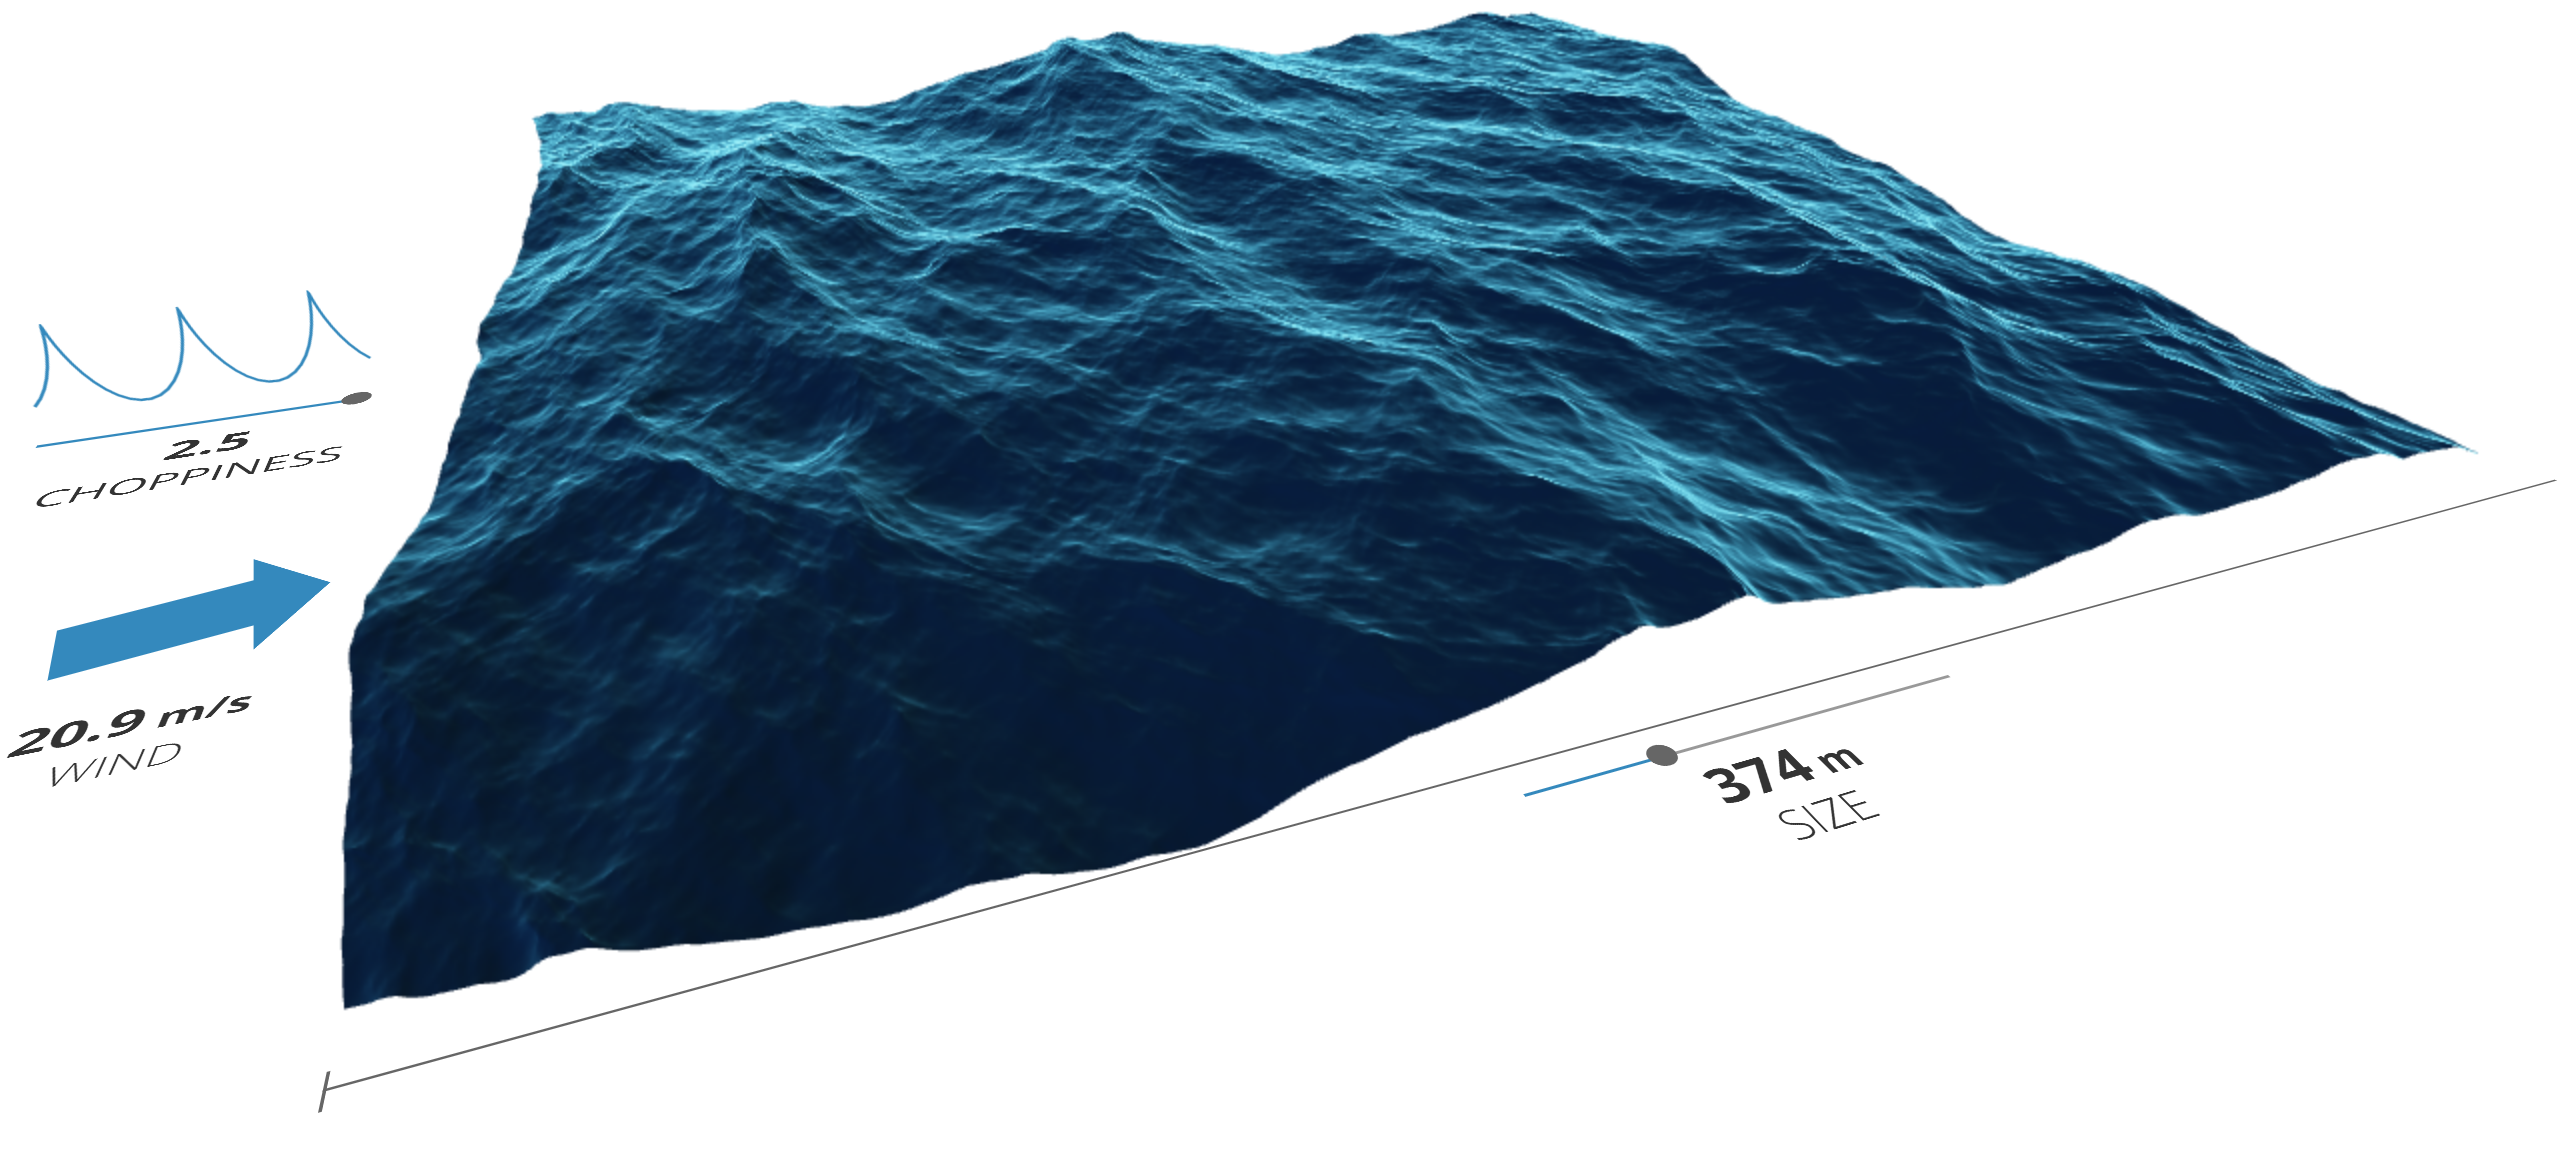
\includegraphics[width=0.8\linewidth]{gerstner_example}
\caption{WebGL rendering of Gerstner using Fast Fourier Transforms
\cite{DavidLiFFT}.}
\label{fig:gerstner_example}
\end{figure}

The last height-field based technique is Wave Particles, which can be used to
implement both one-way (Section \ref{sec:related_wave_particles}) and true
two-way systems \cite{Yuksel2007}.

Some systems have been developed that combine both two and three-dimensional
techniques \cite{Irving:2006:ESL:1179352.1141959}. However, these have so far
only been used in offline rendering.

% This section gave a brief explanation of the height-field, showing how
% limitations allow for much faster wave simulations that fully three-dimensional
% systems. Common height-field-based techniques such as sum-of-sines,
% texture-shifting and Gerstner waves were explained - including how they are
% limited to one-way interactions. It was then stated that Wave Particles, the
% subject of this dissertation, overcame this limitation. Finally, hybrid systems
% using both two and three-dimensional techniques have been used in offline
% rendering.

\subsection{Wave Particles}
\label{sec:related_wave_particles}

Here existing commercial use of Wave Particles will be explored; particularly
\emph{Naughty Dog}'s simulation of turbulent oceans and rivers using one-way
Wave Particle systems.

\emph{Naughty Dog} used Wave Particle techniques in the games \emph{Uncharted
3} and \emph{4} \cite{Tatarchuk:2016:ARR:2897826.2940291}
\cite{OchoaAndHolder2012}. Rather then being used to create convincing
fluid-object interactions alongside convincing wave generation; they were
employed to generate noise on-top of a Gerstner Wave-based ocean simulation
\cite{Tessendorf2001}. This was done by layering Wave Particle systems of
different amplitudes and frequencies - creating a system resembling turbulent
water.

\textit{Uncharted 4}, extended this technique from oceans to rivers by
advecting the animation in the direction of water-flow generated from an
offline 3D simulation.

These novel uses of Wave Particles lack one of its benefits - of providing
cheap two-way fluid-object interactions, rather than one way fluid-to-object
systems.

\subsection{Summary}

I gave an overview of the techniques used in Fluid Animation, including
three-dimensional systems. I introduced Position Based Fluids - a real-time
three-dimensional fluid simulation that can run on the GPU. I then explained
the limitations of these techniques and how their complexity still makes them
unsuitable for large real-time applications. Height field-based techniques
frequently used in games were then introduced. Finally, I showed where Wave
Particles are placed in the field, and existing work that has been done using
them.

\chapter{Preparation}

This chapter covers how I understood the mathematics behind Wave Particles,
from generating waves on a surface at a given time $t$, to how
plausible-looking fluid-object interactions occur within the system. I will
also cover the approach taken to rendering.

Secondly, I explain the approach taken to tackling the project from a
software engineering perspective: my starting point, the software I used and
finally the principles I applied in day-to-day development.

% ENSURE: DESCRIBE WORK UNDERTAKEN BEFORE CODE WAS WRITTEN

% ENSURE: SHOW HOW PROJECT PROPOSAL WAS REFINED AND CLARIFIED, SO THAT
% IMPLEMENTATION STAGE WENT SMOOTHLY

% ENSURE: CITE NEW PROGRAMMING LANGUAGES (C\#, HLSL), AND SYSTEMS WHICH HAD TO BE
% LEARNT AND MENTION COMPLICATED THEORIES AND ALGORITHMS WHICH REQUIRED
% UNDERSTANDING

\section{The Mathematics behind Wave Particles}

Here I cover the mathematics behind Wave Particles, defining a Wave Particle
and how it approximates waves on a water surface. Then I discuss the nature of
water waves, before progressing to how the distortion to the surface can be
calculated. Finally, I explain how subdivision works and discuss material
appearance.

\subsection{The Wave Particle}

\label{sec:wave_particle}

I give an outline of the Wave Particle, its representation on a surface, and
how a displacement map is obtained at time $t$. Each component of the Wave
Particle is further explained and explored, covering its starting time $t_0$,
velocity $\bm{v}$, amplitude $a$, radius $r$, origin $\bm{o}$, and dispersion
angle $\theta$.

Within a Wave Particle system, each particle represents a moving unit of
distortion on a surface - contiguous wavefronts being represented by an arc of
particles where each are within $r/2$ of each other. In order to prevent
expanding wavefronts from fragmenting as constituent particles separate, each
Wave Particle stores both the origin $\bm{o}$ and dispersion angle $\theta$ of
the wave section it constitutes. A Wave Particle will subdivide based on this,
its radius $r$, and its velocity, such that the overall wavefront does not
become discontinuous. This emulates waves on the surface of a liquid in both
appearance and behaviour, satisfying the two-dimensional wave equation
(Equation \ref{eq:wave}) \cite{Yuksel2007}.

\begin{equation}\label{eq:wave}\frac{\partial ^2 z}{\partial x^2} + \frac{\partial ^2
z}{\partial y^2} = \frac{1}{v^2} \frac{\partial ^2 z}{\partial t^2 }
\end{equation}

Here $x$, $y$, and $z$, represent motion in the $x$-, $y$-, and $z$-axes
respectively, with $z$ being the vertical axis. $v$ is the speed of a wave,
while $t$ represents time.

The displacement map of surface-waves created by Wave Particles at time $t$ is
obtained from the superposition of all particles at time $t$ in the system.

\subsubsection{Water Surface-Waves}

Water surface-waves are trochoidal in nature - having longitudinal and
latitudinal components. This result comes from an exact solution of the Euler
equations for periodic surface gravity waves \cite{Gerstner1802}. These
equations are a particular form of the Navier-Stokes equations for fluids.
Gerstner waves describe progressive surface waves of an incompressible fluid of
infinite depth \cite{Gerstner1802}. Thus the trajectories of points on a
water-surface will be that of a closed circle - important in emulating the
appearance of water.

% TODO: add figure of the closed-circle movement of a Wave Particle
% https://commons.wikimedia.org/wiki/File:Trochoidal_wave.svg

% Equations \ref{eq:trochoidal_x} and \ref{eq:trochoidal_y} both describe the
% longitudinal and latitudinal components of trochoidal waves respectively.

% \begin{equation}\label{eq:trochoidal_x}X(a,b,t)=a+\frac{e^{kb}}{k}sin{(k(a+ct))}\end{equation}

% \begin{equation}\label{eq:trochoidal_y}Y(a,b,t)=b-\frac{e^{kb}}{k}cos{(k(a+ct))}\end{equation}
% % TODO(Rafal): explain symbols

\subsection{Calculating Distortion}

I explain the nature of water surface-waves and how the distortion that
each Wave Particle generates can be calculated such as to match these waves.

Given a Wave Particle at position $(x_p, y_p)$, of amplitude $a_p$, and with
radius $r$, the displacement it causes at any position $(x, y)$ on a plane can
be calculated using Equation \ref{eq:particle_distortion},

% POSSIBLY: Look into splitting equations

\begin{equation} \label{eq:particle_distortion}
\begin{split}
\bm{X}_p(x,y)=a_p(\gamma-B\sin{(\gamma)})\frac{(x_p-x,y_p-y)}{||(x_p-x,y_p-y)||}\rect(\frac{||(x_p-x,y_p-y)||}{r}) \\
Y_p(x,y)=\frac{a_p}{2}(\cos{(\gamma)} + 1)\rect(\frac{||(x_p-x,y_p-y)||}{r})
\end{split}
\end{equation}

where $\gamma=\sqrt{(r-(x-x_p))^2+(r-(y-y_p))^2}$ and rectangle function
$\rect(x)$ is $1$ for $|x| < 1$, $\frac{1}{2}$ for $|x|=1$, and $0$ otherwise.
$Y_p$ gives the transverse component, whilst $\bm{X}_p$ describes the
longitudinal component - giving the trochoidal effect
\cite{Tatarchuk:2016:ARR:2897826.2940291}. $B$ is a parameter ranging from $0$
to $1$ used to adjust the \textit{peakiness} of a Wave Particle (Figure
\ref{fig:distortion_diagram}).

\begin{figure}[h]
\def\svgwidth{\linewidth}
\input{images/wave_particle_side_on.pdf_tex}
\caption{Diagram showing the distortion caused by single Wave Particle at time
$t$. The particle starting at position $p$, travels a distance $d$, at
velocity $\bm{v}$, for time $t$. It has amplitude $a$ and radius $r$.}
\label{fig:distortion_diagram}
\end{figure}
% TODO(Rafal): plot this graph in matplotlib?

To calculate the displacement caused by all Wave Particles in the system at any
point on the plane, we take the sum of all particles (Equation
\ref{eq:particle_distortion_sum})

\begin{equation} \label{eq:particle_distortion_sum}
\begin{split}
\bm{X}(x,y) & =\sum_{p}\bm{X}_p(x,y) \\
Y(x,y) & =\sum_{p}Y_p(x,y)
\end{split}
\end{equation}

$\bm{X}$ and $Y$ describe the total longitudinal and transverse displacement at
any point on the plane respectively.

\subsection{Subdivision}

\label{sec:subdivision}

I explain how subdivision allows Wave Particles to represent a contiguous
dispersing wavefront with a given origin and angle.

Wave Particles in any arbitrary arc, where each particle is within $r/2$ from
the next, form a contiguous wavefront satisfying the Wave Equation (Equation
\ref{eq:wave}) \cite{Yuksel2007}. Therefore a dispersing wavefront composed of
such a system of particles naturally decreases in amplitude and remains
contiguous until separation distances of the particles exceed $r/2$.

If the Wave Particles are able to independently subdivide at such a point, we
can represent such wavefronts for an arbitrary length of time and perform
subdivisions in parallel - important in efficiently implementing such a system.

To achieve this, each Wave Particle is given both an origin $\bm{o}$ and
dispersion angle $\theta$. Figure \ref{fig:subdivision_diagram} demonstrates
and explains how subdivision then works. It is important to note that when a
Wave Particle is created, the time at which it will subdivide can be
pre-computed.

\begin{figure}[h]
\def\svgwidth{\linewidth}
\input{images/wave_particle_subdivision.pdf_tex}
\caption{Diagram showing how a Wave Particle generated at a position $\bm{o}$
with dispersion angle $\theta = \pi$, amplitude $a$, and radius $r$ subdivides.
It subdivides (the orange arrows) once into three particles when it has
travelled by a distance $d$ such that $d\theta = r/2$. These new particles have
the same speed, origin and radius, but a third of the amplitude and dispersion
angle. When they have travelled a distance $d$ such that $3d\theta/3=r/2$, they
independently subdivide again. Blue dashed lines indicate the areas individual
particles sweep out. Therefore, no two particles can separated by more than
half their radii, maintaining a contiguous wavefront.}
\label{fig:subdivision_diagram}
\end{figure}

\section{Starting Point}

I had read various papers surrounding water and fluid simulation, but hadn't
yet revised all the mathematics that was involved in all of the systems.

I started with an empty Unity project and had to learn the framework. Therefore
I had to learn C\# which is fortunately similar to the more familiar Java
\cite{UnityScripts}.

Furthermore, whilst having theoretical understanding of the GPU, I was
unfamiliar with programming for one, having to learn \textit{HLSL}, the shading
language of Unity \cite{UnityShaders}.

I used the example dissertation to construct my own.

Finally, Huw Bowles, a professional graphics programmer, had given me advice on
which papers to read and which technologies to use, ensuring I started in the
right direction.

\section{Software Used}

Here I describe the software used in implementing and evaluating Wave Particles
- including why I decided to use the Unity game engine, which programming
languages I used, the development environment I worked in, and the tools I used
for profiling and debugging.

\subsection{Game Engine}

I justify why I chose the Unity game engine to achieve my goal of implementing
the project within one.

Unity is a versatile, scalable, and portable cross platform game engine used by
both independent developers and big publishers. Its ease-of-use means that
shader-programming is straight-forward. However, C\# being the most
commonly-used language in Unity means garbage-collection can cause performance
issues in real-time applications unless handled carefully
\cite{UnitySharpWins}. %POSSIBLE MOVE SENTENCE ABOVE

The ease of writing portable shaders with minimal set-up is the reason why I
settled on using Unity. This was extremely important I had to implement Wave
Particles on the GPU. Furthermore, my inexperience of writing shaders before
embarking on the project made it important to pick a solution providing minimal
friction, so the focus could be on implementation as opposed to set-up and
boilerplate.

Although garbage-collection is an issue in Unity, Section
\ref{sec:evaluation_memory} describes how this can minimised as memory tends to
be fixed and limited in real-time graphics. Unfortunately, multi-threading
support is still limited in Unity \cite{UnityBadThreading}.

\subsection{Programming Languages}

Here I cover C\#, HLSL and Python, programming languages I used on the project.

\textbf{C\#:} Unity offers the ability to program in a custom variant of
JavaScript (called UnityScript) or C\# \cite{UnityScripts}. I settled on C\# as
it is the most supported and documented of the two \cite{UnitySharpWins}. C\#
is similar to C++ and Java.

\textbf{HLSL:} HLSL is a shader language developed by Microsoft. Shader
languages are programs that run on the GPU. Unity can automatically
cross-compile HLSL programs to different platforms, therefore, using it is
encouraged \cite{UnityShaders}.

\textbf{Python:} Python was used in evaluation. I was familiar with the
language and knew that powerful libraries existed for numerical analysis. I
learnt \textit{NumPy}, \textit{pandas}, and \textit{Matplotlib} so I could
process my data and generate graphs \cite{NumPy} \cite{pandas}
\cite{Matplotlib}.

\subsection{Development Environment}

This section gives an overview of Git, Travis CI and Visual Studio, the tools
featuring in my development environment.

\textbf{Git \& GitHub:} Using Git as version control was the first thing I
setup, due to its importance and ease-of-use. Furthermore, I committed all
documents and software to version control immediately upon creating their
stubs.

I used branching and tags to improve productivity, as they allowed for me to
context-switch between completing different features and keep track of
particularly notable parts of the project for this dissertation.

GitHub was used to provide a back-up of the project repository that served to
keep the project in sync between different platforms.

\textbf{Unit Testing \& Travis CI:} Unit testing is a good way to sanity-check
assumptions being made, help ensure changes made are non-breaking, and assist
in planning the interfaces of systems.

Unity provides a built-in unit tester that can hook into the engine
\cite{UnityEditorTestRunner}. However, Travis CI, an online system for
automatically running unit tests GitHub, does not provide native support for
Unity or even Windows \cite{TravisCILanguages} \cite{TravisCIOS}.

I wrote a script that automatically downloads the OSX version of Unity and
installs it onto a Travis CI OSX instance, running the Unit Tests from there.
The code I used for this is given in Appendix \ref{app:travisci}.

\textbf{Visual Studio:} Visual Studio was used because it is well supported,
integrates well with Unity and is the most common IDE used in the games
industry \cite{UnityVisualStudio} \cite{gameenginebook}.

\subsection{Profiling and Debugging Tools}

Profiling is extremely important when developing performance critical
applications. With many modern games, the 90-10 rule applies: 10\% of the code
runs 90\% of the time \cite{gameenginebook}. This means that optimising that
10\% is extremely important - profiling can be used help identify and optimise
that code in an evidence-based manner. Finally, profiling was used as part of
the evaluation.

\subsubsection{Unity}

Unity has a powerful integrated profiler, shown in Figure \ref{fig:profiler}.
It provides a variety of features, including the ability profile arbitrary
segments of code, memory allocations, number of calls, running time, graphics
memory allocations, and GPU usage.

I used the MIT licensed \textit{Unity Profiler Data Exporter} to export
profiling data to the JSON format so that it could be analysed in Python
\cite{UnityProfilerDataExporter}. This was done as Unity does not provide any
native functionality for exporting profiling data.

\begin{figure}[h]
\centering
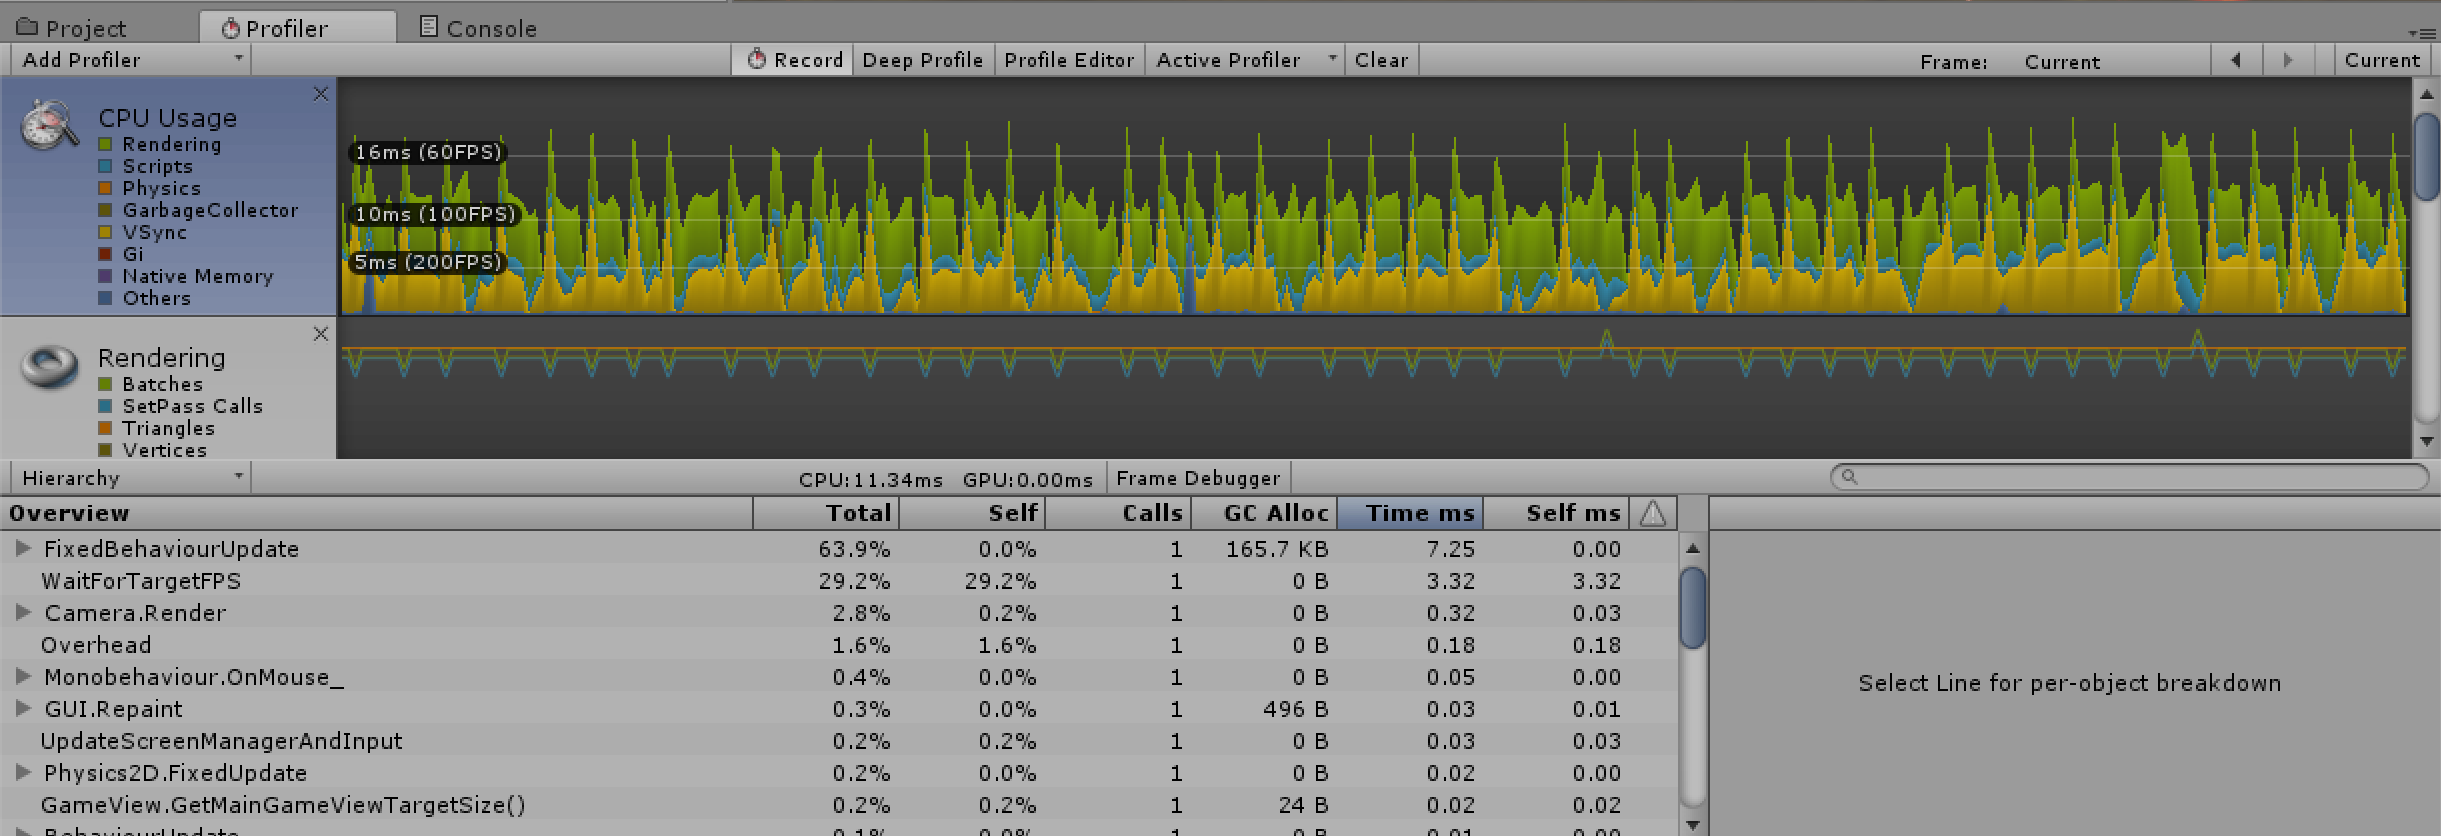
\includegraphics[width=0.8\linewidth]{profiler}
\caption{A screen-shot of Unity's profiler. Various provided features can be
seen here, including the ability to drill down to functions, what percentage of
each frame they take, their run time, and their memory allocations.}
\label{fig:profiler}
\end{figure}

\subsubsection{RenderDoc}

RenderDoc (Figure \ref{fig:renderdoc}) is a graphics profiling tool I used in
debugging and image exporting, as it allows users to analyse the state of the
graphics pipeline \cite{RenderDoc}.

\begin{figure}[h]
\centering
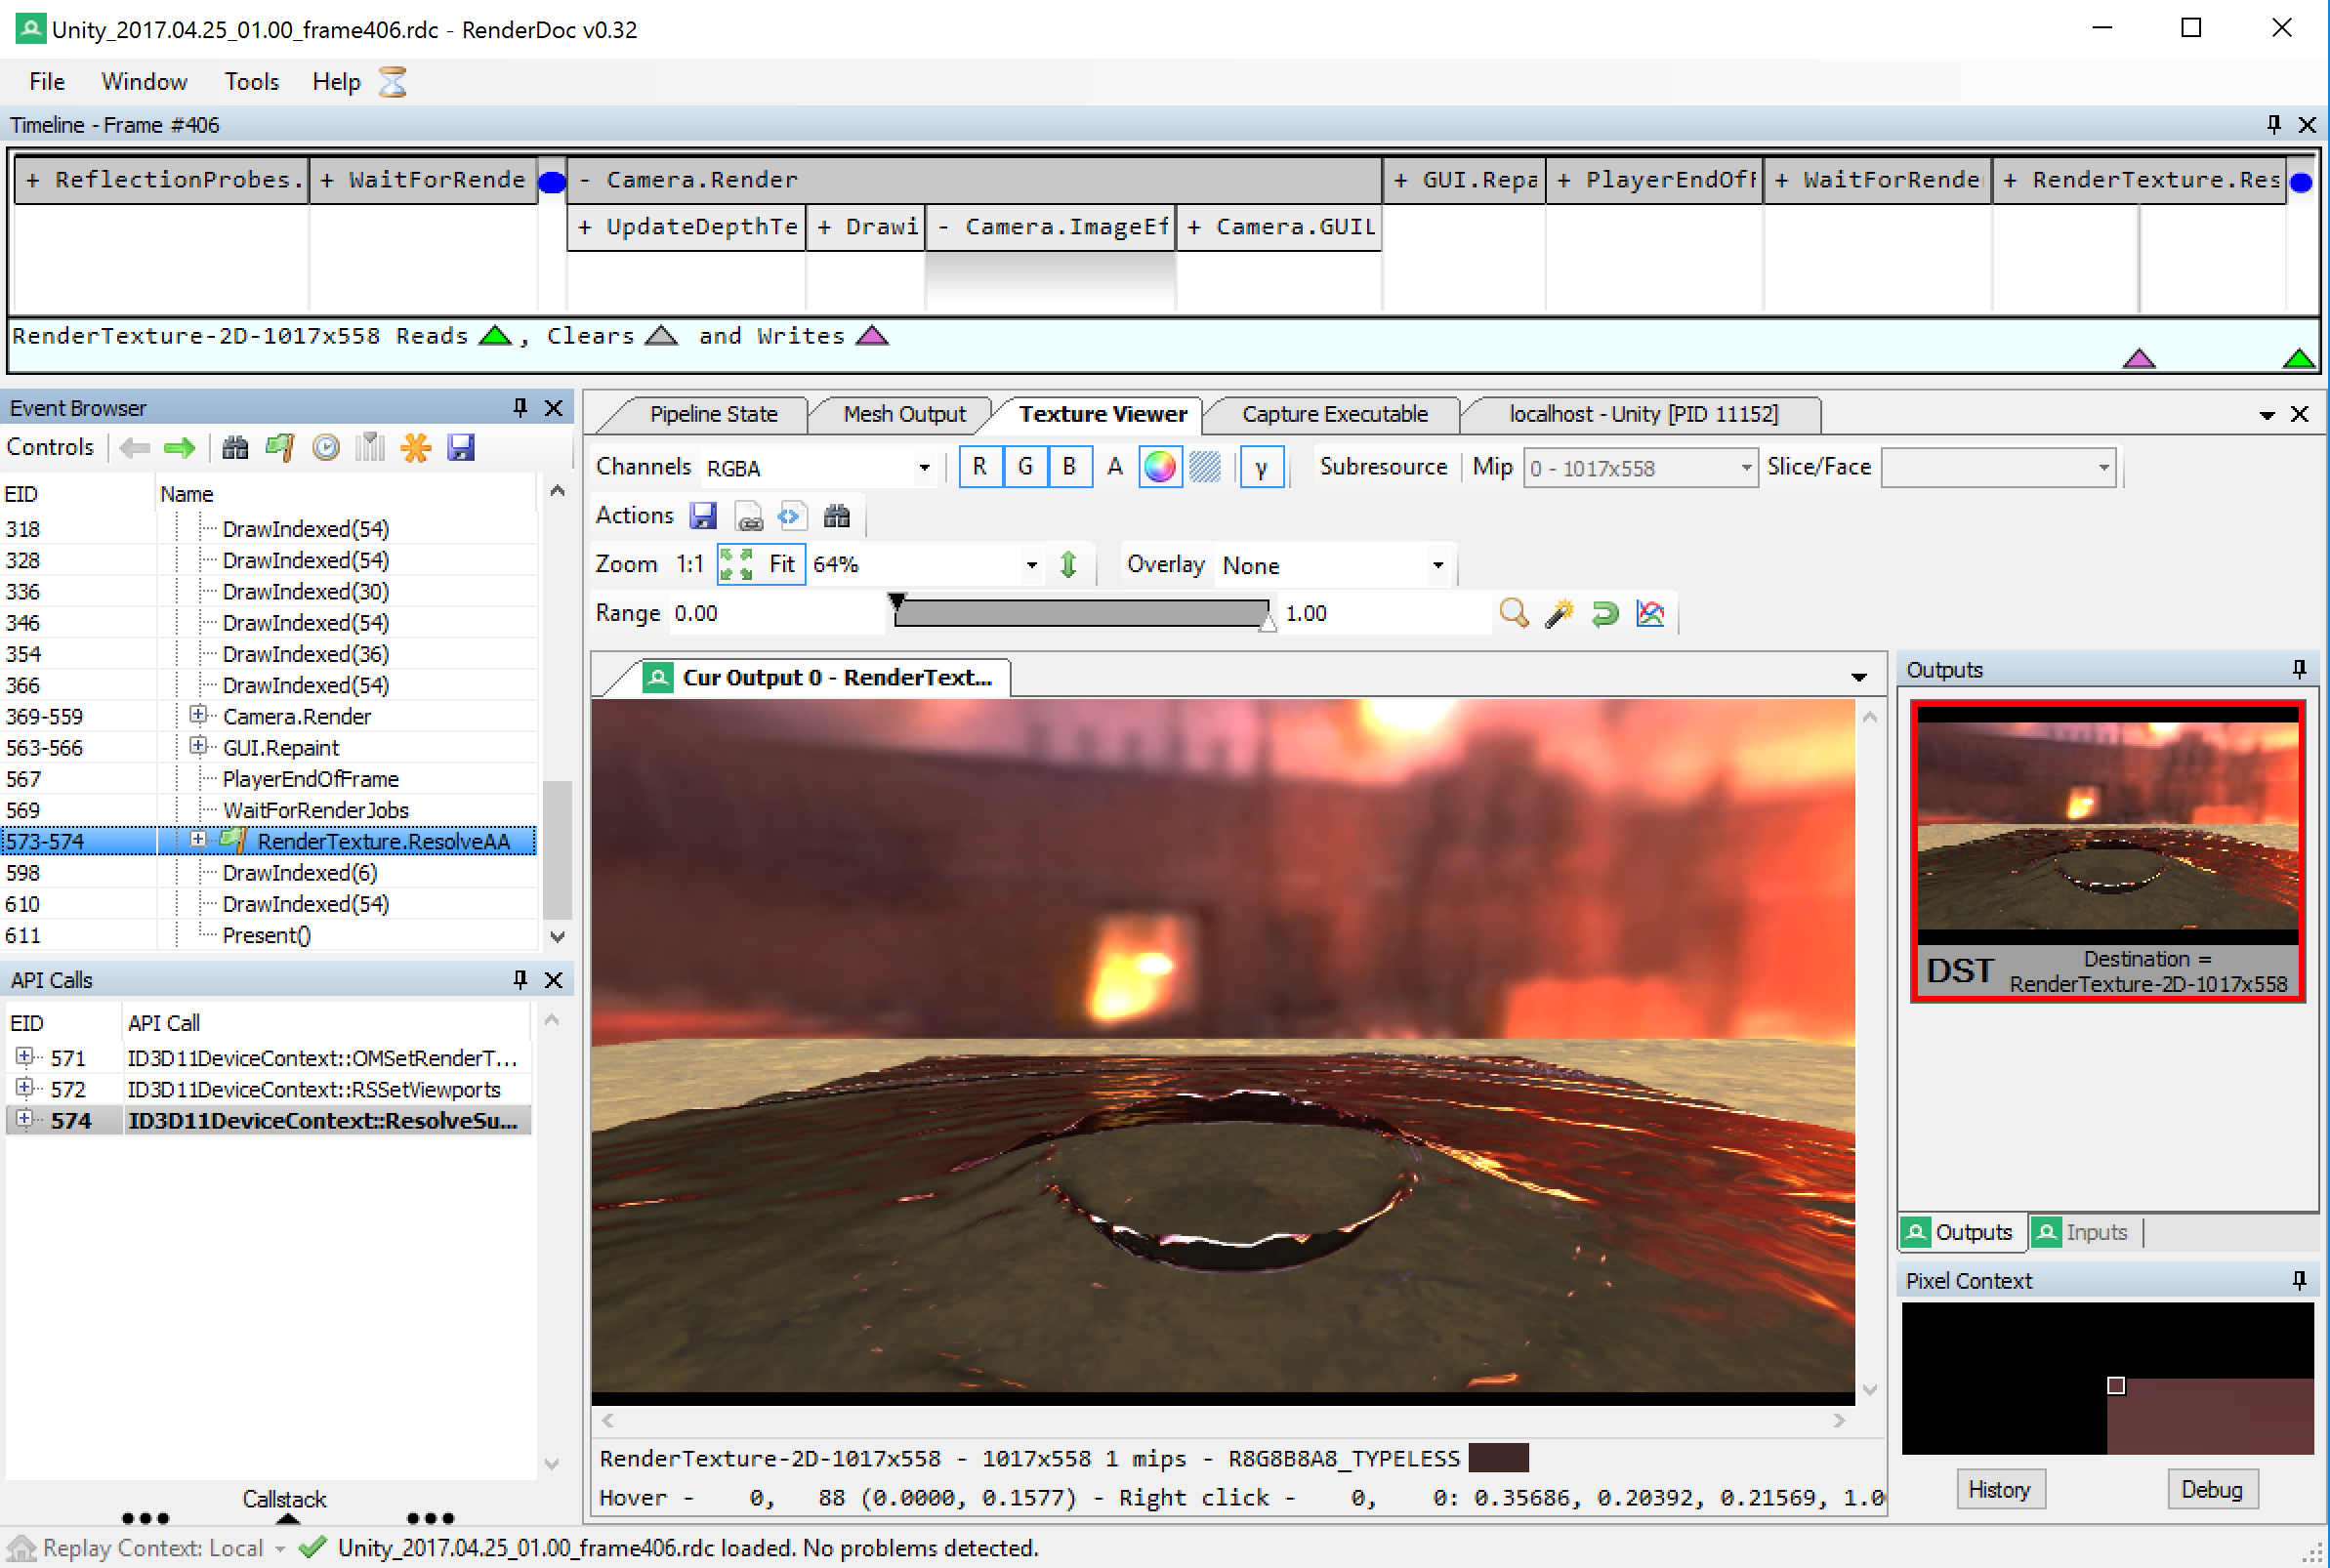
\includegraphics[width=0.8\linewidth]{renderdoc}
\caption{Screen-shot of RenderDoc running on the project.}
\label{fig:renderdoc}
\end{figure}


\section{Software Engineering Principles}

% ENSURE: CHANGES TO STARTING POINT DIFFERENT FROM PROJECT PROPOSAL ARE EXPLAINED

% POSSIBLE: READ OTHER STARTING POINTS FOR TYPICAL CHANGES/TENSE

% ENSURE: PROFFESIONAL APPROACH WAS EMPLOYED

% ENSURE: IT HAS THE QUALITIES REQUIRED TO MAKE A GOOD PREPERATION chapter (BASED
% ON OTHER PROJECTS I HAVE READ)

% ENSURE: IT CONTAINS A subsection HEADED "Requirements Analysis" AND INCORPORATES
% OTHER REFERENCES TO THE TECHNIQUES OF SOFTWARE ENGINEERING.

%TODO: Write section introduction

The Wave Particles system is a pipeline of stages that runs once per frame,
described in the Section \ref{sec:implementation_pipeline}. As there are many
different strategies for implementing each stage, I ensured they each had a
well-defined interface allowing for different possible implementations.

\subsection{Software Development Model}

As so much was unknown going into the project, having a reliable software
development model was a priority. Firstly, I prototyped a two-dimensional
version of Wave Particles in a simple two-dimensional engine called GameMaker
so ideas could be tested (Figure \ref{fig:wave_particles_prototype})
\cite{GameMakerStudio}. I then designed the pipeline using the
\textit{waterfall model}, such that each component could then be independently
designed, implemented and analysed using the \textit{spiral model}
\cite{WaterfallModel} \cite{SpiralModel}. Achieving visual results early was
important, therefore I decided to focus on the visual stage first -
implementing stubs for all the other parts. This was done by designing and
hard-coding a system with a single Wave Particle. From there, I iteratively
fleshed out the project with new features as my understanding of the project
and Unity grew.

\begin{figure}[h]
\centering
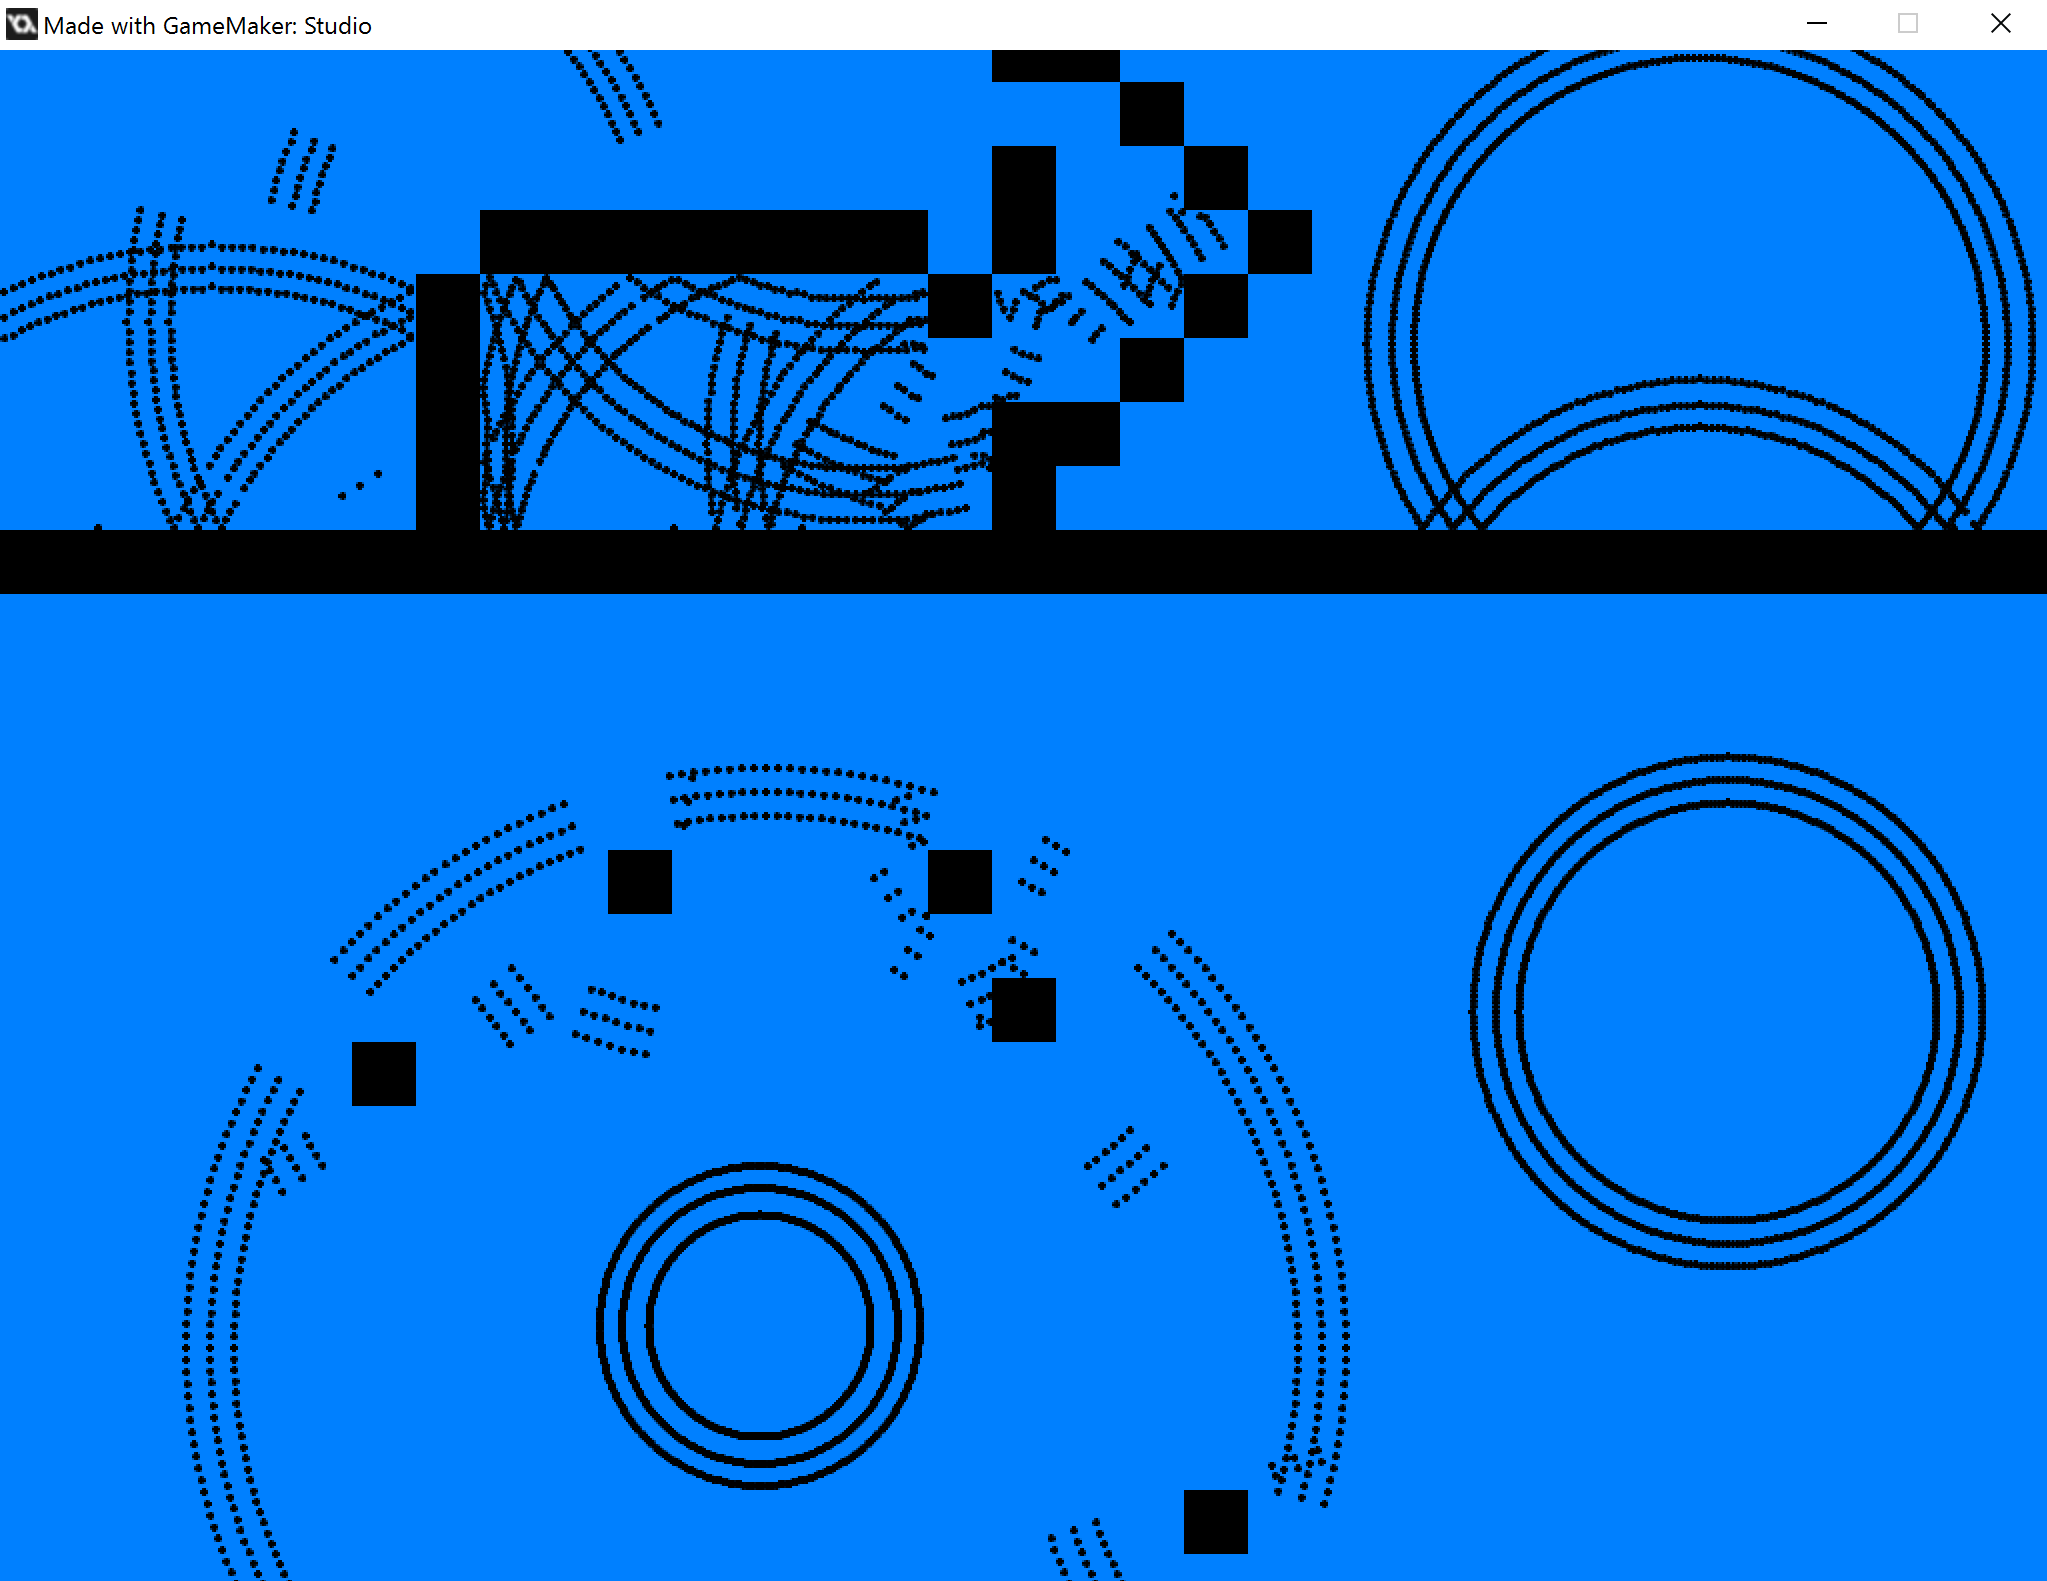
\includegraphics[width=0.8\textwidth]{wave_particles_prototype}
\caption{A Wave Particles prototype implemented in GameMaker Studio.}
\label{fig:wave_particles_prototype}
\end{figure}

\subsection{Requirements Analysis}

I used the \textit{MoSCoW} method in order to prioritize the requirements and
extension ideas from the project proposal, labelling parts of the project
\textbf{Must have}, \textbf{Should have}, \textbf{Could have}, and
\textbf{Won't have} as listed below \cite{MoSCoWMethod}.

\subsubsection{Project Requirements}

\begin{itemize}

\item \textbf{Must have} a Wave Particle simulation in Unity that runs on both
the CPU and GPU with the ability to easily compare the performance of each.

\item \textbf{Must have} the complete GPU-based version of the simulation run
at least 30 frames-per-second with 5000 Wave Particles present.

\item \textbf{Must have} a 2D top-down overlay-visualiser of the wave-particles
to enable easy visualisation of what is going on, for both explanatory and
debugging purposes.

\item \textbf{Must have} a basic water renderer for the wavefronts generated by
the Wave Particles.

\item \textbf{Must have} measurements comparing the performance of the CPU and
GPU based implementations of specific features, in addition to, data of how the
number of Wave Particles affect the performance of the simulation alongside the
resulting visual outcome.

\item \textbf{Should have} a system to manage the Wave Particles and object
placement within the Unity editor.

\item \textbf{Should have} A fluid-object interaction system on both the CPU
and GPU with the same criteria as above.

\end{itemize}

\subsubsection{Extensions}

\begin{itemize}

\item \textbf{Could have} more realistic water shaders for rendering the water,
measuring how they affect the performance of the simulation in addition to how
they compare to the real physical phenomena they represent.

\item \textbf{Could have} the ability to view the scene in virtual-reality.
Importantly, this requires running at a framerate of at least 90 frames per
second to help prevent motion sickness that can be exacerbated by lower
framerates.

\item \textbf{Won't have} the ability to handle the degenerate cases where
splashes should occur using a simplified Smoothed Particle Hydrodynamics-like
simulation.

\end{itemize}

\section{Summary}

This chapter discussed the initial research I did and the mathematics behind
the Wave Particles system. Furthermore, I described the fundamental features I
used to implement the project. Finally, I demonstrated the tools and
development environment I used in creating the project, in addition to the
software engineering principles I employed such as the \textit{MoSCoW} method.

\chapter{Implementation}

% ENSURE: WHAT WAS PRODUCED IS DESCRIBED (THE PROGRAMS THAT HAVE BEEN WRITTEN)

% ENSURE: DESIGN STRATEGIES THAT LOOKED AHEAD TO THE TESTING STAGE

Here I discuss how I implemented the Wave Particles system. I first explain
some of the key insights that can be derived from theory which enable an
efficient implementation. I then describe the concrete data-structures that I
created - including the Wave Particles pipepline. Following that, I delve into
the details of how I implemented different parts of the system, including
subdivision, Wave Particle reflections, displacement map generation,
fluid-object interactions, rendering, and novel techniques I developed to
improve performance. Finally, I discuss how I performed profiling and
optimisation before summarising the chapter.

\section{Insights}

Here I describe the insights that allow the Wave Particle
system to be implemented in software - specifically how the theory developed
into implementation. I start by describing the system from an algorithmic
point of view, including approximations and assumptions that can be made in
order to enable key optimisations and expose parallelisation opportunities in
subdivision. Finally, I describe how convolution can be used to
efficiently generate the displacement map.

\subsection{Computing Subdivisions and Reflections}

One insight that allows the Wave Particles system to comfortably run at
real-time frame rates, is that once generated, a Wave Particle is never
modified except on subdivision and reflection with static obstructions.
Furthermore, the frame in which a Wave Particle will need to be
subdivided/reflected can be calculated at the time it is generated. This means
that for any given frame, we know the set of Wave Particles that need to be
iterated over for these operations. The result of this, is that even in a
system with many thousands of Wave Particles, only a fraction need to be
updated, however, iteration over all of them is still required when generating
the displacement field.

\subsection{Obtaining the Displacement Map Using Convolution}
\label{sec:implementation_overview_obtain_displacement_map}

This section will cover how I used convolution to calculate the displacement
map generated by a system of Wave Particles \cite{Yuksel2007}.

In software, I used a two-dimensional image mapped to the water's surface to
encode the displacement map - each pixel encoded the displacement at that point
on the water's surface. Convolution can be used to efficiently calculate the
desired displacement map given a system of Wave Particles, if we assume each
has a fixed and shared radius, $r$.

The naive approach to calculating the displacement map would be, for every
pixel, to iterate through every Wave Particle in the system and calculate its
total contribution to the displacement at that pixel - a direct implementation
of Equation \ref{eq:particle_distortion_sum}. Pseudocode for this is show
below.

\begin{lstlisting}
for each pixel
    for each wave_particle
        pixel += calculate_distortion(wave_particle)
    end
end
\end{lstlisting}

However, given that each Wave Particle has the same radius, the distortion each
generates has the same form - simply with different amplitudes, which can be
encoded in a two-dimensional filter kernel. Therefore, I generated the final
displacement map by \textit{splatting} the amplitude of each Wave Particle to
an image of an identical resolution to the displacement map. By convolving this
image with a Wave Particle kernel, I could efficiently compute the displacement
map, encoding the total distortion caused by all the Wave Particles in a given
system. Figure \ref{fig:convolution_2D_example} shows the result of convolving
the Wave Particle kernel with a splatted image. This gives the same result as
Equation \ref{eq:particle_distortion_sum} at a lower computational cost
\cite{Yuksel2007}.

\begin{figure}[h]
\centering

\includegraphics[width=0.1\linewidth]{convolution_2D_kernel}
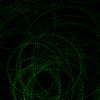
\includegraphics[width=0.4\linewidth]{splat_texture}
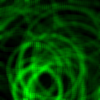
\includegraphics[width=0.4\linewidth]{displacement_map_texture}
\caption{The left-most image shows the convolution kernel generated from
Equation \ref{eq:particle_distortion}. The middle image shows the result of
splatting the amplitudes of a system of Wave Particles. The right-most image
shows the final displacement map: The result of convolving both with each
other.}
\label{fig:convolution_2D_example}
\end{figure}

Although the kernel is non-separable, Yuksel et al. describe a one-dimensional
approximation that my system doesn't implement \cite{Yuksel2007}.

% OLD

% \section{Design Strategies}

% This section describes some of the design decisions made for this project.
% Including how I prepared for evaluation and used Unity.

% \subsection{Preparing for Evaluation}

% One of the main goals of the project was to be able to easily compare the
% performance of specific features and implementations of those across both the
% GPU and CPU, the design of the project had to take this into account. In order
% for this to be achieved, the following criteria would have to be met:

% \begin{itemize}

%  \item  Easy, consistent profiling that can be done on a granular level

%  \item The ability to easily switch between implementation strategies for
%  components of the system (possibly even at runtime)

% \end{itemize}

% The latter was especially important to get running as early as possible, as it
% enabled me to easily compare earlier, naive implementations of the Wave
% Particles system I created and compare them with optimisations that were
% constructed as the project continued.

% \subsection{Using Unity}

% Ensuring the Wave Particles system was not only implemented, but also heavily
% integrated into the Unity SDK and game engine was vital. Not only because doing
% so gave the Wave Particle system access to the powerful pre-existing libraries
% and tools Unity provides, but also because it can expose parts of the system
% which may need to be adapted to make it suitable in a more fully-featured
% whole.

% However, care was also needed to make sure the core implementation details and
% algorithms were as decoupled from the rest of Unity as possible so that those
% components aren't dependant on the Unity environment. This helps ensure that the
% code is much easier to potentially port to other platforms and environments.

% OLD
% \section{Programming for the GPU}

% Programming for the GPU posed various challenges, both within the context of
% working with the Unity game engine and simply the task of maintaining, updating
% and designing code for it.

% This section describes the general issues faced, and opportunities provided by
% programming for the GPU. Information on how specific parts of the project were
% implemented on the GPU can be found in the sections describing those.

% \subsection{Memory}

% % POSSIBLE: add more references

% GPUs typically have a pool of memory that is both distinct and physically
% separate from the RAM - the pool of memory that a CPU has access to. (However,
% some devices are beginning to use a unified pool of memory, such as the PS4
% \cite{DFPS4}.) This pool of memory is referred to as VRAM. However, memory does
% need to be transferred back and forth from one pool to the other, with the
% limited bandwidth and latency of the bus used for this being a major bottleneck
% in a lot of game engines. Therefore, limiting the amount of memory transferred
% between the two is important, which is was a focus of many of the data
% structures used in my Wave Particles implementation.

\section{Data-Structures}

I first explain how every component of the Wave Particles system can be
implemented efficiently in software, giving the overall \textit{Wave Particles
Pipeline} that is executed in every time step. I then describe the novel
\texttt{ExtendedHeightField} class that I used to allow for the efficient
transfer of an image encoding the displacement map from one stage of the
pipeline to the next - across differing implementations.

I then cover how I implemented each step in the pipeline independently in
the following sections, explaining in detail how each part was implemented on
both the CPU and the GPU, and some of the novel data-structures I used to
optimise them.

\subsection{The Pipeline}
\label{sec:implementation_pipeline}

Here I describe the pipeline data-structure, a design I used in order
to encapsulate each part of the implementation.

I considered the Wave Particles system as a pipeline that runs every frame,
with the state of the Wave Particle system in the previous frame as the input.
The pipeline has multiple stages, each with a distinct purpose. I designed the
pipeline so that I could consider what interface each stage needed to provide -
it formed the framework of the entire project. A diagram of the pipeline is
given in Figure \ref{fig:pipeline}, where each stage is described.

\begin{figure}[h]
\centering
\def\svgwidth{\linewidth}
\input{images/wave_particles_pipeline.pdf_tex}
\caption{A diagram of the Wave Particles pipeline. Although some stages may
implement different strategies, the pipeline is designed around what is shown.
The Wave Particles are first subdivided and then drawn as point-particles to a
two-dimensional image which is convolved with a kernel representing the
displacement function of individual particles. The generated displacement map
is then used to displace vertices on the water-surface to display the waves.
This data can then be used in fluid-object interactions.}
\label{fig:pipeline}
\end{figure}

I designed the pipeline to be responsible for transferring the inputs of one
stage to the next, so that each stage could focus on transforming and operating
on data, without convoluted management. This was done by using the strategy
pattern, where each stage is abstracted using a C\# interface
\cite{StrategyPattern}. This ensured that the interfaces of each stage were kept
clean, allowing me to create, test, and compare multiple implementations of
each one in isolation.

However, in order to allow this pipeline to be as efficient as possible, I had
to use a novel data-structure to encode image information that passes through
each stage in a manner that was efficient and simple to interface with. This is
described in Section \ref{sec:extended_height_field}.

\subsection{Displacement Map}
\label{sec:extended_height_field}

Here I explain how I designed a novel data-structure, named
\texttt{ExtendedHeightField}, to encode displacement map image data. I will
then explain my goal to avoid unnecessary copying from RAM to VRAM. The
state machine I used to achieve my goals is then described, before I finally
justify why I decided to have the data-structure expose its contents directly,
as opposed to through an interface.

Most stages of the pipeline operate on, or use, the image encoding the
displacement map representing the water's surface. However, as each stage of
the pipeline could be independently implemented on either the GPU or CPU, the
data-structure had to be compatible with both. The class
\texttt{ExtendedHeightField} acted as an interface between the implementations
of each stage in the pipeline and the data they were manipulating.

The goal of the data-structure was to dynamically store the height-field data
in either main memory or GPU memory (or both), as required, such as to minimise
data copying and unnecessary memory usage. The class dynamically decides
whether to store the displacement map in RAM or VRAM, either as an array of
vectors or as a two-dimensional texture respectively. It also has an internal
state machine (Figure \ref{fig:map_state_machine}) to keep track of which copy
is most up-to-date so that each version can be lazily-updated as required. This
state machine ensures that data isn't transferred from VRAM to RAM
unnecessarily.

\begin{figure}[h]
\centering
\def\svgwidth{\linewidth}
\input{images/extended_heightfield_state_machine.pdf_tex} \caption{A diagram
showing the state machine used by the \texttt{ExtendedHeightField} to keep
track of which data is most up to date. \texttt{UA()}, \texttt{GA()},
\texttt{UT()}, and \texttt{GT()} represent the \texttt{UpdateArray()},
\texttt{GetArray()}, \texttt{UpdateTexture()}, and \texttt{GetTexture()}
methods respectively. The dotted lines indicate state-changes that shouldn't
happen, but can be handled. An example transition is: if the GPU has the most
up-to-date version of the displacement map (\texttt{GPU\_DIRTY}), then when the
array is requested (\texttt{GetArray()}), data will automatically be copied
from VRAM to RAM before being returned. The state of the machine will then be
updated to \texttt{IN\_SYNC}.}
\label{fig:map_state_machine}
\end{figure}

I made the decision to have \texttt{ExtendedHeightField} expose the raw
displacement map data, as opposed to providing an abstracted interface. This is
because the pipeline stages need to operate on them directly. Therefore once
they have completed their changes to either the array or the texture, they must
call \texttt{UpdateArray()} or \texttt{UpdateTexture()} respectively, in order
to indicate that.

\subsection{The Wave Particle}

% TODO reference this sectino in challenges

I describe the concrete data-structures I used to encode Wave Particle
information on both the CPU and GPU.

In C\#, I made the Wave Particle an immutable struct with different fields
encoding each piece of data. A struct in C\# is almost identical in
functionality to a class, with one major difference - \textit{structs} are a
\textit{value type}, while \textit{classes} are stored on the heap akin to
Java, as a \textit{reference type}. The reason I chose a struct over a class
was the fact that millions of Wave Particles would potentially be active at
once. Having a contiguous array of Wave Particles is much better for
performance than an array of references, as they would lead to an accumulation
of garbage and a potential increase in cache misses.

\begin{lstlisting}[language={[Sharp]C}]
public struct WaveParticle
{
    public readonly Vector2 origin;
    public readonly Vector2 velocity;
    public readonly float amplitude;
    public readonly float dispersionAngle;
    public readonly int startingFrame;
}
\end{lstlisting}

As the GPU would be handling Wave Particles, and be able to manipulate data sent
from the CPU, I had to encode each Wave Particle as a struct with an identical
structure to the C\# version.

\begin{lstlisting}[language={C}]
struct WaveParticle {
	float2 origin;
	float2 velocity;
	float amplitude;
	float dispersionAngle;
	int startingFrame;
};
\end{lstlisting}

If the CPU and GPU implementations didn't match identically, copying Wave
Particle data back-and-forth between the CPU and GPU would not work. I had to
ensure that all changes made to one were made to the other, as no available
tools helped enforce this.

\section{Storing, Subdividing, \& Splatting Wave Particles}
\label{sec:storing_subdividing_splatting}

Here I give an overview of the data-structures I used for
storing a set of Wave Particles on both the GPU and CPU. Firstly, I cover
the shared concepts between the two data-structures, and the theory they depend
on. The algorithms I used for \textit{splatting} Wave Particles to the
\texttt{ExtendedHeightField} will be covered as well, as the requirements for
the data-structures are informed by the algorithms.

The data-structures I used for storing Wave Particles differed substantially
between the CPU and GPU implementations. However, they rely on shared theory
and do have further commonalities, such as a shared interface in the pipeline
and similar requirements. The goal was to have a data-structure and associated
methods, that allowed for the efficient adding, subdividing and reflecting of
Wave Particles, in addition to quick iteration for the purposes of splatting
them to an image that could be convolved.

Both the GPU and CPU data-structures implement the \texttt{ParticleContainer}
interface, shown below.

\begin{lstlisting}[language={[Sharp]C}]
using System.Collections.Generic;
public interface ParticleContainer
{
    void Initialise(int numParticles, float waveParticleKillThreshold);
    void AddParticle(WaveParticle particle);
    void CalculateSubdivisions(int currentFrame);
    void CalculateReflections(int currentFrame);
    void SetPointMap(int currentFrame, ref ExtendedHeightField pointMap);
    void SetWaveParticleKillThreshold(float waveParticleKillThreshold);
    IEnumerator<WaveParticle> GetEnumerator();
    void OnDestroy();
}
\end{lstlisting}

The interface clarifies the requirements of the data-structures and the
functionality they need to provide. Furthermore, it also states what the
data-structures need not provide, avoiding over-generalisation.

\subsection{Subdivision}
\label{sec:implementation_subdivision}

This section will explain the role subdivision played in informing the design
of the implementation of the GPU and CPU data-structures.

Wave Particle subdivision needs to be handled by both data-structures. As
mentioned in Section \ref{sec:subdivision}, the time taken until a Wave
Particle needs to subdivide can be precomputed based on its speed $u_{wp}$,
radius $r_{wp}$, and dispersion angle $\theta_{wp}$. This is shown in Equation
\ref{eq:subdivision_calc}.

\begin{equation}
\label{eq:subdivision_calc}
t_s = \frac{r_{wp}}{2 u_{wp} \theta_{wp}}
\end{equation}

Therefore when adding a Wave Particle, I could pre-compute the frame it
subdivides in. On every call to the \texttt{CalculateSubdivisions} method, the
set of Wave Particles due to subdivide is known - allowing me to iterate
through this small subset.

I had to make two assumptions in order to ensure such pre-computation was
beneficial.

%TODO: Convert this to a diagram
The first assumption, is that no subdivision event will occur in more than $m$
frames' time. This assumption allowed me to use a cyclic fixed-size event-table
of size $m$ in order to index pre-computed events. However, in the cases where
$m < \frac{t_s}{\Delta{t}}$ (where $\Delta{t}$ is the frame time), meaning that
there is no index in the table where that event could be stored, I clamped-down
$t_s$. The impact of clamping down on subdivision events in cases where the
assumption is violated is that subdivision can occur more often than is
strictly necessary. (eg. If a Wave Particle is due to subdivide in the 10th
frame, that event is stored in the 10th of entry of the event-table.) The entry
for a particular event is calculated with the expression
$f+\operatorname{round}{(\operatorname{clamp}(\frac{t_s}{\Delta{t}}))}\pmod{m}$,
where $f$ indicates the the current frame.

The second assumption is that no more than $n$ Wave Particles are active at the
same time; done for both computational and memory reasons. In the cases where
more than $n$ Wave Particles \emph{are} active, some have to killed. This is
managed through a \textit{kill threshold} - on subdivision, any wave particles
that have an amplitude below the \textit{kill threshold} are discarded.

\subsection{Reflection of Wave Particles}

Wave Particles can be efficiently reflected off static boundaries in a system
similarly to subdivision - as Wave Particles have a constant speed the frame in
which they will be reflected can be pre-computed. As the changes needed are so
similar to subdivision Wave Particle reflection will not be elaborated on
further. A screenshot of Wave Particles being reflected off the boundaries of a
square-shaped enclosure is shown in Figure \ref{fig:wave_particle_reflections}.

\begin{figure}[h]
\centering
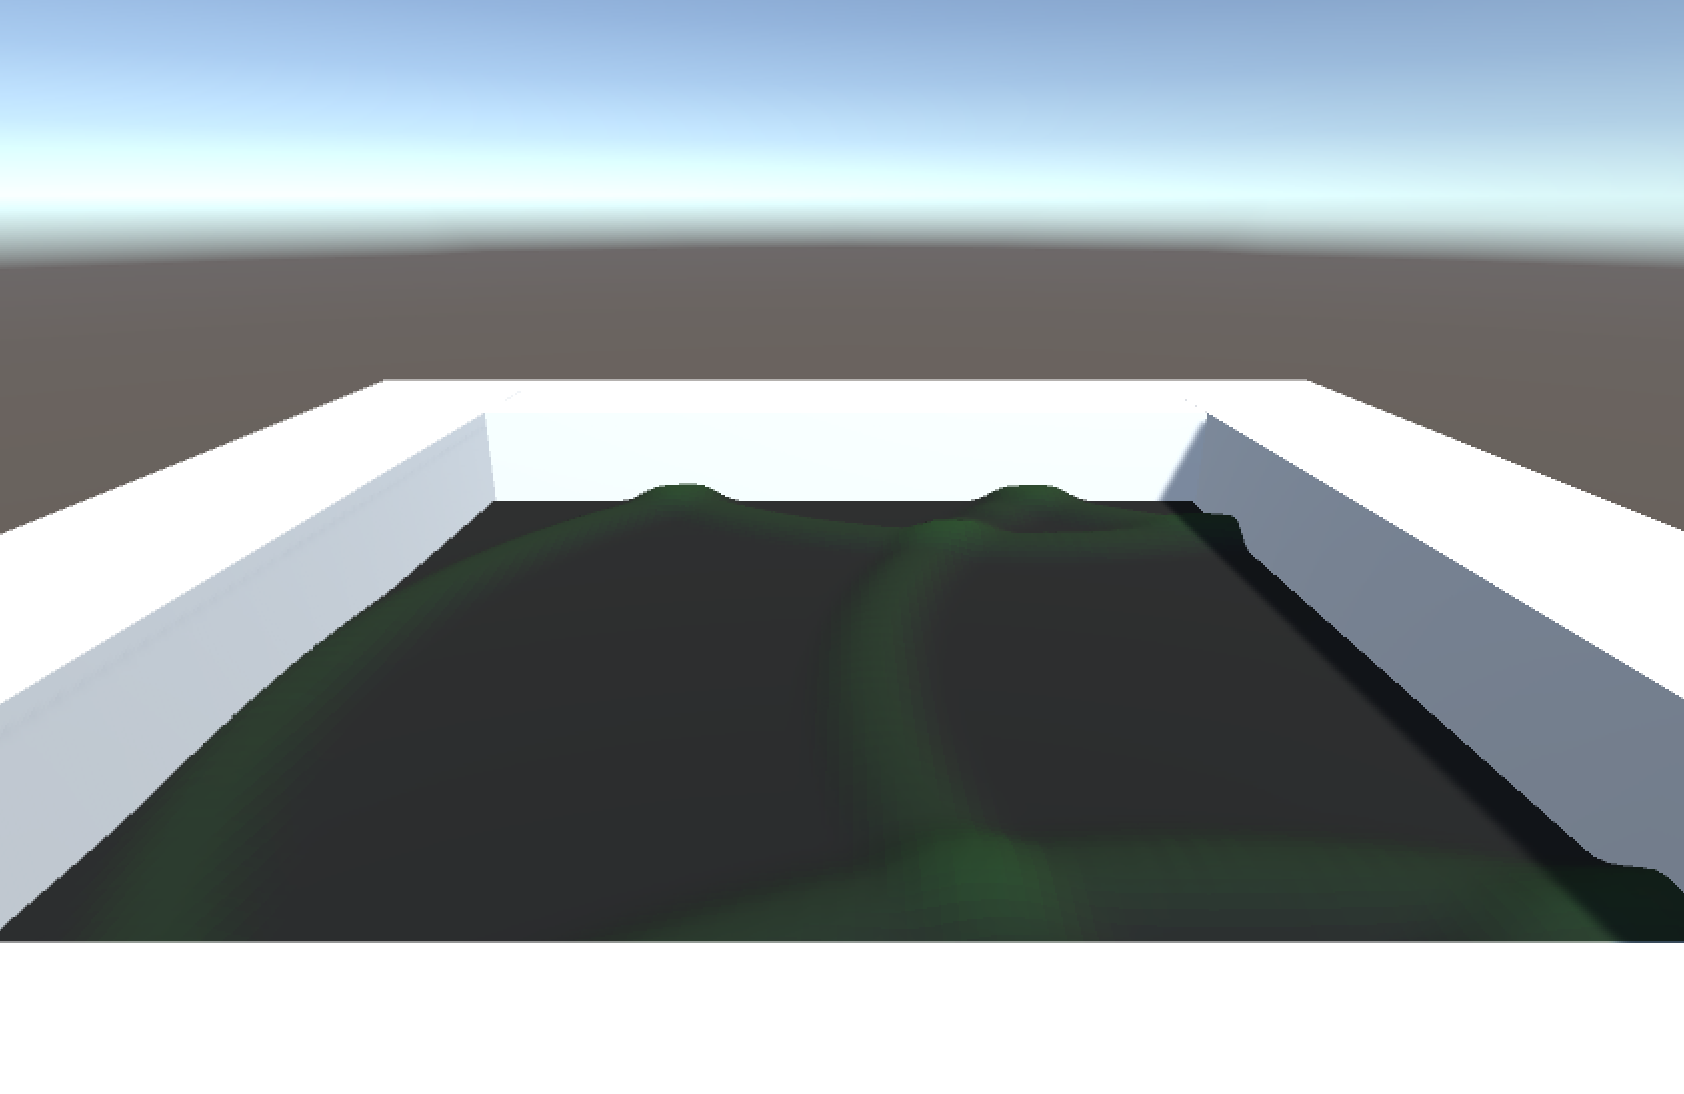
\includegraphics[width=0.8\linewidth]{wave_particle_reflections}
\caption{A screen shot of Wave Particles being reflected from my
implementation.}
\label{fig:wave_particle_reflections}
\end{figure}


\subsection{CPU Implementation}
\label{sec:implementation_splat_cpu}

Here I explain how I implemented the \texttt{ParticleContainer}
interface on the CPU. In particular, explaining how subdivisions were performed
in an efficient manner using a linked list. Finally, I justify the design
decisions I made.

I used a contiguous array of size $n$ to store Wave Particle data on the CPU.
This makes splatting them to a two-dimensional array in preparation for the
convolution stage both simple and of a fixed cost every frame. The array is
iterated over and for each Wave Particle, its position for the current frame is
calculated, and it is then drawn as a point-particle to the texture.

Furthermore, adding new particles to this data-structure is straightforward. I
treated the array as a cyclical buffer - with a pointer into the head.

In order to handle subdivisions, I used a single array of integers of size $m$,
the assumed maximum time before subdivision, to encode the event-table
described in Section \ref{sec:implementation_subdivision}. Each integer in this
array indexed a Wave Particle due to subdivide in the frame represented by the
table entry. If no Wave Particles were due to subdivide in a particular frame,
$-1$ was stored.

%TODO: Check with Alastair! (USE DIAGRAM)
As in a given frame, multiple Wave Particles could be due to subdivide, I used
a linked-list. In addition to the event-table, I made a \textit{link-table} of
integers of size $n$ that mirrored the Wave Particles array. Each entry in this
table was associated with the particle sharing its index. (eg. the tenth entry
in the link-table was associated with the tenth Wave Particle.) The entries in
the link-table represent indices to Wave Particles due to subdivide in the same
frame, forming a linked list.

In order to perform subdivisions for the current frame, $f$, the approach
described by the following C-like pseudocode is taken:

\begin{lstlisting}[language={C}]
void PerformSubdivisions(int f){
    // retrieve index of the first particle subdividing this frame
    int particle_index = event_table[f];
    // reset the event-table entry for the current frame
    event_table[f] = -1;
    // while particles are subdividing this frame
    while(particle_index != -1) {
        // retrieve particle subdividing this frame, subdivide it
        WaveParticle particle = particle_array[particle_index];
        PerformSubdivision(particle);

        // find the next subdividing particle
        int next_index = link_table[particle_index];
        // reset current entry in the link_table
        link_table[particle_index] = -1;
        // progress
        current_index = next_index;
    }
    return;
}
\end{lstlisting}

This setup is optimal for cache performance - originally the indices stored in
the link-table were stored with their associated Wave Particle in the array
\cite{Yuksel2007}. However, when splatting Wave Particles, this lead to the
cache being wasted, as the link data would be loaded with each Wave Particle.
So the decision was made to separate the two.

Wave Particle reflection can be plugged into the same system. I created a
separate event-table for particles due to reflect in a given frame, however the
link-table can be shared with the subdivision system. The reason for this is
that a Wave Particle cannot both subdivide and reflect in the same frame.

Here I focused on explaining the process of Wave Particle
subdivision on the CPU - how an event-table and link-table were used to index
the subset of Wave Particles that were due to subdivide each frame. I then
explained how this setup improved cache performance over the implementation
used in the original paper.

\subsection{GPU Implementation}

I describe how I implemented the \texttt{ParticleContainer} interface on
the GPU. In particular I explain how I used GPU compute shaders in a novel
manner, both to efficiently splat particles to a texture encoding the
displacement map and to perform subdivisions.

One of the main goals of storing and operating with Wave Particles on the GPU
was to make this process as quick and efficient as possible. The way I achieved
this was to minimise the amount of data that was transferred between the CPU
and the GPU.

Therefore, the CPU does not store a canonical source of Wave Particles data
that is copied to the GPU each frame. In fact, the CPU does not store any Wave
Particle information at all apart from a data-structure that is used for
handling subdivisions and queued Wave Particle additions. Previously, all Wave
Particles were stored in an array on the CPU and copied to the GPU every frame
for the purpose of being splatted to a texture \cite{Yuksel2007}.

I used an implementation of the \texttt{ParticleContainer} interface,
\texttt{GPUParticleContainer}, to handle all CPU-side code, while HLSL compute
shaders handled all GPU-side code. The Wave Particles themselves were stored in
a \texttt{ComputeBuffer} configured at initialise-time to be of the desired
size.

\subsubsection{Adding Particles}

One challenge was ensuring that adding particles to the GPU-side
\texttt{ComputeBuffer} was done in an efficient manner. Unity only provides
interfaces for copying a CPU-side array whole-sale into a
\texttt{ComputeBuffer}, which as mentioned before would be inefficient.

The efficient workaround to this was to have a CPU-side array that acts as a
buffer for particle additions. This buffer is flushed to a small
\texttt{ComputeBuffer} every frame, or if it fills up. A compute shader then
reads the small \texttt{ComputeBuffer} and adds all Wave Particles within it to
the main data-structure.

This is efficient as it ensures that rather than Wave Particles being copied
piecemeal to the GPU, the process is batched. Furthermore, the GPU can load all
of the batched data in parallel.

\subsubsection{Subdivisions}

% POSSIBLE: Delete Paragraph Below
This section will cover how subdivision was implemented in an efficient manner
- using the the strengths of the CPU in order to take advantage of assumptions
around the Wave Particle system. In addition to minimising the data transferred
from the CPU to the GPU in order to conserve that bottleneck.

I derived the GPU implementation of subdivision from the CPU one. Whilst the
GPU performed the subdivisions in parallel, the CPU still handled some of the
work - in particular walking through the link-table in an iterative manner.

An event-table and link-table were stored as arrays on the CPU, which held the
information of which Wave Particles were due to subdivide in any particular
frame, as described in Section \ref{sec:implementation_splat_cpu}. I programmed
the CPU to walk-through the indices of all the Wave Particles due to subdivide
in the current frame, storing them all in an array. I passed the array to the
GPU, which I had programmed to subdivide these particles in parallel. The GPU
also calculated which frames the new Wave Particles were due to subdivide in.
This data was copied back to the CPU so that it could be loaded into the
event-table and link-table.

% POSSIBLE: create figure.

\subsubsection{Splatting Particles}
% POSSIBLE- Move to Challenges: look at https://blogs.msdn.microsoft.com/ivanne/2012/01/04/multiple-ways-to-render-point-sprites-in-dx11/

Here I cover how Wave Particles are splatted to a texture using compute
shaders for the next stage of the pipeline, the issues the GPU implementation
faced, and the different anti-aliasing methods available in addition to their
benefits and drawbacks.

As shown in my evaluation - the GPU outperforms the CPU in its ability to draw
many Wave Particles in parallel to a texture as point particles. However, this
wasn't implemented without issues, as the parallelism led to some unavoidable
race conditions. Furthermore, efficient approaches to anti-aliasing needed to
be found.

Wave Particle splatting was implemented using a compute shader. This differed
from the implementation in the paper which used vertex and pixel shaders
\cite{Yuksel2007}. The compute shader was extremely simple; each thread being
responsible for splatting an individual particle to the displacement map
texture. The shader code calculated the position of the particle on the
two-dimensional plane.

%TODO: rewrite section, (Yuksel at al.) instead of "implementation in the paper""
% Yuksel et al achieved the desired implementation using a pixel shader... (CITE PAPER)
%TODO: look at non-workign reference

%TODO: have figure for artifacting?

There was a race condition when multiple GPU threads wanted to splat a Wave
Particle to the same pixel. The implementation in the paper did not suffer from
this, as it used a pixel shader to render point-sprites, which Unity did not
support \cite{NoPointSpritesUnityOne} \cite{NoPointSpritesUnityTwo}.
Additionally, the traditional solutions to this problem would have taken too
long to implement \cite{NoPointSpritesWorkaround}. I splatted the particles to
a higher resolution texture as a workaround - which reduced the chance of a
collision. I then wrote a custom shader to downsample this texture to the
desired resolution - with the added benefit of anti-aliasing. Figure
\ref{fig:downscale_example} shows an example of this.

% POSSIBLE: make this a diagram in inkscape
\begin{figure}[h]
\centering
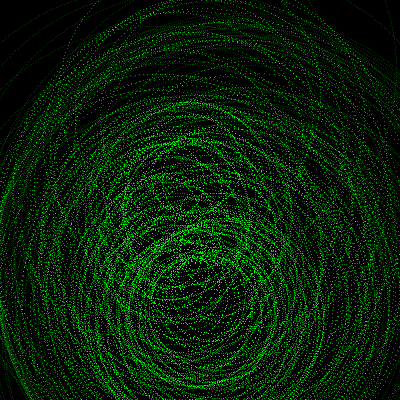
\includegraphics[width=0.6\linewidth]{splat_particles_large}
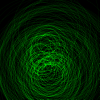
\includegraphics[width=0.3\linewidth]{splat_particles_downscale}
\caption{An example from my implementation of a 200 by 200 pixels texture being
downsampled to one that is 100 by 100 pixels.}
\label{fig:downscale_example}
\end{figure}
\section{Generating the Displacement Map through Convolution}

%TODO: rewrite section to not use class names?
Here I cover how the displacement map was generated. This
covers the techniques available on both the GPU and CPU.

This stage in the pipeline is represented by the \texttt{HeightFieldGenerator}
interface, with the important method being \texttt{GenerateHeightField()},
which takes an integer indicating the current frame and an
\texttt{ExtendedHeightField} instance encoding the results of the previous
stage. As \texttt{ExtendedHeightField} is a reference type; it is this argument
that also encodes the final output of this stage in the pipeline - that being
the final height-field as generated from the splatted Wave Particles.

As mentioned in Section
\ref{sec:implementation_overview_obtain_displacement_map}, the final
height-field can be obtained from the splatted Wave Particles using convolution.
However, the naive approach described in Section
\ref{sec:implementation_overview_obtain_displacement_map} of obtaining the
final displacement map was also implemented on the CPU as a reference.

\subsection{CPU Implementation}
\label{sec:implementation_convolution_cpu}

This section will cover how the final displacement map is generated on the CPU,
two methods of generating the displacement map were implemented:
Two-dimensional convolution and a brute-force naive approach.

The brute-force implementation simply iterates through every Wave Particle and
adds the appropriate displacement to each entry in the
\texttt{ExtendedHeightField} within the bounds of its radius as described by
Equation \ref{eq:particle_distortion}. I ensured the brute-force method
disabled Wave Particle splatting (as it is unnecessary), and this was the first
part of the Wave Particles system that I implemented.

I implemented the two-dimensional convolution method by pre-calculating a Wave
Particle kernel and storing it in a two-dimensional array of Vectors. The
implementation then convolves this kernel with the two-dimensional array stored
in the \texttt{ExtendedHeightField} input, and then returns the result.

\subsection{GPU Implementation}
\label{sec:implementation_convolution_gpu}

This was the first part of the Wave Particles system that I decided to
implement on the GPU. The reason for this being that GPUs are well suited to
graphical operations, and this could be easily done in a pixel shader as
opposed to a compute shader.

The convolution kernel is pre-calculated on the CPU into an array using the
method described in Section \ref{sec:implementation_convolution_cpu}, this
array in then copied to a texture on the GPU, where it is permanently stored.

When called, the GPU implementation renders a quad textured with the input
\texttt{ExtendedHeightField} of splatted Wave Particles. This is then convolved
in the pixel shader and output to a texture (Appendix
\ref{app:convolution_shader}). Figure \ref{fig:convolution_2D_example} shows
the result of this on the GPU as obtained from my implementation.

As this was the first part of the project I wrote, encountered some issues
as described in Section \ref{sec:evaluation_challenges}.

\section{Fluid-Object Interactions}

Here I describe how I generated Wave Particles by calculating the
volume of water displaced in a given frame, and how buoyancy was calculated
using submersion. 

The technique I used for fluid-object interaction was to render objects
orthogonally from a top-down perspective. I programmed the pixel shader to use
different color channels in the output to encode how submerged front and
back-facing parts the object were. I then used this information to calculate
the total submersion of a given object - which was used to calculate the
buoyancy force.

%TODO(Rafal): Diagram showing what is going on

The pixel shader also had access to the velocity of an object for a given frame,
this was used to calculate the amount of water displaced in a given frame, with
Wave Particles of an equivalent volume being generated on the surface.

This implementation could still use a lot of work and be extended, as it
currently based on some extremely limited heuristics. However, it does lead to
convincing results.
%TODO: Reference Figure

\section{Rendering}

This section will explain how I displaced vertices in a plane of triangles in
order to create a mesh of waves and how I used the Unity renderer to display
the mesh with convincing reflections.

In order to render the waves in three-dimensions, I placed a plane object in a
Unity scene. I then wrote a script, that when attached to the object, generates
a mesh of triangles with a resolution matching that of the image that is used
to encode the displacement map. I then displaced each vertex by the value
of the vector encoded in the corresponding pixel of the image. This can be seen
in Figure \ref{fig:vertex_example}.

\begin{figure}[h]
\centering
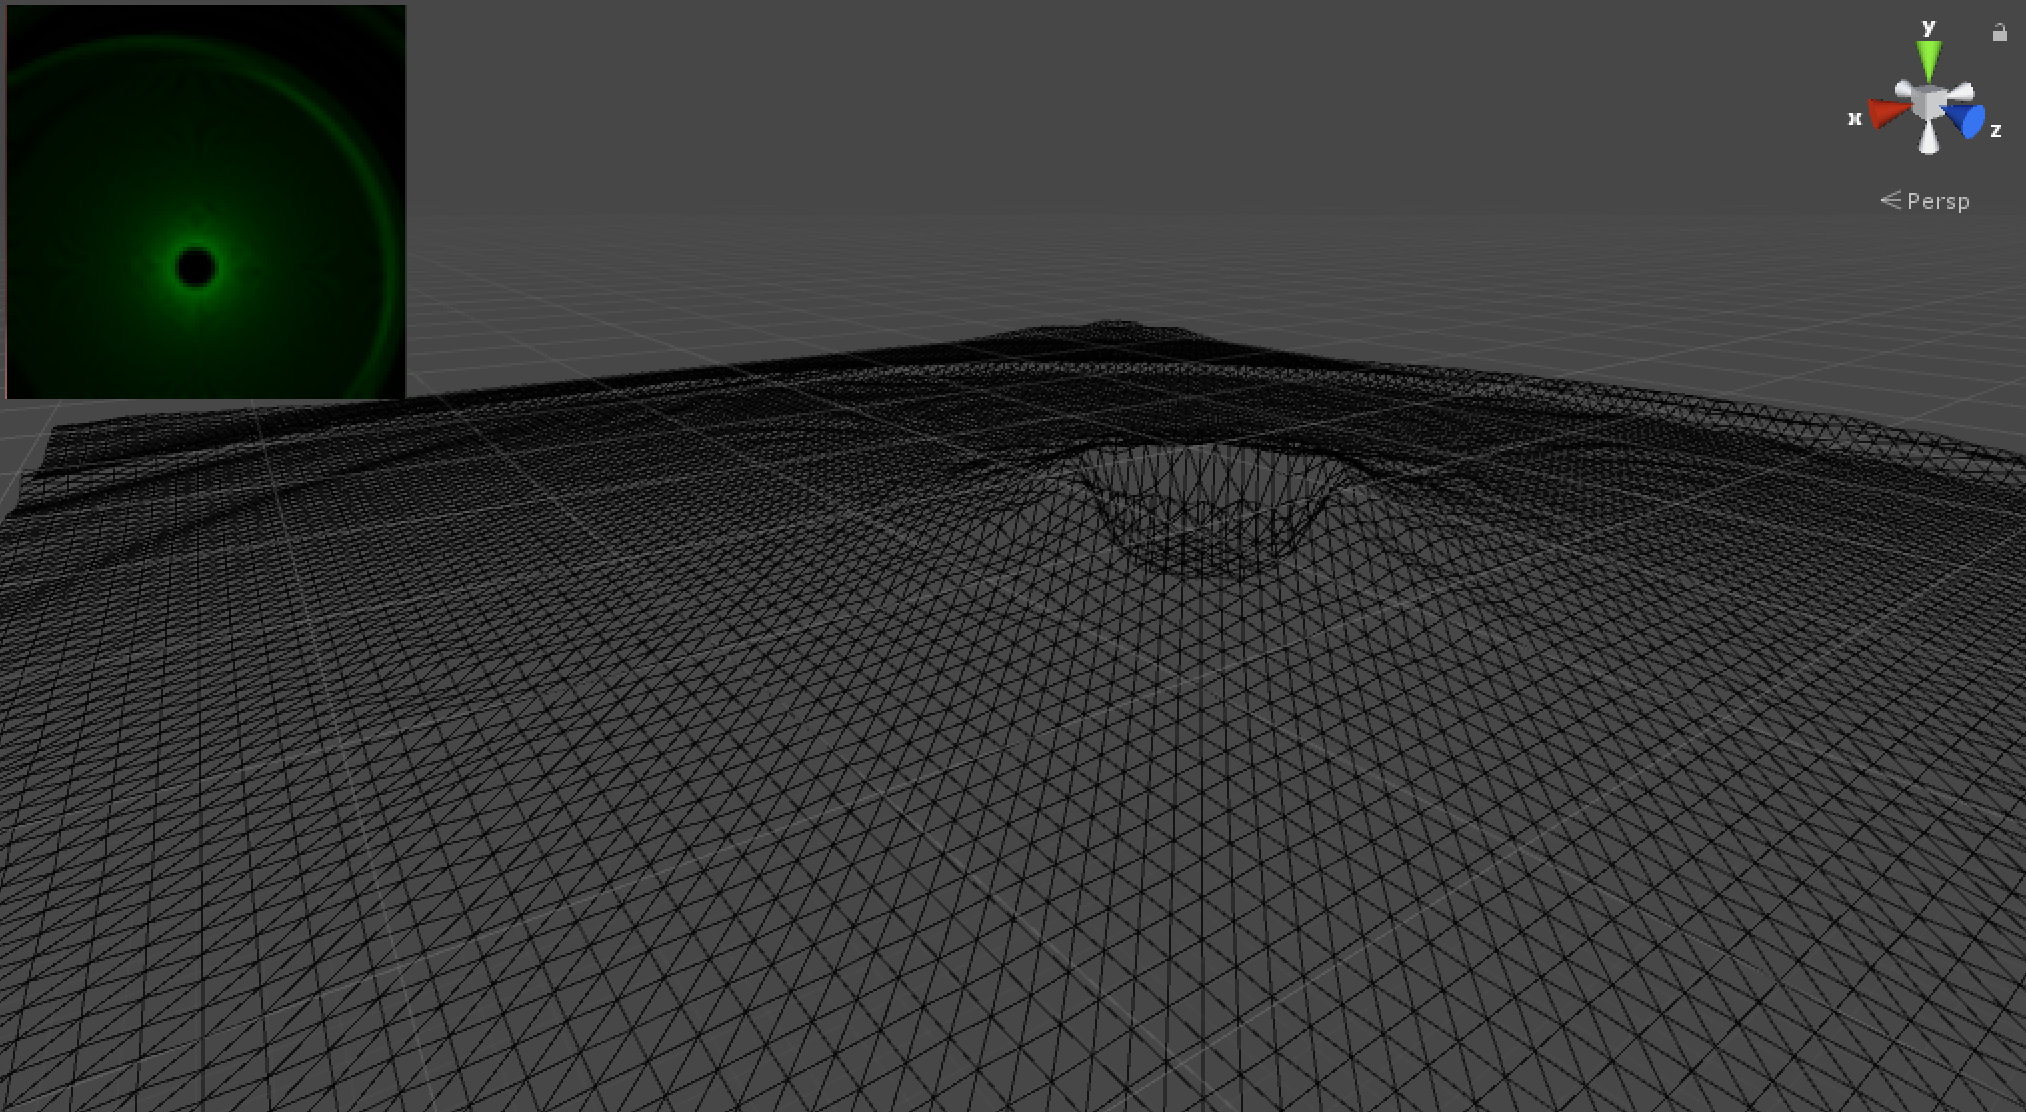
\includegraphics[width=0.8\linewidth]{vertex_example}
\caption{An image obtained from my implementation showing the two-dimensional
texture encoding the displacement map, alongside the generated mesh.}
\label{fig:vertex_example}
\end{figure}

I created both a CPU and GPU implementation of the vertex displacement
algorithm. Which implementation is used can be changed at runtime.

\subsection{Material Appearance}

Although not affecting the physical behaviour of the system, convincing visual
effects are an important part of fluid animation to show the type of fluid that
is being represented.

Refractive media such as water reflect a different proportion of light
depending on the angle at which light hits the surface, with reflection being
more likely at grazing angles. The equations which describe this, known as the
Fresnel equations, are typically approximated in real-time rendering using
Schlick's approximation (Equation \ref{eq:schlick}) \cite{Schlick94}.

\begin{equation} \label{eq:schlick}
\begin{split}
R(\theta) & = R_0 + (1 - R_0)(1 - \cos(\theta))^5 \\
R_0 & = (\frac{n_1 - n_2}{n_1 + n_2})^2
\end{split}
\end{equation}

$n_1$ and $n_2$ are the refractive indices of two media, while $\theta$ is the
difference between the direction of incident light and the normal of the
interface between the two media. The results of applying Equation
\ref{eq:schlick} to the project can be seen in Figure
\ref{fig:wave_particles_fresnel}.

\begin{figure}[h]
\centering
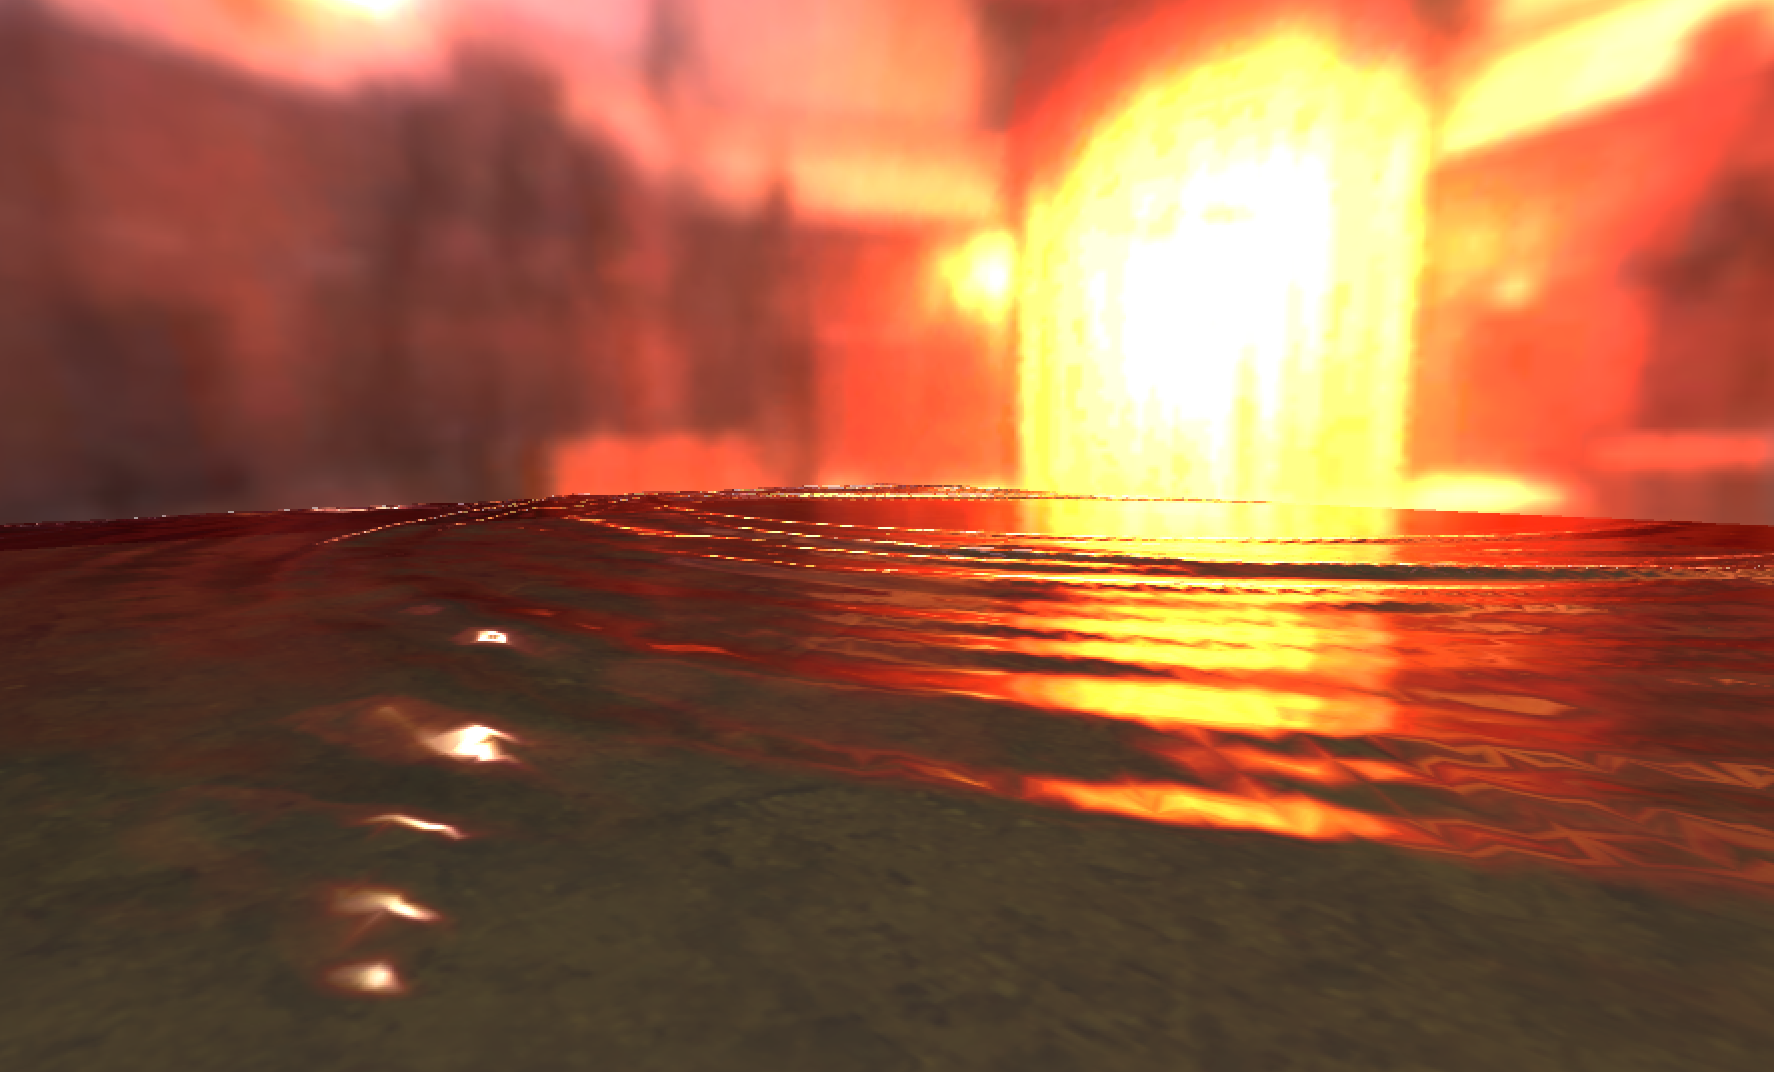
\includegraphics[width=0.8\linewidth]{wave_particles_fresnel}
\caption{An example from this project of Schlick's Approximation being used to
apply the Fresnel equations to the water. Light from the environment is
reflected at grazing angles while the waterbed can be seen head-on.}
\label{fig:wave_particles_fresnel}
\end{figure}

\section{Profiling \& Optimisation}

% MENTION Profiling
% MENTION how ExtendedHeightField was optimised
% MENTION how IEnumerator Garbage collection caused failures.
% https://msdn.microsoft.com/en-us/library/aa288257(v=vs.71).aspx
% http://stackoverflow.com/questions/18718399/every-iteration-of-every-foreach-loop-generated-24-bytes-of-garbage-memory
% http://stackoverflow.com/questions/5486654/allowing-iteration-without-generating-any-garbage

% https://github.com/steve3003/unity-profiler-data-exporter

% Unity Boxes STRUCTS in foreach loops! :(
%   http://www.gamasutra.com/blogs/WendelinReich/20131109/203841/C_Memory_Management_for_Unity_Developers_part_1_of_3.php
% )

% Here I explain how I optimised parts of the project, so as to
% improve the perfomance of my implementation. I first cover how Unity's
% profiler was used to determine critical paths in the code, then show general
% problems Unity and GPU programs can have.

% Finally, a couple of optimisation
% examples will be given, showing what was changed, why, how, the trade-offs that
% were made, and what the end results were.

% \subsection{Profiler}

Here I describe how the Unity profiler works and how I used it
to improve the perfomance of my implementation. I also cover the
limitations of the profiler before explaining how they were overcome.

Profiling is incredibly important in real-time graphics rendering, as it allows
critical paths and targets for optimisation to be found in a systematic manner.
Unity provides a \texttt{Profiler} class in the \texttt{UnityEngine.Profiling}
namespace with \texttt{BeginSample()} and \texttt{EndSample()} static methods
\cite{UnityProfiler}. The start of a sample can be named with a string, and it
is up to the programmer to ensure every sample is correctly enclosed.

When running the engine, the profiler will count how often each sample is
called, its total running time, the running time of each call to to it, the
amount of heap allocations and more. Importantly, the percentage of time of a
frame that was spent on a sample is recorded as well. The downside of adding
samples is that it slows down the program and clutters the code, something
which is ideally avoided.

As I wanted to keep track of areas of interest when profiling for when it came
time to evaluate the project; I created a branch in version control which was
kept up-to-date with the master branch - the only difference being that it
contained profiling statements around interesting parts of the code.

I found critical paths in the code by profiling the top-level update loop,
and identifying which calls took the most time each frame. I then iteratively
drilled down in order to find the program segments that took the most time or
allocated the most memory.

% OLD: Complete section

% \subsection{Common Unity Issues}

% % OLD: How they were solved
% As most code written in Unity is C\# - a garbage collected language, there are
% common pitfalls which can cause many Unity programs to suffer from performance
% issues. In fact, this has lead to Unity games having a reputation for
% inconsistent performance - expressed by frequent stuttering and hitching
% \cite{FirewatchDF} \cite{WhyUnityNeogaf}. However, these issues are by no means
% unavoidable, with a variety of techniques for avoiding them available when they
% arise.

% \subsubsection{Garbage Collection}

% The most common cause of performance issues in Unity programs is Garbage
% Collection, so minimising it is extremely important \cite{UnityPerformanceTipsGamaSutra}
% \cite{MemoryManagementUnityGamaSutra}.

% \subsubsection{Multithreading}

% Multithreading support in Unity is extremely limited \cite{UnityBadThreading}
% \cite{FirewatchDF}.

% \subsection{Examples of Optimisation}

% Here I go through process I used to identify and optimise parts
% of the Wave Particles system, the performance gains these led to, the tradeoffs
% that had to be made and the challenges that were faced.

% \subsubsection{Convolution CPU Garbage}

% Here...

% \subsubsection{Foreach trouble}

% Unity provides an interface for making classes iterable, so that you can loop
% over elements of them. Doing so is very straight forward. You simply implement
% the \texttt{System.Collections.IEnumerable } class. Another options is to use
% co-routines. However, both of these things so cause issues, as Unity will
% allocate some memory to the heap each time you iterate over on object that uses
% these \cite{UnityForeachGarbageStack} \cite{CShaprForeachWithCollections}.

% A solution to this is to implement the interface manually using a struct, as
% structs in C\# are allocated on the stack instead of the heap
% \cite{CSharpIterationStructs}. Which is what I did.

% Unfortunately, after doing this, even though the amount of garbage generated
% had descreased, on profiling there was still garbage being generated.

% After investigation, this was a result of a bug in the C\# compiler that Unity
% uses \cite{MemoryManagementUnityGamaSutra}. 

\section{Summary}

In this chapter I gave an overview of the theory guiding the implementation -
specifically some of the approximations and assumptions that could be made in
order to pre-compute subdivision events and perform convolution to obtain the
final height-field. I then went into some details about programming for the
GPU, and how I approached doing that. Following that, I described the data
structures I used in my implementation before explaining the algorithms and
systems I used - including how I used compute shaders in a novel manner to
limit the amount of data transferred between the GPU and CPU. I finally
explained how I used Unity's profiler in order to optimise the code.

\chapter{Evaluation}

In this chapter, I analyse the memory usage and perfomance of the Wave
Particles system across the GPU and CPU. I then describe some of the challenges
I faced, mainly describing in depth the friction that shader programming
caused. Finally, I analyse the success criteria I set in the project proposal
and demonstrate how I met them and completed two extensions.

All performance measurements were performed on a Microsoft Surface Book
containing a 2.60GHz 4-core Intel i7-6600U CPU and 16GBs of Memory. The GPU
has no commercial equivalent, but is comparable to an 940m entry-level laptop
GPU by Nvidia in performance \cite{CNETSurfaceBookGPU}
\cite{HEXUSSurfaceBookGPU}.

\section{Memory}
\label{sec:evaluation_memory}

Here I explain how I overcame some of the issues caused by the
C\# garbage collector. I then analyse the memory usage of both the Wave
Particles container and the displacement map.

% OLD
% Memory usage is incredibly important in real-time graphics applications as
% different components in a system need to compete for limited resources.
% Furthermore, many strategies can exist for solving certain problems with a
% tradeoff of performance against memory usage.

\subsection{C\# Garbage Collection}

As most code written in Unity is C\# - a garbage collected language, memory
usage can cause many Unity programs to suffer from performance issues. In fact,
this has lead to Unity games having a reputation for inconsistent performance -
expressed by frequent stuttering and hitching \cite{FirewatchDF}
\cite{WhyUnityNeogaf}. However, I overcame these issues by using object pooling
\cite{UnityObjectPooling}, which was possible as memory usage in the Wave
Particles system is constant: All the memory that is required for any
particular set-up can be pre-allocated at load-time.

\subsection{Wave Particle Container}

The Wave Particle container has two components of independent sizes, a cyclic
array of Wave Particles (mirrored by the link table) and an event-table. The
data-structures of the CPU and the GPU implementations have identical memory
requirements - simply differing in the location where they are stored. I will
demonstrate why the Wave Particles system is incredibly lightweight and
therefore suitable for memory-limited real-time systems.

A Wave Particle is $28$ bytes, and each is mirrored by a link table entry of
$4$ bytes. Therefore, a system of $n$ particles requires one array that is
$28n$ bytes, with an additional array that is $4n$ bytes large. For example, a
system with 500,000 Wave Particles will require $13.35MiB$ for the Wave
Particles array and $2.91MiB$ for the link table.

As discussed in Section \ref{sec:implementation_subdivision}, the size of the
event-table should be larger than the separation time between most events.
Equation \ref{eq:subdivision_calc} can be modified and used to determine an
appropriate size of the table: Given a system where Wave Particles have a given
radius $r_{wp}$ and speed $u_{wp}$, and the frame time is $t_f$, the size $S$
of an event-table that can accurately be used to store subdivision events down
to a given dispersion angle $\theta_{wp}$ is described by Equation
\ref{eq:subdivision_event_size_calc}.

\begin{equation}
\label{eq:subdivision_event_size_calc}
S = \frac{r_{wp}}{2 u_{wp} \theta_{wp} t_f}
\end{equation}

For example, given $r_{wp}=0.2m$, $u_{wp}=1ms^{-1}$, and $t_f=0.017s$, the time
until a subdivision event caused by a dispersion angle of 0.0006 radians
requires an event-table with less than 10,000 entries. This is the approach I
took, only requiring $40KiB$.

\subsection{Splatting and Convolution - The Displacement Map}

The amount of memory required for splatting and convolution depends on the
implementation used, the resolution of the displacement map, and the resolution
of the convolution kernel (if any).

The implementation used affects the number and sizes of copies of the
displacement map that are required - from the naive CPU implementation
requiring one copy, to the most effective GPU implementation requiring three
copies in addition to the convolution kernel.

As the displacement map is represented by an $n$ by $m$ image, where each pixel
is 16 bytes, the amount of space it occupies is $16nm$ bytes. Therefore in a
system with a resolution of 100 by 100, the amount of space required for each
map is 16KiB - which is negligible compared to the size of the Wave Particles
container.

However, the resolution of the displacement map also affects the size of the
mesh used to render the water - of which two copies are kept as both inputs and
outputs of the vertex shader. As the meshes are handled by Unity, I used
RenderDoc in order to calculate the effect resolution had on the memory;
looking at the effect different resolutions had on the size of the mesh. The
size of the mesh was closely correlated to the number of vertices it had, with
297 to 306 bytes being required per vertex. The raw data can be seen in Figure
\ref{fig:table_mesh_sizes}. Therefore, in the typical case of a 100 by 100
displacement map, 2.9MiB is required for the mesh.

\begin{figure}[h]
\begin{center}
\begin{tabular}{|c | c c |} 
\hline
 Displacement Map Resolution & Size (bytes) & Bytes per Vertex\\ [0.5ex] 
\hline\hline
25x100 & 741,312 & 297 \\ 
\hline
50x50 & 749,112  & 300 \\
\hline
50x100 & 1,513,512 & 303 \\
\hline
100x100 & 3,057,912 & 306 \\ [1ex] 
\hline
\end{tabular}
\end{center}
\caption{Table showing how the resolution of the displacement map affects the
size the water mesh occupied in memory.}
\label{fig:table_mesh_sizes}
\end{figure}

\subsection{Conclusion}

By modern standards, the Wave Particles system has a very light memory
footprint. A system with 500,000 Wave Particle and a 100 by 100 displacement
map has a 50MiB footprint - which is $0.6\%$ of the $8GiB$ of memory a typical
gaming system such as the PlayStation 4 has \cite{DFPS4}. This means that the
Wave Particles system is suitable for real-time applications from a memory
usage perspective.

\section{Performance}

Here I evaluate the perfomance of both splatting Wave
Particles and Convolution - the principle components of the Wave Particles
system. This will be done by profiling the execution of the functions of
interest for 300 frames under various conditions - before I analyse the results
to compare and contrast how both the CPU and the GPU perform.

\subsection{Splatting Wave Particles}

Here the CPU and GPU implementation of Wave Particle Splatting will
be analysed and compared. The systems will be observed operating for 300
frames. How the GPU vastly outperforms the CPU will be shown, in addition to
how the performance gap widens with larger numbers of Wave Particles.

As explained in Section \ref{sec:storing_subdividing_splatting}, Wave Particles
are splatted as point-particles to an image, and this is defined in the
\texttt{SetPointMap()} method of an interface named \texttt{ParticleContainer}.
There are two implementations of this interface, one on the GPU and one on the
CPU.

In order to compare how the performance of these implementations scaled, I
captured 300 frames of a system with a systematically increasing number of Wave
Particles using the Unity Profiler and exported that data using the
\textit{Unity Profiler Data Exporter} \cite{UnityProfilerDataExporter}. The
conditions under which the system was profiled are given in Appendix
\ref{app:performance_graphs_splatting}.

Figure \ref{fig:graph_set_point_map_10000} shows how the system performs over
time with 10,000 Wave Particles. The GPU, taking $1.64ms$ per frame, has a
four-fold performance improvement over the CPU's $8.31ms$. Considering a 30FPS
a performance budget of $33ms$, the GPU implementation would take $4.92\%$ of
the total.

\begin{figure}[h]
\centering
%% Creator: Matplotlib, PGF backend
%%
%% To include the figure in your LaTeX document, write
%%   \input{<filename>.pgf}
%%
%% Make sure the required packages are loaded in your preamble
%%   \usepackage{pgf}
%%
%% Figures using additional raster images can only be included by \input if
%% they are in the same directory as the main LaTeX file. For loading figures
%% from other directories you can use the `import` package
%%   \usepackage{import}
%% and then include the figures with
%%   \import{<path to file>}{<filename>.pgf}
%%
%% Matplotlib used the following preamble
%%   \usepackage{fontspec}
%%
\begingroup%
\makeatletter%
\begin{pgfpicture}%
\pgfpathrectangle{\pgfpointorigin}{\pgfqpoint{6.400000in}{4.800000in}}%
\pgfusepath{use as bounding box, clip}%
\begin{pgfscope}%
\pgfsetbuttcap%
\pgfsetmiterjoin%
\definecolor{currentfill}{rgb}{1.000000,1.000000,1.000000}%
\pgfsetfillcolor{currentfill}%
\pgfsetlinewidth{0.000000pt}%
\definecolor{currentstroke}{rgb}{1.000000,1.000000,1.000000}%
\pgfsetstrokecolor{currentstroke}%
\pgfsetdash{}{0pt}%
\pgfpathmoveto{\pgfqpoint{0.000000in}{0.000000in}}%
\pgfpathlineto{\pgfqpoint{6.400000in}{0.000000in}}%
\pgfpathlineto{\pgfqpoint{6.400000in}{4.800000in}}%
\pgfpathlineto{\pgfqpoint{0.000000in}{4.800000in}}%
\pgfpathclose%
\pgfusepath{fill}%
\end{pgfscope}%
\begin{pgfscope}%
\pgfsetbuttcap%
\pgfsetmiterjoin%
\definecolor{currentfill}{rgb}{0.898039,0.898039,0.898039}%
\pgfsetfillcolor{currentfill}%
\pgfsetlinewidth{0.000000pt}%
\definecolor{currentstroke}{rgb}{0.000000,0.000000,0.000000}%
\pgfsetstrokecolor{currentstroke}%
\pgfsetstrokeopacity{0.000000}%
\pgfsetdash{}{0pt}%
\pgfpathmoveto{\pgfqpoint{0.800000in}{0.528000in}}%
\pgfpathlineto{\pgfqpoint{5.760000in}{0.528000in}}%
\pgfpathlineto{\pgfqpoint{5.760000in}{4.224000in}}%
\pgfpathlineto{\pgfqpoint{0.800000in}{4.224000in}}%
\pgfpathclose%
\pgfusepath{fill}%
\end{pgfscope}%
\begin{pgfscope}%
\pgfpathrectangle{\pgfqpoint{0.800000in}{0.528000in}}{\pgfqpoint{4.960000in}{3.696000in}} %
\pgfusepath{clip}%
\pgfsetrectcap%
\pgfsetroundjoin%
\pgfsetlinewidth{0.803000pt}%
\definecolor{currentstroke}{rgb}{1.000000,1.000000,1.000000}%
\pgfsetstrokecolor{currentstroke}%
\pgfsetdash{}{0pt}%
\pgfpathmoveto{\pgfqpoint{0.800000in}{0.528000in}}%
\pgfpathlineto{\pgfqpoint{0.800000in}{4.224000in}}%
\pgfusepath{stroke}%
\end{pgfscope}%
\begin{pgfscope}%
\pgfsetbuttcap%
\pgfsetroundjoin%
\definecolor{currentfill}{rgb}{0.333333,0.333333,0.333333}%
\pgfsetfillcolor{currentfill}%
\pgfsetlinewidth{0.803000pt}%
\definecolor{currentstroke}{rgb}{0.333333,0.333333,0.333333}%
\pgfsetstrokecolor{currentstroke}%
\pgfsetdash{}{0pt}%
\pgfsys@defobject{currentmarker}{\pgfqpoint{0.000000in}{-0.048611in}}{\pgfqpoint{0.000000in}{0.000000in}}{%
\pgfpathmoveto{\pgfqpoint{0.000000in}{0.000000in}}%
\pgfpathlineto{\pgfqpoint{0.000000in}{-0.048611in}}%
\pgfusepath{stroke,fill}%
}%
\begin{pgfscope}%
\pgfsys@transformshift{0.800000in}{0.528000in}%
\pgfsys@useobject{currentmarker}{}%
\end{pgfscope}%
\end{pgfscope}%
\begin{pgfscope}%
\definecolor{textcolor}{rgb}{0.333333,0.333333,0.333333}%
\pgfsetstrokecolor{textcolor}%
\pgfsetfillcolor{textcolor}%
\pgftext[x=0.800000in,y=0.430778in,,top]{\color{textcolor}\rmfamily\fontsize{10.000000}{12.000000}\selectfont \(\displaystyle 0\)}%
\end{pgfscope}%
\begin{pgfscope}%
\pgfpathrectangle{\pgfqpoint{0.800000in}{0.528000in}}{\pgfqpoint{4.960000in}{3.696000in}} %
\pgfusepath{clip}%
\pgfsetrectcap%
\pgfsetroundjoin%
\pgfsetlinewidth{0.803000pt}%
\definecolor{currentstroke}{rgb}{1.000000,1.000000,1.000000}%
\pgfsetstrokecolor{currentstroke}%
\pgfsetdash{}{0pt}%
\pgfpathmoveto{\pgfqpoint{1.629431in}{0.528000in}}%
\pgfpathlineto{\pgfqpoint{1.629431in}{4.224000in}}%
\pgfusepath{stroke}%
\end{pgfscope}%
\begin{pgfscope}%
\pgfsetbuttcap%
\pgfsetroundjoin%
\definecolor{currentfill}{rgb}{0.333333,0.333333,0.333333}%
\pgfsetfillcolor{currentfill}%
\pgfsetlinewidth{0.803000pt}%
\definecolor{currentstroke}{rgb}{0.333333,0.333333,0.333333}%
\pgfsetstrokecolor{currentstroke}%
\pgfsetdash{}{0pt}%
\pgfsys@defobject{currentmarker}{\pgfqpoint{0.000000in}{-0.048611in}}{\pgfqpoint{0.000000in}{0.000000in}}{%
\pgfpathmoveto{\pgfqpoint{0.000000in}{0.000000in}}%
\pgfpathlineto{\pgfqpoint{0.000000in}{-0.048611in}}%
\pgfusepath{stroke,fill}%
}%
\begin{pgfscope}%
\pgfsys@transformshift{1.629431in}{0.528000in}%
\pgfsys@useobject{currentmarker}{}%
\end{pgfscope}%
\end{pgfscope}%
\begin{pgfscope}%
\definecolor{textcolor}{rgb}{0.333333,0.333333,0.333333}%
\pgfsetstrokecolor{textcolor}%
\pgfsetfillcolor{textcolor}%
\pgftext[x=1.629431in,y=0.430778in,,top]{\color{textcolor}\rmfamily\fontsize{10.000000}{12.000000}\selectfont \(\displaystyle 50\)}%
\end{pgfscope}%
\begin{pgfscope}%
\pgfpathrectangle{\pgfqpoint{0.800000in}{0.528000in}}{\pgfqpoint{4.960000in}{3.696000in}} %
\pgfusepath{clip}%
\pgfsetrectcap%
\pgfsetroundjoin%
\pgfsetlinewidth{0.803000pt}%
\definecolor{currentstroke}{rgb}{1.000000,1.000000,1.000000}%
\pgfsetstrokecolor{currentstroke}%
\pgfsetdash{}{0pt}%
\pgfpathmoveto{\pgfqpoint{2.458863in}{0.528000in}}%
\pgfpathlineto{\pgfqpoint{2.458863in}{4.224000in}}%
\pgfusepath{stroke}%
\end{pgfscope}%
\begin{pgfscope}%
\pgfsetbuttcap%
\pgfsetroundjoin%
\definecolor{currentfill}{rgb}{0.333333,0.333333,0.333333}%
\pgfsetfillcolor{currentfill}%
\pgfsetlinewidth{0.803000pt}%
\definecolor{currentstroke}{rgb}{0.333333,0.333333,0.333333}%
\pgfsetstrokecolor{currentstroke}%
\pgfsetdash{}{0pt}%
\pgfsys@defobject{currentmarker}{\pgfqpoint{0.000000in}{-0.048611in}}{\pgfqpoint{0.000000in}{0.000000in}}{%
\pgfpathmoveto{\pgfqpoint{0.000000in}{0.000000in}}%
\pgfpathlineto{\pgfqpoint{0.000000in}{-0.048611in}}%
\pgfusepath{stroke,fill}%
}%
\begin{pgfscope}%
\pgfsys@transformshift{2.458863in}{0.528000in}%
\pgfsys@useobject{currentmarker}{}%
\end{pgfscope}%
\end{pgfscope}%
\begin{pgfscope}%
\definecolor{textcolor}{rgb}{0.333333,0.333333,0.333333}%
\pgfsetstrokecolor{textcolor}%
\pgfsetfillcolor{textcolor}%
\pgftext[x=2.458863in,y=0.430778in,,top]{\color{textcolor}\rmfamily\fontsize{10.000000}{12.000000}\selectfont \(\displaystyle 100\)}%
\end{pgfscope}%
\begin{pgfscope}%
\pgfpathrectangle{\pgfqpoint{0.800000in}{0.528000in}}{\pgfqpoint{4.960000in}{3.696000in}} %
\pgfusepath{clip}%
\pgfsetrectcap%
\pgfsetroundjoin%
\pgfsetlinewidth{0.803000pt}%
\definecolor{currentstroke}{rgb}{1.000000,1.000000,1.000000}%
\pgfsetstrokecolor{currentstroke}%
\pgfsetdash{}{0pt}%
\pgfpathmoveto{\pgfqpoint{3.288294in}{0.528000in}}%
\pgfpathlineto{\pgfqpoint{3.288294in}{4.224000in}}%
\pgfusepath{stroke}%
\end{pgfscope}%
\begin{pgfscope}%
\pgfsetbuttcap%
\pgfsetroundjoin%
\definecolor{currentfill}{rgb}{0.333333,0.333333,0.333333}%
\pgfsetfillcolor{currentfill}%
\pgfsetlinewidth{0.803000pt}%
\definecolor{currentstroke}{rgb}{0.333333,0.333333,0.333333}%
\pgfsetstrokecolor{currentstroke}%
\pgfsetdash{}{0pt}%
\pgfsys@defobject{currentmarker}{\pgfqpoint{0.000000in}{-0.048611in}}{\pgfqpoint{0.000000in}{0.000000in}}{%
\pgfpathmoveto{\pgfqpoint{0.000000in}{0.000000in}}%
\pgfpathlineto{\pgfqpoint{0.000000in}{-0.048611in}}%
\pgfusepath{stroke,fill}%
}%
\begin{pgfscope}%
\pgfsys@transformshift{3.288294in}{0.528000in}%
\pgfsys@useobject{currentmarker}{}%
\end{pgfscope}%
\end{pgfscope}%
\begin{pgfscope}%
\definecolor{textcolor}{rgb}{0.333333,0.333333,0.333333}%
\pgfsetstrokecolor{textcolor}%
\pgfsetfillcolor{textcolor}%
\pgftext[x=3.288294in,y=0.430778in,,top]{\color{textcolor}\rmfamily\fontsize{10.000000}{12.000000}\selectfont \(\displaystyle 150\)}%
\end{pgfscope}%
\begin{pgfscope}%
\pgfpathrectangle{\pgfqpoint{0.800000in}{0.528000in}}{\pgfqpoint{4.960000in}{3.696000in}} %
\pgfusepath{clip}%
\pgfsetrectcap%
\pgfsetroundjoin%
\pgfsetlinewidth{0.803000pt}%
\definecolor{currentstroke}{rgb}{1.000000,1.000000,1.000000}%
\pgfsetstrokecolor{currentstroke}%
\pgfsetdash{}{0pt}%
\pgfpathmoveto{\pgfqpoint{4.117726in}{0.528000in}}%
\pgfpathlineto{\pgfqpoint{4.117726in}{4.224000in}}%
\pgfusepath{stroke}%
\end{pgfscope}%
\begin{pgfscope}%
\pgfsetbuttcap%
\pgfsetroundjoin%
\definecolor{currentfill}{rgb}{0.333333,0.333333,0.333333}%
\pgfsetfillcolor{currentfill}%
\pgfsetlinewidth{0.803000pt}%
\definecolor{currentstroke}{rgb}{0.333333,0.333333,0.333333}%
\pgfsetstrokecolor{currentstroke}%
\pgfsetdash{}{0pt}%
\pgfsys@defobject{currentmarker}{\pgfqpoint{0.000000in}{-0.048611in}}{\pgfqpoint{0.000000in}{0.000000in}}{%
\pgfpathmoveto{\pgfqpoint{0.000000in}{0.000000in}}%
\pgfpathlineto{\pgfqpoint{0.000000in}{-0.048611in}}%
\pgfusepath{stroke,fill}%
}%
\begin{pgfscope}%
\pgfsys@transformshift{4.117726in}{0.528000in}%
\pgfsys@useobject{currentmarker}{}%
\end{pgfscope}%
\end{pgfscope}%
\begin{pgfscope}%
\definecolor{textcolor}{rgb}{0.333333,0.333333,0.333333}%
\pgfsetstrokecolor{textcolor}%
\pgfsetfillcolor{textcolor}%
\pgftext[x=4.117726in,y=0.430778in,,top]{\color{textcolor}\rmfamily\fontsize{10.000000}{12.000000}\selectfont \(\displaystyle 200\)}%
\end{pgfscope}%
\begin{pgfscope}%
\pgfpathrectangle{\pgfqpoint{0.800000in}{0.528000in}}{\pgfqpoint{4.960000in}{3.696000in}} %
\pgfusepath{clip}%
\pgfsetrectcap%
\pgfsetroundjoin%
\pgfsetlinewidth{0.803000pt}%
\definecolor{currentstroke}{rgb}{1.000000,1.000000,1.000000}%
\pgfsetstrokecolor{currentstroke}%
\pgfsetdash{}{0pt}%
\pgfpathmoveto{\pgfqpoint{4.947157in}{0.528000in}}%
\pgfpathlineto{\pgfqpoint{4.947157in}{4.224000in}}%
\pgfusepath{stroke}%
\end{pgfscope}%
\begin{pgfscope}%
\pgfsetbuttcap%
\pgfsetroundjoin%
\definecolor{currentfill}{rgb}{0.333333,0.333333,0.333333}%
\pgfsetfillcolor{currentfill}%
\pgfsetlinewidth{0.803000pt}%
\definecolor{currentstroke}{rgb}{0.333333,0.333333,0.333333}%
\pgfsetstrokecolor{currentstroke}%
\pgfsetdash{}{0pt}%
\pgfsys@defobject{currentmarker}{\pgfqpoint{0.000000in}{-0.048611in}}{\pgfqpoint{0.000000in}{0.000000in}}{%
\pgfpathmoveto{\pgfqpoint{0.000000in}{0.000000in}}%
\pgfpathlineto{\pgfqpoint{0.000000in}{-0.048611in}}%
\pgfusepath{stroke,fill}%
}%
\begin{pgfscope}%
\pgfsys@transformshift{4.947157in}{0.528000in}%
\pgfsys@useobject{currentmarker}{}%
\end{pgfscope}%
\end{pgfscope}%
\begin{pgfscope}%
\definecolor{textcolor}{rgb}{0.333333,0.333333,0.333333}%
\pgfsetstrokecolor{textcolor}%
\pgfsetfillcolor{textcolor}%
\pgftext[x=4.947157in,y=0.430778in,,top]{\color{textcolor}\rmfamily\fontsize{10.000000}{12.000000}\selectfont \(\displaystyle 250\)}%
\end{pgfscope}%
\begin{pgfscope}%
\definecolor{textcolor}{rgb}{0.333333,0.333333,0.333333}%
\pgfsetstrokecolor{textcolor}%
\pgfsetfillcolor{textcolor}%
\pgftext[x=3.280000in,y=0.251889in,,top]{\color{textcolor}\rmfamily\fontsize{12.000000}{14.400000}\selectfont Frame Number}%
\end{pgfscope}%
\begin{pgfscope}%
\pgfpathrectangle{\pgfqpoint{0.800000in}{0.528000in}}{\pgfqpoint{4.960000in}{3.696000in}} %
\pgfusepath{clip}%
\pgfsetrectcap%
\pgfsetroundjoin%
\pgfsetlinewidth{0.803000pt}%
\definecolor{currentstroke}{rgb}{1.000000,1.000000,1.000000}%
\pgfsetstrokecolor{currentstroke}%
\pgfsetdash{}{0pt}%
\pgfpathmoveto{\pgfqpoint{0.800000in}{0.903123in}}%
\pgfpathlineto{\pgfqpoint{5.760000in}{0.903123in}}%
\pgfusepath{stroke}%
\end{pgfscope}%
\begin{pgfscope}%
\pgfsetbuttcap%
\pgfsetroundjoin%
\definecolor{currentfill}{rgb}{0.333333,0.333333,0.333333}%
\pgfsetfillcolor{currentfill}%
\pgfsetlinewidth{0.803000pt}%
\definecolor{currentstroke}{rgb}{0.333333,0.333333,0.333333}%
\pgfsetstrokecolor{currentstroke}%
\pgfsetdash{}{0pt}%
\pgfsys@defobject{currentmarker}{\pgfqpoint{-0.048611in}{0.000000in}}{\pgfqpoint{0.000000in}{0.000000in}}{%
\pgfpathmoveto{\pgfqpoint{0.000000in}{0.000000in}}%
\pgfpathlineto{\pgfqpoint{-0.048611in}{0.000000in}}%
\pgfusepath{stroke,fill}%
}%
\begin{pgfscope}%
\pgfsys@transformshift{0.800000in}{0.903123in}%
\pgfsys@useobject{currentmarker}{}%
\end{pgfscope}%
\end{pgfscope}%
\begin{pgfscope}%
\definecolor{textcolor}{rgb}{0.333333,0.333333,0.333333}%
\pgfsetstrokecolor{textcolor}%
\pgfsetfillcolor{textcolor}%
\pgftext[x=0.633333in,y=0.854929in,left,base]{\color{textcolor}\rmfamily\fontsize{10.000000}{12.000000}\selectfont \(\displaystyle 2\)}%
\end{pgfscope}%
\begin{pgfscope}%
\pgfpathrectangle{\pgfqpoint{0.800000in}{0.528000in}}{\pgfqpoint{4.960000in}{3.696000in}} %
\pgfusepath{clip}%
\pgfsetrectcap%
\pgfsetroundjoin%
\pgfsetlinewidth{0.803000pt}%
\definecolor{currentstroke}{rgb}{1.000000,1.000000,1.000000}%
\pgfsetstrokecolor{currentstroke}%
\pgfsetdash{}{0pt}%
\pgfpathmoveto{\pgfqpoint{0.800000in}{1.478466in}}%
\pgfpathlineto{\pgfqpoint{5.760000in}{1.478466in}}%
\pgfusepath{stroke}%
\end{pgfscope}%
\begin{pgfscope}%
\pgfsetbuttcap%
\pgfsetroundjoin%
\definecolor{currentfill}{rgb}{0.333333,0.333333,0.333333}%
\pgfsetfillcolor{currentfill}%
\pgfsetlinewidth{0.803000pt}%
\definecolor{currentstroke}{rgb}{0.333333,0.333333,0.333333}%
\pgfsetstrokecolor{currentstroke}%
\pgfsetdash{}{0pt}%
\pgfsys@defobject{currentmarker}{\pgfqpoint{-0.048611in}{0.000000in}}{\pgfqpoint{0.000000in}{0.000000in}}{%
\pgfpathmoveto{\pgfqpoint{0.000000in}{0.000000in}}%
\pgfpathlineto{\pgfqpoint{-0.048611in}{0.000000in}}%
\pgfusepath{stroke,fill}%
}%
\begin{pgfscope}%
\pgfsys@transformshift{0.800000in}{1.478466in}%
\pgfsys@useobject{currentmarker}{}%
\end{pgfscope}%
\end{pgfscope}%
\begin{pgfscope}%
\definecolor{textcolor}{rgb}{0.333333,0.333333,0.333333}%
\pgfsetstrokecolor{textcolor}%
\pgfsetfillcolor{textcolor}%
\pgftext[x=0.633333in,y=1.430271in,left,base]{\color{textcolor}\rmfamily\fontsize{10.000000}{12.000000}\selectfont \(\displaystyle 4\)}%
\end{pgfscope}%
\begin{pgfscope}%
\pgfpathrectangle{\pgfqpoint{0.800000in}{0.528000in}}{\pgfqpoint{4.960000in}{3.696000in}} %
\pgfusepath{clip}%
\pgfsetrectcap%
\pgfsetroundjoin%
\pgfsetlinewidth{0.803000pt}%
\definecolor{currentstroke}{rgb}{1.000000,1.000000,1.000000}%
\pgfsetstrokecolor{currentstroke}%
\pgfsetdash{}{0pt}%
\pgfpathmoveto{\pgfqpoint{0.800000in}{2.053808in}}%
\pgfpathlineto{\pgfqpoint{5.760000in}{2.053808in}}%
\pgfusepath{stroke}%
\end{pgfscope}%
\begin{pgfscope}%
\pgfsetbuttcap%
\pgfsetroundjoin%
\definecolor{currentfill}{rgb}{0.333333,0.333333,0.333333}%
\pgfsetfillcolor{currentfill}%
\pgfsetlinewidth{0.803000pt}%
\definecolor{currentstroke}{rgb}{0.333333,0.333333,0.333333}%
\pgfsetstrokecolor{currentstroke}%
\pgfsetdash{}{0pt}%
\pgfsys@defobject{currentmarker}{\pgfqpoint{-0.048611in}{0.000000in}}{\pgfqpoint{0.000000in}{0.000000in}}{%
\pgfpathmoveto{\pgfqpoint{0.000000in}{0.000000in}}%
\pgfpathlineto{\pgfqpoint{-0.048611in}{0.000000in}}%
\pgfusepath{stroke,fill}%
}%
\begin{pgfscope}%
\pgfsys@transformshift{0.800000in}{2.053808in}%
\pgfsys@useobject{currentmarker}{}%
\end{pgfscope}%
\end{pgfscope}%
\begin{pgfscope}%
\definecolor{textcolor}{rgb}{0.333333,0.333333,0.333333}%
\pgfsetstrokecolor{textcolor}%
\pgfsetfillcolor{textcolor}%
\pgftext[x=0.633333in,y=2.005614in,left,base]{\color{textcolor}\rmfamily\fontsize{10.000000}{12.000000}\selectfont \(\displaystyle 6\)}%
\end{pgfscope}%
\begin{pgfscope}%
\pgfpathrectangle{\pgfqpoint{0.800000in}{0.528000in}}{\pgfqpoint{4.960000in}{3.696000in}} %
\pgfusepath{clip}%
\pgfsetrectcap%
\pgfsetroundjoin%
\pgfsetlinewidth{0.803000pt}%
\definecolor{currentstroke}{rgb}{1.000000,1.000000,1.000000}%
\pgfsetstrokecolor{currentstroke}%
\pgfsetdash{}{0pt}%
\pgfpathmoveto{\pgfqpoint{0.800000in}{2.629151in}}%
\pgfpathlineto{\pgfqpoint{5.760000in}{2.629151in}}%
\pgfusepath{stroke}%
\end{pgfscope}%
\begin{pgfscope}%
\pgfsetbuttcap%
\pgfsetroundjoin%
\definecolor{currentfill}{rgb}{0.333333,0.333333,0.333333}%
\pgfsetfillcolor{currentfill}%
\pgfsetlinewidth{0.803000pt}%
\definecolor{currentstroke}{rgb}{0.333333,0.333333,0.333333}%
\pgfsetstrokecolor{currentstroke}%
\pgfsetdash{}{0pt}%
\pgfsys@defobject{currentmarker}{\pgfqpoint{-0.048611in}{0.000000in}}{\pgfqpoint{0.000000in}{0.000000in}}{%
\pgfpathmoveto{\pgfqpoint{0.000000in}{0.000000in}}%
\pgfpathlineto{\pgfqpoint{-0.048611in}{0.000000in}}%
\pgfusepath{stroke,fill}%
}%
\begin{pgfscope}%
\pgfsys@transformshift{0.800000in}{2.629151in}%
\pgfsys@useobject{currentmarker}{}%
\end{pgfscope}%
\end{pgfscope}%
\begin{pgfscope}%
\definecolor{textcolor}{rgb}{0.333333,0.333333,0.333333}%
\pgfsetstrokecolor{textcolor}%
\pgfsetfillcolor{textcolor}%
\pgftext[x=0.633333in,y=2.580956in,left,base]{\color{textcolor}\rmfamily\fontsize{10.000000}{12.000000}\selectfont \(\displaystyle 8\)}%
\end{pgfscope}%
\begin{pgfscope}%
\pgfpathrectangle{\pgfqpoint{0.800000in}{0.528000in}}{\pgfqpoint{4.960000in}{3.696000in}} %
\pgfusepath{clip}%
\pgfsetrectcap%
\pgfsetroundjoin%
\pgfsetlinewidth{0.803000pt}%
\definecolor{currentstroke}{rgb}{1.000000,1.000000,1.000000}%
\pgfsetstrokecolor{currentstroke}%
\pgfsetdash{}{0pt}%
\pgfpathmoveto{\pgfqpoint{0.800000in}{3.204493in}}%
\pgfpathlineto{\pgfqpoint{5.760000in}{3.204493in}}%
\pgfusepath{stroke}%
\end{pgfscope}%
\begin{pgfscope}%
\pgfsetbuttcap%
\pgfsetroundjoin%
\definecolor{currentfill}{rgb}{0.333333,0.333333,0.333333}%
\pgfsetfillcolor{currentfill}%
\pgfsetlinewidth{0.803000pt}%
\definecolor{currentstroke}{rgb}{0.333333,0.333333,0.333333}%
\pgfsetstrokecolor{currentstroke}%
\pgfsetdash{}{0pt}%
\pgfsys@defobject{currentmarker}{\pgfqpoint{-0.048611in}{0.000000in}}{\pgfqpoint{0.000000in}{0.000000in}}{%
\pgfpathmoveto{\pgfqpoint{0.000000in}{0.000000in}}%
\pgfpathlineto{\pgfqpoint{-0.048611in}{0.000000in}}%
\pgfusepath{stroke,fill}%
}%
\begin{pgfscope}%
\pgfsys@transformshift{0.800000in}{3.204493in}%
\pgfsys@useobject{currentmarker}{}%
\end{pgfscope}%
\end{pgfscope}%
\begin{pgfscope}%
\definecolor{textcolor}{rgb}{0.333333,0.333333,0.333333}%
\pgfsetstrokecolor{textcolor}%
\pgfsetfillcolor{textcolor}%
\pgftext[x=0.563888in,y=3.156299in,left,base]{\color{textcolor}\rmfamily\fontsize{10.000000}{12.000000}\selectfont \(\displaystyle 10\)}%
\end{pgfscope}%
\begin{pgfscope}%
\pgfpathrectangle{\pgfqpoint{0.800000in}{0.528000in}}{\pgfqpoint{4.960000in}{3.696000in}} %
\pgfusepath{clip}%
\pgfsetrectcap%
\pgfsetroundjoin%
\pgfsetlinewidth{0.803000pt}%
\definecolor{currentstroke}{rgb}{1.000000,1.000000,1.000000}%
\pgfsetstrokecolor{currentstroke}%
\pgfsetdash{}{0pt}%
\pgfpathmoveto{\pgfqpoint{0.800000in}{3.779836in}}%
\pgfpathlineto{\pgfqpoint{5.760000in}{3.779836in}}%
\pgfusepath{stroke}%
\end{pgfscope}%
\begin{pgfscope}%
\pgfsetbuttcap%
\pgfsetroundjoin%
\definecolor{currentfill}{rgb}{0.333333,0.333333,0.333333}%
\pgfsetfillcolor{currentfill}%
\pgfsetlinewidth{0.803000pt}%
\definecolor{currentstroke}{rgb}{0.333333,0.333333,0.333333}%
\pgfsetstrokecolor{currentstroke}%
\pgfsetdash{}{0pt}%
\pgfsys@defobject{currentmarker}{\pgfqpoint{-0.048611in}{0.000000in}}{\pgfqpoint{0.000000in}{0.000000in}}{%
\pgfpathmoveto{\pgfqpoint{0.000000in}{0.000000in}}%
\pgfpathlineto{\pgfqpoint{-0.048611in}{0.000000in}}%
\pgfusepath{stroke,fill}%
}%
\begin{pgfscope}%
\pgfsys@transformshift{0.800000in}{3.779836in}%
\pgfsys@useobject{currentmarker}{}%
\end{pgfscope}%
\end{pgfscope}%
\begin{pgfscope}%
\definecolor{textcolor}{rgb}{0.333333,0.333333,0.333333}%
\pgfsetstrokecolor{textcolor}%
\pgfsetfillcolor{textcolor}%
\pgftext[x=0.563888in,y=3.731641in,left,base]{\color{textcolor}\rmfamily\fontsize{10.000000}{12.000000}\selectfont \(\displaystyle 12\)}%
\end{pgfscope}%
\begin{pgfscope}%
\definecolor{textcolor}{rgb}{0.333333,0.333333,0.333333}%
\pgfsetstrokecolor{textcolor}%
\pgfsetfillcolor{textcolor}%
\pgftext[x=0.508333in,y=2.376000in,,bottom,rotate=90.000000]{\color{textcolor}\rmfamily\fontsize{12.000000}{14.400000}\selectfont Frame Time (ms)}%
\end{pgfscope}%
\begin{pgfscope}%
\pgfpathrectangle{\pgfqpoint{0.800000in}{0.528000in}}{\pgfqpoint{4.960000in}{3.696000in}} %
\pgfusepath{clip}%
\pgfsetrectcap%
\pgfsetroundjoin%
\pgfsetlinewidth{1.505625pt}%
\definecolor{currentstroke}{rgb}{0.886275,0.290196,0.200000}%
\pgfsetstrokecolor{currentstroke}%
\pgfsetdash{}{0pt}%
\pgfpathmoveto{\pgfqpoint{0.800000in}{1.642438in}}%
\pgfpathlineto{\pgfqpoint{0.816589in}{1.763260in}}%
\pgfpathlineto{\pgfqpoint{0.833177in}{1.708603in}}%
\pgfpathlineto{\pgfqpoint{0.849766in}{1.722986in}}%
\pgfpathlineto{\pgfqpoint{0.866355in}{1.792027in}}%
\pgfpathlineto{\pgfqpoint{0.882943in}{1.820795in}}%
\pgfpathlineto{\pgfqpoint{0.899532in}{1.783397in}}%
\pgfpathlineto{\pgfqpoint{0.916120in}{1.875452in}}%
\pgfpathlineto{\pgfqpoint{0.932709in}{1.984767in}}%
\pgfpathlineto{\pgfqpoint{0.949298in}{2.076822in}}%
\pgfpathlineto{\pgfqpoint{0.965886in}{1.889836in}}%
\pgfpathlineto{\pgfqpoint{0.982475in}{1.979014in}}%
\pgfpathlineto{\pgfqpoint{0.999064in}{1.935863in}}%
\pgfpathlineto{\pgfqpoint{1.015652in}{1.990521in}}%
\pgfpathlineto{\pgfqpoint{1.032241in}{2.010658in}}%
\pgfpathlineto{\pgfqpoint{1.048829in}{1.961753in}}%
\pgfpathlineto{\pgfqpoint{1.065418in}{2.042301in}}%
\pgfpathlineto{\pgfqpoint{1.082007in}{2.065315in}}%
\pgfpathlineto{\pgfqpoint{1.098595in}{2.151616in}}%
\pgfpathlineto{\pgfqpoint{1.115184in}{2.361616in}}%
\pgfpathlineto{\pgfqpoint{1.131773in}{2.183260in}}%
\pgfpathlineto{\pgfqpoint{1.148361in}{2.235041in}}%
\pgfpathlineto{\pgfqpoint{1.164950in}{2.341479in}}%
\pgfpathlineto{\pgfqpoint{1.181538in}{2.462301in}}%
\pgfpathlineto{\pgfqpoint{1.198127in}{2.433534in}}%
\pgfpathlineto{\pgfqpoint{1.214716in}{2.588877in}}%
\pgfpathlineto{\pgfqpoint{1.231304in}{2.646411in}}%
\pgfpathlineto{\pgfqpoint{1.247893in}{2.850658in}}%
\pgfpathlineto{\pgfqpoint{1.264482in}{2.847781in}}%
\pgfpathlineto{\pgfqpoint{1.281070in}{2.902438in}}%
\pgfpathlineto{\pgfqpoint{1.297659in}{2.770110in}}%
\pgfpathlineto{\pgfqpoint{1.314247in}{2.934082in}}%
\pgfpathlineto{\pgfqpoint{1.330836in}{2.968603in}}%
\pgfpathlineto{\pgfqpoint{1.347425in}{2.939836in}}%
\pgfpathlineto{\pgfqpoint{1.364013in}{3.241890in}}%
\pgfpathlineto{\pgfqpoint{1.380602in}{3.394356in}}%
\pgfpathlineto{\pgfqpoint{1.397191in}{3.008877in}}%
\pgfpathlineto{\pgfqpoint{1.413779in}{3.011753in}}%
\pgfpathlineto{\pgfqpoint{1.430368in}{3.103808in}}%
\pgfpathlineto{\pgfqpoint{1.446957in}{3.040521in}}%
\pgfpathlineto{\pgfqpoint{1.463545in}{3.026137in}}%
\pgfpathlineto{\pgfqpoint{1.496722in}{3.138329in}}%
\pgfpathlineto{\pgfqpoint{1.513311in}{4.027233in}}%
\pgfpathlineto{\pgfqpoint{1.529900in}{3.282164in}}%
\pgfpathlineto{\pgfqpoint{1.546488in}{3.138329in}}%
\pgfpathlineto{\pgfqpoint{1.563077in}{3.052027in}}%
\pgfpathlineto{\pgfqpoint{1.579666in}{2.934082in}}%
\pgfpathlineto{\pgfqpoint{1.596254in}{2.919699in}}%
\pgfpathlineto{\pgfqpoint{1.612843in}{2.922575in}}%
\pgfpathlineto{\pgfqpoint{1.629431in}{2.850658in}}%
\pgfpathlineto{\pgfqpoint{1.646020in}{2.913945in}}%
\pgfpathlineto{\pgfqpoint{1.662609in}{2.919699in}}%
\pgfpathlineto{\pgfqpoint{1.679197in}{2.991616in}}%
\pgfpathlineto{\pgfqpoint{1.695786in}{2.873671in}}%
\pgfpathlineto{\pgfqpoint{1.712375in}{2.718329in}}%
\pgfpathlineto{\pgfqpoint{1.728963in}{2.729836in}}%
\pgfpathlineto{\pgfqpoint{1.745552in}{2.640658in}}%
\pgfpathlineto{\pgfqpoint{1.762140in}{2.761479in}}%
\pgfpathlineto{\pgfqpoint{1.778729in}{2.649288in}}%
\pgfpathlineto{\pgfqpoint{1.795318in}{2.787370in}}%
\pgfpathlineto{\pgfqpoint{1.811906in}{2.796000in}}%
\pgfpathlineto{\pgfqpoint{1.828495in}{2.888055in}}%
\pgfpathlineto{\pgfqpoint{1.845084in}{2.764356in}}%
\pgfpathlineto{\pgfqpoint{1.861672in}{2.911068in}}%
\pgfpathlineto{\pgfqpoint{1.878261in}{2.692438in}}%
\pgfpathlineto{\pgfqpoint{1.894849in}{2.620521in}}%
\pgfpathlineto{\pgfqpoint{1.911438in}{2.560110in}}%
\pgfpathlineto{\pgfqpoint{1.928027in}{2.562986in}}%
\pgfpathlineto{\pgfqpoint{1.944615in}{2.672301in}}%
\pgfpathlineto{\pgfqpoint{1.961204in}{2.499699in}}%
\pgfpathlineto{\pgfqpoint{1.977793in}{2.519836in}}%
\pgfpathlineto{\pgfqpoint{1.994381in}{2.488192in}}%
\pgfpathlineto{\pgfqpoint{2.010970in}{3.109562in}}%
\pgfpathlineto{\pgfqpoint{2.027559in}{2.893808in}}%
\pgfpathlineto{\pgfqpoint{2.044147in}{2.551479in}}%
\pgfpathlineto{\pgfqpoint{2.060736in}{2.542849in}}%
\pgfpathlineto{\pgfqpoint{2.077324in}{2.551479in}}%
\pgfpathlineto{\pgfqpoint{2.093913in}{2.574493in}}%
\pgfpathlineto{\pgfqpoint{2.110502in}{2.528466in}}%
\pgfpathlineto{\pgfqpoint{2.127090in}{2.473808in}}%
\pgfpathlineto{\pgfqpoint{2.143679in}{2.531342in}}%
\pgfpathlineto{\pgfqpoint{2.160268in}{2.706822in}}%
\pgfpathlineto{\pgfqpoint{2.176856in}{2.649288in}}%
\pgfpathlineto{\pgfqpoint{2.210033in}{2.859288in}}%
\pgfpathlineto{\pgfqpoint{2.226622in}{2.847781in}}%
\pgfpathlineto{\pgfqpoint{2.243211in}{2.755726in}}%
\pgfpathlineto{\pgfqpoint{2.259799in}{2.839151in}}%
\pgfpathlineto{\pgfqpoint{2.276388in}{2.980110in}}%
\pgfpathlineto{\pgfqpoint{2.292977in}{2.896685in}}%
\pgfpathlineto{\pgfqpoint{2.309565in}{2.833397in}}%
\pgfpathlineto{\pgfqpoint{2.326154in}{2.804630in}}%
\pgfpathlineto{\pgfqpoint{2.342742in}{2.663671in}}%
\pgfpathlineto{\pgfqpoint{2.359331in}{2.695315in}}%
\pgfpathlineto{\pgfqpoint{2.375920in}{3.158466in}}%
\pgfpathlineto{\pgfqpoint{2.392508in}{2.660795in}}%
\pgfpathlineto{\pgfqpoint{2.409097in}{2.726959in}}%
\pgfpathlineto{\pgfqpoint{2.425686in}{2.772986in}}%
\pgfpathlineto{\pgfqpoint{2.442274in}{2.767233in}}%
\pgfpathlineto{\pgfqpoint{2.458863in}{2.686685in}}%
\pgfpathlineto{\pgfqpoint{2.475452in}{2.816137in}}%
\pgfpathlineto{\pgfqpoint{2.492040in}{2.600384in}}%
\pgfpathlineto{\pgfqpoint{2.508629in}{2.609014in}}%
\pgfpathlineto{\pgfqpoint{2.525217in}{2.873671in}}%
\pgfpathlineto{\pgfqpoint{2.541806in}{2.701068in}}%
\pgfpathlineto{\pgfqpoint{2.558395in}{2.738466in}}%
\pgfpathlineto{\pgfqpoint{2.574983in}{2.557233in}}%
\pgfpathlineto{\pgfqpoint{2.591572in}{2.577370in}}%
\pgfpathlineto{\pgfqpoint{2.624749in}{2.447918in}}%
\pgfpathlineto{\pgfqpoint{2.641338in}{2.876548in}}%
\pgfpathlineto{\pgfqpoint{2.657926in}{2.384630in}}%
\pgfpathlineto{\pgfqpoint{2.674515in}{2.381753in}}%
\pgfpathlineto{\pgfqpoint{2.691104in}{2.525589in}}%
\pgfpathlineto{\pgfqpoint{2.707692in}{2.531342in}}%
\pgfpathlineto{\pgfqpoint{2.724281in}{2.384630in}}%
\pgfpathlineto{\pgfqpoint{2.740870in}{2.597507in}}%
\pgfpathlineto{\pgfqpoint{2.757458in}{3.543945in}}%
\pgfpathlineto{\pgfqpoint{2.774047in}{3.029014in}}%
\pgfpathlineto{\pgfqpoint{2.790635in}{2.306959in}}%
\pgfpathlineto{\pgfqpoint{2.807224in}{2.796000in}}%
\pgfpathlineto{\pgfqpoint{2.823813in}{3.207370in}}%
\pgfpathlineto{\pgfqpoint{2.840401in}{3.535315in}}%
\pgfpathlineto{\pgfqpoint{2.856990in}{3.604356in}}%
\pgfpathlineto{\pgfqpoint{2.873579in}{2.522712in}}%
\pgfpathlineto{\pgfqpoint{2.890167in}{2.531342in}}%
\pgfpathlineto{\pgfqpoint{2.906756in}{2.646411in}}%
\pgfpathlineto{\pgfqpoint{2.923344in}{2.560110in}}%
\pgfpathlineto{\pgfqpoint{2.939933in}{2.493945in}}%
\pgfpathlineto{\pgfqpoint{2.956522in}{2.539973in}}%
\pgfpathlineto{\pgfqpoint{2.973110in}{2.468055in}}%
\pgfpathlineto{\pgfqpoint{2.989699in}{2.335726in}}%
\pgfpathlineto{\pgfqpoint{3.006288in}{2.586000in}}%
\pgfpathlineto{\pgfqpoint{3.022876in}{2.341479in}}%
\pgfpathlineto{\pgfqpoint{3.039465in}{2.338603in}}%
\pgfpathlineto{\pgfqpoint{3.056054in}{2.370247in}}%
\pgfpathlineto{\pgfqpoint{3.072642in}{2.465178in}}%
\pgfpathlineto{\pgfqpoint{3.089231in}{2.646411in}}%
\pgfpathlineto{\pgfqpoint{3.105819in}{2.560110in}}%
\pgfpathlineto{\pgfqpoint{3.138997in}{2.554356in}}%
\pgfpathlineto{\pgfqpoint{3.155585in}{2.603260in}}%
\pgfpathlineto{\pgfqpoint{3.172174in}{2.542849in}}%
\pgfpathlineto{\pgfqpoint{3.188763in}{2.574493in}}%
\pgfpathlineto{\pgfqpoint{3.205351in}{2.551479in}}%
\pgfpathlineto{\pgfqpoint{3.221940in}{2.703945in}}%
\pgfpathlineto{\pgfqpoint{3.238528in}{2.902438in}}%
\pgfpathlineto{\pgfqpoint{3.255117in}{2.695315in}}%
\pgfpathlineto{\pgfqpoint{3.271706in}{2.571616in}}%
\pgfpathlineto{\pgfqpoint{3.288294in}{2.493945in}}%
\pgfpathlineto{\pgfqpoint{3.304883in}{2.586000in}}%
\pgfpathlineto{\pgfqpoint{3.321472in}{2.807507in}}%
\pgfpathlineto{\pgfqpoint{3.338060in}{3.423123in}}%
\pgfpathlineto{\pgfqpoint{3.354649in}{2.867918in}}%
\pgfpathlineto{\pgfqpoint{3.371237in}{3.958192in}}%
\pgfpathlineto{\pgfqpoint{3.387826in}{3.095178in}}%
\pgfpathlineto{\pgfqpoint{3.404415in}{2.721205in}}%
\pgfpathlineto{\pgfqpoint{3.421003in}{2.775863in}}%
\pgfpathlineto{\pgfqpoint{3.437592in}{3.118192in}}%
\pgfpathlineto{\pgfqpoint{3.454181in}{2.939836in}}%
\pgfpathlineto{\pgfqpoint{3.470769in}{2.810384in}}%
\pgfpathlineto{\pgfqpoint{3.487358in}{2.885178in}}%
\pgfpathlineto{\pgfqpoint{3.503946in}{2.994493in}}%
\pgfpathlineto{\pgfqpoint{3.520535in}{2.632027in}}%
\pgfpathlineto{\pgfqpoint{3.537124in}{3.414493in}}%
\pgfpathlineto{\pgfqpoint{3.553712in}{3.216000in}}%
\pgfpathlineto{\pgfqpoint{3.570301in}{3.388603in}}%
\pgfpathlineto{\pgfqpoint{3.586890in}{2.680932in}}%
\pgfpathlineto{\pgfqpoint{3.603478in}{2.603260in}}%
\pgfpathlineto{\pgfqpoint{3.620067in}{2.548603in}}%
\pgfpathlineto{\pgfqpoint{3.636656in}{2.551479in}}%
\pgfpathlineto{\pgfqpoint{3.653244in}{2.801753in}}%
\pgfpathlineto{\pgfqpoint{3.669833in}{2.583123in}}%
\pgfpathlineto{\pgfqpoint{3.686421in}{2.568740in}}%
\pgfpathlineto{\pgfqpoint{3.703010in}{2.620521in}}%
\pgfpathlineto{\pgfqpoint{3.719599in}{2.660795in}}%
\pgfpathlineto{\pgfqpoint{3.736187in}{2.505452in}}%
\pgfpathlineto{\pgfqpoint{3.752776in}{2.522712in}}%
\pgfpathlineto{\pgfqpoint{3.769365in}{2.424904in}}%
\pgfpathlineto{\pgfqpoint{3.785953in}{2.542849in}}%
\pgfpathlineto{\pgfqpoint{3.802542in}{2.586000in}}%
\pgfpathlineto{\pgfqpoint{3.819130in}{3.359836in}}%
\pgfpathlineto{\pgfqpoint{3.835719in}{3.446137in}}%
\pgfpathlineto{\pgfqpoint{3.852308in}{2.853534in}}%
\pgfpathlineto{\pgfqpoint{3.868896in}{3.348329in}}%
\pgfpathlineto{\pgfqpoint{3.885485in}{2.548603in}}%
\pgfpathlineto{\pgfqpoint{3.902074in}{3.121068in}}%
\pgfpathlineto{\pgfqpoint{3.918662in}{2.772986in}}%
\pgfpathlineto{\pgfqpoint{3.935251in}{2.865041in}}%
\pgfpathlineto{\pgfqpoint{3.951839in}{3.014630in}}%
\pgfpathlineto{\pgfqpoint{3.968428in}{2.988740in}}%
\pgfpathlineto{\pgfqpoint{3.985017in}{2.531342in}}%
\pgfpathlineto{\pgfqpoint{4.001605in}{2.591753in}}%
\pgfpathlineto{\pgfqpoint{4.018194in}{2.468055in}}%
\pgfpathlineto{\pgfqpoint{4.034783in}{2.436411in}}%
\pgfpathlineto{\pgfqpoint{4.051371in}{2.468055in}}%
\pgfpathlineto{\pgfqpoint{4.067960in}{2.453671in}}%
\pgfpathlineto{\pgfqpoint{4.084548in}{2.445041in}}%
\pgfpathlineto{\pgfqpoint{4.101137in}{2.401890in}}%
\pgfpathlineto{\pgfqpoint{4.117726in}{2.442164in}}%
\pgfpathlineto{\pgfqpoint{4.134314in}{2.450795in}}%
\pgfpathlineto{\pgfqpoint{4.150903in}{2.646411in}}%
\pgfpathlineto{\pgfqpoint{4.167492in}{2.381753in}}%
\pgfpathlineto{\pgfqpoint{4.184080in}{2.502575in}}%
\pgfpathlineto{\pgfqpoint{4.200669in}{3.026137in}}%
\pgfpathlineto{\pgfqpoint{4.217258in}{2.496822in}}%
\pgfpathlineto{\pgfqpoint{4.233846in}{2.583123in}}%
\pgfpathlineto{\pgfqpoint{4.250435in}{2.551479in}}%
\pgfpathlineto{\pgfqpoint{4.267023in}{2.617644in}}%
\pgfpathlineto{\pgfqpoint{4.283612in}{2.844904in}}%
\pgfpathlineto{\pgfqpoint{4.300201in}{2.496822in}}%
\pgfpathlineto{\pgfqpoint{4.316789in}{2.614767in}}%
\pgfpathlineto{\pgfqpoint{4.333378in}{2.588877in}}%
\pgfpathlineto{\pgfqpoint{4.349967in}{2.551479in}}%
\pgfpathlineto{\pgfqpoint{4.366555in}{2.519836in}}%
\pgfpathlineto{\pgfqpoint{4.383144in}{2.548603in}}%
\pgfpathlineto{\pgfqpoint{4.399732in}{2.816137in}}%
\pgfpathlineto{\pgfqpoint{4.416321in}{2.640658in}}%
\pgfpathlineto{\pgfqpoint{4.432910in}{2.617644in}}%
\pgfpathlineto{\pgfqpoint{4.449498in}{2.580247in}}%
\pgfpathlineto{\pgfqpoint{4.466087in}{2.629151in}}%
\pgfpathlineto{\pgfqpoint{4.482676in}{2.465178in}}%
\pgfpathlineto{\pgfqpoint{4.499264in}{2.583123in}}%
\pgfpathlineto{\pgfqpoint{4.515853in}{2.629151in}}%
\pgfpathlineto{\pgfqpoint{4.532441in}{2.790247in}}%
\pgfpathlineto{\pgfqpoint{4.549030in}{3.066411in}}%
\pgfpathlineto{\pgfqpoint{4.565619in}{2.574493in}}%
\pgfpathlineto{\pgfqpoint{4.582207in}{2.793123in}}%
\pgfpathlineto{\pgfqpoint{4.598796in}{2.548603in}}%
\pgfpathlineto{\pgfqpoint{4.615385in}{3.155589in}}%
\pgfpathlineto{\pgfqpoint{4.631973in}{2.643534in}}%
\pgfpathlineto{\pgfqpoint{4.648562in}{2.640658in}}%
\pgfpathlineto{\pgfqpoint{4.665151in}{2.617644in}}%
\pgfpathlineto{\pgfqpoint{4.681739in}{2.606137in}}%
\pgfpathlineto{\pgfqpoint{4.698328in}{3.302301in}}%
\pgfpathlineto{\pgfqpoint{4.714916in}{2.833397in}}%
\pgfpathlineto{\pgfqpoint{4.748094in}{2.614767in}}%
\pgfpathlineto{\pgfqpoint{4.764682in}{2.701068in}}%
\pgfpathlineto{\pgfqpoint{4.781271in}{2.669425in}}%
\pgfpathlineto{\pgfqpoint{4.797860in}{2.698192in}}%
\pgfpathlineto{\pgfqpoint{4.814448in}{2.724082in}}%
\pgfpathlineto{\pgfqpoint{4.831037in}{2.640658in}}%
\pgfpathlineto{\pgfqpoint{4.847625in}{2.692438in}}%
\pgfpathlineto{\pgfqpoint{4.864214in}{2.928329in}}%
\pgfpathlineto{\pgfqpoint{4.880803in}{2.781616in}}%
\pgfpathlineto{\pgfqpoint{4.897391in}{2.735589in}}%
\pgfpathlineto{\pgfqpoint{4.913980in}{2.959973in}}%
\pgfpathlineto{\pgfqpoint{4.930569in}{2.683808in}}%
\pgfpathlineto{\pgfqpoint{4.947157in}{2.686685in}}%
\pgfpathlineto{\pgfqpoint{4.963746in}{2.724082in}}%
\pgfpathlineto{\pgfqpoint{4.980334in}{2.680932in}}%
\pgfpathlineto{\pgfqpoint{4.996923in}{2.747096in}}%
\pgfpathlineto{\pgfqpoint{5.013512in}{3.236137in}}%
\pgfpathlineto{\pgfqpoint{5.030100in}{2.637781in}}%
\pgfpathlineto{\pgfqpoint{5.046689in}{2.675178in}}%
\pgfpathlineto{\pgfqpoint{5.063278in}{3.181479in}}%
\pgfpathlineto{\pgfqpoint{5.079866in}{2.859288in}}%
\pgfpathlineto{\pgfqpoint{5.096455in}{3.676274in}}%
\pgfpathlineto{\pgfqpoint{5.113043in}{2.588877in}}%
\pgfpathlineto{\pgfqpoint{5.129632in}{3.817233in}}%
\pgfpathlineto{\pgfqpoint{5.146221in}{2.698192in}}%
\pgfpathlineto{\pgfqpoint{5.162809in}{2.695315in}}%
\pgfpathlineto{\pgfqpoint{5.179398in}{2.738466in}}%
\pgfpathlineto{\pgfqpoint{5.195987in}{3.276411in}}%
\pgfpathlineto{\pgfqpoint{5.212575in}{2.844904in}}%
\pgfpathlineto{\pgfqpoint{5.229164in}{2.796000in}}%
\pgfpathlineto{\pgfqpoint{5.245753in}{2.942712in}}%
\pgfpathlineto{\pgfqpoint{5.262341in}{3.006000in}}%
\pgfpathlineto{\pgfqpoint{5.278930in}{3.040521in}}%
\pgfpathlineto{\pgfqpoint{5.295518in}{3.031890in}}%
\pgfpathlineto{\pgfqpoint{5.312107in}{3.264904in}}%
\pgfpathlineto{\pgfqpoint{5.328696in}{3.098055in}}%
\pgfpathlineto{\pgfqpoint{5.345284in}{2.980110in}}%
\pgfpathlineto{\pgfqpoint{5.361873in}{3.359836in}}%
\pgfpathlineto{\pgfqpoint{5.378462in}{2.732712in}}%
\pgfpathlineto{\pgfqpoint{5.395050in}{3.086548in}}%
\pgfpathlineto{\pgfqpoint{5.411639in}{2.865041in}}%
\pgfpathlineto{\pgfqpoint{5.428227in}{3.797096in}}%
\pgfpathlineto{\pgfqpoint{5.444816in}{3.282164in}}%
\pgfpathlineto{\pgfqpoint{5.461405in}{3.123945in}}%
\pgfpathlineto{\pgfqpoint{5.477993in}{4.056000in}}%
\pgfpathlineto{\pgfqpoint{5.494582in}{3.546822in}}%
\pgfpathlineto{\pgfqpoint{5.511171in}{3.141205in}}%
\pgfpathlineto{\pgfqpoint{5.527759in}{3.293671in}}%
\pgfpathlineto{\pgfqpoint{5.544348in}{3.083671in}}%
\pgfpathlineto{\pgfqpoint{5.560936in}{2.427781in}}%
\pgfpathlineto{\pgfqpoint{5.577525in}{2.470932in}}%
\pgfpathlineto{\pgfqpoint{5.594114in}{2.531342in}}%
\pgfpathlineto{\pgfqpoint{5.610702in}{2.436411in}}%
\pgfpathlineto{\pgfqpoint{5.627291in}{2.370247in}}%
\pgfpathlineto{\pgfqpoint{5.643880in}{2.315589in}}%
\pgfpathlineto{\pgfqpoint{5.660468in}{2.491068in}}%
\pgfpathlineto{\pgfqpoint{5.677057in}{2.416274in}}%
\pgfpathlineto{\pgfqpoint{5.693645in}{2.445041in}}%
\pgfpathlineto{\pgfqpoint{5.710234in}{2.427781in}}%
\pgfpathlineto{\pgfqpoint{5.726823in}{2.450795in}}%
\pgfpathlineto{\pgfqpoint{5.743411in}{2.597507in}}%
\pgfpathlineto{\pgfqpoint{5.760000in}{2.701068in}}%
\pgfpathlineto{\pgfqpoint{5.760000in}{2.701068in}}%
\pgfusepath{stroke}%
\end{pgfscope}%
\begin{pgfscope}%
\pgfpathrectangle{\pgfqpoint{0.800000in}{0.528000in}}{\pgfqpoint{4.960000in}{3.696000in}} %
\pgfusepath{clip}%
\pgfsetrectcap%
\pgfsetroundjoin%
\pgfsetlinewidth{1.505625pt}%
\definecolor{currentstroke}{rgb}{0.203922,0.541176,0.741176}%
\pgfsetstrokecolor{currentstroke}%
\pgfsetdash{}{0pt}%
\pgfpathmoveto{\pgfqpoint{0.800000in}{0.762164in}}%
\pgfpathlineto{\pgfqpoint{0.816589in}{0.696000in}}%
\pgfpathlineto{\pgfqpoint{0.833177in}{0.819699in}}%
\pgfpathlineto{\pgfqpoint{0.849766in}{0.744904in}}%
\pgfpathlineto{\pgfqpoint{0.882943in}{0.897370in}}%
\pgfpathlineto{\pgfqpoint{0.899532in}{0.865726in}}%
\pgfpathlineto{\pgfqpoint{0.916120in}{0.891616in}}%
\pgfpathlineto{\pgfqpoint{0.932709in}{0.776548in}}%
\pgfpathlineto{\pgfqpoint{0.949298in}{0.719014in}}%
\pgfpathlineto{\pgfqpoint{0.965886in}{0.713260in}}%
\pgfpathlineto{\pgfqpoint{0.982475in}{1.369151in}}%
\pgfpathlineto{\pgfqpoint{0.999064in}{0.842712in}}%
\pgfpathlineto{\pgfqpoint{1.015652in}{0.698877in}}%
\pgfpathlineto{\pgfqpoint{1.032241in}{0.865726in}}%
\pgfpathlineto{\pgfqpoint{1.048829in}{0.736274in}}%
\pgfpathlineto{\pgfqpoint{1.065418in}{0.776548in}}%
\pgfpathlineto{\pgfqpoint{1.082007in}{0.742027in}}%
\pgfpathlineto{\pgfqpoint{1.098595in}{0.750658in}}%
\pgfpathlineto{\pgfqpoint{1.115184in}{0.739151in}}%
\pgfpathlineto{\pgfqpoint{1.131773in}{0.730521in}}%
\pgfpathlineto{\pgfqpoint{1.148361in}{0.785178in}}%
\pgfpathlineto{\pgfqpoint{1.164950in}{0.785178in}}%
\pgfpathlineto{\pgfqpoint{1.181538in}{0.882986in}}%
\pgfpathlineto{\pgfqpoint{1.198127in}{0.765041in}}%
\pgfpathlineto{\pgfqpoint{1.214716in}{0.716137in}}%
\pgfpathlineto{\pgfqpoint{1.231304in}{0.716137in}}%
\pgfpathlineto{\pgfqpoint{1.247893in}{0.753534in}}%
\pgfpathlineto{\pgfqpoint{1.264482in}{0.765041in}}%
\pgfpathlineto{\pgfqpoint{1.281070in}{1.530247in}}%
\pgfpathlineto{\pgfqpoint{1.297659in}{0.767918in}}%
\pgfpathlineto{\pgfqpoint{1.314247in}{1.144767in}}%
\pgfpathlineto{\pgfqpoint{1.330836in}{1.021068in}}%
\pgfpathlineto{\pgfqpoint{1.347425in}{0.966411in}}%
\pgfpathlineto{\pgfqpoint{1.364013in}{1.032575in}}%
\pgfpathlineto{\pgfqpoint{1.380602in}{1.067096in}}%
\pgfpathlineto{\pgfqpoint{1.397191in}{1.035452in}}%
\pgfpathlineto{\pgfqpoint{1.413779in}{0.776548in}}%
\pgfpathlineto{\pgfqpoint{1.430368in}{0.805315in}}%
\pgfpathlineto{\pgfqpoint{1.446957in}{0.721890in}}%
\pgfpathlineto{\pgfqpoint{1.463545in}{0.727644in}}%
\pgfpathlineto{\pgfqpoint{1.480134in}{1.029699in}}%
\pgfpathlineto{\pgfqpoint{1.496722in}{0.744904in}}%
\pgfpathlineto{\pgfqpoint{1.513311in}{0.747781in}}%
\pgfpathlineto{\pgfqpoint{1.529900in}{0.747781in}}%
\pgfpathlineto{\pgfqpoint{1.546488in}{0.779425in}}%
\pgfpathlineto{\pgfqpoint{1.563077in}{0.776548in}}%
\pgfpathlineto{\pgfqpoint{1.579666in}{0.710384in}}%
\pgfpathlineto{\pgfqpoint{1.596254in}{0.719014in}}%
\pgfpathlineto{\pgfqpoint{1.612843in}{1.314493in}}%
\pgfpathlineto{\pgfqpoint{1.629431in}{0.805315in}}%
\pgfpathlineto{\pgfqpoint{1.646020in}{0.742027in}}%
\pgfpathlineto{\pgfqpoint{1.662609in}{0.805315in}}%
\pgfpathlineto{\pgfqpoint{1.679197in}{0.765041in}}%
\pgfpathlineto{\pgfqpoint{1.695786in}{0.986548in}}%
\pgfpathlineto{\pgfqpoint{1.712375in}{0.811068in}}%
\pgfpathlineto{\pgfqpoint{1.728963in}{0.721890in}}%
\pgfpathlineto{\pgfqpoint{1.745552in}{0.750658in}}%
\pgfpathlineto{\pgfqpoint{1.762140in}{0.730521in}}%
\pgfpathlineto{\pgfqpoint{1.778729in}{0.733397in}}%
\pgfpathlineto{\pgfqpoint{1.795318in}{0.828329in}}%
\pgfpathlineto{\pgfqpoint{1.811906in}{0.765041in}}%
\pgfpathlineto{\pgfqpoint{1.828495in}{0.785178in}}%
\pgfpathlineto{\pgfqpoint{1.845084in}{0.753534in}}%
\pgfpathlineto{\pgfqpoint{1.861672in}{0.808192in}}%
\pgfpathlineto{\pgfqpoint{1.878261in}{0.776548in}}%
\pgfpathlineto{\pgfqpoint{1.894849in}{1.067096in}}%
\pgfpathlineto{\pgfqpoint{1.911438in}{1.015315in}}%
\pgfpathlineto{\pgfqpoint{1.928027in}{1.035452in}}%
\pgfpathlineto{\pgfqpoint{1.944615in}{0.934767in}}%
\pgfpathlineto{\pgfqpoint{1.961204in}{1.044082in}}%
\pgfpathlineto{\pgfqpoint{1.977793in}{0.937644in}}%
\pgfpathlineto{\pgfqpoint{1.994381in}{0.920384in}}%
\pgfpathlineto{\pgfqpoint{2.010970in}{0.923260in}}%
\pgfpathlineto{\pgfqpoint{2.027559in}{0.897370in}}%
\pgfpathlineto{\pgfqpoint{2.044147in}{0.756411in}}%
\pgfpathlineto{\pgfqpoint{2.060736in}{0.767918in}}%
\pgfpathlineto{\pgfqpoint{2.077324in}{0.727644in}}%
\pgfpathlineto{\pgfqpoint{2.093913in}{0.707507in}}%
\pgfpathlineto{\pgfqpoint{2.110502in}{0.733397in}}%
\pgfpathlineto{\pgfqpoint{2.127090in}{0.744904in}}%
\pgfpathlineto{\pgfqpoint{2.143679in}{0.765041in}}%
\pgfpathlineto{\pgfqpoint{2.160268in}{0.739151in}}%
\pgfpathlineto{\pgfqpoint{2.176856in}{0.796685in}}%
\pgfpathlineto{\pgfqpoint{2.193445in}{0.744904in}}%
\pgfpathlineto{\pgfqpoint{2.210033in}{0.816822in}}%
\pgfpathlineto{\pgfqpoint{2.226622in}{0.739151in}}%
\pgfpathlineto{\pgfqpoint{2.243211in}{0.762164in}}%
\pgfpathlineto{\pgfqpoint{2.259799in}{0.767918in}}%
\pgfpathlineto{\pgfqpoint{2.276388in}{0.750658in}}%
\pgfpathlineto{\pgfqpoint{2.292977in}{0.770795in}}%
\pgfpathlineto{\pgfqpoint{2.309565in}{0.744904in}}%
\pgfpathlineto{\pgfqpoint{2.326154in}{0.776548in}}%
\pgfpathlineto{\pgfqpoint{2.342742in}{0.785178in}}%
\pgfpathlineto{\pgfqpoint{2.359331in}{0.767918in}}%
\pgfpathlineto{\pgfqpoint{2.375920in}{0.770795in}}%
\pgfpathlineto{\pgfqpoint{2.392508in}{0.865726in}}%
\pgfpathlineto{\pgfqpoint{2.409097in}{0.779425in}}%
\pgfpathlineto{\pgfqpoint{2.425686in}{0.834082in}}%
\pgfpathlineto{\pgfqpoint{2.442274in}{0.753534in}}%
\pgfpathlineto{\pgfqpoint{2.458863in}{0.736274in}}%
\pgfpathlineto{\pgfqpoint{2.475452in}{0.759288in}}%
\pgfpathlineto{\pgfqpoint{2.492040in}{0.845589in}}%
\pgfpathlineto{\pgfqpoint{2.508629in}{0.762164in}}%
\pgfpathlineto{\pgfqpoint{2.525217in}{0.733397in}}%
\pgfpathlineto{\pgfqpoint{2.541806in}{0.779425in}}%
\pgfpathlineto{\pgfqpoint{2.558395in}{0.765041in}}%
\pgfpathlineto{\pgfqpoint{2.574983in}{0.776548in}}%
\pgfpathlineto{\pgfqpoint{2.591572in}{0.802438in}}%
\pgfpathlineto{\pgfqpoint{2.608161in}{0.730521in}}%
\pgfpathlineto{\pgfqpoint{2.624749in}{0.733397in}}%
\pgfpathlineto{\pgfqpoint{2.641338in}{0.923260in}}%
\pgfpathlineto{\pgfqpoint{2.657926in}{0.851342in}}%
\pgfpathlineto{\pgfqpoint{2.674515in}{0.744904in}}%
\pgfpathlineto{\pgfqpoint{2.691104in}{0.966411in}}%
\pgfpathlineto{\pgfqpoint{2.707692in}{0.819699in}}%
\pgfpathlineto{\pgfqpoint{2.724281in}{0.747781in}}%
\pgfpathlineto{\pgfqpoint{2.740870in}{0.762164in}}%
\pgfpathlineto{\pgfqpoint{2.757458in}{0.756411in}}%
\pgfpathlineto{\pgfqpoint{2.774047in}{0.710384in}}%
\pgfpathlineto{\pgfqpoint{2.790635in}{0.733397in}}%
\pgfpathlineto{\pgfqpoint{2.807224in}{0.986548in}}%
\pgfpathlineto{\pgfqpoint{2.823813in}{0.782301in}}%
\pgfpathlineto{\pgfqpoint{2.840401in}{0.874356in}}%
\pgfpathlineto{\pgfqpoint{2.856990in}{0.900247in}}%
\pgfpathlineto{\pgfqpoint{2.873579in}{0.739151in}}%
\pgfpathlineto{\pgfqpoint{2.890167in}{0.819699in}}%
\pgfpathlineto{\pgfqpoint{2.906756in}{0.822575in}}%
\pgfpathlineto{\pgfqpoint{2.923344in}{0.848466in}}%
\pgfpathlineto{\pgfqpoint{2.939933in}{0.802438in}}%
\pgfpathlineto{\pgfqpoint{2.956522in}{0.790932in}}%
\pgfpathlineto{\pgfqpoint{2.973110in}{0.834082in}}%
\pgfpathlineto{\pgfqpoint{2.989699in}{0.733397in}}%
\pgfpathlineto{\pgfqpoint{3.006288in}{0.822575in}}%
\pgfpathlineto{\pgfqpoint{3.022876in}{0.836959in}}%
\pgfpathlineto{\pgfqpoint{3.039465in}{0.776548in}}%
\pgfpathlineto{\pgfqpoint{3.056054in}{0.799562in}}%
\pgfpathlineto{\pgfqpoint{3.072642in}{0.828329in}}%
\pgfpathlineto{\pgfqpoint{3.089231in}{0.744904in}}%
\pgfpathlineto{\pgfqpoint{3.105819in}{0.782301in}}%
\pgfpathlineto{\pgfqpoint{3.122408in}{0.802438in}}%
\pgfpathlineto{\pgfqpoint{3.138997in}{0.762164in}}%
\pgfpathlineto{\pgfqpoint{3.155585in}{0.762164in}}%
\pgfpathlineto{\pgfqpoint{3.172174in}{0.874356in}}%
\pgfpathlineto{\pgfqpoint{3.188763in}{0.750658in}}%
\pgfpathlineto{\pgfqpoint{3.205351in}{0.730521in}}%
\pgfpathlineto{\pgfqpoint{3.221940in}{0.779425in}}%
\pgfpathlineto{\pgfqpoint{3.238528in}{0.742027in}}%
\pgfpathlineto{\pgfqpoint{3.255117in}{0.762164in}}%
\pgfpathlineto{\pgfqpoint{3.271706in}{0.770795in}}%
\pgfpathlineto{\pgfqpoint{3.288294in}{0.767918in}}%
\pgfpathlineto{\pgfqpoint{3.304883in}{0.742027in}}%
\pgfpathlineto{\pgfqpoint{3.338060in}{0.782301in}}%
\pgfpathlineto{\pgfqpoint{3.354649in}{0.767918in}}%
\pgfpathlineto{\pgfqpoint{3.371237in}{0.776548in}}%
\pgfpathlineto{\pgfqpoint{3.387826in}{0.739151in}}%
\pgfpathlineto{\pgfqpoint{3.404415in}{0.765041in}}%
\pgfpathlineto{\pgfqpoint{3.421003in}{0.750658in}}%
\pgfpathlineto{\pgfqpoint{3.437592in}{0.750658in}}%
\pgfpathlineto{\pgfqpoint{3.454181in}{0.891616in}}%
\pgfpathlineto{\pgfqpoint{3.470769in}{0.782301in}}%
\pgfpathlineto{\pgfqpoint{3.487358in}{0.773671in}}%
\pgfpathlineto{\pgfqpoint{3.503946in}{0.744904in}}%
\pgfpathlineto{\pgfqpoint{3.520535in}{0.859973in}}%
\pgfpathlineto{\pgfqpoint{3.537124in}{0.762164in}}%
\pgfpathlineto{\pgfqpoint{3.553712in}{0.727644in}}%
\pgfpathlineto{\pgfqpoint{3.570301in}{0.736274in}}%
\pgfpathlineto{\pgfqpoint{3.586890in}{0.721890in}}%
\pgfpathlineto{\pgfqpoint{3.603478in}{0.733397in}}%
\pgfpathlineto{\pgfqpoint{3.620067in}{1.000932in}}%
\pgfpathlineto{\pgfqpoint{3.636656in}{0.805315in}}%
\pgfpathlineto{\pgfqpoint{3.653244in}{0.776548in}}%
\pgfpathlineto{\pgfqpoint{3.669833in}{0.989425in}}%
\pgfpathlineto{\pgfqpoint{3.686421in}{0.765041in}}%
\pgfpathlineto{\pgfqpoint{3.703010in}{0.819699in}}%
\pgfpathlineto{\pgfqpoint{3.719599in}{0.762164in}}%
\pgfpathlineto{\pgfqpoint{3.736187in}{0.796685in}}%
\pgfpathlineto{\pgfqpoint{3.752776in}{0.742027in}}%
\pgfpathlineto{\pgfqpoint{3.769365in}{0.744904in}}%
\pgfpathlineto{\pgfqpoint{3.785953in}{0.750658in}}%
\pgfpathlineto{\pgfqpoint{3.802542in}{0.742027in}}%
\pgfpathlineto{\pgfqpoint{3.819130in}{0.724767in}}%
\pgfpathlineto{\pgfqpoint{3.835719in}{0.739151in}}%
\pgfpathlineto{\pgfqpoint{3.852308in}{0.805315in}}%
\pgfpathlineto{\pgfqpoint{3.868896in}{0.730521in}}%
\pgfpathlineto{\pgfqpoint{3.885485in}{0.854219in}}%
\pgfpathlineto{\pgfqpoint{3.902074in}{0.747781in}}%
\pgfpathlineto{\pgfqpoint{3.918662in}{0.765041in}}%
\pgfpathlineto{\pgfqpoint{3.935251in}{0.765041in}}%
\pgfpathlineto{\pgfqpoint{3.951839in}{0.742027in}}%
\pgfpathlineto{\pgfqpoint{3.968428in}{0.756411in}}%
\pgfpathlineto{\pgfqpoint{3.985017in}{0.785178in}}%
\pgfpathlineto{\pgfqpoint{4.001605in}{0.736274in}}%
\pgfpathlineto{\pgfqpoint{4.018194in}{0.767918in}}%
\pgfpathlineto{\pgfqpoint{4.034783in}{0.767918in}}%
\pgfpathlineto{\pgfqpoint{4.051371in}{0.776548in}}%
\pgfpathlineto{\pgfqpoint{4.067960in}{0.739151in}}%
\pgfpathlineto{\pgfqpoint{4.084548in}{0.765041in}}%
\pgfpathlineto{\pgfqpoint{4.101137in}{0.839836in}}%
\pgfpathlineto{\pgfqpoint{4.117726in}{0.776548in}}%
\pgfpathlineto{\pgfqpoint{4.134314in}{0.733397in}}%
\pgfpathlineto{\pgfqpoint{4.150903in}{0.756411in}}%
\pgfpathlineto{\pgfqpoint{4.167492in}{0.744904in}}%
\pgfpathlineto{\pgfqpoint{4.184080in}{0.857096in}}%
\pgfpathlineto{\pgfqpoint{4.200669in}{0.744904in}}%
\pgfpathlineto{\pgfqpoint{4.217258in}{0.750658in}}%
\pgfpathlineto{\pgfqpoint{4.233846in}{0.779425in}}%
\pgfpathlineto{\pgfqpoint{4.250435in}{0.750658in}}%
\pgfpathlineto{\pgfqpoint{4.267023in}{0.750658in}}%
\pgfpathlineto{\pgfqpoint{4.283612in}{0.776548in}}%
\pgfpathlineto{\pgfqpoint{4.300201in}{0.750658in}}%
\pgfpathlineto{\pgfqpoint{4.316789in}{0.756411in}}%
\pgfpathlineto{\pgfqpoint{4.333378in}{0.765041in}}%
\pgfpathlineto{\pgfqpoint{4.349967in}{0.790932in}}%
\pgfpathlineto{\pgfqpoint{4.366555in}{0.765041in}}%
\pgfpathlineto{\pgfqpoint{4.383144in}{0.750658in}}%
\pgfpathlineto{\pgfqpoint{4.399732in}{0.903123in}}%
\pgfpathlineto{\pgfqpoint{4.416321in}{0.770795in}}%
\pgfpathlineto{\pgfqpoint{4.432910in}{0.770795in}}%
\pgfpathlineto{\pgfqpoint{4.449498in}{0.785178in}}%
\pgfpathlineto{\pgfqpoint{4.466087in}{0.747781in}}%
\pgfpathlineto{\pgfqpoint{4.482676in}{0.773671in}}%
\pgfpathlineto{\pgfqpoint{4.499264in}{0.871479in}}%
\pgfpathlineto{\pgfqpoint{4.515853in}{0.753534in}}%
\pgfpathlineto{\pgfqpoint{4.532441in}{0.756411in}}%
\pgfpathlineto{\pgfqpoint{4.549030in}{0.776548in}}%
\pgfpathlineto{\pgfqpoint{4.565619in}{0.759288in}}%
\pgfpathlineto{\pgfqpoint{4.582207in}{0.793808in}}%
\pgfpathlineto{\pgfqpoint{4.598796in}{0.825452in}}%
\pgfpathlineto{\pgfqpoint{4.615385in}{0.765041in}}%
\pgfpathlineto{\pgfqpoint{4.631973in}{0.819699in}}%
\pgfpathlineto{\pgfqpoint{4.648562in}{0.727644in}}%
\pgfpathlineto{\pgfqpoint{4.665151in}{0.721890in}}%
\pgfpathlineto{\pgfqpoint{4.681739in}{0.957781in}}%
\pgfpathlineto{\pgfqpoint{4.698328in}{0.903123in}}%
\pgfpathlineto{\pgfqpoint{4.714916in}{0.865726in}}%
\pgfpathlineto{\pgfqpoint{4.731505in}{0.739151in}}%
\pgfpathlineto{\pgfqpoint{4.748094in}{0.753534in}}%
\pgfpathlineto{\pgfqpoint{4.764682in}{0.730521in}}%
\pgfpathlineto{\pgfqpoint{4.781271in}{0.744904in}}%
\pgfpathlineto{\pgfqpoint{4.797860in}{0.779425in}}%
\pgfpathlineto{\pgfqpoint{4.814448in}{0.871479in}}%
\pgfpathlineto{\pgfqpoint{4.831037in}{0.790932in}}%
\pgfpathlineto{\pgfqpoint{4.847625in}{0.822575in}}%
\pgfpathlineto{\pgfqpoint{4.864214in}{0.767918in}}%
\pgfpathlineto{\pgfqpoint{4.880803in}{0.914630in}}%
\pgfpathlineto{\pgfqpoint{4.897391in}{0.747781in}}%
\pgfpathlineto{\pgfqpoint{4.913980in}{0.859973in}}%
\pgfpathlineto{\pgfqpoint{4.930569in}{0.891616in}}%
\pgfpathlineto{\pgfqpoint{4.947157in}{0.730521in}}%
\pgfpathlineto{\pgfqpoint{4.963746in}{0.819699in}}%
\pgfpathlineto{\pgfqpoint{4.980334in}{0.742027in}}%
\pgfpathlineto{\pgfqpoint{4.996923in}{0.805315in}}%
\pgfpathlineto{\pgfqpoint{5.013512in}{0.834082in}}%
\pgfpathlineto{\pgfqpoint{5.030100in}{0.816822in}}%
\pgfpathlineto{\pgfqpoint{5.046689in}{0.750658in}}%
\pgfpathlineto{\pgfqpoint{5.063278in}{0.742027in}}%
\pgfpathlineto{\pgfqpoint{5.079866in}{0.739151in}}%
\pgfpathlineto{\pgfqpoint{5.096455in}{0.770795in}}%
\pgfpathlineto{\pgfqpoint{5.113043in}{0.753534in}}%
\pgfpathlineto{\pgfqpoint{5.129632in}{0.770795in}}%
\pgfpathlineto{\pgfqpoint{5.146221in}{0.736274in}}%
\pgfpathlineto{\pgfqpoint{5.162809in}{0.767918in}}%
\pgfpathlineto{\pgfqpoint{5.179398in}{0.779425in}}%
\pgfpathlineto{\pgfqpoint{5.195987in}{0.750658in}}%
\pgfpathlineto{\pgfqpoint{5.212575in}{0.750658in}}%
\pgfpathlineto{\pgfqpoint{5.229164in}{0.799562in}}%
\pgfpathlineto{\pgfqpoint{5.245753in}{0.779425in}}%
\pgfpathlineto{\pgfqpoint{5.262341in}{0.788055in}}%
\pgfpathlineto{\pgfqpoint{5.278930in}{0.765041in}}%
\pgfpathlineto{\pgfqpoint{5.295518in}{0.779425in}}%
\pgfpathlineto{\pgfqpoint{5.312107in}{0.785178in}}%
\pgfpathlineto{\pgfqpoint{5.328696in}{0.767918in}}%
\pgfpathlineto{\pgfqpoint{5.345284in}{0.813945in}}%
\pgfpathlineto{\pgfqpoint{5.361873in}{0.808192in}}%
\pgfpathlineto{\pgfqpoint{5.378462in}{0.770795in}}%
\pgfpathlineto{\pgfqpoint{5.395050in}{0.753534in}}%
\pgfpathlineto{\pgfqpoint{5.411639in}{0.762164in}}%
\pgfpathlineto{\pgfqpoint{5.428227in}{0.756411in}}%
\pgfpathlineto{\pgfqpoint{5.444816in}{0.753534in}}%
\pgfpathlineto{\pgfqpoint{5.461405in}{0.811068in}}%
\pgfpathlineto{\pgfqpoint{5.477993in}{0.808192in}}%
\pgfpathlineto{\pgfqpoint{5.494582in}{0.779425in}}%
\pgfpathlineto{\pgfqpoint{5.511171in}{0.770795in}}%
\pgfpathlineto{\pgfqpoint{5.527759in}{0.770795in}}%
\pgfpathlineto{\pgfqpoint{5.544348in}{0.762164in}}%
\pgfpathlineto{\pgfqpoint{5.560936in}{0.762164in}}%
\pgfpathlineto{\pgfqpoint{5.577525in}{1.208055in}}%
\pgfpathlineto{\pgfqpoint{5.594114in}{0.785178in}}%
\pgfpathlineto{\pgfqpoint{5.610702in}{0.785178in}}%
\pgfpathlineto{\pgfqpoint{5.627291in}{0.756411in}}%
\pgfpathlineto{\pgfqpoint{5.643880in}{0.759288in}}%
\pgfpathlineto{\pgfqpoint{5.660468in}{0.773671in}}%
\pgfpathlineto{\pgfqpoint{5.677057in}{0.773671in}}%
\pgfpathlineto{\pgfqpoint{5.693645in}{0.753534in}}%
\pgfpathlineto{\pgfqpoint{5.710234in}{0.779425in}}%
\pgfpathlineto{\pgfqpoint{5.726823in}{0.770795in}}%
\pgfpathlineto{\pgfqpoint{5.743411in}{0.759288in}}%
\pgfpathlineto{\pgfqpoint{5.760000in}{0.793808in}}%
\pgfpathlineto{\pgfqpoint{5.760000in}{0.793808in}}%
\pgfusepath{stroke}%
\end{pgfscope}%
\begin{pgfscope}%
\pgfsetrectcap%
\pgfsetmiterjoin%
\pgfsetlinewidth{1.003750pt}%
\definecolor{currentstroke}{rgb}{1.000000,1.000000,1.000000}%
\pgfsetstrokecolor{currentstroke}%
\pgfsetdash{}{0pt}%
\pgfpathmoveto{\pgfqpoint{0.800000in}{0.528000in}}%
\pgfpathlineto{\pgfqpoint{0.800000in}{4.224000in}}%
\pgfusepath{stroke}%
\end{pgfscope}%
\begin{pgfscope}%
\pgfsetrectcap%
\pgfsetmiterjoin%
\pgfsetlinewidth{1.003750pt}%
\definecolor{currentstroke}{rgb}{1.000000,1.000000,1.000000}%
\pgfsetstrokecolor{currentstroke}%
\pgfsetdash{}{0pt}%
\pgfpathmoveto{\pgfqpoint{5.760000in}{0.528000in}}%
\pgfpathlineto{\pgfqpoint{5.760000in}{4.224000in}}%
\pgfusepath{stroke}%
\end{pgfscope}%
\begin{pgfscope}%
\pgfsetrectcap%
\pgfsetmiterjoin%
\pgfsetlinewidth{1.003750pt}%
\definecolor{currentstroke}{rgb}{1.000000,1.000000,1.000000}%
\pgfsetstrokecolor{currentstroke}%
\pgfsetdash{}{0pt}%
\pgfpathmoveto{\pgfqpoint{0.800000in}{0.528000in}}%
\pgfpathlineto{\pgfqpoint{5.760000in}{0.528000in}}%
\pgfusepath{stroke}%
\end{pgfscope}%
\begin{pgfscope}%
\pgfsetrectcap%
\pgfsetmiterjoin%
\pgfsetlinewidth{1.003750pt}%
\definecolor{currentstroke}{rgb}{1.000000,1.000000,1.000000}%
\pgfsetstrokecolor{currentstroke}%
\pgfsetdash{}{0pt}%
\pgfpathmoveto{\pgfqpoint{0.800000in}{4.224000in}}%
\pgfpathlineto{\pgfqpoint{5.760000in}{4.224000in}}%
\pgfusepath{stroke}%
\end{pgfscope}%
\begin{pgfscope}%
\pgftext[x=3.280000in,y=4.307333in,,base]{\rmfamily\fontsize{14.400000}{17.280000}\selectfont Time taken per frame by Set Point Map function with 10000 Wave Particles}%
\end{pgfscope}%
\begin{pgfscope}%
\pgfsetbuttcap%
\pgfsetmiterjoin%
\definecolor{currentfill}{rgb}{0.898039,0.898039,0.898039}%
\pgfsetfillcolor{currentfill}%
\pgfsetfillopacity{0.800000}%
\pgfsetlinewidth{0.501875pt}%
\definecolor{currentstroke}{rgb}{0.800000,0.800000,0.800000}%
\pgfsetstrokecolor{currentstroke}%
\pgfsetstrokeopacity{0.800000}%
\pgfsetdash{}{0pt}%
\pgfpathmoveto{\pgfqpoint{1.571458in}{3.724278in}}%
\pgfpathlineto{\pgfqpoint{4.988542in}{3.724278in}}%
\pgfpathquadraticcurveto{\pgfqpoint{5.016320in}{3.724278in}}{\pgfqpoint{5.016320in}{3.752056in}}%
\pgfpathlineto{\pgfqpoint{5.016320in}{4.126778in}}%
\pgfpathquadraticcurveto{\pgfqpoint{5.016320in}{4.154556in}}{\pgfqpoint{4.988542in}{4.154556in}}%
\pgfpathlineto{\pgfqpoint{1.571458in}{4.154556in}}%
\pgfpathquadraticcurveto{\pgfqpoint{1.543680in}{4.154556in}}{\pgfqpoint{1.543680in}{4.126778in}}%
\pgfpathlineto{\pgfqpoint{1.543680in}{3.752056in}}%
\pgfpathquadraticcurveto{\pgfqpoint{1.543680in}{3.724278in}}{\pgfqpoint{1.571458in}{3.724278in}}%
\pgfpathclose%
\pgfusepath{stroke,fill}%
\end{pgfscope}%
\begin{pgfscope}%
\pgfsetrectcap%
\pgfsetroundjoin%
\pgfsetlinewidth{1.505625pt}%
\definecolor{currentstroke}{rgb}{0.886275,0.290196,0.200000}%
\pgfsetstrokecolor{currentstroke}%
\pgfsetdash{}{0pt}%
\pgfpathmoveto{\pgfqpoint{1.599236in}{4.049694in}}%
\pgfpathlineto{\pgfqpoint{1.877014in}{4.049694in}}%
\pgfusepath{stroke}%
\end{pgfscope}%
\begin{pgfscope}%
\pgftext[x=1.988125in,y=4.001083in,left,base]{\rmfamily\fontsize{10.000000}{12.000000}\selectfont Set Point Map CPU, mean frame time = 8.31ms}%
\end{pgfscope}%
\begin{pgfscope}%
\pgfsetrectcap%
\pgfsetroundjoin%
\pgfsetlinewidth{1.505625pt}%
\definecolor{currentstroke}{rgb}{0.203922,0.541176,0.741176}%
\pgfsetstrokecolor{currentstroke}%
\pgfsetdash{}{0pt}%
\pgfpathmoveto{\pgfqpoint{1.599236in}{3.855389in}}%
\pgfpathlineto{\pgfqpoint{1.877014in}{3.855389in}}%
\pgfusepath{stroke}%
\end{pgfscope}%
\begin{pgfscope}%
\pgftext[x=1.988125in,y=3.806778in,left,base]{\rmfamily\fontsize{10.000000}{12.000000}\selectfont Set Point Map GPU, mean frame time = 1.64ms}%
\end{pgfscope}%
\end{pgfpicture}%
\makeatother%
\endgroup%

\caption{Graph comparing the performance of the first 300 frames of a system
with 10,000 Wave Particles across the GPU and the CPU implementations of the
Wave Particle container.}
\label{fig:graph_set_point_map_10000}
\end{figure}

10,000 Wave Particles is a small number, and can easily lead to obvious
artifacting as older ones are quickly overwritten by newly generated ones.
Therefore, Figure \ref{fig:graph_set_point_map_5000000}, with 5,000,000 Wave
Particles, paints an interesting picture. As more Wave Particles are added to
the system, the CPU struggles more, going far beyond any semblance of
reasonable real-time performance. The GPU manages to remain within a
respectable limit, whilst also being far more consistent at $13.1ms$ - an
eight-fold time increase over 10,000 Wave Particles, despite the five
hundred-fold increase in their number.

\begin{figure}[h]
\centering
%% Creator: Matplotlib, PGF backend
%%
%% To include the figure in your LaTeX document, write
%%   \input{<filename>.pgf}
%%
%% Make sure the required packages are loaded in your preamble
%%   \usepackage{pgf}
%%
%% Figures using additional raster images can only be included by \input if
%% they are in the same directory as the main LaTeX file. For loading figures
%% from other directories you can use the `import` package
%%   \usepackage{import}
%% and then include the figures with
%%   \import{<path to file>}{<filename>.pgf}
%%
%% Matplotlib used the following preamble
%%   \usepackage{fontspec}
%%
\begingroup%
\makeatletter%
\begin{pgfpicture}%
\pgfpathrectangle{\pgfpointorigin}{\pgfqpoint{6.400000in}{4.800000in}}%
\pgfusepath{use as bounding box, clip}%
\begin{pgfscope}%
\pgfsetbuttcap%
\pgfsetmiterjoin%
\definecolor{currentfill}{rgb}{1.000000,1.000000,1.000000}%
\pgfsetfillcolor{currentfill}%
\pgfsetlinewidth{0.000000pt}%
\definecolor{currentstroke}{rgb}{1.000000,1.000000,1.000000}%
\pgfsetstrokecolor{currentstroke}%
\pgfsetdash{}{0pt}%
\pgfpathmoveto{\pgfqpoint{0.000000in}{0.000000in}}%
\pgfpathlineto{\pgfqpoint{6.400000in}{0.000000in}}%
\pgfpathlineto{\pgfqpoint{6.400000in}{4.800000in}}%
\pgfpathlineto{\pgfqpoint{0.000000in}{4.800000in}}%
\pgfpathclose%
\pgfusepath{fill}%
\end{pgfscope}%
\begin{pgfscope}%
\pgfsetbuttcap%
\pgfsetmiterjoin%
\definecolor{currentfill}{rgb}{0.898039,0.898039,0.898039}%
\pgfsetfillcolor{currentfill}%
\pgfsetlinewidth{0.000000pt}%
\definecolor{currentstroke}{rgb}{0.000000,0.000000,0.000000}%
\pgfsetstrokecolor{currentstroke}%
\pgfsetstrokeopacity{0.000000}%
\pgfsetdash{}{0pt}%
\pgfpathmoveto{\pgfqpoint{0.800000in}{0.528000in}}%
\pgfpathlineto{\pgfqpoint{5.760000in}{0.528000in}}%
\pgfpathlineto{\pgfqpoint{5.760000in}{4.224000in}}%
\pgfpathlineto{\pgfqpoint{0.800000in}{4.224000in}}%
\pgfpathclose%
\pgfusepath{fill}%
\end{pgfscope}%
\begin{pgfscope}%
\pgfpathrectangle{\pgfqpoint{0.800000in}{0.528000in}}{\pgfqpoint{4.960000in}{3.696000in}} %
\pgfusepath{clip}%
\pgfsetrectcap%
\pgfsetroundjoin%
\pgfsetlinewidth{0.803000pt}%
\definecolor{currentstroke}{rgb}{1.000000,1.000000,1.000000}%
\pgfsetstrokecolor{currentstroke}%
\pgfsetdash{}{0pt}%
\pgfpathmoveto{\pgfqpoint{0.800000in}{0.528000in}}%
\pgfpathlineto{\pgfqpoint{0.800000in}{4.224000in}}%
\pgfusepath{stroke}%
\end{pgfscope}%
\begin{pgfscope}%
\pgfsetbuttcap%
\pgfsetroundjoin%
\definecolor{currentfill}{rgb}{0.333333,0.333333,0.333333}%
\pgfsetfillcolor{currentfill}%
\pgfsetlinewidth{0.803000pt}%
\definecolor{currentstroke}{rgb}{0.333333,0.333333,0.333333}%
\pgfsetstrokecolor{currentstroke}%
\pgfsetdash{}{0pt}%
\pgfsys@defobject{currentmarker}{\pgfqpoint{0.000000in}{-0.048611in}}{\pgfqpoint{0.000000in}{0.000000in}}{%
\pgfpathmoveto{\pgfqpoint{0.000000in}{0.000000in}}%
\pgfpathlineto{\pgfqpoint{0.000000in}{-0.048611in}}%
\pgfusepath{stroke,fill}%
}%
\begin{pgfscope}%
\pgfsys@transformshift{0.800000in}{0.528000in}%
\pgfsys@useobject{currentmarker}{}%
\end{pgfscope}%
\end{pgfscope}%
\begin{pgfscope}%
\definecolor{textcolor}{rgb}{0.333333,0.333333,0.333333}%
\pgfsetstrokecolor{textcolor}%
\pgfsetfillcolor{textcolor}%
\pgftext[x=0.800000in,y=0.430778in,,top]{\color{textcolor}\rmfamily\fontsize{10.000000}{12.000000}\selectfont \(\displaystyle 0\)}%
\end{pgfscope}%
\begin{pgfscope}%
\pgfpathrectangle{\pgfqpoint{0.800000in}{0.528000in}}{\pgfqpoint{4.960000in}{3.696000in}} %
\pgfusepath{clip}%
\pgfsetrectcap%
\pgfsetroundjoin%
\pgfsetlinewidth{0.803000pt}%
\definecolor{currentstroke}{rgb}{1.000000,1.000000,1.000000}%
\pgfsetstrokecolor{currentstroke}%
\pgfsetdash{}{0pt}%
\pgfpathmoveto{\pgfqpoint{1.629431in}{0.528000in}}%
\pgfpathlineto{\pgfqpoint{1.629431in}{4.224000in}}%
\pgfusepath{stroke}%
\end{pgfscope}%
\begin{pgfscope}%
\pgfsetbuttcap%
\pgfsetroundjoin%
\definecolor{currentfill}{rgb}{0.333333,0.333333,0.333333}%
\pgfsetfillcolor{currentfill}%
\pgfsetlinewidth{0.803000pt}%
\definecolor{currentstroke}{rgb}{0.333333,0.333333,0.333333}%
\pgfsetstrokecolor{currentstroke}%
\pgfsetdash{}{0pt}%
\pgfsys@defobject{currentmarker}{\pgfqpoint{0.000000in}{-0.048611in}}{\pgfqpoint{0.000000in}{0.000000in}}{%
\pgfpathmoveto{\pgfqpoint{0.000000in}{0.000000in}}%
\pgfpathlineto{\pgfqpoint{0.000000in}{-0.048611in}}%
\pgfusepath{stroke,fill}%
}%
\begin{pgfscope}%
\pgfsys@transformshift{1.629431in}{0.528000in}%
\pgfsys@useobject{currentmarker}{}%
\end{pgfscope}%
\end{pgfscope}%
\begin{pgfscope}%
\definecolor{textcolor}{rgb}{0.333333,0.333333,0.333333}%
\pgfsetstrokecolor{textcolor}%
\pgfsetfillcolor{textcolor}%
\pgftext[x=1.629431in,y=0.430778in,,top]{\color{textcolor}\rmfamily\fontsize{10.000000}{12.000000}\selectfont \(\displaystyle 50\)}%
\end{pgfscope}%
\begin{pgfscope}%
\pgfpathrectangle{\pgfqpoint{0.800000in}{0.528000in}}{\pgfqpoint{4.960000in}{3.696000in}} %
\pgfusepath{clip}%
\pgfsetrectcap%
\pgfsetroundjoin%
\pgfsetlinewidth{0.803000pt}%
\definecolor{currentstroke}{rgb}{1.000000,1.000000,1.000000}%
\pgfsetstrokecolor{currentstroke}%
\pgfsetdash{}{0pt}%
\pgfpathmoveto{\pgfqpoint{2.458863in}{0.528000in}}%
\pgfpathlineto{\pgfqpoint{2.458863in}{4.224000in}}%
\pgfusepath{stroke}%
\end{pgfscope}%
\begin{pgfscope}%
\pgfsetbuttcap%
\pgfsetroundjoin%
\definecolor{currentfill}{rgb}{0.333333,0.333333,0.333333}%
\pgfsetfillcolor{currentfill}%
\pgfsetlinewidth{0.803000pt}%
\definecolor{currentstroke}{rgb}{0.333333,0.333333,0.333333}%
\pgfsetstrokecolor{currentstroke}%
\pgfsetdash{}{0pt}%
\pgfsys@defobject{currentmarker}{\pgfqpoint{0.000000in}{-0.048611in}}{\pgfqpoint{0.000000in}{0.000000in}}{%
\pgfpathmoveto{\pgfqpoint{0.000000in}{0.000000in}}%
\pgfpathlineto{\pgfqpoint{0.000000in}{-0.048611in}}%
\pgfusepath{stroke,fill}%
}%
\begin{pgfscope}%
\pgfsys@transformshift{2.458863in}{0.528000in}%
\pgfsys@useobject{currentmarker}{}%
\end{pgfscope}%
\end{pgfscope}%
\begin{pgfscope}%
\definecolor{textcolor}{rgb}{0.333333,0.333333,0.333333}%
\pgfsetstrokecolor{textcolor}%
\pgfsetfillcolor{textcolor}%
\pgftext[x=2.458863in,y=0.430778in,,top]{\color{textcolor}\rmfamily\fontsize{10.000000}{12.000000}\selectfont \(\displaystyle 100\)}%
\end{pgfscope}%
\begin{pgfscope}%
\pgfpathrectangle{\pgfqpoint{0.800000in}{0.528000in}}{\pgfqpoint{4.960000in}{3.696000in}} %
\pgfusepath{clip}%
\pgfsetrectcap%
\pgfsetroundjoin%
\pgfsetlinewidth{0.803000pt}%
\definecolor{currentstroke}{rgb}{1.000000,1.000000,1.000000}%
\pgfsetstrokecolor{currentstroke}%
\pgfsetdash{}{0pt}%
\pgfpathmoveto{\pgfqpoint{3.288294in}{0.528000in}}%
\pgfpathlineto{\pgfqpoint{3.288294in}{4.224000in}}%
\pgfusepath{stroke}%
\end{pgfscope}%
\begin{pgfscope}%
\pgfsetbuttcap%
\pgfsetroundjoin%
\definecolor{currentfill}{rgb}{0.333333,0.333333,0.333333}%
\pgfsetfillcolor{currentfill}%
\pgfsetlinewidth{0.803000pt}%
\definecolor{currentstroke}{rgb}{0.333333,0.333333,0.333333}%
\pgfsetstrokecolor{currentstroke}%
\pgfsetdash{}{0pt}%
\pgfsys@defobject{currentmarker}{\pgfqpoint{0.000000in}{-0.048611in}}{\pgfqpoint{0.000000in}{0.000000in}}{%
\pgfpathmoveto{\pgfqpoint{0.000000in}{0.000000in}}%
\pgfpathlineto{\pgfqpoint{0.000000in}{-0.048611in}}%
\pgfusepath{stroke,fill}%
}%
\begin{pgfscope}%
\pgfsys@transformshift{3.288294in}{0.528000in}%
\pgfsys@useobject{currentmarker}{}%
\end{pgfscope}%
\end{pgfscope}%
\begin{pgfscope}%
\definecolor{textcolor}{rgb}{0.333333,0.333333,0.333333}%
\pgfsetstrokecolor{textcolor}%
\pgfsetfillcolor{textcolor}%
\pgftext[x=3.288294in,y=0.430778in,,top]{\color{textcolor}\rmfamily\fontsize{10.000000}{12.000000}\selectfont \(\displaystyle 150\)}%
\end{pgfscope}%
\begin{pgfscope}%
\pgfpathrectangle{\pgfqpoint{0.800000in}{0.528000in}}{\pgfqpoint{4.960000in}{3.696000in}} %
\pgfusepath{clip}%
\pgfsetrectcap%
\pgfsetroundjoin%
\pgfsetlinewidth{0.803000pt}%
\definecolor{currentstroke}{rgb}{1.000000,1.000000,1.000000}%
\pgfsetstrokecolor{currentstroke}%
\pgfsetdash{}{0pt}%
\pgfpathmoveto{\pgfqpoint{4.117726in}{0.528000in}}%
\pgfpathlineto{\pgfqpoint{4.117726in}{4.224000in}}%
\pgfusepath{stroke}%
\end{pgfscope}%
\begin{pgfscope}%
\pgfsetbuttcap%
\pgfsetroundjoin%
\definecolor{currentfill}{rgb}{0.333333,0.333333,0.333333}%
\pgfsetfillcolor{currentfill}%
\pgfsetlinewidth{0.803000pt}%
\definecolor{currentstroke}{rgb}{0.333333,0.333333,0.333333}%
\pgfsetstrokecolor{currentstroke}%
\pgfsetdash{}{0pt}%
\pgfsys@defobject{currentmarker}{\pgfqpoint{0.000000in}{-0.048611in}}{\pgfqpoint{0.000000in}{0.000000in}}{%
\pgfpathmoveto{\pgfqpoint{0.000000in}{0.000000in}}%
\pgfpathlineto{\pgfqpoint{0.000000in}{-0.048611in}}%
\pgfusepath{stroke,fill}%
}%
\begin{pgfscope}%
\pgfsys@transformshift{4.117726in}{0.528000in}%
\pgfsys@useobject{currentmarker}{}%
\end{pgfscope}%
\end{pgfscope}%
\begin{pgfscope}%
\definecolor{textcolor}{rgb}{0.333333,0.333333,0.333333}%
\pgfsetstrokecolor{textcolor}%
\pgfsetfillcolor{textcolor}%
\pgftext[x=4.117726in,y=0.430778in,,top]{\color{textcolor}\rmfamily\fontsize{10.000000}{12.000000}\selectfont \(\displaystyle 200\)}%
\end{pgfscope}%
\begin{pgfscope}%
\pgfpathrectangle{\pgfqpoint{0.800000in}{0.528000in}}{\pgfqpoint{4.960000in}{3.696000in}} %
\pgfusepath{clip}%
\pgfsetrectcap%
\pgfsetroundjoin%
\pgfsetlinewidth{0.803000pt}%
\definecolor{currentstroke}{rgb}{1.000000,1.000000,1.000000}%
\pgfsetstrokecolor{currentstroke}%
\pgfsetdash{}{0pt}%
\pgfpathmoveto{\pgfqpoint{4.947157in}{0.528000in}}%
\pgfpathlineto{\pgfqpoint{4.947157in}{4.224000in}}%
\pgfusepath{stroke}%
\end{pgfscope}%
\begin{pgfscope}%
\pgfsetbuttcap%
\pgfsetroundjoin%
\definecolor{currentfill}{rgb}{0.333333,0.333333,0.333333}%
\pgfsetfillcolor{currentfill}%
\pgfsetlinewidth{0.803000pt}%
\definecolor{currentstroke}{rgb}{0.333333,0.333333,0.333333}%
\pgfsetstrokecolor{currentstroke}%
\pgfsetdash{}{0pt}%
\pgfsys@defobject{currentmarker}{\pgfqpoint{0.000000in}{-0.048611in}}{\pgfqpoint{0.000000in}{0.000000in}}{%
\pgfpathmoveto{\pgfqpoint{0.000000in}{0.000000in}}%
\pgfpathlineto{\pgfqpoint{0.000000in}{-0.048611in}}%
\pgfusepath{stroke,fill}%
}%
\begin{pgfscope}%
\pgfsys@transformshift{4.947157in}{0.528000in}%
\pgfsys@useobject{currentmarker}{}%
\end{pgfscope}%
\end{pgfscope}%
\begin{pgfscope}%
\definecolor{textcolor}{rgb}{0.333333,0.333333,0.333333}%
\pgfsetstrokecolor{textcolor}%
\pgfsetfillcolor{textcolor}%
\pgftext[x=4.947157in,y=0.430778in,,top]{\color{textcolor}\rmfamily\fontsize{10.000000}{12.000000}\selectfont \(\displaystyle 250\)}%
\end{pgfscope}%
\begin{pgfscope}%
\definecolor{textcolor}{rgb}{0.333333,0.333333,0.333333}%
\pgfsetstrokecolor{textcolor}%
\pgfsetfillcolor{textcolor}%
\pgftext[x=3.280000in,y=0.251889in,,top]{\color{textcolor}\rmfamily\fontsize{12.000000}{14.400000}\selectfont Frame Number}%
\end{pgfscope}%
\begin{pgfscope}%
\pgfpathrectangle{\pgfqpoint{0.800000in}{0.528000in}}{\pgfqpoint{4.960000in}{3.696000in}} %
\pgfusepath{clip}%
\pgfsetrectcap%
\pgfsetroundjoin%
\pgfsetlinewidth{0.803000pt}%
\definecolor{currentstroke}{rgb}{1.000000,1.000000,1.000000}%
\pgfsetstrokecolor{currentstroke}%
\pgfsetdash{}{0pt}%
\pgfpathmoveto{\pgfqpoint{0.800000in}{0.898552in}}%
\pgfpathlineto{\pgfqpoint{5.760000in}{0.898552in}}%
\pgfusepath{stroke}%
\end{pgfscope}%
\begin{pgfscope}%
\pgfsetbuttcap%
\pgfsetroundjoin%
\definecolor{currentfill}{rgb}{0.333333,0.333333,0.333333}%
\pgfsetfillcolor{currentfill}%
\pgfsetlinewidth{0.803000pt}%
\definecolor{currentstroke}{rgb}{0.333333,0.333333,0.333333}%
\pgfsetstrokecolor{currentstroke}%
\pgfsetdash{}{0pt}%
\pgfsys@defobject{currentmarker}{\pgfqpoint{-0.048611in}{0.000000in}}{\pgfqpoint{0.000000in}{0.000000in}}{%
\pgfpathmoveto{\pgfqpoint{0.000000in}{0.000000in}}%
\pgfpathlineto{\pgfqpoint{-0.048611in}{0.000000in}}%
\pgfusepath{stroke,fill}%
}%
\begin{pgfscope}%
\pgfsys@transformshift{0.800000in}{0.898552in}%
\pgfsys@useobject{currentmarker}{}%
\end{pgfscope}%
\end{pgfscope}%
\begin{pgfscope}%
\definecolor{textcolor}{rgb}{0.333333,0.333333,0.333333}%
\pgfsetstrokecolor{textcolor}%
\pgfsetfillcolor{textcolor}%
\pgftext[x=0.563888in,y=0.850358in,left,base]{\color{textcolor}\rmfamily\fontsize{10.000000}{12.000000}\selectfont \(\displaystyle 20\)}%
\end{pgfscope}%
\begin{pgfscope}%
\pgfpathrectangle{\pgfqpoint{0.800000in}{0.528000in}}{\pgfqpoint{4.960000in}{3.696000in}} %
\pgfusepath{clip}%
\pgfsetrectcap%
\pgfsetroundjoin%
\pgfsetlinewidth{0.803000pt}%
\definecolor{currentstroke}{rgb}{1.000000,1.000000,1.000000}%
\pgfsetstrokecolor{currentstroke}%
\pgfsetdash{}{0pt}%
\pgfpathmoveto{\pgfqpoint{0.800000in}{1.345688in}}%
\pgfpathlineto{\pgfqpoint{5.760000in}{1.345688in}}%
\pgfusepath{stroke}%
\end{pgfscope}%
\begin{pgfscope}%
\pgfsetbuttcap%
\pgfsetroundjoin%
\definecolor{currentfill}{rgb}{0.333333,0.333333,0.333333}%
\pgfsetfillcolor{currentfill}%
\pgfsetlinewidth{0.803000pt}%
\definecolor{currentstroke}{rgb}{0.333333,0.333333,0.333333}%
\pgfsetstrokecolor{currentstroke}%
\pgfsetdash{}{0pt}%
\pgfsys@defobject{currentmarker}{\pgfqpoint{-0.048611in}{0.000000in}}{\pgfqpoint{0.000000in}{0.000000in}}{%
\pgfpathmoveto{\pgfqpoint{0.000000in}{0.000000in}}%
\pgfpathlineto{\pgfqpoint{-0.048611in}{0.000000in}}%
\pgfusepath{stroke,fill}%
}%
\begin{pgfscope}%
\pgfsys@transformshift{0.800000in}{1.345688in}%
\pgfsys@useobject{currentmarker}{}%
\end{pgfscope}%
\end{pgfscope}%
\begin{pgfscope}%
\definecolor{textcolor}{rgb}{0.333333,0.333333,0.333333}%
\pgfsetstrokecolor{textcolor}%
\pgfsetfillcolor{textcolor}%
\pgftext[x=0.563888in,y=1.297493in,left,base]{\color{textcolor}\rmfamily\fontsize{10.000000}{12.000000}\selectfont \(\displaystyle 40\)}%
\end{pgfscope}%
\begin{pgfscope}%
\pgfpathrectangle{\pgfqpoint{0.800000in}{0.528000in}}{\pgfqpoint{4.960000in}{3.696000in}} %
\pgfusepath{clip}%
\pgfsetrectcap%
\pgfsetroundjoin%
\pgfsetlinewidth{0.803000pt}%
\definecolor{currentstroke}{rgb}{1.000000,1.000000,1.000000}%
\pgfsetstrokecolor{currentstroke}%
\pgfsetdash{}{0pt}%
\pgfpathmoveto{\pgfqpoint{0.800000in}{1.792823in}}%
\pgfpathlineto{\pgfqpoint{5.760000in}{1.792823in}}%
\pgfusepath{stroke}%
\end{pgfscope}%
\begin{pgfscope}%
\pgfsetbuttcap%
\pgfsetroundjoin%
\definecolor{currentfill}{rgb}{0.333333,0.333333,0.333333}%
\pgfsetfillcolor{currentfill}%
\pgfsetlinewidth{0.803000pt}%
\definecolor{currentstroke}{rgb}{0.333333,0.333333,0.333333}%
\pgfsetstrokecolor{currentstroke}%
\pgfsetdash{}{0pt}%
\pgfsys@defobject{currentmarker}{\pgfqpoint{-0.048611in}{0.000000in}}{\pgfqpoint{0.000000in}{0.000000in}}{%
\pgfpathmoveto{\pgfqpoint{0.000000in}{0.000000in}}%
\pgfpathlineto{\pgfqpoint{-0.048611in}{0.000000in}}%
\pgfusepath{stroke,fill}%
}%
\begin{pgfscope}%
\pgfsys@transformshift{0.800000in}{1.792823in}%
\pgfsys@useobject{currentmarker}{}%
\end{pgfscope}%
\end{pgfscope}%
\begin{pgfscope}%
\definecolor{textcolor}{rgb}{0.333333,0.333333,0.333333}%
\pgfsetstrokecolor{textcolor}%
\pgfsetfillcolor{textcolor}%
\pgftext[x=0.563888in,y=1.744629in,left,base]{\color{textcolor}\rmfamily\fontsize{10.000000}{12.000000}\selectfont \(\displaystyle 60\)}%
\end{pgfscope}%
\begin{pgfscope}%
\pgfpathrectangle{\pgfqpoint{0.800000in}{0.528000in}}{\pgfqpoint{4.960000in}{3.696000in}} %
\pgfusepath{clip}%
\pgfsetrectcap%
\pgfsetroundjoin%
\pgfsetlinewidth{0.803000pt}%
\definecolor{currentstroke}{rgb}{1.000000,1.000000,1.000000}%
\pgfsetstrokecolor{currentstroke}%
\pgfsetdash{}{0pt}%
\pgfpathmoveto{\pgfqpoint{0.800000in}{2.239959in}}%
\pgfpathlineto{\pgfqpoint{5.760000in}{2.239959in}}%
\pgfusepath{stroke}%
\end{pgfscope}%
\begin{pgfscope}%
\pgfsetbuttcap%
\pgfsetroundjoin%
\definecolor{currentfill}{rgb}{0.333333,0.333333,0.333333}%
\pgfsetfillcolor{currentfill}%
\pgfsetlinewidth{0.803000pt}%
\definecolor{currentstroke}{rgb}{0.333333,0.333333,0.333333}%
\pgfsetstrokecolor{currentstroke}%
\pgfsetdash{}{0pt}%
\pgfsys@defobject{currentmarker}{\pgfqpoint{-0.048611in}{0.000000in}}{\pgfqpoint{0.000000in}{0.000000in}}{%
\pgfpathmoveto{\pgfqpoint{0.000000in}{0.000000in}}%
\pgfpathlineto{\pgfqpoint{-0.048611in}{0.000000in}}%
\pgfusepath{stroke,fill}%
}%
\begin{pgfscope}%
\pgfsys@transformshift{0.800000in}{2.239959in}%
\pgfsys@useobject{currentmarker}{}%
\end{pgfscope}%
\end{pgfscope}%
\begin{pgfscope}%
\definecolor{textcolor}{rgb}{0.333333,0.333333,0.333333}%
\pgfsetstrokecolor{textcolor}%
\pgfsetfillcolor{textcolor}%
\pgftext[x=0.563888in,y=2.191765in,left,base]{\color{textcolor}\rmfamily\fontsize{10.000000}{12.000000}\selectfont \(\displaystyle 80\)}%
\end{pgfscope}%
\begin{pgfscope}%
\pgfpathrectangle{\pgfqpoint{0.800000in}{0.528000in}}{\pgfqpoint{4.960000in}{3.696000in}} %
\pgfusepath{clip}%
\pgfsetrectcap%
\pgfsetroundjoin%
\pgfsetlinewidth{0.803000pt}%
\definecolor{currentstroke}{rgb}{1.000000,1.000000,1.000000}%
\pgfsetstrokecolor{currentstroke}%
\pgfsetdash{}{0pt}%
\pgfpathmoveto{\pgfqpoint{0.800000in}{2.687095in}}%
\pgfpathlineto{\pgfqpoint{5.760000in}{2.687095in}}%
\pgfusepath{stroke}%
\end{pgfscope}%
\begin{pgfscope}%
\pgfsetbuttcap%
\pgfsetroundjoin%
\definecolor{currentfill}{rgb}{0.333333,0.333333,0.333333}%
\pgfsetfillcolor{currentfill}%
\pgfsetlinewidth{0.803000pt}%
\definecolor{currentstroke}{rgb}{0.333333,0.333333,0.333333}%
\pgfsetstrokecolor{currentstroke}%
\pgfsetdash{}{0pt}%
\pgfsys@defobject{currentmarker}{\pgfqpoint{-0.048611in}{0.000000in}}{\pgfqpoint{0.000000in}{0.000000in}}{%
\pgfpathmoveto{\pgfqpoint{0.000000in}{0.000000in}}%
\pgfpathlineto{\pgfqpoint{-0.048611in}{0.000000in}}%
\pgfusepath{stroke,fill}%
}%
\begin{pgfscope}%
\pgfsys@transformshift{0.800000in}{2.687095in}%
\pgfsys@useobject{currentmarker}{}%
\end{pgfscope}%
\end{pgfscope}%
\begin{pgfscope}%
\definecolor{textcolor}{rgb}{0.333333,0.333333,0.333333}%
\pgfsetstrokecolor{textcolor}%
\pgfsetfillcolor{textcolor}%
\pgftext[x=0.494444in,y=2.638900in,left,base]{\color{textcolor}\rmfamily\fontsize{10.000000}{12.000000}\selectfont \(\displaystyle 100\)}%
\end{pgfscope}%
\begin{pgfscope}%
\pgfpathrectangle{\pgfqpoint{0.800000in}{0.528000in}}{\pgfqpoint{4.960000in}{3.696000in}} %
\pgfusepath{clip}%
\pgfsetrectcap%
\pgfsetroundjoin%
\pgfsetlinewidth{0.803000pt}%
\definecolor{currentstroke}{rgb}{1.000000,1.000000,1.000000}%
\pgfsetstrokecolor{currentstroke}%
\pgfsetdash{}{0pt}%
\pgfpathmoveto{\pgfqpoint{0.800000in}{3.134230in}}%
\pgfpathlineto{\pgfqpoint{5.760000in}{3.134230in}}%
\pgfusepath{stroke}%
\end{pgfscope}%
\begin{pgfscope}%
\pgfsetbuttcap%
\pgfsetroundjoin%
\definecolor{currentfill}{rgb}{0.333333,0.333333,0.333333}%
\pgfsetfillcolor{currentfill}%
\pgfsetlinewidth{0.803000pt}%
\definecolor{currentstroke}{rgb}{0.333333,0.333333,0.333333}%
\pgfsetstrokecolor{currentstroke}%
\pgfsetdash{}{0pt}%
\pgfsys@defobject{currentmarker}{\pgfqpoint{-0.048611in}{0.000000in}}{\pgfqpoint{0.000000in}{0.000000in}}{%
\pgfpathmoveto{\pgfqpoint{0.000000in}{0.000000in}}%
\pgfpathlineto{\pgfqpoint{-0.048611in}{0.000000in}}%
\pgfusepath{stroke,fill}%
}%
\begin{pgfscope}%
\pgfsys@transformshift{0.800000in}{3.134230in}%
\pgfsys@useobject{currentmarker}{}%
\end{pgfscope}%
\end{pgfscope}%
\begin{pgfscope}%
\definecolor{textcolor}{rgb}{0.333333,0.333333,0.333333}%
\pgfsetstrokecolor{textcolor}%
\pgfsetfillcolor{textcolor}%
\pgftext[x=0.494444in,y=3.086036in,left,base]{\color{textcolor}\rmfamily\fontsize{10.000000}{12.000000}\selectfont \(\displaystyle 120\)}%
\end{pgfscope}%
\begin{pgfscope}%
\pgfpathrectangle{\pgfqpoint{0.800000in}{0.528000in}}{\pgfqpoint{4.960000in}{3.696000in}} %
\pgfusepath{clip}%
\pgfsetrectcap%
\pgfsetroundjoin%
\pgfsetlinewidth{0.803000pt}%
\definecolor{currentstroke}{rgb}{1.000000,1.000000,1.000000}%
\pgfsetstrokecolor{currentstroke}%
\pgfsetdash{}{0pt}%
\pgfpathmoveto{\pgfqpoint{0.800000in}{3.581366in}}%
\pgfpathlineto{\pgfqpoint{5.760000in}{3.581366in}}%
\pgfusepath{stroke}%
\end{pgfscope}%
\begin{pgfscope}%
\pgfsetbuttcap%
\pgfsetroundjoin%
\definecolor{currentfill}{rgb}{0.333333,0.333333,0.333333}%
\pgfsetfillcolor{currentfill}%
\pgfsetlinewidth{0.803000pt}%
\definecolor{currentstroke}{rgb}{0.333333,0.333333,0.333333}%
\pgfsetstrokecolor{currentstroke}%
\pgfsetdash{}{0pt}%
\pgfsys@defobject{currentmarker}{\pgfqpoint{-0.048611in}{0.000000in}}{\pgfqpoint{0.000000in}{0.000000in}}{%
\pgfpathmoveto{\pgfqpoint{0.000000in}{0.000000in}}%
\pgfpathlineto{\pgfqpoint{-0.048611in}{0.000000in}}%
\pgfusepath{stroke,fill}%
}%
\begin{pgfscope}%
\pgfsys@transformshift{0.800000in}{3.581366in}%
\pgfsys@useobject{currentmarker}{}%
\end{pgfscope}%
\end{pgfscope}%
\begin{pgfscope}%
\definecolor{textcolor}{rgb}{0.333333,0.333333,0.333333}%
\pgfsetstrokecolor{textcolor}%
\pgfsetfillcolor{textcolor}%
\pgftext[x=0.494444in,y=3.533171in,left,base]{\color{textcolor}\rmfamily\fontsize{10.000000}{12.000000}\selectfont \(\displaystyle 140\)}%
\end{pgfscope}%
\begin{pgfscope}%
\pgfpathrectangle{\pgfqpoint{0.800000in}{0.528000in}}{\pgfqpoint{4.960000in}{3.696000in}} %
\pgfusepath{clip}%
\pgfsetrectcap%
\pgfsetroundjoin%
\pgfsetlinewidth{0.803000pt}%
\definecolor{currentstroke}{rgb}{1.000000,1.000000,1.000000}%
\pgfsetstrokecolor{currentstroke}%
\pgfsetdash{}{0pt}%
\pgfpathmoveto{\pgfqpoint{0.800000in}{4.028501in}}%
\pgfpathlineto{\pgfqpoint{5.760000in}{4.028501in}}%
\pgfusepath{stroke}%
\end{pgfscope}%
\begin{pgfscope}%
\pgfsetbuttcap%
\pgfsetroundjoin%
\definecolor{currentfill}{rgb}{0.333333,0.333333,0.333333}%
\pgfsetfillcolor{currentfill}%
\pgfsetlinewidth{0.803000pt}%
\definecolor{currentstroke}{rgb}{0.333333,0.333333,0.333333}%
\pgfsetstrokecolor{currentstroke}%
\pgfsetdash{}{0pt}%
\pgfsys@defobject{currentmarker}{\pgfqpoint{-0.048611in}{0.000000in}}{\pgfqpoint{0.000000in}{0.000000in}}{%
\pgfpathmoveto{\pgfqpoint{0.000000in}{0.000000in}}%
\pgfpathlineto{\pgfqpoint{-0.048611in}{0.000000in}}%
\pgfusepath{stroke,fill}%
}%
\begin{pgfscope}%
\pgfsys@transformshift{0.800000in}{4.028501in}%
\pgfsys@useobject{currentmarker}{}%
\end{pgfscope}%
\end{pgfscope}%
\begin{pgfscope}%
\definecolor{textcolor}{rgb}{0.333333,0.333333,0.333333}%
\pgfsetstrokecolor{textcolor}%
\pgfsetfillcolor{textcolor}%
\pgftext[x=0.494444in,y=3.980307in,left,base]{\color{textcolor}\rmfamily\fontsize{10.000000}{12.000000}\selectfont \(\displaystyle 160\)}%
\end{pgfscope}%
\begin{pgfscope}%
\definecolor{textcolor}{rgb}{0.333333,0.333333,0.333333}%
\pgfsetstrokecolor{textcolor}%
\pgfsetfillcolor{textcolor}%
\pgftext[x=0.438888in,y=2.376000in,,bottom,rotate=90.000000]{\color{textcolor}\rmfamily\fontsize{12.000000}{14.400000}\selectfont Frame Time (ms)}%
\end{pgfscope}%
\begin{pgfscope}%
\pgfpathrectangle{\pgfqpoint{0.800000in}{0.528000in}}{\pgfqpoint{4.960000in}{3.696000in}} %
\pgfusepath{clip}%
\pgfsetrectcap%
\pgfsetroundjoin%
\pgfsetlinewidth{1.505625pt}%
\definecolor{currentstroke}{rgb}{0.886275,0.290196,0.200000}%
\pgfsetstrokecolor{currentstroke}%
\pgfsetdash{}{0pt}%
\pgfpathmoveto{\pgfqpoint{0.800000in}{1.735143in}}%
\pgfpathlineto{\pgfqpoint{0.816589in}{1.738049in}}%
\pgfpathlineto{\pgfqpoint{0.833177in}{1.744756in}}%
\pgfpathlineto{\pgfqpoint{0.849766in}{1.735814in}}%
\pgfpathlineto{\pgfqpoint{0.866355in}{1.778515in}}%
\pgfpathlineto{\pgfqpoint{0.882943in}{1.761524in}}%
\pgfpathlineto{\pgfqpoint{0.899532in}{1.766442in}}%
\pgfpathlineto{\pgfqpoint{0.916120in}{1.791259in}}%
\pgfpathlineto{\pgfqpoint{0.932709in}{1.751240in}}%
\pgfpathlineto{\pgfqpoint{0.949298in}{1.767560in}}%
\pgfpathlineto{\pgfqpoint{0.965886in}{1.778068in}}%
\pgfpathlineto{\pgfqpoint{0.982475in}{1.867719in}}%
\pgfpathlineto{\pgfqpoint{0.999064in}{1.923163in}}%
\pgfpathlineto{\pgfqpoint{1.015652in}{1.755935in}}%
\pgfpathlineto{\pgfqpoint{1.032241in}{1.828147in}}%
\pgfpathlineto{\pgfqpoint{1.048829in}{1.786564in}}%
\pgfpathlineto{\pgfqpoint{1.065418in}{1.739838in}}%
\pgfpathlineto{\pgfqpoint{1.082007in}{1.753699in}}%
\pgfpathlineto{\pgfqpoint{1.098595in}{1.845138in}}%
\pgfpathlineto{\pgfqpoint{1.115184in}{1.762865in}}%
\pgfpathlineto{\pgfqpoint{1.131773in}{1.749898in}}%
\pgfpathlineto{\pgfqpoint{1.148361in}{1.783434in}}%
\pgfpathlineto{\pgfqpoint{1.164950in}{1.763983in}}%
\pgfpathlineto{\pgfqpoint{1.181538in}{1.764430in}}%
\pgfpathlineto{\pgfqpoint{1.198127in}{1.771361in}}%
\pgfpathlineto{\pgfqpoint{1.214716in}{1.765325in}}%
\pgfpathlineto{\pgfqpoint{1.231304in}{1.891640in}}%
\pgfpathlineto{\pgfqpoint{1.247893in}{1.866154in}}%
\pgfpathlineto{\pgfqpoint{1.264482in}{1.829041in}}%
\pgfpathlineto{\pgfqpoint{1.281070in}{1.798860in}}%
\pgfpathlineto{\pgfqpoint{1.297659in}{1.759959in}}%
\pgfpathlineto{\pgfqpoint{1.314247in}{1.782986in}}%
\pgfpathlineto{\pgfqpoint{1.330836in}{1.820322in}}%
\pgfpathlineto{\pgfqpoint{1.347425in}{1.905725in}}%
\pgfpathlineto{\pgfqpoint{1.364013in}{1.849386in}}%
\pgfpathlineto{\pgfqpoint{1.380602in}{2.447430in}}%
\pgfpathlineto{\pgfqpoint{1.397191in}{2.082344in}}%
\pgfpathlineto{\pgfqpoint{1.413779in}{1.979726in}}%
\pgfpathlineto{\pgfqpoint{1.430368in}{2.169088in}}%
\pgfpathlineto{\pgfqpoint{1.446957in}{2.220061in}}%
\pgfpathlineto{\pgfqpoint{1.463545in}{2.064011in}}%
\pgfpathlineto{\pgfqpoint{1.480134in}{2.411212in}}%
\pgfpathlineto{\pgfqpoint{1.496722in}{2.562791in}}%
\pgfpathlineto{\pgfqpoint{1.513311in}{1.857211in}}%
\pgfpathlineto{\pgfqpoint{1.529900in}{1.886275in}}%
\pgfpathlineto{\pgfqpoint{1.546488in}{1.845585in}}%
\pgfpathlineto{\pgfqpoint{1.563077in}{1.889181in}}%
\pgfpathlineto{\pgfqpoint{1.596254in}{1.887616in}}%
\pgfpathlineto{\pgfqpoint{1.612843in}{1.872637in}}%
\pgfpathlineto{\pgfqpoint{1.629431in}{1.875991in}}%
\pgfpathlineto{\pgfqpoint{1.646020in}{1.894100in}}%
\pgfpathlineto{\pgfqpoint{1.662609in}{1.852069in}}%
\pgfpathlineto{\pgfqpoint{1.679197in}{1.973019in}}%
\pgfpathlineto{\pgfqpoint{1.695786in}{1.876661in}}%
\pgfpathlineto{\pgfqpoint{1.712375in}{1.860341in}}%
\pgfpathlineto{\pgfqpoint{1.728963in}{1.853410in}}%
\pgfpathlineto{\pgfqpoint{1.745552in}{1.880238in}}%
\pgfpathlineto{\pgfqpoint{1.762140in}{1.834631in}}%
\pgfpathlineto{\pgfqpoint{1.778729in}{1.861459in}}%
\pgfpathlineto{\pgfqpoint{1.795318in}{1.811827in}}%
\pgfpathlineto{\pgfqpoint{1.811906in}{1.879121in}}%
\pgfpathlineto{\pgfqpoint{1.828495in}{1.850728in}}%
\pgfpathlineto{\pgfqpoint{1.845084in}{1.987551in}}%
\pgfpathlineto{\pgfqpoint{1.861672in}{1.971901in}}%
\pgfpathlineto{\pgfqpoint{1.878261in}{1.884263in}}%
\pgfpathlineto{\pgfqpoint{1.894849in}{1.889181in}}%
\pgfpathlineto{\pgfqpoint{1.911438in}{1.867272in}}%
\pgfpathlineto{\pgfqpoint{1.928027in}{1.882474in}}%
\pgfpathlineto{\pgfqpoint{1.944615in}{1.890523in}}%
\pgfpathlineto{\pgfqpoint{1.961204in}{1.907961in}}%
\pgfpathlineto{\pgfqpoint{1.977793in}{1.894770in}}%
\pgfpathlineto{\pgfqpoint{1.994381in}{1.909302in}}%
\pgfpathlineto{\pgfqpoint{2.010970in}{1.909526in}}%
\pgfpathlineto{\pgfqpoint{2.027559in}{1.914221in}}%
\pgfpathlineto{\pgfqpoint{2.044147in}{1.916456in}}%
\pgfpathlineto{\pgfqpoint{2.060736in}{1.932106in}}%
\pgfpathlineto{\pgfqpoint{2.077324in}{1.990010in}}%
\pgfpathlineto{\pgfqpoint{2.093913in}{1.937248in}}%
\pgfpathlineto{\pgfqpoint{2.110502in}{1.945073in}}%
\pgfpathlineto{\pgfqpoint{2.127090in}{1.928306in}}%
\pgfpathlineto{\pgfqpoint{2.143679in}{1.939260in}}%
\pgfpathlineto{\pgfqpoint{2.160268in}{1.962735in}}%
\pgfpathlineto{\pgfqpoint{2.176856in}{1.932106in}}%
\pgfpathlineto{\pgfqpoint{2.193445in}{1.950886in}}%
\pgfpathlineto{\pgfqpoint{2.210033in}{1.948203in}}%
\pgfpathlineto{\pgfqpoint{2.226622in}{1.959829in}}%
\pgfpathlineto{\pgfqpoint{2.243211in}{1.958040in}}%
\pgfpathlineto{\pgfqpoint{2.259799in}{1.947980in}}%
\pgfpathlineto{\pgfqpoint{2.276388in}{1.936130in}}%
\pgfpathlineto{\pgfqpoint{2.292977in}{2.042996in}}%
\pgfpathlineto{\pgfqpoint{2.309565in}{1.975255in}}%
\pgfpathlineto{\pgfqpoint{2.326154in}{1.985762in}}%
\pgfpathlineto{\pgfqpoint{2.342742in}{2.002530in}}%
\pgfpathlineto{\pgfqpoint{2.359331in}{1.991128in}}%
\pgfpathlineto{\pgfqpoint{2.375920in}{2.037630in}}%
\pgfpathlineto{\pgfqpoint{2.392508in}{1.989116in}}%
\pgfpathlineto{\pgfqpoint{2.409097in}{1.996941in}}%
\pgfpathlineto{\pgfqpoint{2.425686in}{2.020415in}}%
\pgfpathlineto{\pgfqpoint{2.442274in}{2.032935in}}%
\pgfpathlineto{\pgfqpoint{2.458863in}{2.187644in}}%
\pgfpathlineto{\pgfqpoint{2.475452in}{2.027346in}}%
\pgfpathlineto{\pgfqpoint{2.492040in}{2.242195in}}%
\pgfpathlineto{\pgfqpoint{2.508629in}{2.210672in}}%
\pgfpathlineto{\pgfqpoint{2.525217in}{2.020192in}}%
\pgfpathlineto{\pgfqpoint{2.541806in}{2.044337in}}%
\pgfpathlineto{\pgfqpoint{2.558395in}{2.047914in}}%
\pgfpathlineto{\pgfqpoint{2.574983in}{2.083462in}}%
\pgfpathlineto{\pgfqpoint{2.591572in}{2.049032in}}%
\pgfpathlineto{\pgfqpoint{2.608161in}{2.074519in}}%
\pgfpathlineto{\pgfqpoint{2.624749in}{2.050374in}}%
\pgfpathlineto{\pgfqpoint{2.641338in}{2.062223in}}%
\pgfpathlineto{\pgfqpoint{2.657926in}{2.050374in}}%
\pgfpathlineto{\pgfqpoint{2.674515in}{2.154333in}}%
\pgfpathlineto{\pgfqpoint{2.691104in}{2.172218in}}%
\pgfpathlineto{\pgfqpoint{2.707692in}{2.130858in}}%
\pgfpathlineto{\pgfqpoint{2.724281in}{2.169759in}}%
\pgfpathlineto{\pgfqpoint{2.740870in}{2.137789in}}%
\pgfpathlineto{\pgfqpoint{2.757458in}{2.235935in}}%
\pgfpathlineto{\pgfqpoint{2.790635in}{2.148520in}}%
\pgfpathlineto{\pgfqpoint{2.807224in}{2.125492in}}%
\pgfpathlineto{\pgfqpoint{2.823813in}{2.108948in}}%
\pgfpathlineto{\pgfqpoint{2.840401in}{2.153662in}}%
\pgfpathlineto{\pgfqpoint{2.856990in}{2.159698in}}%
\pgfpathlineto{\pgfqpoint{2.873579in}{2.238618in}}%
\pgfpathlineto{\pgfqpoint{2.890167in}{2.171547in}}%
\pgfpathlineto{\pgfqpoint{2.906756in}{2.113420in}}%
\pgfpathlineto{\pgfqpoint{2.923344in}{2.156345in}}%
\pgfpathlineto{\pgfqpoint{2.939933in}{2.163722in}}%
\pgfpathlineto{\pgfqpoint{2.956522in}{2.151650in}}%
\pgfpathlineto{\pgfqpoint{2.973110in}{2.290262in}}%
\pgfpathlineto{\pgfqpoint{2.989699in}{2.188315in}}%
\pgfpathlineto{\pgfqpoint{3.006288in}{2.211789in}}%
\pgfpathlineto{\pgfqpoint{3.022876in}{2.199270in}}%
\pgfpathlineto{\pgfqpoint{3.039465in}{2.171547in}}%
\pgfpathlineto{\pgfqpoint{3.056054in}{2.362474in}}%
\pgfpathlineto{\pgfqpoint{3.072642in}{2.277742in}}%
\pgfpathlineto{\pgfqpoint{3.089231in}{2.210672in}}%
\pgfpathlineto{\pgfqpoint{3.105819in}{2.245325in}}%
\pgfpathlineto{\pgfqpoint{3.122408in}{2.206424in}}%
\pgfpathlineto{\pgfqpoint{3.138997in}{2.231687in}}%
\pgfpathlineto{\pgfqpoint{3.155585in}{2.212907in}}%
\pgfpathlineto{\pgfqpoint{3.172174in}{2.201729in}}%
\pgfpathlineto{\pgfqpoint{3.188763in}{2.244207in}}%
\pgfpathlineto{\pgfqpoint{3.205351in}{2.250690in}}%
\pgfpathlineto{\pgfqpoint{3.221940in}{2.328045in}}%
\pgfpathlineto{\pgfqpoint{3.238528in}{2.338329in}}%
\pgfpathlineto{\pgfqpoint{3.255117in}{2.202847in}}%
\pgfpathlineto{\pgfqpoint{3.271706in}{2.252032in}}%
\pgfpathlineto{\pgfqpoint{3.288294in}{2.274165in}}%
\pgfpathlineto{\pgfqpoint{3.304883in}{2.234817in}}%
\pgfpathlineto{\pgfqpoint{3.321472in}{2.266116in}}%
\pgfpathlineto{\pgfqpoint{3.338060in}{2.245995in}}%
\pgfpathlineto{\pgfqpoint{3.354649in}{2.271706in}}%
\pgfpathlineto{\pgfqpoint{3.371237in}{2.259633in}}%
\pgfpathlineto{\pgfqpoint{3.387826in}{2.288920in}}%
\pgfpathlineto{\pgfqpoint{3.404415in}{2.313960in}}%
\pgfpathlineto{\pgfqpoint{3.421003in}{2.305912in}}%
\pgfpathlineto{\pgfqpoint{3.437592in}{2.255609in}}%
\pgfpathlineto{\pgfqpoint{3.454181in}{2.351966in}}%
\pgfpathlineto{\pgfqpoint{3.470769in}{2.323126in}}%
\pgfpathlineto{\pgfqpoint{3.487358in}{2.306582in}}%
\pgfpathlineto{\pgfqpoint{3.503946in}{2.280425in}}%
\pgfpathlineto{\pgfqpoint{3.520535in}{2.326480in}}%
\pgfpathlineto{\pgfqpoint{3.537124in}{2.326256in}}%
\pgfpathlineto{\pgfqpoint{3.553712in}{2.293168in}}%
\pgfpathlineto{\pgfqpoint{3.570301in}{2.287579in}}%
\pgfpathlineto{\pgfqpoint{3.586890in}{2.327374in}}%
\pgfpathlineto{\pgfqpoint{3.603478in}{2.445194in}}%
\pgfpathlineto{\pgfqpoint{3.620067in}{2.327821in}}%
\pgfpathlineto{\pgfqpoint{3.636656in}{2.434016in}}%
\pgfpathlineto{\pgfqpoint{3.653244in}{2.411212in}}%
\pgfpathlineto{\pgfqpoint{3.669833in}{3.298329in}}%
\pgfpathlineto{\pgfqpoint{3.686421in}{2.624496in}}%
\pgfpathlineto{\pgfqpoint{3.703010in}{2.588054in}}%
\pgfpathlineto{\pgfqpoint{3.719599in}{2.671668in}}%
\pgfpathlineto{\pgfqpoint{3.736187in}{2.648194in}}%
\pgfpathlineto{\pgfqpoint{3.752776in}{2.441841in}}%
\pgfpathlineto{\pgfqpoint{3.769365in}{2.367840in}}%
\pgfpathlineto{\pgfqpoint{3.785953in}{2.415907in}}%
\pgfpathlineto{\pgfqpoint{3.802542in}{2.395115in}}%
\pgfpathlineto{\pgfqpoint{3.819130in}{2.390197in}}%
\pgfpathlineto{\pgfqpoint{3.835719in}{2.415683in}}%
\pgfpathlineto{\pgfqpoint{3.852308in}{2.340341in}}%
\pgfpathlineto{\pgfqpoint{3.868896in}{2.404058in}}%
\pgfpathlineto{\pgfqpoint{3.885485in}{2.500415in}}%
\pgfpathlineto{\pgfqpoint{3.902074in}{2.446312in}}%
\pgfpathlineto{\pgfqpoint{3.918662in}{2.480518in}}%
\pgfpathlineto{\pgfqpoint{3.935251in}{2.478506in}}%
\pgfpathlineto{\pgfqpoint{3.951839in}{2.525902in}}%
\pgfpathlineto{\pgfqpoint{3.968428in}{2.497956in}}%
\pgfpathlineto{\pgfqpoint{3.985017in}{2.531268in}}%
\pgfpathlineto{\pgfqpoint{4.001605in}{2.528138in}}%
\pgfpathlineto{\pgfqpoint{4.018194in}{2.529926in}}%
\pgfpathlineto{\pgfqpoint{4.034783in}{2.570839in}}%
\pgfpathlineto{\pgfqpoint{4.051371in}{2.578888in}}%
\pgfpathlineto{\pgfqpoint{4.067960in}{2.616447in}}%
\pgfpathlineto{\pgfqpoint{4.084548in}{2.584477in}}%
\pgfpathlineto{\pgfqpoint{4.101137in}{2.612423in}}%
\pgfpathlineto{\pgfqpoint{4.117726in}{2.609964in}}%
\pgfpathlineto{\pgfqpoint{4.134314in}{2.635450in}}%
\pgfpathlineto{\pgfqpoint{4.150903in}{2.645735in}}%
\pgfpathlineto{\pgfqpoint{4.167492in}{2.657584in}}%
\pgfpathlineto{\pgfqpoint{4.184080in}{2.680835in}}%
\pgfpathlineto{\pgfqpoint{4.200669in}{2.674128in}}%
\pgfpathlineto{\pgfqpoint{4.217258in}{3.513625in}}%
\pgfpathlineto{\pgfqpoint{4.233846in}{3.280443in}}%
\pgfpathlineto{\pgfqpoint{4.250435in}{2.953811in}}%
\pgfpathlineto{\pgfqpoint{4.267023in}{3.274854in}}%
\pgfpathlineto{\pgfqpoint{4.283612in}{3.395804in}}%
\pgfpathlineto{\pgfqpoint{4.300201in}{2.817658in}}%
\pgfpathlineto{\pgfqpoint{4.316789in}{3.023117in}}%
\pgfpathlineto{\pgfqpoint{4.333378in}{2.976391in}}%
\pgfpathlineto{\pgfqpoint{4.349967in}{2.850523in}}%
\pgfpathlineto{\pgfqpoint{4.366555in}{2.804244in}}%
\pgfpathlineto{\pgfqpoint{4.383144in}{2.829060in}}%
\pgfpathlineto{\pgfqpoint{4.399732in}{2.872656in}}%
\pgfpathlineto{\pgfqpoint{4.416321in}{2.852535in}}%
\pgfpathlineto{\pgfqpoint{4.432910in}{2.880257in}}%
\pgfpathlineto{\pgfqpoint{4.449498in}{2.983993in}}%
\pgfpathlineto{\pgfqpoint{4.466087in}{2.915357in}}%
\pgfpathlineto{\pgfqpoint{4.482676in}{2.959177in}}%
\pgfpathlineto{\pgfqpoint{4.499264in}{2.920723in}}%
\pgfpathlineto{\pgfqpoint{4.515853in}{2.971026in}}%
\pgfpathlineto{\pgfqpoint{4.532441in}{2.932796in}}%
\pgfpathlineto{\pgfqpoint{4.549030in}{2.956047in}}%
\pgfpathlineto{\pgfqpoint{4.565619in}{2.947551in}}%
\pgfpathlineto{\pgfqpoint{4.582207in}{3.146973in}}%
\pgfpathlineto{\pgfqpoint{4.598796in}{3.148091in}}%
\pgfpathlineto{\pgfqpoint{4.631973in}{3.044579in}}%
\pgfpathlineto{\pgfqpoint{4.648562in}{3.075432in}}%
\pgfpathlineto{\pgfqpoint{4.665151in}{3.043909in}}%
\pgfpathlineto{\pgfqpoint{4.681739in}{3.106508in}}%
\pgfpathlineto{\pgfqpoint{4.698328in}{3.182968in}}%
\pgfpathlineto{\pgfqpoint{4.714916in}{3.102483in}}%
\pgfpathlineto{\pgfqpoint{4.731505in}{3.170001in}}%
\pgfpathlineto{\pgfqpoint{4.748094in}{3.064253in}}%
\pgfpathlineto{\pgfqpoint{4.764682in}{3.155693in}}%
\pgfpathlineto{\pgfqpoint{4.781271in}{3.081021in}}%
\pgfpathlineto{\pgfqpoint{4.797860in}{3.179167in}}%
\pgfpathlineto{\pgfqpoint{4.814448in}{3.206666in}}%
\pgfpathlineto{\pgfqpoint{4.831037in}{3.224104in}}%
\pgfpathlineto{\pgfqpoint{4.847625in}{3.265912in}}%
\pgfpathlineto{\pgfqpoint{4.864214in}{3.229246in}}%
\pgfpathlineto{\pgfqpoint{4.880803in}{3.379707in}}%
\pgfpathlineto{\pgfqpoint{4.897391in}{3.245790in}}%
\pgfpathlineto{\pgfqpoint{4.913980in}{3.274631in}}%
\pgfpathlineto{\pgfqpoint{4.930569in}{3.293410in}}%
\pgfpathlineto{\pgfqpoint{4.947157in}{3.451026in}}%
\pgfpathlineto{\pgfqpoint{4.963746in}{3.409889in}}%
\pgfpathlineto{\pgfqpoint{4.980334in}{3.343713in}}%
\pgfpathlineto{\pgfqpoint{4.996923in}{3.697397in}}%
\pgfpathlineto{\pgfqpoint{5.013512in}{3.470700in}}%
\pgfpathlineto{\pgfqpoint{5.030100in}{3.556326in}}%
\pgfpathlineto{\pgfqpoint{5.046689in}{3.535534in}}%
\pgfpathlineto{\pgfqpoint{5.063278in}{3.534640in}}%
\pgfpathlineto{\pgfqpoint{5.079866in}{3.445884in}}%
\pgfpathlineto{\pgfqpoint{5.096455in}{3.378590in}}%
\pgfpathlineto{\pgfqpoint{5.113043in}{3.462875in}}%
\pgfpathlineto{\pgfqpoint{5.129632in}{3.482996in}}%
\pgfpathlineto{\pgfqpoint{5.146221in}{3.449908in}}%
\pgfpathlineto{\pgfqpoint{5.162809in}{3.499987in}}%
\pgfpathlineto{\pgfqpoint{5.179398in}{3.525250in}}%
\pgfpathlineto{\pgfqpoint{5.195987in}{3.456391in}}%
\pgfpathlineto{\pgfqpoint{5.212575in}{3.545818in}}%
\pgfpathlineto{\pgfqpoint{5.229164in}{3.492162in}}%
\pgfpathlineto{\pgfqpoint{5.245753in}{3.631668in}}%
\pgfpathlineto{\pgfqpoint{5.262341in}{3.712153in}}%
\pgfpathlineto{\pgfqpoint{5.278930in}{3.608641in}}%
\pgfpathlineto{\pgfqpoint{5.295518in}{3.785707in}}%
\pgfpathlineto{\pgfqpoint{5.312107in}{3.712376in}}%
\pgfpathlineto{\pgfqpoint{5.328696in}{3.587402in}}%
\pgfpathlineto{\pgfqpoint{5.345284in}{3.639940in}}%
\pgfpathlineto{\pgfqpoint{5.361873in}{3.678394in}}%
\pgfpathlineto{\pgfqpoint{5.378462in}{3.835115in}}%
\pgfpathlineto{\pgfqpoint{5.395050in}{3.770951in}}%
\pgfpathlineto{\pgfqpoint{5.411639in}{3.745464in}}%
\pgfpathlineto{\pgfqpoint{5.428227in}{3.651566in}}%
\pgfpathlineto{\pgfqpoint{5.444816in}{3.755972in}}%
\pgfpathlineto{\pgfqpoint{5.461405in}{3.813205in}}%
\pgfpathlineto{\pgfqpoint{5.477993in}{3.862167in}}%
\pgfpathlineto{\pgfqpoint{5.494582in}{3.734286in}}%
\pgfpathlineto{\pgfqpoint{5.511171in}{3.759996in}}%
\pgfpathlineto{\pgfqpoint{5.527759in}{3.765138in}}%
\pgfpathlineto{\pgfqpoint{5.544348in}{3.747476in}}%
\pgfpathlineto{\pgfqpoint{5.560936in}{3.844728in}}%
\pgfpathlineto{\pgfqpoint{5.577525in}{3.804039in}}%
\pgfpathlineto{\pgfqpoint{5.594114in}{3.858590in}}%
\pgfpathlineto{\pgfqpoint{5.610702in}{3.855683in}}%
\pgfpathlineto{\pgfqpoint{5.627291in}{3.864402in}}%
\pgfpathlineto{\pgfqpoint{5.643880in}{3.879381in}}%
\pgfpathlineto{\pgfqpoint{5.660468in}{3.937286in}}%
\pgfpathlineto{\pgfqpoint{5.677057in}{3.863508in}}%
\pgfpathlineto{\pgfqpoint{5.693645in}{3.886312in}}%
\pgfpathlineto{\pgfqpoint{5.710234in}{3.907104in}}%
\pgfpathlineto{\pgfqpoint{5.743411in}{3.984682in}}%
\pgfpathlineto{\pgfqpoint{5.760000in}{4.056000in}}%
\pgfpathlineto{\pgfqpoint{5.760000in}{4.056000in}}%
\pgfusepath{stroke}%
\end{pgfscope}%
\begin{pgfscope}%
\pgfpathrectangle{\pgfqpoint{0.800000in}{0.528000in}}{\pgfqpoint{4.960000in}{3.696000in}} %
\pgfusepath{clip}%
\pgfsetrectcap%
\pgfsetroundjoin%
\pgfsetlinewidth{1.505625pt}%
\definecolor{currentstroke}{rgb}{0.203922,0.541176,0.741176}%
\pgfsetstrokecolor{currentstroke}%
\pgfsetdash{}{0pt}%
\pgfpathmoveto{\pgfqpoint{0.800000in}{0.723499in}}%
\pgfpathlineto{\pgfqpoint{0.816589in}{0.724393in}}%
\pgfpathlineto{\pgfqpoint{0.833177in}{0.710085in}}%
\pgfpathlineto{\pgfqpoint{0.849766in}{0.725287in}}%
\pgfpathlineto{\pgfqpoint{0.866355in}{0.714109in}}%
\pgfpathlineto{\pgfqpoint{0.882943in}{0.712320in}}%
\pgfpathlineto{\pgfqpoint{0.899532in}{0.708520in}}%
\pgfpathlineto{\pgfqpoint{0.916120in}{0.709861in}}%
\pgfpathlineto{\pgfqpoint{0.932709in}{0.709861in}}%
\pgfpathlineto{\pgfqpoint{0.949298in}{0.711426in}}%
\pgfpathlineto{\pgfqpoint{0.965886in}{0.714333in}}%
\pgfpathlineto{\pgfqpoint{0.982475in}{0.705390in}}%
\pgfpathlineto{\pgfqpoint{0.999064in}{0.706284in}}%
\pgfpathlineto{\pgfqpoint{1.015652in}{0.710308in}}%
\pgfpathlineto{\pgfqpoint{1.032241in}{0.716792in}}%
\pgfpathlineto{\pgfqpoint{1.048829in}{0.725287in}}%
\pgfpathlineto{\pgfqpoint{1.065418in}{0.731994in}}%
\pgfpathlineto{\pgfqpoint{1.082007in}{0.721040in}}%
\pgfpathlineto{\pgfqpoint{1.098595in}{0.722381in}}%
\pgfpathlineto{\pgfqpoint{1.115184in}{0.731324in}}%
\pgfpathlineto{\pgfqpoint{1.131773in}{0.720145in}}%
\pgfpathlineto{\pgfqpoint{1.148361in}{0.729759in}}%
\pgfpathlineto{\pgfqpoint{1.164950in}{0.724840in}}%
\pgfpathlineto{\pgfqpoint{1.181538in}{0.722828in}}%
\pgfpathlineto{\pgfqpoint{1.198127in}{0.729088in}}%
\pgfpathlineto{\pgfqpoint{1.214716in}{0.723722in}}%
\pgfpathlineto{\pgfqpoint{1.231304in}{0.723052in}}%
\pgfpathlineto{\pgfqpoint{1.247893in}{0.724393in}}%
\pgfpathlineto{\pgfqpoint{1.264482in}{0.722157in}}%
\pgfpathlineto{\pgfqpoint{1.281070in}{0.724170in}}%
\pgfpathlineto{\pgfqpoint{1.297659in}{0.714109in}}%
\pgfpathlineto{\pgfqpoint{1.314247in}{0.716345in}}%
\pgfpathlineto{\pgfqpoint{1.330836in}{0.724840in}}%
\pgfpathlineto{\pgfqpoint{1.347425in}{0.720816in}}%
\pgfpathlineto{\pgfqpoint{1.364013in}{0.732889in}}%
\pgfpathlineto{\pgfqpoint{1.380602in}{0.735348in}}%
\pgfpathlineto{\pgfqpoint{1.413779in}{0.727747in}}%
\pgfpathlineto{\pgfqpoint{1.430368in}{0.735795in}}%
\pgfpathlineto{\pgfqpoint{1.446957in}{0.738031in}}%
\pgfpathlineto{\pgfqpoint{1.463545in}{0.726852in}}%
\pgfpathlineto{\pgfqpoint{1.480134in}{0.733559in}}%
\pgfpathlineto{\pgfqpoint{1.496722in}{0.734901in}}%
\pgfpathlineto{\pgfqpoint{1.513311in}{0.731100in}}%
\pgfpathlineto{\pgfqpoint{1.546488in}{0.719922in}}%
\pgfpathlineto{\pgfqpoint{1.563077in}{0.709638in}}%
\pgfpathlineto{\pgfqpoint{1.579666in}{0.712097in}}%
\pgfpathlineto{\pgfqpoint{1.596254in}{0.709638in}}%
\pgfpathlineto{\pgfqpoint{1.612843in}{0.710755in}}%
\pgfpathlineto{\pgfqpoint{1.629431in}{0.707849in}}%
\pgfpathlineto{\pgfqpoint{1.646020in}{0.716345in}}%
\pgfpathlineto{\pgfqpoint{1.662609in}{0.708296in}}%
\pgfpathlineto{\pgfqpoint{1.679197in}{0.698236in}}%
\pgfpathlineto{\pgfqpoint{1.695786in}{0.703154in}}%
\pgfpathlineto{\pgfqpoint{1.712375in}{0.701142in}}%
\pgfpathlineto{\pgfqpoint{1.728963in}{0.733783in}}%
\pgfpathlineto{\pgfqpoint{1.745552in}{0.732218in}}%
\pgfpathlineto{\pgfqpoint{1.762140in}{0.734901in}}%
\pgfpathlineto{\pgfqpoint{1.778729in}{0.739596in}}%
\pgfpathlineto{\pgfqpoint{1.811906in}{0.727299in}}%
\pgfpathlineto{\pgfqpoint{1.828495in}{0.736466in}}%
\pgfpathlineto{\pgfqpoint{1.845084in}{0.731994in}}%
\pgfpathlineto{\pgfqpoint{1.861672in}{0.729312in}}%
\pgfpathlineto{\pgfqpoint{1.878261in}{0.729982in}}%
\pgfpathlineto{\pgfqpoint{1.894849in}{0.723275in}}%
\pgfpathlineto{\pgfqpoint{1.911438in}{0.714333in}}%
\pgfpathlineto{\pgfqpoint{1.928027in}{0.711650in}}%
\pgfpathlineto{\pgfqpoint{1.944615in}{0.706955in}}%
\pgfpathlineto{\pgfqpoint{1.961204in}{0.711873in}}%
\pgfpathlineto{\pgfqpoint{1.977793in}{0.712320in}}%
\pgfpathlineto{\pgfqpoint{1.994381in}{0.711426in}}%
\pgfpathlineto{\pgfqpoint{2.010970in}{0.724393in}}%
\pgfpathlineto{\pgfqpoint{2.027559in}{0.704048in}}%
\pgfpathlineto{\pgfqpoint{2.044147in}{0.703154in}}%
\pgfpathlineto{\pgfqpoint{2.077324in}{0.706061in}}%
\pgfpathlineto{\pgfqpoint{2.093913in}{0.734677in}}%
\pgfpathlineto{\pgfqpoint{2.110502in}{0.739372in}}%
\pgfpathlineto{\pgfqpoint{2.127090in}{0.746973in}}%
\pgfpathlineto{\pgfqpoint{2.160268in}{0.748762in}}%
\pgfpathlineto{\pgfqpoint{2.176856in}{0.737360in}}%
\pgfpathlineto{\pgfqpoint{2.193445in}{0.736913in}}%
\pgfpathlineto{\pgfqpoint{2.210033in}{0.760611in}}%
\pgfpathlineto{\pgfqpoint{2.226622in}{0.744514in}}%
\pgfpathlineto{\pgfqpoint{2.243211in}{0.721487in}}%
\pgfpathlineto{\pgfqpoint{2.276388in}{0.721040in}}%
\pgfpathlineto{\pgfqpoint{2.292977in}{0.721263in}}%
\pgfpathlineto{\pgfqpoint{2.309565in}{0.735348in}}%
\pgfpathlineto{\pgfqpoint{2.326154in}{0.730429in}}%
\pgfpathlineto{\pgfqpoint{2.342742in}{0.723275in}}%
\pgfpathlineto{\pgfqpoint{2.359331in}{0.717910in}}%
\pgfpathlineto{\pgfqpoint{2.375920in}{0.718580in}}%
\pgfpathlineto{\pgfqpoint{2.392508in}{0.729088in}}%
\pgfpathlineto{\pgfqpoint{2.409097in}{0.729535in}}%
\pgfpathlineto{\pgfqpoint{2.425686in}{0.753010in}}%
\pgfpathlineto{\pgfqpoint{2.442274in}{0.751668in}}%
\pgfpathlineto{\pgfqpoint{2.458863in}{0.754128in}}%
\pgfpathlineto{\pgfqpoint{2.475452in}{0.759046in}}%
\pgfpathlineto{\pgfqpoint{2.492040in}{0.752116in}}%
\pgfpathlineto{\pgfqpoint{2.508629in}{0.753457in}}%
\pgfpathlineto{\pgfqpoint{2.525217in}{0.757928in}}%
\pgfpathlineto{\pgfqpoint{2.541806in}{0.751221in}}%
\pgfpathlineto{\pgfqpoint{2.558395in}{0.763965in}}%
\pgfpathlineto{\pgfqpoint{2.574983in}{0.756810in}}%
\pgfpathlineto{\pgfqpoint{2.591572in}{0.753233in}}%
\pgfpathlineto{\pgfqpoint{2.608161in}{0.751668in}}%
\pgfpathlineto{\pgfqpoint{2.624749in}{0.757258in}}%
\pgfpathlineto{\pgfqpoint{2.641338in}{0.750998in}}%
\pgfpathlineto{\pgfqpoint{2.657926in}{0.748762in}}%
\pgfpathlineto{\pgfqpoint{2.674515in}{0.750327in}}%
\pgfpathlineto{\pgfqpoint{2.691104in}{0.754798in}}%
\pgfpathlineto{\pgfqpoint{2.707692in}{0.802418in}}%
\pgfpathlineto{\pgfqpoint{2.724281in}{0.810020in}}%
\pgfpathlineto{\pgfqpoint{2.740870in}{0.796382in}}%
\pgfpathlineto{\pgfqpoint{2.757458in}{0.793923in}}%
\pgfpathlineto{\pgfqpoint{2.774047in}{0.805101in}}%
\pgfpathlineto{\pgfqpoint{2.790635in}{0.802418in}}%
\pgfpathlineto{\pgfqpoint{2.807224in}{0.792581in}}%
\pgfpathlineto{\pgfqpoint{2.823813in}{0.805772in}}%
\pgfpathlineto{\pgfqpoint{2.840401in}{0.767095in}}%
\pgfpathlineto{\pgfqpoint{2.856990in}{0.769107in}}%
\pgfpathlineto{\pgfqpoint{2.873579in}{0.767542in}}%
\pgfpathlineto{\pgfqpoint{2.890167in}{0.770672in}}%
\pgfpathlineto{\pgfqpoint{2.906756in}{0.792358in}}%
\pgfpathlineto{\pgfqpoint{2.923344in}{0.776261in}}%
\pgfpathlineto{\pgfqpoint{2.939933in}{0.816279in}}%
\pgfpathlineto{\pgfqpoint{2.956522in}{0.793028in}}%
\pgfpathlineto{\pgfqpoint{2.973110in}{0.781626in}}%
\pgfpathlineto{\pgfqpoint{2.989699in}{0.795488in}}%
\pgfpathlineto{\pgfqpoint{3.006288in}{0.799065in}}%
\pgfpathlineto{\pgfqpoint{3.022876in}{0.794146in}}%
\pgfpathlineto{\pgfqpoint{3.039465in}{0.797947in}}%
\pgfpathlineto{\pgfqpoint{3.056054in}{0.796382in}}%
\pgfpathlineto{\pgfqpoint{3.072642in}{0.789451in}}%
\pgfpathlineto{\pgfqpoint{3.122408in}{0.786098in}}%
\pgfpathlineto{\pgfqpoint{3.138997in}{0.788781in}}%
\pgfpathlineto{\pgfqpoint{3.155585in}{0.786992in}}%
\pgfpathlineto{\pgfqpoint{3.172174in}{0.701142in}}%
\pgfpathlineto{\pgfqpoint{3.188763in}{0.707849in}}%
\pgfpathlineto{\pgfqpoint{3.205351in}{0.703154in}}%
\pgfpathlineto{\pgfqpoint{3.221940in}{0.711426in}}%
\pgfpathlineto{\pgfqpoint{3.238528in}{0.702260in}}%
\pgfpathlineto{\pgfqpoint{3.255117in}{0.774249in}}%
\pgfpathlineto{\pgfqpoint{3.271706in}{0.768436in}}%
\pgfpathlineto{\pgfqpoint{3.288294in}{0.778720in}}%
\pgfpathlineto{\pgfqpoint{3.304883in}{0.773354in}}%
\pgfpathlineto{\pgfqpoint{3.321472in}{0.773802in}}%
\pgfpathlineto{\pgfqpoint{3.338060in}{0.769107in}}%
\pgfpathlineto{\pgfqpoint{3.354649in}{0.766424in}}%
\pgfpathlineto{\pgfqpoint{3.371237in}{0.782074in}}%
\pgfpathlineto{\pgfqpoint{3.387826in}{0.770001in}}%
\pgfpathlineto{\pgfqpoint{3.404415in}{0.724840in}}%
\pgfpathlineto{\pgfqpoint{3.421003in}{0.721934in}}%
\pgfpathlineto{\pgfqpoint{3.437592in}{0.736689in}}%
\pgfpathlineto{\pgfqpoint{3.454181in}{0.729759in}}%
\pgfpathlineto{\pgfqpoint{3.470769in}{0.725511in}}%
\pgfpathlineto{\pgfqpoint{3.487358in}{0.724840in}}%
\pgfpathlineto{\pgfqpoint{3.503946in}{0.728641in}}%
\pgfpathlineto{\pgfqpoint{3.520535in}{0.723052in}}%
\pgfpathlineto{\pgfqpoint{3.537124in}{0.712320in}}%
\pgfpathlineto{\pgfqpoint{3.553712in}{0.758375in}}%
\pgfpathlineto{\pgfqpoint{3.570301in}{0.778720in}}%
\pgfpathlineto{\pgfqpoint{3.586890in}{0.803536in}}%
\pgfpathlineto{\pgfqpoint{3.603478in}{0.785651in}}%
\pgfpathlineto{\pgfqpoint{3.620067in}{0.771566in}}%
\pgfpathlineto{\pgfqpoint{3.636656in}{0.769330in}}%
\pgfpathlineto{\pgfqpoint{3.653244in}{0.770001in}}%
\pgfpathlineto{\pgfqpoint{3.669833in}{0.774472in}}%
\pgfpathlineto{\pgfqpoint{3.686421in}{0.770448in}}%
\pgfpathlineto{\pgfqpoint{3.703010in}{0.759493in}}%
\pgfpathlineto{\pgfqpoint{3.719599in}{0.755245in}}%
\pgfpathlineto{\pgfqpoint{3.736187in}{0.747644in}}%
\pgfpathlineto{\pgfqpoint{3.752776in}{0.755469in}}%
\pgfpathlineto{\pgfqpoint{3.785953in}{0.745185in}}%
\pgfpathlineto{\pgfqpoint{3.802542in}{0.745856in}}%
\pgfpathlineto{\pgfqpoint{3.819130in}{0.736913in}}%
\pgfpathlineto{\pgfqpoint{3.852308in}{0.712991in}}%
\pgfpathlineto{\pgfqpoint{3.868896in}{0.714333in}}%
\pgfpathlineto{\pgfqpoint{3.885485in}{0.727076in}}%
\pgfpathlineto{\pgfqpoint{3.902074in}{0.718133in}}%
\pgfpathlineto{\pgfqpoint{3.918662in}{0.778720in}}%
\pgfpathlineto{\pgfqpoint{3.935251in}{0.779838in}}%
\pgfpathlineto{\pgfqpoint{3.951839in}{0.776484in}}%
\pgfpathlineto{\pgfqpoint{3.968428in}{0.776261in}}%
\pgfpathlineto{\pgfqpoint{3.985017in}{0.777826in}}%
\pgfpathlineto{\pgfqpoint{4.001605in}{0.794817in}}%
\pgfpathlineto{\pgfqpoint{4.018194in}{0.782968in}}%
\pgfpathlineto{\pgfqpoint{4.034783in}{0.768212in}}%
\pgfpathlineto{\pgfqpoint{4.051371in}{0.758823in}}%
\pgfpathlineto{\pgfqpoint{4.084548in}{0.745185in}}%
\pgfpathlineto{\pgfqpoint{4.101137in}{0.753457in}}%
\pgfpathlineto{\pgfqpoint{4.117726in}{0.755916in}}%
\pgfpathlineto{\pgfqpoint{4.134314in}{0.748091in}}%
\pgfpathlineto{\pgfqpoint{4.150903in}{0.724393in}}%
\pgfpathlineto{\pgfqpoint{4.167492in}{0.723052in}}%
\pgfpathlineto{\pgfqpoint{4.184080in}{0.733336in}}%
\pgfpathlineto{\pgfqpoint{4.200669in}{0.723052in}}%
\pgfpathlineto{\pgfqpoint{4.217258in}{0.721263in}}%
\pgfpathlineto{\pgfqpoint{4.233846in}{0.732665in}}%
\pgfpathlineto{\pgfqpoint{4.250435in}{0.797723in}}%
\pgfpathlineto{\pgfqpoint{4.267023in}{0.791016in}}%
\pgfpathlineto{\pgfqpoint{4.283612in}{0.782744in}}%
\pgfpathlineto{\pgfqpoint{4.300201in}{0.786545in}}%
\pgfpathlineto{\pgfqpoint{4.333378in}{0.787439in}}%
\pgfpathlineto{\pgfqpoint{4.349967in}{0.785874in}}%
\pgfpathlineto{\pgfqpoint{4.366555in}{0.778944in}}%
\pgfpathlineto{\pgfqpoint{4.383144in}{0.780732in}}%
\pgfpathlineto{\pgfqpoint{4.399732in}{0.780956in}}%
\pgfpathlineto{\pgfqpoint{4.416321in}{0.782744in}}%
\pgfpathlineto{\pgfqpoint{4.432910in}{0.786321in}}%
\pgfpathlineto{\pgfqpoint{4.449498in}{0.749209in}}%
\pgfpathlineto{\pgfqpoint{4.466087in}{0.744514in}}%
\pgfpathlineto{\pgfqpoint{4.482676in}{0.741608in}}%
\pgfpathlineto{\pgfqpoint{4.499264in}{0.742726in}}%
\pgfpathlineto{\pgfqpoint{4.515853in}{0.746750in}}%
\pgfpathlineto{\pgfqpoint{4.532441in}{0.746303in}}%
\pgfpathlineto{\pgfqpoint{4.549030in}{0.793476in}}%
\pgfpathlineto{\pgfqpoint{4.565619in}{0.783415in}}%
\pgfpathlineto{\pgfqpoint{4.582207in}{0.789004in}}%
\pgfpathlineto{\pgfqpoint{4.598796in}{0.788781in}}%
\pgfpathlineto{\pgfqpoint{4.615385in}{0.790346in}}%
\pgfpathlineto{\pgfqpoint{4.631973in}{0.788557in}}%
\pgfpathlineto{\pgfqpoint{4.648562in}{0.810020in}}%
\pgfpathlineto{\pgfqpoint{4.665151in}{0.715003in}}%
\pgfpathlineto{\pgfqpoint{4.698328in}{0.710308in}}%
\pgfpathlineto{\pgfqpoint{4.714916in}{0.722381in}}%
\pgfpathlineto{\pgfqpoint{4.731505in}{0.719698in}}%
\pgfpathlineto{\pgfqpoint{4.748094in}{0.712768in}}%
\pgfpathlineto{\pgfqpoint{4.764682in}{0.715450in}}%
\pgfpathlineto{\pgfqpoint{4.781271in}{0.723722in}}%
\pgfpathlineto{\pgfqpoint{4.797860in}{0.706061in}}%
\pgfpathlineto{\pgfqpoint{4.814448in}{0.704943in}}%
\pgfpathlineto{\pgfqpoint{4.831037in}{0.704943in}}%
\pgfpathlineto{\pgfqpoint{4.847625in}{0.707178in}}%
\pgfpathlineto{\pgfqpoint{4.864214in}{0.703378in}}%
\pgfpathlineto{\pgfqpoint{4.880803in}{0.706955in}}%
\pgfpathlineto{\pgfqpoint{4.897391in}{0.794593in}}%
\pgfpathlineto{\pgfqpoint{4.913980in}{0.785427in}}%
\pgfpathlineto{\pgfqpoint{4.930569in}{0.795041in}}%
\pgfpathlineto{\pgfqpoint{4.947157in}{0.788557in}}%
\pgfpathlineto{\pgfqpoint{4.963746in}{0.786992in}}%
\pgfpathlineto{\pgfqpoint{4.980334in}{0.779167in}}%
\pgfpathlineto{\pgfqpoint{4.996923in}{0.776932in}}%
\pgfpathlineto{\pgfqpoint{5.013512in}{0.740714in}}%
\pgfpathlineto{\pgfqpoint{5.030100in}{0.746303in}}%
\pgfpathlineto{\pgfqpoint{5.046689in}{0.742726in}}%
\pgfpathlineto{\pgfqpoint{5.063278in}{0.747868in}}%
\pgfpathlineto{\pgfqpoint{5.079866in}{0.740937in}}%
\pgfpathlineto{\pgfqpoint{5.096455in}{0.747868in}}%
\pgfpathlineto{\pgfqpoint{5.113043in}{0.738254in}}%
\pgfpathlineto{\pgfqpoint{5.129632in}{0.716568in}}%
\pgfpathlineto{\pgfqpoint{5.146221in}{0.709190in}}%
\pgfpathlineto{\pgfqpoint{5.162809in}{0.716121in}}%
\pgfpathlineto{\pgfqpoint{5.179398in}{0.704272in}}%
\pgfpathlineto{\pgfqpoint{5.195987in}{0.708743in}}%
\pgfpathlineto{\pgfqpoint{5.212575in}{0.706731in}}%
\pgfpathlineto{\pgfqpoint{5.229164in}{0.713662in}}%
\pgfpathlineto{\pgfqpoint{5.245753in}{0.773354in}}%
\pgfpathlineto{\pgfqpoint{5.262341in}{0.786321in}}%
\pgfpathlineto{\pgfqpoint{5.278930in}{0.772460in}}%
\pgfpathlineto{\pgfqpoint{5.295518in}{0.775814in}}%
\pgfpathlineto{\pgfqpoint{5.312107in}{0.770672in}}%
\pgfpathlineto{\pgfqpoint{5.328696in}{0.770224in}}%
\pgfpathlineto{\pgfqpoint{5.345284in}{0.774025in}}%
\pgfpathlineto{\pgfqpoint{5.361873in}{0.737136in}}%
\pgfpathlineto{\pgfqpoint{5.378462in}{0.720816in}}%
\pgfpathlineto{\pgfqpoint{5.395050in}{0.722828in}}%
\pgfpathlineto{\pgfqpoint{5.411639in}{0.721487in}}%
\pgfpathlineto{\pgfqpoint{5.428227in}{0.729312in}}%
\pgfpathlineto{\pgfqpoint{5.444816in}{0.724170in}}%
\pgfpathlineto{\pgfqpoint{5.461405in}{0.721487in}}%
\pgfpathlineto{\pgfqpoint{5.477993in}{0.712991in}}%
\pgfpathlineto{\pgfqpoint{5.494582in}{0.701142in}}%
\pgfpathlineto{\pgfqpoint{5.511171in}{0.700471in}}%
\pgfpathlineto{\pgfqpoint{5.527759in}{0.706955in}}%
\pgfpathlineto{\pgfqpoint{5.544348in}{0.708296in}}%
\pgfpathlineto{\pgfqpoint{5.560936in}{0.706284in}}%
\pgfpathlineto{\pgfqpoint{5.577525in}{0.698906in}}%
\pgfpathlineto{\pgfqpoint{5.594114in}{0.696000in}}%
\pgfpathlineto{\pgfqpoint{5.610702in}{0.709638in}}%
\pgfpathlineto{\pgfqpoint{5.627291in}{0.784980in}}%
\pgfpathlineto{\pgfqpoint{5.643880in}{0.792805in}}%
\pgfpathlineto{\pgfqpoint{5.660468in}{0.783191in}}%
\pgfpathlineto{\pgfqpoint{5.693645in}{0.781850in}}%
\pgfpathlineto{\pgfqpoint{5.710234in}{0.787663in}}%
\pgfpathlineto{\pgfqpoint{5.726823in}{0.778944in}}%
\pgfpathlineto{\pgfqpoint{5.743411in}{0.720816in}}%
\pgfpathlineto{\pgfqpoint{5.760000in}{0.727970in}}%
\pgfpathlineto{\pgfqpoint{5.760000in}{0.727970in}}%
\pgfusepath{stroke}%
\end{pgfscope}%
\begin{pgfscope}%
\pgfsetrectcap%
\pgfsetmiterjoin%
\pgfsetlinewidth{1.003750pt}%
\definecolor{currentstroke}{rgb}{1.000000,1.000000,1.000000}%
\pgfsetstrokecolor{currentstroke}%
\pgfsetdash{}{0pt}%
\pgfpathmoveto{\pgfqpoint{0.800000in}{0.528000in}}%
\pgfpathlineto{\pgfqpoint{0.800000in}{4.224000in}}%
\pgfusepath{stroke}%
\end{pgfscope}%
\begin{pgfscope}%
\pgfsetrectcap%
\pgfsetmiterjoin%
\pgfsetlinewidth{1.003750pt}%
\definecolor{currentstroke}{rgb}{1.000000,1.000000,1.000000}%
\pgfsetstrokecolor{currentstroke}%
\pgfsetdash{}{0pt}%
\pgfpathmoveto{\pgfqpoint{5.760000in}{0.528000in}}%
\pgfpathlineto{\pgfqpoint{5.760000in}{4.224000in}}%
\pgfusepath{stroke}%
\end{pgfscope}%
\begin{pgfscope}%
\pgfsetrectcap%
\pgfsetmiterjoin%
\pgfsetlinewidth{1.003750pt}%
\definecolor{currentstroke}{rgb}{1.000000,1.000000,1.000000}%
\pgfsetstrokecolor{currentstroke}%
\pgfsetdash{}{0pt}%
\pgfpathmoveto{\pgfqpoint{0.800000in}{0.528000in}}%
\pgfpathlineto{\pgfqpoint{5.760000in}{0.528000in}}%
\pgfusepath{stroke}%
\end{pgfscope}%
\begin{pgfscope}%
\pgfsetrectcap%
\pgfsetmiterjoin%
\pgfsetlinewidth{1.003750pt}%
\definecolor{currentstroke}{rgb}{1.000000,1.000000,1.000000}%
\pgfsetstrokecolor{currentstroke}%
\pgfsetdash{}{0pt}%
\pgfpathmoveto{\pgfqpoint{0.800000in}{4.224000in}}%
\pgfpathlineto{\pgfqpoint{5.760000in}{4.224000in}}%
\pgfusepath{stroke}%
\end{pgfscope}%
\begin{pgfscope}%
\pgftext[x=3.280000in,y=4.307333in,,base]{\rmfamily\fontsize{14.400000}{17.280000}\selectfont Time taken per frame by Set Point Map function with 5000000 Wave Particles}%
\end{pgfscope}%
\begin{pgfscope}%
\pgfsetbuttcap%
\pgfsetmiterjoin%
\definecolor{currentfill}{rgb}{0.898039,0.898039,0.898039}%
\pgfsetfillcolor{currentfill}%
\pgfsetfillopacity{0.800000}%
\pgfsetlinewidth{0.501875pt}%
\definecolor{currentstroke}{rgb}{0.800000,0.800000,0.800000}%
\pgfsetstrokecolor{currentstroke}%
\pgfsetstrokeopacity{0.800000}%
\pgfsetdash{}{0pt}%
\pgfpathmoveto{\pgfqpoint{0.897222in}{3.724278in}}%
\pgfpathlineto{\pgfqpoint{4.314306in}{3.724278in}}%
\pgfpathquadraticcurveto{\pgfqpoint{4.342083in}{3.724278in}}{\pgfqpoint{4.342083in}{3.752056in}}%
\pgfpathlineto{\pgfqpoint{4.342083in}{4.126778in}}%
\pgfpathquadraticcurveto{\pgfqpoint{4.342083in}{4.154556in}}{\pgfqpoint{4.314306in}{4.154556in}}%
\pgfpathlineto{\pgfqpoint{0.897222in}{4.154556in}}%
\pgfpathquadraticcurveto{\pgfqpoint{0.869444in}{4.154556in}}{\pgfqpoint{0.869444in}{4.126778in}}%
\pgfpathlineto{\pgfqpoint{0.869444in}{3.752056in}}%
\pgfpathquadraticcurveto{\pgfqpoint{0.869444in}{3.724278in}}{\pgfqpoint{0.897222in}{3.724278in}}%
\pgfpathclose%
\pgfusepath{stroke,fill}%
\end{pgfscope}%
\begin{pgfscope}%
\pgfsetrectcap%
\pgfsetroundjoin%
\pgfsetlinewidth{1.505625pt}%
\definecolor{currentstroke}{rgb}{0.886275,0.290196,0.200000}%
\pgfsetstrokecolor{currentstroke}%
\pgfsetdash{}{0pt}%
\pgfpathmoveto{\pgfqpoint{0.925000in}{4.049694in}}%
\pgfpathlineto{\pgfqpoint{1.202778in}{4.049694in}}%
\pgfusepath{stroke}%
\end{pgfscope}%
\begin{pgfscope}%
\pgftext[x=1.313889in,y=4.001083in,left,base]{\rmfamily\fontsize{10.000000}{12.000000}\selectfont Set Point Map CPU, mean frame time = 92.6ms}%
\end{pgfscope}%
\begin{pgfscope}%
\pgfsetrectcap%
\pgfsetroundjoin%
\pgfsetlinewidth{1.505625pt}%
\definecolor{currentstroke}{rgb}{0.203922,0.541176,0.741176}%
\pgfsetstrokecolor{currentstroke}%
\pgfsetdash{}{0pt}%
\pgfpathmoveto{\pgfqpoint{0.925000in}{3.855389in}}%
\pgfpathlineto{\pgfqpoint{1.202778in}{3.855389in}}%
\pgfusepath{stroke}%
\end{pgfscope}%
\begin{pgfscope}%
\pgftext[x=1.313889in,y=3.806778in,left,base]{\rmfamily\fontsize{10.000000}{12.000000}\selectfont Set Point Map GPU, mean frame time = 13.1ms}%
\end{pgfscope}%
\end{pgfpicture}%
\makeatother%
\endgroup%

\caption{Graph comparing the performance of the first 300 frames of a system
with 5,000,000 Wave Particles across the GPU and the CPU implementations of the
Wave Particle container.}
\label{fig:graph_set_point_map_5000000}
\end{figure}

Finally, Figure \ref{fig:graph_set_point_map_averages} plots the mean
performance as the number of Wave Particles varies. I have shown that the GPU
implementation far outperforms the CPU one, especially for large numbers of
Wave Particles. Appendix \ref{app:performance_graphs_splatting} shows more
graphs demonstrating the performance under different conditions.

\begin{figure}[h]
\centering
%% Creator: Matplotlib, PGF backend
%%
%% To include the figure in your LaTeX document, write
%%   \input{<filename>.pgf}
%%
%% Make sure the required packages are loaded in your preamble
%%   \usepackage{pgf}
%%
%% Figures using additional raster images can only be included by \input if
%% they are in the same directory as the main LaTeX file. For loading figures
%% from other directories you can use the `import` package
%%   \usepackage{import}
%% and then include the figures with
%%   \import{<path to file>}{<filename>.pgf}
%%
%% Matplotlib used the following preamble
%%   \usepackage{fontspec}
%%
\begingroup%
\makeatletter%
\begin{pgfpicture}%
\pgfpathrectangle{\pgfpointorigin}{\pgfqpoint{6.400000in}{4.800000in}}%
\pgfusepath{use as bounding box, clip}%
\begin{pgfscope}%
\pgfsetbuttcap%
\pgfsetmiterjoin%
\definecolor{currentfill}{rgb}{1.000000,1.000000,1.000000}%
\pgfsetfillcolor{currentfill}%
\pgfsetlinewidth{0.000000pt}%
\definecolor{currentstroke}{rgb}{1.000000,1.000000,1.000000}%
\pgfsetstrokecolor{currentstroke}%
\pgfsetdash{}{0pt}%
\pgfpathmoveto{\pgfqpoint{0.000000in}{0.000000in}}%
\pgfpathlineto{\pgfqpoint{6.400000in}{0.000000in}}%
\pgfpathlineto{\pgfqpoint{6.400000in}{4.800000in}}%
\pgfpathlineto{\pgfqpoint{0.000000in}{4.800000in}}%
\pgfpathclose%
\pgfusepath{fill}%
\end{pgfscope}%
\begin{pgfscope}%
\pgfsetbuttcap%
\pgfsetmiterjoin%
\definecolor{currentfill}{rgb}{0.898039,0.898039,0.898039}%
\pgfsetfillcolor{currentfill}%
\pgfsetlinewidth{0.000000pt}%
\definecolor{currentstroke}{rgb}{0.000000,0.000000,0.000000}%
\pgfsetstrokecolor{currentstroke}%
\pgfsetstrokeopacity{0.000000}%
\pgfsetdash{}{0pt}%
\pgfpathmoveto{\pgfqpoint{0.800000in}{0.528000in}}%
\pgfpathlineto{\pgfqpoint{5.760000in}{0.528000in}}%
\pgfpathlineto{\pgfqpoint{5.760000in}{4.224000in}}%
\pgfpathlineto{\pgfqpoint{0.800000in}{4.224000in}}%
\pgfpathclose%
\pgfusepath{fill}%
\end{pgfscope}%
\begin{pgfscope}%
\pgfpathrectangle{\pgfqpoint{0.800000in}{0.528000in}}{\pgfqpoint{4.960000in}{3.696000in}} %
\pgfusepath{clip}%
\pgfsetrectcap%
\pgfsetroundjoin%
\pgfsetlinewidth{0.803000pt}%
\definecolor{currentstroke}{rgb}{1.000000,1.000000,1.000000}%
\pgfsetstrokecolor{currentstroke}%
\pgfsetdash{}{0pt}%
\pgfpathmoveto{\pgfqpoint{0.800000in}{0.528000in}}%
\pgfpathlineto{\pgfqpoint{0.800000in}{4.224000in}}%
\pgfusepath{stroke}%
\end{pgfscope}%
\begin{pgfscope}%
\pgfsetbuttcap%
\pgfsetroundjoin%
\definecolor{currentfill}{rgb}{0.333333,0.333333,0.333333}%
\pgfsetfillcolor{currentfill}%
\pgfsetlinewidth{0.803000pt}%
\definecolor{currentstroke}{rgb}{0.333333,0.333333,0.333333}%
\pgfsetstrokecolor{currentstroke}%
\pgfsetdash{}{0pt}%
\pgfsys@defobject{currentmarker}{\pgfqpoint{0.000000in}{-0.048611in}}{\pgfqpoint{0.000000in}{0.000000in}}{%
\pgfpathmoveto{\pgfqpoint{0.000000in}{0.000000in}}%
\pgfpathlineto{\pgfqpoint{0.000000in}{-0.048611in}}%
\pgfusepath{stroke,fill}%
}%
\begin{pgfscope}%
\pgfsys@transformshift{0.800000in}{0.528000in}%
\pgfsys@useobject{currentmarker}{}%
\end{pgfscope}%
\end{pgfscope}%
\begin{pgfscope}%
\definecolor{textcolor}{rgb}{0.333333,0.333333,0.333333}%
\pgfsetstrokecolor{textcolor}%
\pgfsetfillcolor{textcolor}%
\pgftext[x=0.800000in,y=0.430778in,,top]{\color{textcolor}\rmfamily\fontsize{10.000000}{12.000000}\selectfont \(\displaystyle 0\)}%
\end{pgfscope}%
\begin{pgfscope}%
\pgfpathrectangle{\pgfqpoint{0.800000in}{0.528000in}}{\pgfqpoint{4.960000in}{3.696000in}} %
\pgfusepath{clip}%
\pgfsetrectcap%
\pgfsetroundjoin%
\pgfsetlinewidth{0.803000pt}%
\definecolor{currentstroke}{rgb}{1.000000,1.000000,1.000000}%
\pgfsetstrokecolor{currentstroke}%
\pgfsetdash{}{0pt}%
\pgfpathmoveto{\pgfqpoint{1.792000in}{0.528000in}}%
\pgfpathlineto{\pgfqpoint{1.792000in}{4.224000in}}%
\pgfusepath{stroke}%
\end{pgfscope}%
\begin{pgfscope}%
\pgfsetbuttcap%
\pgfsetroundjoin%
\definecolor{currentfill}{rgb}{0.333333,0.333333,0.333333}%
\pgfsetfillcolor{currentfill}%
\pgfsetlinewidth{0.803000pt}%
\definecolor{currentstroke}{rgb}{0.333333,0.333333,0.333333}%
\pgfsetstrokecolor{currentstroke}%
\pgfsetdash{}{0pt}%
\pgfsys@defobject{currentmarker}{\pgfqpoint{0.000000in}{-0.048611in}}{\pgfqpoint{0.000000in}{0.000000in}}{%
\pgfpathmoveto{\pgfqpoint{0.000000in}{0.000000in}}%
\pgfpathlineto{\pgfqpoint{0.000000in}{-0.048611in}}%
\pgfusepath{stroke,fill}%
}%
\begin{pgfscope}%
\pgfsys@transformshift{1.792000in}{0.528000in}%
\pgfsys@useobject{currentmarker}{}%
\end{pgfscope}%
\end{pgfscope}%
\begin{pgfscope}%
\definecolor{textcolor}{rgb}{0.333333,0.333333,0.333333}%
\pgfsetstrokecolor{textcolor}%
\pgfsetfillcolor{textcolor}%
\pgftext[x=1.792000in,y=0.430778in,,top]{\color{textcolor}\rmfamily\fontsize{10.000000}{12.000000}\selectfont \(\displaystyle 1000000\)}%
\end{pgfscope}%
\begin{pgfscope}%
\pgfpathrectangle{\pgfqpoint{0.800000in}{0.528000in}}{\pgfqpoint{4.960000in}{3.696000in}} %
\pgfusepath{clip}%
\pgfsetrectcap%
\pgfsetroundjoin%
\pgfsetlinewidth{0.803000pt}%
\definecolor{currentstroke}{rgb}{1.000000,1.000000,1.000000}%
\pgfsetstrokecolor{currentstroke}%
\pgfsetdash{}{0pt}%
\pgfpathmoveto{\pgfqpoint{2.784000in}{0.528000in}}%
\pgfpathlineto{\pgfqpoint{2.784000in}{4.224000in}}%
\pgfusepath{stroke}%
\end{pgfscope}%
\begin{pgfscope}%
\pgfsetbuttcap%
\pgfsetroundjoin%
\definecolor{currentfill}{rgb}{0.333333,0.333333,0.333333}%
\pgfsetfillcolor{currentfill}%
\pgfsetlinewidth{0.803000pt}%
\definecolor{currentstroke}{rgb}{0.333333,0.333333,0.333333}%
\pgfsetstrokecolor{currentstroke}%
\pgfsetdash{}{0pt}%
\pgfsys@defobject{currentmarker}{\pgfqpoint{0.000000in}{-0.048611in}}{\pgfqpoint{0.000000in}{0.000000in}}{%
\pgfpathmoveto{\pgfqpoint{0.000000in}{0.000000in}}%
\pgfpathlineto{\pgfqpoint{0.000000in}{-0.048611in}}%
\pgfusepath{stroke,fill}%
}%
\begin{pgfscope}%
\pgfsys@transformshift{2.784000in}{0.528000in}%
\pgfsys@useobject{currentmarker}{}%
\end{pgfscope}%
\end{pgfscope}%
\begin{pgfscope}%
\definecolor{textcolor}{rgb}{0.333333,0.333333,0.333333}%
\pgfsetstrokecolor{textcolor}%
\pgfsetfillcolor{textcolor}%
\pgftext[x=2.784000in,y=0.430778in,,top]{\color{textcolor}\rmfamily\fontsize{10.000000}{12.000000}\selectfont \(\displaystyle 2000000\)}%
\end{pgfscope}%
\begin{pgfscope}%
\pgfpathrectangle{\pgfqpoint{0.800000in}{0.528000in}}{\pgfqpoint{4.960000in}{3.696000in}} %
\pgfusepath{clip}%
\pgfsetrectcap%
\pgfsetroundjoin%
\pgfsetlinewidth{0.803000pt}%
\definecolor{currentstroke}{rgb}{1.000000,1.000000,1.000000}%
\pgfsetstrokecolor{currentstroke}%
\pgfsetdash{}{0pt}%
\pgfpathmoveto{\pgfqpoint{3.776000in}{0.528000in}}%
\pgfpathlineto{\pgfqpoint{3.776000in}{4.224000in}}%
\pgfusepath{stroke}%
\end{pgfscope}%
\begin{pgfscope}%
\pgfsetbuttcap%
\pgfsetroundjoin%
\definecolor{currentfill}{rgb}{0.333333,0.333333,0.333333}%
\pgfsetfillcolor{currentfill}%
\pgfsetlinewidth{0.803000pt}%
\definecolor{currentstroke}{rgb}{0.333333,0.333333,0.333333}%
\pgfsetstrokecolor{currentstroke}%
\pgfsetdash{}{0pt}%
\pgfsys@defobject{currentmarker}{\pgfqpoint{0.000000in}{-0.048611in}}{\pgfqpoint{0.000000in}{0.000000in}}{%
\pgfpathmoveto{\pgfqpoint{0.000000in}{0.000000in}}%
\pgfpathlineto{\pgfqpoint{0.000000in}{-0.048611in}}%
\pgfusepath{stroke,fill}%
}%
\begin{pgfscope}%
\pgfsys@transformshift{3.776000in}{0.528000in}%
\pgfsys@useobject{currentmarker}{}%
\end{pgfscope}%
\end{pgfscope}%
\begin{pgfscope}%
\definecolor{textcolor}{rgb}{0.333333,0.333333,0.333333}%
\pgfsetstrokecolor{textcolor}%
\pgfsetfillcolor{textcolor}%
\pgftext[x=3.776000in,y=0.430778in,,top]{\color{textcolor}\rmfamily\fontsize{10.000000}{12.000000}\selectfont \(\displaystyle 3000000\)}%
\end{pgfscope}%
\begin{pgfscope}%
\pgfpathrectangle{\pgfqpoint{0.800000in}{0.528000in}}{\pgfqpoint{4.960000in}{3.696000in}} %
\pgfusepath{clip}%
\pgfsetrectcap%
\pgfsetroundjoin%
\pgfsetlinewidth{0.803000pt}%
\definecolor{currentstroke}{rgb}{1.000000,1.000000,1.000000}%
\pgfsetstrokecolor{currentstroke}%
\pgfsetdash{}{0pt}%
\pgfpathmoveto{\pgfqpoint{4.768000in}{0.528000in}}%
\pgfpathlineto{\pgfqpoint{4.768000in}{4.224000in}}%
\pgfusepath{stroke}%
\end{pgfscope}%
\begin{pgfscope}%
\pgfsetbuttcap%
\pgfsetroundjoin%
\definecolor{currentfill}{rgb}{0.333333,0.333333,0.333333}%
\pgfsetfillcolor{currentfill}%
\pgfsetlinewidth{0.803000pt}%
\definecolor{currentstroke}{rgb}{0.333333,0.333333,0.333333}%
\pgfsetstrokecolor{currentstroke}%
\pgfsetdash{}{0pt}%
\pgfsys@defobject{currentmarker}{\pgfqpoint{0.000000in}{-0.048611in}}{\pgfqpoint{0.000000in}{0.000000in}}{%
\pgfpathmoveto{\pgfqpoint{0.000000in}{0.000000in}}%
\pgfpathlineto{\pgfqpoint{0.000000in}{-0.048611in}}%
\pgfusepath{stroke,fill}%
}%
\begin{pgfscope}%
\pgfsys@transformshift{4.768000in}{0.528000in}%
\pgfsys@useobject{currentmarker}{}%
\end{pgfscope}%
\end{pgfscope}%
\begin{pgfscope}%
\definecolor{textcolor}{rgb}{0.333333,0.333333,0.333333}%
\pgfsetstrokecolor{textcolor}%
\pgfsetfillcolor{textcolor}%
\pgftext[x=4.768000in,y=0.430778in,,top]{\color{textcolor}\rmfamily\fontsize{10.000000}{12.000000}\selectfont \(\displaystyle 4000000\)}%
\end{pgfscope}%
\begin{pgfscope}%
\pgfpathrectangle{\pgfqpoint{0.800000in}{0.528000in}}{\pgfqpoint{4.960000in}{3.696000in}} %
\pgfusepath{clip}%
\pgfsetrectcap%
\pgfsetroundjoin%
\pgfsetlinewidth{0.803000pt}%
\definecolor{currentstroke}{rgb}{1.000000,1.000000,1.000000}%
\pgfsetstrokecolor{currentstroke}%
\pgfsetdash{}{0pt}%
\pgfpathmoveto{\pgfqpoint{5.760000in}{0.528000in}}%
\pgfpathlineto{\pgfqpoint{5.760000in}{4.224000in}}%
\pgfusepath{stroke}%
\end{pgfscope}%
\begin{pgfscope}%
\pgfsetbuttcap%
\pgfsetroundjoin%
\definecolor{currentfill}{rgb}{0.333333,0.333333,0.333333}%
\pgfsetfillcolor{currentfill}%
\pgfsetlinewidth{0.803000pt}%
\definecolor{currentstroke}{rgb}{0.333333,0.333333,0.333333}%
\pgfsetstrokecolor{currentstroke}%
\pgfsetdash{}{0pt}%
\pgfsys@defobject{currentmarker}{\pgfqpoint{0.000000in}{-0.048611in}}{\pgfqpoint{0.000000in}{0.000000in}}{%
\pgfpathmoveto{\pgfqpoint{0.000000in}{0.000000in}}%
\pgfpathlineto{\pgfqpoint{0.000000in}{-0.048611in}}%
\pgfusepath{stroke,fill}%
}%
\begin{pgfscope}%
\pgfsys@transformshift{5.760000in}{0.528000in}%
\pgfsys@useobject{currentmarker}{}%
\end{pgfscope}%
\end{pgfscope}%
\begin{pgfscope}%
\definecolor{textcolor}{rgb}{0.333333,0.333333,0.333333}%
\pgfsetstrokecolor{textcolor}%
\pgfsetfillcolor{textcolor}%
\pgftext[x=5.760000in,y=0.430778in,,top]{\color{textcolor}\rmfamily\fontsize{10.000000}{12.000000}\selectfont \(\displaystyle 5000000\)}%
\end{pgfscope}%
\begin{pgfscope}%
\definecolor{textcolor}{rgb}{0.333333,0.333333,0.333333}%
\pgfsetstrokecolor{textcolor}%
\pgfsetfillcolor{textcolor}%
\pgftext[x=3.280000in,y=0.251889in,,top]{\color{textcolor}\rmfamily\fontsize{12.000000}{14.400000}\selectfont Number of Wave Particles}%
\end{pgfscope}%
\begin{pgfscope}%
\pgfpathrectangle{\pgfqpoint{0.800000in}{0.528000in}}{\pgfqpoint{4.960000in}{3.696000in}} %
\pgfusepath{clip}%
\pgfsetrectcap%
\pgfsetroundjoin%
\pgfsetlinewidth{0.803000pt}%
\definecolor{currentstroke}{rgb}{1.000000,1.000000,1.000000}%
\pgfsetstrokecolor{currentstroke}%
\pgfsetdash{}{0pt}%
\pgfpathmoveto{\pgfqpoint{0.800000in}{0.635377in}}%
\pgfpathlineto{\pgfqpoint{5.760000in}{0.635377in}}%
\pgfusepath{stroke}%
\end{pgfscope}%
\begin{pgfscope}%
\pgfsetbuttcap%
\pgfsetroundjoin%
\definecolor{currentfill}{rgb}{0.333333,0.333333,0.333333}%
\pgfsetfillcolor{currentfill}%
\pgfsetlinewidth{0.803000pt}%
\definecolor{currentstroke}{rgb}{0.333333,0.333333,0.333333}%
\pgfsetstrokecolor{currentstroke}%
\pgfsetdash{}{0pt}%
\pgfsys@defobject{currentmarker}{\pgfqpoint{-0.048611in}{0.000000in}}{\pgfqpoint{0.000000in}{0.000000in}}{%
\pgfpathmoveto{\pgfqpoint{0.000000in}{0.000000in}}%
\pgfpathlineto{\pgfqpoint{-0.048611in}{0.000000in}}%
\pgfusepath{stroke,fill}%
}%
\begin{pgfscope}%
\pgfsys@transformshift{0.800000in}{0.635377in}%
\pgfsys@useobject{currentmarker}{}%
\end{pgfscope}%
\end{pgfscope}%
\begin{pgfscope}%
\definecolor{textcolor}{rgb}{0.333333,0.333333,0.333333}%
\pgfsetstrokecolor{textcolor}%
\pgfsetfillcolor{textcolor}%
\pgftext[x=0.633333in,y=0.587182in,left,base]{\color{textcolor}\rmfamily\fontsize{10.000000}{12.000000}\selectfont \(\displaystyle 0\)}%
\end{pgfscope}%
\begin{pgfscope}%
\pgfpathrectangle{\pgfqpoint{0.800000in}{0.528000in}}{\pgfqpoint{4.960000in}{3.696000in}} %
\pgfusepath{clip}%
\pgfsetrectcap%
\pgfsetroundjoin%
\pgfsetlinewidth{0.803000pt}%
\definecolor{currentstroke}{rgb}{1.000000,1.000000,1.000000}%
\pgfsetstrokecolor{currentstroke}%
\pgfsetdash{}{0pt}%
\pgfpathmoveto{\pgfqpoint{0.800000in}{1.374398in}}%
\pgfpathlineto{\pgfqpoint{5.760000in}{1.374398in}}%
\pgfusepath{stroke}%
\end{pgfscope}%
\begin{pgfscope}%
\pgfsetbuttcap%
\pgfsetroundjoin%
\definecolor{currentfill}{rgb}{0.333333,0.333333,0.333333}%
\pgfsetfillcolor{currentfill}%
\pgfsetlinewidth{0.803000pt}%
\definecolor{currentstroke}{rgb}{0.333333,0.333333,0.333333}%
\pgfsetstrokecolor{currentstroke}%
\pgfsetdash{}{0pt}%
\pgfsys@defobject{currentmarker}{\pgfqpoint{-0.048611in}{0.000000in}}{\pgfqpoint{0.000000in}{0.000000in}}{%
\pgfpathmoveto{\pgfqpoint{0.000000in}{0.000000in}}%
\pgfpathlineto{\pgfqpoint{-0.048611in}{0.000000in}}%
\pgfusepath{stroke,fill}%
}%
\begin{pgfscope}%
\pgfsys@transformshift{0.800000in}{1.374398in}%
\pgfsys@useobject{currentmarker}{}%
\end{pgfscope}%
\end{pgfscope}%
\begin{pgfscope}%
\definecolor{textcolor}{rgb}{0.333333,0.333333,0.333333}%
\pgfsetstrokecolor{textcolor}%
\pgfsetfillcolor{textcolor}%
\pgftext[x=0.563888in,y=1.326204in,left,base]{\color{textcolor}\rmfamily\fontsize{10.000000}{12.000000}\selectfont \(\displaystyle 20\)}%
\end{pgfscope}%
\begin{pgfscope}%
\pgfpathrectangle{\pgfqpoint{0.800000in}{0.528000in}}{\pgfqpoint{4.960000in}{3.696000in}} %
\pgfusepath{clip}%
\pgfsetrectcap%
\pgfsetroundjoin%
\pgfsetlinewidth{0.803000pt}%
\definecolor{currentstroke}{rgb}{1.000000,1.000000,1.000000}%
\pgfsetstrokecolor{currentstroke}%
\pgfsetdash{}{0pt}%
\pgfpathmoveto{\pgfqpoint{0.800000in}{2.113419in}}%
\pgfpathlineto{\pgfqpoint{5.760000in}{2.113419in}}%
\pgfusepath{stroke}%
\end{pgfscope}%
\begin{pgfscope}%
\pgfsetbuttcap%
\pgfsetroundjoin%
\definecolor{currentfill}{rgb}{0.333333,0.333333,0.333333}%
\pgfsetfillcolor{currentfill}%
\pgfsetlinewidth{0.803000pt}%
\definecolor{currentstroke}{rgb}{0.333333,0.333333,0.333333}%
\pgfsetstrokecolor{currentstroke}%
\pgfsetdash{}{0pt}%
\pgfsys@defobject{currentmarker}{\pgfqpoint{-0.048611in}{0.000000in}}{\pgfqpoint{0.000000in}{0.000000in}}{%
\pgfpathmoveto{\pgfqpoint{0.000000in}{0.000000in}}%
\pgfpathlineto{\pgfqpoint{-0.048611in}{0.000000in}}%
\pgfusepath{stroke,fill}%
}%
\begin{pgfscope}%
\pgfsys@transformshift{0.800000in}{2.113419in}%
\pgfsys@useobject{currentmarker}{}%
\end{pgfscope}%
\end{pgfscope}%
\begin{pgfscope}%
\definecolor{textcolor}{rgb}{0.333333,0.333333,0.333333}%
\pgfsetstrokecolor{textcolor}%
\pgfsetfillcolor{textcolor}%
\pgftext[x=0.563888in,y=2.065225in,left,base]{\color{textcolor}\rmfamily\fontsize{10.000000}{12.000000}\selectfont \(\displaystyle 40\)}%
\end{pgfscope}%
\begin{pgfscope}%
\pgfpathrectangle{\pgfqpoint{0.800000in}{0.528000in}}{\pgfqpoint{4.960000in}{3.696000in}} %
\pgfusepath{clip}%
\pgfsetrectcap%
\pgfsetroundjoin%
\pgfsetlinewidth{0.803000pt}%
\definecolor{currentstroke}{rgb}{1.000000,1.000000,1.000000}%
\pgfsetstrokecolor{currentstroke}%
\pgfsetdash{}{0pt}%
\pgfpathmoveto{\pgfqpoint{0.800000in}{2.852440in}}%
\pgfpathlineto{\pgfqpoint{5.760000in}{2.852440in}}%
\pgfusepath{stroke}%
\end{pgfscope}%
\begin{pgfscope}%
\pgfsetbuttcap%
\pgfsetroundjoin%
\definecolor{currentfill}{rgb}{0.333333,0.333333,0.333333}%
\pgfsetfillcolor{currentfill}%
\pgfsetlinewidth{0.803000pt}%
\definecolor{currentstroke}{rgb}{0.333333,0.333333,0.333333}%
\pgfsetstrokecolor{currentstroke}%
\pgfsetdash{}{0pt}%
\pgfsys@defobject{currentmarker}{\pgfqpoint{-0.048611in}{0.000000in}}{\pgfqpoint{0.000000in}{0.000000in}}{%
\pgfpathmoveto{\pgfqpoint{0.000000in}{0.000000in}}%
\pgfpathlineto{\pgfqpoint{-0.048611in}{0.000000in}}%
\pgfusepath{stroke,fill}%
}%
\begin{pgfscope}%
\pgfsys@transformshift{0.800000in}{2.852440in}%
\pgfsys@useobject{currentmarker}{}%
\end{pgfscope}%
\end{pgfscope}%
\begin{pgfscope}%
\definecolor{textcolor}{rgb}{0.333333,0.333333,0.333333}%
\pgfsetstrokecolor{textcolor}%
\pgfsetfillcolor{textcolor}%
\pgftext[x=0.563888in,y=2.804246in,left,base]{\color{textcolor}\rmfamily\fontsize{10.000000}{12.000000}\selectfont \(\displaystyle 60\)}%
\end{pgfscope}%
\begin{pgfscope}%
\pgfpathrectangle{\pgfqpoint{0.800000in}{0.528000in}}{\pgfqpoint{4.960000in}{3.696000in}} %
\pgfusepath{clip}%
\pgfsetrectcap%
\pgfsetroundjoin%
\pgfsetlinewidth{0.803000pt}%
\definecolor{currentstroke}{rgb}{1.000000,1.000000,1.000000}%
\pgfsetstrokecolor{currentstroke}%
\pgfsetdash{}{0pt}%
\pgfpathmoveto{\pgfqpoint{0.800000in}{3.591461in}}%
\pgfpathlineto{\pgfqpoint{5.760000in}{3.591461in}}%
\pgfusepath{stroke}%
\end{pgfscope}%
\begin{pgfscope}%
\pgfsetbuttcap%
\pgfsetroundjoin%
\definecolor{currentfill}{rgb}{0.333333,0.333333,0.333333}%
\pgfsetfillcolor{currentfill}%
\pgfsetlinewidth{0.803000pt}%
\definecolor{currentstroke}{rgb}{0.333333,0.333333,0.333333}%
\pgfsetstrokecolor{currentstroke}%
\pgfsetdash{}{0pt}%
\pgfsys@defobject{currentmarker}{\pgfqpoint{-0.048611in}{0.000000in}}{\pgfqpoint{0.000000in}{0.000000in}}{%
\pgfpathmoveto{\pgfqpoint{0.000000in}{0.000000in}}%
\pgfpathlineto{\pgfqpoint{-0.048611in}{0.000000in}}%
\pgfusepath{stroke,fill}%
}%
\begin{pgfscope}%
\pgfsys@transformshift{0.800000in}{3.591461in}%
\pgfsys@useobject{currentmarker}{}%
\end{pgfscope}%
\end{pgfscope}%
\begin{pgfscope}%
\definecolor{textcolor}{rgb}{0.333333,0.333333,0.333333}%
\pgfsetstrokecolor{textcolor}%
\pgfsetfillcolor{textcolor}%
\pgftext[x=0.563888in,y=3.543267in,left,base]{\color{textcolor}\rmfamily\fontsize{10.000000}{12.000000}\selectfont \(\displaystyle 80\)}%
\end{pgfscope}%
\begin{pgfscope}%
\definecolor{textcolor}{rgb}{0.333333,0.333333,0.333333}%
\pgfsetstrokecolor{textcolor}%
\pgfsetfillcolor{textcolor}%
\pgftext[x=0.508333in,y=2.376000in,,bottom,rotate=90.000000]{\color{textcolor}\rmfamily\fontsize{12.000000}{14.400000}\selectfont Mean Frame Time (ms)}%
\end{pgfscope}%
\begin{pgfscope}%
\pgfpathrectangle{\pgfqpoint{0.800000in}{0.528000in}}{\pgfqpoint{4.960000in}{3.696000in}} %
\pgfusepath{clip}%
\pgfsetbuttcap%
\pgfsetroundjoin%
\pgfsetlinewidth{1.505625pt}%
\definecolor{currentstroke}{rgb}{0.886275,0.290196,0.200000}%
\pgfsetstrokecolor{currentstroke}%
\pgfsetdash{{5.600000pt}{2.400000pt}}{0.000000pt}%
\pgfpathmoveto{\pgfqpoint{0.809920in}{0.942306in}}%
\pgfpathlineto{\pgfqpoint{0.849600in}{1.467579in}}%
\pgfpathlineto{\pgfqpoint{0.899200in}{1.956283in}}%
\pgfpathlineto{\pgfqpoint{1.296000in}{2.180643in}}%
\pgfpathlineto{\pgfqpoint{1.792000in}{2.414892in}}%
\pgfpathlineto{\pgfqpoint{5.760000in}{4.056000in}}%
\pgfusepath{stroke}%
\end{pgfscope}%
\begin{pgfscope}%
\pgfpathrectangle{\pgfqpoint{0.800000in}{0.528000in}}{\pgfqpoint{4.960000in}{3.696000in}} %
\pgfusepath{clip}%
\pgfsetbuttcap%
\pgfsetroundjoin%
\definecolor{currentfill}{rgb}{0.886275,0.290196,0.200000}%
\pgfsetfillcolor{currentfill}%
\pgfsetlinewidth{1.003750pt}%
\definecolor{currentstroke}{rgb}{0.886275,0.290196,0.200000}%
\pgfsetstrokecolor{currentstroke}%
\pgfsetdash{}{0pt}%
\pgfsys@defobject{currentmarker}{\pgfqpoint{-0.041667in}{-0.041667in}}{\pgfqpoint{0.041667in}{0.041667in}}{%
\pgfpathmoveto{\pgfqpoint{0.000000in}{-0.041667in}}%
\pgfpathcurveto{\pgfqpoint{0.011050in}{-0.041667in}}{\pgfqpoint{0.021649in}{-0.037276in}}{\pgfqpoint{0.029463in}{-0.029463in}}%
\pgfpathcurveto{\pgfqpoint{0.037276in}{-0.021649in}}{\pgfqpoint{0.041667in}{-0.011050in}}{\pgfqpoint{0.041667in}{0.000000in}}%
\pgfpathcurveto{\pgfqpoint{0.041667in}{0.011050in}}{\pgfqpoint{0.037276in}{0.021649in}}{\pgfqpoint{0.029463in}{0.029463in}}%
\pgfpathcurveto{\pgfqpoint{0.021649in}{0.037276in}}{\pgfqpoint{0.011050in}{0.041667in}}{\pgfqpoint{0.000000in}{0.041667in}}%
\pgfpathcurveto{\pgfqpoint{-0.011050in}{0.041667in}}{\pgfqpoint{-0.021649in}{0.037276in}}{\pgfqpoint{-0.029463in}{0.029463in}}%
\pgfpathcurveto{\pgfqpoint{-0.037276in}{0.021649in}}{\pgfqpoint{-0.041667in}{0.011050in}}{\pgfqpoint{-0.041667in}{0.000000in}}%
\pgfpathcurveto{\pgfqpoint{-0.041667in}{-0.011050in}}{\pgfqpoint{-0.037276in}{-0.021649in}}{\pgfqpoint{-0.029463in}{-0.029463in}}%
\pgfpathcurveto{\pgfqpoint{-0.021649in}{-0.037276in}}{\pgfqpoint{-0.011050in}{-0.041667in}}{\pgfqpoint{0.000000in}{-0.041667in}}%
\pgfpathclose%
\pgfusepath{stroke,fill}%
}%
\begin{pgfscope}%
\pgfsys@transformshift{0.809920in}{0.942306in}%
\pgfsys@useobject{currentmarker}{}%
\end{pgfscope}%
\begin{pgfscope}%
\pgfsys@transformshift{0.849600in}{1.467579in}%
\pgfsys@useobject{currentmarker}{}%
\end{pgfscope}%
\begin{pgfscope}%
\pgfsys@transformshift{0.899200in}{1.956283in}%
\pgfsys@useobject{currentmarker}{}%
\end{pgfscope}%
\begin{pgfscope}%
\pgfsys@transformshift{1.296000in}{2.180643in}%
\pgfsys@useobject{currentmarker}{}%
\end{pgfscope}%
\begin{pgfscope}%
\pgfsys@transformshift{1.792000in}{2.414892in}%
\pgfsys@useobject{currentmarker}{}%
\end{pgfscope}%
\begin{pgfscope}%
\pgfsys@transformshift{5.760000in}{4.056000in}%
\pgfsys@useobject{currentmarker}{}%
\end{pgfscope}%
\end{pgfscope}%
\begin{pgfscope}%
\pgfpathrectangle{\pgfqpoint{0.800000in}{0.528000in}}{\pgfqpoint{4.960000in}{3.696000in}} %
\pgfusepath{clip}%
\pgfsetbuttcap%
\pgfsetroundjoin%
\pgfsetlinewidth{1.505625pt}%
\definecolor{currentstroke}{rgb}{0.203922,0.541176,0.741176}%
\pgfsetstrokecolor{currentstroke}%
\pgfsetdash{{5.600000pt}{2.400000pt}}{0.000000pt}%
\pgfpathmoveto{\pgfqpoint{0.809920in}{0.696000in}}%
\pgfpathlineto{\pgfqpoint{0.849600in}{0.706495in}}%
\pgfpathlineto{\pgfqpoint{0.899200in}{0.715003in}}%
\pgfpathlineto{\pgfqpoint{1.296000in}{0.776069in}}%
\pgfpathlineto{\pgfqpoint{1.792000in}{0.867814in}}%
\pgfpathlineto{\pgfqpoint{5.760000in}{1.119927in}}%
\pgfusepath{stroke}%
\end{pgfscope}%
\begin{pgfscope}%
\pgfpathrectangle{\pgfqpoint{0.800000in}{0.528000in}}{\pgfqpoint{4.960000in}{3.696000in}} %
\pgfusepath{clip}%
\pgfsetbuttcap%
\pgfsetroundjoin%
\definecolor{currentfill}{rgb}{0.203922,0.541176,0.741176}%
\pgfsetfillcolor{currentfill}%
\pgfsetlinewidth{1.003750pt}%
\definecolor{currentstroke}{rgb}{0.203922,0.541176,0.741176}%
\pgfsetstrokecolor{currentstroke}%
\pgfsetdash{}{0pt}%
\pgfsys@defobject{currentmarker}{\pgfqpoint{-0.041667in}{-0.041667in}}{\pgfqpoint{0.041667in}{0.041667in}}{%
\pgfpathmoveto{\pgfqpoint{0.000000in}{-0.041667in}}%
\pgfpathcurveto{\pgfqpoint{0.011050in}{-0.041667in}}{\pgfqpoint{0.021649in}{-0.037276in}}{\pgfqpoint{0.029463in}{-0.029463in}}%
\pgfpathcurveto{\pgfqpoint{0.037276in}{-0.021649in}}{\pgfqpoint{0.041667in}{-0.011050in}}{\pgfqpoint{0.041667in}{0.000000in}}%
\pgfpathcurveto{\pgfqpoint{0.041667in}{0.011050in}}{\pgfqpoint{0.037276in}{0.021649in}}{\pgfqpoint{0.029463in}{0.029463in}}%
\pgfpathcurveto{\pgfqpoint{0.021649in}{0.037276in}}{\pgfqpoint{0.011050in}{0.041667in}}{\pgfqpoint{0.000000in}{0.041667in}}%
\pgfpathcurveto{\pgfqpoint{-0.011050in}{0.041667in}}{\pgfqpoint{-0.021649in}{0.037276in}}{\pgfqpoint{-0.029463in}{0.029463in}}%
\pgfpathcurveto{\pgfqpoint{-0.037276in}{0.021649in}}{\pgfqpoint{-0.041667in}{0.011050in}}{\pgfqpoint{-0.041667in}{0.000000in}}%
\pgfpathcurveto{\pgfqpoint{-0.041667in}{-0.011050in}}{\pgfqpoint{-0.037276in}{-0.021649in}}{\pgfqpoint{-0.029463in}{-0.029463in}}%
\pgfpathcurveto{\pgfqpoint{-0.021649in}{-0.037276in}}{\pgfqpoint{-0.011050in}{-0.041667in}}{\pgfqpoint{0.000000in}{-0.041667in}}%
\pgfpathclose%
\pgfusepath{stroke,fill}%
}%
\begin{pgfscope}%
\pgfsys@transformshift{0.809920in}{0.696000in}%
\pgfsys@useobject{currentmarker}{}%
\end{pgfscope}%
\begin{pgfscope}%
\pgfsys@transformshift{0.849600in}{0.706495in}%
\pgfsys@useobject{currentmarker}{}%
\end{pgfscope}%
\begin{pgfscope}%
\pgfsys@transformshift{0.899200in}{0.715003in}%
\pgfsys@useobject{currentmarker}{}%
\end{pgfscope}%
\begin{pgfscope}%
\pgfsys@transformshift{1.296000in}{0.776069in}%
\pgfsys@useobject{currentmarker}{}%
\end{pgfscope}%
\begin{pgfscope}%
\pgfsys@transformshift{1.792000in}{0.867814in}%
\pgfsys@useobject{currentmarker}{}%
\end{pgfscope}%
\begin{pgfscope}%
\pgfsys@transformshift{5.760000in}{1.119927in}%
\pgfsys@useobject{currentmarker}{}%
\end{pgfscope}%
\end{pgfscope}%
\begin{pgfscope}%
\pgfsetrectcap%
\pgfsetmiterjoin%
\pgfsetlinewidth{1.003750pt}%
\definecolor{currentstroke}{rgb}{1.000000,1.000000,1.000000}%
\pgfsetstrokecolor{currentstroke}%
\pgfsetdash{}{0pt}%
\pgfpathmoveto{\pgfqpoint{0.800000in}{0.528000in}}%
\pgfpathlineto{\pgfqpoint{0.800000in}{4.224000in}}%
\pgfusepath{stroke}%
\end{pgfscope}%
\begin{pgfscope}%
\pgfsetrectcap%
\pgfsetmiterjoin%
\pgfsetlinewidth{1.003750pt}%
\definecolor{currentstroke}{rgb}{1.000000,1.000000,1.000000}%
\pgfsetstrokecolor{currentstroke}%
\pgfsetdash{}{0pt}%
\pgfpathmoveto{\pgfqpoint{5.760000in}{0.528000in}}%
\pgfpathlineto{\pgfqpoint{5.760000in}{4.224000in}}%
\pgfusepath{stroke}%
\end{pgfscope}%
\begin{pgfscope}%
\pgfsetrectcap%
\pgfsetmiterjoin%
\pgfsetlinewidth{1.003750pt}%
\definecolor{currentstroke}{rgb}{1.000000,1.000000,1.000000}%
\pgfsetstrokecolor{currentstroke}%
\pgfsetdash{}{0pt}%
\pgfpathmoveto{\pgfqpoint{0.800000in}{0.528000in}}%
\pgfpathlineto{\pgfqpoint{5.760000in}{0.528000in}}%
\pgfusepath{stroke}%
\end{pgfscope}%
\begin{pgfscope}%
\pgfsetrectcap%
\pgfsetmiterjoin%
\pgfsetlinewidth{1.003750pt}%
\definecolor{currentstroke}{rgb}{1.000000,1.000000,1.000000}%
\pgfsetstrokecolor{currentstroke}%
\pgfsetdash{}{0pt}%
\pgfpathmoveto{\pgfqpoint{0.800000in}{4.224000in}}%
\pgfpathlineto{\pgfqpoint{5.760000in}{4.224000in}}%
\pgfusepath{stroke}%
\end{pgfscope}%
\begin{pgfscope}%
\pgfsetbuttcap%
\pgfsetmiterjoin%
\definecolor{currentfill}{rgb}{0.898039,0.898039,0.898039}%
\pgfsetfillcolor{currentfill}%
\pgfsetfillopacity{0.800000}%
\pgfsetlinewidth{0.501875pt}%
\definecolor{currentstroke}{rgb}{0.800000,0.800000,0.800000}%
\pgfsetstrokecolor{currentstroke}%
\pgfsetstrokeopacity{0.800000}%
\pgfsetdash{}{0pt}%
\pgfpathmoveto{\pgfqpoint{0.897222in}{3.531500in}}%
\pgfpathlineto{\pgfqpoint{2.581250in}{3.531500in}}%
\pgfpathquadraticcurveto{\pgfqpoint{2.609028in}{3.531500in}}{\pgfqpoint{2.609028in}{3.559278in}}%
\pgfpathlineto{\pgfqpoint{2.609028in}{4.126778in}}%
\pgfpathquadraticcurveto{\pgfqpoint{2.609028in}{4.154556in}}{\pgfqpoint{2.581250in}{4.154556in}}%
\pgfpathlineto{\pgfqpoint{0.897222in}{4.154556in}}%
\pgfpathquadraticcurveto{\pgfqpoint{0.869444in}{4.154556in}}{\pgfqpoint{0.869444in}{4.126778in}}%
\pgfpathlineto{\pgfqpoint{0.869444in}{3.559278in}}%
\pgfpathquadraticcurveto{\pgfqpoint{0.869444in}{3.531500in}}{\pgfqpoint{0.897222in}{3.531500in}}%
\pgfpathclose%
\pgfusepath{stroke,fill}%
\end{pgfscope}%
\begin{pgfscope}%
\pgftext[x=1.296458in,y=4.002611in,left,base]{\rmfamily\fontsize{10.000000}{12.000000}\selectfont FunctionName}%
\end{pgfscope}%
\begin{pgfscope}%
\pgfsetbuttcap%
\pgfsetroundjoin%
\pgfsetlinewidth{1.505625pt}%
\definecolor{currentstroke}{rgb}{0.886275,0.290196,0.200000}%
\pgfsetstrokecolor{currentstroke}%
\pgfsetdash{{5.600000pt}{2.400000pt}}{0.000000pt}%
\pgfpathmoveto{\pgfqpoint{0.925000in}{3.856917in}}%
\pgfpathlineto{\pgfqpoint{1.202778in}{3.856917in}}%
\pgfusepath{stroke}%
\end{pgfscope}%
\begin{pgfscope}%
\pgfsetbuttcap%
\pgfsetroundjoin%
\definecolor{currentfill}{rgb}{0.886275,0.290196,0.200000}%
\pgfsetfillcolor{currentfill}%
\pgfsetlinewidth{1.003750pt}%
\definecolor{currentstroke}{rgb}{0.886275,0.290196,0.200000}%
\pgfsetstrokecolor{currentstroke}%
\pgfsetdash{}{0pt}%
\pgfsys@defobject{currentmarker}{\pgfqpoint{-0.041667in}{-0.041667in}}{\pgfqpoint{0.041667in}{0.041667in}}{%
\pgfpathmoveto{\pgfqpoint{0.000000in}{-0.041667in}}%
\pgfpathcurveto{\pgfqpoint{0.011050in}{-0.041667in}}{\pgfqpoint{0.021649in}{-0.037276in}}{\pgfqpoint{0.029463in}{-0.029463in}}%
\pgfpathcurveto{\pgfqpoint{0.037276in}{-0.021649in}}{\pgfqpoint{0.041667in}{-0.011050in}}{\pgfqpoint{0.041667in}{0.000000in}}%
\pgfpathcurveto{\pgfqpoint{0.041667in}{0.011050in}}{\pgfqpoint{0.037276in}{0.021649in}}{\pgfqpoint{0.029463in}{0.029463in}}%
\pgfpathcurveto{\pgfqpoint{0.021649in}{0.037276in}}{\pgfqpoint{0.011050in}{0.041667in}}{\pgfqpoint{0.000000in}{0.041667in}}%
\pgfpathcurveto{\pgfqpoint{-0.011050in}{0.041667in}}{\pgfqpoint{-0.021649in}{0.037276in}}{\pgfqpoint{-0.029463in}{0.029463in}}%
\pgfpathcurveto{\pgfqpoint{-0.037276in}{0.021649in}}{\pgfqpoint{-0.041667in}{0.011050in}}{\pgfqpoint{-0.041667in}{0.000000in}}%
\pgfpathcurveto{\pgfqpoint{-0.041667in}{-0.011050in}}{\pgfqpoint{-0.037276in}{-0.021649in}}{\pgfqpoint{-0.029463in}{-0.029463in}}%
\pgfpathcurveto{\pgfqpoint{-0.021649in}{-0.037276in}}{\pgfqpoint{-0.011050in}{-0.041667in}}{\pgfqpoint{0.000000in}{-0.041667in}}%
\pgfpathclose%
\pgfusepath{stroke,fill}%
}%
\begin{pgfscope}%
\pgfsys@transformshift{1.063889in}{3.856917in}%
\pgfsys@useobject{currentmarker}{}%
\end{pgfscope}%
\end{pgfscope}%
\begin{pgfscope}%
\pgftext[x=1.313889in,y=3.808306in,left,base]{\rmfamily\fontsize{10.000000}{12.000000}\selectfont Set Point Map CPU}%
\end{pgfscope}%
\begin{pgfscope}%
\pgfsetbuttcap%
\pgfsetroundjoin%
\pgfsetlinewidth{1.505625pt}%
\definecolor{currentstroke}{rgb}{0.203922,0.541176,0.741176}%
\pgfsetstrokecolor{currentstroke}%
\pgfsetdash{{5.600000pt}{2.400000pt}}{0.000000pt}%
\pgfpathmoveto{\pgfqpoint{0.925000in}{3.662611in}}%
\pgfpathlineto{\pgfqpoint{1.202778in}{3.662611in}}%
\pgfusepath{stroke}%
\end{pgfscope}%
\begin{pgfscope}%
\pgfsetbuttcap%
\pgfsetroundjoin%
\definecolor{currentfill}{rgb}{0.203922,0.541176,0.741176}%
\pgfsetfillcolor{currentfill}%
\pgfsetlinewidth{1.003750pt}%
\definecolor{currentstroke}{rgb}{0.203922,0.541176,0.741176}%
\pgfsetstrokecolor{currentstroke}%
\pgfsetdash{}{0pt}%
\pgfsys@defobject{currentmarker}{\pgfqpoint{-0.041667in}{-0.041667in}}{\pgfqpoint{0.041667in}{0.041667in}}{%
\pgfpathmoveto{\pgfqpoint{0.000000in}{-0.041667in}}%
\pgfpathcurveto{\pgfqpoint{0.011050in}{-0.041667in}}{\pgfqpoint{0.021649in}{-0.037276in}}{\pgfqpoint{0.029463in}{-0.029463in}}%
\pgfpathcurveto{\pgfqpoint{0.037276in}{-0.021649in}}{\pgfqpoint{0.041667in}{-0.011050in}}{\pgfqpoint{0.041667in}{0.000000in}}%
\pgfpathcurveto{\pgfqpoint{0.041667in}{0.011050in}}{\pgfqpoint{0.037276in}{0.021649in}}{\pgfqpoint{0.029463in}{0.029463in}}%
\pgfpathcurveto{\pgfqpoint{0.021649in}{0.037276in}}{\pgfqpoint{0.011050in}{0.041667in}}{\pgfqpoint{0.000000in}{0.041667in}}%
\pgfpathcurveto{\pgfqpoint{-0.011050in}{0.041667in}}{\pgfqpoint{-0.021649in}{0.037276in}}{\pgfqpoint{-0.029463in}{0.029463in}}%
\pgfpathcurveto{\pgfqpoint{-0.037276in}{0.021649in}}{\pgfqpoint{-0.041667in}{0.011050in}}{\pgfqpoint{-0.041667in}{0.000000in}}%
\pgfpathcurveto{\pgfqpoint{-0.041667in}{-0.011050in}}{\pgfqpoint{-0.037276in}{-0.021649in}}{\pgfqpoint{-0.029463in}{-0.029463in}}%
\pgfpathcurveto{\pgfqpoint{-0.021649in}{-0.037276in}}{\pgfqpoint{-0.011050in}{-0.041667in}}{\pgfqpoint{0.000000in}{-0.041667in}}%
\pgfpathclose%
\pgfusepath{stroke,fill}%
}%
\begin{pgfscope}%
\pgfsys@transformshift{1.063889in}{3.662611in}%
\pgfsys@useobject{currentmarker}{}%
\end{pgfscope}%
\end{pgfscope}%
\begin{pgfscope}%
\pgftext[x=1.313889in,y=3.614000in,left,base]{\rmfamily\fontsize{10.000000}{12.000000}\selectfont Set Point Map GPU}%
\end{pgfscope}%
\end{pgfpicture}%
\makeatother%
\endgroup%

\caption{Graph comparing the mean performance of the GPU and the CPU
implementations of the Wave Particle container across differing numbers of Wave
Particles.}
\label{fig:graph_set_point_map_averages}
\end{figure}

\subsection{Convolution}

Here I analyse how the resolution of the displacement map affects
the performance of convolution on both the GPU and the CPU.

The running time of two-dimensional convolution is of the
order $O(n^2m^2)$, where $n$ and $m$ are the width \& height of the
displacement map and convolution kernel respectively - the reason for this
being that every pixel in the resulting displacement map is the product of
$m^2$ pixels in the input map, a calculation that is done $n^2$ times.

It is worth noting that, keeping all other variables the same, increasing the
resolution of the displacement map within a system will result in an equivalent
increase in the kernel resolution, as the Wave Particle radius is unchanged.
Therefore, in order to analyse what effect an increase in resolution has, I
profiled the effects of increasing the displacement map resolution, the
conditions of which are given in Appendix
\ref{app:performance_graphs_convolution}.

Figure \ref{fig:graph_convolution_2D_GPU_CPU} compares how the performance of
both the GPU and CPU version of two-dimensional convolution are affected by
changes in displacement map resolution. It is evident that the GPU vastly
outperforms the CPU, reaching a perfomance delta of over $300ms$ per frame with
a resolution of $224$ by $224$.

%TODO: look at a log-scale version of the graph.

\begin{figure}[h]
\centering
%% Creator: Matplotlib, PGF backend
%%
%% To include the figure in your LaTeX document, write
%%   \input{<filename>.pgf}
%%
%% Make sure the required packages are loaded in your preamble
%%   \usepackage{pgf}
%%
%% Figures using additional raster images can only be included by \input if
%% they are in the same directory as the main LaTeX file. For loading figures
%% from other directories you can use the `import` package
%%   \usepackage{import}
%% and then include the figures with
%%   \import{<path to file>}{<filename>.pgf}
%%
%% Matplotlib used the following preamble
%%   \usepackage{fontspec}
%%
\begingroup%
\makeatletter%
\begin{pgfpicture}%
\pgfpathrectangle{\pgfpointorigin}{\pgfqpoint{6.400000in}{4.800000in}}%
\pgfusepath{use as bounding box, clip}%
\begin{pgfscope}%
\pgfsetbuttcap%
\pgfsetmiterjoin%
\definecolor{currentfill}{rgb}{1.000000,1.000000,1.000000}%
\pgfsetfillcolor{currentfill}%
\pgfsetlinewidth{0.000000pt}%
\definecolor{currentstroke}{rgb}{1.000000,1.000000,1.000000}%
\pgfsetstrokecolor{currentstroke}%
\pgfsetdash{}{0pt}%
\pgfpathmoveto{\pgfqpoint{0.000000in}{0.000000in}}%
\pgfpathlineto{\pgfqpoint{6.400000in}{0.000000in}}%
\pgfpathlineto{\pgfqpoint{6.400000in}{4.800000in}}%
\pgfpathlineto{\pgfqpoint{0.000000in}{4.800000in}}%
\pgfpathclose%
\pgfusepath{fill}%
\end{pgfscope}%
\begin{pgfscope}%
\pgfsetbuttcap%
\pgfsetmiterjoin%
\definecolor{currentfill}{rgb}{0.898039,0.898039,0.898039}%
\pgfsetfillcolor{currentfill}%
\pgfsetlinewidth{0.000000pt}%
\definecolor{currentstroke}{rgb}{0.000000,0.000000,0.000000}%
\pgfsetstrokecolor{currentstroke}%
\pgfsetstrokeopacity{0.000000}%
\pgfsetdash{}{0pt}%
\pgfpathmoveto{\pgfqpoint{0.800000in}{0.528000in}}%
\pgfpathlineto{\pgfqpoint{5.760000in}{0.528000in}}%
\pgfpathlineto{\pgfqpoint{5.760000in}{4.224000in}}%
\pgfpathlineto{\pgfqpoint{0.800000in}{4.224000in}}%
\pgfpathclose%
\pgfusepath{fill}%
\end{pgfscope}%
\begin{pgfscope}%
\pgfpathrectangle{\pgfqpoint{0.800000in}{0.528000in}}{\pgfqpoint{4.960000in}{3.696000in}} %
\pgfusepath{clip}%
\pgfsetrectcap%
\pgfsetroundjoin%
\pgfsetlinewidth{0.803000pt}%
\definecolor{currentstroke}{rgb}{1.000000,1.000000,1.000000}%
\pgfsetstrokecolor{currentstroke}%
\pgfsetdash{}{0pt}%
\pgfpathmoveto{\pgfqpoint{1.147664in}{0.528000in}}%
\pgfpathlineto{\pgfqpoint{1.147664in}{4.224000in}}%
\pgfusepath{stroke}%
\end{pgfscope}%
\begin{pgfscope}%
\pgfsetbuttcap%
\pgfsetroundjoin%
\definecolor{currentfill}{rgb}{0.333333,0.333333,0.333333}%
\pgfsetfillcolor{currentfill}%
\pgfsetlinewidth{0.803000pt}%
\definecolor{currentstroke}{rgb}{0.333333,0.333333,0.333333}%
\pgfsetstrokecolor{currentstroke}%
\pgfsetdash{}{0pt}%
\pgfsys@defobject{currentmarker}{\pgfqpoint{0.000000in}{-0.048611in}}{\pgfqpoint{0.000000in}{0.000000in}}{%
\pgfpathmoveto{\pgfqpoint{0.000000in}{0.000000in}}%
\pgfpathlineto{\pgfqpoint{0.000000in}{-0.048611in}}%
\pgfusepath{stroke,fill}%
}%
\begin{pgfscope}%
\pgfsys@transformshift{1.147664in}{0.528000in}%
\pgfsys@useobject{currentmarker}{}%
\end{pgfscope}%
\end{pgfscope}%
\begin{pgfscope}%
\definecolor{textcolor}{rgb}{0.333333,0.333333,0.333333}%
\pgfsetstrokecolor{textcolor}%
\pgfsetfillcolor{textcolor}%
\pgftext[x=1.147664in,y=0.430778in,,top]{\color{textcolor}\rmfamily\fontsize{10.000000}{12.000000}\selectfont \(\displaystyle 25\)}%
\end{pgfscope}%
\begin{pgfscope}%
\pgfpathrectangle{\pgfqpoint{0.800000in}{0.528000in}}{\pgfqpoint{4.960000in}{3.696000in}} %
\pgfusepath{clip}%
\pgfsetrectcap%
\pgfsetroundjoin%
\pgfsetlinewidth{0.803000pt}%
\definecolor{currentstroke}{rgb}{1.000000,1.000000,1.000000}%
\pgfsetstrokecolor{currentstroke}%
\pgfsetdash{}{0pt}%
\pgfpathmoveto{\pgfqpoint{1.727103in}{0.528000in}}%
\pgfpathlineto{\pgfqpoint{1.727103in}{4.224000in}}%
\pgfusepath{stroke}%
\end{pgfscope}%
\begin{pgfscope}%
\pgfsetbuttcap%
\pgfsetroundjoin%
\definecolor{currentfill}{rgb}{0.333333,0.333333,0.333333}%
\pgfsetfillcolor{currentfill}%
\pgfsetlinewidth{0.803000pt}%
\definecolor{currentstroke}{rgb}{0.333333,0.333333,0.333333}%
\pgfsetstrokecolor{currentstroke}%
\pgfsetdash{}{0pt}%
\pgfsys@defobject{currentmarker}{\pgfqpoint{0.000000in}{-0.048611in}}{\pgfqpoint{0.000000in}{0.000000in}}{%
\pgfpathmoveto{\pgfqpoint{0.000000in}{0.000000in}}%
\pgfpathlineto{\pgfqpoint{0.000000in}{-0.048611in}}%
\pgfusepath{stroke,fill}%
}%
\begin{pgfscope}%
\pgfsys@transformshift{1.727103in}{0.528000in}%
\pgfsys@useobject{currentmarker}{}%
\end{pgfscope}%
\end{pgfscope}%
\begin{pgfscope}%
\definecolor{textcolor}{rgb}{0.333333,0.333333,0.333333}%
\pgfsetstrokecolor{textcolor}%
\pgfsetfillcolor{textcolor}%
\pgftext[x=1.727103in,y=0.430778in,,top]{\color{textcolor}\rmfamily\fontsize{10.000000}{12.000000}\selectfont \(\displaystyle 50\)}%
\end{pgfscope}%
\begin{pgfscope}%
\pgfpathrectangle{\pgfqpoint{0.800000in}{0.528000in}}{\pgfqpoint{4.960000in}{3.696000in}} %
\pgfusepath{clip}%
\pgfsetrectcap%
\pgfsetroundjoin%
\pgfsetlinewidth{0.803000pt}%
\definecolor{currentstroke}{rgb}{1.000000,1.000000,1.000000}%
\pgfsetstrokecolor{currentstroke}%
\pgfsetdash{}{0pt}%
\pgfpathmoveto{\pgfqpoint{2.306542in}{0.528000in}}%
\pgfpathlineto{\pgfqpoint{2.306542in}{4.224000in}}%
\pgfusepath{stroke}%
\end{pgfscope}%
\begin{pgfscope}%
\pgfsetbuttcap%
\pgfsetroundjoin%
\definecolor{currentfill}{rgb}{0.333333,0.333333,0.333333}%
\pgfsetfillcolor{currentfill}%
\pgfsetlinewidth{0.803000pt}%
\definecolor{currentstroke}{rgb}{0.333333,0.333333,0.333333}%
\pgfsetstrokecolor{currentstroke}%
\pgfsetdash{}{0pt}%
\pgfsys@defobject{currentmarker}{\pgfqpoint{0.000000in}{-0.048611in}}{\pgfqpoint{0.000000in}{0.000000in}}{%
\pgfpathmoveto{\pgfqpoint{0.000000in}{0.000000in}}%
\pgfpathlineto{\pgfqpoint{0.000000in}{-0.048611in}}%
\pgfusepath{stroke,fill}%
}%
\begin{pgfscope}%
\pgfsys@transformshift{2.306542in}{0.528000in}%
\pgfsys@useobject{currentmarker}{}%
\end{pgfscope}%
\end{pgfscope}%
\begin{pgfscope}%
\definecolor{textcolor}{rgb}{0.333333,0.333333,0.333333}%
\pgfsetstrokecolor{textcolor}%
\pgfsetfillcolor{textcolor}%
\pgftext[x=2.306542in,y=0.430778in,,top]{\color{textcolor}\rmfamily\fontsize{10.000000}{12.000000}\selectfont \(\displaystyle 75\)}%
\end{pgfscope}%
\begin{pgfscope}%
\pgfpathrectangle{\pgfqpoint{0.800000in}{0.528000in}}{\pgfqpoint{4.960000in}{3.696000in}} %
\pgfusepath{clip}%
\pgfsetrectcap%
\pgfsetroundjoin%
\pgfsetlinewidth{0.803000pt}%
\definecolor{currentstroke}{rgb}{1.000000,1.000000,1.000000}%
\pgfsetstrokecolor{currentstroke}%
\pgfsetdash{}{0pt}%
\pgfpathmoveto{\pgfqpoint{2.885981in}{0.528000in}}%
\pgfpathlineto{\pgfqpoint{2.885981in}{4.224000in}}%
\pgfusepath{stroke}%
\end{pgfscope}%
\begin{pgfscope}%
\pgfsetbuttcap%
\pgfsetroundjoin%
\definecolor{currentfill}{rgb}{0.333333,0.333333,0.333333}%
\pgfsetfillcolor{currentfill}%
\pgfsetlinewidth{0.803000pt}%
\definecolor{currentstroke}{rgb}{0.333333,0.333333,0.333333}%
\pgfsetstrokecolor{currentstroke}%
\pgfsetdash{}{0pt}%
\pgfsys@defobject{currentmarker}{\pgfqpoint{0.000000in}{-0.048611in}}{\pgfqpoint{0.000000in}{0.000000in}}{%
\pgfpathmoveto{\pgfqpoint{0.000000in}{0.000000in}}%
\pgfpathlineto{\pgfqpoint{0.000000in}{-0.048611in}}%
\pgfusepath{stroke,fill}%
}%
\begin{pgfscope}%
\pgfsys@transformshift{2.885981in}{0.528000in}%
\pgfsys@useobject{currentmarker}{}%
\end{pgfscope}%
\end{pgfscope}%
\begin{pgfscope}%
\definecolor{textcolor}{rgb}{0.333333,0.333333,0.333333}%
\pgfsetstrokecolor{textcolor}%
\pgfsetfillcolor{textcolor}%
\pgftext[x=2.885981in,y=0.430778in,,top]{\color{textcolor}\rmfamily\fontsize{10.000000}{12.000000}\selectfont \(\displaystyle 100\)}%
\end{pgfscope}%
\begin{pgfscope}%
\pgfpathrectangle{\pgfqpoint{0.800000in}{0.528000in}}{\pgfqpoint{4.960000in}{3.696000in}} %
\pgfusepath{clip}%
\pgfsetrectcap%
\pgfsetroundjoin%
\pgfsetlinewidth{0.803000pt}%
\definecolor{currentstroke}{rgb}{1.000000,1.000000,1.000000}%
\pgfsetstrokecolor{currentstroke}%
\pgfsetdash{}{0pt}%
\pgfpathmoveto{\pgfqpoint{3.465421in}{0.528000in}}%
\pgfpathlineto{\pgfqpoint{3.465421in}{4.224000in}}%
\pgfusepath{stroke}%
\end{pgfscope}%
\begin{pgfscope}%
\pgfsetbuttcap%
\pgfsetroundjoin%
\definecolor{currentfill}{rgb}{0.333333,0.333333,0.333333}%
\pgfsetfillcolor{currentfill}%
\pgfsetlinewidth{0.803000pt}%
\definecolor{currentstroke}{rgb}{0.333333,0.333333,0.333333}%
\pgfsetstrokecolor{currentstroke}%
\pgfsetdash{}{0pt}%
\pgfsys@defobject{currentmarker}{\pgfqpoint{0.000000in}{-0.048611in}}{\pgfqpoint{0.000000in}{0.000000in}}{%
\pgfpathmoveto{\pgfqpoint{0.000000in}{0.000000in}}%
\pgfpathlineto{\pgfqpoint{0.000000in}{-0.048611in}}%
\pgfusepath{stroke,fill}%
}%
\begin{pgfscope}%
\pgfsys@transformshift{3.465421in}{0.528000in}%
\pgfsys@useobject{currentmarker}{}%
\end{pgfscope}%
\end{pgfscope}%
\begin{pgfscope}%
\definecolor{textcolor}{rgb}{0.333333,0.333333,0.333333}%
\pgfsetstrokecolor{textcolor}%
\pgfsetfillcolor{textcolor}%
\pgftext[x=3.465421in,y=0.430778in,,top]{\color{textcolor}\rmfamily\fontsize{10.000000}{12.000000}\selectfont \(\displaystyle 125\)}%
\end{pgfscope}%
\begin{pgfscope}%
\pgfpathrectangle{\pgfqpoint{0.800000in}{0.528000in}}{\pgfqpoint{4.960000in}{3.696000in}} %
\pgfusepath{clip}%
\pgfsetrectcap%
\pgfsetroundjoin%
\pgfsetlinewidth{0.803000pt}%
\definecolor{currentstroke}{rgb}{1.000000,1.000000,1.000000}%
\pgfsetstrokecolor{currentstroke}%
\pgfsetdash{}{0pt}%
\pgfpathmoveto{\pgfqpoint{4.044860in}{0.528000in}}%
\pgfpathlineto{\pgfqpoint{4.044860in}{4.224000in}}%
\pgfusepath{stroke}%
\end{pgfscope}%
\begin{pgfscope}%
\pgfsetbuttcap%
\pgfsetroundjoin%
\definecolor{currentfill}{rgb}{0.333333,0.333333,0.333333}%
\pgfsetfillcolor{currentfill}%
\pgfsetlinewidth{0.803000pt}%
\definecolor{currentstroke}{rgb}{0.333333,0.333333,0.333333}%
\pgfsetstrokecolor{currentstroke}%
\pgfsetdash{}{0pt}%
\pgfsys@defobject{currentmarker}{\pgfqpoint{0.000000in}{-0.048611in}}{\pgfqpoint{0.000000in}{0.000000in}}{%
\pgfpathmoveto{\pgfqpoint{0.000000in}{0.000000in}}%
\pgfpathlineto{\pgfqpoint{0.000000in}{-0.048611in}}%
\pgfusepath{stroke,fill}%
}%
\begin{pgfscope}%
\pgfsys@transformshift{4.044860in}{0.528000in}%
\pgfsys@useobject{currentmarker}{}%
\end{pgfscope}%
\end{pgfscope}%
\begin{pgfscope}%
\definecolor{textcolor}{rgb}{0.333333,0.333333,0.333333}%
\pgfsetstrokecolor{textcolor}%
\pgfsetfillcolor{textcolor}%
\pgftext[x=4.044860in,y=0.430778in,,top]{\color{textcolor}\rmfamily\fontsize{10.000000}{12.000000}\selectfont \(\displaystyle 150\)}%
\end{pgfscope}%
\begin{pgfscope}%
\pgfpathrectangle{\pgfqpoint{0.800000in}{0.528000in}}{\pgfqpoint{4.960000in}{3.696000in}} %
\pgfusepath{clip}%
\pgfsetrectcap%
\pgfsetroundjoin%
\pgfsetlinewidth{0.803000pt}%
\definecolor{currentstroke}{rgb}{1.000000,1.000000,1.000000}%
\pgfsetstrokecolor{currentstroke}%
\pgfsetdash{}{0pt}%
\pgfpathmoveto{\pgfqpoint{4.624299in}{0.528000in}}%
\pgfpathlineto{\pgfqpoint{4.624299in}{4.224000in}}%
\pgfusepath{stroke}%
\end{pgfscope}%
\begin{pgfscope}%
\pgfsetbuttcap%
\pgfsetroundjoin%
\definecolor{currentfill}{rgb}{0.333333,0.333333,0.333333}%
\pgfsetfillcolor{currentfill}%
\pgfsetlinewidth{0.803000pt}%
\definecolor{currentstroke}{rgb}{0.333333,0.333333,0.333333}%
\pgfsetstrokecolor{currentstroke}%
\pgfsetdash{}{0pt}%
\pgfsys@defobject{currentmarker}{\pgfqpoint{0.000000in}{-0.048611in}}{\pgfqpoint{0.000000in}{0.000000in}}{%
\pgfpathmoveto{\pgfqpoint{0.000000in}{0.000000in}}%
\pgfpathlineto{\pgfqpoint{0.000000in}{-0.048611in}}%
\pgfusepath{stroke,fill}%
}%
\begin{pgfscope}%
\pgfsys@transformshift{4.624299in}{0.528000in}%
\pgfsys@useobject{currentmarker}{}%
\end{pgfscope}%
\end{pgfscope}%
\begin{pgfscope}%
\definecolor{textcolor}{rgb}{0.333333,0.333333,0.333333}%
\pgfsetstrokecolor{textcolor}%
\pgfsetfillcolor{textcolor}%
\pgftext[x=4.624299in,y=0.430778in,,top]{\color{textcolor}\rmfamily\fontsize{10.000000}{12.000000}\selectfont \(\displaystyle 175\)}%
\end{pgfscope}%
\begin{pgfscope}%
\pgfpathrectangle{\pgfqpoint{0.800000in}{0.528000in}}{\pgfqpoint{4.960000in}{3.696000in}} %
\pgfusepath{clip}%
\pgfsetrectcap%
\pgfsetroundjoin%
\pgfsetlinewidth{0.803000pt}%
\definecolor{currentstroke}{rgb}{1.000000,1.000000,1.000000}%
\pgfsetstrokecolor{currentstroke}%
\pgfsetdash{}{0pt}%
\pgfpathmoveto{\pgfqpoint{5.203738in}{0.528000in}}%
\pgfpathlineto{\pgfqpoint{5.203738in}{4.224000in}}%
\pgfusepath{stroke}%
\end{pgfscope}%
\begin{pgfscope}%
\pgfsetbuttcap%
\pgfsetroundjoin%
\definecolor{currentfill}{rgb}{0.333333,0.333333,0.333333}%
\pgfsetfillcolor{currentfill}%
\pgfsetlinewidth{0.803000pt}%
\definecolor{currentstroke}{rgb}{0.333333,0.333333,0.333333}%
\pgfsetstrokecolor{currentstroke}%
\pgfsetdash{}{0pt}%
\pgfsys@defobject{currentmarker}{\pgfqpoint{0.000000in}{-0.048611in}}{\pgfqpoint{0.000000in}{0.000000in}}{%
\pgfpathmoveto{\pgfqpoint{0.000000in}{0.000000in}}%
\pgfpathlineto{\pgfqpoint{0.000000in}{-0.048611in}}%
\pgfusepath{stroke,fill}%
}%
\begin{pgfscope}%
\pgfsys@transformshift{5.203738in}{0.528000in}%
\pgfsys@useobject{currentmarker}{}%
\end{pgfscope}%
\end{pgfscope}%
\begin{pgfscope}%
\definecolor{textcolor}{rgb}{0.333333,0.333333,0.333333}%
\pgfsetstrokecolor{textcolor}%
\pgfsetfillcolor{textcolor}%
\pgftext[x=5.203738in,y=0.430778in,,top]{\color{textcolor}\rmfamily\fontsize{10.000000}{12.000000}\selectfont \(\displaystyle 200\)}%
\end{pgfscope}%
\begin{pgfscope}%
\definecolor{textcolor}{rgb}{0.333333,0.333333,0.333333}%
\pgfsetstrokecolor{textcolor}%
\pgfsetfillcolor{textcolor}%
\pgftext[x=3.280000in,y=0.251889in,,top]{\color{textcolor}\rmfamily\fontsize{12.000000}{14.400000}\selectfont Resolution}%
\end{pgfscope}%
\begin{pgfscope}%
\pgfpathrectangle{\pgfqpoint{0.800000in}{0.528000in}}{\pgfqpoint{4.960000in}{3.696000in}} %
\pgfusepath{clip}%
\pgfsetrectcap%
\pgfsetroundjoin%
\pgfsetlinewidth{0.803000pt}%
\definecolor{currentstroke}{rgb}{1.000000,1.000000,1.000000}%
\pgfsetstrokecolor{currentstroke}%
\pgfsetdash{}{0pt}%
\pgfpathmoveto{\pgfqpoint{0.800000in}{0.695516in}}%
\pgfpathlineto{\pgfqpoint{5.760000in}{0.695516in}}%
\pgfusepath{stroke}%
\end{pgfscope}%
\begin{pgfscope}%
\pgfsetbuttcap%
\pgfsetroundjoin%
\definecolor{currentfill}{rgb}{0.333333,0.333333,0.333333}%
\pgfsetfillcolor{currentfill}%
\pgfsetlinewidth{0.803000pt}%
\definecolor{currentstroke}{rgb}{0.333333,0.333333,0.333333}%
\pgfsetstrokecolor{currentstroke}%
\pgfsetdash{}{0pt}%
\pgfsys@defobject{currentmarker}{\pgfqpoint{-0.048611in}{0.000000in}}{\pgfqpoint{0.000000in}{0.000000in}}{%
\pgfpathmoveto{\pgfqpoint{0.000000in}{0.000000in}}%
\pgfpathlineto{\pgfqpoint{-0.048611in}{0.000000in}}%
\pgfusepath{stroke,fill}%
}%
\begin{pgfscope}%
\pgfsys@transformshift{0.800000in}{0.695516in}%
\pgfsys@useobject{currentmarker}{}%
\end{pgfscope}%
\end{pgfscope}%
\begin{pgfscope}%
\definecolor{textcolor}{rgb}{0.333333,0.333333,0.333333}%
\pgfsetstrokecolor{textcolor}%
\pgfsetfillcolor{textcolor}%
\pgftext[x=0.633333in,y=0.647321in,left,base]{\color{textcolor}\rmfamily\fontsize{10.000000}{12.000000}\selectfont \(\displaystyle 0\)}%
\end{pgfscope}%
\begin{pgfscope}%
\pgfpathrectangle{\pgfqpoint{0.800000in}{0.528000in}}{\pgfqpoint{4.960000in}{3.696000in}} %
\pgfusepath{clip}%
\pgfsetrectcap%
\pgfsetroundjoin%
\pgfsetlinewidth{0.803000pt}%
\definecolor{currentstroke}{rgb}{1.000000,1.000000,1.000000}%
\pgfsetstrokecolor{currentstroke}%
\pgfsetdash{}{0pt}%
\pgfpathmoveto{\pgfqpoint{0.800000in}{1.217211in}}%
\pgfpathlineto{\pgfqpoint{5.760000in}{1.217211in}}%
\pgfusepath{stroke}%
\end{pgfscope}%
\begin{pgfscope}%
\pgfsetbuttcap%
\pgfsetroundjoin%
\definecolor{currentfill}{rgb}{0.333333,0.333333,0.333333}%
\pgfsetfillcolor{currentfill}%
\pgfsetlinewidth{0.803000pt}%
\definecolor{currentstroke}{rgb}{0.333333,0.333333,0.333333}%
\pgfsetstrokecolor{currentstroke}%
\pgfsetdash{}{0pt}%
\pgfsys@defobject{currentmarker}{\pgfqpoint{-0.048611in}{0.000000in}}{\pgfqpoint{0.000000in}{0.000000in}}{%
\pgfpathmoveto{\pgfqpoint{0.000000in}{0.000000in}}%
\pgfpathlineto{\pgfqpoint{-0.048611in}{0.000000in}}%
\pgfusepath{stroke,fill}%
}%
\begin{pgfscope}%
\pgfsys@transformshift{0.800000in}{1.217211in}%
\pgfsys@useobject{currentmarker}{}%
\end{pgfscope}%
\end{pgfscope}%
\begin{pgfscope}%
\definecolor{textcolor}{rgb}{0.333333,0.333333,0.333333}%
\pgfsetstrokecolor{textcolor}%
\pgfsetfillcolor{textcolor}%
\pgftext[x=0.563888in,y=1.169016in,left,base]{\color{textcolor}\rmfamily\fontsize{10.000000}{12.000000}\selectfont \(\displaystyle 50\)}%
\end{pgfscope}%
\begin{pgfscope}%
\pgfpathrectangle{\pgfqpoint{0.800000in}{0.528000in}}{\pgfqpoint{4.960000in}{3.696000in}} %
\pgfusepath{clip}%
\pgfsetrectcap%
\pgfsetroundjoin%
\pgfsetlinewidth{0.803000pt}%
\definecolor{currentstroke}{rgb}{1.000000,1.000000,1.000000}%
\pgfsetstrokecolor{currentstroke}%
\pgfsetdash{}{0pt}%
\pgfpathmoveto{\pgfqpoint{0.800000in}{1.738906in}}%
\pgfpathlineto{\pgfqpoint{5.760000in}{1.738906in}}%
\pgfusepath{stroke}%
\end{pgfscope}%
\begin{pgfscope}%
\pgfsetbuttcap%
\pgfsetroundjoin%
\definecolor{currentfill}{rgb}{0.333333,0.333333,0.333333}%
\pgfsetfillcolor{currentfill}%
\pgfsetlinewidth{0.803000pt}%
\definecolor{currentstroke}{rgb}{0.333333,0.333333,0.333333}%
\pgfsetstrokecolor{currentstroke}%
\pgfsetdash{}{0pt}%
\pgfsys@defobject{currentmarker}{\pgfqpoint{-0.048611in}{0.000000in}}{\pgfqpoint{0.000000in}{0.000000in}}{%
\pgfpathmoveto{\pgfqpoint{0.000000in}{0.000000in}}%
\pgfpathlineto{\pgfqpoint{-0.048611in}{0.000000in}}%
\pgfusepath{stroke,fill}%
}%
\begin{pgfscope}%
\pgfsys@transformshift{0.800000in}{1.738906in}%
\pgfsys@useobject{currentmarker}{}%
\end{pgfscope}%
\end{pgfscope}%
\begin{pgfscope}%
\definecolor{textcolor}{rgb}{0.333333,0.333333,0.333333}%
\pgfsetstrokecolor{textcolor}%
\pgfsetfillcolor{textcolor}%
\pgftext[x=0.494444in,y=1.690712in,left,base]{\color{textcolor}\rmfamily\fontsize{10.000000}{12.000000}\selectfont \(\displaystyle 100\)}%
\end{pgfscope}%
\begin{pgfscope}%
\pgfpathrectangle{\pgfqpoint{0.800000in}{0.528000in}}{\pgfqpoint{4.960000in}{3.696000in}} %
\pgfusepath{clip}%
\pgfsetrectcap%
\pgfsetroundjoin%
\pgfsetlinewidth{0.803000pt}%
\definecolor{currentstroke}{rgb}{1.000000,1.000000,1.000000}%
\pgfsetstrokecolor{currentstroke}%
\pgfsetdash{}{0pt}%
\pgfpathmoveto{\pgfqpoint{0.800000in}{2.260602in}}%
\pgfpathlineto{\pgfqpoint{5.760000in}{2.260602in}}%
\pgfusepath{stroke}%
\end{pgfscope}%
\begin{pgfscope}%
\pgfsetbuttcap%
\pgfsetroundjoin%
\definecolor{currentfill}{rgb}{0.333333,0.333333,0.333333}%
\pgfsetfillcolor{currentfill}%
\pgfsetlinewidth{0.803000pt}%
\definecolor{currentstroke}{rgb}{0.333333,0.333333,0.333333}%
\pgfsetstrokecolor{currentstroke}%
\pgfsetdash{}{0pt}%
\pgfsys@defobject{currentmarker}{\pgfqpoint{-0.048611in}{0.000000in}}{\pgfqpoint{0.000000in}{0.000000in}}{%
\pgfpathmoveto{\pgfqpoint{0.000000in}{0.000000in}}%
\pgfpathlineto{\pgfqpoint{-0.048611in}{0.000000in}}%
\pgfusepath{stroke,fill}%
}%
\begin{pgfscope}%
\pgfsys@transformshift{0.800000in}{2.260602in}%
\pgfsys@useobject{currentmarker}{}%
\end{pgfscope}%
\end{pgfscope}%
\begin{pgfscope}%
\definecolor{textcolor}{rgb}{0.333333,0.333333,0.333333}%
\pgfsetstrokecolor{textcolor}%
\pgfsetfillcolor{textcolor}%
\pgftext[x=0.494444in,y=2.212407in,left,base]{\color{textcolor}\rmfamily\fontsize{10.000000}{12.000000}\selectfont \(\displaystyle 150\)}%
\end{pgfscope}%
\begin{pgfscope}%
\pgfpathrectangle{\pgfqpoint{0.800000in}{0.528000in}}{\pgfqpoint{4.960000in}{3.696000in}} %
\pgfusepath{clip}%
\pgfsetrectcap%
\pgfsetroundjoin%
\pgfsetlinewidth{0.803000pt}%
\definecolor{currentstroke}{rgb}{1.000000,1.000000,1.000000}%
\pgfsetstrokecolor{currentstroke}%
\pgfsetdash{}{0pt}%
\pgfpathmoveto{\pgfqpoint{0.800000in}{2.782297in}}%
\pgfpathlineto{\pgfqpoint{5.760000in}{2.782297in}}%
\pgfusepath{stroke}%
\end{pgfscope}%
\begin{pgfscope}%
\pgfsetbuttcap%
\pgfsetroundjoin%
\definecolor{currentfill}{rgb}{0.333333,0.333333,0.333333}%
\pgfsetfillcolor{currentfill}%
\pgfsetlinewidth{0.803000pt}%
\definecolor{currentstroke}{rgb}{0.333333,0.333333,0.333333}%
\pgfsetstrokecolor{currentstroke}%
\pgfsetdash{}{0pt}%
\pgfsys@defobject{currentmarker}{\pgfqpoint{-0.048611in}{0.000000in}}{\pgfqpoint{0.000000in}{0.000000in}}{%
\pgfpathmoveto{\pgfqpoint{0.000000in}{0.000000in}}%
\pgfpathlineto{\pgfqpoint{-0.048611in}{0.000000in}}%
\pgfusepath{stroke,fill}%
}%
\begin{pgfscope}%
\pgfsys@transformshift{0.800000in}{2.782297in}%
\pgfsys@useobject{currentmarker}{}%
\end{pgfscope}%
\end{pgfscope}%
\begin{pgfscope}%
\definecolor{textcolor}{rgb}{0.333333,0.333333,0.333333}%
\pgfsetstrokecolor{textcolor}%
\pgfsetfillcolor{textcolor}%
\pgftext[x=0.494444in,y=2.734102in,left,base]{\color{textcolor}\rmfamily\fontsize{10.000000}{12.000000}\selectfont \(\displaystyle 200\)}%
\end{pgfscope}%
\begin{pgfscope}%
\pgfpathrectangle{\pgfqpoint{0.800000in}{0.528000in}}{\pgfqpoint{4.960000in}{3.696000in}} %
\pgfusepath{clip}%
\pgfsetrectcap%
\pgfsetroundjoin%
\pgfsetlinewidth{0.803000pt}%
\definecolor{currentstroke}{rgb}{1.000000,1.000000,1.000000}%
\pgfsetstrokecolor{currentstroke}%
\pgfsetdash{}{0pt}%
\pgfpathmoveto{\pgfqpoint{0.800000in}{3.303992in}}%
\pgfpathlineto{\pgfqpoint{5.760000in}{3.303992in}}%
\pgfusepath{stroke}%
\end{pgfscope}%
\begin{pgfscope}%
\pgfsetbuttcap%
\pgfsetroundjoin%
\definecolor{currentfill}{rgb}{0.333333,0.333333,0.333333}%
\pgfsetfillcolor{currentfill}%
\pgfsetlinewidth{0.803000pt}%
\definecolor{currentstroke}{rgb}{0.333333,0.333333,0.333333}%
\pgfsetstrokecolor{currentstroke}%
\pgfsetdash{}{0pt}%
\pgfsys@defobject{currentmarker}{\pgfqpoint{-0.048611in}{0.000000in}}{\pgfqpoint{0.000000in}{0.000000in}}{%
\pgfpathmoveto{\pgfqpoint{0.000000in}{0.000000in}}%
\pgfpathlineto{\pgfqpoint{-0.048611in}{0.000000in}}%
\pgfusepath{stroke,fill}%
}%
\begin{pgfscope}%
\pgfsys@transformshift{0.800000in}{3.303992in}%
\pgfsys@useobject{currentmarker}{}%
\end{pgfscope}%
\end{pgfscope}%
\begin{pgfscope}%
\definecolor{textcolor}{rgb}{0.333333,0.333333,0.333333}%
\pgfsetstrokecolor{textcolor}%
\pgfsetfillcolor{textcolor}%
\pgftext[x=0.494444in,y=3.255798in,left,base]{\color{textcolor}\rmfamily\fontsize{10.000000}{12.000000}\selectfont \(\displaystyle 250\)}%
\end{pgfscope}%
\begin{pgfscope}%
\pgfpathrectangle{\pgfqpoint{0.800000in}{0.528000in}}{\pgfqpoint{4.960000in}{3.696000in}} %
\pgfusepath{clip}%
\pgfsetrectcap%
\pgfsetroundjoin%
\pgfsetlinewidth{0.803000pt}%
\definecolor{currentstroke}{rgb}{1.000000,1.000000,1.000000}%
\pgfsetstrokecolor{currentstroke}%
\pgfsetdash{}{0pt}%
\pgfpathmoveto{\pgfqpoint{0.800000in}{3.825688in}}%
\pgfpathlineto{\pgfqpoint{5.760000in}{3.825688in}}%
\pgfusepath{stroke}%
\end{pgfscope}%
\begin{pgfscope}%
\pgfsetbuttcap%
\pgfsetroundjoin%
\definecolor{currentfill}{rgb}{0.333333,0.333333,0.333333}%
\pgfsetfillcolor{currentfill}%
\pgfsetlinewidth{0.803000pt}%
\definecolor{currentstroke}{rgb}{0.333333,0.333333,0.333333}%
\pgfsetstrokecolor{currentstroke}%
\pgfsetdash{}{0pt}%
\pgfsys@defobject{currentmarker}{\pgfqpoint{-0.048611in}{0.000000in}}{\pgfqpoint{0.000000in}{0.000000in}}{%
\pgfpathmoveto{\pgfqpoint{0.000000in}{0.000000in}}%
\pgfpathlineto{\pgfqpoint{-0.048611in}{0.000000in}}%
\pgfusepath{stroke,fill}%
}%
\begin{pgfscope}%
\pgfsys@transformshift{0.800000in}{3.825688in}%
\pgfsys@useobject{currentmarker}{}%
\end{pgfscope}%
\end{pgfscope}%
\begin{pgfscope}%
\definecolor{textcolor}{rgb}{0.333333,0.333333,0.333333}%
\pgfsetstrokecolor{textcolor}%
\pgfsetfillcolor{textcolor}%
\pgftext[x=0.494444in,y=3.777493in,left,base]{\color{textcolor}\rmfamily\fontsize{10.000000}{12.000000}\selectfont \(\displaystyle 300\)}%
\end{pgfscope}%
\begin{pgfscope}%
\definecolor{textcolor}{rgb}{0.333333,0.333333,0.333333}%
\pgfsetstrokecolor{textcolor}%
\pgfsetfillcolor{textcolor}%
\pgftext[x=0.438888in,y=2.376000in,,bottom,rotate=90.000000]{\color{textcolor}\rmfamily\fontsize{12.000000}{14.400000}\selectfont Convolution Running Time (ms)}%
\end{pgfscope}%
\begin{pgfscope}%
\pgfpathrectangle{\pgfqpoint{0.800000in}{0.528000in}}{\pgfqpoint{4.960000in}{3.696000in}} %
\pgfusepath{clip}%
\pgfsetbuttcap%
\pgfsetroundjoin%
\pgfsetlinewidth{1.505625pt}%
\definecolor{currentstroke}{rgb}{0.886275,0.290196,0.200000}%
\pgfsetstrokecolor{currentstroke}%
\pgfsetdash{{5.600000pt}{2.400000pt}}{0.000000pt}%
\pgfpathmoveto{\pgfqpoint{0.800000in}{0.696000in}}%
\pgfpathlineto{\pgfqpoint{1.727103in}{0.721050in}}%
\pgfpathlineto{\pgfqpoint{2.885981in}{0.866619in}}%
\pgfpathlineto{\pgfqpoint{4.044860in}{1.369790in}}%
\pgfpathlineto{\pgfqpoint{4.971963in}{2.354553in}}%
\pgfpathlineto{\pgfqpoint{5.760000in}{4.056000in}}%
\pgfusepath{stroke}%
\end{pgfscope}%
\begin{pgfscope}%
\pgfpathrectangle{\pgfqpoint{0.800000in}{0.528000in}}{\pgfqpoint{4.960000in}{3.696000in}} %
\pgfusepath{clip}%
\pgfsetbuttcap%
\pgfsetroundjoin%
\definecolor{currentfill}{rgb}{0.886275,0.290196,0.200000}%
\pgfsetfillcolor{currentfill}%
\pgfsetlinewidth{1.003750pt}%
\definecolor{currentstroke}{rgb}{0.886275,0.290196,0.200000}%
\pgfsetstrokecolor{currentstroke}%
\pgfsetdash{}{0pt}%
\pgfsys@defobject{currentmarker}{\pgfqpoint{-0.041667in}{-0.041667in}}{\pgfqpoint{0.041667in}{0.041667in}}{%
\pgfpathmoveto{\pgfqpoint{0.000000in}{-0.041667in}}%
\pgfpathcurveto{\pgfqpoint{0.011050in}{-0.041667in}}{\pgfqpoint{0.021649in}{-0.037276in}}{\pgfqpoint{0.029463in}{-0.029463in}}%
\pgfpathcurveto{\pgfqpoint{0.037276in}{-0.021649in}}{\pgfqpoint{0.041667in}{-0.011050in}}{\pgfqpoint{0.041667in}{0.000000in}}%
\pgfpathcurveto{\pgfqpoint{0.041667in}{0.011050in}}{\pgfqpoint{0.037276in}{0.021649in}}{\pgfqpoint{0.029463in}{0.029463in}}%
\pgfpathcurveto{\pgfqpoint{0.021649in}{0.037276in}}{\pgfqpoint{0.011050in}{0.041667in}}{\pgfqpoint{0.000000in}{0.041667in}}%
\pgfpathcurveto{\pgfqpoint{-0.011050in}{0.041667in}}{\pgfqpoint{-0.021649in}{0.037276in}}{\pgfqpoint{-0.029463in}{0.029463in}}%
\pgfpathcurveto{\pgfqpoint{-0.037276in}{0.021649in}}{\pgfqpoint{-0.041667in}{0.011050in}}{\pgfqpoint{-0.041667in}{0.000000in}}%
\pgfpathcurveto{\pgfqpoint{-0.041667in}{-0.011050in}}{\pgfqpoint{-0.037276in}{-0.021649in}}{\pgfqpoint{-0.029463in}{-0.029463in}}%
\pgfpathcurveto{\pgfqpoint{-0.021649in}{-0.037276in}}{\pgfqpoint{-0.011050in}{-0.041667in}}{\pgfqpoint{0.000000in}{-0.041667in}}%
\pgfpathclose%
\pgfusepath{stroke,fill}%
}%
\begin{pgfscope}%
\pgfsys@transformshift{0.800000in}{0.696000in}%
\pgfsys@useobject{currentmarker}{}%
\end{pgfscope}%
\begin{pgfscope}%
\pgfsys@transformshift{1.727103in}{0.721050in}%
\pgfsys@useobject{currentmarker}{}%
\end{pgfscope}%
\begin{pgfscope}%
\pgfsys@transformshift{2.885981in}{0.866619in}%
\pgfsys@useobject{currentmarker}{}%
\end{pgfscope}%
\begin{pgfscope}%
\pgfsys@transformshift{4.044860in}{1.369790in}%
\pgfsys@useobject{currentmarker}{}%
\end{pgfscope}%
\begin{pgfscope}%
\pgfsys@transformshift{4.971963in}{2.354553in}%
\pgfsys@useobject{currentmarker}{}%
\end{pgfscope}%
\begin{pgfscope}%
\pgfsys@transformshift{5.760000in}{4.056000in}%
\pgfsys@useobject{currentmarker}{}%
\end{pgfscope}%
\end{pgfscope}%
\begin{pgfscope}%
\pgfpathrectangle{\pgfqpoint{0.800000in}{0.528000in}}{\pgfqpoint{4.960000in}{3.696000in}} %
\pgfusepath{clip}%
\pgfsetbuttcap%
\pgfsetroundjoin%
\pgfsetlinewidth{1.505625pt}%
\definecolor{currentstroke}{rgb}{0.203922,0.541176,0.741176}%
\pgfsetstrokecolor{currentstroke}%
\pgfsetdash{{5.600000pt}{2.400000pt}}{0.000000pt}%
\pgfpathmoveto{\pgfqpoint{0.800000in}{0.697887in}}%
\pgfpathlineto{\pgfqpoint{1.727103in}{0.741604in}}%
\pgfpathlineto{\pgfqpoint{2.885981in}{0.865056in}}%
\pgfpathlineto{\pgfqpoint{4.044860in}{1.079695in}}%
\pgfpathlineto{\pgfqpoint{4.971963in}{1.312064in}}%
\pgfpathlineto{\pgfqpoint{5.760000in}{1.541629in}}%
\pgfusepath{stroke}%
\end{pgfscope}%
\begin{pgfscope}%
\pgfpathrectangle{\pgfqpoint{0.800000in}{0.528000in}}{\pgfqpoint{4.960000in}{3.696000in}} %
\pgfusepath{clip}%
\pgfsetbuttcap%
\pgfsetroundjoin%
\definecolor{currentfill}{rgb}{0.203922,0.541176,0.741176}%
\pgfsetfillcolor{currentfill}%
\pgfsetlinewidth{1.003750pt}%
\definecolor{currentstroke}{rgb}{0.203922,0.541176,0.741176}%
\pgfsetstrokecolor{currentstroke}%
\pgfsetdash{}{0pt}%
\pgfsys@defobject{currentmarker}{\pgfqpoint{-0.041667in}{-0.041667in}}{\pgfqpoint{0.041667in}{0.041667in}}{%
\pgfpathmoveto{\pgfqpoint{0.000000in}{-0.041667in}}%
\pgfpathcurveto{\pgfqpoint{0.011050in}{-0.041667in}}{\pgfqpoint{0.021649in}{-0.037276in}}{\pgfqpoint{0.029463in}{-0.029463in}}%
\pgfpathcurveto{\pgfqpoint{0.037276in}{-0.021649in}}{\pgfqpoint{0.041667in}{-0.011050in}}{\pgfqpoint{0.041667in}{0.000000in}}%
\pgfpathcurveto{\pgfqpoint{0.041667in}{0.011050in}}{\pgfqpoint{0.037276in}{0.021649in}}{\pgfqpoint{0.029463in}{0.029463in}}%
\pgfpathcurveto{\pgfqpoint{0.021649in}{0.037276in}}{\pgfqpoint{0.011050in}{0.041667in}}{\pgfqpoint{0.000000in}{0.041667in}}%
\pgfpathcurveto{\pgfqpoint{-0.011050in}{0.041667in}}{\pgfqpoint{-0.021649in}{0.037276in}}{\pgfqpoint{-0.029463in}{0.029463in}}%
\pgfpathcurveto{\pgfqpoint{-0.037276in}{0.021649in}}{\pgfqpoint{-0.041667in}{0.011050in}}{\pgfqpoint{-0.041667in}{0.000000in}}%
\pgfpathcurveto{\pgfqpoint{-0.041667in}{-0.011050in}}{\pgfqpoint{-0.037276in}{-0.021649in}}{\pgfqpoint{-0.029463in}{-0.029463in}}%
\pgfpathcurveto{\pgfqpoint{-0.021649in}{-0.037276in}}{\pgfqpoint{-0.011050in}{-0.041667in}}{\pgfqpoint{0.000000in}{-0.041667in}}%
\pgfpathclose%
\pgfusepath{stroke,fill}%
}%
\begin{pgfscope}%
\pgfsys@transformshift{0.800000in}{0.697887in}%
\pgfsys@useobject{currentmarker}{}%
\end{pgfscope}%
\begin{pgfscope}%
\pgfsys@transformshift{1.727103in}{0.741604in}%
\pgfsys@useobject{currentmarker}{}%
\end{pgfscope}%
\begin{pgfscope}%
\pgfsys@transformshift{2.885981in}{0.865056in}%
\pgfsys@useobject{currentmarker}{}%
\end{pgfscope}%
\begin{pgfscope}%
\pgfsys@transformshift{4.044860in}{1.079695in}%
\pgfsys@useobject{currentmarker}{}%
\end{pgfscope}%
\begin{pgfscope}%
\pgfsys@transformshift{4.971963in}{1.312064in}%
\pgfsys@useobject{currentmarker}{}%
\end{pgfscope}%
\begin{pgfscope}%
\pgfsys@transformshift{5.760000in}{1.541629in}%
\pgfsys@useobject{currentmarker}{}%
\end{pgfscope}%
\end{pgfscope}%
\begin{pgfscope}%
\pgfpathrectangle{\pgfqpoint{0.800000in}{0.528000in}}{\pgfqpoint{4.960000in}{3.696000in}} %
\pgfusepath{clip}%
\pgfsetbuttcap%
\pgfsetroundjoin%
\pgfsetlinewidth{1.505625pt}%
\definecolor{currentstroke}{rgb}{0.596078,0.556863,0.835294}%
\pgfsetstrokecolor{currentstroke}%
\pgfsetdash{{5.600000pt}{2.400000pt}}{0.000000pt}%
\pgfpathmoveto{\pgfqpoint{0.800000in}{0.705251in}}%
\pgfpathlineto{\pgfqpoint{1.727103in}{0.707188in}}%
\pgfpathlineto{\pgfqpoint{2.885981in}{0.721147in}}%
\pgfpathlineto{\pgfqpoint{4.044860in}{0.728455in}}%
\pgfpathlineto{\pgfqpoint{4.971963in}{0.745433in}}%
\pgfpathlineto{\pgfqpoint{5.760000in}{0.773641in}}%
\pgfusepath{stroke}%
\end{pgfscope}%
\begin{pgfscope}%
\pgfpathrectangle{\pgfqpoint{0.800000in}{0.528000in}}{\pgfqpoint{4.960000in}{3.696000in}} %
\pgfusepath{clip}%
\pgfsetbuttcap%
\pgfsetroundjoin%
\definecolor{currentfill}{rgb}{0.596078,0.556863,0.835294}%
\pgfsetfillcolor{currentfill}%
\pgfsetlinewidth{1.003750pt}%
\definecolor{currentstroke}{rgb}{0.596078,0.556863,0.835294}%
\pgfsetstrokecolor{currentstroke}%
\pgfsetdash{}{0pt}%
\pgfsys@defobject{currentmarker}{\pgfqpoint{-0.041667in}{-0.041667in}}{\pgfqpoint{0.041667in}{0.041667in}}{%
\pgfpathmoveto{\pgfqpoint{0.000000in}{-0.041667in}}%
\pgfpathcurveto{\pgfqpoint{0.011050in}{-0.041667in}}{\pgfqpoint{0.021649in}{-0.037276in}}{\pgfqpoint{0.029463in}{-0.029463in}}%
\pgfpathcurveto{\pgfqpoint{0.037276in}{-0.021649in}}{\pgfqpoint{0.041667in}{-0.011050in}}{\pgfqpoint{0.041667in}{0.000000in}}%
\pgfpathcurveto{\pgfqpoint{0.041667in}{0.011050in}}{\pgfqpoint{0.037276in}{0.021649in}}{\pgfqpoint{0.029463in}{0.029463in}}%
\pgfpathcurveto{\pgfqpoint{0.021649in}{0.037276in}}{\pgfqpoint{0.011050in}{0.041667in}}{\pgfqpoint{0.000000in}{0.041667in}}%
\pgfpathcurveto{\pgfqpoint{-0.011050in}{0.041667in}}{\pgfqpoint{-0.021649in}{0.037276in}}{\pgfqpoint{-0.029463in}{0.029463in}}%
\pgfpathcurveto{\pgfqpoint{-0.037276in}{0.021649in}}{\pgfqpoint{-0.041667in}{0.011050in}}{\pgfqpoint{-0.041667in}{0.000000in}}%
\pgfpathcurveto{\pgfqpoint{-0.041667in}{-0.011050in}}{\pgfqpoint{-0.037276in}{-0.021649in}}{\pgfqpoint{-0.029463in}{-0.029463in}}%
\pgfpathcurveto{\pgfqpoint{-0.021649in}{-0.037276in}}{\pgfqpoint{-0.011050in}{-0.041667in}}{\pgfqpoint{0.000000in}{-0.041667in}}%
\pgfpathclose%
\pgfusepath{stroke,fill}%
}%
\begin{pgfscope}%
\pgfsys@transformshift{0.800000in}{0.705251in}%
\pgfsys@useobject{currentmarker}{}%
\end{pgfscope}%
\begin{pgfscope}%
\pgfsys@transformshift{1.727103in}{0.707188in}%
\pgfsys@useobject{currentmarker}{}%
\end{pgfscope}%
\begin{pgfscope}%
\pgfsys@transformshift{2.885981in}{0.721147in}%
\pgfsys@useobject{currentmarker}{}%
\end{pgfscope}%
\begin{pgfscope}%
\pgfsys@transformshift{4.044860in}{0.728455in}%
\pgfsys@useobject{currentmarker}{}%
\end{pgfscope}%
\begin{pgfscope}%
\pgfsys@transformshift{4.971963in}{0.745433in}%
\pgfsys@useobject{currentmarker}{}%
\end{pgfscope}%
\begin{pgfscope}%
\pgfsys@transformshift{5.760000in}{0.773641in}%
\pgfsys@useobject{currentmarker}{}%
\end{pgfscope}%
\end{pgfscope}%
\begin{pgfscope}%
\pgfpathrectangle{\pgfqpoint{0.800000in}{0.528000in}}{\pgfqpoint{4.960000in}{3.696000in}} %
\pgfusepath{clip}%
\pgfsetbuttcap%
\pgfsetroundjoin%
\pgfsetlinewidth{1.505625pt}%
\definecolor{currentstroke}{rgb}{0.466667,0.466667,0.466667}%
\pgfsetstrokecolor{currentstroke}%
\pgfsetdash{{5.600000pt}{2.400000pt}}{0.000000pt}%
\pgfpathmoveto{\pgfqpoint{0.800000in}{0.705358in}}%
\pgfpathlineto{\pgfqpoint{1.727103in}{0.707550in}}%
\pgfpathlineto{\pgfqpoint{2.885981in}{0.720554in}}%
\pgfpathlineto{\pgfqpoint{4.044860in}{0.727936in}}%
\pgfpathlineto{\pgfqpoint{4.971963in}{0.743625in}}%
\pgfpathlineto{\pgfqpoint{5.760000in}{0.762433in}}%
\pgfusepath{stroke}%
\end{pgfscope}%
\begin{pgfscope}%
\pgfpathrectangle{\pgfqpoint{0.800000in}{0.528000in}}{\pgfqpoint{4.960000in}{3.696000in}} %
\pgfusepath{clip}%
\pgfsetbuttcap%
\pgfsetroundjoin%
\definecolor{currentfill}{rgb}{0.466667,0.466667,0.466667}%
\pgfsetfillcolor{currentfill}%
\pgfsetlinewidth{1.003750pt}%
\definecolor{currentstroke}{rgb}{0.466667,0.466667,0.466667}%
\pgfsetstrokecolor{currentstroke}%
\pgfsetdash{}{0pt}%
\pgfsys@defobject{currentmarker}{\pgfqpoint{-0.041667in}{-0.041667in}}{\pgfqpoint{0.041667in}{0.041667in}}{%
\pgfpathmoveto{\pgfqpoint{0.000000in}{-0.041667in}}%
\pgfpathcurveto{\pgfqpoint{0.011050in}{-0.041667in}}{\pgfqpoint{0.021649in}{-0.037276in}}{\pgfqpoint{0.029463in}{-0.029463in}}%
\pgfpathcurveto{\pgfqpoint{0.037276in}{-0.021649in}}{\pgfqpoint{0.041667in}{-0.011050in}}{\pgfqpoint{0.041667in}{0.000000in}}%
\pgfpathcurveto{\pgfqpoint{0.041667in}{0.011050in}}{\pgfqpoint{0.037276in}{0.021649in}}{\pgfqpoint{0.029463in}{0.029463in}}%
\pgfpathcurveto{\pgfqpoint{0.021649in}{0.037276in}}{\pgfqpoint{0.011050in}{0.041667in}}{\pgfqpoint{0.000000in}{0.041667in}}%
\pgfpathcurveto{\pgfqpoint{-0.011050in}{0.041667in}}{\pgfqpoint{-0.021649in}{0.037276in}}{\pgfqpoint{-0.029463in}{0.029463in}}%
\pgfpathcurveto{\pgfqpoint{-0.037276in}{0.021649in}}{\pgfqpoint{-0.041667in}{0.011050in}}{\pgfqpoint{-0.041667in}{0.000000in}}%
\pgfpathcurveto{\pgfqpoint{-0.041667in}{-0.011050in}}{\pgfqpoint{-0.037276in}{-0.021649in}}{\pgfqpoint{-0.029463in}{-0.029463in}}%
\pgfpathcurveto{\pgfqpoint{-0.021649in}{-0.037276in}}{\pgfqpoint{-0.011050in}{-0.041667in}}{\pgfqpoint{0.000000in}{-0.041667in}}%
\pgfpathclose%
\pgfusepath{stroke,fill}%
}%
\begin{pgfscope}%
\pgfsys@transformshift{0.800000in}{0.705358in}%
\pgfsys@useobject{currentmarker}{}%
\end{pgfscope}%
\begin{pgfscope}%
\pgfsys@transformshift{1.727103in}{0.707550in}%
\pgfsys@useobject{currentmarker}{}%
\end{pgfscope}%
\begin{pgfscope}%
\pgfsys@transformshift{2.885981in}{0.720554in}%
\pgfsys@useobject{currentmarker}{}%
\end{pgfscope}%
\begin{pgfscope}%
\pgfsys@transformshift{4.044860in}{0.727936in}%
\pgfsys@useobject{currentmarker}{}%
\end{pgfscope}%
\begin{pgfscope}%
\pgfsys@transformshift{4.971963in}{0.743625in}%
\pgfsys@useobject{currentmarker}{}%
\end{pgfscope}%
\begin{pgfscope}%
\pgfsys@transformshift{5.760000in}{0.762433in}%
\pgfsys@useobject{currentmarker}{}%
\end{pgfscope}%
\end{pgfscope}%
\begin{pgfscope}%
\pgfsetrectcap%
\pgfsetmiterjoin%
\pgfsetlinewidth{1.003750pt}%
\definecolor{currentstroke}{rgb}{1.000000,1.000000,1.000000}%
\pgfsetstrokecolor{currentstroke}%
\pgfsetdash{}{0pt}%
\pgfpathmoveto{\pgfqpoint{0.800000in}{0.528000in}}%
\pgfpathlineto{\pgfqpoint{0.800000in}{4.224000in}}%
\pgfusepath{stroke}%
\end{pgfscope}%
\begin{pgfscope}%
\pgfsetrectcap%
\pgfsetmiterjoin%
\pgfsetlinewidth{1.003750pt}%
\definecolor{currentstroke}{rgb}{1.000000,1.000000,1.000000}%
\pgfsetstrokecolor{currentstroke}%
\pgfsetdash{}{0pt}%
\pgfpathmoveto{\pgfqpoint{5.760000in}{0.528000in}}%
\pgfpathlineto{\pgfqpoint{5.760000in}{4.224000in}}%
\pgfusepath{stroke}%
\end{pgfscope}%
\begin{pgfscope}%
\pgfsetrectcap%
\pgfsetmiterjoin%
\pgfsetlinewidth{1.003750pt}%
\definecolor{currentstroke}{rgb}{1.000000,1.000000,1.000000}%
\pgfsetstrokecolor{currentstroke}%
\pgfsetdash{}{0pt}%
\pgfpathmoveto{\pgfqpoint{0.800000in}{0.528000in}}%
\pgfpathlineto{\pgfqpoint{5.760000in}{0.528000in}}%
\pgfusepath{stroke}%
\end{pgfscope}%
\begin{pgfscope}%
\pgfsetrectcap%
\pgfsetmiterjoin%
\pgfsetlinewidth{1.003750pt}%
\definecolor{currentstroke}{rgb}{1.000000,1.000000,1.000000}%
\pgfsetstrokecolor{currentstroke}%
\pgfsetdash{}{0pt}%
\pgfpathmoveto{\pgfqpoint{0.800000in}{4.224000in}}%
\pgfpathlineto{\pgfqpoint{5.760000in}{4.224000in}}%
\pgfusepath{stroke}%
\end{pgfscope}%
\begin{pgfscope}%
\pgfsetbuttcap%
\pgfsetmiterjoin%
\definecolor{currentfill}{rgb}{0.898039,0.898039,0.898039}%
\pgfsetfillcolor{currentfill}%
\pgfsetfillopacity{0.800000}%
\pgfsetlinewidth{0.501875pt}%
\definecolor{currentstroke}{rgb}{0.800000,0.800000,0.800000}%
\pgfsetstrokecolor{currentstroke}%
\pgfsetstrokeopacity{0.800000}%
\pgfsetdash{}{0pt}%
\pgfpathmoveto{\pgfqpoint{0.897222in}{3.083723in}}%
\pgfpathlineto{\pgfqpoint{2.975417in}{3.083723in}}%
\pgfpathquadraticcurveto{\pgfqpoint{3.003194in}{3.083723in}}{\pgfqpoint{3.003194in}{3.111501in}}%
\pgfpathlineto{\pgfqpoint{3.003194in}{4.126778in}}%
\pgfpathquadraticcurveto{\pgfqpoint{3.003194in}{4.154556in}}{\pgfqpoint{2.975417in}{4.154556in}}%
\pgfpathlineto{\pgfqpoint{0.897222in}{4.154556in}}%
\pgfpathquadraticcurveto{\pgfqpoint{0.869444in}{4.154556in}}{\pgfqpoint{0.869444in}{4.126778in}}%
\pgfpathlineto{\pgfqpoint{0.869444in}{3.111501in}}%
\pgfpathquadraticcurveto{\pgfqpoint{0.869444in}{3.083723in}}{\pgfqpoint{0.897222in}{3.083723in}}%
\pgfpathclose%
\pgfusepath{stroke,fill}%
\end{pgfscope}%
\begin{pgfscope}%
\pgftext[x=0.925000in,y=4.001083in,left,base]{\rmfamily\fontsize{10.000000}{12.000000}\selectfont Hardware,ConvolutionType,Scale}%
\end{pgfscope}%
\begin{pgfscope}%
\pgfsetbuttcap%
\pgfsetroundjoin%
\pgfsetlinewidth{1.505625pt}%
\definecolor{currentstroke}{rgb}{0.886275,0.290196,0.200000}%
\pgfsetstrokecolor{currentstroke}%
\pgfsetdash{{5.600000pt}{2.400000pt}}{0.000000pt}%
\pgfpathmoveto{\pgfqpoint{1.120208in}{3.847611in}}%
\pgfpathlineto{\pgfqpoint{1.397986in}{3.847611in}}%
\pgfusepath{stroke}%
\end{pgfscope}%
\begin{pgfscope}%
\pgfsetbuttcap%
\pgfsetroundjoin%
\definecolor{currentfill}{rgb}{0.886275,0.290196,0.200000}%
\pgfsetfillcolor{currentfill}%
\pgfsetlinewidth{1.003750pt}%
\definecolor{currentstroke}{rgb}{0.886275,0.290196,0.200000}%
\pgfsetstrokecolor{currentstroke}%
\pgfsetdash{}{0pt}%
\pgfsys@defobject{currentmarker}{\pgfqpoint{-0.041667in}{-0.041667in}}{\pgfqpoint{0.041667in}{0.041667in}}{%
\pgfpathmoveto{\pgfqpoint{0.000000in}{-0.041667in}}%
\pgfpathcurveto{\pgfqpoint{0.011050in}{-0.041667in}}{\pgfqpoint{0.021649in}{-0.037276in}}{\pgfqpoint{0.029463in}{-0.029463in}}%
\pgfpathcurveto{\pgfqpoint{0.037276in}{-0.021649in}}{\pgfqpoint{0.041667in}{-0.011050in}}{\pgfqpoint{0.041667in}{0.000000in}}%
\pgfpathcurveto{\pgfqpoint{0.041667in}{0.011050in}}{\pgfqpoint{0.037276in}{0.021649in}}{\pgfqpoint{0.029463in}{0.029463in}}%
\pgfpathcurveto{\pgfqpoint{0.021649in}{0.037276in}}{\pgfqpoint{0.011050in}{0.041667in}}{\pgfqpoint{0.000000in}{0.041667in}}%
\pgfpathcurveto{\pgfqpoint{-0.011050in}{0.041667in}}{\pgfqpoint{-0.021649in}{0.037276in}}{\pgfqpoint{-0.029463in}{0.029463in}}%
\pgfpathcurveto{\pgfqpoint{-0.037276in}{0.021649in}}{\pgfqpoint{-0.041667in}{0.011050in}}{\pgfqpoint{-0.041667in}{0.000000in}}%
\pgfpathcurveto{\pgfqpoint{-0.041667in}{-0.011050in}}{\pgfqpoint{-0.037276in}{-0.021649in}}{\pgfqpoint{-0.029463in}{-0.029463in}}%
\pgfpathcurveto{\pgfqpoint{-0.021649in}{-0.037276in}}{\pgfqpoint{-0.011050in}{-0.041667in}}{\pgfqpoint{0.000000in}{-0.041667in}}%
\pgfpathclose%
\pgfusepath{stroke,fill}%
}%
\begin{pgfscope}%
\pgfsys@transformshift{1.259097in}{3.847611in}%
\pgfsys@useobject{currentmarker}{}%
\end{pgfscope}%
\end{pgfscope}%
\begin{pgfscope}%
\pgftext[x=1.509097in,y=3.799000in,left,base]{\rmfamily\fontsize{10.000000}{12.000000}\selectfont (CPU, 2D, NoScale)}%
\end{pgfscope}%
\begin{pgfscope}%
\pgfsetbuttcap%
\pgfsetroundjoin%
\pgfsetlinewidth{1.505625pt}%
\definecolor{currentstroke}{rgb}{0.203922,0.541176,0.741176}%
\pgfsetstrokecolor{currentstroke}%
\pgfsetdash{{5.600000pt}{2.400000pt}}{0.000000pt}%
\pgfpathmoveto{\pgfqpoint{1.120208in}{3.639278in}}%
\pgfpathlineto{\pgfqpoint{1.397986in}{3.639278in}}%
\pgfusepath{stroke}%
\end{pgfscope}%
\begin{pgfscope}%
\pgfsetbuttcap%
\pgfsetroundjoin%
\definecolor{currentfill}{rgb}{0.203922,0.541176,0.741176}%
\pgfsetfillcolor{currentfill}%
\pgfsetlinewidth{1.003750pt}%
\definecolor{currentstroke}{rgb}{0.203922,0.541176,0.741176}%
\pgfsetstrokecolor{currentstroke}%
\pgfsetdash{}{0pt}%
\pgfsys@defobject{currentmarker}{\pgfqpoint{-0.041667in}{-0.041667in}}{\pgfqpoint{0.041667in}{0.041667in}}{%
\pgfpathmoveto{\pgfqpoint{0.000000in}{-0.041667in}}%
\pgfpathcurveto{\pgfqpoint{0.011050in}{-0.041667in}}{\pgfqpoint{0.021649in}{-0.037276in}}{\pgfqpoint{0.029463in}{-0.029463in}}%
\pgfpathcurveto{\pgfqpoint{0.037276in}{-0.021649in}}{\pgfqpoint{0.041667in}{-0.011050in}}{\pgfqpoint{0.041667in}{0.000000in}}%
\pgfpathcurveto{\pgfqpoint{0.041667in}{0.011050in}}{\pgfqpoint{0.037276in}{0.021649in}}{\pgfqpoint{0.029463in}{0.029463in}}%
\pgfpathcurveto{\pgfqpoint{0.021649in}{0.037276in}}{\pgfqpoint{0.011050in}{0.041667in}}{\pgfqpoint{0.000000in}{0.041667in}}%
\pgfpathcurveto{\pgfqpoint{-0.011050in}{0.041667in}}{\pgfqpoint{-0.021649in}{0.037276in}}{\pgfqpoint{-0.029463in}{0.029463in}}%
\pgfpathcurveto{\pgfqpoint{-0.037276in}{0.021649in}}{\pgfqpoint{-0.041667in}{0.011050in}}{\pgfqpoint{-0.041667in}{0.000000in}}%
\pgfpathcurveto{\pgfqpoint{-0.041667in}{-0.011050in}}{\pgfqpoint{-0.037276in}{-0.021649in}}{\pgfqpoint{-0.029463in}{-0.029463in}}%
\pgfpathcurveto{\pgfqpoint{-0.021649in}{-0.037276in}}{\pgfqpoint{-0.011050in}{-0.041667in}}{\pgfqpoint{0.000000in}{-0.041667in}}%
\pgfpathclose%
\pgfusepath{stroke,fill}%
}%
\begin{pgfscope}%
\pgfsys@transformshift{1.259097in}{3.639278in}%
\pgfsys@useobject{currentmarker}{}%
\end{pgfscope}%
\end{pgfscope}%
\begin{pgfscope}%
\pgftext[x=1.509097in,y=3.590667in,left,base]{\rmfamily\fontsize{10.000000}{12.000000}\selectfont (CPU, 2D, Scale)}%
\end{pgfscope}%
\begin{pgfscope}%
\pgfsetbuttcap%
\pgfsetroundjoin%
\pgfsetlinewidth{1.505625pt}%
\definecolor{currentstroke}{rgb}{0.596078,0.556863,0.835294}%
\pgfsetstrokecolor{currentstroke}%
\pgfsetdash{{5.600000pt}{2.400000pt}}{0.000000pt}%
\pgfpathmoveto{\pgfqpoint{1.120208in}{3.430945in}}%
\pgfpathlineto{\pgfqpoint{1.397986in}{3.430945in}}%
\pgfusepath{stroke}%
\end{pgfscope}%
\begin{pgfscope}%
\pgfsetbuttcap%
\pgfsetroundjoin%
\definecolor{currentfill}{rgb}{0.596078,0.556863,0.835294}%
\pgfsetfillcolor{currentfill}%
\pgfsetlinewidth{1.003750pt}%
\definecolor{currentstroke}{rgb}{0.596078,0.556863,0.835294}%
\pgfsetstrokecolor{currentstroke}%
\pgfsetdash{}{0pt}%
\pgfsys@defobject{currentmarker}{\pgfqpoint{-0.041667in}{-0.041667in}}{\pgfqpoint{0.041667in}{0.041667in}}{%
\pgfpathmoveto{\pgfqpoint{0.000000in}{-0.041667in}}%
\pgfpathcurveto{\pgfqpoint{0.011050in}{-0.041667in}}{\pgfqpoint{0.021649in}{-0.037276in}}{\pgfqpoint{0.029463in}{-0.029463in}}%
\pgfpathcurveto{\pgfqpoint{0.037276in}{-0.021649in}}{\pgfqpoint{0.041667in}{-0.011050in}}{\pgfqpoint{0.041667in}{0.000000in}}%
\pgfpathcurveto{\pgfqpoint{0.041667in}{0.011050in}}{\pgfqpoint{0.037276in}{0.021649in}}{\pgfqpoint{0.029463in}{0.029463in}}%
\pgfpathcurveto{\pgfqpoint{0.021649in}{0.037276in}}{\pgfqpoint{0.011050in}{0.041667in}}{\pgfqpoint{0.000000in}{0.041667in}}%
\pgfpathcurveto{\pgfqpoint{-0.011050in}{0.041667in}}{\pgfqpoint{-0.021649in}{0.037276in}}{\pgfqpoint{-0.029463in}{0.029463in}}%
\pgfpathcurveto{\pgfqpoint{-0.037276in}{0.021649in}}{\pgfqpoint{-0.041667in}{0.011050in}}{\pgfqpoint{-0.041667in}{0.000000in}}%
\pgfpathcurveto{\pgfqpoint{-0.041667in}{-0.011050in}}{\pgfqpoint{-0.037276in}{-0.021649in}}{\pgfqpoint{-0.029463in}{-0.029463in}}%
\pgfpathcurveto{\pgfqpoint{-0.021649in}{-0.037276in}}{\pgfqpoint{-0.011050in}{-0.041667in}}{\pgfqpoint{0.000000in}{-0.041667in}}%
\pgfpathclose%
\pgfusepath{stroke,fill}%
}%
\begin{pgfscope}%
\pgfsys@transformshift{1.259097in}{3.430945in}%
\pgfsys@useobject{currentmarker}{}%
\end{pgfscope}%
\end{pgfscope}%
\begin{pgfscope}%
\pgftext[x=1.509097in,y=3.382334in,left,base]{\rmfamily\fontsize{10.000000}{12.000000}\selectfont (GPU, 2D, NoScale)}%
\end{pgfscope}%
\begin{pgfscope}%
\pgfsetbuttcap%
\pgfsetroundjoin%
\pgfsetlinewidth{1.505625pt}%
\definecolor{currentstroke}{rgb}{0.466667,0.466667,0.466667}%
\pgfsetstrokecolor{currentstroke}%
\pgfsetdash{{5.600000pt}{2.400000pt}}{0.000000pt}%
\pgfpathmoveto{\pgfqpoint{1.120208in}{3.222612in}}%
\pgfpathlineto{\pgfqpoint{1.397986in}{3.222612in}}%
\pgfusepath{stroke}%
\end{pgfscope}%
\begin{pgfscope}%
\pgfsetbuttcap%
\pgfsetroundjoin%
\definecolor{currentfill}{rgb}{0.466667,0.466667,0.466667}%
\pgfsetfillcolor{currentfill}%
\pgfsetlinewidth{1.003750pt}%
\definecolor{currentstroke}{rgb}{0.466667,0.466667,0.466667}%
\pgfsetstrokecolor{currentstroke}%
\pgfsetdash{}{0pt}%
\pgfsys@defobject{currentmarker}{\pgfqpoint{-0.041667in}{-0.041667in}}{\pgfqpoint{0.041667in}{0.041667in}}{%
\pgfpathmoveto{\pgfqpoint{0.000000in}{-0.041667in}}%
\pgfpathcurveto{\pgfqpoint{0.011050in}{-0.041667in}}{\pgfqpoint{0.021649in}{-0.037276in}}{\pgfqpoint{0.029463in}{-0.029463in}}%
\pgfpathcurveto{\pgfqpoint{0.037276in}{-0.021649in}}{\pgfqpoint{0.041667in}{-0.011050in}}{\pgfqpoint{0.041667in}{0.000000in}}%
\pgfpathcurveto{\pgfqpoint{0.041667in}{0.011050in}}{\pgfqpoint{0.037276in}{0.021649in}}{\pgfqpoint{0.029463in}{0.029463in}}%
\pgfpathcurveto{\pgfqpoint{0.021649in}{0.037276in}}{\pgfqpoint{0.011050in}{0.041667in}}{\pgfqpoint{0.000000in}{0.041667in}}%
\pgfpathcurveto{\pgfqpoint{-0.011050in}{0.041667in}}{\pgfqpoint{-0.021649in}{0.037276in}}{\pgfqpoint{-0.029463in}{0.029463in}}%
\pgfpathcurveto{\pgfqpoint{-0.037276in}{0.021649in}}{\pgfqpoint{-0.041667in}{0.011050in}}{\pgfqpoint{-0.041667in}{0.000000in}}%
\pgfpathcurveto{\pgfqpoint{-0.041667in}{-0.011050in}}{\pgfqpoint{-0.037276in}{-0.021649in}}{\pgfqpoint{-0.029463in}{-0.029463in}}%
\pgfpathcurveto{\pgfqpoint{-0.021649in}{-0.037276in}}{\pgfqpoint{-0.011050in}{-0.041667in}}{\pgfqpoint{0.000000in}{-0.041667in}}%
\pgfpathclose%
\pgfusepath{stroke,fill}%
}%
\begin{pgfscope}%
\pgfsys@transformshift{1.259097in}{3.222612in}%
\pgfsys@useobject{currentmarker}{}%
\end{pgfscope}%
\end{pgfscope}%
\begin{pgfscope}%
\pgftext[x=1.509097in,y=3.174001in,left,base]{\rmfamily\fontsize{10.000000}{12.000000}\selectfont (GPU, 2D, Scale)}%
\end{pgfscope}%
\end{pgfpicture}%
\makeatother%
\endgroup%

\caption{Graph comparing the mean performance of the GPU and the CPU
implementations of two-dimensional convolution while varying the resolution of
the displacement map. With the lines labelled \textit{NoScale}, the size of the
water surface in world-space was maintained at $8m$ by $8m$ - therefore the
size of the convolution kernel changed in proportion to the resolution. With
\textit{Scale} the convolution kernel was kept at a constant value for
comparison purposes.}
\label{fig:graph_convolution_2D_GPU_CPU}
\end{figure}

The running time increases as expected for performance measurements of the
system - exhibiting the $O(n^2m^2)$ increases as described above.

\section{Challenges}
\label{sec:evaluation_challenges}

One of the reasons I engaged in the Wave Particles project was to learn new
technologies and improve my software engineering skills. I had never written
C\#, used Unity, performed extensive profiling, or done any graphics
programming before.

Fortunately, there were no major individual problems that stalled progress
except the one show in Figure \ref{fig:texture_copy_issues}, which happened
when attempting to implement convolution on the GPU as described in Section
\ref{sec:implementation_convolution_gpu}.

\begin{figure}[h]
\centering
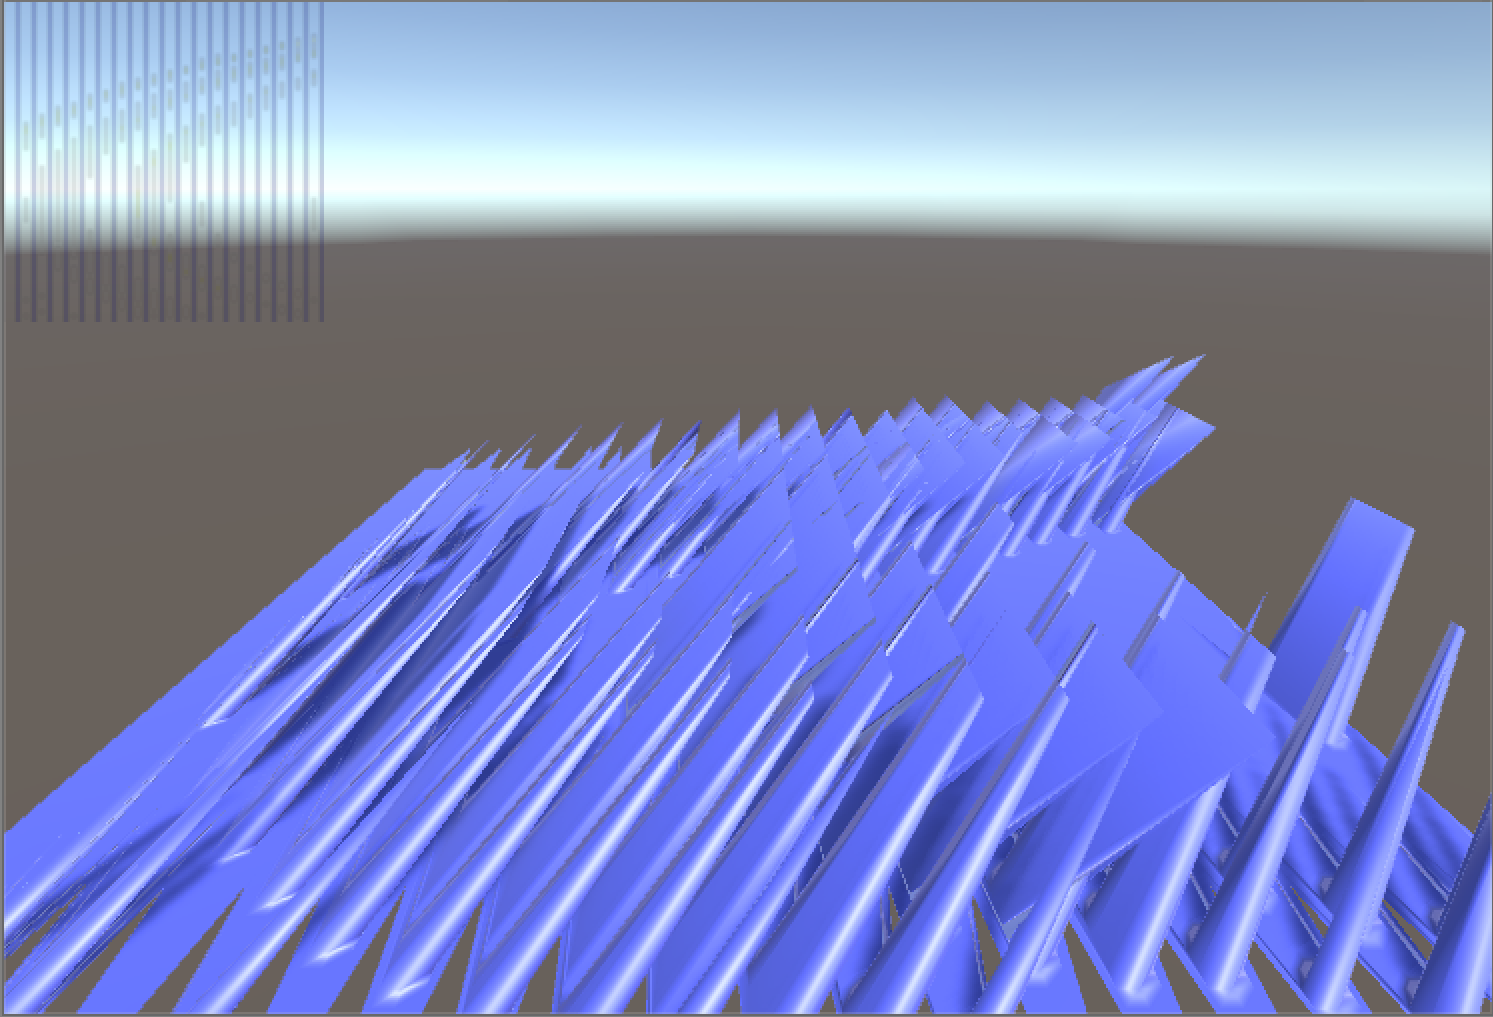
\includegraphics[width=0.8\linewidth]{texture_copy_issues}
\caption{An example of the issues that could be posed by shaders with no obvious
cause of error.}
\label{fig:texture_copy_issues}
\end{figure}

However, there were repeated causes of friction which added up over the course
of the project - most of which were a result of shader programming.

\subsection{Writing Shaders}

Writing shaders was an implementation challenge due to the immaturity of online
documentation and programming tools.

As most graphics programming is done in commercial environments, online
documentation was a lot more sparse than I expected. Furthermore, due to the
rapid development of GPUs, a lot of documentation mentioned features that were
out-of-date in non-obvious ways \cite{Yuksel2007} \cite{NoPointSpritesUnityOne}
\cite{NoPointSpritesWorkaround}.

Because no compile- or run-time checks were performed to check the validity
of data structures shared by the GPU and the CPU, the biggest challenge by far
was ensuring they were kept in-sync. This extended from maintaining the
coherency of data-structure definitions in both HLSL and C\#, to ensuring
strings identifying arguments for the GPU were spelled correctly on the CPU -
with no mechanisms to detect if any dependencies changed. Fortunately, I
managed to structure a step-by-step system which prevented this from causing a
major issue. However, it was completely unnecessary and has led me to be
interested in analysing this problem as a project in and of itself.

% POSSIBLE: mention how Unity documentation was lacking

\section{Success Criteria}

All the project requirements were met, barring part of one: I managed to create
a Wave Particle simulation in Unity that ran on both the CPU and GPU. However,
even though I implemented a basic fluid-object interaction system, I only did
so for the GPU (Figure \ref{fig:cube_drag_1}).

\begin{figure}[h]
\centering
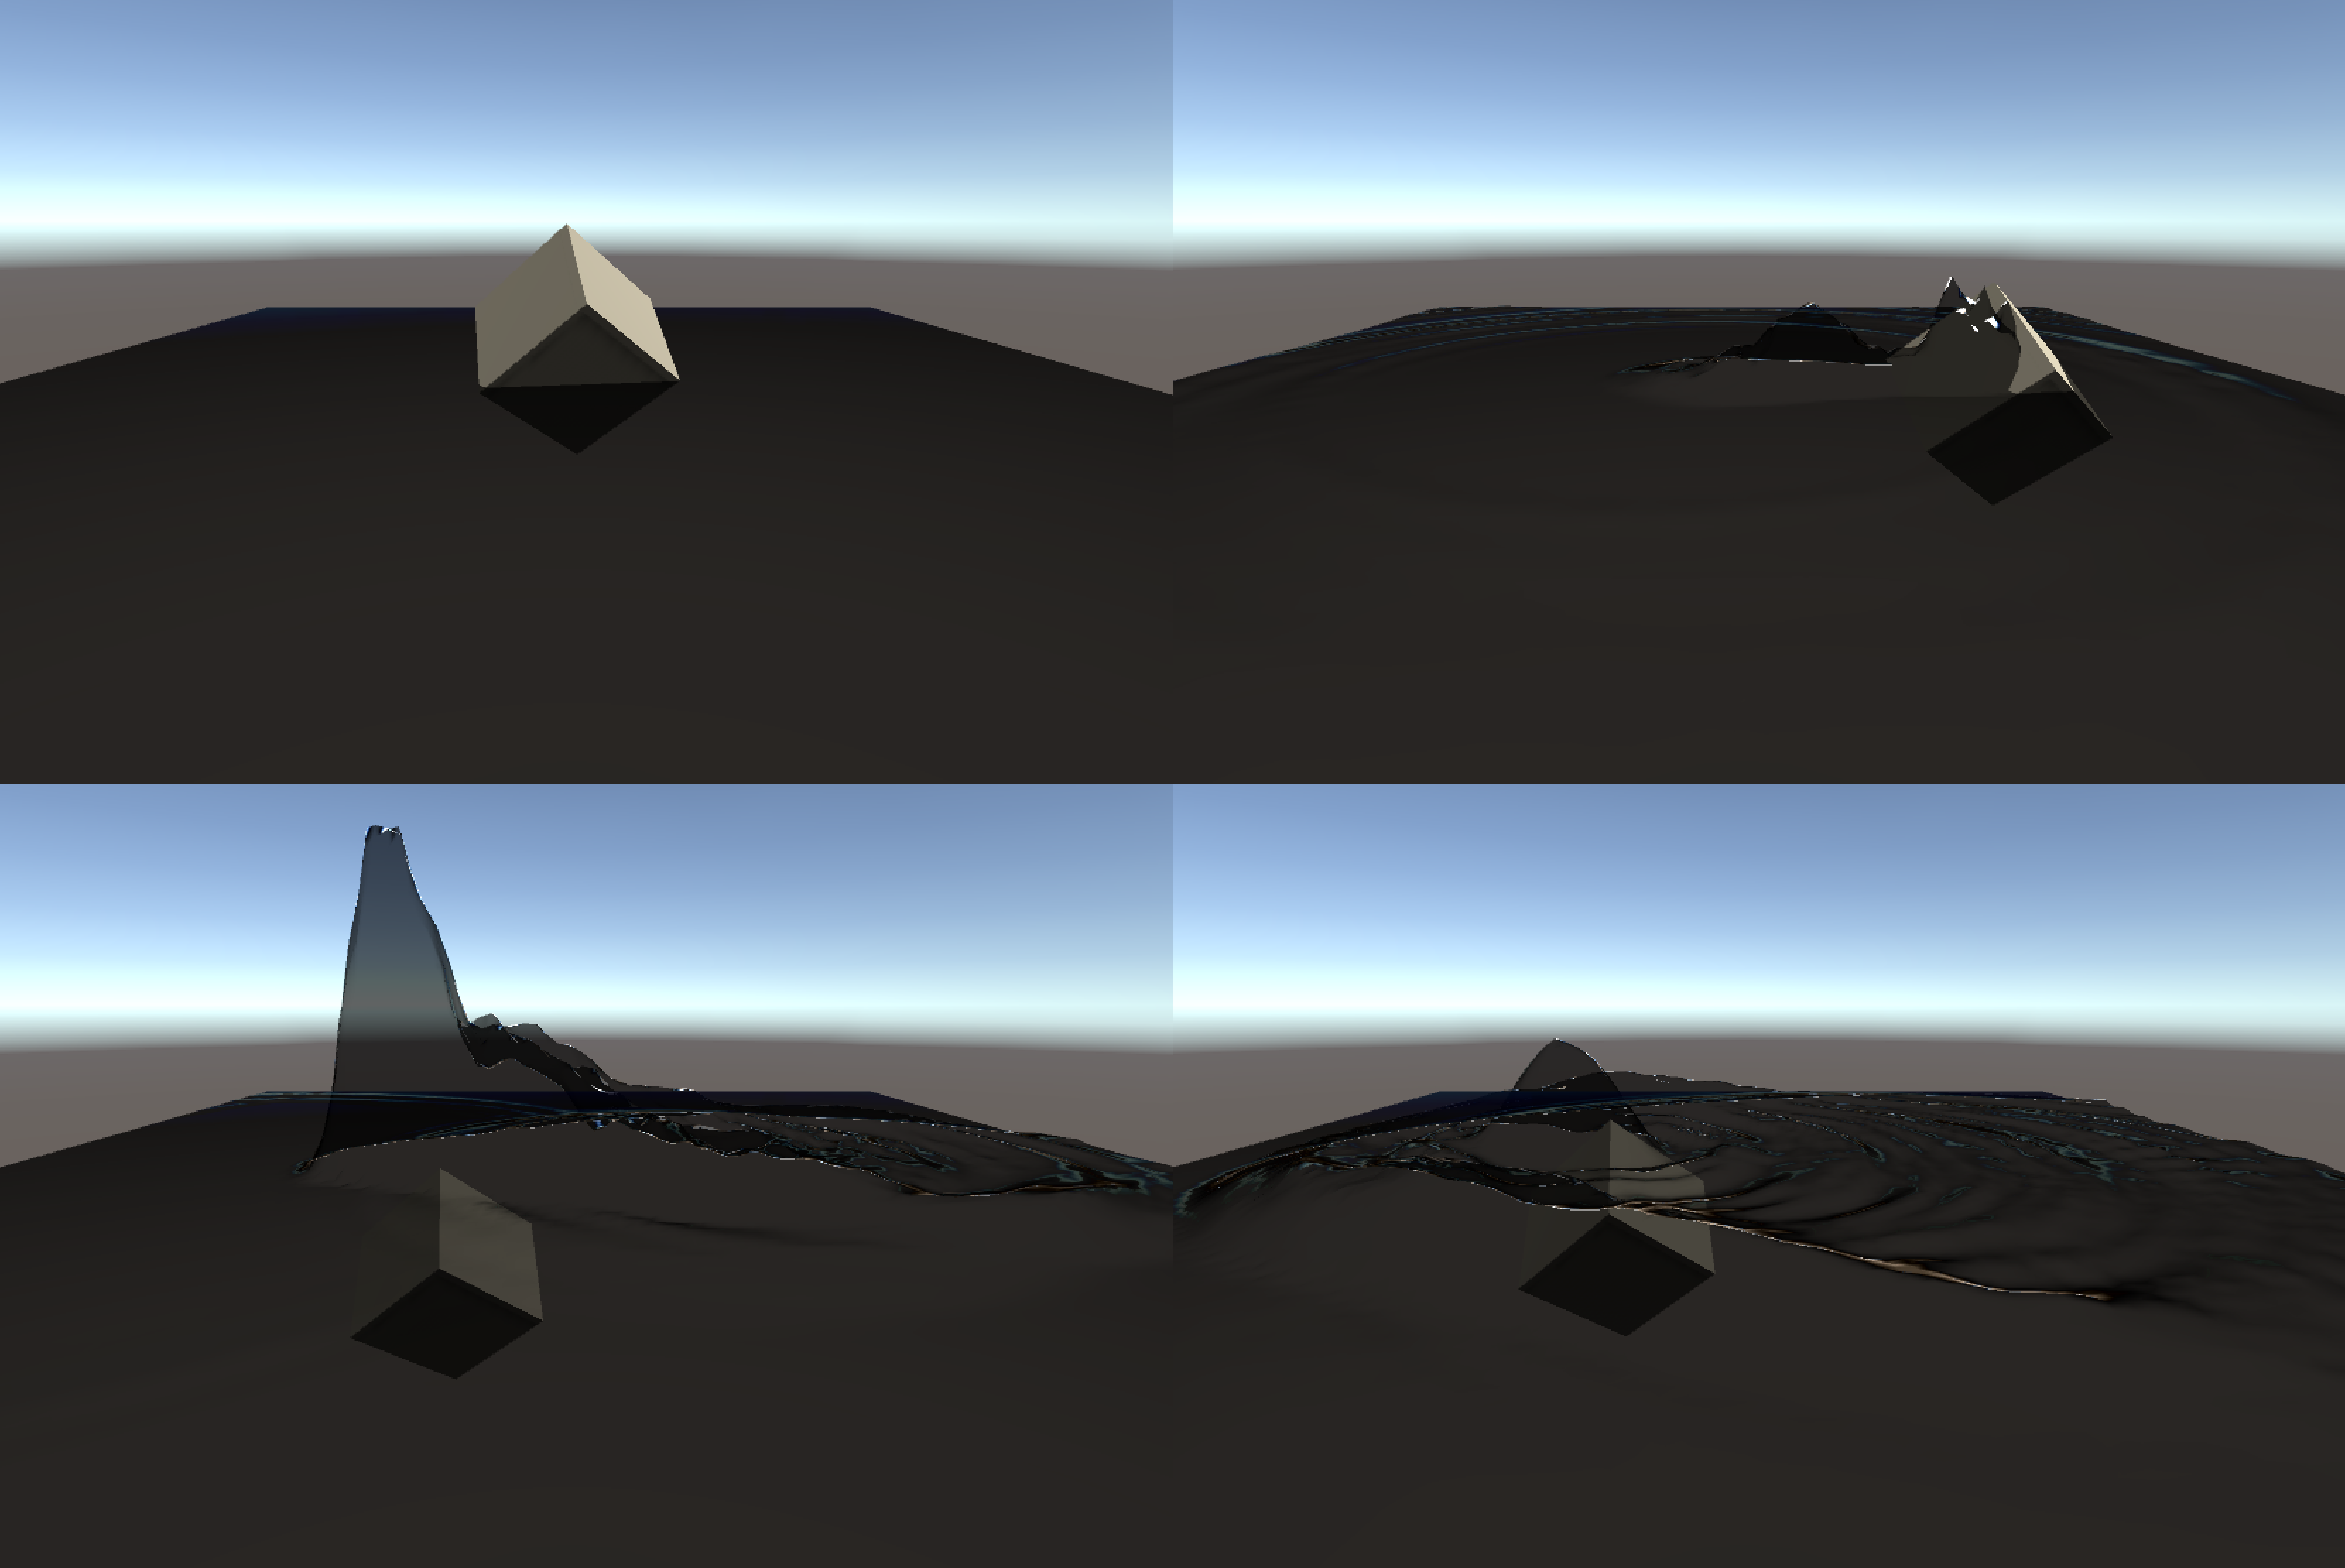
\includegraphics[width=0.8\linewidth]{cube_drag_all}
\caption{Showing the effects of dragging a cube through the water. From top
left going clockwise: cube in initial position, then being dragged to the
right, then being dragged to the left, then finally floating the surface after
being left to rest.}
\label{fig:cube_drag_1}
\end{figure}

I achieved the goal of a GPU-based version of the simulation that ran at least
30 frames-per-second with 5000 Wave Particles present. In fact, framerates of
60 frames-per-second were achievable with 5,000,000 Wave Particles present. A
500-fold increase over the 10,000 particles at 60 frames-per-second in the
original Wave Particles paper \cite{Yuksel2007}, despite only a 5-to-10-fold
increase in effective computing power over the \textit{Nvidia GeForce 7900 GTX}
used in the original paper \cite{GPUComparison}.

Figure \ref{fig:wave_particles_gui} demonstrates my implementation of a
two-dimensional top-down overlay-visualiser of the system to enable easy
visualisation, for both explanatory and debugging purposes. Furthermore, a
basic water renderer for the wavefronts generated by Wave Particles was
completed, in addition to the extension of implementing the Fresnel effect.

% POSSIBLE: Put this on YouTube?

\begin{figure}[h]
\centering
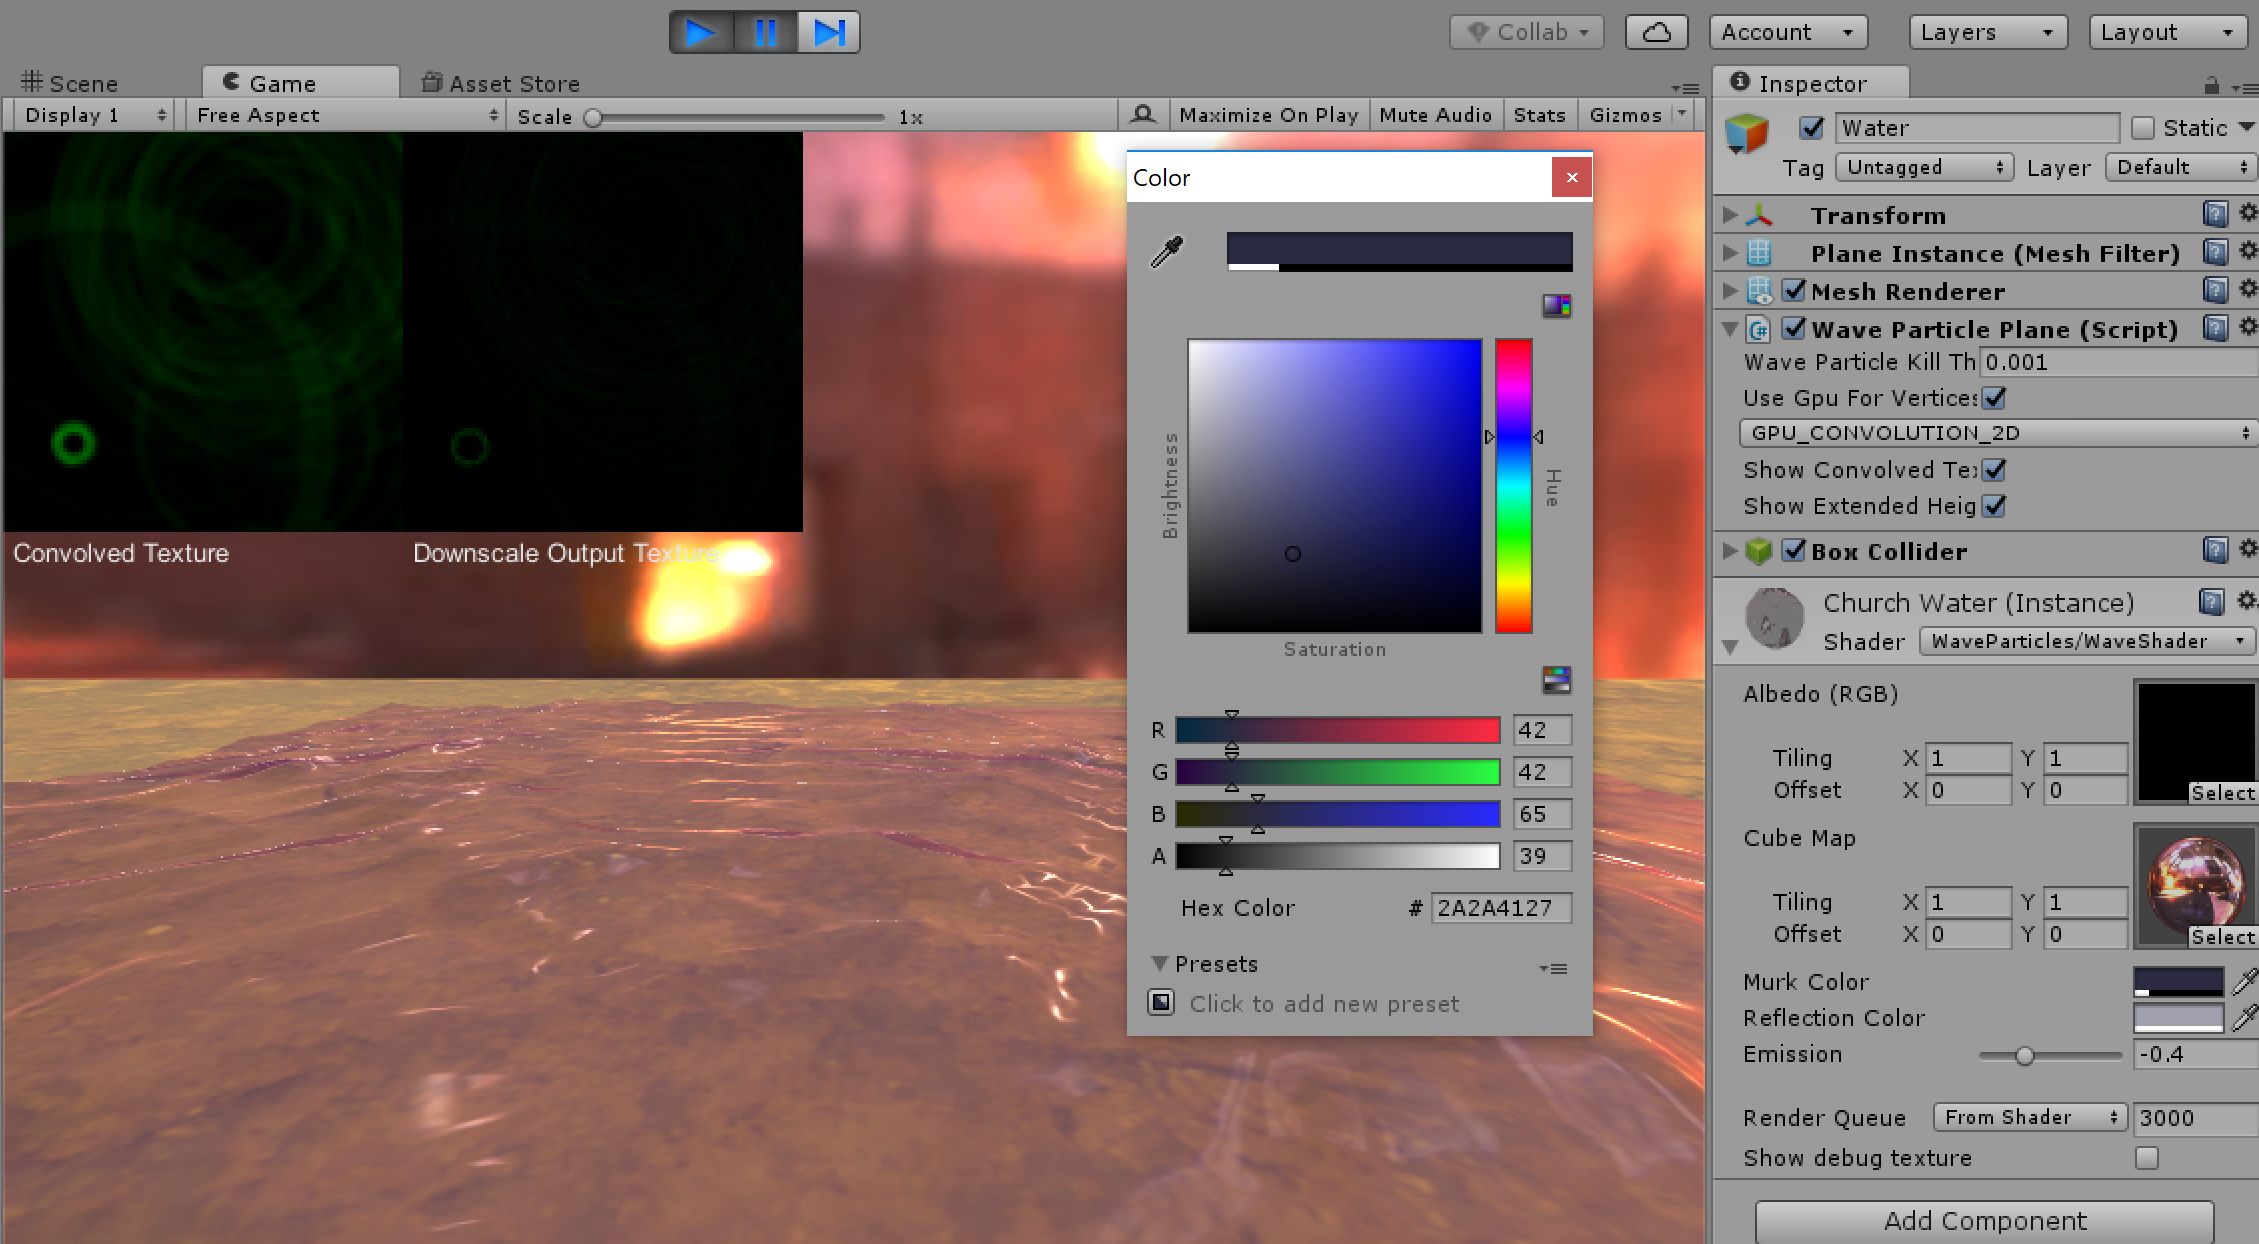
\includegraphics[width=0.8\linewidth]{wave_particles_gui}
\caption{My Wave Particles implementation within Unity, demonstrating a variety
of features. The overlay-visualiser is shown in the top-left. Furthermore, the
ability to dynamically change the reflectivity of the water via color-selection
is shown. Finally, on the right it can be seen how implementations of different
aspects of the system can be changed at run-time within the editor.}
\label{fig:wave_particles_gui}
\end{figure}

I wrote a system to manage the Wave Particles and object placement within the
Unity editor. This system has the ability to let users choose which
implementation of different parts of the pipeline are used. Furthermore, I let
users modify parameters of the system - including the kill threshold, the color
of the water, the water's transparency and its reflectivity (Figure
\ref{fig:wave_particles_gui}).

Additionally, I completed measurements comparing the performance of the CPU-
and GPU-based implementations of specific features and how the number of Wave
Particles affected the performance of the simulation.

Finally, I enabled Virtual Reality using an Oculus Rift DK2 - which was
extremely straightforward using Unity's native support.
%TODO: Add Figure

\section{Summary}

I analysed and compared the performance and memory usage of all the different
implementations of various parts of the Wave Particles pipeline. Furthermore, I
looked at how resource usage scaled as various parameters changed - in
particular how the number of active particles and the resolution of the
displacement map affected runtime factors. I then discussed some of the
challenges faced before evaluating whether the project requirements were
successfully met.

\chapter{Conclusions}

% POSSIBLE: possibly mention how in hindsight it may have been better to choose a
% different option?

In this project I set out to implement the Wave Particles system for animating
sufficiently realistic water waves in real-time on the GPU and CPU on top of
the Unity game engine. Furthermore, the goal was to optimise the system, and
compare the GPU and CPU implementations to show the performance improvements
GPUs can achieve.

I have achieved my main goals, not just showing that the system can run at
least at 30 FPS with 5000 Wave Particles on a laptop GPU - but managing a
500-fold performance increase with only a 5-to-10 fold increase in computing
power over the 10,000 Wave Particles at 60 FPS in the original paper by using a
novel GPU data-structure \cite{Yuksel2007}. I also completed two extensions,
implementing realistic reflections on the GPU using cubemaps and enabling the
system in VR. The latter was straight-forward and highlighted one of the
benefits of using a commercial game engine.

Personally, I also wanted to learn about graphics programming, especially as
the performance gains it can offer over CPU programs in parallel computation can
be staggering. I was successful in doing so and the potential benefits of GPU
programming have been confirmed. However, having learnt so much about the
subject matter, game engines and graphics programming, I would do some things
differently in hindsight.

If I were to do the project again, I would not place such a heavy focus on
comparing the performance of different implementations - specifically across
the CPU and GPU. I would have oriented my project around implementing the core
on the GPU, leaving more time, room and flexibility to complete some of the
extension ideas I had.

% POSSIBLE: expand

In implementing and expanding on Wave Particles, I have built a system which
has a lot of potential in real-time rendering. The project still excites me and
I plan on expanding it beyond its purpose as a Part II project going forward.

\section{Future Extensions}
\label{sec:future_extensions}

There are many possible directions this project could be taken in. In this
section I describe some of the ideas I had but couldn't complete.

\subsection{Signed Distance Field Reflections}

Reflecting Wave Particles is incredibly limited and only works within a
rectangular bounded space. However, if there were a way to capture the shape of
static boundaries in a signed distance field - this could not only be used for
efficiently determining the location of Wave Particle reflections, but also for
encoding the shape of the boundaries such that the dispersion angle of Wave
Particles could be updated to match them.

\subsection{Dynamic Performance-Based Resolution Scaling of the Displacement Map}

The resolution of the displacement map affects the performance of the system
significantly. Many games use adaptive techniques to lower the resolution of
the frame-buffer when performance would otherwise suffer. This could
potentially be applied to the displacement map.

\subsection{Adaptable LoD system for Oceans}

Open oceans are large; having an LoD (Level of Detail) system of different
\textit{patches} of Wave Particles could be used in order to render boundless
seas.

\subsection{Planes of Multiple Frequencies}

Multiple planes of Wave Particles could be use to model water waves of
different frequencies.

\bibliographystyle{unsrt}

\bibliography{references}

\appendix

\chapter{TravisCI}
\label{app:travisci}

Script that automatically installs Unity.

\begin{lstlisting}[language=Bash]
#! /bin/sh

# This program installs the version of Unity used to run this project in Travis CI

UNITY_VERSION='5.5.1f1'
# Use http://unity3d.com/get-unity/download/archive for up-to-date Unity links
DOWNLOAD_LOCATION='http://netstorage.unity3d.com/unity/88d00a7498cd/MacEditorInstaller/Unity-'"$UNITY_VERSION"'.pkg'
FILE_NAME='unity.pkg'

echo "Downloading Unity from $DOWNLOAD_LOCATION to $FILE_NAME"
curl -o Unity.pkg $DOWNLOAD_LOCATION

echo "Installing Unity from $FILE_NAME"
sudo installer -dumplog -package $FILE_NAME -target /
\end{lstlisting}

Script that automatically runs all Unity unit tests.

\begin{lstlisting}[language=Bash]
#! /bin/bash
ROOT_PROJECT_PATH="$TRAVIS_BUILD_DIR"

UNITY_LOCATION='/Applications/Unity/Unity.app/Contents/MacOS/Unity'
PROJECT_PATH=$ROOT_PROJECT_PATH'/project/Wave Particles'
RESULT_LOCATION=$ROOT_PROJECT_PATH

echo "Calling Unit Test script..."
echo 'source ./scripts/runTests.sh' "$UNITY_LOCATION" "$PROJECT_PATH" "$RESULT_LOCATION"
source ./scripts/runTests.sh "$UNITY_LOCATION" "$PROJECT_PATH" "$RESULT_LOCATION" python3
\end{lstlisting}

\chapter{Convolution Shader}
\label{app:convolution_shader}

The script below shows the shader that was used when convolving Wave Particles. 
\begin{lstlisting}[language=C]
sampler2D _MainTex;
sampler2D _KernelTex;
float4 _MainTex_ST;
float _HoriRes;
float _VertRes;
float _Width;
float _Height;
float _ParticleRadii;

fixed4 frag(v2f i) : SV_Target
{
    //// sample the texture
    const float unitX = _Width / _HoriRes;
    const float unitY = _Height / _VertRes;

    float4 color = float4(0, 0, 0, 1);

    for (float x = 0; x < _KernelWidth; x++) {
        for (float y = 0; y < _KernelHeight; y++) {
            float2 coords = i.uv + float2((x - (_KernelWidth * 0.5))/ _HoriRes, (y - (_KernelHeight * 0.5)) / _VertRes);
            float4 newVal = tex2D(_MainTex, coords);
            float4 kernelColor = tex2D(_KernelTex, float2(x / _KernelWidth, y / _KernelHeight));
            color += newVal.g * kernelColor;
        }
    }

    return color;
}
\end{lstlisting}

\chapter{Performance Graphs}

\section{Splatting Wave Particles}
\label{app:performance_graphs_splatting}

The graphs below were profiled under the following conditions:

There were $0$ active Wave Particles in the first frame, every frame a new Wave
Particle was generated with an amplitude of $0.8m$ and a dispersion angle of
$2\pi$. The particles were set with a radius of $0.2m$ and a speed of
$1ms^{-1}$. Finally, the plane had a width and height of $8m$ and resolution of
100 by 100 pixels/vertices.

\begin{figure}[H]
\centering
%% Creator: Matplotlib, PGF backend
%%
%% To include the figure in your LaTeX document, write
%%   \input{<filename>.pgf}
%%
%% Make sure the required packages are loaded in your preamble
%%   \usepackage{pgf}
%%
%% Figures using additional raster images can only be included by \input if
%% they are in the same directory as the main LaTeX file. For loading figures
%% from other directories you can use the `import` package
%%   \usepackage{import}
%% and then include the figures with
%%   \import{<path to file>}{<filename>.pgf}
%%
%% Matplotlib used the following preamble
%%   \usepackage{fontspec}
%%
\begingroup%
\makeatletter%
\begin{pgfpicture}%
\pgfpathrectangle{\pgfpointorigin}{\pgfqpoint{6.400000in}{4.800000in}}%
\pgfusepath{use as bounding box, clip}%
\begin{pgfscope}%
\pgfsetbuttcap%
\pgfsetmiterjoin%
\definecolor{currentfill}{rgb}{1.000000,1.000000,1.000000}%
\pgfsetfillcolor{currentfill}%
\pgfsetlinewidth{0.000000pt}%
\definecolor{currentstroke}{rgb}{1.000000,1.000000,1.000000}%
\pgfsetstrokecolor{currentstroke}%
\pgfsetdash{}{0pt}%
\pgfpathmoveto{\pgfqpoint{0.000000in}{0.000000in}}%
\pgfpathlineto{\pgfqpoint{6.400000in}{0.000000in}}%
\pgfpathlineto{\pgfqpoint{6.400000in}{4.800000in}}%
\pgfpathlineto{\pgfqpoint{0.000000in}{4.800000in}}%
\pgfpathclose%
\pgfusepath{fill}%
\end{pgfscope}%
\begin{pgfscope}%
\pgfsetbuttcap%
\pgfsetmiterjoin%
\definecolor{currentfill}{rgb}{0.898039,0.898039,0.898039}%
\pgfsetfillcolor{currentfill}%
\pgfsetlinewidth{0.000000pt}%
\definecolor{currentstroke}{rgb}{0.000000,0.000000,0.000000}%
\pgfsetstrokecolor{currentstroke}%
\pgfsetstrokeopacity{0.000000}%
\pgfsetdash{}{0pt}%
\pgfpathmoveto{\pgfqpoint{0.800000in}{0.528000in}}%
\pgfpathlineto{\pgfqpoint{5.760000in}{0.528000in}}%
\pgfpathlineto{\pgfqpoint{5.760000in}{4.224000in}}%
\pgfpathlineto{\pgfqpoint{0.800000in}{4.224000in}}%
\pgfpathclose%
\pgfusepath{fill}%
\end{pgfscope}%
\begin{pgfscope}%
\pgfpathrectangle{\pgfqpoint{0.800000in}{0.528000in}}{\pgfqpoint{4.960000in}{3.696000in}} %
\pgfusepath{clip}%
\pgfsetrectcap%
\pgfsetroundjoin%
\pgfsetlinewidth{0.803000pt}%
\definecolor{currentstroke}{rgb}{1.000000,1.000000,1.000000}%
\pgfsetstrokecolor{currentstroke}%
\pgfsetdash{}{0pt}%
\pgfpathmoveto{\pgfqpoint{0.800000in}{0.528000in}}%
\pgfpathlineto{\pgfqpoint{0.800000in}{4.224000in}}%
\pgfusepath{stroke}%
\end{pgfscope}%
\begin{pgfscope}%
\pgfsetbuttcap%
\pgfsetroundjoin%
\definecolor{currentfill}{rgb}{0.333333,0.333333,0.333333}%
\pgfsetfillcolor{currentfill}%
\pgfsetlinewidth{0.803000pt}%
\definecolor{currentstroke}{rgb}{0.333333,0.333333,0.333333}%
\pgfsetstrokecolor{currentstroke}%
\pgfsetdash{}{0pt}%
\pgfsys@defobject{currentmarker}{\pgfqpoint{0.000000in}{-0.048611in}}{\pgfqpoint{0.000000in}{0.000000in}}{%
\pgfpathmoveto{\pgfqpoint{0.000000in}{0.000000in}}%
\pgfpathlineto{\pgfqpoint{0.000000in}{-0.048611in}}%
\pgfusepath{stroke,fill}%
}%
\begin{pgfscope}%
\pgfsys@transformshift{0.800000in}{0.528000in}%
\pgfsys@useobject{currentmarker}{}%
\end{pgfscope}%
\end{pgfscope}%
\begin{pgfscope}%
\definecolor{textcolor}{rgb}{0.333333,0.333333,0.333333}%
\pgfsetstrokecolor{textcolor}%
\pgfsetfillcolor{textcolor}%
\pgftext[x=0.800000in,y=0.430778in,,top]{\color{textcolor}\rmfamily\fontsize{10.000000}{12.000000}\selectfont \(\displaystyle 0\)}%
\end{pgfscope}%
\begin{pgfscope}%
\pgfpathrectangle{\pgfqpoint{0.800000in}{0.528000in}}{\pgfqpoint{4.960000in}{3.696000in}} %
\pgfusepath{clip}%
\pgfsetrectcap%
\pgfsetroundjoin%
\pgfsetlinewidth{0.803000pt}%
\definecolor{currentstroke}{rgb}{1.000000,1.000000,1.000000}%
\pgfsetstrokecolor{currentstroke}%
\pgfsetdash{}{0pt}%
\pgfpathmoveto{\pgfqpoint{1.629431in}{0.528000in}}%
\pgfpathlineto{\pgfqpoint{1.629431in}{4.224000in}}%
\pgfusepath{stroke}%
\end{pgfscope}%
\begin{pgfscope}%
\pgfsetbuttcap%
\pgfsetroundjoin%
\definecolor{currentfill}{rgb}{0.333333,0.333333,0.333333}%
\pgfsetfillcolor{currentfill}%
\pgfsetlinewidth{0.803000pt}%
\definecolor{currentstroke}{rgb}{0.333333,0.333333,0.333333}%
\pgfsetstrokecolor{currentstroke}%
\pgfsetdash{}{0pt}%
\pgfsys@defobject{currentmarker}{\pgfqpoint{0.000000in}{-0.048611in}}{\pgfqpoint{0.000000in}{0.000000in}}{%
\pgfpathmoveto{\pgfqpoint{0.000000in}{0.000000in}}%
\pgfpathlineto{\pgfqpoint{0.000000in}{-0.048611in}}%
\pgfusepath{stroke,fill}%
}%
\begin{pgfscope}%
\pgfsys@transformshift{1.629431in}{0.528000in}%
\pgfsys@useobject{currentmarker}{}%
\end{pgfscope}%
\end{pgfscope}%
\begin{pgfscope}%
\definecolor{textcolor}{rgb}{0.333333,0.333333,0.333333}%
\pgfsetstrokecolor{textcolor}%
\pgfsetfillcolor{textcolor}%
\pgftext[x=1.629431in,y=0.430778in,,top]{\color{textcolor}\rmfamily\fontsize{10.000000}{12.000000}\selectfont \(\displaystyle 50\)}%
\end{pgfscope}%
\begin{pgfscope}%
\pgfpathrectangle{\pgfqpoint{0.800000in}{0.528000in}}{\pgfqpoint{4.960000in}{3.696000in}} %
\pgfusepath{clip}%
\pgfsetrectcap%
\pgfsetroundjoin%
\pgfsetlinewidth{0.803000pt}%
\definecolor{currentstroke}{rgb}{1.000000,1.000000,1.000000}%
\pgfsetstrokecolor{currentstroke}%
\pgfsetdash{}{0pt}%
\pgfpathmoveto{\pgfqpoint{2.458863in}{0.528000in}}%
\pgfpathlineto{\pgfqpoint{2.458863in}{4.224000in}}%
\pgfusepath{stroke}%
\end{pgfscope}%
\begin{pgfscope}%
\pgfsetbuttcap%
\pgfsetroundjoin%
\definecolor{currentfill}{rgb}{0.333333,0.333333,0.333333}%
\pgfsetfillcolor{currentfill}%
\pgfsetlinewidth{0.803000pt}%
\definecolor{currentstroke}{rgb}{0.333333,0.333333,0.333333}%
\pgfsetstrokecolor{currentstroke}%
\pgfsetdash{}{0pt}%
\pgfsys@defobject{currentmarker}{\pgfqpoint{0.000000in}{-0.048611in}}{\pgfqpoint{0.000000in}{0.000000in}}{%
\pgfpathmoveto{\pgfqpoint{0.000000in}{0.000000in}}%
\pgfpathlineto{\pgfqpoint{0.000000in}{-0.048611in}}%
\pgfusepath{stroke,fill}%
}%
\begin{pgfscope}%
\pgfsys@transformshift{2.458863in}{0.528000in}%
\pgfsys@useobject{currentmarker}{}%
\end{pgfscope}%
\end{pgfscope}%
\begin{pgfscope}%
\definecolor{textcolor}{rgb}{0.333333,0.333333,0.333333}%
\pgfsetstrokecolor{textcolor}%
\pgfsetfillcolor{textcolor}%
\pgftext[x=2.458863in,y=0.430778in,,top]{\color{textcolor}\rmfamily\fontsize{10.000000}{12.000000}\selectfont \(\displaystyle 100\)}%
\end{pgfscope}%
\begin{pgfscope}%
\pgfpathrectangle{\pgfqpoint{0.800000in}{0.528000in}}{\pgfqpoint{4.960000in}{3.696000in}} %
\pgfusepath{clip}%
\pgfsetrectcap%
\pgfsetroundjoin%
\pgfsetlinewidth{0.803000pt}%
\definecolor{currentstroke}{rgb}{1.000000,1.000000,1.000000}%
\pgfsetstrokecolor{currentstroke}%
\pgfsetdash{}{0pt}%
\pgfpathmoveto{\pgfqpoint{3.288294in}{0.528000in}}%
\pgfpathlineto{\pgfqpoint{3.288294in}{4.224000in}}%
\pgfusepath{stroke}%
\end{pgfscope}%
\begin{pgfscope}%
\pgfsetbuttcap%
\pgfsetroundjoin%
\definecolor{currentfill}{rgb}{0.333333,0.333333,0.333333}%
\pgfsetfillcolor{currentfill}%
\pgfsetlinewidth{0.803000pt}%
\definecolor{currentstroke}{rgb}{0.333333,0.333333,0.333333}%
\pgfsetstrokecolor{currentstroke}%
\pgfsetdash{}{0pt}%
\pgfsys@defobject{currentmarker}{\pgfqpoint{0.000000in}{-0.048611in}}{\pgfqpoint{0.000000in}{0.000000in}}{%
\pgfpathmoveto{\pgfqpoint{0.000000in}{0.000000in}}%
\pgfpathlineto{\pgfqpoint{0.000000in}{-0.048611in}}%
\pgfusepath{stroke,fill}%
}%
\begin{pgfscope}%
\pgfsys@transformshift{3.288294in}{0.528000in}%
\pgfsys@useobject{currentmarker}{}%
\end{pgfscope}%
\end{pgfscope}%
\begin{pgfscope}%
\definecolor{textcolor}{rgb}{0.333333,0.333333,0.333333}%
\pgfsetstrokecolor{textcolor}%
\pgfsetfillcolor{textcolor}%
\pgftext[x=3.288294in,y=0.430778in,,top]{\color{textcolor}\rmfamily\fontsize{10.000000}{12.000000}\selectfont \(\displaystyle 150\)}%
\end{pgfscope}%
\begin{pgfscope}%
\pgfpathrectangle{\pgfqpoint{0.800000in}{0.528000in}}{\pgfqpoint{4.960000in}{3.696000in}} %
\pgfusepath{clip}%
\pgfsetrectcap%
\pgfsetroundjoin%
\pgfsetlinewidth{0.803000pt}%
\definecolor{currentstroke}{rgb}{1.000000,1.000000,1.000000}%
\pgfsetstrokecolor{currentstroke}%
\pgfsetdash{}{0pt}%
\pgfpathmoveto{\pgfqpoint{4.117726in}{0.528000in}}%
\pgfpathlineto{\pgfqpoint{4.117726in}{4.224000in}}%
\pgfusepath{stroke}%
\end{pgfscope}%
\begin{pgfscope}%
\pgfsetbuttcap%
\pgfsetroundjoin%
\definecolor{currentfill}{rgb}{0.333333,0.333333,0.333333}%
\pgfsetfillcolor{currentfill}%
\pgfsetlinewidth{0.803000pt}%
\definecolor{currentstroke}{rgb}{0.333333,0.333333,0.333333}%
\pgfsetstrokecolor{currentstroke}%
\pgfsetdash{}{0pt}%
\pgfsys@defobject{currentmarker}{\pgfqpoint{0.000000in}{-0.048611in}}{\pgfqpoint{0.000000in}{0.000000in}}{%
\pgfpathmoveto{\pgfqpoint{0.000000in}{0.000000in}}%
\pgfpathlineto{\pgfqpoint{0.000000in}{-0.048611in}}%
\pgfusepath{stroke,fill}%
}%
\begin{pgfscope}%
\pgfsys@transformshift{4.117726in}{0.528000in}%
\pgfsys@useobject{currentmarker}{}%
\end{pgfscope}%
\end{pgfscope}%
\begin{pgfscope}%
\definecolor{textcolor}{rgb}{0.333333,0.333333,0.333333}%
\pgfsetstrokecolor{textcolor}%
\pgfsetfillcolor{textcolor}%
\pgftext[x=4.117726in,y=0.430778in,,top]{\color{textcolor}\rmfamily\fontsize{10.000000}{12.000000}\selectfont \(\displaystyle 200\)}%
\end{pgfscope}%
\begin{pgfscope}%
\pgfpathrectangle{\pgfqpoint{0.800000in}{0.528000in}}{\pgfqpoint{4.960000in}{3.696000in}} %
\pgfusepath{clip}%
\pgfsetrectcap%
\pgfsetroundjoin%
\pgfsetlinewidth{0.803000pt}%
\definecolor{currentstroke}{rgb}{1.000000,1.000000,1.000000}%
\pgfsetstrokecolor{currentstroke}%
\pgfsetdash{}{0pt}%
\pgfpathmoveto{\pgfqpoint{4.947157in}{0.528000in}}%
\pgfpathlineto{\pgfqpoint{4.947157in}{4.224000in}}%
\pgfusepath{stroke}%
\end{pgfscope}%
\begin{pgfscope}%
\pgfsetbuttcap%
\pgfsetroundjoin%
\definecolor{currentfill}{rgb}{0.333333,0.333333,0.333333}%
\pgfsetfillcolor{currentfill}%
\pgfsetlinewidth{0.803000pt}%
\definecolor{currentstroke}{rgb}{0.333333,0.333333,0.333333}%
\pgfsetstrokecolor{currentstroke}%
\pgfsetdash{}{0pt}%
\pgfsys@defobject{currentmarker}{\pgfqpoint{0.000000in}{-0.048611in}}{\pgfqpoint{0.000000in}{0.000000in}}{%
\pgfpathmoveto{\pgfqpoint{0.000000in}{0.000000in}}%
\pgfpathlineto{\pgfqpoint{0.000000in}{-0.048611in}}%
\pgfusepath{stroke,fill}%
}%
\begin{pgfscope}%
\pgfsys@transformshift{4.947157in}{0.528000in}%
\pgfsys@useobject{currentmarker}{}%
\end{pgfscope}%
\end{pgfscope}%
\begin{pgfscope}%
\definecolor{textcolor}{rgb}{0.333333,0.333333,0.333333}%
\pgfsetstrokecolor{textcolor}%
\pgfsetfillcolor{textcolor}%
\pgftext[x=4.947157in,y=0.430778in,,top]{\color{textcolor}\rmfamily\fontsize{10.000000}{12.000000}\selectfont \(\displaystyle 250\)}%
\end{pgfscope}%
\begin{pgfscope}%
\definecolor{textcolor}{rgb}{0.333333,0.333333,0.333333}%
\pgfsetstrokecolor{textcolor}%
\pgfsetfillcolor{textcolor}%
\pgftext[x=3.280000in,y=0.251889in,,top]{\color{textcolor}\rmfamily\fontsize{12.000000}{14.400000}\selectfont Frame Number}%
\end{pgfscope}%
\begin{pgfscope}%
\pgfpathrectangle{\pgfqpoint{0.800000in}{0.528000in}}{\pgfqpoint{4.960000in}{3.696000in}} %
\pgfusepath{clip}%
\pgfsetrectcap%
\pgfsetroundjoin%
\pgfsetlinewidth{0.803000pt}%
\definecolor{currentstroke}{rgb}{1.000000,1.000000,1.000000}%
\pgfsetstrokecolor{currentstroke}%
\pgfsetdash{}{0pt}%
\pgfpathmoveto{\pgfqpoint{0.800000in}{0.903123in}}%
\pgfpathlineto{\pgfqpoint{5.760000in}{0.903123in}}%
\pgfusepath{stroke}%
\end{pgfscope}%
\begin{pgfscope}%
\pgfsetbuttcap%
\pgfsetroundjoin%
\definecolor{currentfill}{rgb}{0.333333,0.333333,0.333333}%
\pgfsetfillcolor{currentfill}%
\pgfsetlinewidth{0.803000pt}%
\definecolor{currentstroke}{rgb}{0.333333,0.333333,0.333333}%
\pgfsetstrokecolor{currentstroke}%
\pgfsetdash{}{0pt}%
\pgfsys@defobject{currentmarker}{\pgfqpoint{-0.048611in}{0.000000in}}{\pgfqpoint{0.000000in}{0.000000in}}{%
\pgfpathmoveto{\pgfqpoint{0.000000in}{0.000000in}}%
\pgfpathlineto{\pgfqpoint{-0.048611in}{0.000000in}}%
\pgfusepath{stroke,fill}%
}%
\begin{pgfscope}%
\pgfsys@transformshift{0.800000in}{0.903123in}%
\pgfsys@useobject{currentmarker}{}%
\end{pgfscope}%
\end{pgfscope}%
\begin{pgfscope}%
\definecolor{textcolor}{rgb}{0.333333,0.333333,0.333333}%
\pgfsetstrokecolor{textcolor}%
\pgfsetfillcolor{textcolor}%
\pgftext[x=0.633333in,y=0.854929in,left,base]{\color{textcolor}\rmfamily\fontsize{10.000000}{12.000000}\selectfont \(\displaystyle 2\)}%
\end{pgfscope}%
\begin{pgfscope}%
\pgfpathrectangle{\pgfqpoint{0.800000in}{0.528000in}}{\pgfqpoint{4.960000in}{3.696000in}} %
\pgfusepath{clip}%
\pgfsetrectcap%
\pgfsetroundjoin%
\pgfsetlinewidth{0.803000pt}%
\definecolor{currentstroke}{rgb}{1.000000,1.000000,1.000000}%
\pgfsetstrokecolor{currentstroke}%
\pgfsetdash{}{0pt}%
\pgfpathmoveto{\pgfqpoint{0.800000in}{1.478466in}}%
\pgfpathlineto{\pgfqpoint{5.760000in}{1.478466in}}%
\pgfusepath{stroke}%
\end{pgfscope}%
\begin{pgfscope}%
\pgfsetbuttcap%
\pgfsetroundjoin%
\definecolor{currentfill}{rgb}{0.333333,0.333333,0.333333}%
\pgfsetfillcolor{currentfill}%
\pgfsetlinewidth{0.803000pt}%
\definecolor{currentstroke}{rgb}{0.333333,0.333333,0.333333}%
\pgfsetstrokecolor{currentstroke}%
\pgfsetdash{}{0pt}%
\pgfsys@defobject{currentmarker}{\pgfqpoint{-0.048611in}{0.000000in}}{\pgfqpoint{0.000000in}{0.000000in}}{%
\pgfpathmoveto{\pgfqpoint{0.000000in}{0.000000in}}%
\pgfpathlineto{\pgfqpoint{-0.048611in}{0.000000in}}%
\pgfusepath{stroke,fill}%
}%
\begin{pgfscope}%
\pgfsys@transformshift{0.800000in}{1.478466in}%
\pgfsys@useobject{currentmarker}{}%
\end{pgfscope}%
\end{pgfscope}%
\begin{pgfscope}%
\definecolor{textcolor}{rgb}{0.333333,0.333333,0.333333}%
\pgfsetstrokecolor{textcolor}%
\pgfsetfillcolor{textcolor}%
\pgftext[x=0.633333in,y=1.430271in,left,base]{\color{textcolor}\rmfamily\fontsize{10.000000}{12.000000}\selectfont \(\displaystyle 4\)}%
\end{pgfscope}%
\begin{pgfscope}%
\pgfpathrectangle{\pgfqpoint{0.800000in}{0.528000in}}{\pgfqpoint{4.960000in}{3.696000in}} %
\pgfusepath{clip}%
\pgfsetrectcap%
\pgfsetroundjoin%
\pgfsetlinewidth{0.803000pt}%
\definecolor{currentstroke}{rgb}{1.000000,1.000000,1.000000}%
\pgfsetstrokecolor{currentstroke}%
\pgfsetdash{}{0pt}%
\pgfpathmoveto{\pgfqpoint{0.800000in}{2.053808in}}%
\pgfpathlineto{\pgfqpoint{5.760000in}{2.053808in}}%
\pgfusepath{stroke}%
\end{pgfscope}%
\begin{pgfscope}%
\pgfsetbuttcap%
\pgfsetroundjoin%
\definecolor{currentfill}{rgb}{0.333333,0.333333,0.333333}%
\pgfsetfillcolor{currentfill}%
\pgfsetlinewidth{0.803000pt}%
\definecolor{currentstroke}{rgb}{0.333333,0.333333,0.333333}%
\pgfsetstrokecolor{currentstroke}%
\pgfsetdash{}{0pt}%
\pgfsys@defobject{currentmarker}{\pgfqpoint{-0.048611in}{0.000000in}}{\pgfqpoint{0.000000in}{0.000000in}}{%
\pgfpathmoveto{\pgfqpoint{0.000000in}{0.000000in}}%
\pgfpathlineto{\pgfqpoint{-0.048611in}{0.000000in}}%
\pgfusepath{stroke,fill}%
}%
\begin{pgfscope}%
\pgfsys@transformshift{0.800000in}{2.053808in}%
\pgfsys@useobject{currentmarker}{}%
\end{pgfscope}%
\end{pgfscope}%
\begin{pgfscope}%
\definecolor{textcolor}{rgb}{0.333333,0.333333,0.333333}%
\pgfsetstrokecolor{textcolor}%
\pgfsetfillcolor{textcolor}%
\pgftext[x=0.633333in,y=2.005614in,left,base]{\color{textcolor}\rmfamily\fontsize{10.000000}{12.000000}\selectfont \(\displaystyle 6\)}%
\end{pgfscope}%
\begin{pgfscope}%
\pgfpathrectangle{\pgfqpoint{0.800000in}{0.528000in}}{\pgfqpoint{4.960000in}{3.696000in}} %
\pgfusepath{clip}%
\pgfsetrectcap%
\pgfsetroundjoin%
\pgfsetlinewidth{0.803000pt}%
\definecolor{currentstroke}{rgb}{1.000000,1.000000,1.000000}%
\pgfsetstrokecolor{currentstroke}%
\pgfsetdash{}{0pt}%
\pgfpathmoveto{\pgfqpoint{0.800000in}{2.629151in}}%
\pgfpathlineto{\pgfqpoint{5.760000in}{2.629151in}}%
\pgfusepath{stroke}%
\end{pgfscope}%
\begin{pgfscope}%
\pgfsetbuttcap%
\pgfsetroundjoin%
\definecolor{currentfill}{rgb}{0.333333,0.333333,0.333333}%
\pgfsetfillcolor{currentfill}%
\pgfsetlinewidth{0.803000pt}%
\definecolor{currentstroke}{rgb}{0.333333,0.333333,0.333333}%
\pgfsetstrokecolor{currentstroke}%
\pgfsetdash{}{0pt}%
\pgfsys@defobject{currentmarker}{\pgfqpoint{-0.048611in}{0.000000in}}{\pgfqpoint{0.000000in}{0.000000in}}{%
\pgfpathmoveto{\pgfqpoint{0.000000in}{0.000000in}}%
\pgfpathlineto{\pgfqpoint{-0.048611in}{0.000000in}}%
\pgfusepath{stroke,fill}%
}%
\begin{pgfscope}%
\pgfsys@transformshift{0.800000in}{2.629151in}%
\pgfsys@useobject{currentmarker}{}%
\end{pgfscope}%
\end{pgfscope}%
\begin{pgfscope}%
\definecolor{textcolor}{rgb}{0.333333,0.333333,0.333333}%
\pgfsetstrokecolor{textcolor}%
\pgfsetfillcolor{textcolor}%
\pgftext[x=0.633333in,y=2.580956in,left,base]{\color{textcolor}\rmfamily\fontsize{10.000000}{12.000000}\selectfont \(\displaystyle 8\)}%
\end{pgfscope}%
\begin{pgfscope}%
\pgfpathrectangle{\pgfqpoint{0.800000in}{0.528000in}}{\pgfqpoint{4.960000in}{3.696000in}} %
\pgfusepath{clip}%
\pgfsetrectcap%
\pgfsetroundjoin%
\pgfsetlinewidth{0.803000pt}%
\definecolor{currentstroke}{rgb}{1.000000,1.000000,1.000000}%
\pgfsetstrokecolor{currentstroke}%
\pgfsetdash{}{0pt}%
\pgfpathmoveto{\pgfqpoint{0.800000in}{3.204493in}}%
\pgfpathlineto{\pgfqpoint{5.760000in}{3.204493in}}%
\pgfusepath{stroke}%
\end{pgfscope}%
\begin{pgfscope}%
\pgfsetbuttcap%
\pgfsetroundjoin%
\definecolor{currentfill}{rgb}{0.333333,0.333333,0.333333}%
\pgfsetfillcolor{currentfill}%
\pgfsetlinewidth{0.803000pt}%
\definecolor{currentstroke}{rgb}{0.333333,0.333333,0.333333}%
\pgfsetstrokecolor{currentstroke}%
\pgfsetdash{}{0pt}%
\pgfsys@defobject{currentmarker}{\pgfqpoint{-0.048611in}{0.000000in}}{\pgfqpoint{0.000000in}{0.000000in}}{%
\pgfpathmoveto{\pgfqpoint{0.000000in}{0.000000in}}%
\pgfpathlineto{\pgfqpoint{-0.048611in}{0.000000in}}%
\pgfusepath{stroke,fill}%
}%
\begin{pgfscope}%
\pgfsys@transformshift{0.800000in}{3.204493in}%
\pgfsys@useobject{currentmarker}{}%
\end{pgfscope}%
\end{pgfscope}%
\begin{pgfscope}%
\definecolor{textcolor}{rgb}{0.333333,0.333333,0.333333}%
\pgfsetstrokecolor{textcolor}%
\pgfsetfillcolor{textcolor}%
\pgftext[x=0.563888in,y=3.156299in,left,base]{\color{textcolor}\rmfamily\fontsize{10.000000}{12.000000}\selectfont \(\displaystyle 10\)}%
\end{pgfscope}%
\begin{pgfscope}%
\pgfpathrectangle{\pgfqpoint{0.800000in}{0.528000in}}{\pgfqpoint{4.960000in}{3.696000in}} %
\pgfusepath{clip}%
\pgfsetrectcap%
\pgfsetroundjoin%
\pgfsetlinewidth{0.803000pt}%
\definecolor{currentstroke}{rgb}{1.000000,1.000000,1.000000}%
\pgfsetstrokecolor{currentstroke}%
\pgfsetdash{}{0pt}%
\pgfpathmoveto{\pgfqpoint{0.800000in}{3.779836in}}%
\pgfpathlineto{\pgfqpoint{5.760000in}{3.779836in}}%
\pgfusepath{stroke}%
\end{pgfscope}%
\begin{pgfscope}%
\pgfsetbuttcap%
\pgfsetroundjoin%
\definecolor{currentfill}{rgb}{0.333333,0.333333,0.333333}%
\pgfsetfillcolor{currentfill}%
\pgfsetlinewidth{0.803000pt}%
\definecolor{currentstroke}{rgb}{0.333333,0.333333,0.333333}%
\pgfsetstrokecolor{currentstroke}%
\pgfsetdash{}{0pt}%
\pgfsys@defobject{currentmarker}{\pgfqpoint{-0.048611in}{0.000000in}}{\pgfqpoint{0.000000in}{0.000000in}}{%
\pgfpathmoveto{\pgfqpoint{0.000000in}{0.000000in}}%
\pgfpathlineto{\pgfqpoint{-0.048611in}{0.000000in}}%
\pgfusepath{stroke,fill}%
}%
\begin{pgfscope}%
\pgfsys@transformshift{0.800000in}{3.779836in}%
\pgfsys@useobject{currentmarker}{}%
\end{pgfscope}%
\end{pgfscope}%
\begin{pgfscope}%
\definecolor{textcolor}{rgb}{0.333333,0.333333,0.333333}%
\pgfsetstrokecolor{textcolor}%
\pgfsetfillcolor{textcolor}%
\pgftext[x=0.563888in,y=3.731641in,left,base]{\color{textcolor}\rmfamily\fontsize{10.000000}{12.000000}\selectfont \(\displaystyle 12\)}%
\end{pgfscope}%
\begin{pgfscope}%
\definecolor{textcolor}{rgb}{0.333333,0.333333,0.333333}%
\pgfsetstrokecolor{textcolor}%
\pgfsetfillcolor{textcolor}%
\pgftext[x=0.508333in,y=2.376000in,,bottom,rotate=90.000000]{\color{textcolor}\rmfamily\fontsize{12.000000}{14.400000}\selectfont Frame Time (ms)}%
\end{pgfscope}%
\begin{pgfscope}%
\pgfpathrectangle{\pgfqpoint{0.800000in}{0.528000in}}{\pgfqpoint{4.960000in}{3.696000in}} %
\pgfusepath{clip}%
\pgfsetrectcap%
\pgfsetroundjoin%
\pgfsetlinewidth{1.505625pt}%
\definecolor{currentstroke}{rgb}{0.886275,0.290196,0.200000}%
\pgfsetstrokecolor{currentstroke}%
\pgfsetdash{}{0pt}%
\pgfpathmoveto{\pgfqpoint{0.800000in}{1.642438in}}%
\pgfpathlineto{\pgfqpoint{0.816589in}{1.763260in}}%
\pgfpathlineto{\pgfqpoint{0.833177in}{1.708603in}}%
\pgfpathlineto{\pgfqpoint{0.849766in}{1.722986in}}%
\pgfpathlineto{\pgfqpoint{0.866355in}{1.792027in}}%
\pgfpathlineto{\pgfqpoint{0.882943in}{1.820795in}}%
\pgfpathlineto{\pgfqpoint{0.899532in}{1.783397in}}%
\pgfpathlineto{\pgfqpoint{0.916120in}{1.875452in}}%
\pgfpathlineto{\pgfqpoint{0.932709in}{1.984767in}}%
\pgfpathlineto{\pgfqpoint{0.949298in}{2.076822in}}%
\pgfpathlineto{\pgfqpoint{0.965886in}{1.889836in}}%
\pgfpathlineto{\pgfqpoint{0.982475in}{1.979014in}}%
\pgfpathlineto{\pgfqpoint{0.999064in}{1.935863in}}%
\pgfpathlineto{\pgfqpoint{1.015652in}{1.990521in}}%
\pgfpathlineto{\pgfqpoint{1.032241in}{2.010658in}}%
\pgfpathlineto{\pgfqpoint{1.048829in}{1.961753in}}%
\pgfpathlineto{\pgfqpoint{1.065418in}{2.042301in}}%
\pgfpathlineto{\pgfqpoint{1.082007in}{2.065315in}}%
\pgfpathlineto{\pgfqpoint{1.098595in}{2.151616in}}%
\pgfpathlineto{\pgfqpoint{1.115184in}{2.361616in}}%
\pgfpathlineto{\pgfqpoint{1.131773in}{2.183260in}}%
\pgfpathlineto{\pgfqpoint{1.148361in}{2.235041in}}%
\pgfpathlineto{\pgfqpoint{1.164950in}{2.341479in}}%
\pgfpathlineto{\pgfqpoint{1.181538in}{2.462301in}}%
\pgfpathlineto{\pgfqpoint{1.198127in}{2.433534in}}%
\pgfpathlineto{\pgfqpoint{1.214716in}{2.588877in}}%
\pgfpathlineto{\pgfqpoint{1.231304in}{2.646411in}}%
\pgfpathlineto{\pgfqpoint{1.247893in}{2.850658in}}%
\pgfpathlineto{\pgfqpoint{1.264482in}{2.847781in}}%
\pgfpathlineto{\pgfqpoint{1.281070in}{2.902438in}}%
\pgfpathlineto{\pgfqpoint{1.297659in}{2.770110in}}%
\pgfpathlineto{\pgfqpoint{1.314247in}{2.934082in}}%
\pgfpathlineto{\pgfqpoint{1.330836in}{2.968603in}}%
\pgfpathlineto{\pgfqpoint{1.347425in}{2.939836in}}%
\pgfpathlineto{\pgfqpoint{1.364013in}{3.241890in}}%
\pgfpathlineto{\pgfqpoint{1.380602in}{3.394356in}}%
\pgfpathlineto{\pgfqpoint{1.397191in}{3.008877in}}%
\pgfpathlineto{\pgfqpoint{1.413779in}{3.011753in}}%
\pgfpathlineto{\pgfqpoint{1.430368in}{3.103808in}}%
\pgfpathlineto{\pgfqpoint{1.446957in}{3.040521in}}%
\pgfpathlineto{\pgfqpoint{1.463545in}{3.026137in}}%
\pgfpathlineto{\pgfqpoint{1.496722in}{3.138329in}}%
\pgfpathlineto{\pgfqpoint{1.513311in}{4.027233in}}%
\pgfpathlineto{\pgfqpoint{1.529900in}{3.282164in}}%
\pgfpathlineto{\pgfqpoint{1.546488in}{3.138329in}}%
\pgfpathlineto{\pgfqpoint{1.563077in}{3.052027in}}%
\pgfpathlineto{\pgfqpoint{1.579666in}{2.934082in}}%
\pgfpathlineto{\pgfqpoint{1.596254in}{2.919699in}}%
\pgfpathlineto{\pgfqpoint{1.612843in}{2.922575in}}%
\pgfpathlineto{\pgfqpoint{1.629431in}{2.850658in}}%
\pgfpathlineto{\pgfqpoint{1.646020in}{2.913945in}}%
\pgfpathlineto{\pgfqpoint{1.662609in}{2.919699in}}%
\pgfpathlineto{\pgfqpoint{1.679197in}{2.991616in}}%
\pgfpathlineto{\pgfqpoint{1.695786in}{2.873671in}}%
\pgfpathlineto{\pgfqpoint{1.712375in}{2.718329in}}%
\pgfpathlineto{\pgfqpoint{1.728963in}{2.729836in}}%
\pgfpathlineto{\pgfqpoint{1.745552in}{2.640658in}}%
\pgfpathlineto{\pgfqpoint{1.762140in}{2.761479in}}%
\pgfpathlineto{\pgfqpoint{1.778729in}{2.649288in}}%
\pgfpathlineto{\pgfqpoint{1.795318in}{2.787370in}}%
\pgfpathlineto{\pgfqpoint{1.811906in}{2.796000in}}%
\pgfpathlineto{\pgfqpoint{1.828495in}{2.888055in}}%
\pgfpathlineto{\pgfqpoint{1.845084in}{2.764356in}}%
\pgfpathlineto{\pgfqpoint{1.861672in}{2.911068in}}%
\pgfpathlineto{\pgfqpoint{1.878261in}{2.692438in}}%
\pgfpathlineto{\pgfqpoint{1.894849in}{2.620521in}}%
\pgfpathlineto{\pgfqpoint{1.911438in}{2.560110in}}%
\pgfpathlineto{\pgfqpoint{1.928027in}{2.562986in}}%
\pgfpathlineto{\pgfqpoint{1.944615in}{2.672301in}}%
\pgfpathlineto{\pgfqpoint{1.961204in}{2.499699in}}%
\pgfpathlineto{\pgfqpoint{1.977793in}{2.519836in}}%
\pgfpathlineto{\pgfqpoint{1.994381in}{2.488192in}}%
\pgfpathlineto{\pgfqpoint{2.010970in}{3.109562in}}%
\pgfpathlineto{\pgfqpoint{2.027559in}{2.893808in}}%
\pgfpathlineto{\pgfqpoint{2.044147in}{2.551479in}}%
\pgfpathlineto{\pgfqpoint{2.060736in}{2.542849in}}%
\pgfpathlineto{\pgfqpoint{2.077324in}{2.551479in}}%
\pgfpathlineto{\pgfqpoint{2.093913in}{2.574493in}}%
\pgfpathlineto{\pgfqpoint{2.110502in}{2.528466in}}%
\pgfpathlineto{\pgfqpoint{2.127090in}{2.473808in}}%
\pgfpathlineto{\pgfqpoint{2.143679in}{2.531342in}}%
\pgfpathlineto{\pgfqpoint{2.160268in}{2.706822in}}%
\pgfpathlineto{\pgfqpoint{2.176856in}{2.649288in}}%
\pgfpathlineto{\pgfqpoint{2.210033in}{2.859288in}}%
\pgfpathlineto{\pgfqpoint{2.226622in}{2.847781in}}%
\pgfpathlineto{\pgfqpoint{2.243211in}{2.755726in}}%
\pgfpathlineto{\pgfqpoint{2.259799in}{2.839151in}}%
\pgfpathlineto{\pgfqpoint{2.276388in}{2.980110in}}%
\pgfpathlineto{\pgfqpoint{2.292977in}{2.896685in}}%
\pgfpathlineto{\pgfqpoint{2.309565in}{2.833397in}}%
\pgfpathlineto{\pgfqpoint{2.326154in}{2.804630in}}%
\pgfpathlineto{\pgfqpoint{2.342742in}{2.663671in}}%
\pgfpathlineto{\pgfqpoint{2.359331in}{2.695315in}}%
\pgfpathlineto{\pgfqpoint{2.375920in}{3.158466in}}%
\pgfpathlineto{\pgfqpoint{2.392508in}{2.660795in}}%
\pgfpathlineto{\pgfqpoint{2.409097in}{2.726959in}}%
\pgfpathlineto{\pgfqpoint{2.425686in}{2.772986in}}%
\pgfpathlineto{\pgfqpoint{2.442274in}{2.767233in}}%
\pgfpathlineto{\pgfqpoint{2.458863in}{2.686685in}}%
\pgfpathlineto{\pgfqpoint{2.475452in}{2.816137in}}%
\pgfpathlineto{\pgfqpoint{2.492040in}{2.600384in}}%
\pgfpathlineto{\pgfqpoint{2.508629in}{2.609014in}}%
\pgfpathlineto{\pgfqpoint{2.525217in}{2.873671in}}%
\pgfpathlineto{\pgfqpoint{2.541806in}{2.701068in}}%
\pgfpathlineto{\pgfqpoint{2.558395in}{2.738466in}}%
\pgfpathlineto{\pgfqpoint{2.574983in}{2.557233in}}%
\pgfpathlineto{\pgfqpoint{2.591572in}{2.577370in}}%
\pgfpathlineto{\pgfqpoint{2.624749in}{2.447918in}}%
\pgfpathlineto{\pgfqpoint{2.641338in}{2.876548in}}%
\pgfpathlineto{\pgfqpoint{2.657926in}{2.384630in}}%
\pgfpathlineto{\pgfqpoint{2.674515in}{2.381753in}}%
\pgfpathlineto{\pgfqpoint{2.691104in}{2.525589in}}%
\pgfpathlineto{\pgfqpoint{2.707692in}{2.531342in}}%
\pgfpathlineto{\pgfqpoint{2.724281in}{2.384630in}}%
\pgfpathlineto{\pgfqpoint{2.740870in}{2.597507in}}%
\pgfpathlineto{\pgfqpoint{2.757458in}{3.543945in}}%
\pgfpathlineto{\pgfqpoint{2.774047in}{3.029014in}}%
\pgfpathlineto{\pgfqpoint{2.790635in}{2.306959in}}%
\pgfpathlineto{\pgfqpoint{2.807224in}{2.796000in}}%
\pgfpathlineto{\pgfqpoint{2.823813in}{3.207370in}}%
\pgfpathlineto{\pgfqpoint{2.840401in}{3.535315in}}%
\pgfpathlineto{\pgfqpoint{2.856990in}{3.604356in}}%
\pgfpathlineto{\pgfqpoint{2.873579in}{2.522712in}}%
\pgfpathlineto{\pgfqpoint{2.890167in}{2.531342in}}%
\pgfpathlineto{\pgfqpoint{2.906756in}{2.646411in}}%
\pgfpathlineto{\pgfqpoint{2.923344in}{2.560110in}}%
\pgfpathlineto{\pgfqpoint{2.939933in}{2.493945in}}%
\pgfpathlineto{\pgfqpoint{2.956522in}{2.539973in}}%
\pgfpathlineto{\pgfqpoint{2.973110in}{2.468055in}}%
\pgfpathlineto{\pgfqpoint{2.989699in}{2.335726in}}%
\pgfpathlineto{\pgfqpoint{3.006288in}{2.586000in}}%
\pgfpathlineto{\pgfqpoint{3.022876in}{2.341479in}}%
\pgfpathlineto{\pgfqpoint{3.039465in}{2.338603in}}%
\pgfpathlineto{\pgfqpoint{3.056054in}{2.370247in}}%
\pgfpathlineto{\pgfqpoint{3.072642in}{2.465178in}}%
\pgfpathlineto{\pgfqpoint{3.089231in}{2.646411in}}%
\pgfpathlineto{\pgfqpoint{3.105819in}{2.560110in}}%
\pgfpathlineto{\pgfqpoint{3.138997in}{2.554356in}}%
\pgfpathlineto{\pgfqpoint{3.155585in}{2.603260in}}%
\pgfpathlineto{\pgfqpoint{3.172174in}{2.542849in}}%
\pgfpathlineto{\pgfqpoint{3.188763in}{2.574493in}}%
\pgfpathlineto{\pgfqpoint{3.205351in}{2.551479in}}%
\pgfpathlineto{\pgfqpoint{3.221940in}{2.703945in}}%
\pgfpathlineto{\pgfqpoint{3.238528in}{2.902438in}}%
\pgfpathlineto{\pgfqpoint{3.255117in}{2.695315in}}%
\pgfpathlineto{\pgfqpoint{3.271706in}{2.571616in}}%
\pgfpathlineto{\pgfqpoint{3.288294in}{2.493945in}}%
\pgfpathlineto{\pgfqpoint{3.304883in}{2.586000in}}%
\pgfpathlineto{\pgfqpoint{3.321472in}{2.807507in}}%
\pgfpathlineto{\pgfqpoint{3.338060in}{3.423123in}}%
\pgfpathlineto{\pgfqpoint{3.354649in}{2.867918in}}%
\pgfpathlineto{\pgfqpoint{3.371237in}{3.958192in}}%
\pgfpathlineto{\pgfqpoint{3.387826in}{3.095178in}}%
\pgfpathlineto{\pgfqpoint{3.404415in}{2.721205in}}%
\pgfpathlineto{\pgfqpoint{3.421003in}{2.775863in}}%
\pgfpathlineto{\pgfqpoint{3.437592in}{3.118192in}}%
\pgfpathlineto{\pgfqpoint{3.454181in}{2.939836in}}%
\pgfpathlineto{\pgfqpoint{3.470769in}{2.810384in}}%
\pgfpathlineto{\pgfqpoint{3.487358in}{2.885178in}}%
\pgfpathlineto{\pgfqpoint{3.503946in}{2.994493in}}%
\pgfpathlineto{\pgfqpoint{3.520535in}{2.632027in}}%
\pgfpathlineto{\pgfqpoint{3.537124in}{3.414493in}}%
\pgfpathlineto{\pgfqpoint{3.553712in}{3.216000in}}%
\pgfpathlineto{\pgfqpoint{3.570301in}{3.388603in}}%
\pgfpathlineto{\pgfqpoint{3.586890in}{2.680932in}}%
\pgfpathlineto{\pgfqpoint{3.603478in}{2.603260in}}%
\pgfpathlineto{\pgfqpoint{3.620067in}{2.548603in}}%
\pgfpathlineto{\pgfqpoint{3.636656in}{2.551479in}}%
\pgfpathlineto{\pgfqpoint{3.653244in}{2.801753in}}%
\pgfpathlineto{\pgfqpoint{3.669833in}{2.583123in}}%
\pgfpathlineto{\pgfqpoint{3.686421in}{2.568740in}}%
\pgfpathlineto{\pgfqpoint{3.703010in}{2.620521in}}%
\pgfpathlineto{\pgfqpoint{3.719599in}{2.660795in}}%
\pgfpathlineto{\pgfqpoint{3.736187in}{2.505452in}}%
\pgfpathlineto{\pgfqpoint{3.752776in}{2.522712in}}%
\pgfpathlineto{\pgfqpoint{3.769365in}{2.424904in}}%
\pgfpathlineto{\pgfqpoint{3.785953in}{2.542849in}}%
\pgfpathlineto{\pgfqpoint{3.802542in}{2.586000in}}%
\pgfpathlineto{\pgfqpoint{3.819130in}{3.359836in}}%
\pgfpathlineto{\pgfqpoint{3.835719in}{3.446137in}}%
\pgfpathlineto{\pgfqpoint{3.852308in}{2.853534in}}%
\pgfpathlineto{\pgfqpoint{3.868896in}{3.348329in}}%
\pgfpathlineto{\pgfqpoint{3.885485in}{2.548603in}}%
\pgfpathlineto{\pgfqpoint{3.902074in}{3.121068in}}%
\pgfpathlineto{\pgfqpoint{3.918662in}{2.772986in}}%
\pgfpathlineto{\pgfqpoint{3.935251in}{2.865041in}}%
\pgfpathlineto{\pgfqpoint{3.951839in}{3.014630in}}%
\pgfpathlineto{\pgfqpoint{3.968428in}{2.988740in}}%
\pgfpathlineto{\pgfqpoint{3.985017in}{2.531342in}}%
\pgfpathlineto{\pgfqpoint{4.001605in}{2.591753in}}%
\pgfpathlineto{\pgfqpoint{4.018194in}{2.468055in}}%
\pgfpathlineto{\pgfqpoint{4.034783in}{2.436411in}}%
\pgfpathlineto{\pgfqpoint{4.051371in}{2.468055in}}%
\pgfpathlineto{\pgfqpoint{4.067960in}{2.453671in}}%
\pgfpathlineto{\pgfqpoint{4.084548in}{2.445041in}}%
\pgfpathlineto{\pgfqpoint{4.101137in}{2.401890in}}%
\pgfpathlineto{\pgfqpoint{4.117726in}{2.442164in}}%
\pgfpathlineto{\pgfqpoint{4.134314in}{2.450795in}}%
\pgfpathlineto{\pgfqpoint{4.150903in}{2.646411in}}%
\pgfpathlineto{\pgfqpoint{4.167492in}{2.381753in}}%
\pgfpathlineto{\pgfqpoint{4.184080in}{2.502575in}}%
\pgfpathlineto{\pgfqpoint{4.200669in}{3.026137in}}%
\pgfpathlineto{\pgfqpoint{4.217258in}{2.496822in}}%
\pgfpathlineto{\pgfqpoint{4.233846in}{2.583123in}}%
\pgfpathlineto{\pgfqpoint{4.250435in}{2.551479in}}%
\pgfpathlineto{\pgfqpoint{4.267023in}{2.617644in}}%
\pgfpathlineto{\pgfqpoint{4.283612in}{2.844904in}}%
\pgfpathlineto{\pgfqpoint{4.300201in}{2.496822in}}%
\pgfpathlineto{\pgfqpoint{4.316789in}{2.614767in}}%
\pgfpathlineto{\pgfqpoint{4.333378in}{2.588877in}}%
\pgfpathlineto{\pgfqpoint{4.349967in}{2.551479in}}%
\pgfpathlineto{\pgfqpoint{4.366555in}{2.519836in}}%
\pgfpathlineto{\pgfqpoint{4.383144in}{2.548603in}}%
\pgfpathlineto{\pgfqpoint{4.399732in}{2.816137in}}%
\pgfpathlineto{\pgfqpoint{4.416321in}{2.640658in}}%
\pgfpathlineto{\pgfqpoint{4.432910in}{2.617644in}}%
\pgfpathlineto{\pgfqpoint{4.449498in}{2.580247in}}%
\pgfpathlineto{\pgfqpoint{4.466087in}{2.629151in}}%
\pgfpathlineto{\pgfqpoint{4.482676in}{2.465178in}}%
\pgfpathlineto{\pgfqpoint{4.499264in}{2.583123in}}%
\pgfpathlineto{\pgfqpoint{4.515853in}{2.629151in}}%
\pgfpathlineto{\pgfqpoint{4.532441in}{2.790247in}}%
\pgfpathlineto{\pgfqpoint{4.549030in}{3.066411in}}%
\pgfpathlineto{\pgfqpoint{4.565619in}{2.574493in}}%
\pgfpathlineto{\pgfqpoint{4.582207in}{2.793123in}}%
\pgfpathlineto{\pgfqpoint{4.598796in}{2.548603in}}%
\pgfpathlineto{\pgfqpoint{4.615385in}{3.155589in}}%
\pgfpathlineto{\pgfqpoint{4.631973in}{2.643534in}}%
\pgfpathlineto{\pgfqpoint{4.648562in}{2.640658in}}%
\pgfpathlineto{\pgfqpoint{4.665151in}{2.617644in}}%
\pgfpathlineto{\pgfqpoint{4.681739in}{2.606137in}}%
\pgfpathlineto{\pgfqpoint{4.698328in}{3.302301in}}%
\pgfpathlineto{\pgfqpoint{4.714916in}{2.833397in}}%
\pgfpathlineto{\pgfqpoint{4.748094in}{2.614767in}}%
\pgfpathlineto{\pgfqpoint{4.764682in}{2.701068in}}%
\pgfpathlineto{\pgfqpoint{4.781271in}{2.669425in}}%
\pgfpathlineto{\pgfqpoint{4.797860in}{2.698192in}}%
\pgfpathlineto{\pgfqpoint{4.814448in}{2.724082in}}%
\pgfpathlineto{\pgfqpoint{4.831037in}{2.640658in}}%
\pgfpathlineto{\pgfqpoint{4.847625in}{2.692438in}}%
\pgfpathlineto{\pgfqpoint{4.864214in}{2.928329in}}%
\pgfpathlineto{\pgfqpoint{4.880803in}{2.781616in}}%
\pgfpathlineto{\pgfqpoint{4.897391in}{2.735589in}}%
\pgfpathlineto{\pgfqpoint{4.913980in}{2.959973in}}%
\pgfpathlineto{\pgfqpoint{4.930569in}{2.683808in}}%
\pgfpathlineto{\pgfqpoint{4.947157in}{2.686685in}}%
\pgfpathlineto{\pgfqpoint{4.963746in}{2.724082in}}%
\pgfpathlineto{\pgfqpoint{4.980334in}{2.680932in}}%
\pgfpathlineto{\pgfqpoint{4.996923in}{2.747096in}}%
\pgfpathlineto{\pgfqpoint{5.013512in}{3.236137in}}%
\pgfpathlineto{\pgfqpoint{5.030100in}{2.637781in}}%
\pgfpathlineto{\pgfqpoint{5.046689in}{2.675178in}}%
\pgfpathlineto{\pgfqpoint{5.063278in}{3.181479in}}%
\pgfpathlineto{\pgfqpoint{5.079866in}{2.859288in}}%
\pgfpathlineto{\pgfqpoint{5.096455in}{3.676274in}}%
\pgfpathlineto{\pgfqpoint{5.113043in}{2.588877in}}%
\pgfpathlineto{\pgfqpoint{5.129632in}{3.817233in}}%
\pgfpathlineto{\pgfqpoint{5.146221in}{2.698192in}}%
\pgfpathlineto{\pgfqpoint{5.162809in}{2.695315in}}%
\pgfpathlineto{\pgfqpoint{5.179398in}{2.738466in}}%
\pgfpathlineto{\pgfqpoint{5.195987in}{3.276411in}}%
\pgfpathlineto{\pgfqpoint{5.212575in}{2.844904in}}%
\pgfpathlineto{\pgfqpoint{5.229164in}{2.796000in}}%
\pgfpathlineto{\pgfqpoint{5.245753in}{2.942712in}}%
\pgfpathlineto{\pgfqpoint{5.262341in}{3.006000in}}%
\pgfpathlineto{\pgfqpoint{5.278930in}{3.040521in}}%
\pgfpathlineto{\pgfqpoint{5.295518in}{3.031890in}}%
\pgfpathlineto{\pgfqpoint{5.312107in}{3.264904in}}%
\pgfpathlineto{\pgfqpoint{5.328696in}{3.098055in}}%
\pgfpathlineto{\pgfqpoint{5.345284in}{2.980110in}}%
\pgfpathlineto{\pgfqpoint{5.361873in}{3.359836in}}%
\pgfpathlineto{\pgfqpoint{5.378462in}{2.732712in}}%
\pgfpathlineto{\pgfqpoint{5.395050in}{3.086548in}}%
\pgfpathlineto{\pgfqpoint{5.411639in}{2.865041in}}%
\pgfpathlineto{\pgfqpoint{5.428227in}{3.797096in}}%
\pgfpathlineto{\pgfqpoint{5.444816in}{3.282164in}}%
\pgfpathlineto{\pgfqpoint{5.461405in}{3.123945in}}%
\pgfpathlineto{\pgfqpoint{5.477993in}{4.056000in}}%
\pgfpathlineto{\pgfqpoint{5.494582in}{3.546822in}}%
\pgfpathlineto{\pgfqpoint{5.511171in}{3.141205in}}%
\pgfpathlineto{\pgfqpoint{5.527759in}{3.293671in}}%
\pgfpathlineto{\pgfqpoint{5.544348in}{3.083671in}}%
\pgfpathlineto{\pgfqpoint{5.560936in}{2.427781in}}%
\pgfpathlineto{\pgfqpoint{5.577525in}{2.470932in}}%
\pgfpathlineto{\pgfqpoint{5.594114in}{2.531342in}}%
\pgfpathlineto{\pgfqpoint{5.610702in}{2.436411in}}%
\pgfpathlineto{\pgfqpoint{5.627291in}{2.370247in}}%
\pgfpathlineto{\pgfqpoint{5.643880in}{2.315589in}}%
\pgfpathlineto{\pgfqpoint{5.660468in}{2.491068in}}%
\pgfpathlineto{\pgfqpoint{5.677057in}{2.416274in}}%
\pgfpathlineto{\pgfqpoint{5.693645in}{2.445041in}}%
\pgfpathlineto{\pgfqpoint{5.710234in}{2.427781in}}%
\pgfpathlineto{\pgfqpoint{5.726823in}{2.450795in}}%
\pgfpathlineto{\pgfqpoint{5.743411in}{2.597507in}}%
\pgfpathlineto{\pgfqpoint{5.760000in}{2.701068in}}%
\pgfpathlineto{\pgfqpoint{5.760000in}{2.701068in}}%
\pgfusepath{stroke}%
\end{pgfscope}%
\begin{pgfscope}%
\pgfpathrectangle{\pgfqpoint{0.800000in}{0.528000in}}{\pgfqpoint{4.960000in}{3.696000in}} %
\pgfusepath{clip}%
\pgfsetrectcap%
\pgfsetroundjoin%
\pgfsetlinewidth{1.505625pt}%
\definecolor{currentstroke}{rgb}{0.203922,0.541176,0.741176}%
\pgfsetstrokecolor{currentstroke}%
\pgfsetdash{}{0pt}%
\pgfpathmoveto{\pgfqpoint{0.800000in}{0.762164in}}%
\pgfpathlineto{\pgfqpoint{0.816589in}{0.696000in}}%
\pgfpathlineto{\pgfqpoint{0.833177in}{0.819699in}}%
\pgfpathlineto{\pgfqpoint{0.849766in}{0.744904in}}%
\pgfpathlineto{\pgfqpoint{0.882943in}{0.897370in}}%
\pgfpathlineto{\pgfqpoint{0.899532in}{0.865726in}}%
\pgfpathlineto{\pgfqpoint{0.916120in}{0.891616in}}%
\pgfpathlineto{\pgfqpoint{0.932709in}{0.776548in}}%
\pgfpathlineto{\pgfqpoint{0.949298in}{0.719014in}}%
\pgfpathlineto{\pgfqpoint{0.965886in}{0.713260in}}%
\pgfpathlineto{\pgfqpoint{0.982475in}{1.369151in}}%
\pgfpathlineto{\pgfqpoint{0.999064in}{0.842712in}}%
\pgfpathlineto{\pgfqpoint{1.015652in}{0.698877in}}%
\pgfpathlineto{\pgfqpoint{1.032241in}{0.865726in}}%
\pgfpathlineto{\pgfqpoint{1.048829in}{0.736274in}}%
\pgfpathlineto{\pgfqpoint{1.065418in}{0.776548in}}%
\pgfpathlineto{\pgfqpoint{1.082007in}{0.742027in}}%
\pgfpathlineto{\pgfqpoint{1.098595in}{0.750658in}}%
\pgfpathlineto{\pgfqpoint{1.115184in}{0.739151in}}%
\pgfpathlineto{\pgfqpoint{1.131773in}{0.730521in}}%
\pgfpathlineto{\pgfqpoint{1.148361in}{0.785178in}}%
\pgfpathlineto{\pgfqpoint{1.164950in}{0.785178in}}%
\pgfpathlineto{\pgfqpoint{1.181538in}{0.882986in}}%
\pgfpathlineto{\pgfqpoint{1.198127in}{0.765041in}}%
\pgfpathlineto{\pgfqpoint{1.214716in}{0.716137in}}%
\pgfpathlineto{\pgfqpoint{1.231304in}{0.716137in}}%
\pgfpathlineto{\pgfqpoint{1.247893in}{0.753534in}}%
\pgfpathlineto{\pgfqpoint{1.264482in}{0.765041in}}%
\pgfpathlineto{\pgfqpoint{1.281070in}{1.530247in}}%
\pgfpathlineto{\pgfqpoint{1.297659in}{0.767918in}}%
\pgfpathlineto{\pgfqpoint{1.314247in}{1.144767in}}%
\pgfpathlineto{\pgfqpoint{1.330836in}{1.021068in}}%
\pgfpathlineto{\pgfqpoint{1.347425in}{0.966411in}}%
\pgfpathlineto{\pgfqpoint{1.364013in}{1.032575in}}%
\pgfpathlineto{\pgfqpoint{1.380602in}{1.067096in}}%
\pgfpathlineto{\pgfqpoint{1.397191in}{1.035452in}}%
\pgfpathlineto{\pgfqpoint{1.413779in}{0.776548in}}%
\pgfpathlineto{\pgfqpoint{1.430368in}{0.805315in}}%
\pgfpathlineto{\pgfqpoint{1.446957in}{0.721890in}}%
\pgfpathlineto{\pgfqpoint{1.463545in}{0.727644in}}%
\pgfpathlineto{\pgfqpoint{1.480134in}{1.029699in}}%
\pgfpathlineto{\pgfqpoint{1.496722in}{0.744904in}}%
\pgfpathlineto{\pgfqpoint{1.513311in}{0.747781in}}%
\pgfpathlineto{\pgfqpoint{1.529900in}{0.747781in}}%
\pgfpathlineto{\pgfqpoint{1.546488in}{0.779425in}}%
\pgfpathlineto{\pgfqpoint{1.563077in}{0.776548in}}%
\pgfpathlineto{\pgfqpoint{1.579666in}{0.710384in}}%
\pgfpathlineto{\pgfqpoint{1.596254in}{0.719014in}}%
\pgfpathlineto{\pgfqpoint{1.612843in}{1.314493in}}%
\pgfpathlineto{\pgfqpoint{1.629431in}{0.805315in}}%
\pgfpathlineto{\pgfqpoint{1.646020in}{0.742027in}}%
\pgfpathlineto{\pgfqpoint{1.662609in}{0.805315in}}%
\pgfpathlineto{\pgfqpoint{1.679197in}{0.765041in}}%
\pgfpathlineto{\pgfqpoint{1.695786in}{0.986548in}}%
\pgfpathlineto{\pgfqpoint{1.712375in}{0.811068in}}%
\pgfpathlineto{\pgfqpoint{1.728963in}{0.721890in}}%
\pgfpathlineto{\pgfqpoint{1.745552in}{0.750658in}}%
\pgfpathlineto{\pgfqpoint{1.762140in}{0.730521in}}%
\pgfpathlineto{\pgfqpoint{1.778729in}{0.733397in}}%
\pgfpathlineto{\pgfqpoint{1.795318in}{0.828329in}}%
\pgfpathlineto{\pgfqpoint{1.811906in}{0.765041in}}%
\pgfpathlineto{\pgfqpoint{1.828495in}{0.785178in}}%
\pgfpathlineto{\pgfqpoint{1.845084in}{0.753534in}}%
\pgfpathlineto{\pgfqpoint{1.861672in}{0.808192in}}%
\pgfpathlineto{\pgfqpoint{1.878261in}{0.776548in}}%
\pgfpathlineto{\pgfqpoint{1.894849in}{1.067096in}}%
\pgfpathlineto{\pgfqpoint{1.911438in}{1.015315in}}%
\pgfpathlineto{\pgfqpoint{1.928027in}{1.035452in}}%
\pgfpathlineto{\pgfqpoint{1.944615in}{0.934767in}}%
\pgfpathlineto{\pgfqpoint{1.961204in}{1.044082in}}%
\pgfpathlineto{\pgfqpoint{1.977793in}{0.937644in}}%
\pgfpathlineto{\pgfqpoint{1.994381in}{0.920384in}}%
\pgfpathlineto{\pgfqpoint{2.010970in}{0.923260in}}%
\pgfpathlineto{\pgfqpoint{2.027559in}{0.897370in}}%
\pgfpathlineto{\pgfqpoint{2.044147in}{0.756411in}}%
\pgfpathlineto{\pgfqpoint{2.060736in}{0.767918in}}%
\pgfpathlineto{\pgfqpoint{2.077324in}{0.727644in}}%
\pgfpathlineto{\pgfqpoint{2.093913in}{0.707507in}}%
\pgfpathlineto{\pgfqpoint{2.110502in}{0.733397in}}%
\pgfpathlineto{\pgfqpoint{2.127090in}{0.744904in}}%
\pgfpathlineto{\pgfqpoint{2.143679in}{0.765041in}}%
\pgfpathlineto{\pgfqpoint{2.160268in}{0.739151in}}%
\pgfpathlineto{\pgfqpoint{2.176856in}{0.796685in}}%
\pgfpathlineto{\pgfqpoint{2.193445in}{0.744904in}}%
\pgfpathlineto{\pgfqpoint{2.210033in}{0.816822in}}%
\pgfpathlineto{\pgfqpoint{2.226622in}{0.739151in}}%
\pgfpathlineto{\pgfqpoint{2.243211in}{0.762164in}}%
\pgfpathlineto{\pgfqpoint{2.259799in}{0.767918in}}%
\pgfpathlineto{\pgfqpoint{2.276388in}{0.750658in}}%
\pgfpathlineto{\pgfqpoint{2.292977in}{0.770795in}}%
\pgfpathlineto{\pgfqpoint{2.309565in}{0.744904in}}%
\pgfpathlineto{\pgfqpoint{2.326154in}{0.776548in}}%
\pgfpathlineto{\pgfqpoint{2.342742in}{0.785178in}}%
\pgfpathlineto{\pgfqpoint{2.359331in}{0.767918in}}%
\pgfpathlineto{\pgfqpoint{2.375920in}{0.770795in}}%
\pgfpathlineto{\pgfqpoint{2.392508in}{0.865726in}}%
\pgfpathlineto{\pgfqpoint{2.409097in}{0.779425in}}%
\pgfpathlineto{\pgfqpoint{2.425686in}{0.834082in}}%
\pgfpathlineto{\pgfqpoint{2.442274in}{0.753534in}}%
\pgfpathlineto{\pgfqpoint{2.458863in}{0.736274in}}%
\pgfpathlineto{\pgfqpoint{2.475452in}{0.759288in}}%
\pgfpathlineto{\pgfqpoint{2.492040in}{0.845589in}}%
\pgfpathlineto{\pgfqpoint{2.508629in}{0.762164in}}%
\pgfpathlineto{\pgfqpoint{2.525217in}{0.733397in}}%
\pgfpathlineto{\pgfqpoint{2.541806in}{0.779425in}}%
\pgfpathlineto{\pgfqpoint{2.558395in}{0.765041in}}%
\pgfpathlineto{\pgfqpoint{2.574983in}{0.776548in}}%
\pgfpathlineto{\pgfqpoint{2.591572in}{0.802438in}}%
\pgfpathlineto{\pgfqpoint{2.608161in}{0.730521in}}%
\pgfpathlineto{\pgfqpoint{2.624749in}{0.733397in}}%
\pgfpathlineto{\pgfqpoint{2.641338in}{0.923260in}}%
\pgfpathlineto{\pgfqpoint{2.657926in}{0.851342in}}%
\pgfpathlineto{\pgfqpoint{2.674515in}{0.744904in}}%
\pgfpathlineto{\pgfqpoint{2.691104in}{0.966411in}}%
\pgfpathlineto{\pgfqpoint{2.707692in}{0.819699in}}%
\pgfpathlineto{\pgfqpoint{2.724281in}{0.747781in}}%
\pgfpathlineto{\pgfqpoint{2.740870in}{0.762164in}}%
\pgfpathlineto{\pgfqpoint{2.757458in}{0.756411in}}%
\pgfpathlineto{\pgfqpoint{2.774047in}{0.710384in}}%
\pgfpathlineto{\pgfqpoint{2.790635in}{0.733397in}}%
\pgfpathlineto{\pgfqpoint{2.807224in}{0.986548in}}%
\pgfpathlineto{\pgfqpoint{2.823813in}{0.782301in}}%
\pgfpathlineto{\pgfqpoint{2.840401in}{0.874356in}}%
\pgfpathlineto{\pgfqpoint{2.856990in}{0.900247in}}%
\pgfpathlineto{\pgfqpoint{2.873579in}{0.739151in}}%
\pgfpathlineto{\pgfqpoint{2.890167in}{0.819699in}}%
\pgfpathlineto{\pgfqpoint{2.906756in}{0.822575in}}%
\pgfpathlineto{\pgfqpoint{2.923344in}{0.848466in}}%
\pgfpathlineto{\pgfqpoint{2.939933in}{0.802438in}}%
\pgfpathlineto{\pgfqpoint{2.956522in}{0.790932in}}%
\pgfpathlineto{\pgfqpoint{2.973110in}{0.834082in}}%
\pgfpathlineto{\pgfqpoint{2.989699in}{0.733397in}}%
\pgfpathlineto{\pgfqpoint{3.006288in}{0.822575in}}%
\pgfpathlineto{\pgfqpoint{3.022876in}{0.836959in}}%
\pgfpathlineto{\pgfqpoint{3.039465in}{0.776548in}}%
\pgfpathlineto{\pgfqpoint{3.056054in}{0.799562in}}%
\pgfpathlineto{\pgfqpoint{3.072642in}{0.828329in}}%
\pgfpathlineto{\pgfqpoint{3.089231in}{0.744904in}}%
\pgfpathlineto{\pgfqpoint{3.105819in}{0.782301in}}%
\pgfpathlineto{\pgfqpoint{3.122408in}{0.802438in}}%
\pgfpathlineto{\pgfqpoint{3.138997in}{0.762164in}}%
\pgfpathlineto{\pgfqpoint{3.155585in}{0.762164in}}%
\pgfpathlineto{\pgfqpoint{3.172174in}{0.874356in}}%
\pgfpathlineto{\pgfqpoint{3.188763in}{0.750658in}}%
\pgfpathlineto{\pgfqpoint{3.205351in}{0.730521in}}%
\pgfpathlineto{\pgfqpoint{3.221940in}{0.779425in}}%
\pgfpathlineto{\pgfqpoint{3.238528in}{0.742027in}}%
\pgfpathlineto{\pgfqpoint{3.255117in}{0.762164in}}%
\pgfpathlineto{\pgfqpoint{3.271706in}{0.770795in}}%
\pgfpathlineto{\pgfqpoint{3.288294in}{0.767918in}}%
\pgfpathlineto{\pgfqpoint{3.304883in}{0.742027in}}%
\pgfpathlineto{\pgfqpoint{3.338060in}{0.782301in}}%
\pgfpathlineto{\pgfqpoint{3.354649in}{0.767918in}}%
\pgfpathlineto{\pgfqpoint{3.371237in}{0.776548in}}%
\pgfpathlineto{\pgfqpoint{3.387826in}{0.739151in}}%
\pgfpathlineto{\pgfqpoint{3.404415in}{0.765041in}}%
\pgfpathlineto{\pgfqpoint{3.421003in}{0.750658in}}%
\pgfpathlineto{\pgfqpoint{3.437592in}{0.750658in}}%
\pgfpathlineto{\pgfqpoint{3.454181in}{0.891616in}}%
\pgfpathlineto{\pgfqpoint{3.470769in}{0.782301in}}%
\pgfpathlineto{\pgfqpoint{3.487358in}{0.773671in}}%
\pgfpathlineto{\pgfqpoint{3.503946in}{0.744904in}}%
\pgfpathlineto{\pgfqpoint{3.520535in}{0.859973in}}%
\pgfpathlineto{\pgfqpoint{3.537124in}{0.762164in}}%
\pgfpathlineto{\pgfqpoint{3.553712in}{0.727644in}}%
\pgfpathlineto{\pgfqpoint{3.570301in}{0.736274in}}%
\pgfpathlineto{\pgfqpoint{3.586890in}{0.721890in}}%
\pgfpathlineto{\pgfqpoint{3.603478in}{0.733397in}}%
\pgfpathlineto{\pgfqpoint{3.620067in}{1.000932in}}%
\pgfpathlineto{\pgfqpoint{3.636656in}{0.805315in}}%
\pgfpathlineto{\pgfqpoint{3.653244in}{0.776548in}}%
\pgfpathlineto{\pgfqpoint{3.669833in}{0.989425in}}%
\pgfpathlineto{\pgfqpoint{3.686421in}{0.765041in}}%
\pgfpathlineto{\pgfqpoint{3.703010in}{0.819699in}}%
\pgfpathlineto{\pgfqpoint{3.719599in}{0.762164in}}%
\pgfpathlineto{\pgfqpoint{3.736187in}{0.796685in}}%
\pgfpathlineto{\pgfqpoint{3.752776in}{0.742027in}}%
\pgfpathlineto{\pgfqpoint{3.769365in}{0.744904in}}%
\pgfpathlineto{\pgfqpoint{3.785953in}{0.750658in}}%
\pgfpathlineto{\pgfqpoint{3.802542in}{0.742027in}}%
\pgfpathlineto{\pgfqpoint{3.819130in}{0.724767in}}%
\pgfpathlineto{\pgfqpoint{3.835719in}{0.739151in}}%
\pgfpathlineto{\pgfqpoint{3.852308in}{0.805315in}}%
\pgfpathlineto{\pgfqpoint{3.868896in}{0.730521in}}%
\pgfpathlineto{\pgfqpoint{3.885485in}{0.854219in}}%
\pgfpathlineto{\pgfqpoint{3.902074in}{0.747781in}}%
\pgfpathlineto{\pgfqpoint{3.918662in}{0.765041in}}%
\pgfpathlineto{\pgfqpoint{3.935251in}{0.765041in}}%
\pgfpathlineto{\pgfqpoint{3.951839in}{0.742027in}}%
\pgfpathlineto{\pgfqpoint{3.968428in}{0.756411in}}%
\pgfpathlineto{\pgfqpoint{3.985017in}{0.785178in}}%
\pgfpathlineto{\pgfqpoint{4.001605in}{0.736274in}}%
\pgfpathlineto{\pgfqpoint{4.018194in}{0.767918in}}%
\pgfpathlineto{\pgfqpoint{4.034783in}{0.767918in}}%
\pgfpathlineto{\pgfqpoint{4.051371in}{0.776548in}}%
\pgfpathlineto{\pgfqpoint{4.067960in}{0.739151in}}%
\pgfpathlineto{\pgfqpoint{4.084548in}{0.765041in}}%
\pgfpathlineto{\pgfqpoint{4.101137in}{0.839836in}}%
\pgfpathlineto{\pgfqpoint{4.117726in}{0.776548in}}%
\pgfpathlineto{\pgfqpoint{4.134314in}{0.733397in}}%
\pgfpathlineto{\pgfqpoint{4.150903in}{0.756411in}}%
\pgfpathlineto{\pgfqpoint{4.167492in}{0.744904in}}%
\pgfpathlineto{\pgfqpoint{4.184080in}{0.857096in}}%
\pgfpathlineto{\pgfqpoint{4.200669in}{0.744904in}}%
\pgfpathlineto{\pgfqpoint{4.217258in}{0.750658in}}%
\pgfpathlineto{\pgfqpoint{4.233846in}{0.779425in}}%
\pgfpathlineto{\pgfqpoint{4.250435in}{0.750658in}}%
\pgfpathlineto{\pgfqpoint{4.267023in}{0.750658in}}%
\pgfpathlineto{\pgfqpoint{4.283612in}{0.776548in}}%
\pgfpathlineto{\pgfqpoint{4.300201in}{0.750658in}}%
\pgfpathlineto{\pgfqpoint{4.316789in}{0.756411in}}%
\pgfpathlineto{\pgfqpoint{4.333378in}{0.765041in}}%
\pgfpathlineto{\pgfqpoint{4.349967in}{0.790932in}}%
\pgfpathlineto{\pgfqpoint{4.366555in}{0.765041in}}%
\pgfpathlineto{\pgfqpoint{4.383144in}{0.750658in}}%
\pgfpathlineto{\pgfqpoint{4.399732in}{0.903123in}}%
\pgfpathlineto{\pgfqpoint{4.416321in}{0.770795in}}%
\pgfpathlineto{\pgfqpoint{4.432910in}{0.770795in}}%
\pgfpathlineto{\pgfqpoint{4.449498in}{0.785178in}}%
\pgfpathlineto{\pgfqpoint{4.466087in}{0.747781in}}%
\pgfpathlineto{\pgfqpoint{4.482676in}{0.773671in}}%
\pgfpathlineto{\pgfqpoint{4.499264in}{0.871479in}}%
\pgfpathlineto{\pgfqpoint{4.515853in}{0.753534in}}%
\pgfpathlineto{\pgfqpoint{4.532441in}{0.756411in}}%
\pgfpathlineto{\pgfqpoint{4.549030in}{0.776548in}}%
\pgfpathlineto{\pgfqpoint{4.565619in}{0.759288in}}%
\pgfpathlineto{\pgfqpoint{4.582207in}{0.793808in}}%
\pgfpathlineto{\pgfqpoint{4.598796in}{0.825452in}}%
\pgfpathlineto{\pgfqpoint{4.615385in}{0.765041in}}%
\pgfpathlineto{\pgfqpoint{4.631973in}{0.819699in}}%
\pgfpathlineto{\pgfqpoint{4.648562in}{0.727644in}}%
\pgfpathlineto{\pgfqpoint{4.665151in}{0.721890in}}%
\pgfpathlineto{\pgfqpoint{4.681739in}{0.957781in}}%
\pgfpathlineto{\pgfqpoint{4.698328in}{0.903123in}}%
\pgfpathlineto{\pgfqpoint{4.714916in}{0.865726in}}%
\pgfpathlineto{\pgfqpoint{4.731505in}{0.739151in}}%
\pgfpathlineto{\pgfqpoint{4.748094in}{0.753534in}}%
\pgfpathlineto{\pgfqpoint{4.764682in}{0.730521in}}%
\pgfpathlineto{\pgfqpoint{4.781271in}{0.744904in}}%
\pgfpathlineto{\pgfqpoint{4.797860in}{0.779425in}}%
\pgfpathlineto{\pgfqpoint{4.814448in}{0.871479in}}%
\pgfpathlineto{\pgfqpoint{4.831037in}{0.790932in}}%
\pgfpathlineto{\pgfqpoint{4.847625in}{0.822575in}}%
\pgfpathlineto{\pgfqpoint{4.864214in}{0.767918in}}%
\pgfpathlineto{\pgfqpoint{4.880803in}{0.914630in}}%
\pgfpathlineto{\pgfqpoint{4.897391in}{0.747781in}}%
\pgfpathlineto{\pgfqpoint{4.913980in}{0.859973in}}%
\pgfpathlineto{\pgfqpoint{4.930569in}{0.891616in}}%
\pgfpathlineto{\pgfqpoint{4.947157in}{0.730521in}}%
\pgfpathlineto{\pgfqpoint{4.963746in}{0.819699in}}%
\pgfpathlineto{\pgfqpoint{4.980334in}{0.742027in}}%
\pgfpathlineto{\pgfqpoint{4.996923in}{0.805315in}}%
\pgfpathlineto{\pgfqpoint{5.013512in}{0.834082in}}%
\pgfpathlineto{\pgfqpoint{5.030100in}{0.816822in}}%
\pgfpathlineto{\pgfqpoint{5.046689in}{0.750658in}}%
\pgfpathlineto{\pgfqpoint{5.063278in}{0.742027in}}%
\pgfpathlineto{\pgfqpoint{5.079866in}{0.739151in}}%
\pgfpathlineto{\pgfqpoint{5.096455in}{0.770795in}}%
\pgfpathlineto{\pgfqpoint{5.113043in}{0.753534in}}%
\pgfpathlineto{\pgfqpoint{5.129632in}{0.770795in}}%
\pgfpathlineto{\pgfqpoint{5.146221in}{0.736274in}}%
\pgfpathlineto{\pgfqpoint{5.162809in}{0.767918in}}%
\pgfpathlineto{\pgfqpoint{5.179398in}{0.779425in}}%
\pgfpathlineto{\pgfqpoint{5.195987in}{0.750658in}}%
\pgfpathlineto{\pgfqpoint{5.212575in}{0.750658in}}%
\pgfpathlineto{\pgfqpoint{5.229164in}{0.799562in}}%
\pgfpathlineto{\pgfqpoint{5.245753in}{0.779425in}}%
\pgfpathlineto{\pgfqpoint{5.262341in}{0.788055in}}%
\pgfpathlineto{\pgfqpoint{5.278930in}{0.765041in}}%
\pgfpathlineto{\pgfqpoint{5.295518in}{0.779425in}}%
\pgfpathlineto{\pgfqpoint{5.312107in}{0.785178in}}%
\pgfpathlineto{\pgfqpoint{5.328696in}{0.767918in}}%
\pgfpathlineto{\pgfqpoint{5.345284in}{0.813945in}}%
\pgfpathlineto{\pgfqpoint{5.361873in}{0.808192in}}%
\pgfpathlineto{\pgfqpoint{5.378462in}{0.770795in}}%
\pgfpathlineto{\pgfqpoint{5.395050in}{0.753534in}}%
\pgfpathlineto{\pgfqpoint{5.411639in}{0.762164in}}%
\pgfpathlineto{\pgfqpoint{5.428227in}{0.756411in}}%
\pgfpathlineto{\pgfqpoint{5.444816in}{0.753534in}}%
\pgfpathlineto{\pgfqpoint{5.461405in}{0.811068in}}%
\pgfpathlineto{\pgfqpoint{5.477993in}{0.808192in}}%
\pgfpathlineto{\pgfqpoint{5.494582in}{0.779425in}}%
\pgfpathlineto{\pgfqpoint{5.511171in}{0.770795in}}%
\pgfpathlineto{\pgfqpoint{5.527759in}{0.770795in}}%
\pgfpathlineto{\pgfqpoint{5.544348in}{0.762164in}}%
\pgfpathlineto{\pgfqpoint{5.560936in}{0.762164in}}%
\pgfpathlineto{\pgfqpoint{5.577525in}{1.208055in}}%
\pgfpathlineto{\pgfqpoint{5.594114in}{0.785178in}}%
\pgfpathlineto{\pgfqpoint{5.610702in}{0.785178in}}%
\pgfpathlineto{\pgfqpoint{5.627291in}{0.756411in}}%
\pgfpathlineto{\pgfqpoint{5.643880in}{0.759288in}}%
\pgfpathlineto{\pgfqpoint{5.660468in}{0.773671in}}%
\pgfpathlineto{\pgfqpoint{5.677057in}{0.773671in}}%
\pgfpathlineto{\pgfqpoint{5.693645in}{0.753534in}}%
\pgfpathlineto{\pgfqpoint{5.710234in}{0.779425in}}%
\pgfpathlineto{\pgfqpoint{5.726823in}{0.770795in}}%
\pgfpathlineto{\pgfqpoint{5.743411in}{0.759288in}}%
\pgfpathlineto{\pgfqpoint{5.760000in}{0.793808in}}%
\pgfpathlineto{\pgfqpoint{5.760000in}{0.793808in}}%
\pgfusepath{stroke}%
\end{pgfscope}%
\begin{pgfscope}%
\pgfsetrectcap%
\pgfsetmiterjoin%
\pgfsetlinewidth{1.003750pt}%
\definecolor{currentstroke}{rgb}{1.000000,1.000000,1.000000}%
\pgfsetstrokecolor{currentstroke}%
\pgfsetdash{}{0pt}%
\pgfpathmoveto{\pgfqpoint{0.800000in}{0.528000in}}%
\pgfpathlineto{\pgfqpoint{0.800000in}{4.224000in}}%
\pgfusepath{stroke}%
\end{pgfscope}%
\begin{pgfscope}%
\pgfsetrectcap%
\pgfsetmiterjoin%
\pgfsetlinewidth{1.003750pt}%
\definecolor{currentstroke}{rgb}{1.000000,1.000000,1.000000}%
\pgfsetstrokecolor{currentstroke}%
\pgfsetdash{}{0pt}%
\pgfpathmoveto{\pgfqpoint{5.760000in}{0.528000in}}%
\pgfpathlineto{\pgfqpoint{5.760000in}{4.224000in}}%
\pgfusepath{stroke}%
\end{pgfscope}%
\begin{pgfscope}%
\pgfsetrectcap%
\pgfsetmiterjoin%
\pgfsetlinewidth{1.003750pt}%
\definecolor{currentstroke}{rgb}{1.000000,1.000000,1.000000}%
\pgfsetstrokecolor{currentstroke}%
\pgfsetdash{}{0pt}%
\pgfpathmoveto{\pgfqpoint{0.800000in}{0.528000in}}%
\pgfpathlineto{\pgfqpoint{5.760000in}{0.528000in}}%
\pgfusepath{stroke}%
\end{pgfscope}%
\begin{pgfscope}%
\pgfsetrectcap%
\pgfsetmiterjoin%
\pgfsetlinewidth{1.003750pt}%
\definecolor{currentstroke}{rgb}{1.000000,1.000000,1.000000}%
\pgfsetstrokecolor{currentstroke}%
\pgfsetdash{}{0pt}%
\pgfpathmoveto{\pgfqpoint{0.800000in}{4.224000in}}%
\pgfpathlineto{\pgfqpoint{5.760000in}{4.224000in}}%
\pgfusepath{stroke}%
\end{pgfscope}%
\begin{pgfscope}%
\pgftext[x=3.280000in,y=4.307333in,,base]{\rmfamily\fontsize{14.400000}{17.280000}\selectfont Time taken per frame by Set Point Map function with 10000 Wave Particles}%
\end{pgfscope}%
\begin{pgfscope}%
\pgfsetbuttcap%
\pgfsetmiterjoin%
\definecolor{currentfill}{rgb}{0.898039,0.898039,0.898039}%
\pgfsetfillcolor{currentfill}%
\pgfsetfillopacity{0.800000}%
\pgfsetlinewidth{0.501875pt}%
\definecolor{currentstroke}{rgb}{0.800000,0.800000,0.800000}%
\pgfsetstrokecolor{currentstroke}%
\pgfsetstrokeopacity{0.800000}%
\pgfsetdash{}{0pt}%
\pgfpathmoveto{\pgfqpoint{1.571458in}{3.724278in}}%
\pgfpathlineto{\pgfqpoint{4.988542in}{3.724278in}}%
\pgfpathquadraticcurveto{\pgfqpoint{5.016320in}{3.724278in}}{\pgfqpoint{5.016320in}{3.752056in}}%
\pgfpathlineto{\pgfqpoint{5.016320in}{4.126778in}}%
\pgfpathquadraticcurveto{\pgfqpoint{5.016320in}{4.154556in}}{\pgfqpoint{4.988542in}{4.154556in}}%
\pgfpathlineto{\pgfqpoint{1.571458in}{4.154556in}}%
\pgfpathquadraticcurveto{\pgfqpoint{1.543680in}{4.154556in}}{\pgfqpoint{1.543680in}{4.126778in}}%
\pgfpathlineto{\pgfqpoint{1.543680in}{3.752056in}}%
\pgfpathquadraticcurveto{\pgfqpoint{1.543680in}{3.724278in}}{\pgfqpoint{1.571458in}{3.724278in}}%
\pgfpathclose%
\pgfusepath{stroke,fill}%
\end{pgfscope}%
\begin{pgfscope}%
\pgfsetrectcap%
\pgfsetroundjoin%
\pgfsetlinewidth{1.505625pt}%
\definecolor{currentstroke}{rgb}{0.886275,0.290196,0.200000}%
\pgfsetstrokecolor{currentstroke}%
\pgfsetdash{}{0pt}%
\pgfpathmoveto{\pgfqpoint{1.599236in}{4.049694in}}%
\pgfpathlineto{\pgfqpoint{1.877014in}{4.049694in}}%
\pgfusepath{stroke}%
\end{pgfscope}%
\begin{pgfscope}%
\pgftext[x=1.988125in,y=4.001083in,left,base]{\rmfamily\fontsize{10.000000}{12.000000}\selectfont Set Point Map CPU, mean frame time = 8.31ms}%
\end{pgfscope}%
\begin{pgfscope}%
\pgfsetrectcap%
\pgfsetroundjoin%
\pgfsetlinewidth{1.505625pt}%
\definecolor{currentstroke}{rgb}{0.203922,0.541176,0.741176}%
\pgfsetstrokecolor{currentstroke}%
\pgfsetdash{}{0pt}%
\pgfpathmoveto{\pgfqpoint{1.599236in}{3.855389in}}%
\pgfpathlineto{\pgfqpoint{1.877014in}{3.855389in}}%
\pgfusepath{stroke}%
\end{pgfscope}%
\begin{pgfscope}%
\pgftext[x=1.988125in,y=3.806778in,left,base]{\rmfamily\fontsize{10.000000}{12.000000}\selectfont Set Point Map GPU, mean frame time = 1.64ms}%
\end{pgfscope}%
\end{pgfpicture}%
\makeatother%
\endgroup%

\caption{Graph comparing the performance of the first 300 frames of a system
with 10,000 Wave Particles across the GPU and the CPU implementations of the
Wave Particle container.}
\end{figure}

\begin{figure}[H]
\centering
%% Creator: Matplotlib, PGF backend
%%
%% To include the figure in your LaTeX document, write
%%   \input{<filename>.pgf}
%%
%% Make sure the required packages are loaded in your preamble
%%   \usepackage{pgf}
%%
%% Figures using additional raster images can only be included by \input if
%% they are in the same directory as the main LaTeX file. For loading figures
%% from other directories you can use the `import` package
%%   \usepackage{import}
%% and then include the figures with
%%   \import{<path to file>}{<filename>.pgf}
%%
%% Matplotlib used the following preamble
%%   \usepackage{fontspec}
%%
\begingroup%
\makeatletter%
\begin{pgfpicture}%
\pgfpathrectangle{\pgfpointorigin}{\pgfqpoint{6.400000in}{4.800000in}}%
\pgfusepath{use as bounding box, clip}%
\begin{pgfscope}%
\pgfsetbuttcap%
\pgfsetmiterjoin%
\definecolor{currentfill}{rgb}{1.000000,1.000000,1.000000}%
\pgfsetfillcolor{currentfill}%
\pgfsetlinewidth{0.000000pt}%
\definecolor{currentstroke}{rgb}{1.000000,1.000000,1.000000}%
\pgfsetstrokecolor{currentstroke}%
\pgfsetdash{}{0pt}%
\pgfpathmoveto{\pgfqpoint{0.000000in}{0.000000in}}%
\pgfpathlineto{\pgfqpoint{6.400000in}{0.000000in}}%
\pgfpathlineto{\pgfqpoint{6.400000in}{4.800000in}}%
\pgfpathlineto{\pgfqpoint{0.000000in}{4.800000in}}%
\pgfpathclose%
\pgfusepath{fill}%
\end{pgfscope}%
\begin{pgfscope}%
\pgfsetbuttcap%
\pgfsetmiterjoin%
\definecolor{currentfill}{rgb}{0.898039,0.898039,0.898039}%
\pgfsetfillcolor{currentfill}%
\pgfsetlinewidth{0.000000pt}%
\definecolor{currentstroke}{rgb}{0.000000,0.000000,0.000000}%
\pgfsetstrokecolor{currentstroke}%
\pgfsetstrokeopacity{0.000000}%
\pgfsetdash{}{0pt}%
\pgfpathmoveto{\pgfqpoint{0.800000in}{0.528000in}}%
\pgfpathlineto{\pgfqpoint{5.760000in}{0.528000in}}%
\pgfpathlineto{\pgfqpoint{5.760000in}{4.224000in}}%
\pgfpathlineto{\pgfqpoint{0.800000in}{4.224000in}}%
\pgfpathclose%
\pgfusepath{fill}%
\end{pgfscope}%
\begin{pgfscope}%
\pgfpathrectangle{\pgfqpoint{0.800000in}{0.528000in}}{\pgfqpoint{4.960000in}{3.696000in}} %
\pgfusepath{clip}%
\pgfsetrectcap%
\pgfsetroundjoin%
\pgfsetlinewidth{0.803000pt}%
\definecolor{currentstroke}{rgb}{1.000000,1.000000,1.000000}%
\pgfsetstrokecolor{currentstroke}%
\pgfsetdash{}{0pt}%
\pgfpathmoveto{\pgfqpoint{0.800000in}{0.528000in}}%
\pgfpathlineto{\pgfqpoint{0.800000in}{4.224000in}}%
\pgfusepath{stroke}%
\end{pgfscope}%
\begin{pgfscope}%
\pgfsetbuttcap%
\pgfsetroundjoin%
\definecolor{currentfill}{rgb}{0.333333,0.333333,0.333333}%
\pgfsetfillcolor{currentfill}%
\pgfsetlinewidth{0.803000pt}%
\definecolor{currentstroke}{rgb}{0.333333,0.333333,0.333333}%
\pgfsetstrokecolor{currentstroke}%
\pgfsetdash{}{0pt}%
\pgfsys@defobject{currentmarker}{\pgfqpoint{0.000000in}{-0.048611in}}{\pgfqpoint{0.000000in}{0.000000in}}{%
\pgfpathmoveto{\pgfqpoint{0.000000in}{0.000000in}}%
\pgfpathlineto{\pgfqpoint{0.000000in}{-0.048611in}}%
\pgfusepath{stroke,fill}%
}%
\begin{pgfscope}%
\pgfsys@transformshift{0.800000in}{0.528000in}%
\pgfsys@useobject{currentmarker}{}%
\end{pgfscope}%
\end{pgfscope}%
\begin{pgfscope}%
\definecolor{textcolor}{rgb}{0.333333,0.333333,0.333333}%
\pgfsetstrokecolor{textcolor}%
\pgfsetfillcolor{textcolor}%
\pgftext[x=0.800000in,y=0.430778in,,top]{\color{textcolor}\rmfamily\fontsize{10.000000}{12.000000}\selectfont \(\displaystyle 0\)}%
\end{pgfscope}%
\begin{pgfscope}%
\pgfpathrectangle{\pgfqpoint{0.800000in}{0.528000in}}{\pgfqpoint{4.960000in}{3.696000in}} %
\pgfusepath{clip}%
\pgfsetrectcap%
\pgfsetroundjoin%
\pgfsetlinewidth{0.803000pt}%
\definecolor{currentstroke}{rgb}{1.000000,1.000000,1.000000}%
\pgfsetstrokecolor{currentstroke}%
\pgfsetdash{}{0pt}%
\pgfpathmoveto{\pgfqpoint{1.629431in}{0.528000in}}%
\pgfpathlineto{\pgfqpoint{1.629431in}{4.224000in}}%
\pgfusepath{stroke}%
\end{pgfscope}%
\begin{pgfscope}%
\pgfsetbuttcap%
\pgfsetroundjoin%
\definecolor{currentfill}{rgb}{0.333333,0.333333,0.333333}%
\pgfsetfillcolor{currentfill}%
\pgfsetlinewidth{0.803000pt}%
\definecolor{currentstroke}{rgb}{0.333333,0.333333,0.333333}%
\pgfsetstrokecolor{currentstroke}%
\pgfsetdash{}{0pt}%
\pgfsys@defobject{currentmarker}{\pgfqpoint{0.000000in}{-0.048611in}}{\pgfqpoint{0.000000in}{0.000000in}}{%
\pgfpathmoveto{\pgfqpoint{0.000000in}{0.000000in}}%
\pgfpathlineto{\pgfqpoint{0.000000in}{-0.048611in}}%
\pgfusepath{stroke,fill}%
}%
\begin{pgfscope}%
\pgfsys@transformshift{1.629431in}{0.528000in}%
\pgfsys@useobject{currentmarker}{}%
\end{pgfscope}%
\end{pgfscope}%
\begin{pgfscope}%
\definecolor{textcolor}{rgb}{0.333333,0.333333,0.333333}%
\pgfsetstrokecolor{textcolor}%
\pgfsetfillcolor{textcolor}%
\pgftext[x=1.629431in,y=0.430778in,,top]{\color{textcolor}\rmfamily\fontsize{10.000000}{12.000000}\selectfont \(\displaystyle 50\)}%
\end{pgfscope}%
\begin{pgfscope}%
\pgfpathrectangle{\pgfqpoint{0.800000in}{0.528000in}}{\pgfqpoint{4.960000in}{3.696000in}} %
\pgfusepath{clip}%
\pgfsetrectcap%
\pgfsetroundjoin%
\pgfsetlinewidth{0.803000pt}%
\definecolor{currentstroke}{rgb}{1.000000,1.000000,1.000000}%
\pgfsetstrokecolor{currentstroke}%
\pgfsetdash{}{0pt}%
\pgfpathmoveto{\pgfqpoint{2.458863in}{0.528000in}}%
\pgfpathlineto{\pgfqpoint{2.458863in}{4.224000in}}%
\pgfusepath{stroke}%
\end{pgfscope}%
\begin{pgfscope}%
\pgfsetbuttcap%
\pgfsetroundjoin%
\definecolor{currentfill}{rgb}{0.333333,0.333333,0.333333}%
\pgfsetfillcolor{currentfill}%
\pgfsetlinewidth{0.803000pt}%
\definecolor{currentstroke}{rgb}{0.333333,0.333333,0.333333}%
\pgfsetstrokecolor{currentstroke}%
\pgfsetdash{}{0pt}%
\pgfsys@defobject{currentmarker}{\pgfqpoint{0.000000in}{-0.048611in}}{\pgfqpoint{0.000000in}{0.000000in}}{%
\pgfpathmoveto{\pgfqpoint{0.000000in}{0.000000in}}%
\pgfpathlineto{\pgfqpoint{0.000000in}{-0.048611in}}%
\pgfusepath{stroke,fill}%
}%
\begin{pgfscope}%
\pgfsys@transformshift{2.458863in}{0.528000in}%
\pgfsys@useobject{currentmarker}{}%
\end{pgfscope}%
\end{pgfscope}%
\begin{pgfscope}%
\definecolor{textcolor}{rgb}{0.333333,0.333333,0.333333}%
\pgfsetstrokecolor{textcolor}%
\pgfsetfillcolor{textcolor}%
\pgftext[x=2.458863in,y=0.430778in,,top]{\color{textcolor}\rmfamily\fontsize{10.000000}{12.000000}\selectfont \(\displaystyle 100\)}%
\end{pgfscope}%
\begin{pgfscope}%
\pgfpathrectangle{\pgfqpoint{0.800000in}{0.528000in}}{\pgfqpoint{4.960000in}{3.696000in}} %
\pgfusepath{clip}%
\pgfsetrectcap%
\pgfsetroundjoin%
\pgfsetlinewidth{0.803000pt}%
\definecolor{currentstroke}{rgb}{1.000000,1.000000,1.000000}%
\pgfsetstrokecolor{currentstroke}%
\pgfsetdash{}{0pt}%
\pgfpathmoveto{\pgfqpoint{3.288294in}{0.528000in}}%
\pgfpathlineto{\pgfqpoint{3.288294in}{4.224000in}}%
\pgfusepath{stroke}%
\end{pgfscope}%
\begin{pgfscope}%
\pgfsetbuttcap%
\pgfsetroundjoin%
\definecolor{currentfill}{rgb}{0.333333,0.333333,0.333333}%
\pgfsetfillcolor{currentfill}%
\pgfsetlinewidth{0.803000pt}%
\definecolor{currentstroke}{rgb}{0.333333,0.333333,0.333333}%
\pgfsetstrokecolor{currentstroke}%
\pgfsetdash{}{0pt}%
\pgfsys@defobject{currentmarker}{\pgfqpoint{0.000000in}{-0.048611in}}{\pgfqpoint{0.000000in}{0.000000in}}{%
\pgfpathmoveto{\pgfqpoint{0.000000in}{0.000000in}}%
\pgfpathlineto{\pgfqpoint{0.000000in}{-0.048611in}}%
\pgfusepath{stroke,fill}%
}%
\begin{pgfscope}%
\pgfsys@transformshift{3.288294in}{0.528000in}%
\pgfsys@useobject{currentmarker}{}%
\end{pgfscope}%
\end{pgfscope}%
\begin{pgfscope}%
\definecolor{textcolor}{rgb}{0.333333,0.333333,0.333333}%
\pgfsetstrokecolor{textcolor}%
\pgfsetfillcolor{textcolor}%
\pgftext[x=3.288294in,y=0.430778in,,top]{\color{textcolor}\rmfamily\fontsize{10.000000}{12.000000}\selectfont \(\displaystyle 150\)}%
\end{pgfscope}%
\begin{pgfscope}%
\pgfpathrectangle{\pgfqpoint{0.800000in}{0.528000in}}{\pgfqpoint{4.960000in}{3.696000in}} %
\pgfusepath{clip}%
\pgfsetrectcap%
\pgfsetroundjoin%
\pgfsetlinewidth{0.803000pt}%
\definecolor{currentstroke}{rgb}{1.000000,1.000000,1.000000}%
\pgfsetstrokecolor{currentstroke}%
\pgfsetdash{}{0pt}%
\pgfpathmoveto{\pgfqpoint{4.117726in}{0.528000in}}%
\pgfpathlineto{\pgfqpoint{4.117726in}{4.224000in}}%
\pgfusepath{stroke}%
\end{pgfscope}%
\begin{pgfscope}%
\pgfsetbuttcap%
\pgfsetroundjoin%
\definecolor{currentfill}{rgb}{0.333333,0.333333,0.333333}%
\pgfsetfillcolor{currentfill}%
\pgfsetlinewidth{0.803000pt}%
\definecolor{currentstroke}{rgb}{0.333333,0.333333,0.333333}%
\pgfsetstrokecolor{currentstroke}%
\pgfsetdash{}{0pt}%
\pgfsys@defobject{currentmarker}{\pgfqpoint{0.000000in}{-0.048611in}}{\pgfqpoint{0.000000in}{0.000000in}}{%
\pgfpathmoveto{\pgfqpoint{0.000000in}{0.000000in}}%
\pgfpathlineto{\pgfqpoint{0.000000in}{-0.048611in}}%
\pgfusepath{stroke,fill}%
}%
\begin{pgfscope}%
\pgfsys@transformshift{4.117726in}{0.528000in}%
\pgfsys@useobject{currentmarker}{}%
\end{pgfscope}%
\end{pgfscope}%
\begin{pgfscope}%
\definecolor{textcolor}{rgb}{0.333333,0.333333,0.333333}%
\pgfsetstrokecolor{textcolor}%
\pgfsetfillcolor{textcolor}%
\pgftext[x=4.117726in,y=0.430778in,,top]{\color{textcolor}\rmfamily\fontsize{10.000000}{12.000000}\selectfont \(\displaystyle 200\)}%
\end{pgfscope}%
\begin{pgfscope}%
\pgfpathrectangle{\pgfqpoint{0.800000in}{0.528000in}}{\pgfqpoint{4.960000in}{3.696000in}} %
\pgfusepath{clip}%
\pgfsetrectcap%
\pgfsetroundjoin%
\pgfsetlinewidth{0.803000pt}%
\definecolor{currentstroke}{rgb}{1.000000,1.000000,1.000000}%
\pgfsetstrokecolor{currentstroke}%
\pgfsetdash{}{0pt}%
\pgfpathmoveto{\pgfqpoint{4.947157in}{0.528000in}}%
\pgfpathlineto{\pgfqpoint{4.947157in}{4.224000in}}%
\pgfusepath{stroke}%
\end{pgfscope}%
\begin{pgfscope}%
\pgfsetbuttcap%
\pgfsetroundjoin%
\definecolor{currentfill}{rgb}{0.333333,0.333333,0.333333}%
\pgfsetfillcolor{currentfill}%
\pgfsetlinewidth{0.803000pt}%
\definecolor{currentstroke}{rgb}{0.333333,0.333333,0.333333}%
\pgfsetstrokecolor{currentstroke}%
\pgfsetdash{}{0pt}%
\pgfsys@defobject{currentmarker}{\pgfqpoint{0.000000in}{-0.048611in}}{\pgfqpoint{0.000000in}{0.000000in}}{%
\pgfpathmoveto{\pgfqpoint{0.000000in}{0.000000in}}%
\pgfpathlineto{\pgfqpoint{0.000000in}{-0.048611in}}%
\pgfusepath{stroke,fill}%
}%
\begin{pgfscope}%
\pgfsys@transformshift{4.947157in}{0.528000in}%
\pgfsys@useobject{currentmarker}{}%
\end{pgfscope}%
\end{pgfscope}%
\begin{pgfscope}%
\definecolor{textcolor}{rgb}{0.333333,0.333333,0.333333}%
\pgfsetstrokecolor{textcolor}%
\pgfsetfillcolor{textcolor}%
\pgftext[x=4.947157in,y=0.430778in,,top]{\color{textcolor}\rmfamily\fontsize{10.000000}{12.000000}\selectfont \(\displaystyle 250\)}%
\end{pgfscope}%
\begin{pgfscope}%
\definecolor{textcolor}{rgb}{0.333333,0.333333,0.333333}%
\pgfsetstrokecolor{textcolor}%
\pgfsetfillcolor{textcolor}%
\pgftext[x=3.280000in,y=0.251889in,,top]{\color{textcolor}\rmfamily\fontsize{12.000000}{14.400000}\selectfont Frame Number}%
\end{pgfscope}%
\begin{pgfscope}%
\pgfpathrectangle{\pgfqpoint{0.800000in}{0.528000in}}{\pgfqpoint{4.960000in}{3.696000in}} %
\pgfusepath{clip}%
\pgfsetrectcap%
\pgfsetroundjoin%
\pgfsetlinewidth{0.803000pt}%
\definecolor{currentstroke}{rgb}{1.000000,1.000000,1.000000}%
\pgfsetstrokecolor{currentstroke}%
\pgfsetdash{}{0pt}%
\pgfpathmoveto{\pgfqpoint{0.800000in}{0.577564in}}%
\pgfpathlineto{\pgfqpoint{5.760000in}{0.577564in}}%
\pgfusepath{stroke}%
\end{pgfscope}%
\begin{pgfscope}%
\pgfsetbuttcap%
\pgfsetroundjoin%
\definecolor{currentfill}{rgb}{0.333333,0.333333,0.333333}%
\pgfsetfillcolor{currentfill}%
\pgfsetlinewidth{0.803000pt}%
\definecolor{currentstroke}{rgb}{0.333333,0.333333,0.333333}%
\pgfsetstrokecolor{currentstroke}%
\pgfsetdash{}{0pt}%
\pgfsys@defobject{currentmarker}{\pgfqpoint{-0.048611in}{0.000000in}}{\pgfqpoint{0.000000in}{0.000000in}}{%
\pgfpathmoveto{\pgfqpoint{0.000000in}{0.000000in}}%
\pgfpathlineto{\pgfqpoint{-0.048611in}{0.000000in}}%
\pgfusepath{stroke,fill}%
}%
\begin{pgfscope}%
\pgfsys@transformshift{0.800000in}{0.577564in}%
\pgfsys@useobject{currentmarker}{}%
\end{pgfscope}%
\end{pgfscope}%
\begin{pgfscope}%
\definecolor{textcolor}{rgb}{0.333333,0.333333,0.333333}%
\pgfsetstrokecolor{textcolor}%
\pgfsetfillcolor{textcolor}%
\pgftext[x=0.633333in,y=0.529370in,left,base]{\color{textcolor}\rmfamily\fontsize{10.000000}{12.000000}\selectfont \(\displaystyle 0\)}%
\end{pgfscope}%
\begin{pgfscope}%
\pgfpathrectangle{\pgfqpoint{0.800000in}{0.528000in}}{\pgfqpoint{4.960000in}{3.696000in}} %
\pgfusepath{clip}%
\pgfsetrectcap%
\pgfsetroundjoin%
\pgfsetlinewidth{0.803000pt}%
\definecolor{currentstroke}{rgb}{1.000000,1.000000,1.000000}%
\pgfsetstrokecolor{currentstroke}%
\pgfsetdash{}{0pt}%
\pgfpathmoveto{\pgfqpoint{0.800000in}{1.388767in}}%
\pgfpathlineto{\pgfqpoint{5.760000in}{1.388767in}}%
\pgfusepath{stroke}%
\end{pgfscope}%
\begin{pgfscope}%
\pgfsetbuttcap%
\pgfsetroundjoin%
\definecolor{currentfill}{rgb}{0.333333,0.333333,0.333333}%
\pgfsetfillcolor{currentfill}%
\pgfsetlinewidth{0.803000pt}%
\definecolor{currentstroke}{rgb}{0.333333,0.333333,0.333333}%
\pgfsetstrokecolor{currentstroke}%
\pgfsetdash{}{0pt}%
\pgfsys@defobject{currentmarker}{\pgfqpoint{-0.048611in}{0.000000in}}{\pgfqpoint{0.000000in}{0.000000in}}{%
\pgfpathmoveto{\pgfqpoint{0.000000in}{0.000000in}}%
\pgfpathlineto{\pgfqpoint{-0.048611in}{0.000000in}}%
\pgfusepath{stroke,fill}%
}%
\begin{pgfscope}%
\pgfsys@transformshift{0.800000in}{1.388767in}%
\pgfsys@useobject{currentmarker}{}%
\end{pgfscope}%
\end{pgfscope}%
\begin{pgfscope}%
\definecolor{textcolor}{rgb}{0.333333,0.333333,0.333333}%
\pgfsetstrokecolor{textcolor}%
\pgfsetfillcolor{textcolor}%
\pgftext[x=0.563888in,y=1.340572in,left,base]{\color{textcolor}\rmfamily\fontsize{10.000000}{12.000000}\selectfont \(\displaystyle 10\)}%
\end{pgfscope}%
\begin{pgfscope}%
\pgfpathrectangle{\pgfqpoint{0.800000in}{0.528000in}}{\pgfqpoint{4.960000in}{3.696000in}} %
\pgfusepath{clip}%
\pgfsetrectcap%
\pgfsetroundjoin%
\pgfsetlinewidth{0.803000pt}%
\definecolor{currentstroke}{rgb}{1.000000,1.000000,1.000000}%
\pgfsetstrokecolor{currentstroke}%
\pgfsetdash{}{0pt}%
\pgfpathmoveto{\pgfqpoint{0.800000in}{2.199969in}}%
\pgfpathlineto{\pgfqpoint{5.760000in}{2.199969in}}%
\pgfusepath{stroke}%
\end{pgfscope}%
\begin{pgfscope}%
\pgfsetbuttcap%
\pgfsetroundjoin%
\definecolor{currentfill}{rgb}{0.333333,0.333333,0.333333}%
\pgfsetfillcolor{currentfill}%
\pgfsetlinewidth{0.803000pt}%
\definecolor{currentstroke}{rgb}{0.333333,0.333333,0.333333}%
\pgfsetstrokecolor{currentstroke}%
\pgfsetdash{}{0pt}%
\pgfsys@defobject{currentmarker}{\pgfqpoint{-0.048611in}{0.000000in}}{\pgfqpoint{0.000000in}{0.000000in}}{%
\pgfpathmoveto{\pgfqpoint{0.000000in}{0.000000in}}%
\pgfpathlineto{\pgfqpoint{-0.048611in}{0.000000in}}%
\pgfusepath{stroke,fill}%
}%
\begin{pgfscope}%
\pgfsys@transformshift{0.800000in}{2.199969in}%
\pgfsys@useobject{currentmarker}{}%
\end{pgfscope}%
\end{pgfscope}%
\begin{pgfscope}%
\definecolor{textcolor}{rgb}{0.333333,0.333333,0.333333}%
\pgfsetstrokecolor{textcolor}%
\pgfsetfillcolor{textcolor}%
\pgftext[x=0.563888in,y=2.151775in,left,base]{\color{textcolor}\rmfamily\fontsize{10.000000}{12.000000}\selectfont \(\displaystyle 20\)}%
\end{pgfscope}%
\begin{pgfscope}%
\pgfpathrectangle{\pgfqpoint{0.800000in}{0.528000in}}{\pgfqpoint{4.960000in}{3.696000in}} %
\pgfusepath{clip}%
\pgfsetrectcap%
\pgfsetroundjoin%
\pgfsetlinewidth{0.803000pt}%
\definecolor{currentstroke}{rgb}{1.000000,1.000000,1.000000}%
\pgfsetstrokecolor{currentstroke}%
\pgfsetdash{}{0pt}%
\pgfpathmoveto{\pgfqpoint{0.800000in}{3.011171in}}%
\pgfpathlineto{\pgfqpoint{5.760000in}{3.011171in}}%
\pgfusepath{stroke}%
\end{pgfscope}%
\begin{pgfscope}%
\pgfsetbuttcap%
\pgfsetroundjoin%
\definecolor{currentfill}{rgb}{0.333333,0.333333,0.333333}%
\pgfsetfillcolor{currentfill}%
\pgfsetlinewidth{0.803000pt}%
\definecolor{currentstroke}{rgb}{0.333333,0.333333,0.333333}%
\pgfsetstrokecolor{currentstroke}%
\pgfsetdash{}{0pt}%
\pgfsys@defobject{currentmarker}{\pgfqpoint{-0.048611in}{0.000000in}}{\pgfqpoint{0.000000in}{0.000000in}}{%
\pgfpathmoveto{\pgfqpoint{0.000000in}{0.000000in}}%
\pgfpathlineto{\pgfqpoint{-0.048611in}{0.000000in}}%
\pgfusepath{stroke,fill}%
}%
\begin{pgfscope}%
\pgfsys@transformshift{0.800000in}{3.011171in}%
\pgfsys@useobject{currentmarker}{}%
\end{pgfscope}%
\end{pgfscope}%
\begin{pgfscope}%
\definecolor{textcolor}{rgb}{0.333333,0.333333,0.333333}%
\pgfsetstrokecolor{textcolor}%
\pgfsetfillcolor{textcolor}%
\pgftext[x=0.563888in,y=2.962977in,left,base]{\color{textcolor}\rmfamily\fontsize{10.000000}{12.000000}\selectfont \(\displaystyle 30\)}%
\end{pgfscope}%
\begin{pgfscope}%
\pgfpathrectangle{\pgfqpoint{0.800000in}{0.528000in}}{\pgfqpoint{4.960000in}{3.696000in}} %
\pgfusepath{clip}%
\pgfsetrectcap%
\pgfsetroundjoin%
\pgfsetlinewidth{0.803000pt}%
\definecolor{currentstroke}{rgb}{1.000000,1.000000,1.000000}%
\pgfsetstrokecolor{currentstroke}%
\pgfsetdash{}{0pt}%
\pgfpathmoveto{\pgfqpoint{0.800000in}{3.822374in}}%
\pgfpathlineto{\pgfqpoint{5.760000in}{3.822374in}}%
\pgfusepath{stroke}%
\end{pgfscope}%
\begin{pgfscope}%
\pgfsetbuttcap%
\pgfsetroundjoin%
\definecolor{currentfill}{rgb}{0.333333,0.333333,0.333333}%
\pgfsetfillcolor{currentfill}%
\pgfsetlinewidth{0.803000pt}%
\definecolor{currentstroke}{rgb}{0.333333,0.333333,0.333333}%
\pgfsetstrokecolor{currentstroke}%
\pgfsetdash{}{0pt}%
\pgfsys@defobject{currentmarker}{\pgfqpoint{-0.048611in}{0.000000in}}{\pgfqpoint{0.000000in}{0.000000in}}{%
\pgfpathmoveto{\pgfqpoint{0.000000in}{0.000000in}}%
\pgfpathlineto{\pgfqpoint{-0.048611in}{0.000000in}}%
\pgfusepath{stroke,fill}%
}%
\begin{pgfscope}%
\pgfsys@transformshift{0.800000in}{3.822374in}%
\pgfsys@useobject{currentmarker}{}%
\end{pgfscope}%
\end{pgfscope}%
\begin{pgfscope}%
\definecolor{textcolor}{rgb}{0.333333,0.333333,0.333333}%
\pgfsetstrokecolor{textcolor}%
\pgfsetfillcolor{textcolor}%
\pgftext[x=0.563888in,y=3.774179in,left,base]{\color{textcolor}\rmfamily\fontsize{10.000000}{12.000000}\selectfont \(\displaystyle 40\)}%
\end{pgfscope}%
\begin{pgfscope}%
\definecolor{textcolor}{rgb}{0.333333,0.333333,0.333333}%
\pgfsetstrokecolor{textcolor}%
\pgfsetfillcolor{textcolor}%
\pgftext[x=0.508333in,y=2.376000in,,bottom,rotate=90.000000]{\color{textcolor}\rmfamily\fontsize{12.000000}{14.400000}\selectfont Frame Time (ms)}%
\end{pgfscope}%
\begin{pgfscope}%
\pgfpathrectangle{\pgfqpoint{0.800000in}{0.528000in}}{\pgfqpoint{4.960000in}{3.696000in}} %
\pgfusepath{clip}%
\pgfsetrectcap%
\pgfsetroundjoin%
\pgfsetlinewidth{1.505625pt}%
\definecolor{currentstroke}{rgb}{0.886275,0.290196,0.200000}%
\pgfsetstrokecolor{currentstroke}%
\pgfsetdash{}{0pt}%
\pgfpathmoveto{\pgfqpoint{0.800000in}{0.851751in}}%
\pgfpathlineto{\pgfqpoint{0.816589in}{0.852562in}}%
\pgfpathlineto{\pgfqpoint{0.833177in}{0.847695in}}%
\pgfpathlineto{\pgfqpoint{0.849766in}{0.852562in}}%
\pgfpathlineto{\pgfqpoint{0.866355in}{0.838772in}}%
\pgfpathlineto{\pgfqpoint{0.882943in}{0.838772in}}%
\pgfpathlineto{\pgfqpoint{0.899532in}{0.857429in}}%
\pgfpathlineto{\pgfqpoint{0.916120in}{0.966942in}}%
\pgfpathlineto{\pgfqpoint{0.932709in}{0.842828in}}%
\pgfpathlineto{\pgfqpoint{0.949298in}{0.862296in}}%
\pgfpathlineto{\pgfqpoint{0.965886in}{0.852562in}}%
\pgfpathlineto{\pgfqpoint{0.982475in}{0.850940in}}%
\pgfpathlineto{\pgfqpoint{0.999064in}{0.867164in}}%
\pgfpathlineto{\pgfqpoint{1.015652in}{0.848506in}}%
\pgfpathlineto{\pgfqpoint{1.032241in}{0.867975in}}%
\pgfpathlineto{\pgfqpoint{1.048829in}{0.894745in}}%
\pgfpathlineto{\pgfqpoint{1.065418in}{0.885010in}}%
\pgfpathlineto{\pgfqpoint{1.082007in}{0.949095in}}%
\pgfpathlineto{\pgfqpoint{1.098595in}{0.917458in}}%
\pgfpathlineto{\pgfqpoint{1.115184in}{0.873653in}}%
\pgfpathlineto{\pgfqpoint{1.131773in}{0.916647in}}%
\pgfpathlineto{\pgfqpoint{1.148361in}{0.890689in}}%
\pgfpathlineto{\pgfqpoint{1.164950in}{0.891500in}}%
\pgfpathlineto{\pgfqpoint{1.181538in}{0.897178in}}%
\pgfpathlineto{\pgfqpoint{1.198127in}{0.924759in}}%
\pgfpathlineto{\pgfqpoint{1.214716in}{0.904479in}}%
\pgfpathlineto{\pgfqpoint{1.231304in}{0.916647in}}%
\pgfpathlineto{\pgfqpoint{1.247893in}{0.912591in}}%
\pgfpathlineto{\pgfqpoint{1.264482in}{0.921514in}}%
\pgfpathlineto{\pgfqpoint{1.281070in}{0.952340in}}%
\pgfpathlineto{\pgfqpoint{1.297659in}{1.009935in}}%
\pgfpathlineto{\pgfqpoint{1.314247in}{0.983977in}}%
\pgfpathlineto{\pgfqpoint{1.330836in}{0.949906in}}%
\pgfpathlineto{\pgfqpoint{1.347425in}{0.979921in}}%
\pgfpathlineto{\pgfqpoint{1.364013in}{0.971809in}}%
\pgfpathlineto{\pgfqpoint{1.380602in}{0.966942in}}%
\pgfpathlineto{\pgfqpoint{1.397191in}{0.969375in}}%
\pgfpathlineto{\pgfqpoint{1.413779in}{1.396879in}}%
\pgfpathlineto{\pgfqpoint{1.430368in}{1.018047in}}%
\pgfpathlineto{\pgfqpoint{1.446957in}{1.057796in}}%
\pgfpathlineto{\pgfqpoint{1.463545in}{1.052118in}}%
\pgfpathlineto{\pgfqpoint{1.480134in}{1.044817in}}%
\pgfpathlineto{\pgfqpoint{1.496722in}{1.082944in}}%
\pgfpathlineto{\pgfqpoint{1.513311in}{1.066719in}}%
\pgfpathlineto{\pgfqpoint{1.529900in}{1.059419in}}%
\pgfpathlineto{\pgfqpoint{1.546488in}{1.091867in}}%
\pgfpathlineto{\pgfqpoint{1.563077in}{1.083755in}}%
\pgfpathlineto{\pgfqpoint{1.579666in}{1.357941in}}%
\pgfpathlineto{\pgfqpoint{1.596254in}{1.038327in}}%
\pgfpathlineto{\pgfqpoint{1.612843in}{1.035894in}}%
\pgfpathlineto{\pgfqpoint{1.629431in}{1.111336in}}%
\pgfpathlineto{\pgfqpoint{1.646020in}{1.139728in}}%
\pgfpathlineto{\pgfqpoint{1.662609in}{1.101601in}}%
\pgfpathlineto{\pgfqpoint{1.679197in}{1.129182in}}%
\pgfpathlineto{\pgfqpoint{1.695786in}{1.123504in}}%
\pgfpathlineto{\pgfqpoint{1.712375in}{1.168931in}}%
\pgfpathlineto{\pgfqpoint{1.728963in}{1.118636in}}%
\pgfpathlineto{\pgfqpoint{1.745552in}{1.161630in}}%
\pgfpathlineto{\pgfqpoint{1.762140in}{1.145406in}}%
\pgfpathlineto{\pgfqpoint{1.778729in}{1.173798in}}%
\pgfpathlineto{\pgfqpoint{1.795318in}{1.193267in}}%
\pgfpathlineto{\pgfqpoint{1.811906in}{1.193267in}}%
\pgfpathlineto{\pgfqpoint{1.828495in}{1.195701in}}%
\pgfpathlineto{\pgfqpoint{1.845084in}{1.226526in}}%
\pgfpathlineto{\pgfqpoint{1.861672in}{1.288989in}}%
\pgfpathlineto{\pgfqpoint{1.878261in}{1.223282in}}%
\pgfpathlineto{\pgfqpoint{1.911438in}{1.288178in}}%
\pgfpathlineto{\pgfqpoint{1.928027in}{1.327115in}}%
\pgfpathlineto{\pgfqpoint{1.944615in}{1.314136in}}%
\pgfpathlineto{\pgfqpoint{1.961204in}{1.357130in}}%
\pgfpathlineto{\pgfqpoint{1.977793in}{1.329549in}}%
\pgfpathlineto{\pgfqpoint{1.994381in}{1.349018in}}%
\pgfpathlineto{\pgfqpoint{2.010970in}{1.383088in}}%
\pgfpathlineto{\pgfqpoint{2.027559in}{1.446362in}}%
\pgfpathlineto{\pgfqpoint{2.044147in}{1.366864in}}%
\pgfpathlineto{\pgfqpoint{2.060736in}{1.364431in}}%
\pgfpathlineto{\pgfqpoint{2.093913in}{1.444740in}}%
\pgfpathlineto{\pgfqpoint{2.110502in}{1.478810in}}%
\pgfpathlineto{\pgfqpoint{2.127090in}{1.473132in}}%
\pgfpathlineto{\pgfqpoint{2.143679in}{1.486922in}}%
\pgfpathlineto{\pgfqpoint{2.160268in}{1.463397in}}%
\pgfpathlineto{\pgfqpoint{2.176856in}{1.563986in}}%
\pgfpathlineto{\pgfqpoint{2.193445in}{1.549385in}}%
\pgfpathlineto{\pgfqpoint{2.210033in}{1.538839in}}%
\pgfpathlineto{\pgfqpoint{2.226622in}{1.617526in}}%
\pgfpathlineto{\pgfqpoint{2.243211in}{1.632939in}}%
\pgfpathlineto{\pgfqpoint{2.259799in}{1.576155in}}%
\pgfpathlineto{\pgfqpoint{2.276388in}{1.638617in}}%
\pgfpathlineto{\pgfqpoint{2.292977in}{1.648352in}}%
\pgfpathlineto{\pgfqpoint{2.309565in}{1.652408in}}%
\pgfpathlineto{\pgfqpoint{2.326154in}{1.717304in}}%
\pgfpathlineto{\pgfqpoint{2.342742in}{1.668632in}}%
\pgfpathlineto{\pgfqpoint{2.359331in}{1.685667in}}%
\pgfpathlineto{\pgfqpoint{2.375920in}{1.697835in}}%
\pgfpathlineto{\pgfqpoint{2.392508in}{1.763542in}}%
\pgfpathlineto{\pgfqpoint{2.409097in}{1.733528in}}%
\pgfpathlineto{\pgfqpoint{2.425686in}{1.762731in}}%
\pgfpathlineto{\pgfqpoint{2.442274in}{1.824382in}}%
\pgfpathlineto{\pgfqpoint{2.458863in}{1.948496in}}%
\pgfpathlineto{\pgfqpoint{2.475452in}{1.913615in}}%
\pgfpathlineto{\pgfqpoint{2.492040in}{1.894146in}}%
\pgfpathlineto{\pgfqpoint{2.508629in}{1.861698in}}%
\pgfpathlineto{\pgfqpoint{2.525217in}{1.876299in}}%
\pgfpathlineto{\pgfqpoint{2.558395in}{1.915237in}}%
\pgfpathlineto{\pgfqpoint{2.574983in}{1.950119in}}%
\pgfpathlineto{\pgfqpoint{2.591572in}{1.950930in}}%
\pgfpathlineto{\pgfqpoint{2.608161in}{1.991490in}}%
\pgfpathlineto{\pgfqpoint{2.624749in}{2.329761in}}%
\pgfpathlineto{\pgfqpoint{2.641338in}{2.029617in}}%
\pgfpathlineto{\pgfqpoint{2.657926in}{1.964720in}}%
\pgfpathlineto{\pgfqpoint{2.674515in}{2.045841in}}%
\pgfpathlineto{\pgfqpoint{2.691104in}{2.250264in}}%
\pgfpathlineto{\pgfqpoint{2.707692in}{2.035295in}}%
\pgfpathlineto{\pgfqpoint{2.724281in}{2.146430in}}%
\pgfpathlineto{\pgfqpoint{2.740870in}{2.592591in}}%
\pgfpathlineto{\pgfqpoint{2.757458in}{2.203214in}}%
\pgfpathlineto{\pgfqpoint{2.774047in}{2.546352in}}%
\pgfpathlineto{\pgfqpoint{2.790635in}{2.143185in}}%
\pgfpathlineto{\pgfqpoint{2.807224in}{2.131017in}}%
\pgfpathlineto{\pgfqpoint{2.823813in}{2.178067in}}%
\pgfpathlineto{\pgfqpoint{2.840401in}{2.420616in}}%
\pgfpathlineto{\pgfqpoint{2.856990in}{2.198347in}}%
\pgfpathlineto{\pgfqpoint{2.873579in}{2.204836in}}%
\pgfpathlineto{\pgfqpoint{2.890167in}{2.408448in}}%
\pgfpathlineto{\pgfqpoint{2.906756in}{2.386546in}}%
\pgfpathlineto{\pgfqpoint{2.923344in}{2.734551in}}%
\pgfpathlineto{\pgfqpoint{2.939933in}{3.185580in}}%
\pgfpathlineto{\pgfqpoint{2.956522in}{4.056000in}}%
\pgfpathlineto{\pgfqpoint{2.973110in}{3.047676in}}%
\pgfpathlineto{\pgfqpoint{2.989699in}{2.970611in}}%
\pgfpathlineto{\pgfqpoint{3.006288in}{3.194503in}}%
\pgfpathlineto{\pgfqpoint{3.022876in}{3.834542in}}%
\pgfpathlineto{\pgfqpoint{3.039465in}{3.721785in}}%
\pgfpathlineto{\pgfqpoint{3.056054in}{2.836763in}}%
\pgfpathlineto{\pgfqpoint{3.072642in}{2.646942in}}%
\pgfpathlineto{\pgfqpoint{3.089231in}{3.335652in}}%
\pgfpathlineto{\pgfqpoint{3.105819in}{3.374590in}}%
\pgfpathlineto{\pgfqpoint{3.122408in}{3.231818in}}%
\pgfpathlineto{\pgfqpoint{3.138997in}{3.067956in}}%
\pgfpathlineto{\pgfqpoint{3.155585in}{2.997381in}}%
\pgfpathlineto{\pgfqpoint{3.172174in}{2.883001in}}%
\pgfpathlineto{\pgfqpoint{3.188763in}{2.696425in}}%
\pgfpathlineto{\pgfqpoint{3.205351in}{2.801070in}}%
\pgfpathlineto{\pgfqpoint{3.221940in}{3.007927in}}%
\pgfpathlineto{\pgfqpoint{3.238528in}{2.809182in}}%
\pgfpathlineto{\pgfqpoint{3.255117in}{3.312127in}}%
\pgfpathlineto{\pgfqpoint{3.271706in}{3.574957in}}%
\pgfpathlineto{\pgfqpoint{3.288294in}{3.075256in}}%
\pgfpathlineto{\pgfqpoint{3.304883in}{2.980346in}}%
\pgfpathlineto{\pgfqpoint{3.321472in}{2.657487in}}%
\pgfpathlineto{\pgfqpoint{3.338060in}{2.628284in}}%
\pgfpathlineto{\pgfqpoint{3.354649in}{2.747531in}}%
\pgfpathlineto{\pgfqpoint{3.371237in}{2.702915in}}%
\pgfpathlineto{\pgfqpoint{3.387826in}{2.765377in}}%
\pgfpathlineto{\pgfqpoint{3.404415in}{2.777545in}}%
\pgfpathlineto{\pgfqpoint{3.421003in}{2.716705in}}%
\pgfpathlineto{\pgfqpoint{3.437592in}{2.924373in}}%
\pgfpathlineto{\pgfqpoint{3.454181in}{2.818105in}}%
\pgfpathlineto{\pgfqpoint{3.470769in}{2.847309in}}%
\pgfpathlineto{\pgfqpoint{3.487358in}{2.898414in}}%
\pgfpathlineto{\pgfqpoint{3.503946in}{2.961688in}}%
\pgfpathlineto{\pgfqpoint{3.520535in}{3.117439in}}%
\pgfpathlineto{\pgfqpoint{3.537124in}{2.915450in}}%
\pgfpathlineto{\pgfqpoint{3.553712in}{2.887057in}}%
\pgfpathlineto{\pgfqpoint{3.570301in}{3.007115in}}%
\pgfpathlineto{\pgfqpoint{3.586890in}{2.960877in}}%
\pgfpathlineto{\pgfqpoint{3.603478in}{2.999003in}}%
\pgfpathlineto{\pgfqpoint{3.620067in}{3.110138in}}%
\pgfpathlineto{\pgfqpoint{3.636656in}{3.072823in}}%
\pgfpathlineto{\pgfqpoint{3.653244in}{3.065522in}}%
\pgfpathlineto{\pgfqpoint{3.669833in}{3.086613in}}%
\pgfpathlineto{\pgfqpoint{3.686421in}{3.084180in}}%
\pgfpathlineto{\pgfqpoint{3.703010in}{3.140153in}}%
\pgfpathlineto{\pgfqpoint{3.719599in}{3.136097in}}%
\pgfpathlineto{\pgfqpoint{3.736187in}{3.123117in}}%
\pgfpathlineto{\pgfqpoint{3.752776in}{3.136097in}}%
\pgfpathlineto{\pgfqpoint{3.769365in}{3.245609in}}%
\pgfpathlineto{\pgfqpoint{3.785953in}{3.215594in}}%
\pgfpathlineto{\pgfqpoint{3.802542in}{3.182335in}}%
\pgfpathlineto{\pgfqpoint{3.819130in}{3.224518in}}%
\pgfpathlineto{\pgfqpoint{3.835719in}{3.545754in}}%
\pgfpathlineto{\pgfqpoint{3.852308in}{3.200993in}}%
\pgfpathlineto{\pgfqpoint{3.868896in}{3.276435in}}%
\pgfpathlineto{\pgfqpoint{3.885485in}{3.238308in}}%
\pgfpathlineto{\pgfqpoint{3.902074in}{3.504382in}}%
\pgfpathlineto{\pgfqpoint{3.918662in}{3.381080in}}%
\pgfpathlineto{\pgfqpoint{3.935251in}{3.432185in}}%
\pgfpathlineto{\pgfqpoint{3.951839in}{3.679602in}}%
\pgfpathlineto{\pgfqpoint{3.968428in}{3.424885in}}%
\pgfpathlineto{\pgfqpoint{3.985017in}{3.341331in}}%
\pgfpathlineto{\pgfqpoint{4.001605in}{3.399737in}}%
\pgfpathlineto{\pgfqpoint{4.018194in}{3.548999in}}%
\pgfpathlineto{\pgfqpoint{4.034783in}{3.290225in}}%
\pgfpathlineto{\pgfqpoint{4.051371in}{3.235063in}}%
\pgfpathlineto{\pgfqpoint{4.067960in}{3.448409in}}%
\pgfpathlineto{\pgfqpoint{4.084548in}{3.305638in}}%
\pgfpathlineto{\pgfqpoint{4.101137in}{3.276435in}}%
\pgfpathlineto{\pgfqpoint{4.117726in}{3.601727in}}%
\pgfpathlineto{\pgfqpoint{4.134314in}{3.405416in}}%
\pgfpathlineto{\pgfqpoint{4.150903in}{3.455710in}}%
\pgfpathlineto{\pgfqpoint{4.167492in}{3.383513in}}%
\pgfpathlineto{\pgfqpoint{4.184080in}{3.686092in}}%
\pgfpathlineto{\pgfqpoint{4.200669in}{3.355932in}}%
\pgfpathlineto{\pgfqpoint{4.217258in}{3.394870in}}%
\pgfpathlineto{\pgfqpoint{4.233846in}{3.398115in}}%
\pgfpathlineto{\pgfqpoint{4.250435in}{3.841031in}}%
\pgfpathlineto{\pgfqpoint{4.267023in}{3.339708in}}%
\pgfpathlineto{\pgfqpoint{4.283612in}{3.377835in}}%
\pgfpathlineto{\pgfqpoint{4.300201in}{3.715295in}}%
\pgfpathlineto{\pgfqpoint{4.316789in}{3.449221in}}%
\pgfpathlineto{\pgfqpoint{4.333378in}{3.420829in}}%
\pgfpathlineto{\pgfqpoint{4.349967in}{3.407038in}}%
\pgfpathlineto{\pgfqpoint{4.366555in}{3.284547in}}%
\pgfpathlineto{\pgfqpoint{4.383144in}{3.441920in}}%
\pgfpathlineto{\pgfqpoint{4.399732in}{3.379457in}}%
\pgfpathlineto{\pgfqpoint{4.416321in}{3.564411in}}%
\pgfpathlineto{\pgfqpoint{4.432910in}{3.309694in}}%
\pgfpathlineto{\pgfqpoint{4.449498in}{3.291036in}}%
\pgfpathlineto{\pgfqpoint{4.466087in}{3.200182in}}%
\pgfpathlineto{\pgfqpoint{4.482676in}{3.370534in}}%
\pgfpathlineto{\pgfqpoint{4.499264in}{3.334030in}}%
\pgfpathlineto{\pgfqpoint{4.515853in}{3.239119in}}%
\pgfpathlineto{\pgfqpoint{4.532441in}{3.297526in}}%
\pgfpathlineto{\pgfqpoint{4.549030in}{3.174223in}}%
\pgfpathlineto{\pgfqpoint{4.565619in}{3.321862in}}%
\pgfpathlineto{\pgfqpoint{4.582207in}{3.586314in}}%
\pgfpathlineto{\pgfqpoint{4.598796in}{3.536019in}}%
\pgfpathlineto{\pgfqpoint{4.615385in}{3.200182in}}%
\pgfpathlineto{\pgfqpoint{4.631973in}{3.604972in}}%
\pgfpathlineto{\pgfqpoint{4.648562in}{3.452465in}}%
\pgfpathlineto{\pgfqpoint{4.665151in}{3.473557in}}%
\pgfpathlineto{\pgfqpoint{4.681739in}{3.431374in}}%
\pgfpathlineto{\pgfqpoint{4.698328in}{3.325918in}}%
\pgfpathlineto{\pgfqpoint{4.714916in}{3.576579in}}%
\pgfpathlineto{\pgfqpoint{4.731505in}{3.899438in}}%
\pgfpathlineto{\pgfqpoint{4.748094in}{3.053354in}}%
\pgfpathlineto{\pgfqpoint{4.764682in}{3.088236in}}%
\pgfpathlineto{\pgfqpoint{4.781271in}{3.082557in}}%
\pgfpathlineto{\pgfqpoint{4.797860in}{3.041997in}}%
\pgfpathlineto{\pgfqpoint{4.814448in}{3.015227in}}%
\pgfpathlineto{\pgfqpoint{4.831037in}{3.013605in}}%
\pgfpathlineto{\pgfqpoint{4.847625in}{3.045242in}}%
\pgfpathlineto{\pgfqpoint{4.864214in}{3.221273in}}%
\pgfpathlineto{\pgfqpoint{4.880803in}{3.037130in}}%
\pgfpathlineto{\pgfqpoint{4.897391in}{2.904904in}}%
\pgfpathlineto{\pgfqpoint{4.913980in}{3.234252in}}%
\pgfpathlineto{\pgfqpoint{4.930569in}{3.370534in}}%
\pgfpathlineto{\pgfqpoint{4.947157in}{2.977912in}}%
\pgfpathlineto{\pgfqpoint{4.963746in}{3.030640in}}%
\pgfpathlineto{\pgfqpoint{4.980334in}{2.945464in}}%
\pgfpathlineto{\pgfqpoint{4.996923in}{2.929240in}}%
\pgfpathlineto{\pgfqpoint{5.013512in}{2.936541in}}%
\pgfpathlineto{\pgfqpoint{5.030100in}{2.918694in}}%
\pgfpathlineto{\pgfqpoint{5.046689in}{2.942219in}}%
\pgfpathlineto{\pgfqpoint{5.063278in}{2.861910in}}%
\pgfpathlineto{\pgfqpoint{5.079866in}{3.117439in}}%
\pgfpathlineto{\pgfqpoint{5.096455in}{2.872456in}}%
\pgfpathlineto{\pgfqpoint{5.113043in}{2.898414in}}%
\pgfpathlineto{\pgfqpoint{5.129632in}{2.903282in}}%
\pgfpathlineto{\pgfqpoint{5.146221in}{2.775112in}}%
\pgfpathlineto{\pgfqpoint{5.162809in}{2.957632in}}%
\pgfpathlineto{\pgfqpoint{5.179398in}{2.819728in}}%
\pgfpathlineto{\pgfqpoint{5.195987in}{2.868400in}}%
\pgfpathlineto{\pgfqpoint{5.212575in}{2.857854in}}%
\pgfpathlineto{\pgfqpoint{5.229164in}{2.890302in}}%
\pgfpathlineto{\pgfqpoint{5.245753in}{2.960877in}}%
\pgfpathlineto{\pgfqpoint{5.262341in}{3.021717in}}%
\pgfpathlineto{\pgfqpoint{5.278930in}{2.963310in}}%
\pgfpathlineto{\pgfqpoint{5.295518in}{2.999003in}}%
\pgfpathlineto{\pgfqpoint{5.312107in}{3.067144in}}%
\pgfpathlineto{\pgfqpoint{5.328696in}{2.913827in}}%
\pgfpathlineto{\pgfqpoint{5.345284in}{2.884624in}}%
\pgfpathlineto{\pgfqpoint{5.361873in}{2.849742in}}%
\pgfpathlineto{\pgfqpoint{5.378462in}{3.115817in}}%
\pgfpathlineto{\pgfqpoint{5.395050in}{2.963310in}}%
\pgfpathlineto{\pgfqpoint{5.411639in}{2.875701in}}%
\pgfpathlineto{\pgfqpoint{5.428227in}{2.958443in}}%
\pgfpathlineto{\pgfqpoint{5.444816in}{2.921128in}}%
\pgfpathlineto{\pgfqpoint{5.461405in}{2.925184in}}%
\pgfpathlineto{\pgfqpoint{5.477993in}{2.953576in}}%
\pgfpathlineto{\pgfqpoint{5.494582in}{2.970611in}}%
\pgfpathlineto{\pgfqpoint{5.511171in}{3.003059in}}%
\pgfpathlineto{\pgfqpoint{5.527759in}{3.103648in}}%
\pgfpathlineto{\pgfqpoint{5.544348in}{3.086613in}}%
\pgfpathlineto{\pgfqpoint{5.560936in}{3.195314in}}%
\pgfpathlineto{\pgfqpoint{5.577525in}{3.178279in}}%
\pgfpathlineto{\pgfqpoint{5.594114in}{3.163677in}}%
\pgfpathlineto{\pgfqpoint{5.610702in}{3.175034in}}%
\pgfpathlineto{\pgfqpoint{5.627291in}{3.227762in}}%
\pgfpathlineto{\pgfqpoint{5.643880in}{3.206671in}}%
\pgfpathlineto{\pgfqpoint{5.660468in}{3.080935in}}%
\pgfpathlineto{\pgfqpoint{5.677057in}{3.247231in}}%
\pgfpathlineto{\pgfqpoint{5.693645in}{3.218028in}}%
\pgfpathlineto{\pgfqpoint{5.710234in}{3.471123in}}%
\pgfpathlineto{\pgfqpoint{5.726823in}{3.258588in}}%
\pgfpathlineto{\pgfqpoint{5.743411in}{3.250476in}}%
\pgfpathlineto{\pgfqpoint{5.760000in}{3.268323in}}%
\pgfpathlineto{\pgfqpoint{5.760000in}{3.268323in}}%
\pgfusepath{stroke}%
\end{pgfscope}%
\begin{pgfscope}%
\pgfpathrectangle{\pgfqpoint{0.800000in}{0.528000in}}{\pgfqpoint{4.960000in}{3.696000in}} %
\pgfusepath{clip}%
\pgfsetrectcap%
\pgfsetroundjoin%
\pgfsetlinewidth{1.505625pt}%
\definecolor{currentstroke}{rgb}{0.203922,0.541176,0.741176}%
\pgfsetstrokecolor{currentstroke}%
\pgfsetdash{}{0pt}%
\pgfpathmoveto{\pgfqpoint{0.800000in}{0.729259in}}%
\pgfpathlineto{\pgfqpoint{0.816589in}{0.709790in}}%
\pgfpathlineto{\pgfqpoint{0.833177in}{0.743861in}}%
\pgfpathlineto{\pgfqpoint{0.849766in}{0.721958in}}%
\pgfpathlineto{\pgfqpoint{0.866355in}{0.717902in}}%
\pgfpathlineto{\pgfqpoint{0.882943in}{0.712224in}}%
\pgfpathlineto{\pgfqpoint{0.899532in}{0.743861in}}%
\pgfpathlineto{\pgfqpoint{0.916120in}{0.743861in}}%
\pgfpathlineto{\pgfqpoint{0.932709in}{0.705734in}}%
\pgfpathlineto{\pgfqpoint{0.949298in}{0.748728in}}%
\pgfpathlineto{\pgfqpoint{0.965886in}{0.739805in}}%
\pgfpathlineto{\pgfqpoint{0.982475in}{0.708979in}}%
\pgfpathlineto{\pgfqpoint{0.999064in}{0.715469in}}%
\pgfpathlineto{\pgfqpoint{1.015652in}{0.767386in}}%
\pgfpathlineto{\pgfqpoint{1.032241in}{0.731693in}}%
\pgfpathlineto{\pgfqpoint{1.048829in}{0.744672in}}%
\pgfpathlineto{\pgfqpoint{1.065418in}{0.716280in}}%
\pgfpathlineto{\pgfqpoint{1.082007in}{0.709790in}}%
\pgfpathlineto{\pgfqpoint{1.098595in}{0.696000in}}%
\pgfpathlineto{\pgfqpoint{1.115184in}{0.702490in}}%
\pgfpathlineto{\pgfqpoint{1.131773in}{0.701678in}}%
\pgfpathlineto{\pgfqpoint{1.148361in}{0.998578in}}%
\pgfpathlineto{\pgfqpoint{1.164950in}{0.721147in}}%
\pgfpathlineto{\pgfqpoint{1.181538in}{0.708168in}}%
\pgfpathlineto{\pgfqpoint{1.198127in}{0.734938in}}%
\pgfpathlineto{\pgfqpoint{1.214716in}{0.711413in}}%
\pgfpathlineto{\pgfqpoint{1.231304in}{0.713846in}}%
\pgfpathlineto{\pgfqpoint{1.264482in}{0.706546in}}%
\pgfpathlineto{\pgfqpoint{1.281070in}{0.715469in}}%
\pgfpathlineto{\pgfqpoint{1.297659in}{0.705734in}}%
\pgfpathlineto{\pgfqpoint{1.314247in}{0.710602in}}%
\pgfpathlineto{\pgfqpoint{1.330836in}{0.746295in}}%
\pgfpathlineto{\pgfqpoint{1.347425in}{0.704923in}}%
\pgfpathlineto{\pgfqpoint{1.364013in}{0.734938in}}%
\pgfpathlineto{\pgfqpoint{1.380602in}{0.743861in}}%
\pgfpathlineto{\pgfqpoint{1.397191in}{0.707357in}}%
\pgfpathlineto{\pgfqpoint{1.413779in}{0.753595in}}%
\pgfpathlineto{\pgfqpoint{1.430368in}{0.743050in}}%
\pgfpathlineto{\pgfqpoint{1.446957in}{0.720336in}}%
\pgfpathlineto{\pgfqpoint{1.463545in}{0.709790in}}%
\pgfpathlineto{\pgfqpoint{1.480134in}{0.720336in}}%
\pgfpathlineto{\pgfqpoint{1.496722in}{0.716280in}}%
\pgfpathlineto{\pgfqpoint{1.513311in}{0.717902in}}%
\pgfpathlineto{\pgfqpoint{1.529900in}{0.736560in}}%
\pgfpathlineto{\pgfqpoint{1.546488in}{0.709790in}}%
\pgfpathlineto{\pgfqpoint{1.563077in}{0.723581in}}%
\pgfpathlineto{\pgfqpoint{1.579666in}{0.726826in}}%
\pgfpathlineto{\pgfqpoint{1.596254in}{0.715469in}}%
\pgfpathlineto{\pgfqpoint{1.612843in}{0.720336in}}%
\pgfpathlineto{\pgfqpoint{1.646020in}{0.719525in}}%
\pgfpathlineto{\pgfqpoint{1.662609in}{0.714658in}}%
\pgfpathlineto{\pgfqpoint{1.679197in}{0.730070in}}%
\pgfpathlineto{\pgfqpoint{1.695786in}{0.725203in}}%
\pgfpathlineto{\pgfqpoint{1.712375in}{0.724392in}}%
\pgfpathlineto{\pgfqpoint{1.728963in}{0.729259in}}%
\pgfpathlineto{\pgfqpoint{1.745552in}{0.722770in}}%
\pgfpathlineto{\pgfqpoint{1.762140in}{0.726014in}}%
\pgfpathlineto{\pgfqpoint{1.778729in}{0.726826in}}%
\pgfpathlineto{\pgfqpoint{1.795318in}{0.720336in}}%
\pgfpathlineto{\pgfqpoint{1.811906in}{0.722770in}}%
\pgfpathlineto{\pgfqpoint{1.845084in}{0.718714in}}%
\pgfpathlineto{\pgfqpoint{1.861672in}{0.730070in}}%
\pgfpathlineto{\pgfqpoint{1.878261in}{0.725203in}}%
\pgfpathlineto{\pgfqpoint{1.894849in}{0.708979in}}%
\pgfpathlineto{\pgfqpoint{1.911438in}{0.725203in}}%
\pgfpathlineto{\pgfqpoint{1.944615in}{0.730070in}}%
\pgfpathlineto{\pgfqpoint{1.961204in}{0.720336in}}%
\pgfpathlineto{\pgfqpoint{1.977793in}{0.721958in}}%
\pgfpathlineto{\pgfqpoint{1.994381in}{0.734938in}}%
\pgfpathlineto{\pgfqpoint{2.010970in}{0.730070in}}%
\pgfpathlineto{\pgfqpoint{2.027559in}{0.735749in}}%
\pgfpathlineto{\pgfqpoint{2.044147in}{0.727637in}}%
\pgfpathlineto{\pgfqpoint{2.060736in}{0.717091in}}%
\pgfpathlineto{\pgfqpoint{2.077324in}{0.722770in}}%
\pgfpathlineto{\pgfqpoint{2.093913in}{0.726014in}}%
\pgfpathlineto{\pgfqpoint{2.110502in}{0.721958in}}%
\pgfpathlineto{\pgfqpoint{2.127090in}{0.719525in}}%
\pgfpathlineto{\pgfqpoint{2.143679in}{0.734127in}}%
\pgfpathlineto{\pgfqpoint{2.160268in}{0.734938in}}%
\pgfpathlineto{\pgfqpoint{2.176856in}{0.717091in}}%
\pgfpathlineto{\pgfqpoint{2.193445in}{0.723581in}}%
\pgfpathlineto{\pgfqpoint{2.210033in}{0.727637in}}%
\pgfpathlineto{\pgfqpoint{2.226622in}{0.724392in}}%
\pgfpathlineto{\pgfqpoint{2.243211in}{0.723581in}}%
\pgfpathlineto{\pgfqpoint{2.259799in}{0.803890in}}%
\pgfpathlineto{\pgfqpoint{2.276388in}{0.811191in}}%
\pgfpathlineto{\pgfqpoint{2.292977in}{0.827415in}}%
\pgfpathlineto{\pgfqpoint{2.309565in}{0.808757in}}%
\pgfpathlineto{\pgfqpoint{2.326154in}{0.831471in}}%
\pgfpathlineto{\pgfqpoint{2.342742in}{0.812813in}}%
\pgfpathlineto{\pgfqpoint{2.359331in}{0.829848in}}%
\pgfpathlineto{\pgfqpoint{2.375920in}{0.832282in}}%
\pgfpathlineto{\pgfqpoint{2.392508in}{0.816058in}}%
\pgfpathlineto{\pgfqpoint{2.409097in}{0.837960in}}%
\pgfpathlineto{\pgfqpoint{2.425686in}{0.827415in}}%
\pgfpathlineto{\pgfqpoint{2.458863in}{0.831471in}}%
\pgfpathlineto{\pgfqpoint{2.475452in}{0.970998in}}%
\pgfpathlineto{\pgfqpoint{2.492040in}{0.887444in}}%
\pgfpathlineto{\pgfqpoint{2.508629in}{0.831471in}}%
\pgfpathlineto{\pgfqpoint{2.525217in}{0.797400in}}%
\pgfpathlineto{\pgfqpoint{2.541806in}{0.725203in}}%
\pgfpathlineto{\pgfqpoint{2.558395in}{0.728448in}}%
\pgfpathlineto{\pgfqpoint{2.574983in}{0.751973in}}%
\pgfpathlineto{\pgfqpoint{2.591572in}{0.730882in}}%
\pgfpathlineto{\pgfqpoint{2.608161in}{0.717902in}}%
\pgfpathlineto{\pgfqpoint{2.624749in}{0.729259in}}%
\pgfpathlineto{\pgfqpoint{2.641338in}{0.749539in}}%
\pgfpathlineto{\pgfqpoint{2.657926in}{0.721958in}}%
\pgfpathlineto{\pgfqpoint{2.674515in}{0.726014in}}%
\pgfpathlineto{\pgfqpoint{2.691104in}{0.749539in}}%
\pgfpathlineto{\pgfqpoint{2.707692in}{0.745483in}}%
\pgfpathlineto{\pgfqpoint{2.724281in}{0.773064in}}%
\pgfpathlineto{\pgfqpoint{2.740870in}{0.737371in}}%
\pgfpathlineto{\pgfqpoint{2.757458in}{0.764141in}}%
\pgfpathlineto{\pgfqpoint{2.774047in}{0.730882in}}%
\pgfpathlineto{\pgfqpoint{2.790635in}{0.722770in}}%
\pgfpathlineto{\pgfqpoint{2.807224in}{0.730882in}}%
\pgfpathlineto{\pgfqpoint{2.823813in}{0.749539in}}%
\pgfpathlineto{\pgfqpoint{2.840401in}{0.731693in}}%
\pgfpathlineto{\pgfqpoint{2.856990in}{0.722770in}}%
\pgfpathlineto{\pgfqpoint{2.873579in}{0.732504in}}%
\pgfpathlineto{\pgfqpoint{2.890167in}{0.731693in}}%
\pgfpathlineto{\pgfqpoint{2.906756in}{0.728448in}}%
\pgfpathlineto{\pgfqpoint{2.923344in}{0.723581in}}%
\pgfpathlineto{\pgfqpoint{2.939933in}{0.734938in}}%
\pgfpathlineto{\pgfqpoint{2.956522in}{0.718714in}}%
\pgfpathlineto{\pgfqpoint{2.973110in}{0.730070in}}%
\pgfpathlineto{\pgfqpoint{3.006288in}{0.732504in}}%
\pgfpathlineto{\pgfqpoint{3.022876in}{0.730882in}}%
\pgfpathlineto{\pgfqpoint{3.056054in}{0.721958in}}%
\pgfpathlineto{\pgfqpoint{3.072642in}{0.731693in}}%
\pgfpathlineto{\pgfqpoint{3.105819in}{0.721958in}}%
\pgfpathlineto{\pgfqpoint{3.122408in}{0.730882in}}%
\pgfpathlineto{\pgfqpoint{3.138997in}{0.736560in}}%
\pgfpathlineto{\pgfqpoint{3.155585in}{0.731693in}}%
\pgfpathlineto{\pgfqpoint{3.172174in}{0.721958in}}%
\pgfpathlineto{\pgfqpoint{3.188763in}{0.722770in}}%
\pgfpathlineto{\pgfqpoint{3.205351in}{0.736560in}}%
\pgfpathlineto{\pgfqpoint{3.221940in}{0.740616in}}%
\pgfpathlineto{\pgfqpoint{3.238528in}{0.729259in}}%
\pgfpathlineto{\pgfqpoint{3.255117in}{0.732504in}}%
\pgfpathlineto{\pgfqpoint{3.271706in}{0.738183in}}%
\pgfpathlineto{\pgfqpoint{3.288294in}{0.724392in}}%
\pgfpathlineto{\pgfqpoint{3.304883in}{0.732504in}}%
\pgfpathlineto{\pgfqpoint{3.321472in}{0.731693in}}%
\pgfpathlineto{\pgfqpoint{3.338060in}{0.769819in}}%
\pgfpathlineto{\pgfqpoint{3.354649in}{0.767386in}}%
\pgfpathlineto{\pgfqpoint{3.371237in}{0.738994in}}%
\pgfpathlineto{\pgfqpoint{3.387826in}{0.747106in}}%
\pgfpathlineto{\pgfqpoint{3.404415in}{0.746295in}}%
\pgfpathlineto{\pgfqpoint{3.421003in}{0.725203in}}%
\pgfpathlineto{\pgfqpoint{3.437592in}{0.726014in}}%
\pgfpathlineto{\pgfqpoint{3.454181in}{0.718714in}}%
\pgfpathlineto{\pgfqpoint{3.470769in}{0.733315in}}%
\pgfpathlineto{\pgfqpoint{3.487358in}{0.721147in}}%
\pgfpathlineto{\pgfqpoint{3.520535in}{0.728448in}}%
\pgfpathlineto{\pgfqpoint{3.537124in}{0.725203in}}%
\pgfpathlineto{\pgfqpoint{3.553712in}{0.719525in}}%
\pgfpathlineto{\pgfqpoint{3.586890in}{0.727637in}}%
\pgfpathlineto{\pgfqpoint{3.603478in}{0.717902in}}%
\pgfpathlineto{\pgfqpoint{3.636656in}{0.733315in}}%
\pgfpathlineto{\pgfqpoint{3.653244in}{0.718714in}}%
\pgfpathlineto{\pgfqpoint{3.669833in}{0.716280in}}%
\pgfpathlineto{\pgfqpoint{3.686421in}{0.725203in}}%
\pgfpathlineto{\pgfqpoint{3.703010in}{0.716280in}}%
\pgfpathlineto{\pgfqpoint{3.719599in}{0.721147in}}%
\pgfpathlineto{\pgfqpoint{3.736187in}{0.720336in}}%
\pgfpathlineto{\pgfqpoint{3.752776in}{0.715469in}}%
\pgfpathlineto{\pgfqpoint{3.769365in}{0.723581in}}%
\pgfpathlineto{\pgfqpoint{3.785953in}{0.713846in}}%
\pgfpathlineto{\pgfqpoint{3.802542in}{0.714658in}}%
\pgfpathlineto{\pgfqpoint{3.819130in}{0.724392in}}%
\pgfpathlineto{\pgfqpoint{3.835719in}{0.716280in}}%
\pgfpathlineto{\pgfqpoint{3.852308in}{0.726826in}}%
\pgfpathlineto{\pgfqpoint{3.868896in}{0.761707in}}%
\pgfpathlineto{\pgfqpoint{3.885485in}{0.720336in}}%
\pgfpathlineto{\pgfqpoint{3.902074in}{0.705734in}}%
\pgfpathlineto{\pgfqpoint{3.918662in}{0.745483in}}%
\pgfpathlineto{\pgfqpoint{3.935251in}{0.748728in}}%
\pgfpathlineto{\pgfqpoint{3.951839in}{0.764952in}}%
\pgfpathlineto{\pgfqpoint{3.968428in}{0.733315in}}%
\pgfpathlineto{\pgfqpoint{3.985017in}{0.749539in}}%
\pgfpathlineto{\pgfqpoint{4.001605in}{0.713846in}}%
\pgfpathlineto{\pgfqpoint{4.018194in}{0.726826in}}%
\pgfpathlineto{\pgfqpoint{4.034783in}{0.714658in}}%
\pgfpathlineto{\pgfqpoint{4.051371in}{0.769819in}}%
\pgfpathlineto{\pgfqpoint{4.067960in}{0.723581in}}%
\pgfpathlineto{\pgfqpoint{4.084548in}{0.758463in}}%
\pgfpathlineto{\pgfqpoint{4.101137in}{0.712224in}}%
\pgfpathlineto{\pgfqpoint{4.117726in}{0.715469in}}%
\pgfpathlineto{\pgfqpoint{4.134314in}{0.708168in}}%
\pgfpathlineto{\pgfqpoint{4.150903in}{0.704923in}}%
\pgfpathlineto{\pgfqpoint{4.167492in}{0.712224in}}%
\pgfpathlineto{\pgfqpoint{4.184080in}{0.724392in}}%
\pgfpathlineto{\pgfqpoint{4.200669in}{0.717902in}}%
\pgfpathlineto{\pgfqpoint{4.217258in}{0.718714in}}%
\pgfpathlineto{\pgfqpoint{4.233846in}{0.731693in}}%
\pgfpathlineto{\pgfqpoint{4.267023in}{0.725203in}}%
\pgfpathlineto{\pgfqpoint{4.283612in}{0.720336in}}%
\pgfpathlineto{\pgfqpoint{4.300201in}{0.727637in}}%
\pgfpathlineto{\pgfqpoint{4.316789in}{0.727637in}}%
\pgfpathlineto{\pgfqpoint{4.333378in}{0.730070in}}%
\pgfpathlineto{\pgfqpoint{4.349967in}{0.726014in}}%
\pgfpathlineto{\pgfqpoint{4.366555in}{0.717091in}}%
\pgfpathlineto{\pgfqpoint{4.383144in}{0.719525in}}%
\pgfpathlineto{\pgfqpoint{4.399732in}{0.718714in}}%
\pgfpathlineto{\pgfqpoint{4.416321in}{0.722770in}}%
\pgfpathlineto{\pgfqpoint{4.432910in}{0.739805in}}%
\pgfpathlineto{\pgfqpoint{4.449498in}{0.721958in}}%
\pgfpathlineto{\pgfqpoint{4.499264in}{0.717902in}}%
\pgfpathlineto{\pgfqpoint{4.515853in}{0.729259in}}%
\pgfpathlineto{\pgfqpoint{4.532441in}{0.728448in}}%
\pgfpathlineto{\pgfqpoint{4.549030in}{0.717902in}}%
\pgfpathlineto{\pgfqpoint{4.565619in}{0.725203in}}%
\pgfpathlineto{\pgfqpoint{4.582207in}{0.718714in}}%
\pgfpathlineto{\pgfqpoint{4.598796in}{0.725203in}}%
\pgfpathlineto{\pgfqpoint{4.615385in}{0.714658in}}%
\pgfpathlineto{\pgfqpoint{4.631973in}{0.723581in}}%
\pgfpathlineto{\pgfqpoint{4.648562in}{0.723581in}}%
\pgfpathlineto{\pgfqpoint{4.665151in}{0.756840in}}%
\pgfpathlineto{\pgfqpoint{4.681739in}{0.729259in}}%
\pgfpathlineto{\pgfqpoint{4.698328in}{0.736560in}}%
\pgfpathlineto{\pgfqpoint{4.714916in}{0.730070in}}%
\pgfpathlineto{\pgfqpoint{4.731505in}{0.734938in}}%
\pgfpathlineto{\pgfqpoint{4.748094in}{0.719525in}}%
\pgfpathlineto{\pgfqpoint{4.764682in}{0.713846in}}%
\pgfpathlineto{\pgfqpoint{4.797860in}{0.737371in}}%
\pgfpathlineto{\pgfqpoint{4.814448in}{0.711413in}}%
\pgfpathlineto{\pgfqpoint{4.831037in}{0.717091in}}%
\pgfpathlineto{\pgfqpoint{4.847625in}{0.712224in}}%
\pgfpathlineto{\pgfqpoint{4.864214in}{0.719525in}}%
\pgfpathlineto{\pgfqpoint{4.880803in}{0.717902in}}%
\pgfpathlineto{\pgfqpoint{4.897391in}{0.706546in}}%
\pgfpathlineto{\pgfqpoint{4.930569in}{0.722770in}}%
\pgfpathlineto{\pgfqpoint{4.963746in}{0.706546in}}%
\pgfpathlineto{\pgfqpoint{4.980334in}{0.714658in}}%
\pgfpathlineto{\pgfqpoint{4.996923in}{0.713035in}}%
\pgfpathlineto{\pgfqpoint{5.013512in}{0.714658in}}%
\pgfpathlineto{\pgfqpoint{5.030100in}{0.720336in}}%
\pgfpathlineto{\pgfqpoint{5.046689in}{0.728448in}}%
\pgfpathlineto{\pgfqpoint{5.063278in}{0.723581in}}%
\pgfpathlineto{\pgfqpoint{5.079866in}{0.734127in}}%
\pgfpathlineto{\pgfqpoint{5.096455in}{0.720336in}}%
\pgfpathlineto{\pgfqpoint{5.113043in}{0.727637in}}%
\pgfpathlineto{\pgfqpoint{5.129632in}{0.719525in}}%
\pgfpathlineto{\pgfqpoint{5.146221in}{0.723581in}}%
\pgfpathlineto{\pgfqpoint{5.162809in}{0.746295in}}%
\pgfpathlineto{\pgfqpoint{5.179398in}{0.722770in}}%
\pgfpathlineto{\pgfqpoint{5.195987in}{0.726826in}}%
\pgfpathlineto{\pgfqpoint{5.212575in}{0.736560in}}%
\pgfpathlineto{\pgfqpoint{5.229164in}{0.720336in}}%
\pgfpathlineto{\pgfqpoint{5.245753in}{0.726014in}}%
\pgfpathlineto{\pgfqpoint{5.262341in}{0.721958in}}%
\pgfpathlineto{\pgfqpoint{5.278930in}{0.720336in}}%
\pgfpathlineto{\pgfqpoint{5.295518in}{0.721147in}}%
\pgfpathlineto{\pgfqpoint{5.312107in}{0.747106in}}%
\pgfpathlineto{\pgfqpoint{5.328696in}{0.728448in}}%
\pgfpathlineto{\pgfqpoint{5.345284in}{0.726014in}}%
\pgfpathlineto{\pgfqpoint{5.361873in}{0.725203in}}%
\pgfpathlineto{\pgfqpoint{5.378462in}{0.717902in}}%
\pgfpathlineto{\pgfqpoint{5.395050in}{0.713035in}}%
\pgfpathlineto{\pgfqpoint{5.411639in}{0.726826in}}%
\pgfpathlineto{\pgfqpoint{5.428227in}{0.726014in}}%
\pgfpathlineto{\pgfqpoint{5.444816in}{0.721958in}}%
\pgfpathlineto{\pgfqpoint{5.477993in}{0.734127in}}%
\pgfpathlineto{\pgfqpoint{5.494582in}{0.721147in}}%
\pgfpathlineto{\pgfqpoint{5.511171in}{0.726014in}}%
\pgfpathlineto{\pgfqpoint{5.527759in}{0.719525in}}%
\pgfpathlineto{\pgfqpoint{5.544348in}{0.732504in}}%
\pgfpathlineto{\pgfqpoint{5.560936in}{0.734938in}}%
\pgfpathlineto{\pgfqpoint{5.577525in}{0.731693in}}%
\pgfpathlineto{\pgfqpoint{5.594114in}{0.743861in}}%
\pgfpathlineto{\pgfqpoint{5.610702in}{0.723581in}}%
\pgfpathlineto{\pgfqpoint{5.627291in}{0.728448in}}%
\pgfpathlineto{\pgfqpoint{5.643880in}{0.740616in}}%
\pgfpathlineto{\pgfqpoint{5.660468in}{0.723581in}}%
\pgfpathlineto{\pgfqpoint{5.677057in}{0.733315in}}%
\pgfpathlineto{\pgfqpoint{5.693645in}{0.727637in}}%
\pgfpathlineto{\pgfqpoint{5.710234in}{0.724392in}}%
\pgfpathlineto{\pgfqpoint{5.726823in}{0.749539in}}%
\pgfpathlineto{\pgfqpoint{5.743411in}{0.784421in}}%
\pgfpathlineto{\pgfqpoint{5.760000in}{0.725203in}}%
\pgfpathlineto{\pgfqpoint{5.760000in}{0.725203in}}%
\pgfusepath{stroke}%
\end{pgfscope}%
\begin{pgfscope}%
\pgfsetrectcap%
\pgfsetmiterjoin%
\pgfsetlinewidth{1.003750pt}%
\definecolor{currentstroke}{rgb}{1.000000,1.000000,1.000000}%
\pgfsetstrokecolor{currentstroke}%
\pgfsetdash{}{0pt}%
\pgfpathmoveto{\pgfqpoint{0.800000in}{0.528000in}}%
\pgfpathlineto{\pgfqpoint{0.800000in}{4.224000in}}%
\pgfusepath{stroke}%
\end{pgfscope}%
\begin{pgfscope}%
\pgfsetrectcap%
\pgfsetmiterjoin%
\pgfsetlinewidth{1.003750pt}%
\definecolor{currentstroke}{rgb}{1.000000,1.000000,1.000000}%
\pgfsetstrokecolor{currentstroke}%
\pgfsetdash{}{0pt}%
\pgfpathmoveto{\pgfqpoint{5.760000in}{0.528000in}}%
\pgfpathlineto{\pgfqpoint{5.760000in}{4.224000in}}%
\pgfusepath{stroke}%
\end{pgfscope}%
\begin{pgfscope}%
\pgfsetrectcap%
\pgfsetmiterjoin%
\pgfsetlinewidth{1.003750pt}%
\definecolor{currentstroke}{rgb}{1.000000,1.000000,1.000000}%
\pgfsetstrokecolor{currentstroke}%
\pgfsetdash{}{0pt}%
\pgfpathmoveto{\pgfqpoint{0.800000in}{0.528000in}}%
\pgfpathlineto{\pgfqpoint{5.760000in}{0.528000in}}%
\pgfusepath{stroke}%
\end{pgfscope}%
\begin{pgfscope}%
\pgfsetrectcap%
\pgfsetmiterjoin%
\pgfsetlinewidth{1.003750pt}%
\definecolor{currentstroke}{rgb}{1.000000,1.000000,1.000000}%
\pgfsetstrokecolor{currentstroke}%
\pgfsetdash{}{0pt}%
\pgfpathmoveto{\pgfqpoint{0.800000in}{4.224000in}}%
\pgfpathlineto{\pgfqpoint{5.760000in}{4.224000in}}%
\pgfusepath{stroke}%
\end{pgfscope}%
\begin{pgfscope}%
\pgftext[x=3.280000in,y=4.307333in,,base]{\rmfamily\fontsize{14.400000}{17.280000}\selectfont Time taken per frame by Set Point Map function with 50000 Wave Particles}%
\end{pgfscope}%
\begin{pgfscope}%
\pgfsetbuttcap%
\pgfsetmiterjoin%
\definecolor{currentfill}{rgb}{0.898039,0.898039,0.898039}%
\pgfsetfillcolor{currentfill}%
\pgfsetfillopacity{0.800000}%
\pgfsetlinewidth{0.501875pt}%
\definecolor{currentstroke}{rgb}{0.800000,0.800000,0.800000}%
\pgfsetstrokecolor{currentstroke}%
\pgfsetstrokeopacity{0.800000}%
\pgfsetdash{}{0pt}%
\pgfpathmoveto{\pgfqpoint{0.897222in}{3.724278in}}%
\pgfpathlineto{\pgfqpoint{4.314306in}{3.724278in}}%
\pgfpathquadraticcurveto{\pgfqpoint{4.342083in}{3.724278in}}{\pgfqpoint{4.342083in}{3.752056in}}%
\pgfpathlineto{\pgfqpoint{4.342083in}{4.126778in}}%
\pgfpathquadraticcurveto{\pgfqpoint{4.342083in}{4.154556in}}{\pgfqpoint{4.314306in}{4.154556in}}%
\pgfpathlineto{\pgfqpoint{0.897222in}{4.154556in}}%
\pgfpathquadraticcurveto{\pgfqpoint{0.869444in}{4.154556in}}{\pgfqpoint{0.869444in}{4.126778in}}%
\pgfpathlineto{\pgfqpoint{0.869444in}{3.752056in}}%
\pgfpathquadraticcurveto{\pgfqpoint{0.869444in}{3.724278in}}{\pgfqpoint{0.897222in}{3.724278in}}%
\pgfpathclose%
\pgfusepath{stroke,fill}%
\end{pgfscope}%
\begin{pgfscope}%
\pgfsetrectcap%
\pgfsetroundjoin%
\pgfsetlinewidth{1.505625pt}%
\definecolor{currentstroke}{rgb}{0.886275,0.290196,0.200000}%
\pgfsetstrokecolor{currentstroke}%
\pgfsetdash{}{0pt}%
\pgfpathmoveto{\pgfqpoint{0.925000in}{4.049694in}}%
\pgfpathlineto{\pgfqpoint{1.202778in}{4.049694in}}%
\pgfusepath{stroke}%
\end{pgfscope}%
\begin{pgfscope}%
\pgftext[x=1.313889in,y=4.001083in,left,base]{\rmfamily\fontsize{10.000000}{12.000000}\selectfont Set Point Map CPU, mean frame time = 22.5ms}%
\end{pgfscope}%
\begin{pgfscope}%
\pgfsetrectcap%
\pgfsetroundjoin%
\pgfsetlinewidth{1.505625pt}%
\definecolor{currentstroke}{rgb}{0.203922,0.541176,0.741176}%
\pgfsetstrokecolor{currentstroke}%
\pgfsetdash{}{0pt}%
\pgfpathmoveto{\pgfqpoint{0.925000in}{3.855389in}}%
\pgfpathlineto{\pgfqpoint{1.202778in}{3.855389in}}%
\pgfusepath{stroke}%
\end{pgfscope}%
\begin{pgfscope}%
\pgftext[x=1.313889in,y=3.806778in,left,base]{\rmfamily\fontsize{10.000000}{12.000000}\selectfont Set Point Map GPU, mean frame time = 1.92ms}%
\end{pgfscope}%
\end{pgfpicture}%
\makeatother%
\endgroup%

\caption{Graph comparing the performance of the first 300 frames of a system
with 50,000 Wave Particles across the GPU and the CPU implementations of the
Wave Particle container.}
\end{figure}

\begin{figure}[H]
\centering
%% Creator: Matplotlib, PGF backend
%%
%% To include the figure in your LaTeX document, write
%%   \input{<filename>.pgf}
%%
%% Make sure the required packages are loaded in your preamble
%%   \usepackage{pgf}
%%
%% Figures using additional raster images can only be included by \input if
%% they are in the same directory as the main LaTeX file. For loading figures
%% from other directories you can use the `import` package
%%   \usepackage{import}
%% and then include the figures with
%%   \import{<path to file>}{<filename>.pgf}
%%
%% Matplotlib used the following preamble
%%   \usepackage{fontspec}
%%
\begingroup%
\makeatletter%
\begin{pgfpicture}%
\pgfpathrectangle{\pgfpointorigin}{\pgfqpoint{6.400000in}{4.800000in}}%
\pgfusepath{use as bounding box, clip}%
\begin{pgfscope}%
\pgfsetbuttcap%
\pgfsetmiterjoin%
\definecolor{currentfill}{rgb}{1.000000,1.000000,1.000000}%
\pgfsetfillcolor{currentfill}%
\pgfsetlinewidth{0.000000pt}%
\definecolor{currentstroke}{rgb}{1.000000,1.000000,1.000000}%
\pgfsetstrokecolor{currentstroke}%
\pgfsetdash{}{0pt}%
\pgfpathmoveto{\pgfqpoint{0.000000in}{0.000000in}}%
\pgfpathlineto{\pgfqpoint{6.400000in}{0.000000in}}%
\pgfpathlineto{\pgfqpoint{6.400000in}{4.800000in}}%
\pgfpathlineto{\pgfqpoint{0.000000in}{4.800000in}}%
\pgfpathclose%
\pgfusepath{fill}%
\end{pgfscope}%
\begin{pgfscope}%
\pgfsetbuttcap%
\pgfsetmiterjoin%
\definecolor{currentfill}{rgb}{0.898039,0.898039,0.898039}%
\pgfsetfillcolor{currentfill}%
\pgfsetlinewidth{0.000000pt}%
\definecolor{currentstroke}{rgb}{0.000000,0.000000,0.000000}%
\pgfsetstrokecolor{currentstroke}%
\pgfsetstrokeopacity{0.000000}%
\pgfsetdash{}{0pt}%
\pgfpathmoveto{\pgfqpoint{0.800000in}{0.528000in}}%
\pgfpathlineto{\pgfqpoint{5.760000in}{0.528000in}}%
\pgfpathlineto{\pgfqpoint{5.760000in}{4.224000in}}%
\pgfpathlineto{\pgfqpoint{0.800000in}{4.224000in}}%
\pgfpathclose%
\pgfusepath{fill}%
\end{pgfscope}%
\begin{pgfscope}%
\pgfpathrectangle{\pgfqpoint{0.800000in}{0.528000in}}{\pgfqpoint{4.960000in}{3.696000in}} %
\pgfusepath{clip}%
\pgfsetrectcap%
\pgfsetroundjoin%
\pgfsetlinewidth{0.803000pt}%
\definecolor{currentstroke}{rgb}{1.000000,1.000000,1.000000}%
\pgfsetstrokecolor{currentstroke}%
\pgfsetdash{}{0pt}%
\pgfpathmoveto{\pgfqpoint{0.800000in}{0.528000in}}%
\pgfpathlineto{\pgfqpoint{0.800000in}{4.224000in}}%
\pgfusepath{stroke}%
\end{pgfscope}%
\begin{pgfscope}%
\pgfsetbuttcap%
\pgfsetroundjoin%
\definecolor{currentfill}{rgb}{0.333333,0.333333,0.333333}%
\pgfsetfillcolor{currentfill}%
\pgfsetlinewidth{0.803000pt}%
\definecolor{currentstroke}{rgb}{0.333333,0.333333,0.333333}%
\pgfsetstrokecolor{currentstroke}%
\pgfsetdash{}{0pt}%
\pgfsys@defobject{currentmarker}{\pgfqpoint{0.000000in}{-0.048611in}}{\pgfqpoint{0.000000in}{0.000000in}}{%
\pgfpathmoveto{\pgfqpoint{0.000000in}{0.000000in}}%
\pgfpathlineto{\pgfqpoint{0.000000in}{-0.048611in}}%
\pgfusepath{stroke,fill}%
}%
\begin{pgfscope}%
\pgfsys@transformshift{0.800000in}{0.528000in}%
\pgfsys@useobject{currentmarker}{}%
\end{pgfscope}%
\end{pgfscope}%
\begin{pgfscope}%
\definecolor{textcolor}{rgb}{0.333333,0.333333,0.333333}%
\pgfsetstrokecolor{textcolor}%
\pgfsetfillcolor{textcolor}%
\pgftext[x=0.800000in,y=0.430778in,,top]{\color{textcolor}\rmfamily\fontsize{10.000000}{12.000000}\selectfont \(\displaystyle 0\)}%
\end{pgfscope}%
\begin{pgfscope}%
\pgfpathrectangle{\pgfqpoint{0.800000in}{0.528000in}}{\pgfqpoint{4.960000in}{3.696000in}} %
\pgfusepath{clip}%
\pgfsetrectcap%
\pgfsetroundjoin%
\pgfsetlinewidth{0.803000pt}%
\definecolor{currentstroke}{rgb}{1.000000,1.000000,1.000000}%
\pgfsetstrokecolor{currentstroke}%
\pgfsetdash{}{0pt}%
\pgfpathmoveto{\pgfqpoint{1.629431in}{0.528000in}}%
\pgfpathlineto{\pgfqpoint{1.629431in}{4.224000in}}%
\pgfusepath{stroke}%
\end{pgfscope}%
\begin{pgfscope}%
\pgfsetbuttcap%
\pgfsetroundjoin%
\definecolor{currentfill}{rgb}{0.333333,0.333333,0.333333}%
\pgfsetfillcolor{currentfill}%
\pgfsetlinewidth{0.803000pt}%
\definecolor{currentstroke}{rgb}{0.333333,0.333333,0.333333}%
\pgfsetstrokecolor{currentstroke}%
\pgfsetdash{}{0pt}%
\pgfsys@defobject{currentmarker}{\pgfqpoint{0.000000in}{-0.048611in}}{\pgfqpoint{0.000000in}{0.000000in}}{%
\pgfpathmoveto{\pgfqpoint{0.000000in}{0.000000in}}%
\pgfpathlineto{\pgfqpoint{0.000000in}{-0.048611in}}%
\pgfusepath{stroke,fill}%
}%
\begin{pgfscope}%
\pgfsys@transformshift{1.629431in}{0.528000in}%
\pgfsys@useobject{currentmarker}{}%
\end{pgfscope}%
\end{pgfscope}%
\begin{pgfscope}%
\definecolor{textcolor}{rgb}{0.333333,0.333333,0.333333}%
\pgfsetstrokecolor{textcolor}%
\pgfsetfillcolor{textcolor}%
\pgftext[x=1.629431in,y=0.430778in,,top]{\color{textcolor}\rmfamily\fontsize{10.000000}{12.000000}\selectfont \(\displaystyle 50\)}%
\end{pgfscope}%
\begin{pgfscope}%
\pgfpathrectangle{\pgfqpoint{0.800000in}{0.528000in}}{\pgfqpoint{4.960000in}{3.696000in}} %
\pgfusepath{clip}%
\pgfsetrectcap%
\pgfsetroundjoin%
\pgfsetlinewidth{0.803000pt}%
\definecolor{currentstroke}{rgb}{1.000000,1.000000,1.000000}%
\pgfsetstrokecolor{currentstroke}%
\pgfsetdash{}{0pt}%
\pgfpathmoveto{\pgfqpoint{2.458863in}{0.528000in}}%
\pgfpathlineto{\pgfqpoint{2.458863in}{4.224000in}}%
\pgfusepath{stroke}%
\end{pgfscope}%
\begin{pgfscope}%
\pgfsetbuttcap%
\pgfsetroundjoin%
\definecolor{currentfill}{rgb}{0.333333,0.333333,0.333333}%
\pgfsetfillcolor{currentfill}%
\pgfsetlinewidth{0.803000pt}%
\definecolor{currentstroke}{rgb}{0.333333,0.333333,0.333333}%
\pgfsetstrokecolor{currentstroke}%
\pgfsetdash{}{0pt}%
\pgfsys@defobject{currentmarker}{\pgfqpoint{0.000000in}{-0.048611in}}{\pgfqpoint{0.000000in}{0.000000in}}{%
\pgfpathmoveto{\pgfqpoint{0.000000in}{0.000000in}}%
\pgfpathlineto{\pgfqpoint{0.000000in}{-0.048611in}}%
\pgfusepath{stroke,fill}%
}%
\begin{pgfscope}%
\pgfsys@transformshift{2.458863in}{0.528000in}%
\pgfsys@useobject{currentmarker}{}%
\end{pgfscope}%
\end{pgfscope}%
\begin{pgfscope}%
\definecolor{textcolor}{rgb}{0.333333,0.333333,0.333333}%
\pgfsetstrokecolor{textcolor}%
\pgfsetfillcolor{textcolor}%
\pgftext[x=2.458863in,y=0.430778in,,top]{\color{textcolor}\rmfamily\fontsize{10.000000}{12.000000}\selectfont \(\displaystyle 100\)}%
\end{pgfscope}%
\begin{pgfscope}%
\pgfpathrectangle{\pgfqpoint{0.800000in}{0.528000in}}{\pgfqpoint{4.960000in}{3.696000in}} %
\pgfusepath{clip}%
\pgfsetrectcap%
\pgfsetroundjoin%
\pgfsetlinewidth{0.803000pt}%
\definecolor{currentstroke}{rgb}{1.000000,1.000000,1.000000}%
\pgfsetstrokecolor{currentstroke}%
\pgfsetdash{}{0pt}%
\pgfpathmoveto{\pgfqpoint{3.288294in}{0.528000in}}%
\pgfpathlineto{\pgfqpoint{3.288294in}{4.224000in}}%
\pgfusepath{stroke}%
\end{pgfscope}%
\begin{pgfscope}%
\pgfsetbuttcap%
\pgfsetroundjoin%
\definecolor{currentfill}{rgb}{0.333333,0.333333,0.333333}%
\pgfsetfillcolor{currentfill}%
\pgfsetlinewidth{0.803000pt}%
\definecolor{currentstroke}{rgb}{0.333333,0.333333,0.333333}%
\pgfsetstrokecolor{currentstroke}%
\pgfsetdash{}{0pt}%
\pgfsys@defobject{currentmarker}{\pgfqpoint{0.000000in}{-0.048611in}}{\pgfqpoint{0.000000in}{0.000000in}}{%
\pgfpathmoveto{\pgfqpoint{0.000000in}{0.000000in}}%
\pgfpathlineto{\pgfqpoint{0.000000in}{-0.048611in}}%
\pgfusepath{stroke,fill}%
}%
\begin{pgfscope}%
\pgfsys@transformshift{3.288294in}{0.528000in}%
\pgfsys@useobject{currentmarker}{}%
\end{pgfscope}%
\end{pgfscope}%
\begin{pgfscope}%
\definecolor{textcolor}{rgb}{0.333333,0.333333,0.333333}%
\pgfsetstrokecolor{textcolor}%
\pgfsetfillcolor{textcolor}%
\pgftext[x=3.288294in,y=0.430778in,,top]{\color{textcolor}\rmfamily\fontsize{10.000000}{12.000000}\selectfont \(\displaystyle 150\)}%
\end{pgfscope}%
\begin{pgfscope}%
\pgfpathrectangle{\pgfqpoint{0.800000in}{0.528000in}}{\pgfqpoint{4.960000in}{3.696000in}} %
\pgfusepath{clip}%
\pgfsetrectcap%
\pgfsetroundjoin%
\pgfsetlinewidth{0.803000pt}%
\definecolor{currentstroke}{rgb}{1.000000,1.000000,1.000000}%
\pgfsetstrokecolor{currentstroke}%
\pgfsetdash{}{0pt}%
\pgfpathmoveto{\pgfqpoint{4.117726in}{0.528000in}}%
\pgfpathlineto{\pgfqpoint{4.117726in}{4.224000in}}%
\pgfusepath{stroke}%
\end{pgfscope}%
\begin{pgfscope}%
\pgfsetbuttcap%
\pgfsetroundjoin%
\definecolor{currentfill}{rgb}{0.333333,0.333333,0.333333}%
\pgfsetfillcolor{currentfill}%
\pgfsetlinewidth{0.803000pt}%
\definecolor{currentstroke}{rgb}{0.333333,0.333333,0.333333}%
\pgfsetstrokecolor{currentstroke}%
\pgfsetdash{}{0pt}%
\pgfsys@defobject{currentmarker}{\pgfqpoint{0.000000in}{-0.048611in}}{\pgfqpoint{0.000000in}{0.000000in}}{%
\pgfpathmoveto{\pgfqpoint{0.000000in}{0.000000in}}%
\pgfpathlineto{\pgfqpoint{0.000000in}{-0.048611in}}%
\pgfusepath{stroke,fill}%
}%
\begin{pgfscope}%
\pgfsys@transformshift{4.117726in}{0.528000in}%
\pgfsys@useobject{currentmarker}{}%
\end{pgfscope}%
\end{pgfscope}%
\begin{pgfscope}%
\definecolor{textcolor}{rgb}{0.333333,0.333333,0.333333}%
\pgfsetstrokecolor{textcolor}%
\pgfsetfillcolor{textcolor}%
\pgftext[x=4.117726in,y=0.430778in,,top]{\color{textcolor}\rmfamily\fontsize{10.000000}{12.000000}\selectfont \(\displaystyle 200\)}%
\end{pgfscope}%
\begin{pgfscope}%
\pgfpathrectangle{\pgfqpoint{0.800000in}{0.528000in}}{\pgfqpoint{4.960000in}{3.696000in}} %
\pgfusepath{clip}%
\pgfsetrectcap%
\pgfsetroundjoin%
\pgfsetlinewidth{0.803000pt}%
\definecolor{currentstroke}{rgb}{1.000000,1.000000,1.000000}%
\pgfsetstrokecolor{currentstroke}%
\pgfsetdash{}{0pt}%
\pgfpathmoveto{\pgfqpoint{4.947157in}{0.528000in}}%
\pgfpathlineto{\pgfqpoint{4.947157in}{4.224000in}}%
\pgfusepath{stroke}%
\end{pgfscope}%
\begin{pgfscope}%
\pgfsetbuttcap%
\pgfsetroundjoin%
\definecolor{currentfill}{rgb}{0.333333,0.333333,0.333333}%
\pgfsetfillcolor{currentfill}%
\pgfsetlinewidth{0.803000pt}%
\definecolor{currentstroke}{rgb}{0.333333,0.333333,0.333333}%
\pgfsetstrokecolor{currentstroke}%
\pgfsetdash{}{0pt}%
\pgfsys@defobject{currentmarker}{\pgfqpoint{0.000000in}{-0.048611in}}{\pgfqpoint{0.000000in}{0.000000in}}{%
\pgfpathmoveto{\pgfqpoint{0.000000in}{0.000000in}}%
\pgfpathlineto{\pgfqpoint{0.000000in}{-0.048611in}}%
\pgfusepath{stroke,fill}%
}%
\begin{pgfscope}%
\pgfsys@transformshift{4.947157in}{0.528000in}%
\pgfsys@useobject{currentmarker}{}%
\end{pgfscope}%
\end{pgfscope}%
\begin{pgfscope}%
\definecolor{textcolor}{rgb}{0.333333,0.333333,0.333333}%
\pgfsetstrokecolor{textcolor}%
\pgfsetfillcolor{textcolor}%
\pgftext[x=4.947157in,y=0.430778in,,top]{\color{textcolor}\rmfamily\fontsize{10.000000}{12.000000}\selectfont \(\displaystyle 250\)}%
\end{pgfscope}%
\begin{pgfscope}%
\definecolor{textcolor}{rgb}{0.333333,0.333333,0.333333}%
\pgfsetstrokecolor{textcolor}%
\pgfsetfillcolor{textcolor}%
\pgftext[x=3.280000in,y=0.251889in,,top]{\color{textcolor}\rmfamily\fontsize{12.000000}{14.400000}\selectfont Frame Number}%
\end{pgfscope}%
\begin{pgfscope}%
\pgfpathrectangle{\pgfqpoint{0.800000in}{0.528000in}}{\pgfqpoint{4.960000in}{3.696000in}} %
\pgfusepath{clip}%
\pgfsetrectcap%
\pgfsetroundjoin%
\pgfsetlinewidth{0.803000pt}%
\definecolor{currentstroke}{rgb}{1.000000,1.000000,1.000000}%
\pgfsetstrokecolor{currentstroke}%
\pgfsetdash{}{0pt}%
\pgfpathmoveto{\pgfqpoint{0.800000in}{0.636172in}}%
\pgfpathlineto{\pgfqpoint{5.760000in}{0.636172in}}%
\pgfusepath{stroke}%
\end{pgfscope}%
\begin{pgfscope}%
\pgfsetbuttcap%
\pgfsetroundjoin%
\definecolor{currentfill}{rgb}{0.333333,0.333333,0.333333}%
\pgfsetfillcolor{currentfill}%
\pgfsetlinewidth{0.803000pt}%
\definecolor{currentstroke}{rgb}{0.333333,0.333333,0.333333}%
\pgfsetstrokecolor{currentstroke}%
\pgfsetdash{}{0pt}%
\pgfsys@defobject{currentmarker}{\pgfqpoint{-0.048611in}{0.000000in}}{\pgfqpoint{0.000000in}{0.000000in}}{%
\pgfpathmoveto{\pgfqpoint{0.000000in}{0.000000in}}%
\pgfpathlineto{\pgfqpoint{-0.048611in}{0.000000in}}%
\pgfusepath{stroke,fill}%
}%
\begin{pgfscope}%
\pgfsys@transformshift{0.800000in}{0.636172in}%
\pgfsys@useobject{currentmarker}{}%
\end{pgfscope}%
\end{pgfscope}%
\begin{pgfscope}%
\definecolor{textcolor}{rgb}{0.333333,0.333333,0.333333}%
\pgfsetstrokecolor{textcolor}%
\pgfsetfillcolor{textcolor}%
\pgftext[x=0.633333in,y=0.587977in,left,base]{\color{textcolor}\rmfamily\fontsize{10.000000}{12.000000}\selectfont \(\displaystyle 0\)}%
\end{pgfscope}%
\begin{pgfscope}%
\pgfpathrectangle{\pgfqpoint{0.800000in}{0.528000in}}{\pgfqpoint{4.960000in}{3.696000in}} %
\pgfusepath{clip}%
\pgfsetrectcap%
\pgfsetroundjoin%
\pgfsetlinewidth{0.803000pt}%
\definecolor{currentstroke}{rgb}{1.000000,1.000000,1.000000}%
\pgfsetstrokecolor{currentstroke}%
\pgfsetdash{}{0pt}%
\pgfpathmoveto{\pgfqpoint{0.800000in}{1.323851in}}%
\pgfpathlineto{\pgfqpoint{5.760000in}{1.323851in}}%
\pgfusepath{stroke}%
\end{pgfscope}%
\begin{pgfscope}%
\pgfsetbuttcap%
\pgfsetroundjoin%
\definecolor{currentfill}{rgb}{0.333333,0.333333,0.333333}%
\pgfsetfillcolor{currentfill}%
\pgfsetlinewidth{0.803000pt}%
\definecolor{currentstroke}{rgb}{0.333333,0.333333,0.333333}%
\pgfsetstrokecolor{currentstroke}%
\pgfsetdash{}{0pt}%
\pgfsys@defobject{currentmarker}{\pgfqpoint{-0.048611in}{0.000000in}}{\pgfqpoint{0.000000in}{0.000000in}}{%
\pgfpathmoveto{\pgfqpoint{0.000000in}{0.000000in}}%
\pgfpathlineto{\pgfqpoint{-0.048611in}{0.000000in}}%
\pgfusepath{stroke,fill}%
}%
\begin{pgfscope}%
\pgfsys@transformshift{0.800000in}{1.323851in}%
\pgfsys@useobject{currentmarker}{}%
\end{pgfscope}%
\end{pgfscope}%
\begin{pgfscope}%
\definecolor{textcolor}{rgb}{0.333333,0.333333,0.333333}%
\pgfsetstrokecolor{textcolor}%
\pgfsetfillcolor{textcolor}%
\pgftext[x=0.563888in,y=1.275657in,left,base]{\color{textcolor}\rmfamily\fontsize{10.000000}{12.000000}\selectfont \(\displaystyle 20\)}%
\end{pgfscope}%
\begin{pgfscope}%
\pgfpathrectangle{\pgfqpoint{0.800000in}{0.528000in}}{\pgfqpoint{4.960000in}{3.696000in}} %
\pgfusepath{clip}%
\pgfsetrectcap%
\pgfsetroundjoin%
\pgfsetlinewidth{0.803000pt}%
\definecolor{currentstroke}{rgb}{1.000000,1.000000,1.000000}%
\pgfsetstrokecolor{currentstroke}%
\pgfsetdash{}{0pt}%
\pgfpathmoveto{\pgfqpoint{0.800000in}{2.011530in}}%
\pgfpathlineto{\pgfqpoint{5.760000in}{2.011530in}}%
\pgfusepath{stroke}%
\end{pgfscope}%
\begin{pgfscope}%
\pgfsetbuttcap%
\pgfsetroundjoin%
\definecolor{currentfill}{rgb}{0.333333,0.333333,0.333333}%
\pgfsetfillcolor{currentfill}%
\pgfsetlinewidth{0.803000pt}%
\definecolor{currentstroke}{rgb}{0.333333,0.333333,0.333333}%
\pgfsetstrokecolor{currentstroke}%
\pgfsetdash{}{0pt}%
\pgfsys@defobject{currentmarker}{\pgfqpoint{-0.048611in}{0.000000in}}{\pgfqpoint{0.000000in}{0.000000in}}{%
\pgfpathmoveto{\pgfqpoint{0.000000in}{0.000000in}}%
\pgfpathlineto{\pgfqpoint{-0.048611in}{0.000000in}}%
\pgfusepath{stroke,fill}%
}%
\begin{pgfscope}%
\pgfsys@transformshift{0.800000in}{2.011530in}%
\pgfsys@useobject{currentmarker}{}%
\end{pgfscope}%
\end{pgfscope}%
\begin{pgfscope}%
\definecolor{textcolor}{rgb}{0.333333,0.333333,0.333333}%
\pgfsetstrokecolor{textcolor}%
\pgfsetfillcolor{textcolor}%
\pgftext[x=0.563888in,y=1.963336in,left,base]{\color{textcolor}\rmfamily\fontsize{10.000000}{12.000000}\selectfont \(\displaystyle 40\)}%
\end{pgfscope}%
\begin{pgfscope}%
\pgfpathrectangle{\pgfqpoint{0.800000in}{0.528000in}}{\pgfqpoint{4.960000in}{3.696000in}} %
\pgfusepath{clip}%
\pgfsetrectcap%
\pgfsetroundjoin%
\pgfsetlinewidth{0.803000pt}%
\definecolor{currentstroke}{rgb}{1.000000,1.000000,1.000000}%
\pgfsetstrokecolor{currentstroke}%
\pgfsetdash{}{0pt}%
\pgfpathmoveto{\pgfqpoint{0.800000in}{2.699209in}}%
\pgfpathlineto{\pgfqpoint{5.760000in}{2.699209in}}%
\pgfusepath{stroke}%
\end{pgfscope}%
\begin{pgfscope}%
\pgfsetbuttcap%
\pgfsetroundjoin%
\definecolor{currentfill}{rgb}{0.333333,0.333333,0.333333}%
\pgfsetfillcolor{currentfill}%
\pgfsetlinewidth{0.803000pt}%
\definecolor{currentstroke}{rgb}{0.333333,0.333333,0.333333}%
\pgfsetstrokecolor{currentstroke}%
\pgfsetdash{}{0pt}%
\pgfsys@defobject{currentmarker}{\pgfqpoint{-0.048611in}{0.000000in}}{\pgfqpoint{0.000000in}{0.000000in}}{%
\pgfpathmoveto{\pgfqpoint{0.000000in}{0.000000in}}%
\pgfpathlineto{\pgfqpoint{-0.048611in}{0.000000in}}%
\pgfusepath{stroke,fill}%
}%
\begin{pgfscope}%
\pgfsys@transformshift{0.800000in}{2.699209in}%
\pgfsys@useobject{currentmarker}{}%
\end{pgfscope}%
\end{pgfscope}%
\begin{pgfscope}%
\definecolor{textcolor}{rgb}{0.333333,0.333333,0.333333}%
\pgfsetstrokecolor{textcolor}%
\pgfsetfillcolor{textcolor}%
\pgftext[x=0.563888in,y=2.651015in,left,base]{\color{textcolor}\rmfamily\fontsize{10.000000}{12.000000}\selectfont \(\displaystyle 60\)}%
\end{pgfscope}%
\begin{pgfscope}%
\pgfpathrectangle{\pgfqpoint{0.800000in}{0.528000in}}{\pgfqpoint{4.960000in}{3.696000in}} %
\pgfusepath{clip}%
\pgfsetrectcap%
\pgfsetroundjoin%
\pgfsetlinewidth{0.803000pt}%
\definecolor{currentstroke}{rgb}{1.000000,1.000000,1.000000}%
\pgfsetstrokecolor{currentstroke}%
\pgfsetdash{}{0pt}%
\pgfpathmoveto{\pgfqpoint{0.800000in}{3.386888in}}%
\pgfpathlineto{\pgfqpoint{5.760000in}{3.386888in}}%
\pgfusepath{stroke}%
\end{pgfscope}%
\begin{pgfscope}%
\pgfsetbuttcap%
\pgfsetroundjoin%
\definecolor{currentfill}{rgb}{0.333333,0.333333,0.333333}%
\pgfsetfillcolor{currentfill}%
\pgfsetlinewidth{0.803000pt}%
\definecolor{currentstroke}{rgb}{0.333333,0.333333,0.333333}%
\pgfsetstrokecolor{currentstroke}%
\pgfsetdash{}{0pt}%
\pgfsys@defobject{currentmarker}{\pgfqpoint{-0.048611in}{0.000000in}}{\pgfqpoint{0.000000in}{0.000000in}}{%
\pgfpathmoveto{\pgfqpoint{0.000000in}{0.000000in}}%
\pgfpathlineto{\pgfqpoint{-0.048611in}{0.000000in}}%
\pgfusepath{stroke,fill}%
}%
\begin{pgfscope}%
\pgfsys@transformshift{0.800000in}{3.386888in}%
\pgfsys@useobject{currentmarker}{}%
\end{pgfscope}%
\end{pgfscope}%
\begin{pgfscope}%
\definecolor{textcolor}{rgb}{0.333333,0.333333,0.333333}%
\pgfsetstrokecolor{textcolor}%
\pgfsetfillcolor{textcolor}%
\pgftext[x=0.563888in,y=3.338694in,left,base]{\color{textcolor}\rmfamily\fontsize{10.000000}{12.000000}\selectfont \(\displaystyle 80\)}%
\end{pgfscope}%
\begin{pgfscope}%
\pgfpathrectangle{\pgfqpoint{0.800000in}{0.528000in}}{\pgfqpoint{4.960000in}{3.696000in}} %
\pgfusepath{clip}%
\pgfsetrectcap%
\pgfsetroundjoin%
\pgfsetlinewidth{0.803000pt}%
\definecolor{currentstroke}{rgb}{1.000000,1.000000,1.000000}%
\pgfsetstrokecolor{currentstroke}%
\pgfsetdash{}{0pt}%
\pgfpathmoveto{\pgfqpoint{0.800000in}{4.074567in}}%
\pgfpathlineto{\pgfqpoint{5.760000in}{4.074567in}}%
\pgfusepath{stroke}%
\end{pgfscope}%
\begin{pgfscope}%
\pgfsetbuttcap%
\pgfsetroundjoin%
\definecolor{currentfill}{rgb}{0.333333,0.333333,0.333333}%
\pgfsetfillcolor{currentfill}%
\pgfsetlinewidth{0.803000pt}%
\definecolor{currentstroke}{rgb}{0.333333,0.333333,0.333333}%
\pgfsetstrokecolor{currentstroke}%
\pgfsetdash{}{0pt}%
\pgfsys@defobject{currentmarker}{\pgfqpoint{-0.048611in}{0.000000in}}{\pgfqpoint{0.000000in}{0.000000in}}{%
\pgfpathmoveto{\pgfqpoint{0.000000in}{0.000000in}}%
\pgfpathlineto{\pgfqpoint{-0.048611in}{0.000000in}}%
\pgfusepath{stroke,fill}%
}%
\begin{pgfscope}%
\pgfsys@transformshift{0.800000in}{4.074567in}%
\pgfsys@useobject{currentmarker}{}%
\end{pgfscope}%
\end{pgfscope}%
\begin{pgfscope}%
\definecolor{textcolor}{rgb}{0.333333,0.333333,0.333333}%
\pgfsetstrokecolor{textcolor}%
\pgfsetfillcolor{textcolor}%
\pgftext[x=0.494444in,y=4.026373in,left,base]{\color{textcolor}\rmfamily\fontsize{10.000000}{12.000000}\selectfont \(\displaystyle 100\)}%
\end{pgfscope}%
\begin{pgfscope}%
\definecolor{textcolor}{rgb}{0.333333,0.333333,0.333333}%
\pgfsetstrokecolor{textcolor}%
\pgfsetfillcolor{textcolor}%
\pgftext[x=0.438888in,y=2.376000in,,bottom,rotate=90.000000]{\color{textcolor}\rmfamily\fontsize{12.000000}{14.400000}\selectfont Frame Time (ms)}%
\end{pgfscope}%
\begin{pgfscope}%
\pgfpathrectangle{\pgfqpoint{0.800000in}{0.528000in}}{\pgfqpoint{4.960000in}{3.696000in}} %
\pgfusepath{clip}%
\pgfsetrectcap%
\pgfsetroundjoin%
\pgfsetlinewidth{1.505625pt}%
\definecolor{currentstroke}{rgb}{0.886275,0.290196,0.200000}%
\pgfsetstrokecolor{currentstroke}%
\pgfsetdash{}{0pt}%
\pgfpathmoveto{\pgfqpoint{0.800000in}{0.780928in}}%
\pgfpathlineto{\pgfqpoint{0.816589in}{0.780585in}}%
\pgfpathlineto{\pgfqpoint{0.833177in}{0.777490in}}%
\pgfpathlineto{\pgfqpoint{0.849766in}{0.773020in}}%
\pgfpathlineto{\pgfqpoint{0.866355in}{0.778865in}}%
\pgfpathlineto{\pgfqpoint{0.882943in}{0.776802in}}%
\pgfpathlineto{\pgfqpoint{0.916120in}{0.780928in}}%
\pgfpathlineto{\pgfqpoint{0.932709in}{0.787805in}}%
\pgfpathlineto{\pgfqpoint{0.949298in}{0.787117in}}%
\pgfpathlineto{\pgfqpoint{0.965886in}{0.788837in}}%
\pgfpathlineto{\pgfqpoint{0.982475in}{0.801559in}}%
\pgfpathlineto{\pgfqpoint{0.999064in}{0.800527in}}%
\pgfpathlineto{\pgfqpoint{1.015652in}{0.800871in}}%
\pgfpathlineto{\pgfqpoint{1.032241in}{0.790212in}}%
\pgfpathlineto{\pgfqpoint{1.048829in}{0.802590in}}%
\pgfpathlineto{\pgfqpoint{1.065418in}{0.803278in}}%
\pgfpathlineto{\pgfqpoint{1.082007in}{0.795370in}}%
\pgfpathlineto{\pgfqpoint{1.098595in}{0.797433in}}%
\pgfpathlineto{\pgfqpoint{1.115184in}{0.810155in}}%
\pgfpathlineto{\pgfqpoint{1.131773in}{0.799496in}}%
\pgfpathlineto{\pgfqpoint{1.148361in}{0.817032in}}%
\pgfpathlineto{\pgfqpoint{1.164950in}{0.868264in}}%
\pgfpathlineto{\pgfqpoint{1.181538in}{0.815656in}}%
\pgfpathlineto{\pgfqpoint{1.198127in}{0.824940in}}%
\pgfpathlineto{\pgfqpoint{1.214716in}{0.816344in}}%
\pgfpathlineto{\pgfqpoint{1.231304in}{0.832848in}}%
\pgfpathlineto{\pgfqpoint{1.247893in}{0.838350in}}%
\pgfpathlineto{\pgfqpoint{1.264482in}{0.851072in}}%
\pgfpathlineto{\pgfqpoint{1.281070in}{0.833880in}}%
\pgfpathlineto{\pgfqpoint{1.297659in}{0.847633in}}%
\pgfpathlineto{\pgfqpoint{1.314247in}{0.836974in}}%
\pgfpathlineto{\pgfqpoint{1.330836in}{0.851072in}}%
\pgfpathlineto{\pgfqpoint{1.347425in}{0.860699in}}%
\pgfpathlineto{\pgfqpoint{1.364013in}{0.848665in}}%
\pgfpathlineto{\pgfqpoint{1.380602in}{0.869639in}}%
\pgfpathlineto{\pgfqpoint{1.397191in}{0.855198in}}%
\pgfpathlineto{\pgfqpoint{1.413779in}{0.854166in}}%
\pgfpathlineto{\pgfqpoint{1.430368in}{0.867576in}}%
\pgfpathlineto{\pgfqpoint{1.446957in}{0.857948in}}%
\pgfpathlineto{\pgfqpoint{1.463545in}{0.873765in}}%
\pgfpathlineto{\pgfqpoint{1.480134in}{0.880642in}}%
\pgfpathlineto{\pgfqpoint{1.496722in}{0.881673in}}%
\pgfpathlineto{\pgfqpoint{1.513311in}{0.866888in}}%
\pgfpathlineto{\pgfqpoint{1.529900in}{0.863794in}}%
\pgfpathlineto{\pgfqpoint{1.546488in}{0.877891in}}%
\pgfpathlineto{\pgfqpoint{1.563077in}{0.877891in}}%
\pgfpathlineto{\pgfqpoint{1.579666in}{0.864138in}}%
\pgfpathlineto{\pgfqpoint{1.596254in}{0.884080in}}%
\pgfpathlineto{\pgfqpoint{1.612843in}{0.888550in}}%
\pgfpathlineto{\pgfqpoint{1.629431in}{0.884768in}}%
\pgfpathlineto{\pgfqpoint{1.646020in}{0.906774in}}%
\pgfpathlineto{\pgfqpoint{1.662609in}{0.901616in}}%
\pgfpathlineto{\pgfqpoint{1.679197in}{0.921215in}}%
\pgfpathlineto{\pgfqpoint{1.695786in}{0.916057in}}%
\pgfpathlineto{\pgfqpoint{1.712375in}{0.935656in}}%
\pgfpathlineto{\pgfqpoint{1.728963in}{0.949066in}}%
\pgfpathlineto{\pgfqpoint{1.745552in}{0.946315in}}%
\pgfpathlineto{\pgfqpoint{1.762140in}{0.950785in}}%
\pgfpathlineto{\pgfqpoint{1.778729in}{0.942189in}}%
\pgfpathlineto{\pgfqpoint{1.795318in}{1.001673in}}%
\pgfpathlineto{\pgfqpoint{1.811906in}{0.973822in}}%
\pgfpathlineto{\pgfqpoint{1.828495in}{0.999610in}}%
\pgfpathlineto{\pgfqpoint{1.845084in}{0.975198in}}%
\pgfpathlineto{\pgfqpoint{1.861672in}{0.989295in}}%
\pgfpathlineto{\pgfqpoint{1.878261in}{0.998579in}}%
\pgfpathlineto{\pgfqpoint{1.894849in}{1.064596in}}%
\pgfpathlineto{\pgfqpoint{1.911438in}{1.028493in}}%
\pgfpathlineto{\pgfqpoint{1.928027in}{1.022991in}}%
\pgfpathlineto{\pgfqpoint{1.944615in}{1.044653in}}%
\pgfpathlineto{\pgfqpoint{1.961204in}{1.026774in}}%
\pgfpathlineto{\pgfqpoint{1.977793in}{1.039496in}}%
\pgfpathlineto{\pgfqpoint{1.994381in}{1.039496in}}%
\pgfpathlineto{\pgfqpoint{2.010970in}{1.043278in}}%
\pgfpathlineto{\pgfqpoint{2.027559in}{1.069754in}}%
\pgfpathlineto{\pgfqpoint{2.044147in}{1.090384in}}%
\pgfpathlineto{\pgfqpoint{2.060736in}{1.071473in}}%
\pgfpathlineto{\pgfqpoint{2.077324in}{1.122017in}}%
\pgfpathlineto{\pgfqpoint{2.093913in}{1.090728in}}%
\pgfpathlineto{\pgfqpoint{2.110502in}{1.097948in}}%
\pgfpathlineto{\pgfqpoint{2.127090in}{1.139553in}}%
\pgfpathlineto{\pgfqpoint{2.143679in}{1.120298in}}%
\pgfpathlineto{\pgfqpoint{2.160268in}{1.119954in}}%
\pgfpathlineto{\pgfqpoint{2.176856in}{1.148149in}}%
\pgfpathlineto{\pgfqpoint{2.193445in}{1.137834in}}%
\pgfpathlineto{\pgfqpoint{2.210033in}{1.130957in}}%
\pgfpathlineto{\pgfqpoint{2.226622in}{1.149868in}}%
\pgfpathlineto{\pgfqpoint{2.243211in}{1.213822in}}%
\pgfpathlineto{\pgfqpoint{2.259799in}{1.152619in}}%
\pgfpathlineto{\pgfqpoint{2.276388in}{1.173937in}}%
\pgfpathlineto{\pgfqpoint{2.292977in}{1.186315in}}%
\pgfpathlineto{\pgfqpoint{2.309565in}{1.162590in}}%
\pgfpathlineto{\pgfqpoint{2.326154in}{1.171530in}}%
\pgfpathlineto{\pgfqpoint{2.342742in}{1.207977in}}%
\pgfpathlineto{\pgfqpoint{2.359331in}{1.197318in}}%
\pgfpathlineto{\pgfqpoint{2.375920in}{1.274338in}}%
\pgfpathlineto{\pgfqpoint{2.392508in}{1.224825in}}%
\pgfpathlineto{\pgfqpoint{2.409097in}{1.242361in}}%
\pgfpathlineto{\pgfqpoint{2.425686in}{1.220699in}}%
\pgfpathlineto{\pgfqpoint{2.442274in}{1.226201in}}%
\pgfpathlineto{\pgfqpoint{2.458863in}{1.212103in}}%
\pgfpathlineto{\pgfqpoint{2.475452in}{1.319381in}}%
\pgfpathlineto{\pgfqpoint{2.492040in}{1.259209in}}%
\pgfpathlineto{\pgfqpoint{2.508629in}{1.261960in}}%
\pgfpathlineto{\pgfqpoint{2.525217in}{1.275026in}}%
\pgfpathlineto{\pgfqpoint{2.541806in}{1.405341in}}%
\pgfpathlineto{\pgfqpoint{2.558395in}{1.298063in}}%
\pgfpathlineto{\pgfqpoint{2.574983in}{1.303908in}}%
\pgfpathlineto{\pgfqpoint{2.591572in}{1.271244in}}%
\pgfpathlineto{\pgfqpoint{2.608161in}{1.276057in}}%
\pgfpathlineto{\pgfqpoint{2.624749in}{1.304252in}}%
\pgfpathlineto{\pgfqpoint{2.641338in}{1.324195in}}%
\pgfpathlineto{\pgfqpoint{2.657926in}{1.307347in}}%
\pgfpathlineto{\pgfqpoint{2.674515in}{1.345169in}}%
\pgfpathlineto{\pgfqpoint{2.691104in}{1.331759in}}%
\pgfpathlineto{\pgfqpoint{2.707692in}{1.339324in}}%
\pgfpathlineto{\pgfqpoint{2.724281in}{1.342762in}}%
\pgfpathlineto{\pgfqpoint{2.740870in}{1.323163in}}%
\pgfpathlineto{\pgfqpoint{2.757458in}{1.363393in}}%
\pgfpathlineto{\pgfqpoint{2.774047in}{1.360298in}}%
\pgfpathlineto{\pgfqpoint{2.790635in}{1.403966in}}%
\pgfpathlineto{\pgfqpoint{2.807224in}{1.407404in}}%
\pgfpathlineto{\pgfqpoint{2.823813in}{1.394338in}}%
\pgfpathlineto{\pgfqpoint{2.840401in}{1.392619in}}%
\pgfpathlineto{\pgfqpoint{2.856990in}{1.404653in}}%
\pgfpathlineto{\pgfqpoint{2.873579in}{1.393650in}}%
\pgfpathlineto{\pgfqpoint{2.890167in}{1.499897in}}%
\pgfpathlineto{\pgfqpoint{2.906756in}{1.413937in}}%
\pgfpathlineto{\pgfqpoint{2.923344in}{1.434911in}}%
\pgfpathlineto{\pgfqpoint{2.939933in}{1.462762in}}%
\pgfpathlineto{\pgfqpoint{2.956522in}{1.433880in}}%
\pgfpathlineto{\pgfqpoint{2.973110in}{1.454166in}}%
\pgfpathlineto{\pgfqpoint{2.989699in}{1.488894in}}%
\pgfpathlineto{\pgfqpoint{3.006288in}{1.490269in}}%
\pgfpathlineto{\pgfqpoint{3.022876in}{1.486143in}}%
\pgfpathlineto{\pgfqpoint{3.039465in}{1.528436in}}%
\pgfpathlineto{\pgfqpoint{3.056054in}{1.524309in}}%
\pgfpathlineto{\pgfqpoint{3.072642in}{1.522246in}}%
\pgfpathlineto{\pgfqpoint{3.089231in}{1.498865in}}%
\pgfpathlineto{\pgfqpoint{3.105819in}{1.544596in}}%
\pgfpathlineto{\pgfqpoint{3.122408in}{1.498521in}}%
\pgfpathlineto{\pgfqpoint{3.138997in}{1.508493in}}%
\pgfpathlineto{\pgfqpoint{3.155585in}{1.551473in}}%
\pgfpathlineto{\pgfqpoint{3.172174in}{1.563507in}}%
\pgfpathlineto{\pgfqpoint{3.188763in}{1.568665in}}%
\pgfpathlineto{\pgfqpoint{3.205351in}{1.585513in}}%
\pgfpathlineto{\pgfqpoint{3.221940in}{1.566258in}}%
\pgfpathlineto{\pgfqpoint{3.238528in}{1.568665in}}%
\pgfpathlineto{\pgfqpoint{3.255117in}{1.591358in}}%
\pgfpathlineto{\pgfqpoint{3.271706in}{1.600298in}}%
\pgfpathlineto{\pgfqpoint{3.288294in}{1.595484in}}%
\pgfpathlineto{\pgfqpoint{3.304883in}{1.607519in}}%
\pgfpathlineto{\pgfqpoint{3.321472in}{1.560756in}}%
\pgfpathlineto{\pgfqpoint{3.338060in}{1.613708in}}%
\pgfpathlineto{\pgfqpoint{3.354649in}{1.627117in}}%
\pgfpathlineto{\pgfqpoint{3.371237in}{1.620241in}}%
\pgfpathlineto{\pgfqpoint{3.387826in}{1.656688in}}%
\pgfpathlineto{\pgfqpoint{3.404415in}{1.666315in}}%
\pgfpathlineto{\pgfqpoint{3.421003in}{1.693135in}}%
\pgfpathlineto{\pgfqpoint{3.437592in}{1.661845in}}%
\pgfpathlineto{\pgfqpoint{3.470769in}{1.676630in}}%
\pgfpathlineto{\pgfqpoint{3.487358in}{1.717203in}}%
\pgfpathlineto{\pgfqpoint{3.503946in}{1.688321in}}%
\pgfpathlineto{\pgfqpoint{3.520535in}{1.697605in}}%
\pgfpathlineto{\pgfqpoint{3.537124in}{1.720298in}}%
\pgfpathlineto{\pgfqpoint{3.553712in}{1.723393in}}%
\pgfpathlineto{\pgfqpoint{3.570301in}{2.209238in}}%
\pgfpathlineto{\pgfqpoint{3.586890in}{1.703794in}}%
\pgfpathlineto{\pgfqpoint{3.603478in}{1.702074in}}%
\pgfpathlineto{\pgfqpoint{3.620067in}{1.757433in}}%
\pgfpathlineto{\pgfqpoint{3.636656in}{1.804195in}}%
\pgfpathlineto{\pgfqpoint{3.653244in}{1.727862in}}%
\pgfpathlineto{\pgfqpoint{3.669833in}{1.784596in}}%
\pgfpathlineto{\pgfqpoint{3.686421in}{1.785628in}}%
\pgfpathlineto{\pgfqpoint{3.703010in}{1.792504in}}%
\pgfpathlineto{\pgfqpoint{3.719599in}{1.759152in}}%
\pgfpathlineto{\pgfqpoint{3.736187in}{1.769123in}}%
\pgfpathlineto{\pgfqpoint{3.752776in}{1.812791in}}%
\pgfpathlineto{\pgfqpoint{3.769365in}{1.862648in}}%
\pgfpathlineto{\pgfqpoint{3.785953in}{1.959610in}}%
\pgfpathlineto{\pgfqpoint{3.802542in}{1.890842in}}%
\pgfpathlineto{\pgfqpoint{3.819130in}{1.883278in}}%
\pgfpathlineto{\pgfqpoint{3.835719in}{1.911129in}}%
\pgfpathlineto{\pgfqpoint{3.852308in}{1.950327in}}%
\pgfpathlineto{\pgfqpoint{3.868896in}{1.952390in}}%
\pgfpathlineto{\pgfqpoint{3.885485in}{2.033880in}}%
\pgfpathlineto{\pgfqpoint{3.902074in}{2.025971in}}%
\pgfpathlineto{\pgfqpoint{3.918662in}{2.022533in}}%
\pgfpathlineto{\pgfqpoint{3.935251in}{2.066544in}}%
\pgfpathlineto{\pgfqpoint{3.951839in}{2.068264in}}%
\pgfpathlineto{\pgfqpoint{3.968428in}{2.071358in}}%
\pgfpathlineto{\pgfqpoint{3.985017in}{2.124997in}}%
\pgfpathlineto{\pgfqpoint{4.001605in}{2.123622in}}%
\pgfpathlineto{\pgfqpoint{4.018194in}{2.206143in}}%
\pgfpathlineto{\pgfqpoint{4.034783in}{2.157318in}}%
\pgfpathlineto{\pgfqpoint{4.051371in}{2.170040in}}%
\pgfpathlineto{\pgfqpoint{4.067960in}{2.268034in}}%
\pgfpathlineto{\pgfqpoint{4.084548in}{2.252905in}}%
\pgfpathlineto{\pgfqpoint{4.101137in}{2.245685in}}%
\pgfpathlineto{\pgfqpoint{4.117726in}{2.328894in}}%
\pgfpathlineto{\pgfqpoint{4.134314in}{2.276287in}}%
\pgfpathlineto{\pgfqpoint{4.150903in}{2.317547in}}%
\pgfpathlineto{\pgfqpoint{4.167492in}{2.336115in}}%
\pgfpathlineto{\pgfqpoint{4.184080in}{2.337146in}}%
\pgfpathlineto{\pgfqpoint{4.200669in}{2.376000in}}%
\pgfpathlineto{\pgfqpoint{4.217258in}{2.386659in}}%
\pgfpathlineto{\pgfqpoint{4.233846in}{2.386315in}}%
\pgfpathlineto{\pgfqpoint{4.250435in}{2.482246in}}%
\pgfpathlineto{\pgfqpoint{4.267023in}{2.439610in}}%
\pgfpathlineto{\pgfqpoint{4.283612in}{2.577490in}}%
\pgfpathlineto{\pgfqpoint{4.300201in}{2.460928in}}%
\pgfpathlineto{\pgfqpoint{4.333378in}{2.599496in}}%
\pgfpathlineto{\pgfqpoint{4.349967in}{2.535198in}}%
\pgfpathlineto{\pgfqpoint{4.366555in}{2.568894in}}%
\pgfpathlineto{\pgfqpoint{4.383144in}{2.548264in}}%
\pgfpathlineto{\pgfqpoint{4.399732in}{2.625628in}}%
\pgfpathlineto{\pgfqpoint{4.416321in}{2.667576in}}%
\pgfpathlineto{\pgfqpoint{4.432910in}{2.649009in}}%
\pgfpathlineto{\pgfqpoint{4.449498in}{2.683736in}}%
\pgfpathlineto{\pgfqpoint{4.466087in}{2.714338in}}%
\pgfpathlineto{\pgfqpoint{4.499264in}{2.745628in}}%
\pgfpathlineto{\pgfqpoint{4.515853in}{2.731186in}}%
\pgfpathlineto{\pgfqpoint{4.532441in}{2.793077in}}%
\pgfpathlineto{\pgfqpoint{4.549030in}{2.836401in}}%
\pgfpathlineto{\pgfqpoint{4.565619in}{2.865284in}}%
\pgfpathlineto{\pgfqpoint{4.582207in}{2.827805in}}%
\pgfpathlineto{\pgfqpoint{4.598796in}{2.853593in}}%
\pgfpathlineto{\pgfqpoint{4.615385in}{2.920642in}}%
\pgfpathlineto{\pgfqpoint{4.631973in}{2.863908in}}%
\pgfpathlineto{\pgfqpoint{4.648562in}{2.971186in}}%
\pgfpathlineto{\pgfqpoint{4.665151in}{2.898292in}}%
\pgfpathlineto{\pgfqpoint{4.681739in}{2.956745in}}%
\pgfpathlineto{\pgfqpoint{4.698328in}{3.034109in}}%
\pgfpathlineto{\pgfqpoint{4.714916in}{3.021731in}}%
\pgfpathlineto{\pgfqpoint{4.731505in}{3.083966in}}%
\pgfpathlineto{\pgfqpoint{4.748094in}{3.077433in}}%
\pgfpathlineto{\pgfqpoint{4.764682in}{3.207748in}}%
\pgfpathlineto{\pgfqpoint{4.781271in}{3.145857in}}%
\pgfpathlineto{\pgfqpoint{4.797860in}{3.109410in}}%
\pgfpathlineto{\pgfqpoint{4.814448in}{3.113192in}}%
\pgfpathlineto{\pgfqpoint{4.831037in}{3.174739in}}%
\pgfpathlineto{\pgfqpoint{4.847625in}{3.328779in}}%
\pgfpathlineto{\pgfqpoint{4.864214in}{3.187805in}}%
\pgfpathlineto{\pgfqpoint{4.880803in}{3.195026in}}%
\pgfpathlineto{\pgfqpoint{4.897391in}{3.287519in}}%
\pgfpathlineto{\pgfqpoint{4.913980in}{3.321903in}}%
\pgfpathlineto{\pgfqpoint{4.930569in}{3.270670in}}%
\pgfpathlineto{\pgfqpoint{4.947157in}{3.284424in}}%
\pgfpathlineto{\pgfqpoint{4.963746in}{3.292332in}}%
\pgfpathlineto{\pgfqpoint{4.980334in}{3.258292in}}%
\pgfpathlineto{\pgfqpoint{4.996923in}{3.265169in}}%
\pgfpathlineto{\pgfqpoint{5.013512in}{3.249696in}}%
\pgfpathlineto{\pgfqpoint{5.030100in}{3.278235in}}%
\pgfpathlineto{\pgfqpoint{5.046689in}{3.264825in}}%
\pgfpathlineto{\pgfqpoint{5.063278in}{3.231817in}}%
\pgfpathlineto{\pgfqpoint{5.079866in}{3.317089in}}%
\pgfpathlineto{\pgfqpoint{5.096455in}{3.285456in}}%
\pgfpathlineto{\pgfqpoint{5.113043in}{3.352504in}}%
\pgfpathlineto{\pgfqpoint{5.129632in}{3.258636in}}%
\pgfpathlineto{\pgfqpoint{5.146221in}{3.257948in}}%
\pgfpathlineto{\pgfqpoint{5.162809in}{3.379324in}}%
\pgfpathlineto{\pgfqpoint{5.179398in}{3.298521in}}%
\pgfpathlineto{\pgfqpoint{5.195987in}{3.303335in}}%
\pgfpathlineto{\pgfqpoint{5.212575in}{3.266201in}}%
\pgfpathlineto{\pgfqpoint{5.229164in}{3.242819in}}%
\pgfpathlineto{\pgfqpoint{5.245753in}{3.236974in}}%
\pgfpathlineto{\pgfqpoint{5.262341in}{3.273077in}}%
\pgfpathlineto{\pgfqpoint{5.278930in}{3.376573in}}%
\pgfpathlineto{\pgfqpoint{5.295518in}{3.367977in}}%
\pgfpathlineto{\pgfqpoint{5.312107in}{3.236630in}}%
\pgfpathlineto{\pgfqpoint{5.328696in}{3.215312in}}%
\pgfpathlineto{\pgfqpoint{5.345284in}{3.265169in}}%
\pgfpathlineto{\pgfqpoint{5.361873in}{3.192275in}}%
\pgfpathlineto{\pgfqpoint{5.378462in}{3.187461in}}%
\pgfpathlineto{\pgfqpoint{5.395050in}{3.265513in}}%
\pgfpathlineto{\pgfqpoint{5.411639in}{3.175083in}}%
\pgfpathlineto{\pgfqpoint{5.428227in}{3.167862in}}%
\pgfpathlineto{\pgfqpoint{5.444816in}{3.200527in}}%
\pgfpathlineto{\pgfqpoint{5.461405in}{3.189181in}}%
\pgfpathlineto{\pgfqpoint{5.477993in}{3.344252in}}%
\pgfpathlineto{\pgfqpoint{5.494582in}{3.108722in}}%
\pgfpathlineto{\pgfqpoint{5.511171in}{3.168550in}}%
\pgfpathlineto{\pgfqpoint{5.527759in}{3.156172in}}%
\pgfpathlineto{\pgfqpoint{5.544348in}{3.175771in}}%
\pgfpathlineto{\pgfqpoint{5.560936in}{3.051645in}}%
\pgfpathlineto{\pgfqpoint{5.577525in}{3.079840in}}%
\pgfpathlineto{\pgfqpoint{5.594114in}{3.037203in}}%
\pgfpathlineto{\pgfqpoint{5.610702in}{3.005914in}}%
\pgfpathlineto{\pgfqpoint{5.627291in}{3.146888in}}%
\pgfpathlineto{\pgfqpoint{5.643880in}{3.144138in}}%
\pgfpathlineto{\pgfqpoint{5.660468in}{3.109754in}}%
\pgfpathlineto{\pgfqpoint{5.677057in}{3.005914in}}%
\pgfpathlineto{\pgfqpoint{5.693645in}{3.119725in}}%
\pgfpathlineto{\pgfqpoint{5.710234in}{4.056000in}}%
\pgfpathlineto{\pgfqpoint{5.726823in}{3.068837in}}%
\pgfpathlineto{\pgfqpoint{5.743411in}{2.941960in}}%
\pgfpathlineto{\pgfqpoint{5.760000in}{2.950900in}}%
\pgfpathlineto{\pgfqpoint{5.760000in}{2.950900in}}%
\pgfusepath{stroke}%
\end{pgfscope}%
\begin{pgfscope}%
\pgfpathrectangle{\pgfqpoint{0.800000in}{0.528000in}}{\pgfqpoint{4.960000in}{3.696000in}} %
\pgfusepath{clip}%
\pgfsetrectcap%
\pgfsetroundjoin%
\pgfsetlinewidth{1.505625pt}%
\definecolor{currentstroke}{rgb}{0.203922,0.541176,0.741176}%
\pgfsetstrokecolor{currentstroke}%
\pgfsetdash{}{0pt}%
\pgfpathmoveto{\pgfqpoint{0.800000in}{0.718350in}}%
\pgfpathlineto{\pgfqpoint{0.833177in}{0.711473in}}%
\pgfpathlineto{\pgfqpoint{0.849766in}{0.712504in}}%
\pgfpathlineto{\pgfqpoint{0.866355in}{0.704940in}}%
\pgfpathlineto{\pgfqpoint{0.882943in}{0.707003in}}%
\pgfpathlineto{\pgfqpoint{0.899532in}{0.698063in}}%
\pgfpathlineto{\pgfqpoint{0.916120in}{0.699095in}}%
\pgfpathlineto{\pgfqpoint{0.949298in}{0.704940in}}%
\pgfpathlineto{\pgfqpoint{0.965886in}{0.702533in}}%
\pgfpathlineto{\pgfqpoint{0.982475in}{0.711473in}}%
\pgfpathlineto{\pgfqpoint{0.999064in}{0.701845in}}%
\pgfpathlineto{\pgfqpoint{1.015652in}{0.704596in}}%
\pgfpathlineto{\pgfqpoint{1.048829in}{0.698407in}}%
\pgfpathlineto{\pgfqpoint{1.065418in}{0.704252in}}%
\pgfpathlineto{\pgfqpoint{1.082007in}{0.703564in}}%
\pgfpathlineto{\pgfqpoint{1.098595in}{0.698751in}}%
\pgfpathlineto{\pgfqpoint{1.115184in}{0.699782in}}%
\pgfpathlineto{\pgfqpoint{1.131773in}{0.698407in}}%
\pgfpathlineto{\pgfqpoint{1.148361in}{0.721100in}}%
\pgfpathlineto{\pgfqpoint{1.164950in}{0.700470in}}%
\pgfpathlineto{\pgfqpoint{1.181538in}{0.704940in}}%
\pgfpathlineto{\pgfqpoint{1.198127in}{0.719037in}}%
\pgfpathlineto{\pgfqpoint{1.214716in}{0.699095in}}%
\pgfpathlineto{\pgfqpoint{1.231304in}{0.699438in}}%
\pgfpathlineto{\pgfqpoint{1.247893in}{0.703908in}}%
\pgfpathlineto{\pgfqpoint{1.264482in}{0.696000in}}%
\pgfpathlineto{\pgfqpoint{1.281070in}{0.721100in}}%
\pgfpathlineto{\pgfqpoint{1.297659in}{0.718693in}}%
\pgfpathlineto{\pgfqpoint{1.314247in}{0.707003in}}%
\pgfpathlineto{\pgfqpoint{1.330836in}{0.708034in}}%
\pgfpathlineto{\pgfqpoint{1.347425in}{0.710441in}}%
\pgfpathlineto{\pgfqpoint{1.364013in}{0.700470in}}%
\pgfpathlineto{\pgfqpoint{1.380602in}{0.703908in}}%
\pgfpathlineto{\pgfqpoint{1.397191in}{0.701158in}}%
\pgfpathlineto{\pgfqpoint{1.413779in}{0.703908in}}%
\pgfpathlineto{\pgfqpoint{1.430368in}{0.701158in}}%
\pgfpathlineto{\pgfqpoint{1.446957in}{0.701845in}}%
\pgfpathlineto{\pgfqpoint{1.463545in}{0.714223in}}%
\pgfpathlineto{\pgfqpoint{1.480134in}{0.701158in}}%
\pgfpathlineto{\pgfqpoint{1.496722in}{0.701158in}}%
\pgfpathlineto{\pgfqpoint{1.513311in}{0.710097in}}%
\pgfpathlineto{\pgfqpoint{1.529900in}{0.699095in}}%
\pgfpathlineto{\pgfqpoint{1.563077in}{0.702877in}}%
\pgfpathlineto{\pgfqpoint{1.579666in}{0.704940in}}%
\pgfpathlineto{\pgfqpoint{1.596254in}{0.701845in}}%
\pgfpathlineto{\pgfqpoint{1.629431in}{0.701845in}}%
\pgfpathlineto{\pgfqpoint{1.646020in}{0.706315in}}%
\pgfpathlineto{\pgfqpoint{1.662609in}{0.699438in}}%
\pgfpathlineto{\pgfqpoint{1.679197in}{0.699438in}}%
\pgfpathlineto{\pgfqpoint{1.695786in}{0.700814in}}%
\pgfpathlineto{\pgfqpoint{1.712375in}{0.705284in}}%
\pgfpathlineto{\pgfqpoint{1.728963in}{0.705284in}}%
\pgfpathlineto{\pgfqpoint{1.745552in}{0.701501in}}%
\pgfpathlineto{\pgfqpoint{1.762140in}{0.712504in}}%
\pgfpathlineto{\pgfqpoint{1.778729in}{0.710097in}}%
\pgfpathlineto{\pgfqpoint{1.795318in}{0.705628in}}%
\pgfpathlineto{\pgfqpoint{1.828495in}{0.704252in}}%
\pgfpathlineto{\pgfqpoint{1.861672in}{0.705971in}}%
\pgfpathlineto{\pgfqpoint{1.878261in}{0.714223in}}%
\pgfpathlineto{\pgfqpoint{1.894849in}{0.711129in}}%
\pgfpathlineto{\pgfqpoint{1.911438in}{0.721788in}}%
\pgfpathlineto{\pgfqpoint{1.928027in}{0.716630in}}%
\pgfpathlineto{\pgfqpoint{1.944615in}{0.714567in}}%
\pgfpathlineto{\pgfqpoint{1.961204in}{0.714911in}}%
\pgfpathlineto{\pgfqpoint{1.977793in}{0.721788in}}%
\pgfpathlineto{\pgfqpoint{1.994381in}{0.717318in}}%
\pgfpathlineto{\pgfqpoint{2.010970in}{0.710097in}}%
\pgfpathlineto{\pgfqpoint{2.027559in}{0.707691in}}%
\pgfpathlineto{\pgfqpoint{2.044147in}{0.710441in}}%
\pgfpathlineto{\pgfqpoint{2.060736in}{0.707691in}}%
\pgfpathlineto{\pgfqpoint{2.077324in}{0.713536in}}%
\pgfpathlineto{\pgfqpoint{2.093913in}{0.707003in}}%
\pgfpathlineto{\pgfqpoint{2.110502in}{0.712504in}}%
\pgfpathlineto{\pgfqpoint{2.127090in}{0.709754in}}%
\pgfpathlineto{\pgfqpoint{2.143679in}{0.711129in}}%
\pgfpathlineto{\pgfqpoint{2.160268in}{0.705284in}}%
\pgfpathlineto{\pgfqpoint{2.176856in}{0.713880in}}%
\pgfpathlineto{\pgfqpoint{2.193445in}{0.710441in}}%
\pgfpathlineto{\pgfqpoint{2.210033in}{0.704596in}}%
\pgfpathlineto{\pgfqpoint{2.226622in}{0.704252in}}%
\pgfpathlineto{\pgfqpoint{2.243211in}{0.706659in}}%
\pgfpathlineto{\pgfqpoint{2.259799in}{0.712504in}}%
\pgfpathlineto{\pgfqpoint{2.276388in}{0.702189in}}%
\pgfpathlineto{\pgfqpoint{2.292977in}{0.706315in}}%
\pgfpathlineto{\pgfqpoint{2.309565in}{0.713192in}}%
\pgfpathlineto{\pgfqpoint{2.326154in}{0.705284in}}%
\pgfpathlineto{\pgfqpoint{2.342742in}{0.703564in}}%
\pgfpathlineto{\pgfqpoint{2.359331in}{0.715255in}}%
\pgfpathlineto{\pgfqpoint{2.375920in}{0.699782in}}%
\pgfpathlineto{\pgfqpoint{2.392508in}{0.702189in}}%
\pgfpathlineto{\pgfqpoint{2.409097in}{0.720756in}}%
\pgfpathlineto{\pgfqpoint{2.425686in}{0.703908in}}%
\pgfpathlineto{\pgfqpoint{2.442274in}{0.707347in}}%
\pgfpathlineto{\pgfqpoint{2.458863in}{0.705971in}}%
\pgfpathlineto{\pgfqpoint{2.475452in}{0.709410in}}%
\pgfpathlineto{\pgfqpoint{2.508629in}{0.703564in}}%
\pgfpathlineto{\pgfqpoint{2.525217in}{0.742762in}}%
\pgfpathlineto{\pgfqpoint{2.541806in}{0.761330in}}%
\pgfpathlineto{\pgfqpoint{2.558395in}{0.743794in}}%
\pgfpathlineto{\pgfqpoint{2.574983in}{0.767862in}}%
\pgfpathlineto{\pgfqpoint{2.591572in}{0.738636in}}%
\pgfpathlineto{\pgfqpoint{2.608161in}{0.740011in}}%
\pgfpathlineto{\pgfqpoint{2.624749in}{0.739668in}}%
\pgfpathlineto{\pgfqpoint{2.641338in}{0.736917in}}%
\pgfpathlineto{\pgfqpoint{2.657926in}{0.741387in}}%
\pgfpathlineto{\pgfqpoint{2.674515in}{0.704940in}}%
\pgfpathlineto{\pgfqpoint{2.691104in}{0.705628in}}%
\pgfpathlineto{\pgfqpoint{2.707692in}{0.710785in}}%
\pgfpathlineto{\pgfqpoint{2.724281in}{0.722476in}}%
\pgfpathlineto{\pgfqpoint{2.740870in}{0.714223in}}%
\pgfpathlineto{\pgfqpoint{2.757458in}{0.703221in}}%
\pgfpathlineto{\pgfqpoint{2.774047in}{0.705971in}}%
\pgfpathlineto{\pgfqpoint{2.790635in}{0.702533in}}%
\pgfpathlineto{\pgfqpoint{2.807224in}{0.704596in}}%
\pgfpathlineto{\pgfqpoint{2.823813in}{0.712848in}}%
\pgfpathlineto{\pgfqpoint{2.840401in}{0.709066in}}%
\pgfpathlineto{\pgfqpoint{2.873579in}{0.704252in}}%
\pgfpathlineto{\pgfqpoint{2.890167in}{0.704252in}}%
\pgfpathlineto{\pgfqpoint{2.906756in}{0.705971in}}%
\pgfpathlineto{\pgfqpoint{2.923344in}{0.701845in}}%
\pgfpathlineto{\pgfqpoint{2.939933in}{0.715599in}}%
\pgfpathlineto{\pgfqpoint{2.956522in}{0.705284in}}%
\pgfpathlineto{\pgfqpoint{2.973110in}{0.708034in}}%
\pgfpathlineto{\pgfqpoint{2.989699in}{0.718006in}}%
\pgfpathlineto{\pgfqpoint{3.006288in}{0.710441in}}%
\pgfpathlineto{\pgfqpoint{3.022876in}{0.707347in}}%
\pgfpathlineto{\pgfqpoint{3.039465in}{0.701845in}}%
\pgfpathlineto{\pgfqpoint{3.056054in}{0.705628in}}%
\pgfpathlineto{\pgfqpoint{3.072642in}{0.705284in}}%
\pgfpathlineto{\pgfqpoint{3.089231in}{0.707691in}}%
\pgfpathlineto{\pgfqpoint{3.105819in}{0.702189in}}%
\pgfpathlineto{\pgfqpoint{3.122408in}{0.703908in}}%
\pgfpathlineto{\pgfqpoint{3.138997in}{0.719725in}}%
\pgfpathlineto{\pgfqpoint{3.172174in}{0.703564in}}%
\pgfpathlineto{\pgfqpoint{3.188763in}{0.705971in}}%
\pgfpathlineto{\pgfqpoint{3.205351in}{0.703221in}}%
\pgfpathlineto{\pgfqpoint{3.221940in}{0.708034in}}%
\pgfpathlineto{\pgfqpoint{3.238528in}{0.722476in}}%
\pgfpathlineto{\pgfqpoint{3.255117in}{0.704940in}}%
\pgfpathlineto{\pgfqpoint{3.271706in}{0.711129in}}%
\pgfpathlineto{\pgfqpoint{3.288294in}{0.727289in}}%
\pgfpathlineto{\pgfqpoint{3.304883in}{0.714911in}}%
\pgfpathlineto{\pgfqpoint{3.321472in}{0.707347in}}%
\pgfpathlineto{\pgfqpoint{3.338060in}{0.706659in}}%
\pgfpathlineto{\pgfqpoint{3.354649in}{0.711129in}}%
\pgfpathlineto{\pgfqpoint{3.371237in}{0.704940in}}%
\pgfpathlineto{\pgfqpoint{3.387826in}{0.714567in}}%
\pgfpathlineto{\pgfqpoint{3.404415in}{0.702189in}}%
\pgfpathlineto{\pgfqpoint{3.421003in}{0.709066in}}%
\pgfpathlineto{\pgfqpoint{3.437592in}{0.708034in}}%
\pgfpathlineto{\pgfqpoint{3.454181in}{0.726258in}}%
\pgfpathlineto{\pgfqpoint{3.470769in}{0.711129in}}%
\pgfpathlineto{\pgfqpoint{3.487358in}{0.705971in}}%
\pgfpathlineto{\pgfqpoint{3.503946in}{0.711473in}}%
\pgfpathlineto{\pgfqpoint{3.520535in}{0.705284in}}%
\pgfpathlineto{\pgfqpoint{3.537124in}{0.733479in}}%
\pgfpathlineto{\pgfqpoint{3.553712in}{0.705971in}}%
\pgfpathlineto{\pgfqpoint{3.586890in}{0.709066in}}%
\pgfpathlineto{\pgfqpoint{3.603478in}{0.705971in}}%
\pgfpathlineto{\pgfqpoint{3.620067in}{0.709410in}}%
\pgfpathlineto{\pgfqpoint{3.636656in}{0.707003in}}%
\pgfpathlineto{\pgfqpoint{3.653244in}{0.711129in}}%
\pgfpathlineto{\pgfqpoint{3.669833in}{0.707347in}}%
\pgfpathlineto{\pgfqpoint{3.703010in}{0.717318in}}%
\pgfpathlineto{\pgfqpoint{3.719599in}{0.703908in}}%
\pgfpathlineto{\pgfqpoint{3.736187in}{0.703908in}}%
\pgfpathlineto{\pgfqpoint{3.752776in}{0.707691in}}%
\pgfpathlineto{\pgfqpoint{3.769365in}{0.709410in}}%
\pgfpathlineto{\pgfqpoint{3.785953in}{0.709410in}}%
\pgfpathlineto{\pgfqpoint{3.802542in}{0.725226in}}%
\pgfpathlineto{\pgfqpoint{3.819130in}{0.711129in}}%
\pgfpathlineto{\pgfqpoint{3.835719in}{0.721444in}}%
\pgfpathlineto{\pgfqpoint{3.852308in}{0.710097in}}%
\pgfpathlineto{\pgfqpoint{3.868896in}{0.708722in}}%
\pgfpathlineto{\pgfqpoint{3.885485in}{0.710097in}}%
\pgfpathlineto{\pgfqpoint{3.902074in}{0.708034in}}%
\pgfpathlineto{\pgfqpoint{3.918662in}{0.715943in}}%
\pgfpathlineto{\pgfqpoint{3.935251in}{0.705971in}}%
\pgfpathlineto{\pgfqpoint{3.951839in}{0.704596in}}%
\pgfpathlineto{\pgfqpoint{3.968428in}{0.707003in}}%
\pgfpathlineto{\pgfqpoint{3.985017in}{0.714223in}}%
\pgfpathlineto{\pgfqpoint{4.001605in}{0.708034in}}%
\pgfpathlineto{\pgfqpoint{4.018194in}{0.706659in}}%
\pgfpathlineto{\pgfqpoint{4.034783in}{0.730728in}}%
\pgfpathlineto{\pgfqpoint{4.051371in}{0.717662in}}%
\pgfpathlineto{\pgfqpoint{4.067960in}{0.729009in}}%
\pgfpathlineto{\pgfqpoint{4.084548in}{0.705628in}}%
\pgfpathlineto{\pgfqpoint{4.117726in}{0.706315in}}%
\pgfpathlineto{\pgfqpoint{4.134314in}{0.712160in}}%
\pgfpathlineto{\pgfqpoint{4.150903in}{0.710097in}}%
\pgfpathlineto{\pgfqpoint{4.167492in}{0.706659in}}%
\pgfpathlineto{\pgfqpoint{4.200669in}{0.708722in}}%
\pgfpathlineto{\pgfqpoint{4.217258in}{0.710785in}}%
\pgfpathlineto{\pgfqpoint{4.233846in}{0.711473in}}%
\pgfpathlineto{\pgfqpoint{4.250435in}{0.705971in}}%
\pgfpathlineto{\pgfqpoint{4.267023in}{0.725570in}}%
\pgfpathlineto{\pgfqpoint{4.283612in}{0.711817in}}%
\pgfpathlineto{\pgfqpoint{4.300201in}{0.706315in}}%
\pgfpathlineto{\pgfqpoint{4.316789in}{0.707003in}}%
\pgfpathlineto{\pgfqpoint{4.333378in}{0.712160in}}%
\pgfpathlineto{\pgfqpoint{4.349967in}{0.712848in}}%
\pgfpathlineto{\pgfqpoint{4.366555in}{0.711817in}}%
\pgfpathlineto{\pgfqpoint{4.383144in}{0.712160in}}%
\pgfpathlineto{\pgfqpoint{4.399732in}{0.717662in}}%
\pgfpathlineto{\pgfqpoint{4.416321in}{0.711817in}}%
\pgfpathlineto{\pgfqpoint{4.432910in}{0.714223in}}%
\pgfpathlineto{\pgfqpoint{4.449498in}{0.711817in}}%
\pgfpathlineto{\pgfqpoint{4.466087in}{0.712160in}}%
\pgfpathlineto{\pgfqpoint{4.482676in}{0.710097in}}%
\pgfpathlineto{\pgfqpoint{4.515853in}{0.713536in}}%
\pgfpathlineto{\pgfqpoint{4.549030in}{0.713192in}}%
\pgfpathlineto{\pgfqpoint{4.565619in}{0.724883in}}%
\pgfpathlineto{\pgfqpoint{4.598796in}{0.725570in}}%
\pgfpathlineto{\pgfqpoint{4.615385in}{0.715599in}}%
\pgfpathlineto{\pgfqpoint{4.631973in}{0.724195in}}%
\pgfpathlineto{\pgfqpoint{4.648562in}{0.714223in}}%
\pgfpathlineto{\pgfqpoint{4.665151in}{0.709066in}}%
\pgfpathlineto{\pgfqpoint{4.681739in}{0.708722in}}%
\pgfpathlineto{\pgfqpoint{4.698328in}{0.714223in}}%
\pgfpathlineto{\pgfqpoint{4.731505in}{0.714911in}}%
\pgfpathlineto{\pgfqpoint{4.748094in}{0.727289in}}%
\pgfpathlineto{\pgfqpoint{4.764682in}{0.714911in}}%
\pgfpathlineto{\pgfqpoint{4.797860in}{0.716630in}}%
\pgfpathlineto{\pgfqpoint{4.814448in}{0.704596in}}%
\pgfpathlineto{\pgfqpoint{4.831037in}{0.709754in}}%
\pgfpathlineto{\pgfqpoint{4.847625in}{0.719381in}}%
\pgfpathlineto{\pgfqpoint{4.864214in}{0.705284in}}%
\pgfpathlineto{\pgfqpoint{4.880803in}{0.705971in}}%
\pgfpathlineto{\pgfqpoint{4.897391in}{0.715943in}}%
\pgfpathlineto{\pgfqpoint{4.913980in}{0.706315in}}%
\pgfpathlineto{\pgfqpoint{4.930569in}{0.718693in}}%
\pgfpathlineto{\pgfqpoint{4.947157in}{0.709410in}}%
\pgfpathlineto{\pgfqpoint{4.980334in}{0.713536in}}%
\pgfpathlineto{\pgfqpoint{4.996923in}{0.705971in}}%
\pgfpathlineto{\pgfqpoint{5.013512in}{0.722132in}}%
\pgfpathlineto{\pgfqpoint{5.030100in}{0.705284in}}%
\pgfpathlineto{\pgfqpoint{5.046689in}{0.710097in}}%
\pgfpathlineto{\pgfqpoint{5.079866in}{0.703221in}}%
\pgfpathlineto{\pgfqpoint{5.096455in}{0.704940in}}%
\pgfpathlineto{\pgfqpoint{5.129632in}{0.703221in}}%
\pgfpathlineto{\pgfqpoint{5.146221in}{0.702533in}}%
\pgfpathlineto{\pgfqpoint{5.162809in}{0.705628in}}%
\pgfpathlineto{\pgfqpoint{5.179398in}{0.705971in}}%
\pgfpathlineto{\pgfqpoint{5.195987in}{0.708034in}}%
\pgfpathlineto{\pgfqpoint{5.212575in}{0.727289in}}%
\pgfpathlineto{\pgfqpoint{5.229164in}{0.708378in}}%
\pgfpathlineto{\pgfqpoint{5.245753in}{0.715943in}}%
\pgfpathlineto{\pgfqpoint{5.262341in}{0.705284in}}%
\pgfpathlineto{\pgfqpoint{5.295518in}{0.708034in}}%
\pgfpathlineto{\pgfqpoint{5.328696in}{0.705284in}}%
\pgfpathlineto{\pgfqpoint{5.345284in}{0.725226in}}%
\pgfpathlineto{\pgfqpoint{5.361873in}{0.706315in}}%
\pgfpathlineto{\pgfqpoint{5.378462in}{0.699438in}}%
\pgfpathlineto{\pgfqpoint{5.395050in}{0.708722in}}%
\pgfpathlineto{\pgfqpoint{5.411639in}{0.702877in}}%
\pgfpathlineto{\pgfqpoint{5.494582in}{0.701845in}}%
\pgfpathlineto{\pgfqpoint{5.511171in}{0.706659in}}%
\pgfpathlineto{\pgfqpoint{5.527759in}{0.719725in}}%
\pgfpathlineto{\pgfqpoint{5.544348in}{0.711817in}}%
\pgfpathlineto{\pgfqpoint{5.560936in}{0.711473in}}%
\pgfpathlineto{\pgfqpoint{5.577525in}{0.709754in}}%
\pgfpathlineto{\pgfqpoint{5.594114in}{0.724539in}}%
\pgfpathlineto{\pgfqpoint{5.610702in}{0.709754in}}%
\pgfpathlineto{\pgfqpoint{5.627291in}{0.708722in}}%
\pgfpathlineto{\pgfqpoint{5.643880in}{0.700814in}}%
\pgfpathlineto{\pgfqpoint{5.660468in}{0.719381in}}%
\pgfpathlineto{\pgfqpoint{5.677057in}{0.710097in}}%
\pgfpathlineto{\pgfqpoint{5.693645in}{0.706315in}}%
\pgfpathlineto{\pgfqpoint{5.726823in}{0.707003in}}%
\pgfpathlineto{\pgfqpoint{5.743411in}{0.703564in}}%
\pgfpathlineto{\pgfqpoint{5.760000in}{0.703564in}}%
\pgfpathlineto{\pgfqpoint{5.760000in}{0.703564in}}%
\pgfusepath{stroke}%
\end{pgfscope}%
\begin{pgfscope}%
\pgfsetrectcap%
\pgfsetmiterjoin%
\pgfsetlinewidth{1.003750pt}%
\definecolor{currentstroke}{rgb}{1.000000,1.000000,1.000000}%
\pgfsetstrokecolor{currentstroke}%
\pgfsetdash{}{0pt}%
\pgfpathmoveto{\pgfqpoint{0.800000in}{0.528000in}}%
\pgfpathlineto{\pgfqpoint{0.800000in}{4.224000in}}%
\pgfusepath{stroke}%
\end{pgfscope}%
\begin{pgfscope}%
\pgfsetrectcap%
\pgfsetmiterjoin%
\pgfsetlinewidth{1.003750pt}%
\definecolor{currentstroke}{rgb}{1.000000,1.000000,1.000000}%
\pgfsetstrokecolor{currentstroke}%
\pgfsetdash{}{0pt}%
\pgfpathmoveto{\pgfqpoint{5.760000in}{0.528000in}}%
\pgfpathlineto{\pgfqpoint{5.760000in}{4.224000in}}%
\pgfusepath{stroke}%
\end{pgfscope}%
\begin{pgfscope}%
\pgfsetrectcap%
\pgfsetmiterjoin%
\pgfsetlinewidth{1.003750pt}%
\definecolor{currentstroke}{rgb}{1.000000,1.000000,1.000000}%
\pgfsetstrokecolor{currentstroke}%
\pgfsetdash{}{0pt}%
\pgfpathmoveto{\pgfqpoint{0.800000in}{0.528000in}}%
\pgfpathlineto{\pgfqpoint{5.760000in}{0.528000in}}%
\pgfusepath{stroke}%
\end{pgfscope}%
\begin{pgfscope}%
\pgfsetrectcap%
\pgfsetmiterjoin%
\pgfsetlinewidth{1.003750pt}%
\definecolor{currentstroke}{rgb}{1.000000,1.000000,1.000000}%
\pgfsetstrokecolor{currentstroke}%
\pgfsetdash{}{0pt}%
\pgfpathmoveto{\pgfqpoint{0.800000in}{4.224000in}}%
\pgfpathlineto{\pgfqpoint{5.760000in}{4.224000in}}%
\pgfusepath{stroke}%
\end{pgfscope}%
\begin{pgfscope}%
\pgftext[x=3.280000in,y=4.307333in,,base]{\rmfamily\fontsize{14.400000}{17.280000}\selectfont Time taken per frame by Set Point Map function with 100000 Wave Particles}%
\end{pgfscope}%
\begin{pgfscope}%
\pgfsetbuttcap%
\pgfsetmiterjoin%
\definecolor{currentfill}{rgb}{0.898039,0.898039,0.898039}%
\pgfsetfillcolor{currentfill}%
\pgfsetfillopacity{0.800000}%
\pgfsetlinewidth{0.501875pt}%
\definecolor{currentstroke}{rgb}{0.800000,0.800000,0.800000}%
\pgfsetstrokecolor{currentstroke}%
\pgfsetstrokeopacity{0.800000}%
\pgfsetdash{}{0pt}%
\pgfpathmoveto{\pgfqpoint{2.245694in}{3.724278in}}%
\pgfpathlineto{\pgfqpoint{5.662778in}{3.724278in}}%
\pgfpathquadraticcurveto{\pgfqpoint{5.690556in}{3.724278in}}{\pgfqpoint{5.690556in}{3.752056in}}%
\pgfpathlineto{\pgfqpoint{5.690556in}{4.126778in}}%
\pgfpathquadraticcurveto{\pgfqpoint{5.690556in}{4.154556in}}{\pgfqpoint{5.662778in}{4.154556in}}%
\pgfpathlineto{\pgfqpoint{2.245694in}{4.154556in}}%
\pgfpathquadraticcurveto{\pgfqpoint{2.217917in}{4.154556in}}{\pgfqpoint{2.217917in}{4.126778in}}%
\pgfpathlineto{\pgfqpoint{2.217917in}{3.752056in}}%
\pgfpathquadraticcurveto{\pgfqpoint{2.217917in}{3.724278in}}{\pgfqpoint{2.245694in}{3.724278in}}%
\pgfpathclose%
\pgfusepath{stroke,fill}%
\end{pgfscope}%
\begin{pgfscope}%
\pgfsetrectcap%
\pgfsetroundjoin%
\pgfsetlinewidth{1.505625pt}%
\definecolor{currentstroke}{rgb}{0.886275,0.290196,0.200000}%
\pgfsetstrokecolor{currentstroke}%
\pgfsetdash{}{0pt}%
\pgfpathmoveto{\pgfqpoint{2.273472in}{4.049694in}}%
\pgfpathlineto{\pgfqpoint{2.551250in}{4.049694in}}%
\pgfusepath{stroke}%
\end{pgfscope}%
\begin{pgfscope}%
\pgftext[x=2.662361in,y=4.001083in,left,base]{\rmfamily\fontsize{10.000000}{12.000000}\selectfont Set Point Map CPU, mean frame time = 35.7ms}%
\end{pgfscope}%
\begin{pgfscope}%
\pgfsetrectcap%
\pgfsetroundjoin%
\pgfsetlinewidth{1.505625pt}%
\definecolor{currentstroke}{rgb}{0.203922,0.541176,0.741176}%
\pgfsetstrokecolor{currentstroke}%
\pgfsetdash{}{0pt}%
\pgfpathmoveto{\pgfqpoint{2.273472in}{3.855389in}}%
\pgfpathlineto{\pgfqpoint{2.551250in}{3.855389in}}%
\pgfusepath{stroke}%
\end{pgfscope}%
\begin{pgfscope}%
\pgftext[x=2.662361in,y=3.806778in,left,base]{\rmfamily\fontsize{10.000000}{12.000000}\selectfont Set Point Map GPU, mean frame time = 2.15ms}%
\end{pgfscope}%
\end{pgfpicture}%
\makeatother%
\endgroup%

\caption{Graph comparing the performance of the first 300 frames of a system
with 100,000 Wave Particles across the GPU and the CPU implementations of the
Wave Particle container.}
\end{figure}

\begin{figure}[H]
\centering
%% Creator: Matplotlib, PGF backend
%%
%% To include the figure in your LaTeX document, write
%%   \input{<filename>.pgf}
%%
%% Make sure the required packages are loaded in your preamble
%%   \usepackage{pgf}
%%
%% Figures using additional raster images can only be included by \input if
%% they are in the same directory as the main LaTeX file. For loading figures
%% from other directories you can use the `import` package
%%   \usepackage{import}
%% and then include the figures with
%%   \import{<path to file>}{<filename>.pgf}
%%
%% Matplotlib used the following preamble
%%   \usepackage{fontspec}
%%
\begingroup%
\makeatletter%
\begin{pgfpicture}%
\pgfpathrectangle{\pgfpointorigin}{\pgfqpoint{6.400000in}{4.800000in}}%
\pgfusepath{use as bounding box, clip}%
\begin{pgfscope}%
\pgfsetbuttcap%
\pgfsetmiterjoin%
\definecolor{currentfill}{rgb}{1.000000,1.000000,1.000000}%
\pgfsetfillcolor{currentfill}%
\pgfsetlinewidth{0.000000pt}%
\definecolor{currentstroke}{rgb}{1.000000,1.000000,1.000000}%
\pgfsetstrokecolor{currentstroke}%
\pgfsetdash{}{0pt}%
\pgfpathmoveto{\pgfqpoint{0.000000in}{0.000000in}}%
\pgfpathlineto{\pgfqpoint{6.400000in}{0.000000in}}%
\pgfpathlineto{\pgfqpoint{6.400000in}{4.800000in}}%
\pgfpathlineto{\pgfqpoint{0.000000in}{4.800000in}}%
\pgfpathclose%
\pgfusepath{fill}%
\end{pgfscope}%
\begin{pgfscope}%
\pgfsetbuttcap%
\pgfsetmiterjoin%
\definecolor{currentfill}{rgb}{0.898039,0.898039,0.898039}%
\pgfsetfillcolor{currentfill}%
\pgfsetlinewidth{0.000000pt}%
\definecolor{currentstroke}{rgb}{0.000000,0.000000,0.000000}%
\pgfsetstrokecolor{currentstroke}%
\pgfsetstrokeopacity{0.000000}%
\pgfsetdash{}{0pt}%
\pgfpathmoveto{\pgfqpoint{0.800000in}{0.528000in}}%
\pgfpathlineto{\pgfqpoint{5.760000in}{0.528000in}}%
\pgfpathlineto{\pgfqpoint{5.760000in}{4.224000in}}%
\pgfpathlineto{\pgfqpoint{0.800000in}{4.224000in}}%
\pgfpathclose%
\pgfusepath{fill}%
\end{pgfscope}%
\begin{pgfscope}%
\pgfpathrectangle{\pgfqpoint{0.800000in}{0.528000in}}{\pgfqpoint{4.960000in}{3.696000in}} %
\pgfusepath{clip}%
\pgfsetrectcap%
\pgfsetroundjoin%
\pgfsetlinewidth{0.803000pt}%
\definecolor{currentstroke}{rgb}{1.000000,1.000000,1.000000}%
\pgfsetstrokecolor{currentstroke}%
\pgfsetdash{}{0pt}%
\pgfpathmoveto{\pgfqpoint{0.800000in}{0.528000in}}%
\pgfpathlineto{\pgfqpoint{0.800000in}{4.224000in}}%
\pgfusepath{stroke}%
\end{pgfscope}%
\begin{pgfscope}%
\pgfsetbuttcap%
\pgfsetroundjoin%
\definecolor{currentfill}{rgb}{0.333333,0.333333,0.333333}%
\pgfsetfillcolor{currentfill}%
\pgfsetlinewidth{0.803000pt}%
\definecolor{currentstroke}{rgb}{0.333333,0.333333,0.333333}%
\pgfsetstrokecolor{currentstroke}%
\pgfsetdash{}{0pt}%
\pgfsys@defobject{currentmarker}{\pgfqpoint{0.000000in}{-0.048611in}}{\pgfqpoint{0.000000in}{0.000000in}}{%
\pgfpathmoveto{\pgfqpoint{0.000000in}{0.000000in}}%
\pgfpathlineto{\pgfqpoint{0.000000in}{-0.048611in}}%
\pgfusepath{stroke,fill}%
}%
\begin{pgfscope}%
\pgfsys@transformshift{0.800000in}{0.528000in}%
\pgfsys@useobject{currentmarker}{}%
\end{pgfscope}%
\end{pgfscope}%
\begin{pgfscope}%
\definecolor{textcolor}{rgb}{0.333333,0.333333,0.333333}%
\pgfsetstrokecolor{textcolor}%
\pgfsetfillcolor{textcolor}%
\pgftext[x=0.800000in,y=0.430778in,,top]{\color{textcolor}\rmfamily\fontsize{10.000000}{12.000000}\selectfont \(\displaystyle 0\)}%
\end{pgfscope}%
\begin{pgfscope}%
\pgfpathrectangle{\pgfqpoint{0.800000in}{0.528000in}}{\pgfqpoint{4.960000in}{3.696000in}} %
\pgfusepath{clip}%
\pgfsetrectcap%
\pgfsetroundjoin%
\pgfsetlinewidth{0.803000pt}%
\definecolor{currentstroke}{rgb}{1.000000,1.000000,1.000000}%
\pgfsetstrokecolor{currentstroke}%
\pgfsetdash{}{0pt}%
\pgfpathmoveto{\pgfqpoint{1.629431in}{0.528000in}}%
\pgfpathlineto{\pgfqpoint{1.629431in}{4.224000in}}%
\pgfusepath{stroke}%
\end{pgfscope}%
\begin{pgfscope}%
\pgfsetbuttcap%
\pgfsetroundjoin%
\definecolor{currentfill}{rgb}{0.333333,0.333333,0.333333}%
\pgfsetfillcolor{currentfill}%
\pgfsetlinewidth{0.803000pt}%
\definecolor{currentstroke}{rgb}{0.333333,0.333333,0.333333}%
\pgfsetstrokecolor{currentstroke}%
\pgfsetdash{}{0pt}%
\pgfsys@defobject{currentmarker}{\pgfqpoint{0.000000in}{-0.048611in}}{\pgfqpoint{0.000000in}{0.000000in}}{%
\pgfpathmoveto{\pgfqpoint{0.000000in}{0.000000in}}%
\pgfpathlineto{\pgfqpoint{0.000000in}{-0.048611in}}%
\pgfusepath{stroke,fill}%
}%
\begin{pgfscope}%
\pgfsys@transformshift{1.629431in}{0.528000in}%
\pgfsys@useobject{currentmarker}{}%
\end{pgfscope}%
\end{pgfscope}%
\begin{pgfscope}%
\definecolor{textcolor}{rgb}{0.333333,0.333333,0.333333}%
\pgfsetstrokecolor{textcolor}%
\pgfsetfillcolor{textcolor}%
\pgftext[x=1.629431in,y=0.430778in,,top]{\color{textcolor}\rmfamily\fontsize{10.000000}{12.000000}\selectfont \(\displaystyle 50\)}%
\end{pgfscope}%
\begin{pgfscope}%
\pgfpathrectangle{\pgfqpoint{0.800000in}{0.528000in}}{\pgfqpoint{4.960000in}{3.696000in}} %
\pgfusepath{clip}%
\pgfsetrectcap%
\pgfsetroundjoin%
\pgfsetlinewidth{0.803000pt}%
\definecolor{currentstroke}{rgb}{1.000000,1.000000,1.000000}%
\pgfsetstrokecolor{currentstroke}%
\pgfsetdash{}{0pt}%
\pgfpathmoveto{\pgfqpoint{2.458863in}{0.528000in}}%
\pgfpathlineto{\pgfqpoint{2.458863in}{4.224000in}}%
\pgfusepath{stroke}%
\end{pgfscope}%
\begin{pgfscope}%
\pgfsetbuttcap%
\pgfsetroundjoin%
\definecolor{currentfill}{rgb}{0.333333,0.333333,0.333333}%
\pgfsetfillcolor{currentfill}%
\pgfsetlinewidth{0.803000pt}%
\definecolor{currentstroke}{rgb}{0.333333,0.333333,0.333333}%
\pgfsetstrokecolor{currentstroke}%
\pgfsetdash{}{0pt}%
\pgfsys@defobject{currentmarker}{\pgfqpoint{0.000000in}{-0.048611in}}{\pgfqpoint{0.000000in}{0.000000in}}{%
\pgfpathmoveto{\pgfqpoint{0.000000in}{0.000000in}}%
\pgfpathlineto{\pgfqpoint{0.000000in}{-0.048611in}}%
\pgfusepath{stroke,fill}%
}%
\begin{pgfscope}%
\pgfsys@transformshift{2.458863in}{0.528000in}%
\pgfsys@useobject{currentmarker}{}%
\end{pgfscope}%
\end{pgfscope}%
\begin{pgfscope}%
\definecolor{textcolor}{rgb}{0.333333,0.333333,0.333333}%
\pgfsetstrokecolor{textcolor}%
\pgfsetfillcolor{textcolor}%
\pgftext[x=2.458863in,y=0.430778in,,top]{\color{textcolor}\rmfamily\fontsize{10.000000}{12.000000}\selectfont \(\displaystyle 100\)}%
\end{pgfscope}%
\begin{pgfscope}%
\pgfpathrectangle{\pgfqpoint{0.800000in}{0.528000in}}{\pgfqpoint{4.960000in}{3.696000in}} %
\pgfusepath{clip}%
\pgfsetrectcap%
\pgfsetroundjoin%
\pgfsetlinewidth{0.803000pt}%
\definecolor{currentstroke}{rgb}{1.000000,1.000000,1.000000}%
\pgfsetstrokecolor{currentstroke}%
\pgfsetdash{}{0pt}%
\pgfpathmoveto{\pgfqpoint{3.288294in}{0.528000in}}%
\pgfpathlineto{\pgfqpoint{3.288294in}{4.224000in}}%
\pgfusepath{stroke}%
\end{pgfscope}%
\begin{pgfscope}%
\pgfsetbuttcap%
\pgfsetroundjoin%
\definecolor{currentfill}{rgb}{0.333333,0.333333,0.333333}%
\pgfsetfillcolor{currentfill}%
\pgfsetlinewidth{0.803000pt}%
\definecolor{currentstroke}{rgb}{0.333333,0.333333,0.333333}%
\pgfsetstrokecolor{currentstroke}%
\pgfsetdash{}{0pt}%
\pgfsys@defobject{currentmarker}{\pgfqpoint{0.000000in}{-0.048611in}}{\pgfqpoint{0.000000in}{0.000000in}}{%
\pgfpathmoveto{\pgfqpoint{0.000000in}{0.000000in}}%
\pgfpathlineto{\pgfqpoint{0.000000in}{-0.048611in}}%
\pgfusepath{stroke,fill}%
}%
\begin{pgfscope}%
\pgfsys@transformshift{3.288294in}{0.528000in}%
\pgfsys@useobject{currentmarker}{}%
\end{pgfscope}%
\end{pgfscope}%
\begin{pgfscope}%
\definecolor{textcolor}{rgb}{0.333333,0.333333,0.333333}%
\pgfsetstrokecolor{textcolor}%
\pgfsetfillcolor{textcolor}%
\pgftext[x=3.288294in,y=0.430778in,,top]{\color{textcolor}\rmfamily\fontsize{10.000000}{12.000000}\selectfont \(\displaystyle 150\)}%
\end{pgfscope}%
\begin{pgfscope}%
\pgfpathrectangle{\pgfqpoint{0.800000in}{0.528000in}}{\pgfqpoint{4.960000in}{3.696000in}} %
\pgfusepath{clip}%
\pgfsetrectcap%
\pgfsetroundjoin%
\pgfsetlinewidth{0.803000pt}%
\definecolor{currentstroke}{rgb}{1.000000,1.000000,1.000000}%
\pgfsetstrokecolor{currentstroke}%
\pgfsetdash{}{0pt}%
\pgfpathmoveto{\pgfqpoint{4.117726in}{0.528000in}}%
\pgfpathlineto{\pgfqpoint{4.117726in}{4.224000in}}%
\pgfusepath{stroke}%
\end{pgfscope}%
\begin{pgfscope}%
\pgfsetbuttcap%
\pgfsetroundjoin%
\definecolor{currentfill}{rgb}{0.333333,0.333333,0.333333}%
\pgfsetfillcolor{currentfill}%
\pgfsetlinewidth{0.803000pt}%
\definecolor{currentstroke}{rgb}{0.333333,0.333333,0.333333}%
\pgfsetstrokecolor{currentstroke}%
\pgfsetdash{}{0pt}%
\pgfsys@defobject{currentmarker}{\pgfqpoint{0.000000in}{-0.048611in}}{\pgfqpoint{0.000000in}{0.000000in}}{%
\pgfpathmoveto{\pgfqpoint{0.000000in}{0.000000in}}%
\pgfpathlineto{\pgfqpoint{0.000000in}{-0.048611in}}%
\pgfusepath{stroke,fill}%
}%
\begin{pgfscope}%
\pgfsys@transformshift{4.117726in}{0.528000in}%
\pgfsys@useobject{currentmarker}{}%
\end{pgfscope}%
\end{pgfscope}%
\begin{pgfscope}%
\definecolor{textcolor}{rgb}{0.333333,0.333333,0.333333}%
\pgfsetstrokecolor{textcolor}%
\pgfsetfillcolor{textcolor}%
\pgftext[x=4.117726in,y=0.430778in,,top]{\color{textcolor}\rmfamily\fontsize{10.000000}{12.000000}\selectfont \(\displaystyle 200\)}%
\end{pgfscope}%
\begin{pgfscope}%
\pgfpathrectangle{\pgfqpoint{0.800000in}{0.528000in}}{\pgfqpoint{4.960000in}{3.696000in}} %
\pgfusepath{clip}%
\pgfsetrectcap%
\pgfsetroundjoin%
\pgfsetlinewidth{0.803000pt}%
\definecolor{currentstroke}{rgb}{1.000000,1.000000,1.000000}%
\pgfsetstrokecolor{currentstroke}%
\pgfsetdash{}{0pt}%
\pgfpathmoveto{\pgfqpoint{4.947157in}{0.528000in}}%
\pgfpathlineto{\pgfqpoint{4.947157in}{4.224000in}}%
\pgfusepath{stroke}%
\end{pgfscope}%
\begin{pgfscope}%
\pgfsetbuttcap%
\pgfsetroundjoin%
\definecolor{currentfill}{rgb}{0.333333,0.333333,0.333333}%
\pgfsetfillcolor{currentfill}%
\pgfsetlinewidth{0.803000pt}%
\definecolor{currentstroke}{rgb}{0.333333,0.333333,0.333333}%
\pgfsetstrokecolor{currentstroke}%
\pgfsetdash{}{0pt}%
\pgfsys@defobject{currentmarker}{\pgfqpoint{0.000000in}{-0.048611in}}{\pgfqpoint{0.000000in}{0.000000in}}{%
\pgfpathmoveto{\pgfqpoint{0.000000in}{0.000000in}}%
\pgfpathlineto{\pgfqpoint{0.000000in}{-0.048611in}}%
\pgfusepath{stroke,fill}%
}%
\begin{pgfscope}%
\pgfsys@transformshift{4.947157in}{0.528000in}%
\pgfsys@useobject{currentmarker}{}%
\end{pgfscope}%
\end{pgfscope}%
\begin{pgfscope}%
\definecolor{textcolor}{rgb}{0.333333,0.333333,0.333333}%
\pgfsetstrokecolor{textcolor}%
\pgfsetfillcolor{textcolor}%
\pgftext[x=4.947157in,y=0.430778in,,top]{\color{textcolor}\rmfamily\fontsize{10.000000}{12.000000}\selectfont \(\displaystyle 250\)}%
\end{pgfscope}%
\begin{pgfscope}%
\definecolor{textcolor}{rgb}{0.333333,0.333333,0.333333}%
\pgfsetstrokecolor{textcolor}%
\pgfsetfillcolor{textcolor}%
\pgftext[x=3.280000in,y=0.251889in,,top]{\color{textcolor}\rmfamily\fontsize{12.000000}{14.400000}\selectfont Frame Number}%
\end{pgfscope}%
\begin{pgfscope}%
\pgfpathrectangle{\pgfqpoint{0.800000in}{0.528000in}}{\pgfqpoint{4.960000in}{3.696000in}} %
\pgfusepath{clip}%
\pgfsetrectcap%
\pgfsetroundjoin%
\pgfsetlinewidth{0.803000pt}%
\definecolor{currentstroke}{rgb}{1.000000,1.000000,1.000000}%
\pgfsetstrokecolor{currentstroke}%
\pgfsetdash{}{0pt}%
\pgfpathmoveto{\pgfqpoint{0.800000in}{0.585980in}}%
\pgfpathlineto{\pgfqpoint{5.760000in}{0.585980in}}%
\pgfusepath{stroke}%
\end{pgfscope}%
\begin{pgfscope}%
\pgfsetbuttcap%
\pgfsetroundjoin%
\definecolor{currentfill}{rgb}{0.333333,0.333333,0.333333}%
\pgfsetfillcolor{currentfill}%
\pgfsetlinewidth{0.803000pt}%
\definecolor{currentstroke}{rgb}{0.333333,0.333333,0.333333}%
\pgfsetstrokecolor{currentstroke}%
\pgfsetdash{}{0pt}%
\pgfsys@defobject{currentmarker}{\pgfqpoint{-0.048611in}{0.000000in}}{\pgfqpoint{0.000000in}{0.000000in}}{%
\pgfpathmoveto{\pgfqpoint{0.000000in}{0.000000in}}%
\pgfpathlineto{\pgfqpoint{-0.048611in}{0.000000in}}%
\pgfusepath{stroke,fill}%
}%
\begin{pgfscope}%
\pgfsys@transformshift{0.800000in}{0.585980in}%
\pgfsys@useobject{currentmarker}{}%
\end{pgfscope}%
\end{pgfscope}%
\begin{pgfscope}%
\definecolor{textcolor}{rgb}{0.333333,0.333333,0.333333}%
\pgfsetstrokecolor{textcolor}%
\pgfsetfillcolor{textcolor}%
\pgftext[x=0.633333in,y=0.537786in,left,base]{\color{textcolor}\rmfamily\fontsize{10.000000}{12.000000}\selectfont \(\displaystyle 0\)}%
\end{pgfscope}%
\begin{pgfscope}%
\pgfpathrectangle{\pgfqpoint{0.800000in}{0.528000in}}{\pgfqpoint{4.960000in}{3.696000in}} %
\pgfusepath{clip}%
\pgfsetrectcap%
\pgfsetroundjoin%
\pgfsetlinewidth{0.803000pt}%
\definecolor{currentstroke}{rgb}{1.000000,1.000000,1.000000}%
\pgfsetstrokecolor{currentstroke}%
\pgfsetdash{}{0pt}%
\pgfpathmoveto{\pgfqpoint{0.800000in}{1.214664in}}%
\pgfpathlineto{\pgfqpoint{5.760000in}{1.214664in}}%
\pgfusepath{stroke}%
\end{pgfscope}%
\begin{pgfscope}%
\pgfsetbuttcap%
\pgfsetroundjoin%
\definecolor{currentfill}{rgb}{0.333333,0.333333,0.333333}%
\pgfsetfillcolor{currentfill}%
\pgfsetlinewidth{0.803000pt}%
\definecolor{currentstroke}{rgb}{0.333333,0.333333,0.333333}%
\pgfsetstrokecolor{currentstroke}%
\pgfsetdash{}{0pt}%
\pgfsys@defobject{currentmarker}{\pgfqpoint{-0.048611in}{0.000000in}}{\pgfqpoint{0.000000in}{0.000000in}}{%
\pgfpathmoveto{\pgfqpoint{0.000000in}{0.000000in}}%
\pgfpathlineto{\pgfqpoint{-0.048611in}{0.000000in}}%
\pgfusepath{stroke,fill}%
}%
\begin{pgfscope}%
\pgfsys@transformshift{0.800000in}{1.214664in}%
\pgfsys@useobject{currentmarker}{}%
\end{pgfscope}%
\end{pgfscope}%
\begin{pgfscope}%
\definecolor{textcolor}{rgb}{0.333333,0.333333,0.333333}%
\pgfsetstrokecolor{textcolor}%
\pgfsetfillcolor{textcolor}%
\pgftext[x=0.563888in,y=1.166470in,left,base]{\color{textcolor}\rmfamily\fontsize{10.000000}{12.000000}\selectfont \(\displaystyle 20\)}%
\end{pgfscope}%
\begin{pgfscope}%
\pgfpathrectangle{\pgfqpoint{0.800000in}{0.528000in}}{\pgfqpoint{4.960000in}{3.696000in}} %
\pgfusepath{clip}%
\pgfsetrectcap%
\pgfsetroundjoin%
\pgfsetlinewidth{0.803000pt}%
\definecolor{currentstroke}{rgb}{1.000000,1.000000,1.000000}%
\pgfsetstrokecolor{currentstroke}%
\pgfsetdash{}{0pt}%
\pgfpathmoveto{\pgfqpoint{0.800000in}{1.843348in}}%
\pgfpathlineto{\pgfqpoint{5.760000in}{1.843348in}}%
\pgfusepath{stroke}%
\end{pgfscope}%
\begin{pgfscope}%
\pgfsetbuttcap%
\pgfsetroundjoin%
\definecolor{currentfill}{rgb}{0.333333,0.333333,0.333333}%
\pgfsetfillcolor{currentfill}%
\pgfsetlinewidth{0.803000pt}%
\definecolor{currentstroke}{rgb}{0.333333,0.333333,0.333333}%
\pgfsetstrokecolor{currentstroke}%
\pgfsetdash{}{0pt}%
\pgfsys@defobject{currentmarker}{\pgfqpoint{-0.048611in}{0.000000in}}{\pgfqpoint{0.000000in}{0.000000in}}{%
\pgfpathmoveto{\pgfqpoint{0.000000in}{0.000000in}}%
\pgfpathlineto{\pgfqpoint{-0.048611in}{0.000000in}}%
\pgfusepath{stroke,fill}%
}%
\begin{pgfscope}%
\pgfsys@transformshift{0.800000in}{1.843348in}%
\pgfsys@useobject{currentmarker}{}%
\end{pgfscope}%
\end{pgfscope}%
\begin{pgfscope}%
\definecolor{textcolor}{rgb}{0.333333,0.333333,0.333333}%
\pgfsetstrokecolor{textcolor}%
\pgfsetfillcolor{textcolor}%
\pgftext[x=0.563888in,y=1.795153in,left,base]{\color{textcolor}\rmfamily\fontsize{10.000000}{12.000000}\selectfont \(\displaystyle 40\)}%
\end{pgfscope}%
\begin{pgfscope}%
\pgfpathrectangle{\pgfqpoint{0.800000in}{0.528000in}}{\pgfqpoint{4.960000in}{3.696000in}} %
\pgfusepath{clip}%
\pgfsetrectcap%
\pgfsetroundjoin%
\pgfsetlinewidth{0.803000pt}%
\definecolor{currentstroke}{rgb}{1.000000,1.000000,1.000000}%
\pgfsetstrokecolor{currentstroke}%
\pgfsetdash{}{0pt}%
\pgfpathmoveto{\pgfqpoint{0.800000in}{2.472031in}}%
\pgfpathlineto{\pgfqpoint{5.760000in}{2.472031in}}%
\pgfusepath{stroke}%
\end{pgfscope}%
\begin{pgfscope}%
\pgfsetbuttcap%
\pgfsetroundjoin%
\definecolor{currentfill}{rgb}{0.333333,0.333333,0.333333}%
\pgfsetfillcolor{currentfill}%
\pgfsetlinewidth{0.803000pt}%
\definecolor{currentstroke}{rgb}{0.333333,0.333333,0.333333}%
\pgfsetstrokecolor{currentstroke}%
\pgfsetdash{}{0pt}%
\pgfsys@defobject{currentmarker}{\pgfqpoint{-0.048611in}{0.000000in}}{\pgfqpoint{0.000000in}{0.000000in}}{%
\pgfpathmoveto{\pgfqpoint{0.000000in}{0.000000in}}%
\pgfpathlineto{\pgfqpoint{-0.048611in}{0.000000in}}%
\pgfusepath{stroke,fill}%
}%
\begin{pgfscope}%
\pgfsys@transformshift{0.800000in}{2.472031in}%
\pgfsys@useobject{currentmarker}{}%
\end{pgfscope}%
\end{pgfscope}%
\begin{pgfscope}%
\definecolor{textcolor}{rgb}{0.333333,0.333333,0.333333}%
\pgfsetstrokecolor{textcolor}%
\pgfsetfillcolor{textcolor}%
\pgftext[x=0.563888in,y=2.423837in,left,base]{\color{textcolor}\rmfamily\fontsize{10.000000}{12.000000}\selectfont \(\displaystyle 60\)}%
\end{pgfscope}%
\begin{pgfscope}%
\pgfpathrectangle{\pgfqpoint{0.800000in}{0.528000in}}{\pgfqpoint{4.960000in}{3.696000in}} %
\pgfusepath{clip}%
\pgfsetrectcap%
\pgfsetroundjoin%
\pgfsetlinewidth{0.803000pt}%
\definecolor{currentstroke}{rgb}{1.000000,1.000000,1.000000}%
\pgfsetstrokecolor{currentstroke}%
\pgfsetdash{}{0pt}%
\pgfpathmoveto{\pgfqpoint{0.800000in}{3.100715in}}%
\pgfpathlineto{\pgfqpoint{5.760000in}{3.100715in}}%
\pgfusepath{stroke}%
\end{pgfscope}%
\begin{pgfscope}%
\pgfsetbuttcap%
\pgfsetroundjoin%
\definecolor{currentfill}{rgb}{0.333333,0.333333,0.333333}%
\pgfsetfillcolor{currentfill}%
\pgfsetlinewidth{0.803000pt}%
\definecolor{currentstroke}{rgb}{0.333333,0.333333,0.333333}%
\pgfsetstrokecolor{currentstroke}%
\pgfsetdash{}{0pt}%
\pgfsys@defobject{currentmarker}{\pgfqpoint{-0.048611in}{0.000000in}}{\pgfqpoint{0.000000in}{0.000000in}}{%
\pgfpathmoveto{\pgfqpoint{0.000000in}{0.000000in}}%
\pgfpathlineto{\pgfqpoint{-0.048611in}{0.000000in}}%
\pgfusepath{stroke,fill}%
}%
\begin{pgfscope}%
\pgfsys@transformshift{0.800000in}{3.100715in}%
\pgfsys@useobject{currentmarker}{}%
\end{pgfscope}%
\end{pgfscope}%
\begin{pgfscope}%
\definecolor{textcolor}{rgb}{0.333333,0.333333,0.333333}%
\pgfsetstrokecolor{textcolor}%
\pgfsetfillcolor{textcolor}%
\pgftext[x=0.563888in,y=3.052521in,left,base]{\color{textcolor}\rmfamily\fontsize{10.000000}{12.000000}\selectfont \(\displaystyle 80\)}%
\end{pgfscope}%
\begin{pgfscope}%
\pgfpathrectangle{\pgfqpoint{0.800000in}{0.528000in}}{\pgfqpoint{4.960000in}{3.696000in}} %
\pgfusepath{clip}%
\pgfsetrectcap%
\pgfsetroundjoin%
\pgfsetlinewidth{0.803000pt}%
\definecolor{currentstroke}{rgb}{1.000000,1.000000,1.000000}%
\pgfsetstrokecolor{currentstroke}%
\pgfsetdash{}{0pt}%
\pgfpathmoveto{\pgfqpoint{0.800000in}{3.729399in}}%
\pgfpathlineto{\pgfqpoint{5.760000in}{3.729399in}}%
\pgfusepath{stroke}%
\end{pgfscope}%
\begin{pgfscope}%
\pgfsetbuttcap%
\pgfsetroundjoin%
\definecolor{currentfill}{rgb}{0.333333,0.333333,0.333333}%
\pgfsetfillcolor{currentfill}%
\pgfsetlinewidth{0.803000pt}%
\definecolor{currentstroke}{rgb}{0.333333,0.333333,0.333333}%
\pgfsetstrokecolor{currentstroke}%
\pgfsetdash{}{0pt}%
\pgfsys@defobject{currentmarker}{\pgfqpoint{-0.048611in}{0.000000in}}{\pgfqpoint{0.000000in}{0.000000in}}{%
\pgfpathmoveto{\pgfqpoint{0.000000in}{0.000000in}}%
\pgfpathlineto{\pgfqpoint{-0.048611in}{0.000000in}}%
\pgfusepath{stroke,fill}%
}%
\begin{pgfscope}%
\pgfsys@transformshift{0.800000in}{3.729399in}%
\pgfsys@useobject{currentmarker}{}%
\end{pgfscope}%
\end{pgfscope}%
\begin{pgfscope}%
\definecolor{textcolor}{rgb}{0.333333,0.333333,0.333333}%
\pgfsetstrokecolor{textcolor}%
\pgfsetfillcolor{textcolor}%
\pgftext[x=0.494444in,y=3.681204in,left,base]{\color{textcolor}\rmfamily\fontsize{10.000000}{12.000000}\selectfont \(\displaystyle 100\)}%
\end{pgfscope}%
\begin{pgfscope}%
\definecolor{textcolor}{rgb}{0.333333,0.333333,0.333333}%
\pgfsetstrokecolor{textcolor}%
\pgfsetfillcolor{textcolor}%
\pgftext[x=0.438888in,y=2.376000in,,bottom,rotate=90.000000]{\color{textcolor}\rmfamily\fontsize{12.000000}{14.400000}\selectfont Frame Time (ms)}%
\end{pgfscope}%
\begin{pgfscope}%
\pgfpathrectangle{\pgfqpoint{0.800000in}{0.528000in}}{\pgfqpoint{4.960000in}{3.696000in}} %
\pgfusepath{clip}%
\pgfsetrectcap%
\pgfsetroundjoin%
\pgfsetlinewidth{1.505625pt}%
\definecolor{currentstroke}{rgb}{0.886275,0.290196,0.200000}%
\pgfsetstrokecolor{currentstroke}%
\pgfsetdash{}{0pt}%
\pgfpathmoveto{\pgfqpoint{0.800000in}{0.834310in}}%
\pgfpathlineto{\pgfqpoint{0.816589in}{0.832739in}}%
\pgfpathlineto{\pgfqpoint{0.833177in}{0.844369in}}%
\pgfpathlineto{\pgfqpoint{0.849766in}{0.846570in}}%
\pgfpathlineto{\pgfqpoint{0.866355in}{0.876118in}}%
\pgfpathlineto{\pgfqpoint{0.882943in}{0.856000in}}%
\pgfpathlineto{\pgfqpoint{0.899532in}{0.855686in}}%
\pgfpathlineto{\pgfqpoint{0.916120in}{0.857886in}}%
\pgfpathlineto{\pgfqpoint{0.932709in}{0.853485in}}%
\pgfpathlineto{\pgfqpoint{0.965886in}{0.859458in}}%
\pgfpathlineto{\pgfqpoint{0.982475in}{0.842483in}}%
\pgfpathlineto{\pgfqpoint{0.999064in}{0.855371in}}%
\pgfpathlineto{\pgfqpoint{1.015652in}{0.845941in}}%
\pgfpathlineto{\pgfqpoint{1.032241in}{0.849084in}}%
\pgfpathlineto{\pgfqpoint{1.048829in}{0.857257in}}%
\pgfpathlineto{\pgfqpoint{1.065418in}{0.856000in}}%
\pgfpathlineto{\pgfqpoint{1.098595in}{0.883348in}}%
\pgfpathlineto{\pgfqpoint{1.115184in}{0.873917in}}%
\pgfpathlineto{\pgfqpoint{1.131773in}{0.879576in}}%
\pgfpathlineto{\pgfqpoint{1.148361in}{0.865745in}}%
\pgfpathlineto{\pgfqpoint{1.164950in}{0.872660in}}%
\pgfpathlineto{\pgfqpoint{1.181538in}{0.868574in}}%
\pgfpathlineto{\pgfqpoint{1.198127in}{0.877061in}}%
\pgfpathlineto{\pgfqpoint{1.214716in}{0.881776in}}%
\pgfpathlineto{\pgfqpoint{1.231304in}{0.887749in}}%
\pgfpathlineto{\pgfqpoint{1.247893in}{0.914468in}}%
\pgfpathlineto{\pgfqpoint{1.264482in}{1.020086in}}%
\pgfpathlineto{\pgfqpoint{1.281070in}{0.880204in}}%
\pgfpathlineto{\pgfqpoint{1.297659in}{0.882719in}}%
\pgfpathlineto{\pgfqpoint{1.330836in}{0.908495in}}%
\pgfpathlineto{\pgfqpoint{1.347425in}{0.913839in}}%
\pgfpathlineto{\pgfqpoint{1.364013in}{0.933642in}}%
\pgfpathlineto{\pgfqpoint{1.380602in}{0.894035in}}%
\pgfpathlineto{\pgfqpoint{1.397191in}{0.916039in}}%
\pgfpathlineto{\pgfqpoint{1.413779in}{0.914782in}}%
\pgfpathlineto{\pgfqpoint{1.430368in}{0.919811in}}%
\pgfpathlineto{\pgfqpoint{1.446957in}{0.900008in}}%
\pgfpathlineto{\pgfqpoint{1.463545in}{0.983308in}}%
\pgfpathlineto{\pgfqpoint{1.480134in}{0.903151in}}%
\pgfpathlineto{\pgfqpoint{1.496722in}{0.931128in}}%
\pgfpathlineto{\pgfqpoint{1.513311in}{0.936786in}}%
\pgfpathlineto{\pgfqpoint{1.529900in}{0.920754in}}%
\pgfpathlineto{\pgfqpoint{1.546488in}{0.921697in}}%
\pgfpathlineto{\pgfqpoint{1.563077in}{0.911953in}}%
\pgfpathlineto{\pgfqpoint{1.579666in}{0.937729in}}%
\pgfpathlineto{\pgfqpoint{1.596254in}{0.943073in}}%
\pgfpathlineto{\pgfqpoint{1.612843in}{0.951874in}}%
\pgfpathlineto{\pgfqpoint{1.629431in}{0.931442in}}%
\pgfpathlineto{\pgfqpoint{1.646020in}{0.925470in}}%
\pgfpathlineto{\pgfqpoint{1.662609in}{0.961305in}}%
\pgfpathlineto{\pgfqpoint{1.679197in}{0.953760in}}%
\pgfpathlineto{\pgfqpoint{1.695786in}{0.947473in}}%
\pgfpathlineto{\pgfqpoint{1.712375in}{0.960361in}}%
\pgfpathlineto{\pgfqpoint{1.728963in}{0.984251in}}%
\pgfpathlineto{\pgfqpoint{1.745552in}{0.963191in}}%
\pgfpathlineto{\pgfqpoint{1.762140in}{0.982365in}}%
\pgfpathlineto{\pgfqpoint{1.778729in}{1.003741in}}%
\pgfpathlineto{\pgfqpoint{1.795318in}{0.971678in}}%
\pgfpathlineto{\pgfqpoint{1.811906in}{1.003112in}}%
\pgfpathlineto{\pgfqpoint{1.828495in}{1.021344in}}%
\pgfpathlineto{\pgfqpoint{1.845084in}{1.016943in}}%
\pgfpathlineto{\pgfqpoint{1.861672in}{1.015371in}}%
\pgfpathlineto{\pgfqpoint{1.878261in}{1.048063in}}%
\pgfpathlineto{\pgfqpoint{1.894849in}{1.022287in}}%
\pgfpathlineto{\pgfqpoint{1.911438in}{1.060951in}}%
\pgfpathlineto{\pgfqpoint{1.928027in}{1.042719in}}%
\pgfpathlineto{\pgfqpoint{1.944615in}{1.067866in}}%
\pgfpathlineto{\pgfqpoint{1.961204in}{1.067238in}}%
\pgfpathlineto{\pgfqpoint{1.977793in}{1.079811in}}%
\pgfpathlineto{\pgfqpoint{1.994381in}{1.057179in}}%
\pgfpathlineto{\pgfqpoint{2.010970in}{1.076982in}}%
\pgfpathlineto{\pgfqpoint{2.027559in}{1.085784in}}%
\pgfpathlineto{\pgfqpoint{2.044147in}{1.108731in}}%
\pgfpathlineto{\pgfqpoint{2.060736in}{1.100872in}}%
\pgfpathlineto{\pgfqpoint{2.077324in}{1.090499in}}%
\pgfpathlineto{\pgfqpoint{2.093913in}{1.106845in}}%
\pgfpathlineto{\pgfqpoint{2.110502in}{1.129477in}}%
\pgfpathlineto{\pgfqpoint{2.143679in}{1.115961in}}%
\pgfpathlineto{\pgfqpoint{2.160268in}{1.116275in}}%
\pgfpathlineto{\pgfqpoint{2.176856in}{1.212464in}}%
\pgfpathlineto{\pgfqpoint{2.193445in}{1.150224in}}%
\pgfpathlineto{\pgfqpoint{2.210033in}{1.172228in}}%
\pgfpathlineto{\pgfqpoint{2.226622in}{1.171599in}}%
\pgfpathlineto{\pgfqpoint{2.243211in}{1.172228in}}%
\pgfpathlineto{\pgfqpoint{2.259799in}{1.151796in}}%
\pgfpathlineto{\pgfqpoint{2.276388in}{1.194861in}}%
\pgfpathlineto{\pgfqpoint{2.292977in}{1.231324in}}%
\pgfpathlineto{\pgfqpoint{2.309565in}{1.210263in}}%
\pgfpathlineto{\pgfqpoint{2.342742in}{1.211521in}}%
\pgfpathlineto{\pgfqpoint{2.359331in}{1.223780in}}%
\pgfpathlineto{\pgfqpoint{2.375920in}{1.226295in}}%
\pgfpathlineto{\pgfqpoint{2.392508in}{1.258043in}}%
\pgfpathlineto{\pgfqpoint{2.409097in}{1.235411in}}%
\pgfpathlineto{\pgfqpoint{2.425686in}{1.253014in}}%
\pgfpathlineto{\pgfqpoint{2.442274in}{1.214350in}}%
\pgfpathlineto{\pgfqpoint{2.458863in}{1.244841in}}%
\pgfpathlineto{\pgfqpoint{2.475452in}{1.261815in}}%
\pgfpathlineto{\pgfqpoint{2.492040in}{1.281305in}}%
\pgfpathlineto{\pgfqpoint{2.508629in}{1.252385in}}%
\pgfpathlineto{\pgfqpoint{2.525217in}{1.278790in}}%
\pgfpathlineto{\pgfqpoint{2.541806in}{1.263073in}}%
\pgfpathlineto{\pgfqpoint{2.558395in}{1.273760in}}%
\pgfpathlineto{\pgfqpoint{2.574983in}{1.299851in}}%
\pgfpathlineto{\pgfqpoint{2.591572in}{1.288220in}}%
\pgfpathlineto{\pgfqpoint{2.624749in}{1.303308in}}%
\pgfpathlineto{\pgfqpoint{2.641338in}{1.317139in}}%
\pgfpathlineto{\pgfqpoint{2.657926in}{1.293564in}}%
\pgfpathlineto{\pgfqpoint{2.674515in}{1.317139in}}%
\pgfpathlineto{\pgfqpoint{2.691104in}{1.338515in}}%
\pgfpathlineto{\pgfqpoint{2.707692in}{1.434703in}}%
\pgfpathlineto{\pgfqpoint{2.724281in}{1.355489in}}%
\pgfpathlineto{\pgfqpoint{2.740870in}{1.361462in}}%
\pgfpathlineto{\pgfqpoint{2.757458in}{1.379379in}}%
\pgfpathlineto{\pgfqpoint{2.774047in}{1.389438in}}%
\pgfpathlineto{\pgfqpoint{2.790635in}{1.384094in}}%
\pgfpathlineto{\pgfqpoint{2.807224in}{1.362719in}}%
\pgfpathlineto{\pgfqpoint{2.823813in}{1.475882in}}%
\pgfpathlineto{\pgfqpoint{2.840401in}{1.391324in}}%
\pgfpathlineto{\pgfqpoint{2.856990in}{1.410813in}}%
\pgfpathlineto{\pgfqpoint{2.873579in}{1.413328in}}%
\pgfpathlineto{\pgfqpoint{2.890167in}{1.412385in}}%
\pgfpathlineto{\pgfqpoint{2.906756in}{1.425587in}}%
\pgfpathlineto{\pgfqpoint{2.923344in}{1.418986in}}%
\pgfpathlineto{\pgfqpoint{2.939933in}{1.432189in}}%
\pgfpathlineto{\pgfqpoint{2.956522in}{1.548495in}}%
\pgfpathlineto{\pgfqpoint{2.973110in}{1.500401in}}%
\pgfpathlineto{\pgfqpoint{2.989699in}{1.473996in}}%
\pgfpathlineto{\pgfqpoint{3.006288in}{1.440676in}}%
\pgfpathlineto{\pgfqpoint{3.022876in}{1.470224in}}%
\pgfpathlineto{\pgfqpoint{3.039465in}{1.465509in}}%
\pgfpathlineto{\pgfqpoint{3.056054in}{1.489084in}}%
\pgfpathlineto{\pgfqpoint{3.072642in}{1.468652in}}%
\pgfpathlineto{\pgfqpoint{3.089231in}{1.474939in}}%
\pgfpathlineto{\pgfqpoint{3.105819in}{1.513917in}}%
\pgfpathlineto{\pgfqpoint{3.122408in}{1.494114in}}%
\pgfpathlineto{\pgfqpoint{3.138997in}{1.647198in}}%
\pgfpathlineto{\pgfqpoint{3.155585in}{1.551953in}}%
\pgfpathlineto{\pgfqpoint{3.172174in}{1.540008in}}%
\pgfpathlineto{\pgfqpoint{3.188763in}{1.522405in}}%
\pgfpathlineto{\pgfqpoint{3.205351in}{1.550381in}}%
\pgfpathlineto{\pgfqpoint{3.221940in}{1.694035in}}%
\pgfpathlineto{\pgfqpoint{3.238528in}{1.575528in}}%
\pgfpathlineto{\pgfqpoint{3.255117in}{1.553525in}}%
\pgfpathlineto{\pgfqpoint{3.271706in}{1.553210in}}%
\pgfpathlineto{\pgfqpoint{3.288294in}{1.578358in}}%
\pgfpathlineto{\pgfqpoint{3.304883in}{1.580558in}}%
\pgfpathlineto{\pgfqpoint{3.321472in}{1.564841in}}%
\pgfpathlineto{\pgfqpoint{3.338060in}{1.594703in}}%
\pgfpathlineto{\pgfqpoint{3.354649in}{1.648770in}}%
\pgfpathlineto{\pgfqpoint{3.371237in}{1.632110in}}%
\pgfpathlineto{\pgfqpoint{3.387826in}{1.607277in}}%
\pgfpathlineto{\pgfqpoint{3.404415in}{1.640597in}}%
\pgfpathlineto{\pgfqpoint{3.421003in}{1.632739in}}%
\pgfpathlineto{\pgfqpoint{3.437592in}{1.640283in}}%
\pgfpathlineto{\pgfqpoint{3.454181in}{1.628652in}}%
\pgfpathlineto{\pgfqpoint{3.470769in}{1.835489in}}%
\pgfpathlineto{\pgfqpoint{3.487358in}{1.664802in}}%
\pgfpathlineto{\pgfqpoint{3.503946in}{1.650656in}}%
\pgfpathlineto{\pgfqpoint{3.520535in}{1.724527in}}%
\pgfpathlineto{\pgfqpoint{3.537124in}{1.657886in}}%
\pgfpathlineto{\pgfqpoint{3.553712in}{1.690892in}}%
\pgfpathlineto{\pgfqpoint{3.570301in}{1.761305in}}%
\pgfpathlineto{\pgfqpoint{3.586890in}{1.722012in}}%
\pgfpathlineto{\pgfqpoint{3.603478in}{1.688377in}}%
\pgfpathlineto{\pgfqpoint{3.620067in}{1.697179in}}%
\pgfpathlineto{\pgfqpoint{3.636656in}{1.731128in}}%
\pgfpathlineto{\pgfqpoint{3.653244in}{1.724527in}}%
\pgfpathlineto{\pgfqpoint{3.669833in}{1.719811in}}%
\pgfpathlineto{\pgfqpoint{3.686421in}{1.717611in}}%
\pgfpathlineto{\pgfqpoint{3.703010in}{1.749360in}}%
\pgfpathlineto{\pgfqpoint{3.719599in}{1.767277in}}%
\pgfpathlineto{\pgfqpoint{3.736187in}{1.754075in}}%
\pgfpathlineto{\pgfqpoint{3.752776in}{1.753446in}}%
\pgfpathlineto{\pgfqpoint{3.769365in}{1.761619in}}%
\pgfpathlineto{\pgfqpoint{3.785953in}{1.799969in}}%
\pgfpathlineto{\pgfqpoint{3.802542in}{1.802798in}}%
\pgfpathlineto{\pgfqpoint{3.819130in}{1.866295in}}%
\pgfpathlineto{\pgfqpoint{3.835719in}{1.828574in}}%
\pgfpathlineto{\pgfqpoint{3.852308in}{1.935136in}}%
\pgfpathlineto{\pgfqpoint{3.868896in}{1.843976in}}%
\pgfpathlineto{\pgfqpoint{3.885485in}{1.842719in}}%
\pgfpathlineto{\pgfqpoint{3.902074in}{2.017179in}}%
\pgfpathlineto{\pgfqpoint{3.918662in}{2.173721in}}%
\pgfpathlineto{\pgfqpoint{3.935251in}{1.974114in}}%
\pgfpathlineto{\pgfqpoint{3.951839in}{1.981972in}}%
\pgfpathlineto{\pgfqpoint{3.968428in}{1.957768in}}%
\pgfpathlineto{\pgfqpoint{3.985017in}{1.973171in}}%
\pgfpathlineto{\pgfqpoint{4.001605in}{2.033210in}}%
\pgfpathlineto{\pgfqpoint{4.018194in}{2.019379in}}%
\pgfpathlineto{\pgfqpoint{4.034783in}{2.045155in}}%
\pgfpathlineto{\pgfqpoint{4.051371in}{2.048613in}}%
\pgfpathlineto{\pgfqpoint{4.067960in}{2.476432in}}%
\pgfpathlineto{\pgfqpoint{4.084548in}{2.141029in}}%
\pgfpathlineto{\pgfqpoint{4.101137in}{2.213642in}}%
\pgfpathlineto{\pgfqpoint{4.117726in}{2.148259in}}%
\pgfpathlineto{\pgfqpoint{4.134314in}{2.157061in}}%
\pgfpathlineto{\pgfqpoint{4.150903in}{2.159576in}}%
\pgfpathlineto{\pgfqpoint{4.167492in}{2.226216in}}%
\pgfpathlineto{\pgfqpoint{4.184080in}{2.209556in}}%
\pgfpathlineto{\pgfqpoint{4.200669in}{2.251992in}}%
\pgfpathlineto{\pgfqpoint{4.217258in}{2.234703in}}%
\pgfpathlineto{\pgfqpoint{4.233846in}{2.290656in}}%
\pgfpathlineto{\pgfqpoint{4.250435in}{2.276825in}}%
\pgfpathlineto{\pgfqpoint{4.267023in}{2.396904in}}%
\pgfpathlineto{\pgfqpoint{4.283612in}{2.372071in}}%
\pgfpathlineto{\pgfqpoint{4.300201in}{2.389988in}}%
\pgfpathlineto{\pgfqpoint{4.316789in}{2.382130in}}%
\pgfpathlineto{\pgfqpoint{4.333378in}{2.408534in}}%
\pgfpathlineto{\pgfqpoint{4.349967in}{2.378043in}}%
\pgfpathlineto{\pgfqpoint{4.366555in}{2.530813in}}%
\pgfpathlineto{\pgfqpoint{4.383144in}{2.471717in}}%
\pgfpathlineto{\pgfqpoint{4.399732in}{2.465745in}}%
\pgfpathlineto{\pgfqpoint{4.416321in}{2.500322in}}%
\pgfpathlineto{\pgfqpoint{4.432910in}{2.539301in}}%
\pgfpathlineto{\pgfqpoint{4.449498in}{2.525155in}}%
\pgfpathlineto{\pgfqpoint{4.466087in}{2.551560in}}%
\pgfpathlineto{\pgfqpoint{4.482676in}{2.607198in}}%
\pgfpathlineto{\pgfqpoint{4.499264in}{2.606884in}}%
\pgfpathlineto{\pgfqpoint{4.515853in}{2.630774in}}%
\pgfpathlineto{\pgfqpoint{4.532441in}{2.661265in}}%
\pgfpathlineto{\pgfqpoint{4.549030in}{2.721619in}}%
\pgfpathlineto{\pgfqpoint{4.565619in}{2.720676in}}%
\pgfpathlineto{\pgfqpoint{4.582207in}{2.673525in}}%
\pgfpathlineto{\pgfqpoint{4.598796in}{2.699615in}}%
\pgfpathlineto{\pgfqpoint{4.615385in}{2.718790in}}%
\pgfpathlineto{\pgfqpoint{4.631973in}{2.734507in}}%
\pgfpathlineto{\pgfqpoint{4.648562in}{2.771914in}}%
\pgfpathlineto{\pgfqpoint{4.665151in}{2.822523in}}%
\pgfpathlineto{\pgfqpoint{4.681739in}{2.787002in}}%
\pgfpathlineto{\pgfqpoint{4.698328in}{2.829438in}}%
\pgfpathlineto{\pgfqpoint{4.714916in}{2.805234in}}%
\pgfpathlineto{\pgfqpoint{4.731505in}{2.844527in}}%
\pgfpathlineto{\pgfqpoint{4.748094in}{2.969635in}}%
\pgfpathlineto{\pgfqpoint{4.764682in}{2.896393in}}%
\pgfpathlineto{\pgfqpoint{4.781271in}{2.879104in}}%
\pgfpathlineto{\pgfqpoint{4.797860in}{2.927827in}}%
\pgfpathlineto{\pgfqpoint{4.814448in}{2.909281in}}%
\pgfpathlineto{\pgfqpoint{4.831037in}{2.901422in}}%
\pgfpathlineto{\pgfqpoint{4.847625in}{2.970892in}}%
\pgfpathlineto{\pgfqpoint{4.880803in}{3.056393in}}%
\pgfpathlineto{\pgfqpoint{4.897391in}{2.994153in}}%
\pgfpathlineto{\pgfqpoint{4.913980in}{3.053878in}}%
\pgfpathlineto{\pgfqpoint{4.930569in}{3.087198in}}%
\pgfpathlineto{\pgfqpoint{4.947157in}{3.106059in}}%
\pgfpathlineto{\pgfqpoint{4.963746in}{3.161383in}}%
\pgfpathlineto{\pgfqpoint{4.980334in}{3.139379in}}%
\pgfpathlineto{\pgfqpoint{4.996923in}{3.136550in}}%
\pgfpathlineto{\pgfqpoint{5.013512in}{3.107631in}}%
\pgfpathlineto{\pgfqpoint{5.030100in}{3.222994in}}%
\pgfpathlineto{\pgfqpoint{5.046689in}{3.166098in}}%
\pgfpathlineto{\pgfqpoint{5.063278in}{3.251285in}}%
\pgfpathlineto{\pgfqpoint{5.079866in}{3.497729in}}%
\pgfpathlineto{\pgfqpoint{5.096455in}{3.274861in}}%
\pgfpathlineto{\pgfqpoint{5.113043in}{3.332699in}}%
\pgfpathlineto{\pgfqpoint{5.129632in}{3.290578in}}%
\pgfpathlineto{\pgfqpoint{5.146221in}{3.421029in}}%
\pgfpathlineto{\pgfqpoint{5.162809in}{3.338043in}}%
\pgfpathlineto{\pgfqpoint{5.179398in}{3.368849in}}%
\pgfpathlineto{\pgfqpoint{5.195987in}{3.411914in}}%
\pgfpathlineto{\pgfqpoint{5.212575in}{3.442719in}}%
\pgfpathlineto{\pgfqpoint{5.229164in}{3.383937in}}%
\pgfpathlineto{\pgfqpoint{5.245753in}{3.463151in}}%
\pgfpathlineto{\pgfqpoint{5.262341in}{3.438318in}}%
\pgfpathlineto{\pgfqpoint{5.278930in}{3.472267in}}%
\pgfpathlineto{\pgfqpoint{5.295518in}{3.537965in}}%
\pgfpathlineto{\pgfqpoint{5.312107in}{3.422601in}}%
\pgfpathlineto{\pgfqpoint{5.328696in}{3.585745in}}%
\pgfpathlineto{\pgfqpoint{5.345284in}{3.584173in}}%
\pgfpathlineto{\pgfqpoint{5.361873in}{3.579143in}}%
\pgfpathlineto{\pgfqpoint{5.378462in}{3.617493in}}%
\pgfpathlineto{\pgfqpoint{5.395050in}{3.687591in}}%
\pgfpathlineto{\pgfqpoint{5.411639in}{3.706766in}}%
\pgfpathlineto{\pgfqpoint{5.428227in}{3.652071in}}%
\pgfpathlineto{\pgfqpoint{5.444816in}{3.708338in}}%
\pgfpathlineto{\pgfqpoint{5.461405in}{3.591088in}}%
\pgfpathlineto{\pgfqpoint{5.477993in}{3.719340in}}%
\pgfpathlineto{\pgfqpoint{5.494582in}{3.670617in}}%
\pgfpathlineto{\pgfqpoint{5.511171in}{3.738829in}}%
\pgfpathlineto{\pgfqpoint{5.527759in}{3.754861in}}%
\pgfpathlineto{\pgfqpoint{5.544348in}{3.727827in}}%
\pgfpathlineto{\pgfqpoint{5.560936in}{3.879340in}}%
\pgfpathlineto{\pgfqpoint{5.577525in}{3.827788in}}%
\pgfpathlineto{\pgfqpoint{5.594114in}{3.780008in}}%
\pgfpathlineto{\pgfqpoint{5.610702in}{3.792896in}}%
\pgfpathlineto{\pgfqpoint{5.627291in}{3.884998in}}%
\pgfpathlineto{\pgfqpoint{5.643880in}{3.858279in}}%
\pgfpathlineto{\pgfqpoint{5.660468in}{3.800440in}}%
\pgfpathlineto{\pgfqpoint{5.677057in}{3.905745in}}%
\pgfpathlineto{\pgfqpoint{5.693645in}{4.056000in}}%
\pgfpathlineto{\pgfqpoint{5.710234in}{4.013564in}}%
\pgfpathlineto{\pgfqpoint{5.726823in}{4.017650in}}%
\pgfpathlineto{\pgfqpoint{5.743411in}{3.998475in}}%
\pgfpathlineto{\pgfqpoint{5.760000in}{3.970185in}}%
\pgfpathlineto{\pgfqpoint{5.760000in}{3.970185in}}%
\pgfusepath{stroke}%
\end{pgfscope}%
\begin{pgfscope}%
\pgfpathrectangle{\pgfqpoint{0.800000in}{0.528000in}}{\pgfqpoint{4.960000in}{3.696000in}} %
\pgfusepath{clip}%
\pgfsetrectcap%
\pgfsetroundjoin%
\pgfsetlinewidth{1.505625pt}%
\definecolor{currentstroke}{rgb}{0.203922,0.541176,0.741176}%
\pgfsetstrokecolor{currentstroke}%
\pgfsetdash{}{0pt}%
\pgfpathmoveto{\pgfqpoint{0.800000in}{0.718004in}}%
\pgfpathlineto{\pgfqpoint{0.816589in}{0.703859in}}%
\pgfpathlineto{\pgfqpoint{0.849766in}{0.704802in}}%
\pgfpathlineto{\pgfqpoint{0.866355in}{0.703544in}}%
\pgfpathlineto{\pgfqpoint{0.882943in}{0.701029in}}%
\pgfpathlineto{\pgfqpoint{0.899532in}{0.703230in}}%
\pgfpathlineto{\pgfqpoint{0.916120in}{0.699458in}}%
\pgfpathlineto{\pgfqpoint{0.949298in}{0.702916in}}%
\pgfpathlineto{\pgfqpoint{0.965886in}{0.699772in}}%
\pgfpathlineto{\pgfqpoint{0.982475in}{0.705430in}}%
\pgfpathlineto{\pgfqpoint{0.999064in}{0.707316in}}%
\pgfpathlineto{\pgfqpoint{1.032241in}{0.701029in}}%
\pgfpathlineto{\pgfqpoint{1.048829in}{0.704487in}}%
\pgfpathlineto{\pgfqpoint{1.065418in}{0.699458in}}%
\pgfpathlineto{\pgfqpoint{1.098595in}{0.707002in}}%
\pgfpathlineto{\pgfqpoint{1.115184in}{0.700401in}}%
\pgfpathlineto{\pgfqpoint{1.131773in}{0.709831in}}%
\pgfpathlineto{\pgfqpoint{1.148361in}{0.711717in}}%
\pgfpathlineto{\pgfqpoint{1.164950in}{0.704487in}}%
\pgfpathlineto{\pgfqpoint{1.181538in}{0.709831in}}%
\pgfpathlineto{\pgfqpoint{1.198127in}{0.704487in}}%
\pgfpathlineto{\pgfqpoint{1.214716in}{0.702601in}}%
\pgfpathlineto{\pgfqpoint{1.231304in}{0.708259in}}%
\pgfpathlineto{\pgfqpoint{1.247893in}{0.705745in}}%
\pgfpathlineto{\pgfqpoint{1.264482in}{0.710145in}}%
\pgfpathlineto{\pgfqpoint{1.281070in}{0.709202in}}%
\pgfpathlineto{\pgfqpoint{1.297659in}{0.706373in}}%
\pgfpathlineto{\pgfqpoint{1.314247in}{0.707945in}}%
\pgfpathlineto{\pgfqpoint{1.330836in}{0.704487in}}%
\pgfpathlineto{\pgfqpoint{1.347425in}{0.704487in}}%
\pgfpathlineto{\pgfqpoint{1.364013in}{0.706688in}}%
\pgfpathlineto{\pgfqpoint{1.380602in}{0.707631in}}%
\pgfpathlineto{\pgfqpoint{1.413779in}{0.705430in}}%
\pgfpathlineto{\pgfqpoint{1.446957in}{0.708259in}}%
\pgfpathlineto{\pgfqpoint{1.463545in}{0.706059in}}%
\pgfpathlineto{\pgfqpoint{1.480134in}{0.705116in}}%
\pgfpathlineto{\pgfqpoint{1.496722in}{0.707631in}}%
\pgfpathlineto{\pgfqpoint{1.513311in}{0.708259in}}%
\pgfpathlineto{\pgfqpoint{1.529900in}{0.704802in}}%
\pgfpathlineto{\pgfqpoint{1.546488in}{0.703544in}}%
\pgfpathlineto{\pgfqpoint{1.612843in}{0.708888in}}%
\pgfpathlineto{\pgfqpoint{1.629431in}{0.706373in}}%
\pgfpathlineto{\pgfqpoint{1.646020in}{0.708259in}}%
\pgfpathlineto{\pgfqpoint{1.679197in}{0.704487in}}%
\pgfpathlineto{\pgfqpoint{1.695786in}{0.710460in}}%
\pgfpathlineto{\pgfqpoint{1.712375in}{0.701972in}}%
\pgfpathlineto{\pgfqpoint{1.745552in}{0.706059in}}%
\pgfpathlineto{\pgfqpoint{1.762140in}{0.708888in}}%
\pgfpathlineto{\pgfqpoint{1.778729in}{0.705430in}}%
\pgfpathlineto{\pgfqpoint{1.795318in}{0.708574in}}%
\pgfpathlineto{\pgfqpoint{1.811906in}{0.704802in}}%
\pgfpathlineto{\pgfqpoint{1.828495in}{0.705745in}}%
\pgfpathlineto{\pgfqpoint{1.845084in}{0.707945in}}%
\pgfpathlineto{\pgfqpoint{1.861672in}{0.713603in}}%
\pgfpathlineto{\pgfqpoint{1.878261in}{0.707631in}}%
\pgfpathlineto{\pgfqpoint{1.894849in}{0.704802in}}%
\pgfpathlineto{\pgfqpoint{1.944615in}{0.704173in}}%
\pgfpathlineto{\pgfqpoint{1.961204in}{0.707631in}}%
\pgfpathlineto{\pgfqpoint{1.977793in}{0.703859in}}%
\pgfpathlineto{\pgfqpoint{1.994381in}{0.707945in}}%
\pgfpathlineto{\pgfqpoint{2.010970in}{0.705430in}}%
\pgfpathlineto{\pgfqpoint{2.027559in}{0.707002in}}%
\pgfpathlineto{\pgfqpoint{2.044147in}{0.707002in}}%
\pgfpathlineto{\pgfqpoint{2.060736in}{0.703859in}}%
\pgfpathlineto{\pgfqpoint{2.077324in}{0.706373in}}%
\pgfpathlineto{\pgfqpoint{2.093913in}{0.706688in}}%
\pgfpathlineto{\pgfqpoint{2.110502in}{0.701972in}}%
\pgfpathlineto{\pgfqpoint{2.127090in}{0.705745in}}%
\pgfpathlineto{\pgfqpoint{2.143679in}{0.703544in}}%
\pgfpathlineto{\pgfqpoint{2.160268in}{0.704173in}}%
\pgfpathlineto{\pgfqpoint{2.176856in}{0.706373in}}%
\pgfpathlineto{\pgfqpoint{2.193445in}{0.707002in}}%
\pgfpathlineto{\pgfqpoint{2.226622in}{0.706373in}}%
\pgfpathlineto{\pgfqpoint{2.243211in}{0.706688in}}%
\pgfpathlineto{\pgfqpoint{2.259799in}{0.710774in}}%
\pgfpathlineto{\pgfqpoint{2.276388in}{0.707316in}}%
\pgfpathlineto{\pgfqpoint{2.292977in}{0.705430in}}%
\pgfpathlineto{\pgfqpoint{2.309565in}{0.705116in}}%
\pgfpathlineto{\pgfqpoint{2.326154in}{0.708888in}}%
\pgfpathlineto{\pgfqpoint{2.342742in}{0.703230in}}%
\pgfpathlineto{\pgfqpoint{2.359331in}{0.703230in}}%
\pgfpathlineto{\pgfqpoint{2.392508in}{0.705745in}}%
\pgfpathlineto{\pgfqpoint{2.409097in}{0.704487in}}%
\pgfpathlineto{\pgfqpoint{2.425686in}{0.707945in}}%
\pgfpathlineto{\pgfqpoint{2.442274in}{0.701972in}}%
\pgfpathlineto{\pgfqpoint{2.492040in}{0.709517in}}%
\pgfpathlineto{\pgfqpoint{2.508629in}{0.706373in}}%
\pgfpathlineto{\pgfqpoint{2.525217in}{0.705430in}}%
\pgfpathlineto{\pgfqpoint{2.541806in}{0.709202in}}%
\pgfpathlineto{\pgfqpoint{2.558395in}{0.705430in}}%
\pgfpathlineto{\pgfqpoint{2.574983in}{0.707631in}}%
\pgfpathlineto{\pgfqpoint{2.591572in}{0.705116in}}%
\pgfpathlineto{\pgfqpoint{2.608161in}{0.705116in}}%
\pgfpathlineto{\pgfqpoint{2.624749in}{0.707002in}}%
\pgfpathlineto{\pgfqpoint{2.657926in}{0.702287in}}%
\pgfpathlineto{\pgfqpoint{2.691104in}{0.703544in}}%
\pgfpathlineto{\pgfqpoint{2.707692in}{0.702287in}}%
\pgfpathlineto{\pgfqpoint{2.724281in}{0.702601in}}%
\pgfpathlineto{\pgfqpoint{2.740870in}{0.704487in}}%
\pgfpathlineto{\pgfqpoint{2.757458in}{0.702287in}}%
\pgfpathlineto{\pgfqpoint{2.790635in}{0.701658in}}%
\pgfpathlineto{\pgfqpoint{2.807224in}{0.706688in}}%
\pgfpathlineto{\pgfqpoint{2.823813in}{0.704173in}}%
\pgfpathlineto{\pgfqpoint{2.856990in}{0.702601in}}%
\pgfpathlineto{\pgfqpoint{2.890167in}{0.704487in}}%
\pgfpathlineto{\pgfqpoint{2.906756in}{0.713603in}}%
\pgfpathlineto{\pgfqpoint{2.923344in}{0.706373in}}%
\pgfpathlineto{\pgfqpoint{2.939933in}{0.712031in}}%
\pgfpathlineto{\pgfqpoint{2.956522in}{0.706688in}}%
\pgfpathlineto{\pgfqpoint{2.973110in}{0.705745in}}%
\pgfpathlineto{\pgfqpoint{2.989699in}{0.706059in}}%
\pgfpathlineto{\pgfqpoint{3.006288in}{0.724605in}}%
\pgfpathlineto{\pgfqpoint{3.022876in}{0.705116in}}%
\pgfpathlineto{\pgfqpoint{3.039465in}{0.709831in}}%
\pgfpathlineto{\pgfqpoint{3.056054in}{0.706688in}}%
\pgfpathlineto{\pgfqpoint{3.072642in}{0.707002in}}%
\pgfpathlineto{\pgfqpoint{3.089231in}{0.702287in}}%
\pgfpathlineto{\pgfqpoint{3.105819in}{0.702916in}}%
\pgfpathlineto{\pgfqpoint{3.122408in}{0.701029in}}%
\pgfpathlineto{\pgfqpoint{3.138997in}{0.703859in}}%
\pgfpathlineto{\pgfqpoint{3.172174in}{0.704487in}}%
\pgfpathlineto{\pgfqpoint{3.188763in}{0.706688in}}%
\pgfpathlineto{\pgfqpoint{3.255117in}{0.701972in}}%
\pgfpathlineto{\pgfqpoint{3.271706in}{0.708259in}}%
\pgfpathlineto{\pgfqpoint{3.288294in}{0.704487in}}%
\pgfpathlineto{\pgfqpoint{3.304883in}{0.704802in}}%
\pgfpathlineto{\pgfqpoint{3.321472in}{0.702601in}}%
\pgfpathlineto{\pgfqpoint{3.404415in}{0.707002in}}%
\pgfpathlineto{\pgfqpoint{3.421003in}{0.705116in}}%
\pgfpathlineto{\pgfqpoint{3.437592in}{0.705745in}}%
\pgfpathlineto{\pgfqpoint{3.454181in}{0.701658in}}%
\pgfpathlineto{\pgfqpoint{3.470769in}{0.706059in}}%
\pgfpathlineto{\pgfqpoint{3.487358in}{0.704173in}}%
\pgfpathlineto{\pgfqpoint{3.503946in}{0.704802in}}%
\pgfpathlineto{\pgfqpoint{3.537124in}{0.702601in}}%
\pgfpathlineto{\pgfqpoint{3.553712in}{0.705430in}}%
\pgfpathlineto{\pgfqpoint{3.570301in}{0.705745in}}%
\pgfpathlineto{\pgfqpoint{3.586890in}{0.701344in}}%
\pgfpathlineto{\pgfqpoint{3.603478in}{0.701972in}}%
\pgfpathlineto{\pgfqpoint{3.620067in}{0.704173in}}%
\pgfpathlineto{\pgfqpoint{3.636656in}{0.701029in}}%
\pgfpathlineto{\pgfqpoint{3.653244in}{0.701344in}}%
\pgfpathlineto{\pgfqpoint{3.669833in}{0.703544in}}%
\pgfpathlineto{\pgfqpoint{3.703010in}{0.706059in}}%
\pgfpathlineto{\pgfqpoint{3.719599in}{0.703544in}}%
\pgfpathlineto{\pgfqpoint{3.736187in}{0.705745in}}%
\pgfpathlineto{\pgfqpoint{3.752776in}{0.704173in}}%
\pgfpathlineto{\pgfqpoint{3.769365in}{0.706059in}}%
\pgfpathlineto{\pgfqpoint{3.802542in}{0.702916in}}%
\pgfpathlineto{\pgfqpoint{3.819130in}{0.705430in}}%
\pgfpathlineto{\pgfqpoint{3.835719in}{0.701344in}}%
\pgfpathlineto{\pgfqpoint{3.852308in}{0.700715in}}%
\pgfpathlineto{\pgfqpoint{3.868896in}{0.703859in}}%
\pgfpathlineto{\pgfqpoint{3.885485in}{0.703859in}}%
\pgfpathlineto{\pgfqpoint{3.902074in}{0.700086in}}%
\pgfpathlineto{\pgfqpoint{3.918662in}{0.703230in}}%
\pgfpathlineto{\pgfqpoint{3.935251in}{0.738436in}}%
\pgfpathlineto{\pgfqpoint{3.951839in}{0.739065in}}%
\pgfpathlineto{\pgfqpoint{3.968428in}{0.706688in}}%
\pgfpathlineto{\pgfqpoint{3.985017in}{0.701344in}}%
\pgfpathlineto{\pgfqpoint{4.001605in}{0.703230in}}%
\pgfpathlineto{\pgfqpoint{4.034783in}{0.701972in}}%
\pgfpathlineto{\pgfqpoint{4.051371in}{0.702916in}}%
\pgfpathlineto{\pgfqpoint{4.067960in}{0.701029in}}%
\pgfpathlineto{\pgfqpoint{4.101137in}{0.702601in}}%
\pgfpathlineto{\pgfqpoint{4.117726in}{0.707945in}}%
\pgfpathlineto{\pgfqpoint{4.134314in}{0.699772in}}%
\pgfpathlineto{\pgfqpoint{4.150903in}{0.704802in}}%
\pgfpathlineto{\pgfqpoint{4.184080in}{0.696000in}}%
\pgfpathlineto{\pgfqpoint{4.200669in}{0.700401in}}%
\pgfpathlineto{\pgfqpoint{4.217258in}{0.697572in}}%
\pgfpathlineto{\pgfqpoint{4.233846in}{0.696943in}}%
\pgfpathlineto{\pgfqpoint{4.250435in}{0.700401in}}%
\pgfpathlineto{\pgfqpoint{4.267023in}{0.701029in}}%
\pgfpathlineto{\pgfqpoint{4.283612in}{0.699458in}}%
\pgfpathlineto{\pgfqpoint{4.300201in}{0.761383in}}%
\pgfpathlineto{\pgfqpoint{4.316789in}{0.713603in}}%
\pgfpathlineto{\pgfqpoint{4.333378in}{0.709517in}}%
\pgfpathlineto{\pgfqpoint{4.349967in}{0.704173in}}%
\pgfpathlineto{\pgfqpoint{4.366555in}{0.707631in}}%
\pgfpathlineto{\pgfqpoint{4.383144in}{0.700086in}}%
\pgfpathlineto{\pgfqpoint{4.399732in}{0.697886in}}%
\pgfpathlineto{\pgfqpoint{4.416321in}{0.701658in}}%
\pgfpathlineto{\pgfqpoint{4.432910in}{0.697257in}}%
\pgfpathlineto{\pgfqpoint{4.449498in}{0.697257in}}%
\pgfpathlineto{\pgfqpoint{4.466087in}{0.703230in}}%
\pgfpathlineto{\pgfqpoint{4.482676in}{0.699458in}}%
\pgfpathlineto{\pgfqpoint{4.515853in}{0.698515in}}%
\pgfpathlineto{\pgfqpoint{4.532441in}{0.701029in}}%
\pgfpathlineto{\pgfqpoint{4.549030in}{0.697886in}}%
\pgfpathlineto{\pgfqpoint{4.565619in}{0.699772in}}%
\pgfpathlineto{\pgfqpoint{4.582207in}{0.699458in}}%
\pgfpathlineto{\pgfqpoint{4.615385in}{0.702287in}}%
\pgfpathlineto{\pgfqpoint{4.631973in}{0.703859in}}%
\pgfpathlineto{\pgfqpoint{4.648562in}{0.701344in}}%
\pgfpathlineto{\pgfqpoint{4.665151in}{0.703230in}}%
\pgfpathlineto{\pgfqpoint{4.698328in}{0.698200in}}%
\pgfpathlineto{\pgfqpoint{4.714916in}{0.699772in}}%
\pgfpathlineto{\pgfqpoint{4.731505in}{0.699143in}}%
\pgfpathlineto{\pgfqpoint{4.748094in}{0.706059in}}%
\pgfpathlineto{\pgfqpoint{4.764682in}{0.703859in}}%
\pgfpathlineto{\pgfqpoint{4.797860in}{0.701658in}}%
\pgfpathlineto{\pgfqpoint{4.814448in}{0.704173in}}%
\pgfpathlineto{\pgfqpoint{4.831037in}{0.710145in}}%
\pgfpathlineto{\pgfqpoint{4.864214in}{0.702287in}}%
\pgfpathlineto{\pgfqpoint{4.897391in}{0.701344in}}%
\pgfpathlineto{\pgfqpoint{4.913980in}{0.704173in}}%
\pgfpathlineto{\pgfqpoint{4.930569in}{0.701658in}}%
\pgfpathlineto{\pgfqpoint{4.947157in}{0.705116in}}%
\pgfpathlineto{\pgfqpoint{4.963746in}{0.702601in}}%
\pgfpathlineto{\pgfqpoint{4.980334in}{0.705430in}}%
\pgfpathlineto{\pgfqpoint{5.013512in}{0.705745in}}%
\pgfpathlineto{\pgfqpoint{5.030100in}{0.703544in}}%
\pgfpathlineto{\pgfqpoint{5.046689in}{0.699772in}}%
\pgfpathlineto{\pgfqpoint{5.063278in}{0.705116in}}%
\pgfpathlineto{\pgfqpoint{5.079866in}{0.702916in}}%
\pgfpathlineto{\pgfqpoint{5.096455in}{0.703859in}}%
\pgfpathlineto{\pgfqpoint{5.146221in}{0.701029in}}%
\pgfpathlineto{\pgfqpoint{5.162809in}{0.698829in}}%
\pgfpathlineto{\pgfqpoint{5.179398in}{0.699143in}}%
\pgfpathlineto{\pgfqpoint{5.195987in}{0.700715in}}%
\pgfpathlineto{\pgfqpoint{5.212575in}{0.700401in}}%
\pgfpathlineto{\pgfqpoint{5.229164in}{0.733407in}}%
\pgfpathlineto{\pgfqpoint{5.245753in}{0.708888in}}%
\pgfpathlineto{\pgfqpoint{5.262341in}{0.708574in}}%
\pgfpathlineto{\pgfqpoint{5.278930in}{0.705116in}}%
\pgfpathlineto{\pgfqpoint{5.295518in}{0.703859in}}%
\pgfpathlineto{\pgfqpoint{5.312107in}{0.704173in}}%
\pgfpathlineto{\pgfqpoint{5.328696in}{0.699772in}}%
\pgfpathlineto{\pgfqpoint{5.345284in}{0.729635in}}%
\pgfpathlineto{\pgfqpoint{5.361873in}{0.717061in}}%
\pgfpathlineto{\pgfqpoint{5.378462in}{0.710460in}}%
\pgfpathlineto{\pgfqpoint{5.395050in}{0.709517in}}%
\pgfpathlineto{\pgfqpoint{5.411639in}{0.711403in}}%
\pgfpathlineto{\pgfqpoint{5.428227in}{0.716118in}}%
\pgfpathlineto{\pgfqpoint{5.444816in}{0.714861in}}%
\pgfpathlineto{\pgfqpoint{5.461405in}{0.709831in}}%
\pgfpathlineto{\pgfqpoint{5.477993in}{0.708574in}}%
\pgfpathlineto{\pgfqpoint{5.494582in}{0.714232in}}%
\pgfpathlineto{\pgfqpoint{5.511171in}{0.711717in}}%
\pgfpathlineto{\pgfqpoint{5.527759in}{0.711403in}}%
\pgfpathlineto{\pgfqpoint{5.544348in}{0.718004in}}%
\pgfpathlineto{\pgfqpoint{5.560936in}{0.718633in}}%
\pgfpathlineto{\pgfqpoint{5.577525in}{0.708574in}}%
\pgfpathlineto{\pgfqpoint{5.594114in}{0.701972in}}%
\pgfpathlineto{\pgfqpoint{5.610702in}{0.704802in}}%
\pgfpathlineto{\pgfqpoint{5.627291in}{0.702287in}}%
\pgfpathlineto{\pgfqpoint{5.643880in}{0.701658in}}%
\pgfpathlineto{\pgfqpoint{5.660468in}{0.702916in}}%
\pgfpathlineto{\pgfqpoint{5.677057in}{0.702287in}}%
\pgfpathlineto{\pgfqpoint{5.693645in}{0.793446in}}%
\pgfpathlineto{\pgfqpoint{5.710234in}{0.699772in}}%
\pgfpathlineto{\pgfqpoint{5.726823in}{0.707316in}}%
\pgfpathlineto{\pgfqpoint{5.743411in}{0.702916in}}%
\pgfpathlineto{\pgfqpoint{5.760000in}{0.701972in}}%
\pgfpathlineto{\pgfqpoint{5.760000in}{0.701972in}}%
\pgfusepath{stroke}%
\end{pgfscope}%
\begin{pgfscope}%
\pgfsetrectcap%
\pgfsetmiterjoin%
\pgfsetlinewidth{1.003750pt}%
\definecolor{currentstroke}{rgb}{1.000000,1.000000,1.000000}%
\pgfsetstrokecolor{currentstroke}%
\pgfsetdash{}{0pt}%
\pgfpathmoveto{\pgfqpoint{0.800000in}{0.528000in}}%
\pgfpathlineto{\pgfqpoint{0.800000in}{4.224000in}}%
\pgfusepath{stroke}%
\end{pgfscope}%
\begin{pgfscope}%
\pgfsetrectcap%
\pgfsetmiterjoin%
\pgfsetlinewidth{1.003750pt}%
\definecolor{currentstroke}{rgb}{1.000000,1.000000,1.000000}%
\pgfsetstrokecolor{currentstroke}%
\pgfsetdash{}{0pt}%
\pgfpathmoveto{\pgfqpoint{5.760000in}{0.528000in}}%
\pgfpathlineto{\pgfqpoint{5.760000in}{4.224000in}}%
\pgfusepath{stroke}%
\end{pgfscope}%
\begin{pgfscope}%
\pgfsetrectcap%
\pgfsetmiterjoin%
\pgfsetlinewidth{1.003750pt}%
\definecolor{currentstroke}{rgb}{1.000000,1.000000,1.000000}%
\pgfsetstrokecolor{currentstroke}%
\pgfsetdash{}{0pt}%
\pgfpathmoveto{\pgfqpoint{0.800000in}{0.528000in}}%
\pgfpathlineto{\pgfqpoint{5.760000in}{0.528000in}}%
\pgfusepath{stroke}%
\end{pgfscope}%
\begin{pgfscope}%
\pgfsetrectcap%
\pgfsetmiterjoin%
\pgfsetlinewidth{1.003750pt}%
\definecolor{currentstroke}{rgb}{1.000000,1.000000,1.000000}%
\pgfsetstrokecolor{currentstroke}%
\pgfsetdash{}{0pt}%
\pgfpathmoveto{\pgfqpoint{0.800000in}{4.224000in}}%
\pgfpathlineto{\pgfqpoint{5.760000in}{4.224000in}}%
\pgfusepath{stroke}%
\end{pgfscope}%
\begin{pgfscope}%
\pgftext[x=3.280000in,y=4.307333in,,base]{\rmfamily\fontsize{14.400000}{17.280000}\selectfont Time taken per frame by Set Point Map function with 500000 Wave Particles}%
\end{pgfscope}%
\begin{pgfscope}%
\pgfsetbuttcap%
\pgfsetmiterjoin%
\definecolor{currentfill}{rgb}{0.898039,0.898039,0.898039}%
\pgfsetfillcolor{currentfill}%
\pgfsetfillopacity{0.800000}%
\pgfsetlinewidth{0.501875pt}%
\definecolor{currentstroke}{rgb}{0.800000,0.800000,0.800000}%
\pgfsetstrokecolor{currentstroke}%
\pgfsetstrokeopacity{0.800000}%
\pgfsetdash{}{0pt}%
\pgfpathmoveto{\pgfqpoint{0.897222in}{3.724278in}}%
\pgfpathlineto{\pgfqpoint{4.314306in}{3.724278in}}%
\pgfpathquadraticcurveto{\pgfqpoint{4.342083in}{3.724278in}}{\pgfqpoint{4.342083in}{3.752056in}}%
\pgfpathlineto{\pgfqpoint{4.342083in}{4.126778in}}%
\pgfpathquadraticcurveto{\pgfqpoint{4.342083in}{4.154556in}}{\pgfqpoint{4.314306in}{4.154556in}}%
\pgfpathlineto{\pgfqpoint{0.897222in}{4.154556in}}%
\pgfpathquadraticcurveto{\pgfqpoint{0.869444in}{4.154556in}}{\pgfqpoint{0.869444in}{4.126778in}}%
\pgfpathlineto{\pgfqpoint{0.869444in}{3.752056in}}%
\pgfpathquadraticcurveto{\pgfqpoint{0.869444in}{3.724278in}}{\pgfqpoint{0.897222in}{3.724278in}}%
\pgfpathclose%
\pgfusepath{stroke,fill}%
\end{pgfscope}%
\begin{pgfscope}%
\pgfsetrectcap%
\pgfsetroundjoin%
\pgfsetlinewidth{1.505625pt}%
\definecolor{currentstroke}{rgb}{0.886275,0.290196,0.200000}%
\pgfsetstrokecolor{currentstroke}%
\pgfsetdash{}{0pt}%
\pgfpathmoveto{\pgfqpoint{0.925000in}{4.049694in}}%
\pgfpathlineto{\pgfqpoint{1.202778in}{4.049694in}}%
\pgfusepath{stroke}%
\end{pgfscope}%
\begin{pgfscope}%
\pgftext[x=1.313889in,y=4.001083in,left,base]{\rmfamily\fontsize{10.000000}{12.000000}\selectfont Set Point Map CPU, mean frame time = 41.8ms}%
\end{pgfscope}%
\begin{pgfscope}%
\pgfsetrectcap%
\pgfsetroundjoin%
\pgfsetlinewidth{1.505625pt}%
\definecolor{currentstroke}{rgb}{0.203922,0.541176,0.741176}%
\pgfsetstrokecolor{currentstroke}%
\pgfsetdash{}{0pt}%
\pgfpathmoveto{\pgfqpoint{0.925000in}{3.855389in}}%
\pgfpathlineto{\pgfqpoint{1.202778in}{3.855389in}}%
\pgfusepath{stroke}%
\end{pgfscope}%
\begin{pgfscope}%
\pgftext[x=1.313889in,y=3.806778in,left,base]{\rmfamily\fontsize{10.000000}{12.000000}\selectfont Set Point Map GPU, mean frame time = 3.81ms}%
\end{pgfscope}%
\end{pgfpicture}%
\makeatother%
\endgroup%

\caption{Graph comparing the performance of the first 300 frames of a system
with 500,000 Wave Particles across the GPU and the CPU implementations of the
Wave Particle container.}
\end{figure}

\begin{figure}[H]
\centering
%% Creator: Matplotlib, PGF backend
%%
%% To include the figure in your LaTeX document, write
%%   \input{<filename>.pgf}
%%
%% Make sure the required packages are loaded in your preamble
%%   \usepackage{pgf}
%%
%% Figures using additional raster images can only be included by \input if
%% they are in the same directory as the main LaTeX file. For loading figures
%% from other directories you can use the `import` package
%%   \usepackage{import}
%% and then include the figures with
%%   \import{<path to file>}{<filename>.pgf}
%%
%% Matplotlib used the following preamble
%%   \usepackage{fontspec}
%%
\begingroup%
\makeatletter%
\begin{pgfpicture}%
\pgfpathrectangle{\pgfpointorigin}{\pgfqpoint{6.400000in}{4.800000in}}%
\pgfusepath{use as bounding box, clip}%
\begin{pgfscope}%
\pgfsetbuttcap%
\pgfsetmiterjoin%
\definecolor{currentfill}{rgb}{1.000000,1.000000,1.000000}%
\pgfsetfillcolor{currentfill}%
\pgfsetlinewidth{0.000000pt}%
\definecolor{currentstroke}{rgb}{1.000000,1.000000,1.000000}%
\pgfsetstrokecolor{currentstroke}%
\pgfsetdash{}{0pt}%
\pgfpathmoveto{\pgfqpoint{0.000000in}{0.000000in}}%
\pgfpathlineto{\pgfqpoint{6.400000in}{0.000000in}}%
\pgfpathlineto{\pgfqpoint{6.400000in}{4.800000in}}%
\pgfpathlineto{\pgfqpoint{0.000000in}{4.800000in}}%
\pgfpathclose%
\pgfusepath{fill}%
\end{pgfscope}%
\begin{pgfscope}%
\pgfsetbuttcap%
\pgfsetmiterjoin%
\definecolor{currentfill}{rgb}{0.898039,0.898039,0.898039}%
\pgfsetfillcolor{currentfill}%
\pgfsetlinewidth{0.000000pt}%
\definecolor{currentstroke}{rgb}{0.000000,0.000000,0.000000}%
\pgfsetstrokecolor{currentstroke}%
\pgfsetstrokeopacity{0.000000}%
\pgfsetdash{}{0pt}%
\pgfpathmoveto{\pgfqpoint{0.800000in}{0.528000in}}%
\pgfpathlineto{\pgfqpoint{5.760000in}{0.528000in}}%
\pgfpathlineto{\pgfqpoint{5.760000in}{4.224000in}}%
\pgfpathlineto{\pgfqpoint{0.800000in}{4.224000in}}%
\pgfpathclose%
\pgfusepath{fill}%
\end{pgfscope}%
\begin{pgfscope}%
\pgfpathrectangle{\pgfqpoint{0.800000in}{0.528000in}}{\pgfqpoint{4.960000in}{3.696000in}} %
\pgfusepath{clip}%
\pgfsetrectcap%
\pgfsetroundjoin%
\pgfsetlinewidth{0.803000pt}%
\definecolor{currentstroke}{rgb}{1.000000,1.000000,1.000000}%
\pgfsetstrokecolor{currentstroke}%
\pgfsetdash{}{0pt}%
\pgfpathmoveto{\pgfqpoint{0.800000in}{0.528000in}}%
\pgfpathlineto{\pgfqpoint{0.800000in}{4.224000in}}%
\pgfusepath{stroke}%
\end{pgfscope}%
\begin{pgfscope}%
\pgfsetbuttcap%
\pgfsetroundjoin%
\definecolor{currentfill}{rgb}{0.333333,0.333333,0.333333}%
\pgfsetfillcolor{currentfill}%
\pgfsetlinewidth{0.803000pt}%
\definecolor{currentstroke}{rgb}{0.333333,0.333333,0.333333}%
\pgfsetstrokecolor{currentstroke}%
\pgfsetdash{}{0pt}%
\pgfsys@defobject{currentmarker}{\pgfqpoint{0.000000in}{-0.048611in}}{\pgfqpoint{0.000000in}{0.000000in}}{%
\pgfpathmoveto{\pgfqpoint{0.000000in}{0.000000in}}%
\pgfpathlineto{\pgfqpoint{0.000000in}{-0.048611in}}%
\pgfusepath{stroke,fill}%
}%
\begin{pgfscope}%
\pgfsys@transformshift{0.800000in}{0.528000in}%
\pgfsys@useobject{currentmarker}{}%
\end{pgfscope}%
\end{pgfscope}%
\begin{pgfscope}%
\definecolor{textcolor}{rgb}{0.333333,0.333333,0.333333}%
\pgfsetstrokecolor{textcolor}%
\pgfsetfillcolor{textcolor}%
\pgftext[x=0.800000in,y=0.430778in,,top]{\color{textcolor}\rmfamily\fontsize{10.000000}{12.000000}\selectfont \(\displaystyle 0\)}%
\end{pgfscope}%
\begin{pgfscope}%
\pgfpathrectangle{\pgfqpoint{0.800000in}{0.528000in}}{\pgfqpoint{4.960000in}{3.696000in}} %
\pgfusepath{clip}%
\pgfsetrectcap%
\pgfsetroundjoin%
\pgfsetlinewidth{0.803000pt}%
\definecolor{currentstroke}{rgb}{1.000000,1.000000,1.000000}%
\pgfsetstrokecolor{currentstroke}%
\pgfsetdash{}{0pt}%
\pgfpathmoveto{\pgfqpoint{1.629431in}{0.528000in}}%
\pgfpathlineto{\pgfqpoint{1.629431in}{4.224000in}}%
\pgfusepath{stroke}%
\end{pgfscope}%
\begin{pgfscope}%
\pgfsetbuttcap%
\pgfsetroundjoin%
\definecolor{currentfill}{rgb}{0.333333,0.333333,0.333333}%
\pgfsetfillcolor{currentfill}%
\pgfsetlinewidth{0.803000pt}%
\definecolor{currentstroke}{rgb}{0.333333,0.333333,0.333333}%
\pgfsetstrokecolor{currentstroke}%
\pgfsetdash{}{0pt}%
\pgfsys@defobject{currentmarker}{\pgfqpoint{0.000000in}{-0.048611in}}{\pgfqpoint{0.000000in}{0.000000in}}{%
\pgfpathmoveto{\pgfqpoint{0.000000in}{0.000000in}}%
\pgfpathlineto{\pgfqpoint{0.000000in}{-0.048611in}}%
\pgfusepath{stroke,fill}%
}%
\begin{pgfscope}%
\pgfsys@transformshift{1.629431in}{0.528000in}%
\pgfsys@useobject{currentmarker}{}%
\end{pgfscope}%
\end{pgfscope}%
\begin{pgfscope}%
\definecolor{textcolor}{rgb}{0.333333,0.333333,0.333333}%
\pgfsetstrokecolor{textcolor}%
\pgfsetfillcolor{textcolor}%
\pgftext[x=1.629431in,y=0.430778in,,top]{\color{textcolor}\rmfamily\fontsize{10.000000}{12.000000}\selectfont \(\displaystyle 50\)}%
\end{pgfscope}%
\begin{pgfscope}%
\pgfpathrectangle{\pgfqpoint{0.800000in}{0.528000in}}{\pgfqpoint{4.960000in}{3.696000in}} %
\pgfusepath{clip}%
\pgfsetrectcap%
\pgfsetroundjoin%
\pgfsetlinewidth{0.803000pt}%
\definecolor{currentstroke}{rgb}{1.000000,1.000000,1.000000}%
\pgfsetstrokecolor{currentstroke}%
\pgfsetdash{}{0pt}%
\pgfpathmoveto{\pgfqpoint{2.458863in}{0.528000in}}%
\pgfpathlineto{\pgfqpoint{2.458863in}{4.224000in}}%
\pgfusepath{stroke}%
\end{pgfscope}%
\begin{pgfscope}%
\pgfsetbuttcap%
\pgfsetroundjoin%
\definecolor{currentfill}{rgb}{0.333333,0.333333,0.333333}%
\pgfsetfillcolor{currentfill}%
\pgfsetlinewidth{0.803000pt}%
\definecolor{currentstroke}{rgb}{0.333333,0.333333,0.333333}%
\pgfsetstrokecolor{currentstroke}%
\pgfsetdash{}{0pt}%
\pgfsys@defobject{currentmarker}{\pgfqpoint{0.000000in}{-0.048611in}}{\pgfqpoint{0.000000in}{0.000000in}}{%
\pgfpathmoveto{\pgfqpoint{0.000000in}{0.000000in}}%
\pgfpathlineto{\pgfqpoint{0.000000in}{-0.048611in}}%
\pgfusepath{stroke,fill}%
}%
\begin{pgfscope}%
\pgfsys@transformshift{2.458863in}{0.528000in}%
\pgfsys@useobject{currentmarker}{}%
\end{pgfscope}%
\end{pgfscope}%
\begin{pgfscope}%
\definecolor{textcolor}{rgb}{0.333333,0.333333,0.333333}%
\pgfsetstrokecolor{textcolor}%
\pgfsetfillcolor{textcolor}%
\pgftext[x=2.458863in,y=0.430778in,,top]{\color{textcolor}\rmfamily\fontsize{10.000000}{12.000000}\selectfont \(\displaystyle 100\)}%
\end{pgfscope}%
\begin{pgfscope}%
\pgfpathrectangle{\pgfqpoint{0.800000in}{0.528000in}}{\pgfqpoint{4.960000in}{3.696000in}} %
\pgfusepath{clip}%
\pgfsetrectcap%
\pgfsetroundjoin%
\pgfsetlinewidth{0.803000pt}%
\definecolor{currentstroke}{rgb}{1.000000,1.000000,1.000000}%
\pgfsetstrokecolor{currentstroke}%
\pgfsetdash{}{0pt}%
\pgfpathmoveto{\pgfqpoint{3.288294in}{0.528000in}}%
\pgfpathlineto{\pgfqpoint{3.288294in}{4.224000in}}%
\pgfusepath{stroke}%
\end{pgfscope}%
\begin{pgfscope}%
\pgfsetbuttcap%
\pgfsetroundjoin%
\definecolor{currentfill}{rgb}{0.333333,0.333333,0.333333}%
\pgfsetfillcolor{currentfill}%
\pgfsetlinewidth{0.803000pt}%
\definecolor{currentstroke}{rgb}{0.333333,0.333333,0.333333}%
\pgfsetstrokecolor{currentstroke}%
\pgfsetdash{}{0pt}%
\pgfsys@defobject{currentmarker}{\pgfqpoint{0.000000in}{-0.048611in}}{\pgfqpoint{0.000000in}{0.000000in}}{%
\pgfpathmoveto{\pgfqpoint{0.000000in}{0.000000in}}%
\pgfpathlineto{\pgfqpoint{0.000000in}{-0.048611in}}%
\pgfusepath{stroke,fill}%
}%
\begin{pgfscope}%
\pgfsys@transformshift{3.288294in}{0.528000in}%
\pgfsys@useobject{currentmarker}{}%
\end{pgfscope}%
\end{pgfscope}%
\begin{pgfscope}%
\definecolor{textcolor}{rgb}{0.333333,0.333333,0.333333}%
\pgfsetstrokecolor{textcolor}%
\pgfsetfillcolor{textcolor}%
\pgftext[x=3.288294in,y=0.430778in,,top]{\color{textcolor}\rmfamily\fontsize{10.000000}{12.000000}\selectfont \(\displaystyle 150\)}%
\end{pgfscope}%
\begin{pgfscope}%
\pgfpathrectangle{\pgfqpoint{0.800000in}{0.528000in}}{\pgfqpoint{4.960000in}{3.696000in}} %
\pgfusepath{clip}%
\pgfsetrectcap%
\pgfsetroundjoin%
\pgfsetlinewidth{0.803000pt}%
\definecolor{currentstroke}{rgb}{1.000000,1.000000,1.000000}%
\pgfsetstrokecolor{currentstroke}%
\pgfsetdash{}{0pt}%
\pgfpathmoveto{\pgfqpoint{4.117726in}{0.528000in}}%
\pgfpathlineto{\pgfqpoint{4.117726in}{4.224000in}}%
\pgfusepath{stroke}%
\end{pgfscope}%
\begin{pgfscope}%
\pgfsetbuttcap%
\pgfsetroundjoin%
\definecolor{currentfill}{rgb}{0.333333,0.333333,0.333333}%
\pgfsetfillcolor{currentfill}%
\pgfsetlinewidth{0.803000pt}%
\definecolor{currentstroke}{rgb}{0.333333,0.333333,0.333333}%
\pgfsetstrokecolor{currentstroke}%
\pgfsetdash{}{0pt}%
\pgfsys@defobject{currentmarker}{\pgfqpoint{0.000000in}{-0.048611in}}{\pgfqpoint{0.000000in}{0.000000in}}{%
\pgfpathmoveto{\pgfqpoint{0.000000in}{0.000000in}}%
\pgfpathlineto{\pgfqpoint{0.000000in}{-0.048611in}}%
\pgfusepath{stroke,fill}%
}%
\begin{pgfscope}%
\pgfsys@transformshift{4.117726in}{0.528000in}%
\pgfsys@useobject{currentmarker}{}%
\end{pgfscope}%
\end{pgfscope}%
\begin{pgfscope}%
\definecolor{textcolor}{rgb}{0.333333,0.333333,0.333333}%
\pgfsetstrokecolor{textcolor}%
\pgfsetfillcolor{textcolor}%
\pgftext[x=4.117726in,y=0.430778in,,top]{\color{textcolor}\rmfamily\fontsize{10.000000}{12.000000}\selectfont \(\displaystyle 200\)}%
\end{pgfscope}%
\begin{pgfscope}%
\pgfpathrectangle{\pgfqpoint{0.800000in}{0.528000in}}{\pgfqpoint{4.960000in}{3.696000in}} %
\pgfusepath{clip}%
\pgfsetrectcap%
\pgfsetroundjoin%
\pgfsetlinewidth{0.803000pt}%
\definecolor{currentstroke}{rgb}{1.000000,1.000000,1.000000}%
\pgfsetstrokecolor{currentstroke}%
\pgfsetdash{}{0pt}%
\pgfpathmoveto{\pgfqpoint{4.947157in}{0.528000in}}%
\pgfpathlineto{\pgfqpoint{4.947157in}{4.224000in}}%
\pgfusepath{stroke}%
\end{pgfscope}%
\begin{pgfscope}%
\pgfsetbuttcap%
\pgfsetroundjoin%
\definecolor{currentfill}{rgb}{0.333333,0.333333,0.333333}%
\pgfsetfillcolor{currentfill}%
\pgfsetlinewidth{0.803000pt}%
\definecolor{currentstroke}{rgb}{0.333333,0.333333,0.333333}%
\pgfsetstrokecolor{currentstroke}%
\pgfsetdash{}{0pt}%
\pgfsys@defobject{currentmarker}{\pgfqpoint{0.000000in}{-0.048611in}}{\pgfqpoint{0.000000in}{0.000000in}}{%
\pgfpathmoveto{\pgfqpoint{0.000000in}{0.000000in}}%
\pgfpathlineto{\pgfqpoint{0.000000in}{-0.048611in}}%
\pgfusepath{stroke,fill}%
}%
\begin{pgfscope}%
\pgfsys@transformshift{4.947157in}{0.528000in}%
\pgfsys@useobject{currentmarker}{}%
\end{pgfscope}%
\end{pgfscope}%
\begin{pgfscope}%
\definecolor{textcolor}{rgb}{0.333333,0.333333,0.333333}%
\pgfsetstrokecolor{textcolor}%
\pgfsetfillcolor{textcolor}%
\pgftext[x=4.947157in,y=0.430778in,,top]{\color{textcolor}\rmfamily\fontsize{10.000000}{12.000000}\selectfont \(\displaystyle 250\)}%
\end{pgfscope}%
\begin{pgfscope}%
\definecolor{textcolor}{rgb}{0.333333,0.333333,0.333333}%
\pgfsetstrokecolor{textcolor}%
\pgfsetfillcolor{textcolor}%
\pgftext[x=3.280000in,y=0.251889in,,top]{\color{textcolor}\rmfamily\fontsize{12.000000}{14.400000}\selectfont Frame Number}%
\end{pgfscope}%
\begin{pgfscope}%
\pgfpathrectangle{\pgfqpoint{0.800000in}{0.528000in}}{\pgfqpoint{4.960000in}{3.696000in}} %
\pgfusepath{clip}%
\pgfsetrectcap%
\pgfsetroundjoin%
\pgfsetlinewidth{0.803000pt}%
\definecolor{currentstroke}{rgb}{1.000000,1.000000,1.000000}%
\pgfsetstrokecolor{currentstroke}%
\pgfsetdash{}{0pt}%
\pgfpathmoveto{\pgfqpoint{0.800000in}{0.538617in}}%
\pgfpathlineto{\pgfqpoint{5.760000in}{0.538617in}}%
\pgfusepath{stroke}%
\end{pgfscope}%
\begin{pgfscope}%
\pgfsetbuttcap%
\pgfsetroundjoin%
\definecolor{currentfill}{rgb}{0.333333,0.333333,0.333333}%
\pgfsetfillcolor{currentfill}%
\pgfsetlinewidth{0.803000pt}%
\definecolor{currentstroke}{rgb}{0.333333,0.333333,0.333333}%
\pgfsetstrokecolor{currentstroke}%
\pgfsetdash{}{0pt}%
\pgfsys@defobject{currentmarker}{\pgfqpoint{-0.048611in}{0.000000in}}{\pgfqpoint{0.000000in}{0.000000in}}{%
\pgfpathmoveto{\pgfqpoint{0.000000in}{0.000000in}}%
\pgfpathlineto{\pgfqpoint{-0.048611in}{0.000000in}}%
\pgfusepath{stroke,fill}%
}%
\begin{pgfscope}%
\pgfsys@transformshift{0.800000in}{0.538617in}%
\pgfsys@useobject{currentmarker}{}%
\end{pgfscope}%
\end{pgfscope}%
\begin{pgfscope}%
\definecolor{textcolor}{rgb}{0.333333,0.333333,0.333333}%
\pgfsetstrokecolor{textcolor}%
\pgfsetfillcolor{textcolor}%
\pgftext[x=0.633333in,y=0.490422in,left,base]{\color{textcolor}\rmfamily\fontsize{10.000000}{12.000000}\selectfont \(\displaystyle 0\)}%
\end{pgfscope}%
\begin{pgfscope}%
\pgfpathrectangle{\pgfqpoint{0.800000in}{0.528000in}}{\pgfqpoint{4.960000in}{3.696000in}} %
\pgfusepath{clip}%
\pgfsetrectcap%
\pgfsetroundjoin%
\pgfsetlinewidth{0.803000pt}%
\definecolor{currentstroke}{rgb}{1.000000,1.000000,1.000000}%
\pgfsetstrokecolor{currentstroke}%
\pgfsetdash{}{0pt}%
\pgfpathmoveto{\pgfqpoint{0.800000in}{1.072119in}}%
\pgfpathlineto{\pgfqpoint{5.760000in}{1.072119in}}%
\pgfusepath{stroke}%
\end{pgfscope}%
\begin{pgfscope}%
\pgfsetbuttcap%
\pgfsetroundjoin%
\definecolor{currentfill}{rgb}{0.333333,0.333333,0.333333}%
\pgfsetfillcolor{currentfill}%
\pgfsetlinewidth{0.803000pt}%
\definecolor{currentstroke}{rgb}{0.333333,0.333333,0.333333}%
\pgfsetstrokecolor{currentstroke}%
\pgfsetdash{}{0pt}%
\pgfsys@defobject{currentmarker}{\pgfqpoint{-0.048611in}{0.000000in}}{\pgfqpoint{0.000000in}{0.000000in}}{%
\pgfpathmoveto{\pgfqpoint{0.000000in}{0.000000in}}%
\pgfpathlineto{\pgfqpoint{-0.048611in}{0.000000in}}%
\pgfusepath{stroke,fill}%
}%
\begin{pgfscope}%
\pgfsys@transformshift{0.800000in}{1.072119in}%
\pgfsys@useobject{currentmarker}{}%
\end{pgfscope}%
\end{pgfscope}%
\begin{pgfscope}%
\definecolor{textcolor}{rgb}{0.333333,0.333333,0.333333}%
\pgfsetstrokecolor{textcolor}%
\pgfsetfillcolor{textcolor}%
\pgftext[x=0.563888in,y=1.023925in,left,base]{\color{textcolor}\rmfamily\fontsize{10.000000}{12.000000}\selectfont \(\displaystyle 20\)}%
\end{pgfscope}%
\begin{pgfscope}%
\pgfpathrectangle{\pgfqpoint{0.800000in}{0.528000in}}{\pgfqpoint{4.960000in}{3.696000in}} %
\pgfusepath{clip}%
\pgfsetrectcap%
\pgfsetroundjoin%
\pgfsetlinewidth{0.803000pt}%
\definecolor{currentstroke}{rgb}{1.000000,1.000000,1.000000}%
\pgfsetstrokecolor{currentstroke}%
\pgfsetdash{}{0pt}%
\pgfpathmoveto{\pgfqpoint{0.800000in}{1.605622in}}%
\pgfpathlineto{\pgfqpoint{5.760000in}{1.605622in}}%
\pgfusepath{stroke}%
\end{pgfscope}%
\begin{pgfscope}%
\pgfsetbuttcap%
\pgfsetroundjoin%
\definecolor{currentfill}{rgb}{0.333333,0.333333,0.333333}%
\pgfsetfillcolor{currentfill}%
\pgfsetlinewidth{0.803000pt}%
\definecolor{currentstroke}{rgb}{0.333333,0.333333,0.333333}%
\pgfsetstrokecolor{currentstroke}%
\pgfsetdash{}{0pt}%
\pgfsys@defobject{currentmarker}{\pgfqpoint{-0.048611in}{0.000000in}}{\pgfqpoint{0.000000in}{0.000000in}}{%
\pgfpathmoveto{\pgfqpoint{0.000000in}{0.000000in}}%
\pgfpathlineto{\pgfqpoint{-0.048611in}{0.000000in}}%
\pgfusepath{stroke,fill}%
}%
\begin{pgfscope}%
\pgfsys@transformshift{0.800000in}{1.605622in}%
\pgfsys@useobject{currentmarker}{}%
\end{pgfscope}%
\end{pgfscope}%
\begin{pgfscope}%
\definecolor{textcolor}{rgb}{0.333333,0.333333,0.333333}%
\pgfsetstrokecolor{textcolor}%
\pgfsetfillcolor{textcolor}%
\pgftext[x=0.563888in,y=1.557428in,left,base]{\color{textcolor}\rmfamily\fontsize{10.000000}{12.000000}\selectfont \(\displaystyle 40\)}%
\end{pgfscope}%
\begin{pgfscope}%
\pgfpathrectangle{\pgfqpoint{0.800000in}{0.528000in}}{\pgfqpoint{4.960000in}{3.696000in}} %
\pgfusepath{clip}%
\pgfsetrectcap%
\pgfsetroundjoin%
\pgfsetlinewidth{0.803000pt}%
\definecolor{currentstroke}{rgb}{1.000000,1.000000,1.000000}%
\pgfsetstrokecolor{currentstroke}%
\pgfsetdash{}{0pt}%
\pgfpathmoveto{\pgfqpoint{0.800000in}{2.139125in}}%
\pgfpathlineto{\pgfqpoint{5.760000in}{2.139125in}}%
\pgfusepath{stroke}%
\end{pgfscope}%
\begin{pgfscope}%
\pgfsetbuttcap%
\pgfsetroundjoin%
\definecolor{currentfill}{rgb}{0.333333,0.333333,0.333333}%
\pgfsetfillcolor{currentfill}%
\pgfsetlinewidth{0.803000pt}%
\definecolor{currentstroke}{rgb}{0.333333,0.333333,0.333333}%
\pgfsetstrokecolor{currentstroke}%
\pgfsetdash{}{0pt}%
\pgfsys@defobject{currentmarker}{\pgfqpoint{-0.048611in}{0.000000in}}{\pgfqpoint{0.000000in}{0.000000in}}{%
\pgfpathmoveto{\pgfqpoint{0.000000in}{0.000000in}}%
\pgfpathlineto{\pgfqpoint{-0.048611in}{0.000000in}}%
\pgfusepath{stroke,fill}%
}%
\begin{pgfscope}%
\pgfsys@transformshift{0.800000in}{2.139125in}%
\pgfsys@useobject{currentmarker}{}%
\end{pgfscope}%
\end{pgfscope}%
\begin{pgfscope}%
\definecolor{textcolor}{rgb}{0.333333,0.333333,0.333333}%
\pgfsetstrokecolor{textcolor}%
\pgfsetfillcolor{textcolor}%
\pgftext[x=0.563888in,y=2.090930in,left,base]{\color{textcolor}\rmfamily\fontsize{10.000000}{12.000000}\selectfont \(\displaystyle 60\)}%
\end{pgfscope}%
\begin{pgfscope}%
\pgfpathrectangle{\pgfqpoint{0.800000in}{0.528000in}}{\pgfqpoint{4.960000in}{3.696000in}} %
\pgfusepath{clip}%
\pgfsetrectcap%
\pgfsetroundjoin%
\pgfsetlinewidth{0.803000pt}%
\definecolor{currentstroke}{rgb}{1.000000,1.000000,1.000000}%
\pgfsetstrokecolor{currentstroke}%
\pgfsetdash{}{0pt}%
\pgfpathmoveto{\pgfqpoint{0.800000in}{2.672628in}}%
\pgfpathlineto{\pgfqpoint{5.760000in}{2.672628in}}%
\pgfusepath{stroke}%
\end{pgfscope}%
\begin{pgfscope}%
\pgfsetbuttcap%
\pgfsetroundjoin%
\definecolor{currentfill}{rgb}{0.333333,0.333333,0.333333}%
\pgfsetfillcolor{currentfill}%
\pgfsetlinewidth{0.803000pt}%
\definecolor{currentstroke}{rgb}{0.333333,0.333333,0.333333}%
\pgfsetstrokecolor{currentstroke}%
\pgfsetdash{}{0pt}%
\pgfsys@defobject{currentmarker}{\pgfqpoint{-0.048611in}{0.000000in}}{\pgfqpoint{0.000000in}{0.000000in}}{%
\pgfpathmoveto{\pgfqpoint{0.000000in}{0.000000in}}%
\pgfpathlineto{\pgfqpoint{-0.048611in}{0.000000in}}%
\pgfusepath{stroke,fill}%
}%
\begin{pgfscope}%
\pgfsys@transformshift{0.800000in}{2.672628in}%
\pgfsys@useobject{currentmarker}{}%
\end{pgfscope}%
\end{pgfscope}%
\begin{pgfscope}%
\definecolor{textcolor}{rgb}{0.333333,0.333333,0.333333}%
\pgfsetstrokecolor{textcolor}%
\pgfsetfillcolor{textcolor}%
\pgftext[x=0.563888in,y=2.624433in,left,base]{\color{textcolor}\rmfamily\fontsize{10.000000}{12.000000}\selectfont \(\displaystyle 80\)}%
\end{pgfscope}%
\begin{pgfscope}%
\pgfpathrectangle{\pgfqpoint{0.800000in}{0.528000in}}{\pgfqpoint{4.960000in}{3.696000in}} %
\pgfusepath{clip}%
\pgfsetrectcap%
\pgfsetroundjoin%
\pgfsetlinewidth{0.803000pt}%
\definecolor{currentstroke}{rgb}{1.000000,1.000000,1.000000}%
\pgfsetstrokecolor{currentstroke}%
\pgfsetdash{}{0pt}%
\pgfpathmoveto{\pgfqpoint{0.800000in}{3.206130in}}%
\pgfpathlineto{\pgfqpoint{5.760000in}{3.206130in}}%
\pgfusepath{stroke}%
\end{pgfscope}%
\begin{pgfscope}%
\pgfsetbuttcap%
\pgfsetroundjoin%
\definecolor{currentfill}{rgb}{0.333333,0.333333,0.333333}%
\pgfsetfillcolor{currentfill}%
\pgfsetlinewidth{0.803000pt}%
\definecolor{currentstroke}{rgb}{0.333333,0.333333,0.333333}%
\pgfsetstrokecolor{currentstroke}%
\pgfsetdash{}{0pt}%
\pgfsys@defobject{currentmarker}{\pgfqpoint{-0.048611in}{0.000000in}}{\pgfqpoint{0.000000in}{0.000000in}}{%
\pgfpathmoveto{\pgfqpoint{0.000000in}{0.000000in}}%
\pgfpathlineto{\pgfqpoint{-0.048611in}{0.000000in}}%
\pgfusepath{stroke,fill}%
}%
\begin{pgfscope}%
\pgfsys@transformshift{0.800000in}{3.206130in}%
\pgfsys@useobject{currentmarker}{}%
\end{pgfscope}%
\end{pgfscope}%
\begin{pgfscope}%
\definecolor{textcolor}{rgb}{0.333333,0.333333,0.333333}%
\pgfsetstrokecolor{textcolor}%
\pgfsetfillcolor{textcolor}%
\pgftext[x=0.494444in,y=3.157936in,left,base]{\color{textcolor}\rmfamily\fontsize{10.000000}{12.000000}\selectfont \(\displaystyle 100\)}%
\end{pgfscope}%
\begin{pgfscope}%
\pgfpathrectangle{\pgfqpoint{0.800000in}{0.528000in}}{\pgfqpoint{4.960000in}{3.696000in}} %
\pgfusepath{clip}%
\pgfsetrectcap%
\pgfsetroundjoin%
\pgfsetlinewidth{0.803000pt}%
\definecolor{currentstroke}{rgb}{1.000000,1.000000,1.000000}%
\pgfsetstrokecolor{currentstroke}%
\pgfsetdash{}{0pt}%
\pgfpathmoveto{\pgfqpoint{0.800000in}{3.739633in}}%
\pgfpathlineto{\pgfqpoint{5.760000in}{3.739633in}}%
\pgfusepath{stroke}%
\end{pgfscope}%
\begin{pgfscope}%
\pgfsetbuttcap%
\pgfsetroundjoin%
\definecolor{currentfill}{rgb}{0.333333,0.333333,0.333333}%
\pgfsetfillcolor{currentfill}%
\pgfsetlinewidth{0.803000pt}%
\definecolor{currentstroke}{rgb}{0.333333,0.333333,0.333333}%
\pgfsetstrokecolor{currentstroke}%
\pgfsetdash{}{0pt}%
\pgfsys@defobject{currentmarker}{\pgfqpoint{-0.048611in}{0.000000in}}{\pgfqpoint{0.000000in}{0.000000in}}{%
\pgfpathmoveto{\pgfqpoint{0.000000in}{0.000000in}}%
\pgfpathlineto{\pgfqpoint{-0.048611in}{0.000000in}}%
\pgfusepath{stroke,fill}%
}%
\begin{pgfscope}%
\pgfsys@transformshift{0.800000in}{3.739633in}%
\pgfsys@useobject{currentmarker}{}%
\end{pgfscope}%
\end{pgfscope}%
\begin{pgfscope}%
\definecolor{textcolor}{rgb}{0.333333,0.333333,0.333333}%
\pgfsetstrokecolor{textcolor}%
\pgfsetfillcolor{textcolor}%
\pgftext[x=0.494444in,y=3.691438in,left,base]{\color{textcolor}\rmfamily\fontsize{10.000000}{12.000000}\selectfont \(\displaystyle 120\)}%
\end{pgfscope}%
\begin{pgfscope}%
\definecolor{textcolor}{rgb}{0.333333,0.333333,0.333333}%
\pgfsetstrokecolor{textcolor}%
\pgfsetfillcolor{textcolor}%
\pgftext[x=0.438888in,y=2.376000in,,bottom,rotate=90.000000]{\color{textcolor}\rmfamily\fontsize{12.000000}{14.400000}\selectfont Frame Time (ms)}%
\end{pgfscope}%
\begin{pgfscope}%
\pgfpathrectangle{\pgfqpoint{0.800000in}{0.528000in}}{\pgfqpoint{4.960000in}{3.696000in}} %
\pgfusepath{clip}%
\pgfsetrectcap%
\pgfsetroundjoin%
\pgfsetlinewidth{1.505625pt}%
\definecolor{currentstroke}{rgb}{0.886275,0.290196,0.200000}%
\pgfsetstrokecolor{currentstroke}%
\pgfsetdash{}{0pt}%
\pgfpathmoveto{\pgfqpoint{0.800000in}{0.926206in}}%
\pgfpathlineto{\pgfqpoint{0.816589in}{0.948614in}}%
\pgfpathlineto{\pgfqpoint{0.833177in}{0.935009in}}%
\pgfpathlineto{\pgfqpoint{0.849766in}{0.936076in}}%
\pgfpathlineto{\pgfqpoint{0.866355in}{0.943545in}}%
\pgfpathlineto{\pgfqpoint{0.882943in}{0.917670in}}%
\pgfpathlineto{\pgfqpoint{0.899532in}{0.937143in}}%
\pgfpathlineto{\pgfqpoint{0.916120in}{0.922472in}}%
\pgfpathlineto{\pgfqpoint{0.932709in}{0.932875in}}%
\pgfpathlineto{\pgfqpoint{0.949298in}{0.951281in}}%
\pgfpathlineto{\pgfqpoint{0.965886in}{0.990760in}}%
\pgfpathlineto{\pgfqpoint{0.982475in}{0.972354in}}%
\pgfpathlineto{\pgfqpoint{0.999064in}{0.943545in}}%
\pgfpathlineto{\pgfqpoint{1.015652in}{0.934209in}}%
\pgfpathlineto{\pgfqpoint{1.032241in}{0.964085in}}%
\pgfpathlineto{\pgfqpoint{1.048829in}{0.945946in}}%
\pgfpathlineto{\pgfqpoint{1.065418in}{0.961951in}}%
\pgfpathlineto{\pgfqpoint{1.082007in}{0.950748in}}%
\pgfpathlineto{\pgfqpoint{1.098595in}{0.972088in}}%
\pgfpathlineto{\pgfqpoint{1.115184in}{0.948080in}}%
\pgfpathlineto{\pgfqpoint{1.131773in}{0.960084in}}%
\pgfpathlineto{\pgfqpoint{1.148361in}{0.968086in}}%
\pgfpathlineto{\pgfqpoint{1.164950in}{0.972088in}}%
\pgfpathlineto{\pgfqpoint{1.198127in}{0.957416in}}%
\pgfpathlineto{\pgfqpoint{1.214716in}{0.984892in}}%
\pgfpathlineto{\pgfqpoint{1.231304in}{0.977423in}}%
\pgfpathlineto{\pgfqpoint{1.247893in}{0.972888in}}%
\pgfpathlineto{\pgfqpoint{1.264482in}{1.007566in}}%
\pgfpathlineto{\pgfqpoint{1.281070in}{1.001430in}}%
\pgfpathlineto{\pgfqpoint{1.297659in}{0.972621in}}%
\pgfpathlineto{\pgfqpoint{1.314247in}{0.985692in}}%
\pgfpathlineto{\pgfqpoint{1.330836in}{0.976889in}}%
\pgfpathlineto{\pgfqpoint{1.347425in}{0.984892in}}%
\pgfpathlineto{\pgfqpoint{1.364013in}{0.976622in}}%
\pgfpathlineto{\pgfqpoint{1.380602in}{0.974488in}}%
\pgfpathlineto{\pgfqpoint{1.397191in}{0.980357in}}%
\pgfpathlineto{\pgfqpoint{1.413779in}{0.983024in}}%
\pgfpathlineto{\pgfqpoint{1.430368in}{0.999563in}}%
\pgfpathlineto{\pgfqpoint{1.446957in}{1.007032in}}%
\pgfpathlineto{\pgfqpoint{1.463545in}{0.981424in}}%
\pgfpathlineto{\pgfqpoint{1.480134in}{0.985692in}}%
\pgfpathlineto{\pgfqpoint{1.496722in}{1.008099in}}%
\pgfpathlineto{\pgfqpoint{1.513311in}{0.997963in}}%
\pgfpathlineto{\pgfqpoint{1.529900in}{1.001697in}}%
\pgfpathlineto{\pgfqpoint{1.546488in}{0.994762in}}%
\pgfpathlineto{\pgfqpoint{1.563077in}{1.014768in}}%
\pgfpathlineto{\pgfqpoint{1.579666in}{0.999563in}}%
\pgfpathlineto{\pgfqpoint{1.596254in}{1.130805in}}%
\pgfpathlineto{\pgfqpoint{1.612843in}{1.017702in}}%
\pgfpathlineto{\pgfqpoint{1.629431in}{1.008366in}}%
\pgfpathlineto{\pgfqpoint{1.646020in}{1.029439in}}%
\pgfpathlineto{\pgfqpoint{1.662609in}{1.022770in}}%
\pgfpathlineto{\pgfqpoint{1.679197in}{1.018236in}}%
\pgfpathlineto{\pgfqpoint{1.695786in}{1.067318in}}%
\pgfpathlineto{\pgfqpoint{1.712375in}{1.087324in}}%
\pgfpathlineto{\pgfqpoint{1.728963in}{1.052113in}}%
\pgfpathlineto{\pgfqpoint{1.745552in}{1.053714in}}%
\pgfpathlineto{\pgfqpoint{1.762140in}{1.042243in}}%
\pgfpathlineto{\pgfqpoint{1.778729in}{1.055581in}}%
\pgfpathlineto{\pgfqpoint{1.795318in}{1.037975in}}%
\pgfpathlineto{\pgfqpoint{1.811906in}{1.054781in}}%
\pgfpathlineto{\pgfqpoint{1.828495in}{1.080389in}}%
\pgfpathlineto{\pgfqpoint{1.845084in}{1.074253in}}%
\pgfpathlineto{\pgfqpoint{1.861672in}{1.112666in}}%
\pgfpathlineto{\pgfqpoint{1.878261in}{1.093726in}}%
\pgfpathlineto{\pgfqpoint{1.894849in}{1.091059in}}%
\pgfpathlineto{\pgfqpoint{1.911438in}{1.106797in}}%
\pgfpathlineto{\pgfqpoint{1.928027in}{1.088925in}}%
\pgfpathlineto{\pgfqpoint{1.944615in}{1.096394in}}%
\pgfpathlineto{\pgfqpoint{1.961204in}{1.101996in}}%
\pgfpathlineto{\pgfqpoint{1.977793in}{1.136940in}}%
\pgfpathlineto{\pgfqpoint{1.994381in}{1.121202in}}%
\pgfpathlineto{\pgfqpoint{2.010970in}{1.129738in}}%
\pgfpathlineto{\pgfqpoint{2.027559in}{1.157747in}}%
\pgfpathlineto{\pgfqpoint{2.044147in}{1.155879in}}%
\pgfpathlineto{\pgfqpoint{2.077324in}{1.142809in}}%
\pgfpathlineto{\pgfqpoint{2.093913in}{1.145209in}}%
\pgfpathlineto{\pgfqpoint{2.110502in}{1.143075in}}%
\pgfpathlineto{\pgfqpoint{2.127090in}{1.186556in}}%
\pgfpathlineto{\pgfqpoint{2.143679in}{1.270582in}}%
\pgfpathlineto{\pgfqpoint{2.160268in}{1.226302in}}%
\pgfpathlineto{\pgfqpoint{2.176856in}{1.186289in}}%
\pgfpathlineto{\pgfqpoint{2.193445in}{1.183888in}}%
\pgfpathlineto{\pgfqpoint{2.210033in}{1.196692in}}%
\pgfpathlineto{\pgfqpoint{2.226622in}{1.216432in}}%
\pgfpathlineto{\pgfqpoint{2.243211in}{1.217499in}}%
\pgfpathlineto{\pgfqpoint{2.259799in}{1.221233in}}%
\pgfpathlineto{\pgfqpoint{2.276388in}{1.378617in}}%
\pgfpathlineto{\pgfqpoint{2.292977in}{1.259112in}}%
\pgfpathlineto{\pgfqpoint{2.309565in}{1.248442in}}%
\pgfpathlineto{\pgfqpoint{2.326154in}{1.242574in}}%
\pgfpathlineto{\pgfqpoint{2.342742in}{1.242040in}}%
\pgfpathlineto{\pgfqpoint{2.359331in}{1.286321in}}%
\pgfpathlineto{\pgfqpoint{2.375920in}{1.261513in}}%
\pgfpathlineto{\pgfqpoint{2.392508in}{1.264981in}}%
\pgfpathlineto{\pgfqpoint{2.409097in}{1.250043in}}%
\pgfpathlineto{\pgfqpoint{2.425686in}{1.267381in}}%
\pgfpathlineto{\pgfqpoint{2.442274in}{1.263914in}}%
\pgfpathlineto{\pgfqpoint{2.458863in}{1.283653in}}%
\pgfpathlineto{\pgfqpoint{2.475452in}{1.278318in}}%
\pgfpathlineto{\pgfqpoint{2.492040in}{1.257512in}}%
\pgfpathlineto{\pgfqpoint{2.508629in}{1.272983in}}%
\pgfpathlineto{\pgfqpoint{2.525217in}{1.297258in}}%
\pgfpathlineto{\pgfqpoint{2.541806in}{1.280185in}}%
\pgfpathlineto{\pgfqpoint{2.574983in}{1.374882in}}%
\pgfpathlineto{\pgfqpoint{2.591572in}{1.324733in}}%
\pgfpathlineto{\pgfqpoint{2.608161in}{1.326867in}}%
\pgfpathlineto{\pgfqpoint{2.624749in}{1.335403in}}%
\pgfpathlineto{\pgfqpoint{2.641338in}{1.324199in}}%
\pgfpathlineto{\pgfqpoint{2.657926in}{1.325000in}}%
\pgfpathlineto{\pgfqpoint{2.691104in}{1.369280in}}%
\pgfpathlineto{\pgfqpoint{2.707692in}{1.349007in}}%
\pgfpathlineto{\pgfqpoint{2.724281in}{1.371414in}}%
\pgfpathlineto{\pgfqpoint{2.740870in}{1.399957in}}%
\pgfpathlineto{\pgfqpoint{2.757458in}{1.386352in}}%
\pgfpathlineto{\pgfqpoint{2.774047in}{1.515727in}}%
\pgfpathlineto{\pgfqpoint{2.790635in}{1.395422in}}%
\pgfpathlineto{\pgfqpoint{2.807224in}{1.357543in}}%
\pgfpathlineto{\pgfqpoint{2.823813in}{1.363412in}}%
\pgfpathlineto{\pgfqpoint{2.840401in}{1.420497in}}%
\pgfpathlineto{\pgfqpoint{2.856990in}{1.394088in}}%
\pgfpathlineto{\pgfqpoint{2.873579in}{1.413828in}}%
\pgfpathlineto{\pgfqpoint{2.890167in}{1.414361in}}%
\pgfpathlineto{\pgfqpoint{2.906756in}{1.386619in}}%
\pgfpathlineto{\pgfqpoint{2.923344in}{1.420497in}}%
\pgfpathlineto{\pgfqpoint{2.939933in}{1.405025in}}%
\pgfpathlineto{\pgfqpoint{2.956522in}{1.421830in}}%
\pgfpathlineto{\pgfqpoint{2.973110in}{1.456241in}}%
\pgfpathlineto{\pgfqpoint{2.989699in}{1.466911in}}%
\pgfpathlineto{\pgfqpoint{3.006288in}{1.448239in}}%
\pgfpathlineto{\pgfqpoint{3.022876in}{1.472780in}}%
\pgfpathlineto{\pgfqpoint{3.039465in}{1.437035in}}%
\pgfpathlineto{\pgfqpoint{3.056054in}{1.519195in}}%
\pgfpathlineto{\pgfqpoint{3.072642in}{1.488518in}}%
\pgfpathlineto{\pgfqpoint{3.089231in}{1.487451in}}%
\pgfpathlineto{\pgfqpoint{3.105819in}{1.466378in}}%
\pgfpathlineto{\pgfqpoint{3.122408in}{1.512793in}}%
\pgfpathlineto{\pgfqpoint{3.138997in}{1.494120in}}%
\pgfpathlineto{\pgfqpoint{3.155585in}{1.498121in}}%
\pgfpathlineto{\pgfqpoint{3.172174in}{1.498655in}}%
\pgfpathlineto{\pgfqpoint{3.188763in}{1.502123in}}%
\pgfpathlineto{\pgfqpoint{3.205351in}{1.520795in}}%
\pgfpathlineto{\pgfqpoint{3.221940in}{1.535466in}}%
\pgfpathlineto{\pgfqpoint{3.238528in}{1.574679in}}%
\pgfpathlineto{\pgfqpoint{3.255117in}{1.509592in}}%
\pgfpathlineto{\pgfqpoint{3.271706in}{1.554673in}}%
\pgfpathlineto{\pgfqpoint{3.288294in}{1.549871in}}%
\pgfpathlineto{\pgfqpoint{3.304883in}{1.548004in}}%
\pgfpathlineto{\pgfqpoint{3.321472in}{1.577080in}}%
\pgfpathlineto{\pgfqpoint{3.338060in}{1.561875in}}%
\pgfpathlineto{\pgfqpoint{3.354649in}{1.650436in}}%
\pgfpathlineto{\pgfqpoint{3.371237in}{2.417346in}}%
\pgfpathlineto{\pgfqpoint{3.387826in}{1.579747in}}%
\pgfpathlineto{\pgfqpoint{3.404415in}{1.556273in}}%
\pgfpathlineto{\pgfqpoint{3.421003in}{1.574145in}}%
\pgfpathlineto{\pgfqpoint{3.437592in}{1.598687in}}%
\pgfpathlineto{\pgfqpoint{3.454181in}{1.598420in}}%
\pgfpathlineto{\pgfqpoint{3.470769in}{1.636565in}}%
\pgfpathlineto{\pgfqpoint{3.487358in}{1.584549in}}%
\pgfpathlineto{\pgfqpoint{3.503946in}{1.579214in}}%
\pgfpathlineto{\pgfqpoint{3.520535in}{1.632564in}}%
\pgfpathlineto{\pgfqpoint{3.537124in}{1.630697in}}%
\pgfpathlineto{\pgfqpoint{3.553712in}{1.609623in}}%
\pgfpathlineto{\pgfqpoint{3.570301in}{1.611224in}}%
\pgfpathlineto{\pgfqpoint{3.586890in}{1.639500in}}%
\pgfpathlineto{\pgfqpoint{3.603478in}{1.693383in}}%
\pgfpathlineto{\pgfqpoint{3.620067in}{1.806753in}}%
\pgfpathlineto{\pgfqpoint{3.636656in}{1.646168in}}%
\pgfpathlineto{\pgfqpoint{3.653244in}{1.668575in}}%
\pgfpathlineto{\pgfqpoint{3.669833in}{1.721926in}}%
\pgfpathlineto{\pgfqpoint{3.686421in}{1.653104in}}%
\pgfpathlineto{\pgfqpoint{3.703010in}{1.690182in}}%
\pgfpathlineto{\pgfqpoint{3.719599in}{1.700852in}}%
\pgfpathlineto{\pgfqpoint{3.736187in}{1.720859in}}%
\pgfpathlineto{\pgfqpoint{3.752776in}{1.728328in}}%
\pgfpathlineto{\pgfqpoint{3.769365in}{1.726727in}}%
\pgfpathlineto{\pgfqpoint{3.785953in}{1.695517in}}%
\pgfpathlineto{\pgfqpoint{3.802542in}{1.698985in}}%
\pgfpathlineto{\pgfqpoint{3.819130in}{1.806219in}}%
\pgfpathlineto{\pgfqpoint{3.835719in}{1.716857in}}%
\pgfpathlineto{\pgfqpoint{3.852308in}{1.758471in}}%
\pgfpathlineto{\pgfqpoint{3.868896in}{1.804619in}}%
\pgfpathlineto{\pgfqpoint{3.885485in}{1.808086in}}%
\pgfpathlineto{\pgfqpoint{3.902074in}{1.777677in}}%
\pgfpathlineto{\pgfqpoint{3.918662in}{1.802751in}}%
\pgfpathlineto{\pgfqpoint{3.935251in}{1.878775in}}%
\pgfpathlineto{\pgfqpoint{3.951839in}{1.876375in}}%
\pgfpathlineto{\pgfqpoint{3.968428in}{1.875574in}}%
\pgfpathlineto{\pgfqpoint{3.985017in}{1.877175in}}%
\pgfpathlineto{\pgfqpoint{4.001605in}{1.901183in}}%
\pgfpathlineto{\pgfqpoint{4.018194in}{1.881977in}}%
\pgfpathlineto{\pgfqpoint{4.034783in}{1.954533in}}%
\pgfpathlineto{\pgfqpoint{4.051371in}{1.916121in}}%
\pgfpathlineto{\pgfqpoint{4.067960in}{1.992945in}}%
\pgfpathlineto{\pgfqpoint{4.101137in}{2.020154in}}%
\pgfpathlineto{\pgfqpoint{4.117726in}{2.106848in}}%
\pgfpathlineto{\pgfqpoint{4.134314in}{2.052164in}}%
\pgfpathlineto{\pgfqpoint{4.150903in}{2.045762in}}%
\pgfpathlineto{\pgfqpoint{4.167492in}{2.117785in}}%
\pgfpathlineto{\pgfqpoint{4.184080in}{2.074838in}}%
\pgfpathlineto{\pgfqpoint{4.200669in}{2.083907in}}%
\pgfpathlineto{\pgfqpoint{4.217258in}{2.089509in}}%
\pgfpathlineto{\pgfqpoint{4.233846in}{2.148995in}}%
\pgfpathlineto{\pgfqpoint{4.250435in}{2.339722in}}%
\pgfpathlineto{\pgfqpoint{4.267023in}{2.154063in}}%
\pgfpathlineto{\pgfqpoint{4.283612in}{2.250360in}}%
\pgfpathlineto{\pgfqpoint{4.300201in}{2.170601in}}%
\pgfpathlineto{\pgfqpoint{4.316789in}{2.159931in}}%
\pgfpathlineto{\pgfqpoint{4.333378in}{2.200744in}}%
\pgfpathlineto{\pgfqpoint{4.349967in}{2.248493in}}%
\pgfpathlineto{\pgfqpoint{4.366555in}{2.233555in}}%
\pgfpathlineto{\pgfqpoint{4.383144in}{2.277302in}}%
\pgfpathlineto{\pgfqpoint{4.399732in}{2.317848in}}%
\pgfpathlineto{\pgfqpoint{4.416321in}{2.311446in}}%
\pgfpathlineto{\pgfqpoint{4.432910in}{2.302377in}}%
\pgfpathlineto{\pgfqpoint{4.449498in}{2.333853in}}%
\pgfpathlineto{\pgfqpoint{4.466087in}{2.345324in}}%
\pgfpathlineto{\pgfqpoint{4.482676in}{2.344523in}}%
\pgfpathlineto{\pgfqpoint{4.499264in}{2.409877in}}%
\pgfpathlineto{\pgfqpoint{4.515853in}{2.379201in}}%
\pgfpathlineto{\pgfqpoint{4.532441in}{2.381602in}}%
\pgfpathlineto{\pgfqpoint{4.549030in}{2.397073in}}%
\pgfpathlineto{\pgfqpoint{4.565619in}{2.434685in}}%
\pgfpathlineto{\pgfqpoint{4.582207in}{2.551522in}}%
\pgfpathlineto{\pgfqpoint{4.615385in}{2.458426in}}%
\pgfpathlineto{\pgfqpoint{4.631973in}{2.529649in}}%
\pgfpathlineto{\pgfqpoint{4.648562in}{2.485368in}}%
\pgfpathlineto{\pgfqpoint{4.665151in}{2.556057in}}%
\pgfpathlineto{\pgfqpoint{4.681739in}{2.536851in}}%
\pgfpathlineto{\pgfqpoint{4.698328in}{2.601672in}}%
\pgfpathlineto{\pgfqpoint{4.714916in}{2.538185in}}%
\pgfpathlineto{\pgfqpoint{4.731505in}{2.644885in}}%
\pgfpathlineto{\pgfqpoint{4.748094in}{2.608340in}}%
\pgfpathlineto{\pgfqpoint{4.764682in}{2.732647in}}%
\pgfpathlineto{\pgfqpoint{4.781271in}{2.767858in}}%
\pgfpathlineto{\pgfqpoint{4.797860in}{2.687032in}}%
\pgfpathlineto{\pgfqpoint{4.814448in}{2.670227in}}%
\pgfpathlineto{\pgfqpoint{4.831037in}{2.800135in}}%
\pgfpathlineto{\pgfqpoint{4.847625in}{2.975390in}}%
\pgfpathlineto{\pgfqpoint{4.864214in}{2.848417in}}%
\pgfpathlineto{\pgfqpoint{4.880803in}{2.740382in}}%
\pgfpathlineto{\pgfqpoint{4.897391in}{2.761722in}}%
\pgfpathlineto{\pgfqpoint{4.913980in}{2.827077in}}%
\pgfpathlineto{\pgfqpoint{4.930569in}{2.854018in}}%
\pgfpathlineto{\pgfqpoint{4.947157in}{3.046346in}}%
\pgfpathlineto{\pgfqpoint{4.963746in}{2.843082in}}%
\pgfpathlineto{\pgfqpoint{4.980334in}{2.863888in}}%
\pgfpathlineto{\pgfqpoint{4.996923in}{2.912437in}}%
\pgfpathlineto{\pgfqpoint{5.013512in}{2.857753in}}%
\pgfpathlineto{\pgfqpoint{5.030100in}{2.892697in}}%
\pgfpathlineto{\pgfqpoint{5.046689in}{2.915638in}}%
\pgfpathlineto{\pgfqpoint{5.079866in}{2.939912in}}%
\pgfpathlineto{\pgfqpoint{5.096455in}{2.980459in}}%
\pgfpathlineto{\pgfqpoint{5.113043in}{2.979125in}}%
\pgfpathlineto{\pgfqpoint{5.129632in}{3.012469in}}%
\pgfpathlineto{\pgfqpoint{5.146221in}{3.111433in}}%
\pgfpathlineto{\pgfqpoint{5.162809in}{3.013002in}}%
\pgfpathlineto{\pgfqpoint{5.179398in}{3.012202in}}%
\pgfpathlineto{\pgfqpoint{5.195987in}{3.042078in}}%
\pgfpathlineto{\pgfqpoint{5.212575in}{3.094361in}}%
\pgfpathlineto{\pgfqpoint{5.229164in}{3.026873in}}%
\pgfpathlineto{\pgfqpoint{5.245753in}{3.113567in}}%
\pgfpathlineto{\pgfqpoint{5.262341in}{3.133574in}}%
\pgfpathlineto{\pgfqpoint{5.278930in}{3.119970in}}%
\pgfpathlineto{\pgfqpoint{5.295518in}{3.165317in}}%
\pgfpathlineto{\pgfqpoint{5.312107in}{3.155981in}}%
\pgfpathlineto{\pgfqpoint{5.328696in}{3.173053in}}%
\pgfpathlineto{\pgfqpoint{5.345284in}{3.186124in}}%
\pgfpathlineto{\pgfqpoint{5.361873in}{3.190925in}}%
\pgfpathlineto{\pgfqpoint{5.378462in}{3.237340in}}%
\pgfpathlineto{\pgfqpoint{5.395050in}{3.654539in}}%
\pgfpathlineto{\pgfqpoint{5.411639in}{3.266683in}}%
\pgfpathlineto{\pgfqpoint{5.428227in}{3.237073in}}%
\pgfpathlineto{\pgfqpoint{5.444816in}{3.310963in}}%
\pgfpathlineto{\pgfqpoint{5.461405in}{3.333371in}}%
\pgfpathlineto{\pgfqpoint{5.477993in}{3.342707in}}%
\pgfpathlineto{\pgfqpoint{5.494582in}{3.335238in}}%
\pgfpathlineto{\pgfqpoint{5.511171in}{3.365648in}}%
\pgfpathlineto{\pgfqpoint{5.527759in}{3.410728in}}%
\pgfpathlineto{\pgfqpoint{5.544348in}{3.366715in}}%
\pgfpathlineto{\pgfqpoint{5.560936in}{3.438204in}}%
\pgfpathlineto{\pgfqpoint{5.577525in}{4.056000in}}%
\pgfpathlineto{\pgfqpoint{5.594114in}{3.407261in}}%
\pgfpathlineto{\pgfqpoint{5.610702in}{3.576114in}}%
\pgfpathlineto{\pgfqpoint{5.627291in}{3.414196in}}%
\pgfpathlineto{\pgfqpoint{5.643880in}{3.631065in}}%
\pgfpathlineto{\pgfqpoint{5.660468in}{3.465679in}}%
\pgfpathlineto{\pgfqpoint{5.677057in}{3.444873in}}%
\pgfpathlineto{\pgfqpoint{5.693645in}{3.577448in}}%
\pgfpathlineto{\pgfqpoint{5.710234in}{3.553440in}}%
\pgfpathlineto{\pgfqpoint{5.726823in}{3.607591in}}%
\pgfpathlineto{\pgfqpoint{5.743411in}{3.569979in}}%
\pgfpathlineto{\pgfqpoint{5.760000in}{3.537169in}}%
\pgfpathlineto{\pgfqpoint{5.760000in}{3.537169in}}%
\pgfusepath{stroke}%
\end{pgfscope}%
\begin{pgfscope}%
\pgfpathrectangle{\pgfqpoint{0.800000in}{0.528000in}}{\pgfqpoint{4.960000in}{3.696000in}} %
\pgfusepath{clip}%
\pgfsetrectcap%
\pgfsetroundjoin%
\pgfsetlinewidth{1.505625pt}%
\definecolor{currentstroke}{rgb}{0.203922,0.541176,0.741176}%
\pgfsetstrokecolor{currentstroke}%
\pgfsetdash{}{0pt}%
\pgfpathmoveto{\pgfqpoint{0.800000in}{0.706137in}}%
\pgfpathlineto{\pgfqpoint{0.816589in}{0.708004in}}%
\pgfpathlineto{\pgfqpoint{0.833177in}{0.702936in}}%
\pgfpathlineto{\pgfqpoint{0.849766in}{0.700001in}}%
\pgfpathlineto{\pgfqpoint{0.866355in}{0.702402in}}%
\pgfpathlineto{\pgfqpoint{0.882943in}{0.708271in}}%
\pgfpathlineto{\pgfqpoint{0.899532in}{0.702669in}}%
\pgfpathlineto{\pgfqpoint{0.916120in}{0.706670in}}%
\pgfpathlineto{\pgfqpoint{0.932709in}{0.704269in}}%
\pgfpathlineto{\pgfqpoint{0.949298in}{0.699201in}}%
\pgfpathlineto{\pgfqpoint{0.965886in}{0.711472in}}%
\pgfpathlineto{\pgfqpoint{0.982475in}{0.702936in}}%
\pgfpathlineto{\pgfqpoint{1.015652in}{0.706937in}}%
\pgfpathlineto{\pgfqpoint{1.048829in}{0.696267in}}%
\pgfpathlineto{\pgfqpoint{1.082007in}{0.696000in}}%
\pgfpathlineto{\pgfqpoint{1.098595in}{0.699201in}}%
\pgfpathlineto{\pgfqpoint{1.115184in}{0.700268in}}%
\pgfpathlineto{\pgfqpoint{1.131773in}{0.703202in}}%
\pgfpathlineto{\pgfqpoint{1.148361in}{0.696534in}}%
\pgfpathlineto{\pgfqpoint{1.164950in}{0.698934in}}%
\pgfpathlineto{\pgfqpoint{1.181538in}{0.699735in}}%
\pgfpathlineto{\pgfqpoint{1.214716in}{0.698668in}}%
\pgfpathlineto{\pgfqpoint{1.231304in}{0.699201in}}%
\pgfpathlineto{\pgfqpoint{1.247893in}{0.705870in}}%
\pgfpathlineto{\pgfqpoint{1.264482in}{0.708004in}}%
\pgfpathlineto{\pgfqpoint{1.281070in}{0.698668in}}%
\pgfpathlineto{\pgfqpoint{1.297659in}{0.697601in}}%
\pgfpathlineto{\pgfqpoint{1.314247in}{0.698668in}}%
\pgfpathlineto{\pgfqpoint{1.330836in}{0.706137in}}%
\pgfpathlineto{\pgfqpoint{1.347425in}{0.704536in}}%
\pgfpathlineto{\pgfqpoint{1.397191in}{0.710138in}}%
\pgfpathlineto{\pgfqpoint{1.413779in}{0.700802in}}%
\pgfpathlineto{\pgfqpoint{1.446957in}{0.700535in}}%
\pgfpathlineto{\pgfqpoint{1.463545in}{0.701335in}}%
\pgfpathlineto{\pgfqpoint{1.480134in}{0.705336in}}%
\pgfpathlineto{\pgfqpoint{1.496722in}{0.700001in}}%
\pgfpathlineto{\pgfqpoint{1.513311in}{0.696800in}}%
\pgfpathlineto{\pgfqpoint{1.529900in}{0.702936in}}%
\pgfpathlineto{\pgfqpoint{1.546488in}{0.701602in}}%
\pgfpathlineto{\pgfqpoint{1.579666in}{0.697334in}}%
\pgfpathlineto{\pgfqpoint{1.596254in}{0.702669in}}%
\pgfpathlineto{\pgfqpoint{1.612843in}{0.701869in}}%
\pgfpathlineto{\pgfqpoint{1.629431in}{0.703736in}}%
\pgfpathlineto{\pgfqpoint{1.646020in}{0.700001in}}%
\pgfpathlineto{\pgfqpoint{1.662609in}{0.706137in}}%
\pgfpathlineto{\pgfqpoint{1.679197in}{0.703202in}}%
\pgfpathlineto{\pgfqpoint{1.695786in}{0.710671in}}%
\pgfpathlineto{\pgfqpoint{1.712375in}{0.701335in}}%
\pgfpathlineto{\pgfqpoint{1.762140in}{0.698934in}}%
\pgfpathlineto{\pgfqpoint{1.795318in}{0.704536in}}%
\pgfpathlineto{\pgfqpoint{1.811906in}{0.715206in}}%
\pgfpathlineto{\pgfqpoint{1.828495in}{0.708537in}}%
\pgfpathlineto{\pgfqpoint{1.845084in}{0.705603in}}%
\pgfpathlineto{\pgfqpoint{1.861672in}{0.698134in}}%
\pgfpathlineto{\pgfqpoint{1.878261in}{0.701602in}}%
\pgfpathlineto{\pgfqpoint{1.894849in}{0.710405in}}%
\pgfpathlineto{\pgfqpoint{1.911438in}{0.698668in}}%
\pgfpathlineto{\pgfqpoint{1.928027in}{0.699468in}}%
\pgfpathlineto{\pgfqpoint{1.944615in}{0.704536in}}%
\pgfpathlineto{\pgfqpoint{1.961204in}{0.702936in}}%
\pgfpathlineto{\pgfqpoint{1.977793in}{0.704269in}}%
\pgfpathlineto{\pgfqpoint{1.994381in}{0.708537in}}%
\pgfpathlineto{\pgfqpoint{2.010970in}{0.699468in}}%
\pgfpathlineto{\pgfqpoint{2.044147in}{0.702135in}}%
\pgfpathlineto{\pgfqpoint{2.060736in}{0.705603in}}%
\pgfpathlineto{\pgfqpoint{2.077324in}{0.701335in}}%
\pgfpathlineto{\pgfqpoint{2.093913in}{0.703469in}}%
\pgfpathlineto{\pgfqpoint{2.110502in}{0.698934in}}%
\pgfpathlineto{\pgfqpoint{2.127090in}{0.701068in}}%
\pgfpathlineto{\pgfqpoint{2.143679in}{0.701869in}}%
\pgfpathlineto{\pgfqpoint{2.160268in}{0.707737in}}%
\pgfpathlineto{\pgfqpoint{2.176856in}{0.702402in}}%
\pgfpathlineto{\pgfqpoint{2.193445in}{0.700268in}}%
\pgfpathlineto{\pgfqpoint{2.210033in}{0.713872in}}%
\pgfpathlineto{\pgfqpoint{2.226622in}{0.701869in}}%
\pgfpathlineto{\pgfqpoint{2.243211in}{0.698934in}}%
\pgfpathlineto{\pgfqpoint{2.259799in}{0.706137in}}%
\pgfpathlineto{\pgfqpoint{2.276388in}{0.709871in}}%
\pgfpathlineto{\pgfqpoint{2.292977in}{0.702669in}}%
\pgfpathlineto{\pgfqpoint{2.309565in}{0.704269in}}%
\pgfpathlineto{\pgfqpoint{2.326154in}{0.702135in}}%
\pgfpathlineto{\pgfqpoint{2.342742in}{0.701602in}}%
\pgfpathlineto{\pgfqpoint{2.359331in}{0.703202in}}%
\pgfpathlineto{\pgfqpoint{2.375920in}{0.701602in}}%
\pgfpathlineto{\pgfqpoint{2.409097in}{0.707204in}}%
\pgfpathlineto{\pgfqpoint{2.425686in}{0.701068in}}%
\pgfpathlineto{\pgfqpoint{2.442274in}{0.702936in}}%
\pgfpathlineto{\pgfqpoint{2.458863in}{0.698934in}}%
\pgfpathlineto{\pgfqpoint{2.475452in}{0.708537in}}%
\pgfpathlineto{\pgfqpoint{2.492040in}{0.708537in}}%
\pgfpathlineto{\pgfqpoint{2.508629in}{0.703736in}}%
\pgfpathlineto{\pgfqpoint{2.525217in}{0.701602in}}%
\pgfpathlineto{\pgfqpoint{2.541806in}{0.701869in}}%
\pgfpathlineto{\pgfqpoint{2.558395in}{0.710138in}}%
\pgfpathlineto{\pgfqpoint{2.574983in}{0.706137in}}%
\pgfpathlineto{\pgfqpoint{2.591572in}{0.698668in}}%
\pgfpathlineto{\pgfqpoint{2.724281in}{0.708271in}}%
\pgfpathlineto{\pgfqpoint{2.740870in}{0.704269in}}%
\pgfpathlineto{\pgfqpoint{2.757458in}{0.708004in}}%
\pgfpathlineto{\pgfqpoint{2.774047in}{0.707204in}}%
\pgfpathlineto{\pgfqpoint{2.790635in}{0.699201in}}%
\pgfpathlineto{\pgfqpoint{2.807224in}{0.706670in}}%
\pgfpathlineto{\pgfqpoint{2.823813in}{0.704269in}}%
\pgfpathlineto{\pgfqpoint{2.840401in}{0.714939in}}%
\pgfpathlineto{\pgfqpoint{2.856990in}{0.702669in}}%
\pgfpathlineto{\pgfqpoint{2.873579in}{0.704269in}}%
\pgfpathlineto{\pgfqpoint{2.890167in}{0.716006in}}%
\pgfpathlineto{\pgfqpoint{2.906756in}{0.708804in}}%
\pgfpathlineto{\pgfqpoint{2.923344in}{0.704803in}}%
\pgfpathlineto{\pgfqpoint{2.939933in}{0.702669in}}%
\pgfpathlineto{\pgfqpoint{2.956522in}{0.708004in}}%
\pgfpathlineto{\pgfqpoint{2.973110in}{0.705336in}}%
\pgfpathlineto{\pgfqpoint{2.989699in}{0.710405in}}%
\pgfpathlineto{\pgfqpoint{3.006288in}{0.703736in}}%
\pgfpathlineto{\pgfqpoint{3.039465in}{0.708004in}}%
\pgfpathlineto{\pgfqpoint{3.056054in}{0.701335in}}%
\pgfpathlineto{\pgfqpoint{3.072642in}{0.704536in}}%
\pgfpathlineto{\pgfqpoint{3.089231in}{0.705070in}}%
\pgfpathlineto{\pgfqpoint{3.105819in}{0.703202in}}%
\pgfpathlineto{\pgfqpoint{3.122408in}{0.705070in}}%
\pgfpathlineto{\pgfqpoint{3.138997in}{0.716540in}}%
\pgfpathlineto{\pgfqpoint{3.155585in}{0.709604in}}%
\pgfpathlineto{\pgfqpoint{3.172174in}{0.704269in}}%
\pgfpathlineto{\pgfqpoint{3.188763in}{0.704269in}}%
\pgfpathlineto{\pgfqpoint{3.205351in}{0.702402in}}%
\pgfpathlineto{\pgfqpoint{3.221940in}{0.702402in}}%
\pgfpathlineto{\pgfqpoint{3.238528in}{0.708537in}}%
\pgfpathlineto{\pgfqpoint{3.255117in}{0.706403in}}%
\pgfpathlineto{\pgfqpoint{3.271706in}{0.717340in}}%
\pgfpathlineto{\pgfqpoint{3.288294in}{0.709871in}}%
\pgfpathlineto{\pgfqpoint{3.304883in}{0.709604in}}%
\pgfpathlineto{\pgfqpoint{3.321472in}{0.700001in}}%
\pgfpathlineto{\pgfqpoint{3.338060in}{0.703736in}}%
\pgfpathlineto{\pgfqpoint{3.354649in}{0.712272in}}%
\pgfpathlineto{\pgfqpoint{3.371237in}{0.710405in}}%
\pgfpathlineto{\pgfqpoint{3.387826in}{0.704536in}}%
\pgfpathlineto{\pgfqpoint{3.404415in}{0.709604in}}%
\pgfpathlineto{\pgfqpoint{3.421003in}{0.706137in}}%
\pgfpathlineto{\pgfqpoint{3.437592in}{0.711472in}}%
\pgfpathlineto{\pgfqpoint{3.454181in}{0.704536in}}%
\pgfpathlineto{\pgfqpoint{3.503946in}{0.711205in}}%
\pgfpathlineto{\pgfqpoint{3.520535in}{0.708537in}}%
\pgfpathlineto{\pgfqpoint{3.537124in}{0.709071in}}%
\pgfpathlineto{\pgfqpoint{3.553712in}{0.708004in}}%
\pgfpathlineto{\pgfqpoint{3.570301in}{0.704803in}}%
\pgfpathlineto{\pgfqpoint{3.586890in}{0.713339in}}%
\pgfpathlineto{\pgfqpoint{3.603478in}{0.708004in}}%
\pgfpathlineto{\pgfqpoint{3.620067in}{0.708271in}}%
\pgfpathlineto{\pgfqpoint{3.636656in}{0.710405in}}%
\pgfpathlineto{\pgfqpoint{3.653244in}{0.709071in}}%
\pgfpathlineto{\pgfqpoint{3.669833in}{0.711472in}}%
\pgfpathlineto{\pgfqpoint{3.686421in}{0.706403in}}%
\pgfpathlineto{\pgfqpoint{3.703010in}{0.710671in}}%
\pgfpathlineto{\pgfqpoint{3.719599in}{0.706137in}}%
\pgfpathlineto{\pgfqpoint{3.752776in}{0.710938in}}%
\pgfpathlineto{\pgfqpoint{3.769365in}{0.701335in}}%
\pgfpathlineto{\pgfqpoint{3.785953in}{0.706403in}}%
\pgfpathlineto{\pgfqpoint{3.802542in}{0.713339in}}%
\pgfpathlineto{\pgfqpoint{3.819130in}{0.705070in}}%
\pgfpathlineto{\pgfqpoint{3.835719in}{0.703202in}}%
\pgfpathlineto{\pgfqpoint{3.852308in}{0.704536in}}%
\pgfpathlineto{\pgfqpoint{3.868896in}{0.715473in}}%
\pgfpathlineto{\pgfqpoint{3.885485in}{0.713606in}}%
\pgfpathlineto{\pgfqpoint{3.902074in}{0.792564in}}%
\pgfpathlineto{\pgfqpoint{3.918662in}{0.717073in}}%
\pgfpathlineto{\pgfqpoint{3.935251in}{0.744282in}}%
\pgfpathlineto{\pgfqpoint{3.951839in}{0.706670in}}%
\pgfpathlineto{\pgfqpoint{3.968428in}{0.717340in}}%
\pgfpathlineto{\pgfqpoint{3.985017in}{0.707470in}}%
\pgfpathlineto{\pgfqpoint{4.001605in}{0.706937in}}%
\pgfpathlineto{\pgfqpoint{4.018194in}{0.710405in}}%
\pgfpathlineto{\pgfqpoint{4.034783in}{0.716807in}}%
\pgfpathlineto{\pgfqpoint{4.051371in}{0.706670in}}%
\pgfpathlineto{\pgfqpoint{4.067960in}{0.706403in}}%
\pgfpathlineto{\pgfqpoint{4.101137in}{0.703202in}}%
\pgfpathlineto{\pgfqpoint{4.134314in}{0.707470in}}%
\pgfpathlineto{\pgfqpoint{4.150903in}{0.707204in}}%
\pgfpathlineto{\pgfqpoint{4.167492in}{0.714139in}}%
\pgfpathlineto{\pgfqpoint{4.184080in}{0.706937in}}%
\pgfpathlineto{\pgfqpoint{4.200669in}{0.708804in}}%
\pgfpathlineto{\pgfqpoint{4.267023in}{0.706403in}}%
\pgfpathlineto{\pgfqpoint{4.283612in}{0.713606in}}%
\pgfpathlineto{\pgfqpoint{4.300201in}{0.710938in}}%
\pgfpathlineto{\pgfqpoint{4.316789in}{0.705336in}}%
\pgfpathlineto{\pgfqpoint{4.333378in}{0.707470in}}%
\pgfpathlineto{\pgfqpoint{4.349967in}{0.704269in}}%
\pgfpathlineto{\pgfqpoint{4.366555in}{0.706403in}}%
\pgfpathlineto{\pgfqpoint{4.383144in}{0.705603in}}%
\pgfpathlineto{\pgfqpoint{4.399732in}{0.713872in}}%
\pgfpathlineto{\pgfqpoint{4.432910in}{0.706403in}}%
\pgfpathlineto{\pgfqpoint{4.449498in}{0.710405in}}%
\pgfpathlineto{\pgfqpoint{4.466087in}{0.710405in}}%
\pgfpathlineto{\pgfqpoint{4.482676in}{0.705870in}}%
\pgfpathlineto{\pgfqpoint{4.499264in}{0.708537in}}%
\pgfpathlineto{\pgfqpoint{4.515853in}{0.707204in}}%
\pgfpathlineto{\pgfqpoint{4.532441in}{0.708537in}}%
\pgfpathlineto{\pgfqpoint{4.582207in}{0.706670in}}%
\pgfpathlineto{\pgfqpoint{4.598796in}{0.705336in}}%
\pgfpathlineto{\pgfqpoint{4.615385in}{0.711472in}}%
\pgfpathlineto{\pgfqpoint{4.631973in}{0.705336in}}%
\pgfpathlineto{\pgfqpoint{4.648562in}{0.709871in}}%
\pgfpathlineto{\pgfqpoint{4.665151in}{0.705603in}}%
\pgfpathlineto{\pgfqpoint{4.681739in}{0.708271in}}%
\pgfpathlineto{\pgfqpoint{4.698328in}{0.708004in}}%
\pgfpathlineto{\pgfqpoint{4.714916in}{0.722675in}}%
\pgfpathlineto{\pgfqpoint{4.731505in}{0.703736in}}%
\pgfpathlineto{\pgfqpoint{4.748094in}{0.705603in}}%
\pgfpathlineto{\pgfqpoint{4.764682in}{0.713072in}}%
\pgfpathlineto{\pgfqpoint{4.781271in}{0.704269in}}%
\pgfpathlineto{\pgfqpoint{4.797860in}{0.710405in}}%
\pgfpathlineto{\pgfqpoint{4.814448in}{0.708004in}}%
\pgfpathlineto{\pgfqpoint{4.831037in}{0.711205in}}%
\pgfpathlineto{\pgfqpoint{4.847625in}{0.705870in}}%
\pgfpathlineto{\pgfqpoint{4.864214in}{0.705603in}}%
\pgfpathlineto{\pgfqpoint{4.880803in}{0.709071in}}%
\pgfpathlineto{\pgfqpoint{4.897391in}{0.707470in}}%
\pgfpathlineto{\pgfqpoint{4.913980in}{0.704269in}}%
\pgfpathlineto{\pgfqpoint{4.930569in}{0.713606in}}%
\pgfpathlineto{\pgfqpoint{4.947157in}{0.703202in}}%
\pgfpathlineto{\pgfqpoint{4.980334in}{0.708004in}}%
\pgfpathlineto{\pgfqpoint{5.013512in}{0.706670in}}%
\pgfpathlineto{\pgfqpoint{5.030100in}{0.703736in}}%
\pgfpathlineto{\pgfqpoint{5.046689in}{0.706137in}}%
\pgfpathlineto{\pgfqpoint{5.063278in}{0.706403in}}%
\pgfpathlineto{\pgfqpoint{5.079866in}{0.711205in}}%
\pgfpathlineto{\pgfqpoint{5.096455in}{0.710138in}}%
\pgfpathlineto{\pgfqpoint{5.113043in}{0.705070in}}%
\pgfpathlineto{\pgfqpoint{5.146221in}{0.710405in}}%
\pgfpathlineto{\pgfqpoint{5.162809in}{0.706137in}}%
\pgfpathlineto{\pgfqpoint{5.195987in}{0.705070in}}%
\pgfpathlineto{\pgfqpoint{5.229164in}{0.705070in}}%
\pgfpathlineto{\pgfqpoint{5.245753in}{0.712805in}}%
\pgfpathlineto{\pgfqpoint{5.262341in}{0.708804in}}%
\pgfpathlineto{\pgfqpoint{5.278930in}{0.712272in}}%
\pgfpathlineto{\pgfqpoint{5.295518in}{0.709071in}}%
\pgfpathlineto{\pgfqpoint{5.312107in}{0.707737in}}%
\pgfpathlineto{\pgfqpoint{5.328696in}{0.707737in}}%
\pgfpathlineto{\pgfqpoint{5.345284in}{0.705870in}}%
\pgfpathlineto{\pgfqpoint{5.361873in}{0.706137in}}%
\pgfpathlineto{\pgfqpoint{5.395050in}{0.712272in}}%
\pgfpathlineto{\pgfqpoint{5.411639in}{0.706403in}}%
\pgfpathlineto{\pgfqpoint{5.428227in}{0.718140in}}%
\pgfpathlineto{\pgfqpoint{5.444816in}{0.709871in}}%
\pgfpathlineto{\pgfqpoint{5.461405in}{0.706670in}}%
\pgfpathlineto{\pgfqpoint{5.477993in}{0.707204in}}%
\pgfpathlineto{\pgfqpoint{5.494582in}{0.704536in}}%
\pgfpathlineto{\pgfqpoint{5.527759in}{0.707470in}}%
\pgfpathlineto{\pgfqpoint{5.544348in}{0.711472in}}%
\pgfpathlineto{\pgfqpoint{5.560936in}{0.704269in}}%
\pgfpathlineto{\pgfqpoint{5.577525in}{0.707204in}}%
\pgfpathlineto{\pgfqpoint{5.594114in}{0.705070in}}%
\pgfpathlineto{\pgfqpoint{5.610702in}{0.710138in}}%
\pgfpathlineto{\pgfqpoint{5.627291in}{0.708004in}}%
\pgfpathlineto{\pgfqpoint{5.643880in}{0.707204in}}%
\pgfpathlineto{\pgfqpoint{5.660468in}{0.710405in}}%
\pgfpathlineto{\pgfqpoint{5.677057in}{0.706403in}}%
\pgfpathlineto{\pgfqpoint{5.693645in}{0.706937in}}%
\pgfpathlineto{\pgfqpoint{5.710234in}{0.705870in}}%
\pgfpathlineto{\pgfqpoint{5.726823in}{0.712005in}}%
\pgfpathlineto{\pgfqpoint{5.743411in}{0.712805in}}%
\pgfpathlineto{\pgfqpoint{5.760000in}{0.711738in}}%
\pgfpathlineto{\pgfqpoint{5.760000in}{0.711738in}}%
\pgfusepath{stroke}%
\end{pgfscope}%
\begin{pgfscope}%
\pgfsetrectcap%
\pgfsetmiterjoin%
\pgfsetlinewidth{1.003750pt}%
\definecolor{currentstroke}{rgb}{1.000000,1.000000,1.000000}%
\pgfsetstrokecolor{currentstroke}%
\pgfsetdash{}{0pt}%
\pgfpathmoveto{\pgfqpoint{0.800000in}{0.528000in}}%
\pgfpathlineto{\pgfqpoint{0.800000in}{4.224000in}}%
\pgfusepath{stroke}%
\end{pgfscope}%
\begin{pgfscope}%
\pgfsetrectcap%
\pgfsetmiterjoin%
\pgfsetlinewidth{1.003750pt}%
\definecolor{currentstroke}{rgb}{1.000000,1.000000,1.000000}%
\pgfsetstrokecolor{currentstroke}%
\pgfsetdash{}{0pt}%
\pgfpathmoveto{\pgfqpoint{5.760000in}{0.528000in}}%
\pgfpathlineto{\pgfqpoint{5.760000in}{4.224000in}}%
\pgfusepath{stroke}%
\end{pgfscope}%
\begin{pgfscope}%
\pgfsetrectcap%
\pgfsetmiterjoin%
\pgfsetlinewidth{1.003750pt}%
\definecolor{currentstroke}{rgb}{1.000000,1.000000,1.000000}%
\pgfsetstrokecolor{currentstroke}%
\pgfsetdash{}{0pt}%
\pgfpathmoveto{\pgfqpoint{0.800000in}{0.528000in}}%
\pgfpathlineto{\pgfqpoint{5.760000in}{0.528000in}}%
\pgfusepath{stroke}%
\end{pgfscope}%
\begin{pgfscope}%
\pgfsetrectcap%
\pgfsetmiterjoin%
\pgfsetlinewidth{1.003750pt}%
\definecolor{currentstroke}{rgb}{1.000000,1.000000,1.000000}%
\pgfsetstrokecolor{currentstroke}%
\pgfsetdash{}{0pt}%
\pgfpathmoveto{\pgfqpoint{0.800000in}{4.224000in}}%
\pgfpathlineto{\pgfqpoint{5.760000in}{4.224000in}}%
\pgfusepath{stroke}%
\end{pgfscope}%
\begin{pgfscope}%
\pgftext[x=3.280000in,y=4.307333in,,base]{\rmfamily\fontsize{14.400000}{17.280000}\selectfont Time taken per frame by Set Point Map function with 1000000 Wave Particles}%
\end{pgfscope}%
\begin{pgfscope}%
\pgfsetbuttcap%
\pgfsetmiterjoin%
\definecolor{currentfill}{rgb}{0.898039,0.898039,0.898039}%
\pgfsetfillcolor{currentfill}%
\pgfsetfillopacity{0.800000}%
\pgfsetlinewidth{0.501875pt}%
\definecolor{currentstroke}{rgb}{0.800000,0.800000,0.800000}%
\pgfsetstrokecolor{currentstroke}%
\pgfsetstrokeopacity{0.800000}%
\pgfsetdash{}{0pt}%
\pgfpathmoveto{\pgfqpoint{0.897222in}{3.724278in}}%
\pgfpathlineto{\pgfqpoint{4.314306in}{3.724278in}}%
\pgfpathquadraticcurveto{\pgfqpoint{4.342083in}{3.724278in}}{\pgfqpoint{4.342083in}{3.752056in}}%
\pgfpathlineto{\pgfqpoint{4.342083in}{4.126778in}}%
\pgfpathquadraticcurveto{\pgfqpoint{4.342083in}{4.154556in}}{\pgfqpoint{4.314306in}{4.154556in}}%
\pgfpathlineto{\pgfqpoint{0.897222in}{4.154556in}}%
\pgfpathquadraticcurveto{\pgfqpoint{0.869444in}{4.154556in}}{\pgfqpoint{0.869444in}{4.126778in}}%
\pgfpathlineto{\pgfqpoint{0.869444in}{3.752056in}}%
\pgfpathquadraticcurveto{\pgfqpoint{0.869444in}{3.724278in}}{\pgfqpoint{0.897222in}{3.724278in}}%
\pgfpathclose%
\pgfusepath{stroke,fill}%
\end{pgfscope}%
\begin{pgfscope}%
\pgfsetrectcap%
\pgfsetroundjoin%
\pgfsetlinewidth{1.505625pt}%
\definecolor{currentstroke}{rgb}{0.886275,0.290196,0.200000}%
\pgfsetstrokecolor{currentstroke}%
\pgfsetdash{}{0pt}%
\pgfpathmoveto{\pgfqpoint{0.925000in}{4.049694in}}%
\pgfpathlineto{\pgfqpoint{1.202778in}{4.049694in}}%
\pgfusepath{stroke}%
\end{pgfscope}%
\begin{pgfscope}%
\pgftext[x=1.313889in,y=4.001083in,left,base]{\rmfamily\fontsize{10.000000}{12.000000}\selectfont Set Point Map CPU, mean frame time = 48.2ms}%
\end{pgfscope}%
\begin{pgfscope}%
\pgfsetrectcap%
\pgfsetroundjoin%
\pgfsetlinewidth{1.505625pt}%
\definecolor{currentstroke}{rgb}{0.203922,0.541176,0.741176}%
\pgfsetstrokecolor{currentstroke}%
\pgfsetdash{}{0pt}%
\pgfpathmoveto{\pgfqpoint{0.925000in}{3.855389in}}%
\pgfpathlineto{\pgfqpoint{1.202778in}{3.855389in}}%
\pgfusepath{stroke}%
\end{pgfscope}%
\begin{pgfscope}%
\pgftext[x=1.313889in,y=3.806778in,left,base]{\rmfamily\fontsize{10.000000}{12.000000}\selectfont Set Point Map GPU, mean frame time = 6.29ms}%
\end{pgfscope}%
\end{pgfpicture}%
\makeatother%
\endgroup%

\caption{Graph comparing the performance of the first 300 frames of a system
with 1,000,000 Wave Particles across the GPU and the CPU implementations of the
Wave Particle container.}
\end{figure}

\begin{figure}[H]
\centering
%% Creator: Matplotlib, PGF backend
%%
%% To include the figure in your LaTeX document, write
%%   \input{<filename>.pgf}
%%
%% Make sure the required packages are loaded in your preamble
%%   \usepackage{pgf}
%%
%% Figures using additional raster images can only be included by \input if
%% they are in the same directory as the main LaTeX file. For loading figures
%% from other directories you can use the `import` package
%%   \usepackage{import}
%% and then include the figures with
%%   \import{<path to file>}{<filename>.pgf}
%%
%% Matplotlib used the following preamble
%%   \usepackage{fontspec}
%%
\begingroup%
\makeatletter%
\begin{pgfpicture}%
\pgfpathrectangle{\pgfpointorigin}{\pgfqpoint{6.400000in}{4.800000in}}%
\pgfusepath{use as bounding box, clip}%
\begin{pgfscope}%
\pgfsetbuttcap%
\pgfsetmiterjoin%
\definecolor{currentfill}{rgb}{1.000000,1.000000,1.000000}%
\pgfsetfillcolor{currentfill}%
\pgfsetlinewidth{0.000000pt}%
\definecolor{currentstroke}{rgb}{1.000000,1.000000,1.000000}%
\pgfsetstrokecolor{currentstroke}%
\pgfsetdash{}{0pt}%
\pgfpathmoveto{\pgfqpoint{0.000000in}{0.000000in}}%
\pgfpathlineto{\pgfqpoint{6.400000in}{0.000000in}}%
\pgfpathlineto{\pgfqpoint{6.400000in}{4.800000in}}%
\pgfpathlineto{\pgfqpoint{0.000000in}{4.800000in}}%
\pgfpathclose%
\pgfusepath{fill}%
\end{pgfscope}%
\begin{pgfscope}%
\pgfsetbuttcap%
\pgfsetmiterjoin%
\definecolor{currentfill}{rgb}{0.898039,0.898039,0.898039}%
\pgfsetfillcolor{currentfill}%
\pgfsetlinewidth{0.000000pt}%
\definecolor{currentstroke}{rgb}{0.000000,0.000000,0.000000}%
\pgfsetstrokecolor{currentstroke}%
\pgfsetstrokeopacity{0.000000}%
\pgfsetdash{}{0pt}%
\pgfpathmoveto{\pgfqpoint{0.800000in}{0.528000in}}%
\pgfpathlineto{\pgfqpoint{5.760000in}{0.528000in}}%
\pgfpathlineto{\pgfqpoint{5.760000in}{4.224000in}}%
\pgfpathlineto{\pgfqpoint{0.800000in}{4.224000in}}%
\pgfpathclose%
\pgfusepath{fill}%
\end{pgfscope}%
\begin{pgfscope}%
\pgfpathrectangle{\pgfqpoint{0.800000in}{0.528000in}}{\pgfqpoint{4.960000in}{3.696000in}} %
\pgfusepath{clip}%
\pgfsetrectcap%
\pgfsetroundjoin%
\pgfsetlinewidth{0.803000pt}%
\definecolor{currentstroke}{rgb}{1.000000,1.000000,1.000000}%
\pgfsetstrokecolor{currentstroke}%
\pgfsetdash{}{0pt}%
\pgfpathmoveto{\pgfqpoint{0.800000in}{0.528000in}}%
\pgfpathlineto{\pgfqpoint{0.800000in}{4.224000in}}%
\pgfusepath{stroke}%
\end{pgfscope}%
\begin{pgfscope}%
\pgfsetbuttcap%
\pgfsetroundjoin%
\definecolor{currentfill}{rgb}{0.333333,0.333333,0.333333}%
\pgfsetfillcolor{currentfill}%
\pgfsetlinewidth{0.803000pt}%
\definecolor{currentstroke}{rgb}{0.333333,0.333333,0.333333}%
\pgfsetstrokecolor{currentstroke}%
\pgfsetdash{}{0pt}%
\pgfsys@defobject{currentmarker}{\pgfqpoint{0.000000in}{-0.048611in}}{\pgfqpoint{0.000000in}{0.000000in}}{%
\pgfpathmoveto{\pgfqpoint{0.000000in}{0.000000in}}%
\pgfpathlineto{\pgfqpoint{0.000000in}{-0.048611in}}%
\pgfusepath{stroke,fill}%
}%
\begin{pgfscope}%
\pgfsys@transformshift{0.800000in}{0.528000in}%
\pgfsys@useobject{currentmarker}{}%
\end{pgfscope}%
\end{pgfscope}%
\begin{pgfscope}%
\definecolor{textcolor}{rgb}{0.333333,0.333333,0.333333}%
\pgfsetstrokecolor{textcolor}%
\pgfsetfillcolor{textcolor}%
\pgftext[x=0.800000in,y=0.430778in,,top]{\color{textcolor}\rmfamily\fontsize{10.000000}{12.000000}\selectfont \(\displaystyle 0\)}%
\end{pgfscope}%
\begin{pgfscope}%
\pgfpathrectangle{\pgfqpoint{0.800000in}{0.528000in}}{\pgfqpoint{4.960000in}{3.696000in}} %
\pgfusepath{clip}%
\pgfsetrectcap%
\pgfsetroundjoin%
\pgfsetlinewidth{0.803000pt}%
\definecolor{currentstroke}{rgb}{1.000000,1.000000,1.000000}%
\pgfsetstrokecolor{currentstroke}%
\pgfsetdash{}{0pt}%
\pgfpathmoveto{\pgfqpoint{1.629431in}{0.528000in}}%
\pgfpathlineto{\pgfqpoint{1.629431in}{4.224000in}}%
\pgfusepath{stroke}%
\end{pgfscope}%
\begin{pgfscope}%
\pgfsetbuttcap%
\pgfsetroundjoin%
\definecolor{currentfill}{rgb}{0.333333,0.333333,0.333333}%
\pgfsetfillcolor{currentfill}%
\pgfsetlinewidth{0.803000pt}%
\definecolor{currentstroke}{rgb}{0.333333,0.333333,0.333333}%
\pgfsetstrokecolor{currentstroke}%
\pgfsetdash{}{0pt}%
\pgfsys@defobject{currentmarker}{\pgfqpoint{0.000000in}{-0.048611in}}{\pgfqpoint{0.000000in}{0.000000in}}{%
\pgfpathmoveto{\pgfqpoint{0.000000in}{0.000000in}}%
\pgfpathlineto{\pgfqpoint{0.000000in}{-0.048611in}}%
\pgfusepath{stroke,fill}%
}%
\begin{pgfscope}%
\pgfsys@transformshift{1.629431in}{0.528000in}%
\pgfsys@useobject{currentmarker}{}%
\end{pgfscope}%
\end{pgfscope}%
\begin{pgfscope}%
\definecolor{textcolor}{rgb}{0.333333,0.333333,0.333333}%
\pgfsetstrokecolor{textcolor}%
\pgfsetfillcolor{textcolor}%
\pgftext[x=1.629431in,y=0.430778in,,top]{\color{textcolor}\rmfamily\fontsize{10.000000}{12.000000}\selectfont \(\displaystyle 50\)}%
\end{pgfscope}%
\begin{pgfscope}%
\pgfpathrectangle{\pgfqpoint{0.800000in}{0.528000in}}{\pgfqpoint{4.960000in}{3.696000in}} %
\pgfusepath{clip}%
\pgfsetrectcap%
\pgfsetroundjoin%
\pgfsetlinewidth{0.803000pt}%
\definecolor{currentstroke}{rgb}{1.000000,1.000000,1.000000}%
\pgfsetstrokecolor{currentstroke}%
\pgfsetdash{}{0pt}%
\pgfpathmoveto{\pgfqpoint{2.458863in}{0.528000in}}%
\pgfpathlineto{\pgfqpoint{2.458863in}{4.224000in}}%
\pgfusepath{stroke}%
\end{pgfscope}%
\begin{pgfscope}%
\pgfsetbuttcap%
\pgfsetroundjoin%
\definecolor{currentfill}{rgb}{0.333333,0.333333,0.333333}%
\pgfsetfillcolor{currentfill}%
\pgfsetlinewidth{0.803000pt}%
\definecolor{currentstroke}{rgb}{0.333333,0.333333,0.333333}%
\pgfsetstrokecolor{currentstroke}%
\pgfsetdash{}{0pt}%
\pgfsys@defobject{currentmarker}{\pgfqpoint{0.000000in}{-0.048611in}}{\pgfqpoint{0.000000in}{0.000000in}}{%
\pgfpathmoveto{\pgfqpoint{0.000000in}{0.000000in}}%
\pgfpathlineto{\pgfqpoint{0.000000in}{-0.048611in}}%
\pgfusepath{stroke,fill}%
}%
\begin{pgfscope}%
\pgfsys@transformshift{2.458863in}{0.528000in}%
\pgfsys@useobject{currentmarker}{}%
\end{pgfscope}%
\end{pgfscope}%
\begin{pgfscope}%
\definecolor{textcolor}{rgb}{0.333333,0.333333,0.333333}%
\pgfsetstrokecolor{textcolor}%
\pgfsetfillcolor{textcolor}%
\pgftext[x=2.458863in,y=0.430778in,,top]{\color{textcolor}\rmfamily\fontsize{10.000000}{12.000000}\selectfont \(\displaystyle 100\)}%
\end{pgfscope}%
\begin{pgfscope}%
\pgfpathrectangle{\pgfqpoint{0.800000in}{0.528000in}}{\pgfqpoint{4.960000in}{3.696000in}} %
\pgfusepath{clip}%
\pgfsetrectcap%
\pgfsetroundjoin%
\pgfsetlinewidth{0.803000pt}%
\definecolor{currentstroke}{rgb}{1.000000,1.000000,1.000000}%
\pgfsetstrokecolor{currentstroke}%
\pgfsetdash{}{0pt}%
\pgfpathmoveto{\pgfqpoint{3.288294in}{0.528000in}}%
\pgfpathlineto{\pgfqpoint{3.288294in}{4.224000in}}%
\pgfusepath{stroke}%
\end{pgfscope}%
\begin{pgfscope}%
\pgfsetbuttcap%
\pgfsetroundjoin%
\definecolor{currentfill}{rgb}{0.333333,0.333333,0.333333}%
\pgfsetfillcolor{currentfill}%
\pgfsetlinewidth{0.803000pt}%
\definecolor{currentstroke}{rgb}{0.333333,0.333333,0.333333}%
\pgfsetstrokecolor{currentstroke}%
\pgfsetdash{}{0pt}%
\pgfsys@defobject{currentmarker}{\pgfqpoint{0.000000in}{-0.048611in}}{\pgfqpoint{0.000000in}{0.000000in}}{%
\pgfpathmoveto{\pgfqpoint{0.000000in}{0.000000in}}%
\pgfpathlineto{\pgfqpoint{0.000000in}{-0.048611in}}%
\pgfusepath{stroke,fill}%
}%
\begin{pgfscope}%
\pgfsys@transformshift{3.288294in}{0.528000in}%
\pgfsys@useobject{currentmarker}{}%
\end{pgfscope}%
\end{pgfscope}%
\begin{pgfscope}%
\definecolor{textcolor}{rgb}{0.333333,0.333333,0.333333}%
\pgfsetstrokecolor{textcolor}%
\pgfsetfillcolor{textcolor}%
\pgftext[x=3.288294in,y=0.430778in,,top]{\color{textcolor}\rmfamily\fontsize{10.000000}{12.000000}\selectfont \(\displaystyle 150\)}%
\end{pgfscope}%
\begin{pgfscope}%
\pgfpathrectangle{\pgfqpoint{0.800000in}{0.528000in}}{\pgfqpoint{4.960000in}{3.696000in}} %
\pgfusepath{clip}%
\pgfsetrectcap%
\pgfsetroundjoin%
\pgfsetlinewidth{0.803000pt}%
\definecolor{currentstroke}{rgb}{1.000000,1.000000,1.000000}%
\pgfsetstrokecolor{currentstroke}%
\pgfsetdash{}{0pt}%
\pgfpathmoveto{\pgfqpoint{4.117726in}{0.528000in}}%
\pgfpathlineto{\pgfqpoint{4.117726in}{4.224000in}}%
\pgfusepath{stroke}%
\end{pgfscope}%
\begin{pgfscope}%
\pgfsetbuttcap%
\pgfsetroundjoin%
\definecolor{currentfill}{rgb}{0.333333,0.333333,0.333333}%
\pgfsetfillcolor{currentfill}%
\pgfsetlinewidth{0.803000pt}%
\definecolor{currentstroke}{rgb}{0.333333,0.333333,0.333333}%
\pgfsetstrokecolor{currentstroke}%
\pgfsetdash{}{0pt}%
\pgfsys@defobject{currentmarker}{\pgfqpoint{0.000000in}{-0.048611in}}{\pgfqpoint{0.000000in}{0.000000in}}{%
\pgfpathmoveto{\pgfqpoint{0.000000in}{0.000000in}}%
\pgfpathlineto{\pgfqpoint{0.000000in}{-0.048611in}}%
\pgfusepath{stroke,fill}%
}%
\begin{pgfscope}%
\pgfsys@transformshift{4.117726in}{0.528000in}%
\pgfsys@useobject{currentmarker}{}%
\end{pgfscope}%
\end{pgfscope}%
\begin{pgfscope}%
\definecolor{textcolor}{rgb}{0.333333,0.333333,0.333333}%
\pgfsetstrokecolor{textcolor}%
\pgfsetfillcolor{textcolor}%
\pgftext[x=4.117726in,y=0.430778in,,top]{\color{textcolor}\rmfamily\fontsize{10.000000}{12.000000}\selectfont \(\displaystyle 200\)}%
\end{pgfscope}%
\begin{pgfscope}%
\pgfpathrectangle{\pgfqpoint{0.800000in}{0.528000in}}{\pgfqpoint{4.960000in}{3.696000in}} %
\pgfusepath{clip}%
\pgfsetrectcap%
\pgfsetroundjoin%
\pgfsetlinewidth{0.803000pt}%
\definecolor{currentstroke}{rgb}{1.000000,1.000000,1.000000}%
\pgfsetstrokecolor{currentstroke}%
\pgfsetdash{}{0pt}%
\pgfpathmoveto{\pgfqpoint{4.947157in}{0.528000in}}%
\pgfpathlineto{\pgfqpoint{4.947157in}{4.224000in}}%
\pgfusepath{stroke}%
\end{pgfscope}%
\begin{pgfscope}%
\pgfsetbuttcap%
\pgfsetroundjoin%
\definecolor{currentfill}{rgb}{0.333333,0.333333,0.333333}%
\pgfsetfillcolor{currentfill}%
\pgfsetlinewidth{0.803000pt}%
\definecolor{currentstroke}{rgb}{0.333333,0.333333,0.333333}%
\pgfsetstrokecolor{currentstroke}%
\pgfsetdash{}{0pt}%
\pgfsys@defobject{currentmarker}{\pgfqpoint{0.000000in}{-0.048611in}}{\pgfqpoint{0.000000in}{0.000000in}}{%
\pgfpathmoveto{\pgfqpoint{0.000000in}{0.000000in}}%
\pgfpathlineto{\pgfqpoint{0.000000in}{-0.048611in}}%
\pgfusepath{stroke,fill}%
}%
\begin{pgfscope}%
\pgfsys@transformshift{4.947157in}{0.528000in}%
\pgfsys@useobject{currentmarker}{}%
\end{pgfscope}%
\end{pgfscope}%
\begin{pgfscope}%
\definecolor{textcolor}{rgb}{0.333333,0.333333,0.333333}%
\pgfsetstrokecolor{textcolor}%
\pgfsetfillcolor{textcolor}%
\pgftext[x=4.947157in,y=0.430778in,,top]{\color{textcolor}\rmfamily\fontsize{10.000000}{12.000000}\selectfont \(\displaystyle 250\)}%
\end{pgfscope}%
\begin{pgfscope}%
\definecolor{textcolor}{rgb}{0.333333,0.333333,0.333333}%
\pgfsetstrokecolor{textcolor}%
\pgfsetfillcolor{textcolor}%
\pgftext[x=3.280000in,y=0.251889in,,top]{\color{textcolor}\rmfamily\fontsize{12.000000}{14.400000}\selectfont Frame Number}%
\end{pgfscope}%
\begin{pgfscope}%
\pgfpathrectangle{\pgfqpoint{0.800000in}{0.528000in}}{\pgfqpoint{4.960000in}{3.696000in}} %
\pgfusepath{clip}%
\pgfsetrectcap%
\pgfsetroundjoin%
\pgfsetlinewidth{0.803000pt}%
\definecolor{currentstroke}{rgb}{1.000000,1.000000,1.000000}%
\pgfsetstrokecolor{currentstroke}%
\pgfsetdash{}{0pt}%
\pgfpathmoveto{\pgfqpoint{0.800000in}{0.898552in}}%
\pgfpathlineto{\pgfqpoint{5.760000in}{0.898552in}}%
\pgfusepath{stroke}%
\end{pgfscope}%
\begin{pgfscope}%
\pgfsetbuttcap%
\pgfsetroundjoin%
\definecolor{currentfill}{rgb}{0.333333,0.333333,0.333333}%
\pgfsetfillcolor{currentfill}%
\pgfsetlinewidth{0.803000pt}%
\definecolor{currentstroke}{rgb}{0.333333,0.333333,0.333333}%
\pgfsetstrokecolor{currentstroke}%
\pgfsetdash{}{0pt}%
\pgfsys@defobject{currentmarker}{\pgfqpoint{-0.048611in}{0.000000in}}{\pgfqpoint{0.000000in}{0.000000in}}{%
\pgfpathmoveto{\pgfqpoint{0.000000in}{0.000000in}}%
\pgfpathlineto{\pgfqpoint{-0.048611in}{0.000000in}}%
\pgfusepath{stroke,fill}%
}%
\begin{pgfscope}%
\pgfsys@transformshift{0.800000in}{0.898552in}%
\pgfsys@useobject{currentmarker}{}%
\end{pgfscope}%
\end{pgfscope}%
\begin{pgfscope}%
\definecolor{textcolor}{rgb}{0.333333,0.333333,0.333333}%
\pgfsetstrokecolor{textcolor}%
\pgfsetfillcolor{textcolor}%
\pgftext[x=0.563888in,y=0.850358in,left,base]{\color{textcolor}\rmfamily\fontsize{10.000000}{12.000000}\selectfont \(\displaystyle 20\)}%
\end{pgfscope}%
\begin{pgfscope}%
\pgfpathrectangle{\pgfqpoint{0.800000in}{0.528000in}}{\pgfqpoint{4.960000in}{3.696000in}} %
\pgfusepath{clip}%
\pgfsetrectcap%
\pgfsetroundjoin%
\pgfsetlinewidth{0.803000pt}%
\definecolor{currentstroke}{rgb}{1.000000,1.000000,1.000000}%
\pgfsetstrokecolor{currentstroke}%
\pgfsetdash{}{0pt}%
\pgfpathmoveto{\pgfqpoint{0.800000in}{1.345688in}}%
\pgfpathlineto{\pgfqpoint{5.760000in}{1.345688in}}%
\pgfusepath{stroke}%
\end{pgfscope}%
\begin{pgfscope}%
\pgfsetbuttcap%
\pgfsetroundjoin%
\definecolor{currentfill}{rgb}{0.333333,0.333333,0.333333}%
\pgfsetfillcolor{currentfill}%
\pgfsetlinewidth{0.803000pt}%
\definecolor{currentstroke}{rgb}{0.333333,0.333333,0.333333}%
\pgfsetstrokecolor{currentstroke}%
\pgfsetdash{}{0pt}%
\pgfsys@defobject{currentmarker}{\pgfqpoint{-0.048611in}{0.000000in}}{\pgfqpoint{0.000000in}{0.000000in}}{%
\pgfpathmoveto{\pgfqpoint{0.000000in}{0.000000in}}%
\pgfpathlineto{\pgfqpoint{-0.048611in}{0.000000in}}%
\pgfusepath{stroke,fill}%
}%
\begin{pgfscope}%
\pgfsys@transformshift{0.800000in}{1.345688in}%
\pgfsys@useobject{currentmarker}{}%
\end{pgfscope}%
\end{pgfscope}%
\begin{pgfscope}%
\definecolor{textcolor}{rgb}{0.333333,0.333333,0.333333}%
\pgfsetstrokecolor{textcolor}%
\pgfsetfillcolor{textcolor}%
\pgftext[x=0.563888in,y=1.297493in,left,base]{\color{textcolor}\rmfamily\fontsize{10.000000}{12.000000}\selectfont \(\displaystyle 40\)}%
\end{pgfscope}%
\begin{pgfscope}%
\pgfpathrectangle{\pgfqpoint{0.800000in}{0.528000in}}{\pgfqpoint{4.960000in}{3.696000in}} %
\pgfusepath{clip}%
\pgfsetrectcap%
\pgfsetroundjoin%
\pgfsetlinewidth{0.803000pt}%
\definecolor{currentstroke}{rgb}{1.000000,1.000000,1.000000}%
\pgfsetstrokecolor{currentstroke}%
\pgfsetdash{}{0pt}%
\pgfpathmoveto{\pgfqpoint{0.800000in}{1.792823in}}%
\pgfpathlineto{\pgfqpoint{5.760000in}{1.792823in}}%
\pgfusepath{stroke}%
\end{pgfscope}%
\begin{pgfscope}%
\pgfsetbuttcap%
\pgfsetroundjoin%
\definecolor{currentfill}{rgb}{0.333333,0.333333,0.333333}%
\pgfsetfillcolor{currentfill}%
\pgfsetlinewidth{0.803000pt}%
\definecolor{currentstroke}{rgb}{0.333333,0.333333,0.333333}%
\pgfsetstrokecolor{currentstroke}%
\pgfsetdash{}{0pt}%
\pgfsys@defobject{currentmarker}{\pgfqpoint{-0.048611in}{0.000000in}}{\pgfqpoint{0.000000in}{0.000000in}}{%
\pgfpathmoveto{\pgfqpoint{0.000000in}{0.000000in}}%
\pgfpathlineto{\pgfqpoint{-0.048611in}{0.000000in}}%
\pgfusepath{stroke,fill}%
}%
\begin{pgfscope}%
\pgfsys@transformshift{0.800000in}{1.792823in}%
\pgfsys@useobject{currentmarker}{}%
\end{pgfscope}%
\end{pgfscope}%
\begin{pgfscope}%
\definecolor{textcolor}{rgb}{0.333333,0.333333,0.333333}%
\pgfsetstrokecolor{textcolor}%
\pgfsetfillcolor{textcolor}%
\pgftext[x=0.563888in,y=1.744629in,left,base]{\color{textcolor}\rmfamily\fontsize{10.000000}{12.000000}\selectfont \(\displaystyle 60\)}%
\end{pgfscope}%
\begin{pgfscope}%
\pgfpathrectangle{\pgfqpoint{0.800000in}{0.528000in}}{\pgfqpoint{4.960000in}{3.696000in}} %
\pgfusepath{clip}%
\pgfsetrectcap%
\pgfsetroundjoin%
\pgfsetlinewidth{0.803000pt}%
\definecolor{currentstroke}{rgb}{1.000000,1.000000,1.000000}%
\pgfsetstrokecolor{currentstroke}%
\pgfsetdash{}{0pt}%
\pgfpathmoveto{\pgfqpoint{0.800000in}{2.239959in}}%
\pgfpathlineto{\pgfqpoint{5.760000in}{2.239959in}}%
\pgfusepath{stroke}%
\end{pgfscope}%
\begin{pgfscope}%
\pgfsetbuttcap%
\pgfsetroundjoin%
\definecolor{currentfill}{rgb}{0.333333,0.333333,0.333333}%
\pgfsetfillcolor{currentfill}%
\pgfsetlinewidth{0.803000pt}%
\definecolor{currentstroke}{rgb}{0.333333,0.333333,0.333333}%
\pgfsetstrokecolor{currentstroke}%
\pgfsetdash{}{0pt}%
\pgfsys@defobject{currentmarker}{\pgfqpoint{-0.048611in}{0.000000in}}{\pgfqpoint{0.000000in}{0.000000in}}{%
\pgfpathmoveto{\pgfqpoint{0.000000in}{0.000000in}}%
\pgfpathlineto{\pgfqpoint{-0.048611in}{0.000000in}}%
\pgfusepath{stroke,fill}%
}%
\begin{pgfscope}%
\pgfsys@transformshift{0.800000in}{2.239959in}%
\pgfsys@useobject{currentmarker}{}%
\end{pgfscope}%
\end{pgfscope}%
\begin{pgfscope}%
\definecolor{textcolor}{rgb}{0.333333,0.333333,0.333333}%
\pgfsetstrokecolor{textcolor}%
\pgfsetfillcolor{textcolor}%
\pgftext[x=0.563888in,y=2.191765in,left,base]{\color{textcolor}\rmfamily\fontsize{10.000000}{12.000000}\selectfont \(\displaystyle 80\)}%
\end{pgfscope}%
\begin{pgfscope}%
\pgfpathrectangle{\pgfqpoint{0.800000in}{0.528000in}}{\pgfqpoint{4.960000in}{3.696000in}} %
\pgfusepath{clip}%
\pgfsetrectcap%
\pgfsetroundjoin%
\pgfsetlinewidth{0.803000pt}%
\definecolor{currentstroke}{rgb}{1.000000,1.000000,1.000000}%
\pgfsetstrokecolor{currentstroke}%
\pgfsetdash{}{0pt}%
\pgfpathmoveto{\pgfqpoint{0.800000in}{2.687095in}}%
\pgfpathlineto{\pgfqpoint{5.760000in}{2.687095in}}%
\pgfusepath{stroke}%
\end{pgfscope}%
\begin{pgfscope}%
\pgfsetbuttcap%
\pgfsetroundjoin%
\definecolor{currentfill}{rgb}{0.333333,0.333333,0.333333}%
\pgfsetfillcolor{currentfill}%
\pgfsetlinewidth{0.803000pt}%
\definecolor{currentstroke}{rgb}{0.333333,0.333333,0.333333}%
\pgfsetstrokecolor{currentstroke}%
\pgfsetdash{}{0pt}%
\pgfsys@defobject{currentmarker}{\pgfqpoint{-0.048611in}{0.000000in}}{\pgfqpoint{0.000000in}{0.000000in}}{%
\pgfpathmoveto{\pgfqpoint{0.000000in}{0.000000in}}%
\pgfpathlineto{\pgfqpoint{-0.048611in}{0.000000in}}%
\pgfusepath{stroke,fill}%
}%
\begin{pgfscope}%
\pgfsys@transformshift{0.800000in}{2.687095in}%
\pgfsys@useobject{currentmarker}{}%
\end{pgfscope}%
\end{pgfscope}%
\begin{pgfscope}%
\definecolor{textcolor}{rgb}{0.333333,0.333333,0.333333}%
\pgfsetstrokecolor{textcolor}%
\pgfsetfillcolor{textcolor}%
\pgftext[x=0.494444in,y=2.638900in,left,base]{\color{textcolor}\rmfamily\fontsize{10.000000}{12.000000}\selectfont \(\displaystyle 100\)}%
\end{pgfscope}%
\begin{pgfscope}%
\pgfpathrectangle{\pgfqpoint{0.800000in}{0.528000in}}{\pgfqpoint{4.960000in}{3.696000in}} %
\pgfusepath{clip}%
\pgfsetrectcap%
\pgfsetroundjoin%
\pgfsetlinewidth{0.803000pt}%
\definecolor{currentstroke}{rgb}{1.000000,1.000000,1.000000}%
\pgfsetstrokecolor{currentstroke}%
\pgfsetdash{}{0pt}%
\pgfpathmoveto{\pgfqpoint{0.800000in}{3.134230in}}%
\pgfpathlineto{\pgfqpoint{5.760000in}{3.134230in}}%
\pgfusepath{stroke}%
\end{pgfscope}%
\begin{pgfscope}%
\pgfsetbuttcap%
\pgfsetroundjoin%
\definecolor{currentfill}{rgb}{0.333333,0.333333,0.333333}%
\pgfsetfillcolor{currentfill}%
\pgfsetlinewidth{0.803000pt}%
\definecolor{currentstroke}{rgb}{0.333333,0.333333,0.333333}%
\pgfsetstrokecolor{currentstroke}%
\pgfsetdash{}{0pt}%
\pgfsys@defobject{currentmarker}{\pgfqpoint{-0.048611in}{0.000000in}}{\pgfqpoint{0.000000in}{0.000000in}}{%
\pgfpathmoveto{\pgfqpoint{0.000000in}{0.000000in}}%
\pgfpathlineto{\pgfqpoint{-0.048611in}{0.000000in}}%
\pgfusepath{stroke,fill}%
}%
\begin{pgfscope}%
\pgfsys@transformshift{0.800000in}{3.134230in}%
\pgfsys@useobject{currentmarker}{}%
\end{pgfscope}%
\end{pgfscope}%
\begin{pgfscope}%
\definecolor{textcolor}{rgb}{0.333333,0.333333,0.333333}%
\pgfsetstrokecolor{textcolor}%
\pgfsetfillcolor{textcolor}%
\pgftext[x=0.494444in,y=3.086036in,left,base]{\color{textcolor}\rmfamily\fontsize{10.000000}{12.000000}\selectfont \(\displaystyle 120\)}%
\end{pgfscope}%
\begin{pgfscope}%
\pgfpathrectangle{\pgfqpoint{0.800000in}{0.528000in}}{\pgfqpoint{4.960000in}{3.696000in}} %
\pgfusepath{clip}%
\pgfsetrectcap%
\pgfsetroundjoin%
\pgfsetlinewidth{0.803000pt}%
\definecolor{currentstroke}{rgb}{1.000000,1.000000,1.000000}%
\pgfsetstrokecolor{currentstroke}%
\pgfsetdash{}{0pt}%
\pgfpathmoveto{\pgfqpoint{0.800000in}{3.581366in}}%
\pgfpathlineto{\pgfqpoint{5.760000in}{3.581366in}}%
\pgfusepath{stroke}%
\end{pgfscope}%
\begin{pgfscope}%
\pgfsetbuttcap%
\pgfsetroundjoin%
\definecolor{currentfill}{rgb}{0.333333,0.333333,0.333333}%
\pgfsetfillcolor{currentfill}%
\pgfsetlinewidth{0.803000pt}%
\definecolor{currentstroke}{rgb}{0.333333,0.333333,0.333333}%
\pgfsetstrokecolor{currentstroke}%
\pgfsetdash{}{0pt}%
\pgfsys@defobject{currentmarker}{\pgfqpoint{-0.048611in}{0.000000in}}{\pgfqpoint{0.000000in}{0.000000in}}{%
\pgfpathmoveto{\pgfqpoint{0.000000in}{0.000000in}}%
\pgfpathlineto{\pgfqpoint{-0.048611in}{0.000000in}}%
\pgfusepath{stroke,fill}%
}%
\begin{pgfscope}%
\pgfsys@transformshift{0.800000in}{3.581366in}%
\pgfsys@useobject{currentmarker}{}%
\end{pgfscope}%
\end{pgfscope}%
\begin{pgfscope}%
\definecolor{textcolor}{rgb}{0.333333,0.333333,0.333333}%
\pgfsetstrokecolor{textcolor}%
\pgfsetfillcolor{textcolor}%
\pgftext[x=0.494444in,y=3.533171in,left,base]{\color{textcolor}\rmfamily\fontsize{10.000000}{12.000000}\selectfont \(\displaystyle 140\)}%
\end{pgfscope}%
\begin{pgfscope}%
\pgfpathrectangle{\pgfqpoint{0.800000in}{0.528000in}}{\pgfqpoint{4.960000in}{3.696000in}} %
\pgfusepath{clip}%
\pgfsetrectcap%
\pgfsetroundjoin%
\pgfsetlinewidth{0.803000pt}%
\definecolor{currentstroke}{rgb}{1.000000,1.000000,1.000000}%
\pgfsetstrokecolor{currentstroke}%
\pgfsetdash{}{0pt}%
\pgfpathmoveto{\pgfqpoint{0.800000in}{4.028501in}}%
\pgfpathlineto{\pgfqpoint{5.760000in}{4.028501in}}%
\pgfusepath{stroke}%
\end{pgfscope}%
\begin{pgfscope}%
\pgfsetbuttcap%
\pgfsetroundjoin%
\definecolor{currentfill}{rgb}{0.333333,0.333333,0.333333}%
\pgfsetfillcolor{currentfill}%
\pgfsetlinewidth{0.803000pt}%
\definecolor{currentstroke}{rgb}{0.333333,0.333333,0.333333}%
\pgfsetstrokecolor{currentstroke}%
\pgfsetdash{}{0pt}%
\pgfsys@defobject{currentmarker}{\pgfqpoint{-0.048611in}{0.000000in}}{\pgfqpoint{0.000000in}{0.000000in}}{%
\pgfpathmoveto{\pgfqpoint{0.000000in}{0.000000in}}%
\pgfpathlineto{\pgfqpoint{-0.048611in}{0.000000in}}%
\pgfusepath{stroke,fill}%
}%
\begin{pgfscope}%
\pgfsys@transformshift{0.800000in}{4.028501in}%
\pgfsys@useobject{currentmarker}{}%
\end{pgfscope}%
\end{pgfscope}%
\begin{pgfscope}%
\definecolor{textcolor}{rgb}{0.333333,0.333333,0.333333}%
\pgfsetstrokecolor{textcolor}%
\pgfsetfillcolor{textcolor}%
\pgftext[x=0.494444in,y=3.980307in,left,base]{\color{textcolor}\rmfamily\fontsize{10.000000}{12.000000}\selectfont \(\displaystyle 160\)}%
\end{pgfscope}%
\begin{pgfscope}%
\definecolor{textcolor}{rgb}{0.333333,0.333333,0.333333}%
\pgfsetstrokecolor{textcolor}%
\pgfsetfillcolor{textcolor}%
\pgftext[x=0.438888in,y=2.376000in,,bottom,rotate=90.000000]{\color{textcolor}\rmfamily\fontsize{12.000000}{14.400000}\selectfont Frame Time (ms)}%
\end{pgfscope}%
\begin{pgfscope}%
\pgfpathrectangle{\pgfqpoint{0.800000in}{0.528000in}}{\pgfqpoint{4.960000in}{3.696000in}} %
\pgfusepath{clip}%
\pgfsetrectcap%
\pgfsetroundjoin%
\pgfsetlinewidth{1.505625pt}%
\definecolor{currentstroke}{rgb}{0.886275,0.290196,0.200000}%
\pgfsetstrokecolor{currentstroke}%
\pgfsetdash{}{0pt}%
\pgfpathmoveto{\pgfqpoint{0.800000in}{1.735143in}}%
\pgfpathlineto{\pgfqpoint{0.816589in}{1.738049in}}%
\pgfpathlineto{\pgfqpoint{0.833177in}{1.744756in}}%
\pgfpathlineto{\pgfqpoint{0.849766in}{1.735814in}}%
\pgfpathlineto{\pgfqpoint{0.866355in}{1.778515in}}%
\pgfpathlineto{\pgfqpoint{0.882943in}{1.761524in}}%
\pgfpathlineto{\pgfqpoint{0.899532in}{1.766442in}}%
\pgfpathlineto{\pgfqpoint{0.916120in}{1.791259in}}%
\pgfpathlineto{\pgfqpoint{0.932709in}{1.751240in}}%
\pgfpathlineto{\pgfqpoint{0.949298in}{1.767560in}}%
\pgfpathlineto{\pgfqpoint{0.965886in}{1.778068in}}%
\pgfpathlineto{\pgfqpoint{0.982475in}{1.867719in}}%
\pgfpathlineto{\pgfqpoint{0.999064in}{1.923163in}}%
\pgfpathlineto{\pgfqpoint{1.015652in}{1.755935in}}%
\pgfpathlineto{\pgfqpoint{1.032241in}{1.828147in}}%
\pgfpathlineto{\pgfqpoint{1.048829in}{1.786564in}}%
\pgfpathlineto{\pgfqpoint{1.065418in}{1.739838in}}%
\pgfpathlineto{\pgfqpoint{1.082007in}{1.753699in}}%
\pgfpathlineto{\pgfqpoint{1.098595in}{1.845138in}}%
\pgfpathlineto{\pgfqpoint{1.115184in}{1.762865in}}%
\pgfpathlineto{\pgfqpoint{1.131773in}{1.749898in}}%
\pgfpathlineto{\pgfqpoint{1.148361in}{1.783434in}}%
\pgfpathlineto{\pgfqpoint{1.164950in}{1.763983in}}%
\pgfpathlineto{\pgfqpoint{1.181538in}{1.764430in}}%
\pgfpathlineto{\pgfqpoint{1.198127in}{1.771361in}}%
\pgfpathlineto{\pgfqpoint{1.214716in}{1.765325in}}%
\pgfpathlineto{\pgfqpoint{1.231304in}{1.891640in}}%
\pgfpathlineto{\pgfqpoint{1.247893in}{1.866154in}}%
\pgfpathlineto{\pgfqpoint{1.264482in}{1.829041in}}%
\pgfpathlineto{\pgfqpoint{1.281070in}{1.798860in}}%
\pgfpathlineto{\pgfqpoint{1.297659in}{1.759959in}}%
\pgfpathlineto{\pgfqpoint{1.314247in}{1.782986in}}%
\pgfpathlineto{\pgfqpoint{1.330836in}{1.820322in}}%
\pgfpathlineto{\pgfqpoint{1.347425in}{1.905725in}}%
\pgfpathlineto{\pgfqpoint{1.364013in}{1.849386in}}%
\pgfpathlineto{\pgfqpoint{1.380602in}{2.447430in}}%
\pgfpathlineto{\pgfqpoint{1.397191in}{2.082344in}}%
\pgfpathlineto{\pgfqpoint{1.413779in}{1.979726in}}%
\pgfpathlineto{\pgfqpoint{1.430368in}{2.169088in}}%
\pgfpathlineto{\pgfqpoint{1.446957in}{2.220061in}}%
\pgfpathlineto{\pgfqpoint{1.463545in}{2.064011in}}%
\pgfpathlineto{\pgfqpoint{1.480134in}{2.411212in}}%
\pgfpathlineto{\pgfqpoint{1.496722in}{2.562791in}}%
\pgfpathlineto{\pgfqpoint{1.513311in}{1.857211in}}%
\pgfpathlineto{\pgfqpoint{1.529900in}{1.886275in}}%
\pgfpathlineto{\pgfqpoint{1.546488in}{1.845585in}}%
\pgfpathlineto{\pgfqpoint{1.563077in}{1.889181in}}%
\pgfpathlineto{\pgfqpoint{1.596254in}{1.887616in}}%
\pgfpathlineto{\pgfqpoint{1.612843in}{1.872637in}}%
\pgfpathlineto{\pgfqpoint{1.629431in}{1.875991in}}%
\pgfpathlineto{\pgfqpoint{1.646020in}{1.894100in}}%
\pgfpathlineto{\pgfqpoint{1.662609in}{1.852069in}}%
\pgfpathlineto{\pgfqpoint{1.679197in}{1.973019in}}%
\pgfpathlineto{\pgfqpoint{1.695786in}{1.876661in}}%
\pgfpathlineto{\pgfqpoint{1.712375in}{1.860341in}}%
\pgfpathlineto{\pgfqpoint{1.728963in}{1.853410in}}%
\pgfpathlineto{\pgfqpoint{1.745552in}{1.880238in}}%
\pgfpathlineto{\pgfqpoint{1.762140in}{1.834631in}}%
\pgfpathlineto{\pgfqpoint{1.778729in}{1.861459in}}%
\pgfpathlineto{\pgfqpoint{1.795318in}{1.811827in}}%
\pgfpathlineto{\pgfqpoint{1.811906in}{1.879121in}}%
\pgfpathlineto{\pgfqpoint{1.828495in}{1.850728in}}%
\pgfpathlineto{\pgfqpoint{1.845084in}{1.987551in}}%
\pgfpathlineto{\pgfqpoint{1.861672in}{1.971901in}}%
\pgfpathlineto{\pgfqpoint{1.878261in}{1.884263in}}%
\pgfpathlineto{\pgfqpoint{1.894849in}{1.889181in}}%
\pgfpathlineto{\pgfqpoint{1.911438in}{1.867272in}}%
\pgfpathlineto{\pgfqpoint{1.928027in}{1.882474in}}%
\pgfpathlineto{\pgfqpoint{1.944615in}{1.890523in}}%
\pgfpathlineto{\pgfqpoint{1.961204in}{1.907961in}}%
\pgfpathlineto{\pgfqpoint{1.977793in}{1.894770in}}%
\pgfpathlineto{\pgfqpoint{1.994381in}{1.909302in}}%
\pgfpathlineto{\pgfqpoint{2.010970in}{1.909526in}}%
\pgfpathlineto{\pgfqpoint{2.027559in}{1.914221in}}%
\pgfpathlineto{\pgfqpoint{2.044147in}{1.916456in}}%
\pgfpathlineto{\pgfqpoint{2.060736in}{1.932106in}}%
\pgfpathlineto{\pgfqpoint{2.077324in}{1.990010in}}%
\pgfpathlineto{\pgfqpoint{2.093913in}{1.937248in}}%
\pgfpathlineto{\pgfqpoint{2.110502in}{1.945073in}}%
\pgfpathlineto{\pgfqpoint{2.127090in}{1.928306in}}%
\pgfpathlineto{\pgfqpoint{2.143679in}{1.939260in}}%
\pgfpathlineto{\pgfqpoint{2.160268in}{1.962735in}}%
\pgfpathlineto{\pgfqpoint{2.176856in}{1.932106in}}%
\pgfpathlineto{\pgfqpoint{2.193445in}{1.950886in}}%
\pgfpathlineto{\pgfqpoint{2.210033in}{1.948203in}}%
\pgfpathlineto{\pgfqpoint{2.226622in}{1.959829in}}%
\pgfpathlineto{\pgfqpoint{2.243211in}{1.958040in}}%
\pgfpathlineto{\pgfqpoint{2.259799in}{1.947980in}}%
\pgfpathlineto{\pgfqpoint{2.276388in}{1.936130in}}%
\pgfpathlineto{\pgfqpoint{2.292977in}{2.042996in}}%
\pgfpathlineto{\pgfqpoint{2.309565in}{1.975255in}}%
\pgfpathlineto{\pgfqpoint{2.326154in}{1.985762in}}%
\pgfpathlineto{\pgfqpoint{2.342742in}{2.002530in}}%
\pgfpathlineto{\pgfqpoint{2.359331in}{1.991128in}}%
\pgfpathlineto{\pgfqpoint{2.375920in}{2.037630in}}%
\pgfpathlineto{\pgfqpoint{2.392508in}{1.989116in}}%
\pgfpathlineto{\pgfqpoint{2.409097in}{1.996941in}}%
\pgfpathlineto{\pgfqpoint{2.425686in}{2.020415in}}%
\pgfpathlineto{\pgfqpoint{2.442274in}{2.032935in}}%
\pgfpathlineto{\pgfqpoint{2.458863in}{2.187644in}}%
\pgfpathlineto{\pgfqpoint{2.475452in}{2.027346in}}%
\pgfpathlineto{\pgfqpoint{2.492040in}{2.242195in}}%
\pgfpathlineto{\pgfqpoint{2.508629in}{2.210672in}}%
\pgfpathlineto{\pgfqpoint{2.525217in}{2.020192in}}%
\pgfpathlineto{\pgfqpoint{2.541806in}{2.044337in}}%
\pgfpathlineto{\pgfqpoint{2.558395in}{2.047914in}}%
\pgfpathlineto{\pgfqpoint{2.574983in}{2.083462in}}%
\pgfpathlineto{\pgfqpoint{2.591572in}{2.049032in}}%
\pgfpathlineto{\pgfqpoint{2.608161in}{2.074519in}}%
\pgfpathlineto{\pgfqpoint{2.624749in}{2.050374in}}%
\pgfpathlineto{\pgfqpoint{2.641338in}{2.062223in}}%
\pgfpathlineto{\pgfqpoint{2.657926in}{2.050374in}}%
\pgfpathlineto{\pgfqpoint{2.674515in}{2.154333in}}%
\pgfpathlineto{\pgfqpoint{2.691104in}{2.172218in}}%
\pgfpathlineto{\pgfqpoint{2.707692in}{2.130858in}}%
\pgfpathlineto{\pgfqpoint{2.724281in}{2.169759in}}%
\pgfpathlineto{\pgfqpoint{2.740870in}{2.137789in}}%
\pgfpathlineto{\pgfqpoint{2.757458in}{2.235935in}}%
\pgfpathlineto{\pgfqpoint{2.790635in}{2.148520in}}%
\pgfpathlineto{\pgfqpoint{2.807224in}{2.125492in}}%
\pgfpathlineto{\pgfqpoint{2.823813in}{2.108948in}}%
\pgfpathlineto{\pgfqpoint{2.840401in}{2.153662in}}%
\pgfpathlineto{\pgfqpoint{2.856990in}{2.159698in}}%
\pgfpathlineto{\pgfqpoint{2.873579in}{2.238618in}}%
\pgfpathlineto{\pgfqpoint{2.890167in}{2.171547in}}%
\pgfpathlineto{\pgfqpoint{2.906756in}{2.113420in}}%
\pgfpathlineto{\pgfqpoint{2.923344in}{2.156345in}}%
\pgfpathlineto{\pgfqpoint{2.939933in}{2.163722in}}%
\pgfpathlineto{\pgfqpoint{2.956522in}{2.151650in}}%
\pgfpathlineto{\pgfqpoint{2.973110in}{2.290262in}}%
\pgfpathlineto{\pgfqpoint{2.989699in}{2.188315in}}%
\pgfpathlineto{\pgfqpoint{3.006288in}{2.211789in}}%
\pgfpathlineto{\pgfqpoint{3.022876in}{2.199270in}}%
\pgfpathlineto{\pgfqpoint{3.039465in}{2.171547in}}%
\pgfpathlineto{\pgfqpoint{3.056054in}{2.362474in}}%
\pgfpathlineto{\pgfqpoint{3.072642in}{2.277742in}}%
\pgfpathlineto{\pgfqpoint{3.089231in}{2.210672in}}%
\pgfpathlineto{\pgfqpoint{3.105819in}{2.245325in}}%
\pgfpathlineto{\pgfqpoint{3.122408in}{2.206424in}}%
\pgfpathlineto{\pgfqpoint{3.138997in}{2.231687in}}%
\pgfpathlineto{\pgfqpoint{3.155585in}{2.212907in}}%
\pgfpathlineto{\pgfqpoint{3.172174in}{2.201729in}}%
\pgfpathlineto{\pgfqpoint{3.188763in}{2.244207in}}%
\pgfpathlineto{\pgfqpoint{3.205351in}{2.250690in}}%
\pgfpathlineto{\pgfqpoint{3.221940in}{2.328045in}}%
\pgfpathlineto{\pgfqpoint{3.238528in}{2.338329in}}%
\pgfpathlineto{\pgfqpoint{3.255117in}{2.202847in}}%
\pgfpathlineto{\pgfqpoint{3.271706in}{2.252032in}}%
\pgfpathlineto{\pgfqpoint{3.288294in}{2.274165in}}%
\pgfpathlineto{\pgfqpoint{3.304883in}{2.234817in}}%
\pgfpathlineto{\pgfqpoint{3.321472in}{2.266116in}}%
\pgfpathlineto{\pgfqpoint{3.338060in}{2.245995in}}%
\pgfpathlineto{\pgfqpoint{3.354649in}{2.271706in}}%
\pgfpathlineto{\pgfqpoint{3.371237in}{2.259633in}}%
\pgfpathlineto{\pgfqpoint{3.387826in}{2.288920in}}%
\pgfpathlineto{\pgfqpoint{3.404415in}{2.313960in}}%
\pgfpathlineto{\pgfqpoint{3.421003in}{2.305912in}}%
\pgfpathlineto{\pgfqpoint{3.437592in}{2.255609in}}%
\pgfpathlineto{\pgfqpoint{3.454181in}{2.351966in}}%
\pgfpathlineto{\pgfqpoint{3.470769in}{2.323126in}}%
\pgfpathlineto{\pgfqpoint{3.487358in}{2.306582in}}%
\pgfpathlineto{\pgfqpoint{3.503946in}{2.280425in}}%
\pgfpathlineto{\pgfqpoint{3.520535in}{2.326480in}}%
\pgfpathlineto{\pgfqpoint{3.537124in}{2.326256in}}%
\pgfpathlineto{\pgfqpoint{3.553712in}{2.293168in}}%
\pgfpathlineto{\pgfqpoint{3.570301in}{2.287579in}}%
\pgfpathlineto{\pgfqpoint{3.586890in}{2.327374in}}%
\pgfpathlineto{\pgfqpoint{3.603478in}{2.445194in}}%
\pgfpathlineto{\pgfqpoint{3.620067in}{2.327821in}}%
\pgfpathlineto{\pgfqpoint{3.636656in}{2.434016in}}%
\pgfpathlineto{\pgfqpoint{3.653244in}{2.411212in}}%
\pgfpathlineto{\pgfqpoint{3.669833in}{3.298329in}}%
\pgfpathlineto{\pgfqpoint{3.686421in}{2.624496in}}%
\pgfpathlineto{\pgfqpoint{3.703010in}{2.588054in}}%
\pgfpathlineto{\pgfqpoint{3.719599in}{2.671668in}}%
\pgfpathlineto{\pgfqpoint{3.736187in}{2.648194in}}%
\pgfpathlineto{\pgfqpoint{3.752776in}{2.441841in}}%
\pgfpathlineto{\pgfqpoint{3.769365in}{2.367840in}}%
\pgfpathlineto{\pgfqpoint{3.785953in}{2.415907in}}%
\pgfpathlineto{\pgfqpoint{3.802542in}{2.395115in}}%
\pgfpathlineto{\pgfqpoint{3.819130in}{2.390197in}}%
\pgfpathlineto{\pgfqpoint{3.835719in}{2.415683in}}%
\pgfpathlineto{\pgfqpoint{3.852308in}{2.340341in}}%
\pgfpathlineto{\pgfqpoint{3.868896in}{2.404058in}}%
\pgfpathlineto{\pgfqpoint{3.885485in}{2.500415in}}%
\pgfpathlineto{\pgfqpoint{3.902074in}{2.446312in}}%
\pgfpathlineto{\pgfqpoint{3.918662in}{2.480518in}}%
\pgfpathlineto{\pgfqpoint{3.935251in}{2.478506in}}%
\pgfpathlineto{\pgfqpoint{3.951839in}{2.525902in}}%
\pgfpathlineto{\pgfqpoint{3.968428in}{2.497956in}}%
\pgfpathlineto{\pgfqpoint{3.985017in}{2.531268in}}%
\pgfpathlineto{\pgfqpoint{4.001605in}{2.528138in}}%
\pgfpathlineto{\pgfqpoint{4.018194in}{2.529926in}}%
\pgfpathlineto{\pgfqpoint{4.034783in}{2.570839in}}%
\pgfpathlineto{\pgfqpoint{4.051371in}{2.578888in}}%
\pgfpathlineto{\pgfqpoint{4.067960in}{2.616447in}}%
\pgfpathlineto{\pgfqpoint{4.084548in}{2.584477in}}%
\pgfpathlineto{\pgfqpoint{4.101137in}{2.612423in}}%
\pgfpathlineto{\pgfqpoint{4.117726in}{2.609964in}}%
\pgfpathlineto{\pgfqpoint{4.134314in}{2.635450in}}%
\pgfpathlineto{\pgfqpoint{4.150903in}{2.645735in}}%
\pgfpathlineto{\pgfqpoint{4.167492in}{2.657584in}}%
\pgfpathlineto{\pgfqpoint{4.184080in}{2.680835in}}%
\pgfpathlineto{\pgfqpoint{4.200669in}{2.674128in}}%
\pgfpathlineto{\pgfqpoint{4.217258in}{3.513625in}}%
\pgfpathlineto{\pgfqpoint{4.233846in}{3.280443in}}%
\pgfpathlineto{\pgfqpoint{4.250435in}{2.953811in}}%
\pgfpathlineto{\pgfqpoint{4.267023in}{3.274854in}}%
\pgfpathlineto{\pgfqpoint{4.283612in}{3.395804in}}%
\pgfpathlineto{\pgfqpoint{4.300201in}{2.817658in}}%
\pgfpathlineto{\pgfqpoint{4.316789in}{3.023117in}}%
\pgfpathlineto{\pgfqpoint{4.333378in}{2.976391in}}%
\pgfpathlineto{\pgfqpoint{4.349967in}{2.850523in}}%
\pgfpathlineto{\pgfqpoint{4.366555in}{2.804244in}}%
\pgfpathlineto{\pgfqpoint{4.383144in}{2.829060in}}%
\pgfpathlineto{\pgfqpoint{4.399732in}{2.872656in}}%
\pgfpathlineto{\pgfqpoint{4.416321in}{2.852535in}}%
\pgfpathlineto{\pgfqpoint{4.432910in}{2.880257in}}%
\pgfpathlineto{\pgfqpoint{4.449498in}{2.983993in}}%
\pgfpathlineto{\pgfqpoint{4.466087in}{2.915357in}}%
\pgfpathlineto{\pgfqpoint{4.482676in}{2.959177in}}%
\pgfpathlineto{\pgfqpoint{4.499264in}{2.920723in}}%
\pgfpathlineto{\pgfqpoint{4.515853in}{2.971026in}}%
\pgfpathlineto{\pgfqpoint{4.532441in}{2.932796in}}%
\pgfpathlineto{\pgfqpoint{4.549030in}{2.956047in}}%
\pgfpathlineto{\pgfqpoint{4.565619in}{2.947551in}}%
\pgfpathlineto{\pgfqpoint{4.582207in}{3.146973in}}%
\pgfpathlineto{\pgfqpoint{4.598796in}{3.148091in}}%
\pgfpathlineto{\pgfqpoint{4.631973in}{3.044579in}}%
\pgfpathlineto{\pgfqpoint{4.648562in}{3.075432in}}%
\pgfpathlineto{\pgfqpoint{4.665151in}{3.043909in}}%
\pgfpathlineto{\pgfqpoint{4.681739in}{3.106508in}}%
\pgfpathlineto{\pgfqpoint{4.698328in}{3.182968in}}%
\pgfpathlineto{\pgfqpoint{4.714916in}{3.102483in}}%
\pgfpathlineto{\pgfqpoint{4.731505in}{3.170001in}}%
\pgfpathlineto{\pgfqpoint{4.748094in}{3.064253in}}%
\pgfpathlineto{\pgfqpoint{4.764682in}{3.155693in}}%
\pgfpathlineto{\pgfqpoint{4.781271in}{3.081021in}}%
\pgfpathlineto{\pgfqpoint{4.797860in}{3.179167in}}%
\pgfpathlineto{\pgfqpoint{4.814448in}{3.206666in}}%
\pgfpathlineto{\pgfqpoint{4.831037in}{3.224104in}}%
\pgfpathlineto{\pgfqpoint{4.847625in}{3.265912in}}%
\pgfpathlineto{\pgfqpoint{4.864214in}{3.229246in}}%
\pgfpathlineto{\pgfqpoint{4.880803in}{3.379707in}}%
\pgfpathlineto{\pgfqpoint{4.897391in}{3.245790in}}%
\pgfpathlineto{\pgfqpoint{4.913980in}{3.274631in}}%
\pgfpathlineto{\pgfqpoint{4.930569in}{3.293410in}}%
\pgfpathlineto{\pgfqpoint{4.947157in}{3.451026in}}%
\pgfpathlineto{\pgfqpoint{4.963746in}{3.409889in}}%
\pgfpathlineto{\pgfqpoint{4.980334in}{3.343713in}}%
\pgfpathlineto{\pgfqpoint{4.996923in}{3.697397in}}%
\pgfpathlineto{\pgfqpoint{5.013512in}{3.470700in}}%
\pgfpathlineto{\pgfqpoint{5.030100in}{3.556326in}}%
\pgfpathlineto{\pgfqpoint{5.046689in}{3.535534in}}%
\pgfpathlineto{\pgfqpoint{5.063278in}{3.534640in}}%
\pgfpathlineto{\pgfqpoint{5.079866in}{3.445884in}}%
\pgfpathlineto{\pgfqpoint{5.096455in}{3.378590in}}%
\pgfpathlineto{\pgfqpoint{5.113043in}{3.462875in}}%
\pgfpathlineto{\pgfqpoint{5.129632in}{3.482996in}}%
\pgfpathlineto{\pgfqpoint{5.146221in}{3.449908in}}%
\pgfpathlineto{\pgfqpoint{5.162809in}{3.499987in}}%
\pgfpathlineto{\pgfqpoint{5.179398in}{3.525250in}}%
\pgfpathlineto{\pgfqpoint{5.195987in}{3.456391in}}%
\pgfpathlineto{\pgfqpoint{5.212575in}{3.545818in}}%
\pgfpathlineto{\pgfqpoint{5.229164in}{3.492162in}}%
\pgfpathlineto{\pgfqpoint{5.245753in}{3.631668in}}%
\pgfpathlineto{\pgfqpoint{5.262341in}{3.712153in}}%
\pgfpathlineto{\pgfqpoint{5.278930in}{3.608641in}}%
\pgfpathlineto{\pgfqpoint{5.295518in}{3.785707in}}%
\pgfpathlineto{\pgfqpoint{5.312107in}{3.712376in}}%
\pgfpathlineto{\pgfqpoint{5.328696in}{3.587402in}}%
\pgfpathlineto{\pgfqpoint{5.345284in}{3.639940in}}%
\pgfpathlineto{\pgfqpoint{5.361873in}{3.678394in}}%
\pgfpathlineto{\pgfqpoint{5.378462in}{3.835115in}}%
\pgfpathlineto{\pgfqpoint{5.395050in}{3.770951in}}%
\pgfpathlineto{\pgfqpoint{5.411639in}{3.745464in}}%
\pgfpathlineto{\pgfqpoint{5.428227in}{3.651566in}}%
\pgfpathlineto{\pgfqpoint{5.444816in}{3.755972in}}%
\pgfpathlineto{\pgfqpoint{5.461405in}{3.813205in}}%
\pgfpathlineto{\pgfqpoint{5.477993in}{3.862167in}}%
\pgfpathlineto{\pgfqpoint{5.494582in}{3.734286in}}%
\pgfpathlineto{\pgfqpoint{5.511171in}{3.759996in}}%
\pgfpathlineto{\pgfqpoint{5.527759in}{3.765138in}}%
\pgfpathlineto{\pgfqpoint{5.544348in}{3.747476in}}%
\pgfpathlineto{\pgfqpoint{5.560936in}{3.844728in}}%
\pgfpathlineto{\pgfqpoint{5.577525in}{3.804039in}}%
\pgfpathlineto{\pgfqpoint{5.594114in}{3.858590in}}%
\pgfpathlineto{\pgfqpoint{5.610702in}{3.855683in}}%
\pgfpathlineto{\pgfqpoint{5.627291in}{3.864402in}}%
\pgfpathlineto{\pgfqpoint{5.643880in}{3.879381in}}%
\pgfpathlineto{\pgfqpoint{5.660468in}{3.937286in}}%
\pgfpathlineto{\pgfqpoint{5.677057in}{3.863508in}}%
\pgfpathlineto{\pgfqpoint{5.693645in}{3.886312in}}%
\pgfpathlineto{\pgfqpoint{5.710234in}{3.907104in}}%
\pgfpathlineto{\pgfqpoint{5.743411in}{3.984682in}}%
\pgfpathlineto{\pgfqpoint{5.760000in}{4.056000in}}%
\pgfpathlineto{\pgfqpoint{5.760000in}{4.056000in}}%
\pgfusepath{stroke}%
\end{pgfscope}%
\begin{pgfscope}%
\pgfpathrectangle{\pgfqpoint{0.800000in}{0.528000in}}{\pgfqpoint{4.960000in}{3.696000in}} %
\pgfusepath{clip}%
\pgfsetrectcap%
\pgfsetroundjoin%
\pgfsetlinewidth{1.505625pt}%
\definecolor{currentstroke}{rgb}{0.203922,0.541176,0.741176}%
\pgfsetstrokecolor{currentstroke}%
\pgfsetdash{}{0pt}%
\pgfpathmoveto{\pgfqpoint{0.800000in}{0.723499in}}%
\pgfpathlineto{\pgfqpoint{0.816589in}{0.724393in}}%
\pgfpathlineto{\pgfqpoint{0.833177in}{0.710085in}}%
\pgfpathlineto{\pgfqpoint{0.849766in}{0.725287in}}%
\pgfpathlineto{\pgfqpoint{0.866355in}{0.714109in}}%
\pgfpathlineto{\pgfqpoint{0.882943in}{0.712320in}}%
\pgfpathlineto{\pgfqpoint{0.899532in}{0.708520in}}%
\pgfpathlineto{\pgfqpoint{0.916120in}{0.709861in}}%
\pgfpathlineto{\pgfqpoint{0.932709in}{0.709861in}}%
\pgfpathlineto{\pgfqpoint{0.949298in}{0.711426in}}%
\pgfpathlineto{\pgfqpoint{0.965886in}{0.714333in}}%
\pgfpathlineto{\pgfqpoint{0.982475in}{0.705390in}}%
\pgfpathlineto{\pgfqpoint{0.999064in}{0.706284in}}%
\pgfpathlineto{\pgfqpoint{1.015652in}{0.710308in}}%
\pgfpathlineto{\pgfqpoint{1.032241in}{0.716792in}}%
\pgfpathlineto{\pgfqpoint{1.048829in}{0.725287in}}%
\pgfpathlineto{\pgfqpoint{1.065418in}{0.731994in}}%
\pgfpathlineto{\pgfqpoint{1.082007in}{0.721040in}}%
\pgfpathlineto{\pgfqpoint{1.098595in}{0.722381in}}%
\pgfpathlineto{\pgfqpoint{1.115184in}{0.731324in}}%
\pgfpathlineto{\pgfqpoint{1.131773in}{0.720145in}}%
\pgfpathlineto{\pgfqpoint{1.148361in}{0.729759in}}%
\pgfpathlineto{\pgfqpoint{1.164950in}{0.724840in}}%
\pgfpathlineto{\pgfqpoint{1.181538in}{0.722828in}}%
\pgfpathlineto{\pgfqpoint{1.198127in}{0.729088in}}%
\pgfpathlineto{\pgfqpoint{1.214716in}{0.723722in}}%
\pgfpathlineto{\pgfqpoint{1.231304in}{0.723052in}}%
\pgfpathlineto{\pgfqpoint{1.247893in}{0.724393in}}%
\pgfpathlineto{\pgfqpoint{1.264482in}{0.722157in}}%
\pgfpathlineto{\pgfqpoint{1.281070in}{0.724170in}}%
\pgfpathlineto{\pgfqpoint{1.297659in}{0.714109in}}%
\pgfpathlineto{\pgfqpoint{1.314247in}{0.716345in}}%
\pgfpathlineto{\pgfqpoint{1.330836in}{0.724840in}}%
\pgfpathlineto{\pgfqpoint{1.347425in}{0.720816in}}%
\pgfpathlineto{\pgfqpoint{1.364013in}{0.732889in}}%
\pgfpathlineto{\pgfqpoint{1.380602in}{0.735348in}}%
\pgfpathlineto{\pgfqpoint{1.413779in}{0.727747in}}%
\pgfpathlineto{\pgfqpoint{1.430368in}{0.735795in}}%
\pgfpathlineto{\pgfqpoint{1.446957in}{0.738031in}}%
\pgfpathlineto{\pgfqpoint{1.463545in}{0.726852in}}%
\pgfpathlineto{\pgfqpoint{1.480134in}{0.733559in}}%
\pgfpathlineto{\pgfqpoint{1.496722in}{0.734901in}}%
\pgfpathlineto{\pgfqpoint{1.513311in}{0.731100in}}%
\pgfpathlineto{\pgfqpoint{1.546488in}{0.719922in}}%
\pgfpathlineto{\pgfqpoint{1.563077in}{0.709638in}}%
\pgfpathlineto{\pgfqpoint{1.579666in}{0.712097in}}%
\pgfpathlineto{\pgfqpoint{1.596254in}{0.709638in}}%
\pgfpathlineto{\pgfqpoint{1.612843in}{0.710755in}}%
\pgfpathlineto{\pgfqpoint{1.629431in}{0.707849in}}%
\pgfpathlineto{\pgfqpoint{1.646020in}{0.716345in}}%
\pgfpathlineto{\pgfqpoint{1.662609in}{0.708296in}}%
\pgfpathlineto{\pgfqpoint{1.679197in}{0.698236in}}%
\pgfpathlineto{\pgfqpoint{1.695786in}{0.703154in}}%
\pgfpathlineto{\pgfqpoint{1.712375in}{0.701142in}}%
\pgfpathlineto{\pgfqpoint{1.728963in}{0.733783in}}%
\pgfpathlineto{\pgfqpoint{1.745552in}{0.732218in}}%
\pgfpathlineto{\pgfqpoint{1.762140in}{0.734901in}}%
\pgfpathlineto{\pgfqpoint{1.778729in}{0.739596in}}%
\pgfpathlineto{\pgfqpoint{1.811906in}{0.727299in}}%
\pgfpathlineto{\pgfqpoint{1.828495in}{0.736466in}}%
\pgfpathlineto{\pgfqpoint{1.845084in}{0.731994in}}%
\pgfpathlineto{\pgfqpoint{1.861672in}{0.729312in}}%
\pgfpathlineto{\pgfqpoint{1.878261in}{0.729982in}}%
\pgfpathlineto{\pgfqpoint{1.894849in}{0.723275in}}%
\pgfpathlineto{\pgfqpoint{1.911438in}{0.714333in}}%
\pgfpathlineto{\pgfqpoint{1.928027in}{0.711650in}}%
\pgfpathlineto{\pgfqpoint{1.944615in}{0.706955in}}%
\pgfpathlineto{\pgfqpoint{1.961204in}{0.711873in}}%
\pgfpathlineto{\pgfqpoint{1.977793in}{0.712320in}}%
\pgfpathlineto{\pgfqpoint{1.994381in}{0.711426in}}%
\pgfpathlineto{\pgfqpoint{2.010970in}{0.724393in}}%
\pgfpathlineto{\pgfqpoint{2.027559in}{0.704048in}}%
\pgfpathlineto{\pgfqpoint{2.044147in}{0.703154in}}%
\pgfpathlineto{\pgfqpoint{2.077324in}{0.706061in}}%
\pgfpathlineto{\pgfqpoint{2.093913in}{0.734677in}}%
\pgfpathlineto{\pgfqpoint{2.110502in}{0.739372in}}%
\pgfpathlineto{\pgfqpoint{2.127090in}{0.746973in}}%
\pgfpathlineto{\pgfqpoint{2.160268in}{0.748762in}}%
\pgfpathlineto{\pgfqpoint{2.176856in}{0.737360in}}%
\pgfpathlineto{\pgfqpoint{2.193445in}{0.736913in}}%
\pgfpathlineto{\pgfqpoint{2.210033in}{0.760611in}}%
\pgfpathlineto{\pgfqpoint{2.226622in}{0.744514in}}%
\pgfpathlineto{\pgfqpoint{2.243211in}{0.721487in}}%
\pgfpathlineto{\pgfqpoint{2.276388in}{0.721040in}}%
\pgfpathlineto{\pgfqpoint{2.292977in}{0.721263in}}%
\pgfpathlineto{\pgfqpoint{2.309565in}{0.735348in}}%
\pgfpathlineto{\pgfqpoint{2.326154in}{0.730429in}}%
\pgfpathlineto{\pgfqpoint{2.342742in}{0.723275in}}%
\pgfpathlineto{\pgfqpoint{2.359331in}{0.717910in}}%
\pgfpathlineto{\pgfqpoint{2.375920in}{0.718580in}}%
\pgfpathlineto{\pgfqpoint{2.392508in}{0.729088in}}%
\pgfpathlineto{\pgfqpoint{2.409097in}{0.729535in}}%
\pgfpathlineto{\pgfqpoint{2.425686in}{0.753010in}}%
\pgfpathlineto{\pgfqpoint{2.442274in}{0.751668in}}%
\pgfpathlineto{\pgfqpoint{2.458863in}{0.754128in}}%
\pgfpathlineto{\pgfqpoint{2.475452in}{0.759046in}}%
\pgfpathlineto{\pgfqpoint{2.492040in}{0.752116in}}%
\pgfpathlineto{\pgfqpoint{2.508629in}{0.753457in}}%
\pgfpathlineto{\pgfqpoint{2.525217in}{0.757928in}}%
\pgfpathlineto{\pgfqpoint{2.541806in}{0.751221in}}%
\pgfpathlineto{\pgfqpoint{2.558395in}{0.763965in}}%
\pgfpathlineto{\pgfqpoint{2.574983in}{0.756810in}}%
\pgfpathlineto{\pgfqpoint{2.591572in}{0.753233in}}%
\pgfpathlineto{\pgfqpoint{2.608161in}{0.751668in}}%
\pgfpathlineto{\pgfqpoint{2.624749in}{0.757258in}}%
\pgfpathlineto{\pgfqpoint{2.641338in}{0.750998in}}%
\pgfpathlineto{\pgfqpoint{2.657926in}{0.748762in}}%
\pgfpathlineto{\pgfqpoint{2.674515in}{0.750327in}}%
\pgfpathlineto{\pgfqpoint{2.691104in}{0.754798in}}%
\pgfpathlineto{\pgfqpoint{2.707692in}{0.802418in}}%
\pgfpathlineto{\pgfqpoint{2.724281in}{0.810020in}}%
\pgfpathlineto{\pgfqpoint{2.740870in}{0.796382in}}%
\pgfpathlineto{\pgfqpoint{2.757458in}{0.793923in}}%
\pgfpathlineto{\pgfqpoint{2.774047in}{0.805101in}}%
\pgfpathlineto{\pgfqpoint{2.790635in}{0.802418in}}%
\pgfpathlineto{\pgfqpoint{2.807224in}{0.792581in}}%
\pgfpathlineto{\pgfqpoint{2.823813in}{0.805772in}}%
\pgfpathlineto{\pgfqpoint{2.840401in}{0.767095in}}%
\pgfpathlineto{\pgfqpoint{2.856990in}{0.769107in}}%
\pgfpathlineto{\pgfqpoint{2.873579in}{0.767542in}}%
\pgfpathlineto{\pgfqpoint{2.890167in}{0.770672in}}%
\pgfpathlineto{\pgfqpoint{2.906756in}{0.792358in}}%
\pgfpathlineto{\pgfqpoint{2.923344in}{0.776261in}}%
\pgfpathlineto{\pgfqpoint{2.939933in}{0.816279in}}%
\pgfpathlineto{\pgfqpoint{2.956522in}{0.793028in}}%
\pgfpathlineto{\pgfqpoint{2.973110in}{0.781626in}}%
\pgfpathlineto{\pgfqpoint{2.989699in}{0.795488in}}%
\pgfpathlineto{\pgfqpoint{3.006288in}{0.799065in}}%
\pgfpathlineto{\pgfqpoint{3.022876in}{0.794146in}}%
\pgfpathlineto{\pgfqpoint{3.039465in}{0.797947in}}%
\pgfpathlineto{\pgfqpoint{3.056054in}{0.796382in}}%
\pgfpathlineto{\pgfqpoint{3.072642in}{0.789451in}}%
\pgfpathlineto{\pgfqpoint{3.122408in}{0.786098in}}%
\pgfpathlineto{\pgfqpoint{3.138997in}{0.788781in}}%
\pgfpathlineto{\pgfqpoint{3.155585in}{0.786992in}}%
\pgfpathlineto{\pgfqpoint{3.172174in}{0.701142in}}%
\pgfpathlineto{\pgfqpoint{3.188763in}{0.707849in}}%
\pgfpathlineto{\pgfqpoint{3.205351in}{0.703154in}}%
\pgfpathlineto{\pgfqpoint{3.221940in}{0.711426in}}%
\pgfpathlineto{\pgfqpoint{3.238528in}{0.702260in}}%
\pgfpathlineto{\pgfqpoint{3.255117in}{0.774249in}}%
\pgfpathlineto{\pgfqpoint{3.271706in}{0.768436in}}%
\pgfpathlineto{\pgfqpoint{3.288294in}{0.778720in}}%
\pgfpathlineto{\pgfqpoint{3.304883in}{0.773354in}}%
\pgfpathlineto{\pgfqpoint{3.321472in}{0.773802in}}%
\pgfpathlineto{\pgfqpoint{3.338060in}{0.769107in}}%
\pgfpathlineto{\pgfqpoint{3.354649in}{0.766424in}}%
\pgfpathlineto{\pgfqpoint{3.371237in}{0.782074in}}%
\pgfpathlineto{\pgfqpoint{3.387826in}{0.770001in}}%
\pgfpathlineto{\pgfqpoint{3.404415in}{0.724840in}}%
\pgfpathlineto{\pgfqpoint{3.421003in}{0.721934in}}%
\pgfpathlineto{\pgfqpoint{3.437592in}{0.736689in}}%
\pgfpathlineto{\pgfqpoint{3.454181in}{0.729759in}}%
\pgfpathlineto{\pgfqpoint{3.470769in}{0.725511in}}%
\pgfpathlineto{\pgfqpoint{3.487358in}{0.724840in}}%
\pgfpathlineto{\pgfqpoint{3.503946in}{0.728641in}}%
\pgfpathlineto{\pgfqpoint{3.520535in}{0.723052in}}%
\pgfpathlineto{\pgfqpoint{3.537124in}{0.712320in}}%
\pgfpathlineto{\pgfqpoint{3.553712in}{0.758375in}}%
\pgfpathlineto{\pgfqpoint{3.570301in}{0.778720in}}%
\pgfpathlineto{\pgfqpoint{3.586890in}{0.803536in}}%
\pgfpathlineto{\pgfqpoint{3.603478in}{0.785651in}}%
\pgfpathlineto{\pgfqpoint{3.620067in}{0.771566in}}%
\pgfpathlineto{\pgfqpoint{3.636656in}{0.769330in}}%
\pgfpathlineto{\pgfqpoint{3.653244in}{0.770001in}}%
\pgfpathlineto{\pgfqpoint{3.669833in}{0.774472in}}%
\pgfpathlineto{\pgfqpoint{3.686421in}{0.770448in}}%
\pgfpathlineto{\pgfqpoint{3.703010in}{0.759493in}}%
\pgfpathlineto{\pgfqpoint{3.719599in}{0.755245in}}%
\pgfpathlineto{\pgfqpoint{3.736187in}{0.747644in}}%
\pgfpathlineto{\pgfqpoint{3.752776in}{0.755469in}}%
\pgfpathlineto{\pgfqpoint{3.785953in}{0.745185in}}%
\pgfpathlineto{\pgfqpoint{3.802542in}{0.745856in}}%
\pgfpathlineto{\pgfqpoint{3.819130in}{0.736913in}}%
\pgfpathlineto{\pgfqpoint{3.852308in}{0.712991in}}%
\pgfpathlineto{\pgfqpoint{3.868896in}{0.714333in}}%
\pgfpathlineto{\pgfqpoint{3.885485in}{0.727076in}}%
\pgfpathlineto{\pgfqpoint{3.902074in}{0.718133in}}%
\pgfpathlineto{\pgfqpoint{3.918662in}{0.778720in}}%
\pgfpathlineto{\pgfqpoint{3.935251in}{0.779838in}}%
\pgfpathlineto{\pgfqpoint{3.951839in}{0.776484in}}%
\pgfpathlineto{\pgfqpoint{3.968428in}{0.776261in}}%
\pgfpathlineto{\pgfqpoint{3.985017in}{0.777826in}}%
\pgfpathlineto{\pgfqpoint{4.001605in}{0.794817in}}%
\pgfpathlineto{\pgfqpoint{4.018194in}{0.782968in}}%
\pgfpathlineto{\pgfqpoint{4.034783in}{0.768212in}}%
\pgfpathlineto{\pgfqpoint{4.051371in}{0.758823in}}%
\pgfpathlineto{\pgfqpoint{4.084548in}{0.745185in}}%
\pgfpathlineto{\pgfqpoint{4.101137in}{0.753457in}}%
\pgfpathlineto{\pgfqpoint{4.117726in}{0.755916in}}%
\pgfpathlineto{\pgfqpoint{4.134314in}{0.748091in}}%
\pgfpathlineto{\pgfqpoint{4.150903in}{0.724393in}}%
\pgfpathlineto{\pgfqpoint{4.167492in}{0.723052in}}%
\pgfpathlineto{\pgfqpoint{4.184080in}{0.733336in}}%
\pgfpathlineto{\pgfqpoint{4.200669in}{0.723052in}}%
\pgfpathlineto{\pgfqpoint{4.217258in}{0.721263in}}%
\pgfpathlineto{\pgfqpoint{4.233846in}{0.732665in}}%
\pgfpathlineto{\pgfqpoint{4.250435in}{0.797723in}}%
\pgfpathlineto{\pgfqpoint{4.267023in}{0.791016in}}%
\pgfpathlineto{\pgfqpoint{4.283612in}{0.782744in}}%
\pgfpathlineto{\pgfqpoint{4.300201in}{0.786545in}}%
\pgfpathlineto{\pgfqpoint{4.333378in}{0.787439in}}%
\pgfpathlineto{\pgfqpoint{4.349967in}{0.785874in}}%
\pgfpathlineto{\pgfqpoint{4.366555in}{0.778944in}}%
\pgfpathlineto{\pgfqpoint{4.383144in}{0.780732in}}%
\pgfpathlineto{\pgfqpoint{4.399732in}{0.780956in}}%
\pgfpathlineto{\pgfqpoint{4.416321in}{0.782744in}}%
\pgfpathlineto{\pgfqpoint{4.432910in}{0.786321in}}%
\pgfpathlineto{\pgfqpoint{4.449498in}{0.749209in}}%
\pgfpathlineto{\pgfqpoint{4.466087in}{0.744514in}}%
\pgfpathlineto{\pgfqpoint{4.482676in}{0.741608in}}%
\pgfpathlineto{\pgfqpoint{4.499264in}{0.742726in}}%
\pgfpathlineto{\pgfqpoint{4.515853in}{0.746750in}}%
\pgfpathlineto{\pgfqpoint{4.532441in}{0.746303in}}%
\pgfpathlineto{\pgfqpoint{4.549030in}{0.793476in}}%
\pgfpathlineto{\pgfqpoint{4.565619in}{0.783415in}}%
\pgfpathlineto{\pgfqpoint{4.582207in}{0.789004in}}%
\pgfpathlineto{\pgfqpoint{4.598796in}{0.788781in}}%
\pgfpathlineto{\pgfqpoint{4.615385in}{0.790346in}}%
\pgfpathlineto{\pgfqpoint{4.631973in}{0.788557in}}%
\pgfpathlineto{\pgfqpoint{4.648562in}{0.810020in}}%
\pgfpathlineto{\pgfqpoint{4.665151in}{0.715003in}}%
\pgfpathlineto{\pgfqpoint{4.698328in}{0.710308in}}%
\pgfpathlineto{\pgfqpoint{4.714916in}{0.722381in}}%
\pgfpathlineto{\pgfqpoint{4.731505in}{0.719698in}}%
\pgfpathlineto{\pgfqpoint{4.748094in}{0.712768in}}%
\pgfpathlineto{\pgfqpoint{4.764682in}{0.715450in}}%
\pgfpathlineto{\pgfqpoint{4.781271in}{0.723722in}}%
\pgfpathlineto{\pgfqpoint{4.797860in}{0.706061in}}%
\pgfpathlineto{\pgfqpoint{4.814448in}{0.704943in}}%
\pgfpathlineto{\pgfqpoint{4.831037in}{0.704943in}}%
\pgfpathlineto{\pgfqpoint{4.847625in}{0.707178in}}%
\pgfpathlineto{\pgfqpoint{4.864214in}{0.703378in}}%
\pgfpathlineto{\pgfqpoint{4.880803in}{0.706955in}}%
\pgfpathlineto{\pgfqpoint{4.897391in}{0.794593in}}%
\pgfpathlineto{\pgfqpoint{4.913980in}{0.785427in}}%
\pgfpathlineto{\pgfqpoint{4.930569in}{0.795041in}}%
\pgfpathlineto{\pgfqpoint{4.947157in}{0.788557in}}%
\pgfpathlineto{\pgfqpoint{4.963746in}{0.786992in}}%
\pgfpathlineto{\pgfqpoint{4.980334in}{0.779167in}}%
\pgfpathlineto{\pgfqpoint{4.996923in}{0.776932in}}%
\pgfpathlineto{\pgfqpoint{5.013512in}{0.740714in}}%
\pgfpathlineto{\pgfqpoint{5.030100in}{0.746303in}}%
\pgfpathlineto{\pgfqpoint{5.046689in}{0.742726in}}%
\pgfpathlineto{\pgfqpoint{5.063278in}{0.747868in}}%
\pgfpathlineto{\pgfqpoint{5.079866in}{0.740937in}}%
\pgfpathlineto{\pgfqpoint{5.096455in}{0.747868in}}%
\pgfpathlineto{\pgfqpoint{5.113043in}{0.738254in}}%
\pgfpathlineto{\pgfqpoint{5.129632in}{0.716568in}}%
\pgfpathlineto{\pgfqpoint{5.146221in}{0.709190in}}%
\pgfpathlineto{\pgfqpoint{5.162809in}{0.716121in}}%
\pgfpathlineto{\pgfqpoint{5.179398in}{0.704272in}}%
\pgfpathlineto{\pgfqpoint{5.195987in}{0.708743in}}%
\pgfpathlineto{\pgfqpoint{5.212575in}{0.706731in}}%
\pgfpathlineto{\pgfqpoint{5.229164in}{0.713662in}}%
\pgfpathlineto{\pgfqpoint{5.245753in}{0.773354in}}%
\pgfpathlineto{\pgfqpoint{5.262341in}{0.786321in}}%
\pgfpathlineto{\pgfqpoint{5.278930in}{0.772460in}}%
\pgfpathlineto{\pgfqpoint{5.295518in}{0.775814in}}%
\pgfpathlineto{\pgfqpoint{5.312107in}{0.770672in}}%
\pgfpathlineto{\pgfqpoint{5.328696in}{0.770224in}}%
\pgfpathlineto{\pgfqpoint{5.345284in}{0.774025in}}%
\pgfpathlineto{\pgfqpoint{5.361873in}{0.737136in}}%
\pgfpathlineto{\pgfqpoint{5.378462in}{0.720816in}}%
\pgfpathlineto{\pgfqpoint{5.395050in}{0.722828in}}%
\pgfpathlineto{\pgfqpoint{5.411639in}{0.721487in}}%
\pgfpathlineto{\pgfqpoint{5.428227in}{0.729312in}}%
\pgfpathlineto{\pgfqpoint{5.444816in}{0.724170in}}%
\pgfpathlineto{\pgfqpoint{5.461405in}{0.721487in}}%
\pgfpathlineto{\pgfqpoint{5.477993in}{0.712991in}}%
\pgfpathlineto{\pgfqpoint{5.494582in}{0.701142in}}%
\pgfpathlineto{\pgfqpoint{5.511171in}{0.700471in}}%
\pgfpathlineto{\pgfqpoint{5.527759in}{0.706955in}}%
\pgfpathlineto{\pgfqpoint{5.544348in}{0.708296in}}%
\pgfpathlineto{\pgfqpoint{5.560936in}{0.706284in}}%
\pgfpathlineto{\pgfqpoint{5.577525in}{0.698906in}}%
\pgfpathlineto{\pgfqpoint{5.594114in}{0.696000in}}%
\pgfpathlineto{\pgfqpoint{5.610702in}{0.709638in}}%
\pgfpathlineto{\pgfqpoint{5.627291in}{0.784980in}}%
\pgfpathlineto{\pgfqpoint{5.643880in}{0.792805in}}%
\pgfpathlineto{\pgfqpoint{5.660468in}{0.783191in}}%
\pgfpathlineto{\pgfqpoint{5.693645in}{0.781850in}}%
\pgfpathlineto{\pgfqpoint{5.710234in}{0.787663in}}%
\pgfpathlineto{\pgfqpoint{5.726823in}{0.778944in}}%
\pgfpathlineto{\pgfqpoint{5.743411in}{0.720816in}}%
\pgfpathlineto{\pgfqpoint{5.760000in}{0.727970in}}%
\pgfpathlineto{\pgfqpoint{5.760000in}{0.727970in}}%
\pgfusepath{stroke}%
\end{pgfscope}%
\begin{pgfscope}%
\pgfsetrectcap%
\pgfsetmiterjoin%
\pgfsetlinewidth{1.003750pt}%
\definecolor{currentstroke}{rgb}{1.000000,1.000000,1.000000}%
\pgfsetstrokecolor{currentstroke}%
\pgfsetdash{}{0pt}%
\pgfpathmoveto{\pgfqpoint{0.800000in}{0.528000in}}%
\pgfpathlineto{\pgfqpoint{0.800000in}{4.224000in}}%
\pgfusepath{stroke}%
\end{pgfscope}%
\begin{pgfscope}%
\pgfsetrectcap%
\pgfsetmiterjoin%
\pgfsetlinewidth{1.003750pt}%
\definecolor{currentstroke}{rgb}{1.000000,1.000000,1.000000}%
\pgfsetstrokecolor{currentstroke}%
\pgfsetdash{}{0pt}%
\pgfpathmoveto{\pgfqpoint{5.760000in}{0.528000in}}%
\pgfpathlineto{\pgfqpoint{5.760000in}{4.224000in}}%
\pgfusepath{stroke}%
\end{pgfscope}%
\begin{pgfscope}%
\pgfsetrectcap%
\pgfsetmiterjoin%
\pgfsetlinewidth{1.003750pt}%
\definecolor{currentstroke}{rgb}{1.000000,1.000000,1.000000}%
\pgfsetstrokecolor{currentstroke}%
\pgfsetdash{}{0pt}%
\pgfpathmoveto{\pgfqpoint{0.800000in}{0.528000in}}%
\pgfpathlineto{\pgfqpoint{5.760000in}{0.528000in}}%
\pgfusepath{stroke}%
\end{pgfscope}%
\begin{pgfscope}%
\pgfsetrectcap%
\pgfsetmiterjoin%
\pgfsetlinewidth{1.003750pt}%
\definecolor{currentstroke}{rgb}{1.000000,1.000000,1.000000}%
\pgfsetstrokecolor{currentstroke}%
\pgfsetdash{}{0pt}%
\pgfpathmoveto{\pgfqpoint{0.800000in}{4.224000in}}%
\pgfpathlineto{\pgfqpoint{5.760000in}{4.224000in}}%
\pgfusepath{stroke}%
\end{pgfscope}%
\begin{pgfscope}%
\pgftext[x=3.280000in,y=4.307333in,,base]{\rmfamily\fontsize{14.400000}{17.280000}\selectfont Time taken per frame by Set Point Map function with 5000000 Wave Particles}%
\end{pgfscope}%
\begin{pgfscope}%
\pgfsetbuttcap%
\pgfsetmiterjoin%
\definecolor{currentfill}{rgb}{0.898039,0.898039,0.898039}%
\pgfsetfillcolor{currentfill}%
\pgfsetfillopacity{0.800000}%
\pgfsetlinewidth{0.501875pt}%
\definecolor{currentstroke}{rgb}{0.800000,0.800000,0.800000}%
\pgfsetstrokecolor{currentstroke}%
\pgfsetstrokeopacity{0.800000}%
\pgfsetdash{}{0pt}%
\pgfpathmoveto{\pgfqpoint{0.897222in}{3.724278in}}%
\pgfpathlineto{\pgfqpoint{4.314306in}{3.724278in}}%
\pgfpathquadraticcurveto{\pgfqpoint{4.342083in}{3.724278in}}{\pgfqpoint{4.342083in}{3.752056in}}%
\pgfpathlineto{\pgfqpoint{4.342083in}{4.126778in}}%
\pgfpathquadraticcurveto{\pgfqpoint{4.342083in}{4.154556in}}{\pgfqpoint{4.314306in}{4.154556in}}%
\pgfpathlineto{\pgfqpoint{0.897222in}{4.154556in}}%
\pgfpathquadraticcurveto{\pgfqpoint{0.869444in}{4.154556in}}{\pgfqpoint{0.869444in}{4.126778in}}%
\pgfpathlineto{\pgfqpoint{0.869444in}{3.752056in}}%
\pgfpathquadraticcurveto{\pgfqpoint{0.869444in}{3.724278in}}{\pgfqpoint{0.897222in}{3.724278in}}%
\pgfpathclose%
\pgfusepath{stroke,fill}%
\end{pgfscope}%
\begin{pgfscope}%
\pgfsetrectcap%
\pgfsetroundjoin%
\pgfsetlinewidth{1.505625pt}%
\definecolor{currentstroke}{rgb}{0.886275,0.290196,0.200000}%
\pgfsetstrokecolor{currentstroke}%
\pgfsetdash{}{0pt}%
\pgfpathmoveto{\pgfqpoint{0.925000in}{4.049694in}}%
\pgfpathlineto{\pgfqpoint{1.202778in}{4.049694in}}%
\pgfusepath{stroke}%
\end{pgfscope}%
\begin{pgfscope}%
\pgftext[x=1.313889in,y=4.001083in,left,base]{\rmfamily\fontsize{10.000000}{12.000000}\selectfont Set Point Map CPU, mean frame time = 92.6ms}%
\end{pgfscope}%
\begin{pgfscope}%
\pgfsetrectcap%
\pgfsetroundjoin%
\pgfsetlinewidth{1.505625pt}%
\definecolor{currentstroke}{rgb}{0.203922,0.541176,0.741176}%
\pgfsetstrokecolor{currentstroke}%
\pgfsetdash{}{0pt}%
\pgfpathmoveto{\pgfqpoint{0.925000in}{3.855389in}}%
\pgfpathlineto{\pgfqpoint{1.202778in}{3.855389in}}%
\pgfusepath{stroke}%
\end{pgfscope}%
\begin{pgfscope}%
\pgftext[x=1.313889in,y=3.806778in,left,base]{\rmfamily\fontsize{10.000000}{12.000000}\selectfont Set Point Map GPU, mean frame time = 13.1ms}%
\end{pgfscope}%
\end{pgfpicture}%
\makeatother%
\endgroup%

\caption{Graph comparing the performance of the first 300 frames of a system
with 5,000,000 Wave Particles across the GPU and the CPU implementations of the
Wave Particle container.}
\end{figure}

\begin{figure}[H]
\centering
%% Creator: Matplotlib, PGF backend
%%
%% To include the figure in your LaTeX document, write
%%   \input{<filename>.pgf}
%%
%% Make sure the required packages are loaded in your preamble
%%   \usepackage{pgf}
%%
%% Figures using additional raster images can only be included by \input if
%% they are in the same directory as the main LaTeX file. For loading figures
%% from other directories you can use the `import` package
%%   \usepackage{import}
%% and then include the figures with
%%   \import{<path to file>}{<filename>.pgf}
%%
%% Matplotlib used the following preamble
%%   \usepackage{fontspec}
%%
\begingroup%
\makeatletter%
\begin{pgfpicture}%
\pgfpathrectangle{\pgfpointorigin}{\pgfqpoint{6.400000in}{4.800000in}}%
\pgfusepath{use as bounding box, clip}%
\begin{pgfscope}%
\pgfsetbuttcap%
\pgfsetmiterjoin%
\definecolor{currentfill}{rgb}{1.000000,1.000000,1.000000}%
\pgfsetfillcolor{currentfill}%
\pgfsetlinewidth{0.000000pt}%
\definecolor{currentstroke}{rgb}{1.000000,1.000000,1.000000}%
\pgfsetstrokecolor{currentstroke}%
\pgfsetdash{}{0pt}%
\pgfpathmoveto{\pgfqpoint{0.000000in}{0.000000in}}%
\pgfpathlineto{\pgfqpoint{6.400000in}{0.000000in}}%
\pgfpathlineto{\pgfqpoint{6.400000in}{4.800000in}}%
\pgfpathlineto{\pgfqpoint{0.000000in}{4.800000in}}%
\pgfpathclose%
\pgfusepath{fill}%
\end{pgfscope}%
\begin{pgfscope}%
\pgfsetbuttcap%
\pgfsetmiterjoin%
\definecolor{currentfill}{rgb}{0.898039,0.898039,0.898039}%
\pgfsetfillcolor{currentfill}%
\pgfsetlinewidth{0.000000pt}%
\definecolor{currentstroke}{rgb}{0.000000,0.000000,0.000000}%
\pgfsetstrokecolor{currentstroke}%
\pgfsetstrokeopacity{0.000000}%
\pgfsetdash{}{0pt}%
\pgfpathmoveto{\pgfqpoint{0.800000in}{0.528000in}}%
\pgfpathlineto{\pgfqpoint{5.760000in}{0.528000in}}%
\pgfpathlineto{\pgfqpoint{5.760000in}{4.224000in}}%
\pgfpathlineto{\pgfqpoint{0.800000in}{4.224000in}}%
\pgfpathclose%
\pgfusepath{fill}%
\end{pgfscope}%
\begin{pgfscope}%
\pgfpathrectangle{\pgfqpoint{0.800000in}{0.528000in}}{\pgfqpoint{4.960000in}{3.696000in}} %
\pgfusepath{clip}%
\pgfsetrectcap%
\pgfsetroundjoin%
\pgfsetlinewidth{0.803000pt}%
\definecolor{currentstroke}{rgb}{1.000000,1.000000,1.000000}%
\pgfsetstrokecolor{currentstroke}%
\pgfsetdash{}{0pt}%
\pgfpathmoveto{\pgfqpoint{0.800000in}{0.528000in}}%
\pgfpathlineto{\pgfqpoint{0.800000in}{4.224000in}}%
\pgfusepath{stroke}%
\end{pgfscope}%
\begin{pgfscope}%
\pgfsetbuttcap%
\pgfsetroundjoin%
\definecolor{currentfill}{rgb}{0.333333,0.333333,0.333333}%
\pgfsetfillcolor{currentfill}%
\pgfsetlinewidth{0.803000pt}%
\definecolor{currentstroke}{rgb}{0.333333,0.333333,0.333333}%
\pgfsetstrokecolor{currentstroke}%
\pgfsetdash{}{0pt}%
\pgfsys@defobject{currentmarker}{\pgfqpoint{0.000000in}{-0.048611in}}{\pgfqpoint{0.000000in}{0.000000in}}{%
\pgfpathmoveto{\pgfqpoint{0.000000in}{0.000000in}}%
\pgfpathlineto{\pgfqpoint{0.000000in}{-0.048611in}}%
\pgfusepath{stroke,fill}%
}%
\begin{pgfscope}%
\pgfsys@transformshift{0.800000in}{0.528000in}%
\pgfsys@useobject{currentmarker}{}%
\end{pgfscope}%
\end{pgfscope}%
\begin{pgfscope}%
\definecolor{textcolor}{rgb}{0.333333,0.333333,0.333333}%
\pgfsetstrokecolor{textcolor}%
\pgfsetfillcolor{textcolor}%
\pgftext[x=0.800000in,y=0.430778in,,top]{\color{textcolor}\rmfamily\fontsize{10.000000}{12.000000}\selectfont \(\displaystyle 0\)}%
\end{pgfscope}%
\begin{pgfscope}%
\pgfpathrectangle{\pgfqpoint{0.800000in}{0.528000in}}{\pgfqpoint{4.960000in}{3.696000in}} %
\pgfusepath{clip}%
\pgfsetrectcap%
\pgfsetroundjoin%
\pgfsetlinewidth{0.803000pt}%
\definecolor{currentstroke}{rgb}{1.000000,1.000000,1.000000}%
\pgfsetstrokecolor{currentstroke}%
\pgfsetdash{}{0pt}%
\pgfpathmoveto{\pgfqpoint{1.792000in}{0.528000in}}%
\pgfpathlineto{\pgfqpoint{1.792000in}{4.224000in}}%
\pgfusepath{stroke}%
\end{pgfscope}%
\begin{pgfscope}%
\pgfsetbuttcap%
\pgfsetroundjoin%
\definecolor{currentfill}{rgb}{0.333333,0.333333,0.333333}%
\pgfsetfillcolor{currentfill}%
\pgfsetlinewidth{0.803000pt}%
\definecolor{currentstroke}{rgb}{0.333333,0.333333,0.333333}%
\pgfsetstrokecolor{currentstroke}%
\pgfsetdash{}{0pt}%
\pgfsys@defobject{currentmarker}{\pgfqpoint{0.000000in}{-0.048611in}}{\pgfqpoint{0.000000in}{0.000000in}}{%
\pgfpathmoveto{\pgfqpoint{0.000000in}{0.000000in}}%
\pgfpathlineto{\pgfqpoint{0.000000in}{-0.048611in}}%
\pgfusepath{stroke,fill}%
}%
\begin{pgfscope}%
\pgfsys@transformshift{1.792000in}{0.528000in}%
\pgfsys@useobject{currentmarker}{}%
\end{pgfscope}%
\end{pgfscope}%
\begin{pgfscope}%
\definecolor{textcolor}{rgb}{0.333333,0.333333,0.333333}%
\pgfsetstrokecolor{textcolor}%
\pgfsetfillcolor{textcolor}%
\pgftext[x=1.792000in,y=0.430778in,,top]{\color{textcolor}\rmfamily\fontsize{10.000000}{12.000000}\selectfont \(\displaystyle 1000000\)}%
\end{pgfscope}%
\begin{pgfscope}%
\pgfpathrectangle{\pgfqpoint{0.800000in}{0.528000in}}{\pgfqpoint{4.960000in}{3.696000in}} %
\pgfusepath{clip}%
\pgfsetrectcap%
\pgfsetroundjoin%
\pgfsetlinewidth{0.803000pt}%
\definecolor{currentstroke}{rgb}{1.000000,1.000000,1.000000}%
\pgfsetstrokecolor{currentstroke}%
\pgfsetdash{}{0pt}%
\pgfpathmoveto{\pgfqpoint{2.784000in}{0.528000in}}%
\pgfpathlineto{\pgfqpoint{2.784000in}{4.224000in}}%
\pgfusepath{stroke}%
\end{pgfscope}%
\begin{pgfscope}%
\pgfsetbuttcap%
\pgfsetroundjoin%
\definecolor{currentfill}{rgb}{0.333333,0.333333,0.333333}%
\pgfsetfillcolor{currentfill}%
\pgfsetlinewidth{0.803000pt}%
\definecolor{currentstroke}{rgb}{0.333333,0.333333,0.333333}%
\pgfsetstrokecolor{currentstroke}%
\pgfsetdash{}{0pt}%
\pgfsys@defobject{currentmarker}{\pgfqpoint{0.000000in}{-0.048611in}}{\pgfqpoint{0.000000in}{0.000000in}}{%
\pgfpathmoveto{\pgfqpoint{0.000000in}{0.000000in}}%
\pgfpathlineto{\pgfqpoint{0.000000in}{-0.048611in}}%
\pgfusepath{stroke,fill}%
}%
\begin{pgfscope}%
\pgfsys@transformshift{2.784000in}{0.528000in}%
\pgfsys@useobject{currentmarker}{}%
\end{pgfscope}%
\end{pgfscope}%
\begin{pgfscope}%
\definecolor{textcolor}{rgb}{0.333333,0.333333,0.333333}%
\pgfsetstrokecolor{textcolor}%
\pgfsetfillcolor{textcolor}%
\pgftext[x=2.784000in,y=0.430778in,,top]{\color{textcolor}\rmfamily\fontsize{10.000000}{12.000000}\selectfont \(\displaystyle 2000000\)}%
\end{pgfscope}%
\begin{pgfscope}%
\pgfpathrectangle{\pgfqpoint{0.800000in}{0.528000in}}{\pgfqpoint{4.960000in}{3.696000in}} %
\pgfusepath{clip}%
\pgfsetrectcap%
\pgfsetroundjoin%
\pgfsetlinewidth{0.803000pt}%
\definecolor{currentstroke}{rgb}{1.000000,1.000000,1.000000}%
\pgfsetstrokecolor{currentstroke}%
\pgfsetdash{}{0pt}%
\pgfpathmoveto{\pgfqpoint{3.776000in}{0.528000in}}%
\pgfpathlineto{\pgfqpoint{3.776000in}{4.224000in}}%
\pgfusepath{stroke}%
\end{pgfscope}%
\begin{pgfscope}%
\pgfsetbuttcap%
\pgfsetroundjoin%
\definecolor{currentfill}{rgb}{0.333333,0.333333,0.333333}%
\pgfsetfillcolor{currentfill}%
\pgfsetlinewidth{0.803000pt}%
\definecolor{currentstroke}{rgb}{0.333333,0.333333,0.333333}%
\pgfsetstrokecolor{currentstroke}%
\pgfsetdash{}{0pt}%
\pgfsys@defobject{currentmarker}{\pgfqpoint{0.000000in}{-0.048611in}}{\pgfqpoint{0.000000in}{0.000000in}}{%
\pgfpathmoveto{\pgfqpoint{0.000000in}{0.000000in}}%
\pgfpathlineto{\pgfqpoint{0.000000in}{-0.048611in}}%
\pgfusepath{stroke,fill}%
}%
\begin{pgfscope}%
\pgfsys@transformshift{3.776000in}{0.528000in}%
\pgfsys@useobject{currentmarker}{}%
\end{pgfscope}%
\end{pgfscope}%
\begin{pgfscope}%
\definecolor{textcolor}{rgb}{0.333333,0.333333,0.333333}%
\pgfsetstrokecolor{textcolor}%
\pgfsetfillcolor{textcolor}%
\pgftext[x=3.776000in,y=0.430778in,,top]{\color{textcolor}\rmfamily\fontsize{10.000000}{12.000000}\selectfont \(\displaystyle 3000000\)}%
\end{pgfscope}%
\begin{pgfscope}%
\pgfpathrectangle{\pgfqpoint{0.800000in}{0.528000in}}{\pgfqpoint{4.960000in}{3.696000in}} %
\pgfusepath{clip}%
\pgfsetrectcap%
\pgfsetroundjoin%
\pgfsetlinewidth{0.803000pt}%
\definecolor{currentstroke}{rgb}{1.000000,1.000000,1.000000}%
\pgfsetstrokecolor{currentstroke}%
\pgfsetdash{}{0pt}%
\pgfpathmoveto{\pgfqpoint{4.768000in}{0.528000in}}%
\pgfpathlineto{\pgfqpoint{4.768000in}{4.224000in}}%
\pgfusepath{stroke}%
\end{pgfscope}%
\begin{pgfscope}%
\pgfsetbuttcap%
\pgfsetroundjoin%
\definecolor{currentfill}{rgb}{0.333333,0.333333,0.333333}%
\pgfsetfillcolor{currentfill}%
\pgfsetlinewidth{0.803000pt}%
\definecolor{currentstroke}{rgb}{0.333333,0.333333,0.333333}%
\pgfsetstrokecolor{currentstroke}%
\pgfsetdash{}{0pt}%
\pgfsys@defobject{currentmarker}{\pgfqpoint{0.000000in}{-0.048611in}}{\pgfqpoint{0.000000in}{0.000000in}}{%
\pgfpathmoveto{\pgfqpoint{0.000000in}{0.000000in}}%
\pgfpathlineto{\pgfqpoint{0.000000in}{-0.048611in}}%
\pgfusepath{stroke,fill}%
}%
\begin{pgfscope}%
\pgfsys@transformshift{4.768000in}{0.528000in}%
\pgfsys@useobject{currentmarker}{}%
\end{pgfscope}%
\end{pgfscope}%
\begin{pgfscope}%
\definecolor{textcolor}{rgb}{0.333333,0.333333,0.333333}%
\pgfsetstrokecolor{textcolor}%
\pgfsetfillcolor{textcolor}%
\pgftext[x=4.768000in,y=0.430778in,,top]{\color{textcolor}\rmfamily\fontsize{10.000000}{12.000000}\selectfont \(\displaystyle 4000000\)}%
\end{pgfscope}%
\begin{pgfscope}%
\pgfpathrectangle{\pgfqpoint{0.800000in}{0.528000in}}{\pgfqpoint{4.960000in}{3.696000in}} %
\pgfusepath{clip}%
\pgfsetrectcap%
\pgfsetroundjoin%
\pgfsetlinewidth{0.803000pt}%
\definecolor{currentstroke}{rgb}{1.000000,1.000000,1.000000}%
\pgfsetstrokecolor{currentstroke}%
\pgfsetdash{}{0pt}%
\pgfpathmoveto{\pgfqpoint{5.760000in}{0.528000in}}%
\pgfpathlineto{\pgfqpoint{5.760000in}{4.224000in}}%
\pgfusepath{stroke}%
\end{pgfscope}%
\begin{pgfscope}%
\pgfsetbuttcap%
\pgfsetroundjoin%
\definecolor{currentfill}{rgb}{0.333333,0.333333,0.333333}%
\pgfsetfillcolor{currentfill}%
\pgfsetlinewidth{0.803000pt}%
\definecolor{currentstroke}{rgb}{0.333333,0.333333,0.333333}%
\pgfsetstrokecolor{currentstroke}%
\pgfsetdash{}{0pt}%
\pgfsys@defobject{currentmarker}{\pgfqpoint{0.000000in}{-0.048611in}}{\pgfqpoint{0.000000in}{0.000000in}}{%
\pgfpathmoveto{\pgfqpoint{0.000000in}{0.000000in}}%
\pgfpathlineto{\pgfqpoint{0.000000in}{-0.048611in}}%
\pgfusepath{stroke,fill}%
}%
\begin{pgfscope}%
\pgfsys@transformshift{5.760000in}{0.528000in}%
\pgfsys@useobject{currentmarker}{}%
\end{pgfscope}%
\end{pgfscope}%
\begin{pgfscope}%
\definecolor{textcolor}{rgb}{0.333333,0.333333,0.333333}%
\pgfsetstrokecolor{textcolor}%
\pgfsetfillcolor{textcolor}%
\pgftext[x=5.760000in,y=0.430778in,,top]{\color{textcolor}\rmfamily\fontsize{10.000000}{12.000000}\selectfont \(\displaystyle 5000000\)}%
\end{pgfscope}%
\begin{pgfscope}%
\definecolor{textcolor}{rgb}{0.333333,0.333333,0.333333}%
\pgfsetstrokecolor{textcolor}%
\pgfsetfillcolor{textcolor}%
\pgftext[x=3.280000in,y=0.251889in,,top]{\color{textcolor}\rmfamily\fontsize{12.000000}{14.400000}\selectfont Number of Wave Particles}%
\end{pgfscope}%
\begin{pgfscope}%
\pgfpathrectangle{\pgfqpoint{0.800000in}{0.528000in}}{\pgfqpoint{4.960000in}{3.696000in}} %
\pgfusepath{clip}%
\pgfsetrectcap%
\pgfsetroundjoin%
\pgfsetlinewidth{0.803000pt}%
\definecolor{currentstroke}{rgb}{1.000000,1.000000,1.000000}%
\pgfsetstrokecolor{currentstroke}%
\pgfsetdash{}{0pt}%
\pgfpathmoveto{\pgfqpoint{0.800000in}{0.635377in}}%
\pgfpathlineto{\pgfqpoint{5.760000in}{0.635377in}}%
\pgfusepath{stroke}%
\end{pgfscope}%
\begin{pgfscope}%
\pgfsetbuttcap%
\pgfsetroundjoin%
\definecolor{currentfill}{rgb}{0.333333,0.333333,0.333333}%
\pgfsetfillcolor{currentfill}%
\pgfsetlinewidth{0.803000pt}%
\definecolor{currentstroke}{rgb}{0.333333,0.333333,0.333333}%
\pgfsetstrokecolor{currentstroke}%
\pgfsetdash{}{0pt}%
\pgfsys@defobject{currentmarker}{\pgfqpoint{-0.048611in}{0.000000in}}{\pgfqpoint{0.000000in}{0.000000in}}{%
\pgfpathmoveto{\pgfqpoint{0.000000in}{0.000000in}}%
\pgfpathlineto{\pgfqpoint{-0.048611in}{0.000000in}}%
\pgfusepath{stroke,fill}%
}%
\begin{pgfscope}%
\pgfsys@transformshift{0.800000in}{0.635377in}%
\pgfsys@useobject{currentmarker}{}%
\end{pgfscope}%
\end{pgfscope}%
\begin{pgfscope}%
\definecolor{textcolor}{rgb}{0.333333,0.333333,0.333333}%
\pgfsetstrokecolor{textcolor}%
\pgfsetfillcolor{textcolor}%
\pgftext[x=0.633333in,y=0.587182in,left,base]{\color{textcolor}\rmfamily\fontsize{10.000000}{12.000000}\selectfont \(\displaystyle 0\)}%
\end{pgfscope}%
\begin{pgfscope}%
\pgfpathrectangle{\pgfqpoint{0.800000in}{0.528000in}}{\pgfqpoint{4.960000in}{3.696000in}} %
\pgfusepath{clip}%
\pgfsetrectcap%
\pgfsetroundjoin%
\pgfsetlinewidth{0.803000pt}%
\definecolor{currentstroke}{rgb}{1.000000,1.000000,1.000000}%
\pgfsetstrokecolor{currentstroke}%
\pgfsetdash{}{0pt}%
\pgfpathmoveto{\pgfqpoint{0.800000in}{1.374398in}}%
\pgfpathlineto{\pgfqpoint{5.760000in}{1.374398in}}%
\pgfusepath{stroke}%
\end{pgfscope}%
\begin{pgfscope}%
\pgfsetbuttcap%
\pgfsetroundjoin%
\definecolor{currentfill}{rgb}{0.333333,0.333333,0.333333}%
\pgfsetfillcolor{currentfill}%
\pgfsetlinewidth{0.803000pt}%
\definecolor{currentstroke}{rgb}{0.333333,0.333333,0.333333}%
\pgfsetstrokecolor{currentstroke}%
\pgfsetdash{}{0pt}%
\pgfsys@defobject{currentmarker}{\pgfqpoint{-0.048611in}{0.000000in}}{\pgfqpoint{0.000000in}{0.000000in}}{%
\pgfpathmoveto{\pgfqpoint{0.000000in}{0.000000in}}%
\pgfpathlineto{\pgfqpoint{-0.048611in}{0.000000in}}%
\pgfusepath{stroke,fill}%
}%
\begin{pgfscope}%
\pgfsys@transformshift{0.800000in}{1.374398in}%
\pgfsys@useobject{currentmarker}{}%
\end{pgfscope}%
\end{pgfscope}%
\begin{pgfscope}%
\definecolor{textcolor}{rgb}{0.333333,0.333333,0.333333}%
\pgfsetstrokecolor{textcolor}%
\pgfsetfillcolor{textcolor}%
\pgftext[x=0.563888in,y=1.326204in,left,base]{\color{textcolor}\rmfamily\fontsize{10.000000}{12.000000}\selectfont \(\displaystyle 20\)}%
\end{pgfscope}%
\begin{pgfscope}%
\pgfpathrectangle{\pgfqpoint{0.800000in}{0.528000in}}{\pgfqpoint{4.960000in}{3.696000in}} %
\pgfusepath{clip}%
\pgfsetrectcap%
\pgfsetroundjoin%
\pgfsetlinewidth{0.803000pt}%
\definecolor{currentstroke}{rgb}{1.000000,1.000000,1.000000}%
\pgfsetstrokecolor{currentstroke}%
\pgfsetdash{}{0pt}%
\pgfpathmoveto{\pgfqpoint{0.800000in}{2.113419in}}%
\pgfpathlineto{\pgfqpoint{5.760000in}{2.113419in}}%
\pgfusepath{stroke}%
\end{pgfscope}%
\begin{pgfscope}%
\pgfsetbuttcap%
\pgfsetroundjoin%
\definecolor{currentfill}{rgb}{0.333333,0.333333,0.333333}%
\pgfsetfillcolor{currentfill}%
\pgfsetlinewidth{0.803000pt}%
\definecolor{currentstroke}{rgb}{0.333333,0.333333,0.333333}%
\pgfsetstrokecolor{currentstroke}%
\pgfsetdash{}{0pt}%
\pgfsys@defobject{currentmarker}{\pgfqpoint{-0.048611in}{0.000000in}}{\pgfqpoint{0.000000in}{0.000000in}}{%
\pgfpathmoveto{\pgfqpoint{0.000000in}{0.000000in}}%
\pgfpathlineto{\pgfqpoint{-0.048611in}{0.000000in}}%
\pgfusepath{stroke,fill}%
}%
\begin{pgfscope}%
\pgfsys@transformshift{0.800000in}{2.113419in}%
\pgfsys@useobject{currentmarker}{}%
\end{pgfscope}%
\end{pgfscope}%
\begin{pgfscope}%
\definecolor{textcolor}{rgb}{0.333333,0.333333,0.333333}%
\pgfsetstrokecolor{textcolor}%
\pgfsetfillcolor{textcolor}%
\pgftext[x=0.563888in,y=2.065225in,left,base]{\color{textcolor}\rmfamily\fontsize{10.000000}{12.000000}\selectfont \(\displaystyle 40\)}%
\end{pgfscope}%
\begin{pgfscope}%
\pgfpathrectangle{\pgfqpoint{0.800000in}{0.528000in}}{\pgfqpoint{4.960000in}{3.696000in}} %
\pgfusepath{clip}%
\pgfsetrectcap%
\pgfsetroundjoin%
\pgfsetlinewidth{0.803000pt}%
\definecolor{currentstroke}{rgb}{1.000000,1.000000,1.000000}%
\pgfsetstrokecolor{currentstroke}%
\pgfsetdash{}{0pt}%
\pgfpathmoveto{\pgfqpoint{0.800000in}{2.852440in}}%
\pgfpathlineto{\pgfqpoint{5.760000in}{2.852440in}}%
\pgfusepath{stroke}%
\end{pgfscope}%
\begin{pgfscope}%
\pgfsetbuttcap%
\pgfsetroundjoin%
\definecolor{currentfill}{rgb}{0.333333,0.333333,0.333333}%
\pgfsetfillcolor{currentfill}%
\pgfsetlinewidth{0.803000pt}%
\definecolor{currentstroke}{rgb}{0.333333,0.333333,0.333333}%
\pgfsetstrokecolor{currentstroke}%
\pgfsetdash{}{0pt}%
\pgfsys@defobject{currentmarker}{\pgfqpoint{-0.048611in}{0.000000in}}{\pgfqpoint{0.000000in}{0.000000in}}{%
\pgfpathmoveto{\pgfqpoint{0.000000in}{0.000000in}}%
\pgfpathlineto{\pgfqpoint{-0.048611in}{0.000000in}}%
\pgfusepath{stroke,fill}%
}%
\begin{pgfscope}%
\pgfsys@transformshift{0.800000in}{2.852440in}%
\pgfsys@useobject{currentmarker}{}%
\end{pgfscope}%
\end{pgfscope}%
\begin{pgfscope}%
\definecolor{textcolor}{rgb}{0.333333,0.333333,0.333333}%
\pgfsetstrokecolor{textcolor}%
\pgfsetfillcolor{textcolor}%
\pgftext[x=0.563888in,y=2.804246in,left,base]{\color{textcolor}\rmfamily\fontsize{10.000000}{12.000000}\selectfont \(\displaystyle 60\)}%
\end{pgfscope}%
\begin{pgfscope}%
\pgfpathrectangle{\pgfqpoint{0.800000in}{0.528000in}}{\pgfqpoint{4.960000in}{3.696000in}} %
\pgfusepath{clip}%
\pgfsetrectcap%
\pgfsetroundjoin%
\pgfsetlinewidth{0.803000pt}%
\definecolor{currentstroke}{rgb}{1.000000,1.000000,1.000000}%
\pgfsetstrokecolor{currentstroke}%
\pgfsetdash{}{0pt}%
\pgfpathmoveto{\pgfqpoint{0.800000in}{3.591461in}}%
\pgfpathlineto{\pgfqpoint{5.760000in}{3.591461in}}%
\pgfusepath{stroke}%
\end{pgfscope}%
\begin{pgfscope}%
\pgfsetbuttcap%
\pgfsetroundjoin%
\definecolor{currentfill}{rgb}{0.333333,0.333333,0.333333}%
\pgfsetfillcolor{currentfill}%
\pgfsetlinewidth{0.803000pt}%
\definecolor{currentstroke}{rgb}{0.333333,0.333333,0.333333}%
\pgfsetstrokecolor{currentstroke}%
\pgfsetdash{}{0pt}%
\pgfsys@defobject{currentmarker}{\pgfqpoint{-0.048611in}{0.000000in}}{\pgfqpoint{0.000000in}{0.000000in}}{%
\pgfpathmoveto{\pgfqpoint{0.000000in}{0.000000in}}%
\pgfpathlineto{\pgfqpoint{-0.048611in}{0.000000in}}%
\pgfusepath{stroke,fill}%
}%
\begin{pgfscope}%
\pgfsys@transformshift{0.800000in}{3.591461in}%
\pgfsys@useobject{currentmarker}{}%
\end{pgfscope}%
\end{pgfscope}%
\begin{pgfscope}%
\definecolor{textcolor}{rgb}{0.333333,0.333333,0.333333}%
\pgfsetstrokecolor{textcolor}%
\pgfsetfillcolor{textcolor}%
\pgftext[x=0.563888in,y=3.543267in,left,base]{\color{textcolor}\rmfamily\fontsize{10.000000}{12.000000}\selectfont \(\displaystyle 80\)}%
\end{pgfscope}%
\begin{pgfscope}%
\definecolor{textcolor}{rgb}{0.333333,0.333333,0.333333}%
\pgfsetstrokecolor{textcolor}%
\pgfsetfillcolor{textcolor}%
\pgftext[x=0.508333in,y=2.376000in,,bottom,rotate=90.000000]{\color{textcolor}\rmfamily\fontsize{12.000000}{14.400000}\selectfont Mean Frame Time (ms)}%
\end{pgfscope}%
\begin{pgfscope}%
\pgfpathrectangle{\pgfqpoint{0.800000in}{0.528000in}}{\pgfqpoint{4.960000in}{3.696000in}} %
\pgfusepath{clip}%
\pgfsetbuttcap%
\pgfsetroundjoin%
\pgfsetlinewidth{1.505625pt}%
\definecolor{currentstroke}{rgb}{0.886275,0.290196,0.200000}%
\pgfsetstrokecolor{currentstroke}%
\pgfsetdash{{5.600000pt}{2.400000pt}}{0.000000pt}%
\pgfpathmoveto{\pgfqpoint{0.809920in}{0.942306in}}%
\pgfpathlineto{\pgfqpoint{0.849600in}{1.467579in}}%
\pgfpathlineto{\pgfqpoint{0.899200in}{1.956283in}}%
\pgfpathlineto{\pgfqpoint{1.296000in}{2.180643in}}%
\pgfpathlineto{\pgfqpoint{1.792000in}{2.414892in}}%
\pgfpathlineto{\pgfqpoint{5.760000in}{4.056000in}}%
\pgfusepath{stroke}%
\end{pgfscope}%
\begin{pgfscope}%
\pgfpathrectangle{\pgfqpoint{0.800000in}{0.528000in}}{\pgfqpoint{4.960000in}{3.696000in}} %
\pgfusepath{clip}%
\pgfsetbuttcap%
\pgfsetroundjoin%
\definecolor{currentfill}{rgb}{0.886275,0.290196,0.200000}%
\pgfsetfillcolor{currentfill}%
\pgfsetlinewidth{1.003750pt}%
\definecolor{currentstroke}{rgb}{0.886275,0.290196,0.200000}%
\pgfsetstrokecolor{currentstroke}%
\pgfsetdash{}{0pt}%
\pgfsys@defobject{currentmarker}{\pgfqpoint{-0.041667in}{-0.041667in}}{\pgfqpoint{0.041667in}{0.041667in}}{%
\pgfpathmoveto{\pgfqpoint{0.000000in}{-0.041667in}}%
\pgfpathcurveto{\pgfqpoint{0.011050in}{-0.041667in}}{\pgfqpoint{0.021649in}{-0.037276in}}{\pgfqpoint{0.029463in}{-0.029463in}}%
\pgfpathcurveto{\pgfqpoint{0.037276in}{-0.021649in}}{\pgfqpoint{0.041667in}{-0.011050in}}{\pgfqpoint{0.041667in}{0.000000in}}%
\pgfpathcurveto{\pgfqpoint{0.041667in}{0.011050in}}{\pgfqpoint{0.037276in}{0.021649in}}{\pgfqpoint{0.029463in}{0.029463in}}%
\pgfpathcurveto{\pgfqpoint{0.021649in}{0.037276in}}{\pgfqpoint{0.011050in}{0.041667in}}{\pgfqpoint{0.000000in}{0.041667in}}%
\pgfpathcurveto{\pgfqpoint{-0.011050in}{0.041667in}}{\pgfqpoint{-0.021649in}{0.037276in}}{\pgfqpoint{-0.029463in}{0.029463in}}%
\pgfpathcurveto{\pgfqpoint{-0.037276in}{0.021649in}}{\pgfqpoint{-0.041667in}{0.011050in}}{\pgfqpoint{-0.041667in}{0.000000in}}%
\pgfpathcurveto{\pgfqpoint{-0.041667in}{-0.011050in}}{\pgfqpoint{-0.037276in}{-0.021649in}}{\pgfqpoint{-0.029463in}{-0.029463in}}%
\pgfpathcurveto{\pgfqpoint{-0.021649in}{-0.037276in}}{\pgfqpoint{-0.011050in}{-0.041667in}}{\pgfqpoint{0.000000in}{-0.041667in}}%
\pgfpathclose%
\pgfusepath{stroke,fill}%
}%
\begin{pgfscope}%
\pgfsys@transformshift{0.809920in}{0.942306in}%
\pgfsys@useobject{currentmarker}{}%
\end{pgfscope}%
\begin{pgfscope}%
\pgfsys@transformshift{0.849600in}{1.467579in}%
\pgfsys@useobject{currentmarker}{}%
\end{pgfscope}%
\begin{pgfscope}%
\pgfsys@transformshift{0.899200in}{1.956283in}%
\pgfsys@useobject{currentmarker}{}%
\end{pgfscope}%
\begin{pgfscope}%
\pgfsys@transformshift{1.296000in}{2.180643in}%
\pgfsys@useobject{currentmarker}{}%
\end{pgfscope}%
\begin{pgfscope}%
\pgfsys@transformshift{1.792000in}{2.414892in}%
\pgfsys@useobject{currentmarker}{}%
\end{pgfscope}%
\begin{pgfscope}%
\pgfsys@transformshift{5.760000in}{4.056000in}%
\pgfsys@useobject{currentmarker}{}%
\end{pgfscope}%
\end{pgfscope}%
\begin{pgfscope}%
\pgfpathrectangle{\pgfqpoint{0.800000in}{0.528000in}}{\pgfqpoint{4.960000in}{3.696000in}} %
\pgfusepath{clip}%
\pgfsetbuttcap%
\pgfsetroundjoin%
\pgfsetlinewidth{1.505625pt}%
\definecolor{currentstroke}{rgb}{0.203922,0.541176,0.741176}%
\pgfsetstrokecolor{currentstroke}%
\pgfsetdash{{5.600000pt}{2.400000pt}}{0.000000pt}%
\pgfpathmoveto{\pgfqpoint{0.809920in}{0.696000in}}%
\pgfpathlineto{\pgfqpoint{0.849600in}{0.706495in}}%
\pgfpathlineto{\pgfqpoint{0.899200in}{0.715003in}}%
\pgfpathlineto{\pgfqpoint{1.296000in}{0.776069in}}%
\pgfpathlineto{\pgfqpoint{1.792000in}{0.867814in}}%
\pgfpathlineto{\pgfqpoint{5.760000in}{1.119927in}}%
\pgfusepath{stroke}%
\end{pgfscope}%
\begin{pgfscope}%
\pgfpathrectangle{\pgfqpoint{0.800000in}{0.528000in}}{\pgfqpoint{4.960000in}{3.696000in}} %
\pgfusepath{clip}%
\pgfsetbuttcap%
\pgfsetroundjoin%
\definecolor{currentfill}{rgb}{0.203922,0.541176,0.741176}%
\pgfsetfillcolor{currentfill}%
\pgfsetlinewidth{1.003750pt}%
\definecolor{currentstroke}{rgb}{0.203922,0.541176,0.741176}%
\pgfsetstrokecolor{currentstroke}%
\pgfsetdash{}{0pt}%
\pgfsys@defobject{currentmarker}{\pgfqpoint{-0.041667in}{-0.041667in}}{\pgfqpoint{0.041667in}{0.041667in}}{%
\pgfpathmoveto{\pgfqpoint{0.000000in}{-0.041667in}}%
\pgfpathcurveto{\pgfqpoint{0.011050in}{-0.041667in}}{\pgfqpoint{0.021649in}{-0.037276in}}{\pgfqpoint{0.029463in}{-0.029463in}}%
\pgfpathcurveto{\pgfqpoint{0.037276in}{-0.021649in}}{\pgfqpoint{0.041667in}{-0.011050in}}{\pgfqpoint{0.041667in}{0.000000in}}%
\pgfpathcurveto{\pgfqpoint{0.041667in}{0.011050in}}{\pgfqpoint{0.037276in}{0.021649in}}{\pgfqpoint{0.029463in}{0.029463in}}%
\pgfpathcurveto{\pgfqpoint{0.021649in}{0.037276in}}{\pgfqpoint{0.011050in}{0.041667in}}{\pgfqpoint{0.000000in}{0.041667in}}%
\pgfpathcurveto{\pgfqpoint{-0.011050in}{0.041667in}}{\pgfqpoint{-0.021649in}{0.037276in}}{\pgfqpoint{-0.029463in}{0.029463in}}%
\pgfpathcurveto{\pgfqpoint{-0.037276in}{0.021649in}}{\pgfqpoint{-0.041667in}{0.011050in}}{\pgfqpoint{-0.041667in}{0.000000in}}%
\pgfpathcurveto{\pgfqpoint{-0.041667in}{-0.011050in}}{\pgfqpoint{-0.037276in}{-0.021649in}}{\pgfqpoint{-0.029463in}{-0.029463in}}%
\pgfpathcurveto{\pgfqpoint{-0.021649in}{-0.037276in}}{\pgfqpoint{-0.011050in}{-0.041667in}}{\pgfqpoint{0.000000in}{-0.041667in}}%
\pgfpathclose%
\pgfusepath{stroke,fill}%
}%
\begin{pgfscope}%
\pgfsys@transformshift{0.809920in}{0.696000in}%
\pgfsys@useobject{currentmarker}{}%
\end{pgfscope}%
\begin{pgfscope}%
\pgfsys@transformshift{0.849600in}{0.706495in}%
\pgfsys@useobject{currentmarker}{}%
\end{pgfscope}%
\begin{pgfscope}%
\pgfsys@transformshift{0.899200in}{0.715003in}%
\pgfsys@useobject{currentmarker}{}%
\end{pgfscope}%
\begin{pgfscope}%
\pgfsys@transformshift{1.296000in}{0.776069in}%
\pgfsys@useobject{currentmarker}{}%
\end{pgfscope}%
\begin{pgfscope}%
\pgfsys@transformshift{1.792000in}{0.867814in}%
\pgfsys@useobject{currentmarker}{}%
\end{pgfscope}%
\begin{pgfscope}%
\pgfsys@transformshift{5.760000in}{1.119927in}%
\pgfsys@useobject{currentmarker}{}%
\end{pgfscope}%
\end{pgfscope}%
\begin{pgfscope}%
\pgfsetrectcap%
\pgfsetmiterjoin%
\pgfsetlinewidth{1.003750pt}%
\definecolor{currentstroke}{rgb}{1.000000,1.000000,1.000000}%
\pgfsetstrokecolor{currentstroke}%
\pgfsetdash{}{0pt}%
\pgfpathmoveto{\pgfqpoint{0.800000in}{0.528000in}}%
\pgfpathlineto{\pgfqpoint{0.800000in}{4.224000in}}%
\pgfusepath{stroke}%
\end{pgfscope}%
\begin{pgfscope}%
\pgfsetrectcap%
\pgfsetmiterjoin%
\pgfsetlinewidth{1.003750pt}%
\definecolor{currentstroke}{rgb}{1.000000,1.000000,1.000000}%
\pgfsetstrokecolor{currentstroke}%
\pgfsetdash{}{0pt}%
\pgfpathmoveto{\pgfqpoint{5.760000in}{0.528000in}}%
\pgfpathlineto{\pgfqpoint{5.760000in}{4.224000in}}%
\pgfusepath{stroke}%
\end{pgfscope}%
\begin{pgfscope}%
\pgfsetrectcap%
\pgfsetmiterjoin%
\pgfsetlinewidth{1.003750pt}%
\definecolor{currentstroke}{rgb}{1.000000,1.000000,1.000000}%
\pgfsetstrokecolor{currentstroke}%
\pgfsetdash{}{0pt}%
\pgfpathmoveto{\pgfqpoint{0.800000in}{0.528000in}}%
\pgfpathlineto{\pgfqpoint{5.760000in}{0.528000in}}%
\pgfusepath{stroke}%
\end{pgfscope}%
\begin{pgfscope}%
\pgfsetrectcap%
\pgfsetmiterjoin%
\pgfsetlinewidth{1.003750pt}%
\definecolor{currentstroke}{rgb}{1.000000,1.000000,1.000000}%
\pgfsetstrokecolor{currentstroke}%
\pgfsetdash{}{0pt}%
\pgfpathmoveto{\pgfqpoint{0.800000in}{4.224000in}}%
\pgfpathlineto{\pgfqpoint{5.760000in}{4.224000in}}%
\pgfusepath{stroke}%
\end{pgfscope}%
\begin{pgfscope}%
\pgfsetbuttcap%
\pgfsetmiterjoin%
\definecolor{currentfill}{rgb}{0.898039,0.898039,0.898039}%
\pgfsetfillcolor{currentfill}%
\pgfsetfillopacity{0.800000}%
\pgfsetlinewidth{0.501875pt}%
\definecolor{currentstroke}{rgb}{0.800000,0.800000,0.800000}%
\pgfsetstrokecolor{currentstroke}%
\pgfsetstrokeopacity{0.800000}%
\pgfsetdash{}{0pt}%
\pgfpathmoveto{\pgfqpoint{0.897222in}{3.531500in}}%
\pgfpathlineto{\pgfqpoint{2.581250in}{3.531500in}}%
\pgfpathquadraticcurveto{\pgfqpoint{2.609028in}{3.531500in}}{\pgfqpoint{2.609028in}{3.559278in}}%
\pgfpathlineto{\pgfqpoint{2.609028in}{4.126778in}}%
\pgfpathquadraticcurveto{\pgfqpoint{2.609028in}{4.154556in}}{\pgfqpoint{2.581250in}{4.154556in}}%
\pgfpathlineto{\pgfqpoint{0.897222in}{4.154556in}}%
\pgfpathquadraticcurveto{\pgfqpoint{0.869444in}{4.154556in}}{\pgfqpoint{0.869444in}{4.126778in}}%
\pgfpathlineto{\pgfqpoint{0.869444in}{3.559278in}}%
\pgfpathquadraticcurveto{\pgfqpoint{0.869444in}{3.531500in}}{\pgfqpoint{0.897222in}{3.531500in}}%
\pgfpathclose%
\pgfusepath{stroke,fill}%
\end{pgfscope}%
\begin{pgfscope}%
\pgftext[x=1.296458in,y=4.002611in,left,base]{\rmfamily\fontsize{10.000000}{12.000000}\selectfont FunctionName}%
\end{pgfscope}%
\begin{pgfscope}%
\pgfsetbuttcap%
\pgfsetroundjoin%
\pgfsetlinewidth{1.505625pt}%
\definecolor{currentstroke}{rgb}{0.886275,0.290196,0.200000}%
\pgfsetstrokecolor{currentstroke}%
\pgfsetdash{{5.600000pt}{2.400000pt}}{0.000000pt}%
\pgfpathmoveto{\pgfqpoint{0.925000in}{3.856917in}}%
\pgfpathlineto{\pgfqpoint{1.202778in}{3.856917in}}%
\pgfusepath{stroke}%
\end{pgfscope}%
\begin{pgfscope}%
\pgfsetbuttcap%
\pgfsetroundjoin%
\definecolor{currentfill}{rgb}{0.886275,0.290196,0.200000}%
\pgfsetfillcolor{currentfill}%
\pgfsetlinewidth{1.003750pt}%
\definecolor{currentstroke}{rgb}{0.886275,0.290196,0.200000}%
\pgfsetstrokecolor{currentstroke}%
\pgfsetdash{}{0pt}%
\pgfsys@defobject{currentmarker}{\pgfqpoint{-0.041667in}{-0.041667in}}{\pgfqpoint{0.041667in}{0.041667in}}{%
\pgfpathmoveto{\pgfqpoint{0.000000in}{-0.041667in}}%
\pgfpathcurveto{\pgfqpoint{0.011050in}{-0.041667in}}{\pgfqpoint{0.021649in}{-0.037276in}}{\pgfqpoint{0.029463in}{-0.029463in}}%
\pgfpathcurveto{\pgfqpoint{0.037276in}{-0.021649in}}{\pgfqpoint{0.041667in}{-0.011050in}}{\pgfqpoint{0.041667in}{0.000000in}}%
\pgfpathcurveto{\pgfqpoint{0.041667in}{0.011050in}}{\pgfqpoint{0.037276in}{0.021649in}}{\pgfqpoint{0.029463in}{0.029463in}}%
\pgfpathcurveto{\pgfqpoint{0.021649in}{0.037276in}}{\pgfqpoint{0.011050in}{0.041667in}}{\pgfqpoint{0.000000in}{0.041667in}}%
\pgfpathcurveto{\pgfqpoint{-0.011050in}{0.041667in}}{\pgfqpoint{-0.021649in}{0.037276in}}{\pgfqpoint{-0.029463in}{0.029463in}}%
\pgfpathcurveto{\pgfqpoint{-0.037276in}{0.021649in}}{\pgfqpoint{-0.041667in}{0.011050in}}{\pgfqpoint{-0.041667in}{0.000000in}}%
\pgfpathcurveto{\pgfqpoint{-0.041667in}{-0.011050in}}{\pgfqpoint{-0.037276in}{-0.021649in}}{\pgfqpoint{-0.029463in}{-0.029463in}}%
\pgfpathcurveto{\pgfqpoint{-0.021649in}{-0.037276in}}{\pgfqpoint{-0.011050in}{-0.041667in}}{\pgfqpoint{0.000000in}{-0.041667in}}%
\pgfpathclose%
\pgfusepath{stroke,fill}%
}%
\begin{pgfscope}%
\pgfsys@transformshift{1.063889in}{3.856917in}%
\pgfsys@useobject{currentmarker}{}%
\end{pgfscope}%
\end{pgfscope}%
\begin{pgfscope}%
\pgftext[x=1.313889in,y=3.808306in,left,base]{\rmfamily\fontsize{10.000000}{12.000000}\selectfont Set Point Map CPU}%
\end{pgfscope}%
\begin{pgfscope}%
\pgfsetbuttcap%
\pgfsetroundjoin%
\pgfsetlinewidth{1.505625pt}%
\definecolor{currentstroke}{rgb}{0.203922,0.541176,0.741176}%
\pgfsetstrokecolor{currentstroke}%
\pgfsetdash{{5.600000pt}{2.400000pt}}{0.000000pt}%
\pgfpathmoveto{\pgfqpoint{0.925000in}{3.662611in}}%
\pgfpathlineto{\pgfqpoint{1.202778in}{3.662611in}}%
\pgfusepath{stroke}%
\end{pgfscope}%
\begin{pgfscope}%
\pgfsetbuttcap%
\pgfsetroundjoin%
\definecolor{currentfill}{rgb}{0.203922,0.541176,0.741176}%
\pgfsetfillcolor{currentfill}%
\pgfsetlinewidth{1.003750pt}%
\definecolor{currentstroke}{rgb}{0.203922,0.541176,0.741176}%
\pgfsetstrokecolor{currentstroke}%
\pgfsetdash{}{0pt}%
\pgfsys@defobject{currentmarker}{\pgfqpoint{-0.041667in}{-0.041667in}}{\pgfqpoint{0.041667in}{0.041667in}}{%
\pgfpathmoveto{\pgfqpoint{0.000000in}{-0.041667in}}%
\pgfpathcurveto{\pgfqpoint{0.011050in}{-0.041667in}}{\pgfqpoint{0.021649in}{-0.037276in}}{\pgfqpoint{0.029463in}{-0.029463in}}%
\pgfpathcurveto{\pgfqpoint{0.037276in}{-0.021649in}}{\pgfqpoint{0.041667in}{-0.011050in}}{\pgfqpoint{0.041667in}{0.000000in}}%
\pgfpathcurveto{\pgfqpoint{0.041667in}{0.011050in}}{\pgfqpoint{0.037276in}{0.021649in}}{\pgfqpoint{0.029463in}{0.029463in}}%
\pgfpathcurveto{\pgfqpoint{0.021649in}{0.037276in}}{\pgfqpoint{0.011050in}{0.041667in}}{\pgfqpoint{0.000000in}{0.041667in}}%
\pgfpathcurveto{\pgfqpoint{-0.011050in}{0.041667in}}{\pgfqpoint{-0.021649in}{0.037276in}}{\pgfqpoint{-0.029463in}{0.029463in}}%
\pgfpathcurveto{\pgfqpoint{-0.037276in}{0.021649in}}{\pgfqpoint{-0.041667in}{0.011050in}}{\pgfqpoint{-0.041667in}{0.000000in}}%
\pgfpathcurveto{\pgfqpoint{-0.041667in}{-0.011050in}}{\pgfqpoint{-0.037276in}{-0.021649in}}{\pgfqpoint{-0.029463in}{-0.029463in}}%
\pgfpathcurveto{\pgfqpoint{-0.021649in}{-0.037276in}}{\pgfqpoint{-0.011050in}{-0.041667in}}{\pgfqpoint{0.000000in}{-0.041667in}}%
\pgfpathclose%
\pgfusepath{stroke,fill}%
}%
\begin{pgfscope}%
\pgfsys@transformshift{1.063889in}{3.662611in}%
\pgfsys@useobject{currentmarker}{}%
\end{pgfscope}%
\end{pgfscope}%
\begin{pgfscope}%
\pgftext[x=1.313889in,y=3.614000in,left,base]{\rmfamily\fontsize{10.000000}{12.000000}\selectfont Set Point Map GPU}%
\end{pgfscope}%
\end{pgfpicture}%
\makeatother%
\endgroup%

\caption{Graph comparing the mean performance of the GPU and the CPU
implementations of the Wave Particle container across differing numbers of Wave
Particles.}
\end{figure}

\section{Convolution}
\label{app:performance_graphs_convolution}

The graphs below were profiled under the following conditions:

The \textit{NoScale} data was obtained from a Wave Particle system with 50, 000
Wave Particles. $0$ active Wave Particles in the first frame, every frame a new
Wave Particle was generated with an amplitude of $0.8m$ and a dispersion angle
of $2\pi$. The particles were set with a radius of $0.2m$ and a speed of
$1ms^{-1}$. Finally, the plane had a width and height of $8m$.

For the \textit{Scale} data, the plane's width and height were set to $8m$ for
the 100 by 100 resolution run. For runs of other resolutions, the width and
height of the plane were proportionally scaled with the resolution of the
displacement map.

\begin{figure}[H]
\centering
%% Creator: Matplotlib, PGF backend
%%
%% To include the figure in your LaTeX document, write
%%   \input{<filename>.pgf}
%%
%% Make sure the required packages are loaded in your preamble
%%   \usepackage{pgf}
%%
%% Figures using additional raster images can only be included by \input if
%% they are in the same directory as the main LaTeX file. For loading figures
%% from other directories you can use the `import` package
%%   \usepackage{import}
%% and then include the figures with
%%   \import{<path to file>}{<filename>.pgf}
%%
%% Matplotlib used the following preamble
%%   \usepackage{fontspec}
%%
\begingroup%
\makeatletter%
\begin{pgfpicture}%
\pgfpathrectangle{\pgfpointorigin}{\pgfqpoint{6.400000in}{4.800000in}}%
\pgfusepath{use as bounding box, clip}%
\begin{pgfscope}%
\pgfsetbuttcap%
\pgfsetmiterjoin%
\definecolor{currentfill}{rgb}{1.000000,1.000000,1.000000}%
\pgfsetfillcolor{currentfill}%
\pgfsetlinewidth{0.000000pt}%
\definecolor{currentstroke}{rgb}{1.000000,1.000000,1.000000}%
\pgfsetstrokecolor{currentstroke}%
\pgfsetdash{}{0pt}%
\pgfpathmoveto{\pgfqpoint{0.000000in}{0.000000in}}%
\pgfpathlineto{\pgfqpoint{6.400000in}{0.000000in}}%
\pgfpathlineto{\pgfqpoint{6.400000in}{4.800000in}}%
\pgfpathlineto{\pgfqpoint{0.000000in}{4.800000in}}%
\pgfpathclose%
\pgfusepath{fill}%
\end{pgfscope}%
\begin{pgfscope}%
\pgfsetbuttcap%
\pgfsetmiterjoin%
\definecolor{currentfill}{rgb}{0.898039,0.898039,0.898039}%
\pgfsetfillcolor{currentfill}%
\pgfsetlinewidth{0.000000pt}%
\definecolor{currentstroke}{rgb}{0.000000,0.000000,0.000000}%
\pgfsetstrokecolor{currentstroke}%
\pgfsetstrokeopacity{0.000000}%
\pgfsetdash{}{0pt}%
\pgfpathmoveto{\pgfqpoint{0.800000in}{0.528000in}}%
\pgfpathlineto{\pgfqpoint{5.760000in}{0.528000in}}%
\pgfpathlineto{\pgfqpoint{5.760000in}{4.224000in}}%
\pgfpathlineto{\pgfqpoint{0.800000in}{4.224000in}}%
\pgfpathclose%
\pgfusepath{fill}%
\end{pgfscope}%
\begin{pgfscope}%
\pgfpathrectangle{\pgfqpoint{0.800000in}{0.528000in}}{\pgfqpoint{4.960000in}{3.696000in}} %
\pgfusepath{clip}%
\pgfsetrectcap%
\pgfsetroundjoin%
\pgfsetlinewidth{0.803000pt}%
\definecolor{currentstroke}{rgb}{1.000000,1.000000,1.000000}%
\pgfsetstrokecolor{currentstroke}%
\pgfsetdash{}{0pt}%
\pgfpathmoveto{\pgfqpoint{1.147664in}{0.528000in}}%
\pgfpathlineto{\pgfqpoint{1.147664in}{4.224000in}}%
\pgfusepath{stroke}%
\end{pgfscope}%
\begin{pgfscope}%
\pgfsetbuttcap%
\pgfsetroundjoin%
\definecolor{currentfill}{rgb}{0.333333,0.333333,0.333333}%
\pgfsetfillcolor{currentfill}%
\pgfsetlinewidth{0.803000pt}%
\definecolor{currentstroke}{rgb}{0.333333,0.333333,0.333333}%
\pgfsetstrokecolor{currentstroke}%
\pgfsetdash{}{0pt}%
\pgfsys@defobject{currentmarker}{\pgfqpoint{0.000000in}{-0.048611in}}{\pgfqpoint{0.000000in}{0.000000in}}{%
\pgfpathmoveto{\pgfqpoint{0.000000in}{0.000000in}}%
\pgfpathlineto{\pgfqpoint{0.000000in}{-0.048611in}}%
\pgfusepath{stroke,fill}%
}%
\begin{pgfscope}%
\pgfsys@transformshift{1.147664in}{0.528000in}%
\pgfsys@useobject{currentmarker}{}%
\end{pgfscope}%
\end{pgfscope}%
\begin{pgfscope}%
\definecolor{textcolor}{rgb}{0.333333,0.333333,0.333333}%
\pgfsetstrokecolor{textcolor}%
\pgfsetfillcolor{textcolor}%
\pgftext[x=1.147664in,y=0.430778in,,top]{\color{textcolor}\rmfamily\fontsize{10.000000}{12.000000}\selectfont \(\displaystyle 25\)}%
\end{pgfscope}%
\begin{pgfscope}%
\pgfpathrectangle{\pgfqpoint{0.800000in}{0.528000in}}{\pgfqpoint{4.960000in}{3.696000in}} %
\pgfusepath{clip}%
\pgfsetrectcap%
\pgfsetroundjoin%
\pgfsetlinewidth{0.803000pt}%
\definecolor{currentstroke}{rgb}{1.000000,1.000000,1.000000}%
\pgfsetstrokecolor{currentstroke}%
\pgfsetdash{}{0pt}%
\pgfpathmoveto{\pgfqpoint{1.727103in}{0.528000in}}%
\pgfpathlineto{\pgfqpoint{1.727103in}{4.224000in}}%
\pgfusepath{stroke}%
\end{pgfscope}%
\begin{pgfscope}%
\pgfsetbuttcap%
\pgfsetroundjoin%
\definecolor{currentfill}{rgb}{0.333333,0.333333,0.333333}%
\pgfsetfillcolor{currentfill}%
\pgfsetlinewidth{0.803000pt}%
\definecolor{currentstroke}{rgb}{0.333333,0.333333,0.333333}%
\pgfsetstrokecolor{currentstroke}%
\pgfsetdash{}{0pt}%
\pgfsys@defobject{currentmarker}{\pgfqpoint{0.000000in}{-0.048611in}}{\pgfqpoint{0.000000in}{0.000000in}}{%
\pgfpathmoveto{\pgfqpoint{0.000000in}{0.000000in}}%
\pgfpathlineto{\pgfqpoint{0.000000in}{-0.048611in}}%
\pgfusepath{stroke,fill}%
}%
\begin{pgfscope}%
\pgfsys@transformshift{1.727103in}{0.528000in}%
\pgfsys@useobject{currentmarker}{}%
\end{pgfscope}%
\end{pgfscope}%
\begin{pgfscope}%
\definecolor{textcolor}{rgb}{0.333333,0.333333,0.333333}%
\pgfsetstrokecolor{textcolor}%
\pgfsetfillcolor{textcolor}%
\pgftext[x=1.727103in,y=0.430778in,,top]{\color{textcolor}\rmfamily\fontsize{10.000000}{12.000000}\selectfont \(\displaystyle 50\)}%
\end{pgfscope}%
\begin{pgfscope}%
\pgfpathrectangle{\pgfqpoint{0.800000in}{0.528000in}}{\pgfqpoint{4.960000in}{3.696000in}} %
\pgfusepath{clip}%
\pgfsetrectcap%
\pgfsetroundjoin%
\pgfsetlinewidth{0.803000pt}%
\definecolor{currentstroke}{rgb}{1.000000,1.000000,1.000000}%
\pgfsetstrokecolor{currentstroke}%
\pgfsetdash{}{0pt}%
\pgfpathmoveto{\pgfqpoint{2.306542in}{0.528000in}}%
\pgfpathlineto{\pgfqpoint{2.306542in}{4.224000in}}%
\pgfusepath{stroke}%
\end{pgfscope}%
\begin{pgfscope}%
\pgfsetbuttcap%
\pgfsetroundjoin%
\definecolor{currentfill}{rgb}{0.333333,0.333333,0.333333}%
\pgfsetfillcolor{currentfill}%
\pgfsetlinewidth{0.803000pt}%
\definecolor{currentstroke}{rgb}{0.333333,0.333333,0.333333}%
\pgfsetstrokecolor{currentstroke}%
\pgfsetdash{}{0pt}%
\pgfsys@defobject{currentmarker}{\pgfqpoint{0.000000in}{-0.048611in}}{\pgfqpoint{0.000000in}{0.000000in}}{%
\pgfpathmoveto{\pgfqpoint{0.000000in}{0.000000in}}%
\pgfpathlineto{\pgfqpoint{0.000000in}{-0.048611in}}%
\pgfusepath{stroke,fill}%
}%
\begin{pgfscope}%
\pgfsys@transformshift{2.306542in}{0.528000in}%
\pgfsys@useobject{currentmarker}{}%
\end{pgfscope}%
\end{pgfscope}%
\begin{pgfscope}%
\definecolor{textcolor}{rgb}{0.333333,0.333333,0.333333}%
\pgfsetstrokecolor{textcolor}%
\pgfsetfillcolor{textcolor}%
\pgftext[x=2.306542in,y=0.430778in,,top]{\color{textcolor}\rmfamily\fontsize{10.000000}{12.000000}\selectfont \(\displaystyle 75\)}%
\end{pgfscope}%
\begin{pgfscope}%
\pgfpathrectangle{\pgfqpoint{0.800000in}{0.528000in}}{\pgfqpoint{4.960000in}{3.696000in}} %
\pgfusepath{clip}%
\pgfsetrectcap%
\pgfsetroundjoin%
\pgfsetlinewidth{0.803000pt}%
\definecolor{currentstroke}{rgb}{1.000000,1.000000,1.000000}%
\pgfsetstrokecolor{currentstroke}%
\pgfsetdash{}{0pt}%
\pgfpathmoveto{\pgfqpoint{2.885981in}{0.528000in}}%
\pgfpathlineto{\pgfqpoint{2.885981in}{4.224000in}}%
\pgfusepath{stroke}%
\end{pgfscope}%
\begin{pgfscope}%
\pgfsetbuttcap%
\pgfsetroundjoin%
\definecolor{currentfill}{rgb}{0.333333,0.333333,0.333333}%
\pgfsetfillcolor{currentfill}%
\pgfsetlinewidth{0.803000pt}%
\definecolor{currentstroke}{rgb}{0.333333,0.333333,0.333333}%
\pgfsetstrokecolor{currentstroke}%
\pgfsetdash{}{0pt}%
\pgfsys@defobject{currentmarker}{\pgfqpoint{0.000000in}{-0.048611in}}{\pgfqpoint{0.000000in}{0.000000in}}{%
\pgfpathmoveto{\pgfqpoint{0.000000in}{0.000000in}}%
\pgfpathlineto{\pgfqpoint{0.000000in}{-0.048611in}}%
\pgfusepath{stroke,fill}%
}%
\begin{pgfscope}%
\pgfsys@transformshift{2.885981in}{0.528000in}%
\pgfsys@useobject{currentmarker}{}%
\end{pgfscope}%
\end{pgfscope}%
\begin{pgfscope}%
\definecolor{textcolor}{rgb}{0.333333,0.333333,0.333333}%
\pgfsetstrokecolor{textcolor}%
\pgfsetfillcolor{textcolor}%
\pgftext[x=2.885981in,y=0.430778in,,top]{\color{textcolor}\rmfamily\fontsize{10.000000}{12.000000}\selectfont \(\displaystyle 100\)}%
\end{pgfscope}%
\begin{pgfscope}%
\pgfpathrectangle{\pgfqpoint{0.800000in}{0.528000in}}{\pgfqpoint{4.960000in}{3.696000in}} %
\pgfusepath{clip}%
\pgfsetrectcap%
\pgfsetroundjoin%
\pgfsetlinewidth{0.803000pt}%
\definecolor{currentstroke}{rgb}{1.000000,1.000000,1.000000}%
\pgfsetstrokecolor{currentstroke}%
\pgfsetdash{}{0pt}%
\pgfpathmoveto{\pgfqpoint{3.465421in}{0.528000in}}%
\pgfpathlineto{\pgfqpoint{3.465421in}{4.224000in}}%
\pgfusepath{stroke}%
\end{pgfscope}%
\begin{pgfscope}%
\pgfsetbuttcap%
\pgfsetroundjoin%
\definecolor{currentfill}{rgb}{0.333333,0.333333,0.333333}%
\pgfsetfillcolor{currentfill}%
\pgfsetlinewidth{0.803000pt}%
\definecolor{currentstroke}{rgb}{0.333333,0.333333,0.333333}%
\pgfsetstrokecolor{currentstroke}%
\pgfsetdash{}{0pt}%
\pgfsys@defobject{currentmarker}{\pgfqpoint{0.000000in}{-0.048611in}}{\pgfqpoint{0.000000in}{0.000000in}}{%
\pgfpathmoveto{\pgfqpoint{0.000000in}{0.000000in}}%
\pgfpathlineto{\pgfqpoint{0.000000in}{-0.048611in}}%
\pgfusepath{stroke,fill}%
}%
\begin{pgfscope}%
\pgfsys@transformshift{3.465421in}{0.528000in}%
\pgfsys@useobject{currentmarker}{}%
\end{pgfscope}%
\end{pgfscope}%
\begin{pgfscope}%
\definecolor{textcolor}{rgb}{0.333333,0.333333,0.333333}%
\pgfsetstrokecolor{textcolor}%
\pgfsetfillcolor{textcolor}%
\pgftext[x=3.465421in,y=0.430778in,,top]{\color{textcolor}\rmfamily\fontsize{10.000000}{12.000000}\selectfont \(\displaystyle 125\)}%
\end{pgfscope}%
\begin{pgfscope}%
\pgfpathrectangle{\pgfqpoint{0.800000in}{0.528000in}}{\pgfqpoint{4.960000in}{3.696000in}} %
\pgfusepath{clip}%
\pgfsetrectcap%
\pgfsetroundjoin%
\pgfsetlinewidth{0.803000pt}%
\definecolor{currentstroke}{rgb}{1.000000,1.000000,1.000000}%
\pgfsetstrokecolor{currentstroke}%
\pgfsetdash{}{0pt}%
\pgfpathmoveto{\pgfqpoint{4.044860in}{0.528000in}}%
\pgfpathlineto{\pgfqpoint{4.044860in}{4.224000in}}%
\pgfusepath{stroke}%
\end{pgfscope}%
\begin{pgfscope}%
\pgfsetbuttcap%
\pgfsetroundjoin%
\definecolor{currentfill}{rgb}{0.333333,0.333333,0.333333}%
\pgfsetfillcolor{currentfill}%
\pgfsetlinewidth{0.803000pt}%
\definecolor{currentstroke}{rgb}{0.333333,0.333333,0.333333}%
\pgfsetstrokecolor{currentstroke}%
\pgfsetdash{}{0pt}%
\pgfsys@defobject{currentmarker}{\pgfqpoint{0.000000in}{-0.048611in}}{\pgfqpoint{0.000000in}{0.000000in}}{%
\pgfpathmoveto{\pgfqpoint{0.000000in}{0.000000in}}%
\pgfpathlineto{\pgfqpoint{0.000000in}{-0.048611in}}%
\pgfusepath{stroke,fill}%
}%
\begin{pgfscope}%
\pgfsys@transformshift{4.044860in}{0.528000in}%
\pgfsys@useobject{currentmarker}{}%
\end{pgfscope}%
\end{pgfscope}%
\begin{pgfscope}%
\definecolor{textcolor}{rgb}{0.333333,0.333333,0.333333}%
\pgfsetstrokecolor{textcolor}%
\pgfsetfillcolor{textcolor}%
\pgftext[x=4.044860in,y=0.430778in,,top]{\color{textcolor}\rmfamily\fontsize{10.000000}{12.000000}\selectfont \(\displaystyle 150\)}%
\end{pgfscope}%
\begin{pgfscope}%
\pgfpathrectangle{\pgfqpoint{0.800000in}{0.528000in}}{\pgfqpoint{4.960000in}{3.696000in}} %
\pgfusepath{clip}%
\pgfsetrectcap%
\pgfsetroundjoin%
\pgfsetlinewidth{0.803000pt}%
\definecolor{currentstroke}{rgb}{1.000000,1.000000,1.000000}%
\pgfsetstrokecolor{currentstroke}%
\pgfsetdash{}{0pt}%
\pgfpathmoveto{\pgfqpoint{4.624299in}{0.528000in}}%
\pgfpathlineto{\pgfqpoint{4.624299in}{4.224000in}}%
\pgfusepath{stroke}%
\end{pgfscope}%
\begin{pgfscope}%
\pgfsetbuttcap%
\pgfsetroundjoin%
\definecolor{currentfill}{rgb}{0.333333,0.333333,0.333333}%
\pgfsetfillcolor{currentfill}%
\pgfsetlinewidth{0.803000pt}%
\definecolor{currentstroke}{rgb}{0.333333,0.333333,0.333333}%
\pgfsetstrokecolor{currentstroke}%
\pgfsetdash{}{0pt}%
\pgfsys@defobject{currentmarker}{\pgfqpoint{0.000000in}{-0.048611in}}{\pgfqpoint{0.000000in}{0.000000in}}{%
\pgfpathmoveto{\pgfqpoint{0.000000in}{0.000000in}}%
\pgfpathlineto{\pgfqpoint{0.000000in}{-0.048611in}}%
\pgfusepath{stroke,fill}%
}%
\begin{pgfscope}%
\pgfsys@transformshift{4.624299in}{0.528000in}%
\pgfsys@useobject{currentmarker}{}%
\end{pgfscope}%
\end{pgfscope}%
\begin{pgfscope}%
\definecolor{textcolor}{rgb}{0.333333,0.333333,0.333333}%
\pgfsetstrokecolor{textcolor}%
\pgfsetfillcolor{textcolor}%
\pgftext[x=4.624299in,y=0.430778in,,top]{\color{textcolor}\rmfamily\fontsize{10.000000}{12.000000}\selectfont \(\displaystyle 175\)}%
\end{pgfscope}%
\begin{pgfscope}%
\pgfpathrectangle{\pgfqpoint{0.800000in}{0.528000in}}{\pgfqpoint{4.960000in}{3.696000in}} %
\pgfusepath{clip}%
\pgfsetrectcap%
\pgfsetroundjoin%
\pgfsetlinewidth{0.803000pt}%
\definecolor{currentstroke}{rgb}{1.000000,1.000000,1.000000}%
\pgfsetstrokecolor{currentstroke}%
\pgfsetdash{}{0pt}%
\pgfpathmoveto{\pgfqpoint{5.203738in}{0.528000in}}%
\pgfpathlineto{\pgfqpoint{5.203738in}{4.224000in}}%
\pgfusepath{stroke}%
\end{pgfscope}%
\begin{pgfscope}%
\pgfsetbuttcap%
\pgfsetroundjoin%
\definecolor{currentfill}{rgb}{0.333333,0.333333,0.333333}%
\pgfsetfillcolor{currentfill}%
\pgfsetlinewidth{0.803000pt}%
\definecolor{currentstroke}{rgb}{0.333333,0.333333,0.333333}%
\pgfsetstrokecolor{currentstroke}%
\pgfsetdash{}{0pt}%
\pgfsys@defobject{currentmarker}{\pgfqpoint{0.000000in}{-0.048611in}}{\pgfqpoint{0.000000in}{0.000000in}}{%
\pgfpathmoveto{\pgfqpoint{0.000000in}{0.000000in}}%
\pgfpathlineto{\pgfqpoint{0.000000in}{-0.048611in}}%
\pgfusepath{stroke,fill}%
}%
\begin{pgfscope}%
\pgfsys@transformshift{5.203738in}{0.528000in}%
\pgfsys@useobject{currentmarker}{}%
\end{pgfscope}%
\end{pgfscope}%
\begin{pgfscope}%
\definecolor{textcolor}{rgb}{0.333333,0.333333,0.333333}%
\pgfsetstrokecolor{textcolor}%
\pgfsetfillcolor{textcolor}%
\pgftext[x=5.203738in,y=0.430778in,,top]{\color{textcolor}\rmfamily\fontsize{10.000000}{12.000000}\selectfont \(\displaystyle 200\)}%
\end{pgfscope}%
\begin{pgfscope}%
\definecolor{textcolor}{rgb}{0.333333,0.333333,0.333333}%
\pgfsetstrokecolor{textcolor}%
\pgfsetfillcolor{textcolor}%
\pgftext[x=3.280000in,y=0.251889in,,top]{\color{textcolor}\rmfamily\fontsize{12.000000}{14.400000}\selectfont Resolution}%
\end{pgfscope}%
\begin{pgfscope}%
\pgfpathrectangle{\pgfqpoint{0.800000in}{0.528000in}}{\pgfqpoint{4.960000in}{3.696000in}} %
\pgfusepath{clip}%
\pgfsetrectcap%
\pgfsetroundjoin%
\pgfsetlinewidth{0.803000pt}%
\definecolor{currentstroke}{rgb}{1.000000,1.000000,1.000000}%
\pgfsetstrokecolor{currentstroke}%
\pgfsetdash{}{0pt}%
\pgfpathmoveto{\pgfqpoint{0.800000in}{0.695516in}}%
\pgfpathlineto{\pgfqpoint{5.760000in}{0.695516in}}%
\pgfusepath{stroke}%
\end{pgfscope}%
\begin{pgfscope}%
\pgfsetbuttcap%
\pgfsetroundjoin%
\definecolor{currentfill}{rgb}{0.333333,0.333333,0.333333}%
\pgfsetfillcolor{currentfill}%
\pgfsetlinewidth{0.803000pt}%
\definecolor{currentstroke}{rgb}{0.333333,0.333333,0.333333}%
\pgfsetstrokecolor{currentstroke}%
\pgfsetdash{}{0pt}%
\pgfsys@defobject{currentmarker}{\pgfqpoint{-0.048611in}{0.000000in}}{\pgfqpoint{0.000000in}{0.000000in}}{%
\pgfpathmoveto{\pgfqpoint{0.000000in}{0.000000in}}%
\pgfpathlineto{\pgfqpoint{-0.048611in}{0.000000in}}%
\pgfusepath{stroke,fill}%
}%
\begin{pgfscope}%
\pgfsys@transformshift{0.800000in}{0.695516in}%
\pgfsys@useobject{currentmarker}{}%
\end{pgfscope}%
\end{pgfscope}%
\begin{pgfscope}%
\definecolor{textcolor}{rgb}{0.333333,0.333333,0.333333}%
\pgfsetstrokecolor{textcolor}%
\pgfsetfillcolor{textcolor}%
\pgftext[x=0.633333in,y=0.647321in,left,base]{\color{textcolor}\rmfamily\fontsize{10.000000}{12.000000}\selectfont \(\displaystyle 0\)}%
\end{pgfscope}%
\begin{pgfscope}%
\pgfpathrectangle{\pgfqpoint{0.800000in}{0.528000in}}{\pgfqpoint{4.960000in}{3.696000in}} %
\pgfusepath{clip}%
\pgfsetrectcap%
\pgfsetroundjoin%
\pgfsetlinewidth{0.803000pt}%
\definecolor{currentstroke}{rgb}{1.000000,1.000000,1.000000}%
\pgfsetstrokecolor{currentstroke}%
\pgfsetdash{}{0pt}%
\pgfpathmoveto{\pgfqpoint{0.800000in}{1.217211in}}%
\pgfpathlineto{\pgfqpoint{5.760000in}{1.217211in}}%
\pgfusepath{stroke}%
\end{pgfscope}%
\begin{pgfscope}%
\pgfsetbuttcap%
\pgfsetroundjoin%
\definecolor{currentfill}{rgb}{0.333333,0.333333,0.333333}%
\pgfsetfillcolor{currentfill}%
\pgfsetlinewidth{0.803000pt}%
\definecolor{currentstroke}{rgb}{0.333333,0.333333,0.333333}%
\pgfsetstrokecolor{currentstroke}%
\pgfsetdash{}{0pt}%
\pgfsys@defobject{currentmarker}{\pgfqpoint{-0.048611in}{0.000000in}}{\pgfqpoint{0.000000in}{0.000000in}}{%
\pgfpathmoveto{\pgfqpoint{0.000000in}{0.000000in}}%
\pgfpathlineto{\pgfqpoint{-0.048611in}{0.000000in}}%
\pgfusepath{stroke,fill}%
}%
\begin{pgfscope}%
\pgfsys@transformshift{0.800000in}{1.217211in}%
\pgfsys@useobject{currentmarker}{}%
\end{pgfscope}%
\end{pgfscope}%
\begin{pgfscope}%
\definecolor{textcolor}{rgb}{0.333333,0.333333,0.333333}%
\pgfsetstrokecolor{textcolor}%
\pgfsetfillcolor{textcolor}%
\pgftext[x=0.563888in,y=1.169016in,left,base]{\color{textcolor}\rmfamily\fontsize{10.000000}{12.000000}\selectfont \(\displaystyle 50\)}%
\end{pgfscope}%
\begin{pgfscope}%
\pgfpathrectangle{\pgfqpoint{0.800000in}{0.528000in}}{\pgfqpoint{4.960000in}{3.696000in}} %
\pgfusepath{clip}%
\pgfsetrectcap%
\pgfsetroundjoin%
\pgfsetlinewidth{0.803000pt}%
\definecolor{currentstroke}{rgb}{1.000000,1.000000,1.000000}%
\pgfsetstrokecolor{currentstroke}%
\pgfsetdash{}{0pt}%
\pgfpathmoveto{\pgfqpoint{0.800000in}{1.738906in}}%
\pgfpathlineto{\pgfqpoint{5.760000in}{1.738906in}}%
\pgfusepath{stroke}%
\end{pgfscope}%
\begin{pgfscope}%
\pgfsetbuttcap%
\pgfsetroundjoin%
\definecolor{currentfill}{rgb}{0.333333,0.333333,0.333333}%
\pgfsetfillcolor{currentfill}%
\pgfsetlinewidth{0.803000pt}%
\definecolor{currentstroke}{rgb}{0.333333,0.333333,0.333333}%
\pgfsetstrokecolor{currentstroke}%
\pgfsetdash{}{0pt}%
\pgfsys@defobject{currentmarker}{\pgfqpoint{-0.048611in}{0.000000in}}{\pgfqpoint{0.000000in}{0.000000in}}{%
\pgfpathmoveto{\pgfqpoint{0.000000in}{0.000000in}}%
\pgfpathlineto{\pgfqpoint{-0.048611in}{0.000000in}}%
\pgfusepath{stroke,fill}%
}%
\begin{pgfscope}%
\pgfsys@transformshift{0.800000in}{1.738906in}%
\pgfsys@useobject{currentmarker}{}%
\end{pgfscope}%
\end{pgfscope}%
\begin{pgfscope}%
\definecolor{textcolor}{rgb}{0.333333,0.333333,0.333333}%
\pgfsetstrokecolor{textcolor}%
\pgfsetfillcolor{textcolor}%
\pgftext[x=0.494444in,y=1.690712in,left,base]{\color{textcolor}\rmfamily\fontsize{10.000000}{12.000000}\selectfont \(\displaystyle 100\)}%
\end{pgfscope}%
\begin{pgfscope}%
\pgfpathrectangle{\pgfqpoint{0.800000in}{0.528000in}}{\pgfqpoint{4.960000in}{3.696000in}} %
\pgfusepath{clip}%
\pgfsetrectcap%
\pgfsetroundjoin%
\pgfsetlinewidth{0.803000pt}%
\definecolor{currentstroke}{rgb}{1.000000,1.000000,1.000000}%
\pgfsetstrokecolor{currentstroke}%
\pgfsetdash{}{0pt}%
\pgfpathmoveto{\pgfqpoint{0.800000in}{2.260602in}}%
\pgfpathlineto{\pgfqpoint{5.760000in}{2.260602in}}%
\pgfusepath{stroke}%
\end{pgfscope}%
\begin{pgfscope}%
\pgfsetbuttcap%
\pgfsetroundjoin%
\definecolor{currentfill}{rgb}{0.333333,0.333333,0.333333}%
\pgfsetfillcolor{currentfill}%
\pgfsetlinewidth{0.803000pt}%
\definecolor{currentstroke}{rgb}{0.333333,0.333333,0.333333}%
\pgfsetstrokecolor{currentstroke}%
\pgfsetdash{}{0pt}%
\pgfsys@defobject{currentmarker}{\pgfqpoint{-0.048611in}{0.000000in}}{\pgfqpoint{0.000000in}{0.000000in}}{%
\pgfpathmoveto{\pgfqpoint{0.000000in}{0.000000in}}%
\pgfpathlineto{\pgfqpoint{-0.048611in}{0.000000in}}%
\pgfusepath{stroke,fill}%
}%
\begin{pgfscope}%
\pgfsys@transformshift{0.800000in}{2.260602in}%
\pgfsys@useobject{currentmarker}{}%
\end{pgfscope}%
\end{pgfscope}%
\begin{pgfscope}%
\definecolor{textcolor}{rgb}{0.333333,0.333333,0.333333}%
\pgfsetstrokecolor{textcolor}%
\pgfsetfillcolor{textcolor}%
\pgftext[x=0.494444in,y=2.212407in,left,base]{\color{textcolor}\rmfamily\fontsize{10.000000}{12.000000}\selectfont \(\displaystyle 150\)}%
\end{pgfscope}%
\begin{pgfscope}%
\pgfpathrectangle{\pgfqpoint{0.800000in}{0.528000in}}{\pgfqpoint{4.960000in}{3.696000in}} %
\pgfusepath{clip}%
\pgfsetrectcap%
\pgfsetroundjoin%
\pgfsetlinewidth{0.803000pt}%
\definecolor{currentstroke}{rgb}{1.000000,1.000000,1.000000}%
\pgfsetstrokecolor{currentstroke}%
\pgfsetdash{}{0pt}%
\pgfpathmoveto{\pgfqpoint{0.800000in}{2.782297in}}%
\pgfpathlineto{\pgfqpoint{5.760000in}{2.782297in}}%
\pgfusepath{stroke}%
\end{pgfscope}%
\begin{pgfscope}%
\pgfsetbuttcap%
\pgfsetroundjoin%
\definecolor{currentfill}{rgb}{0.333333,0.333333,0.333333}%
\pgfsetfillcolor{currentfill}%
\pgfsetlinewidth{0.803000pt}%
\definecolor{currentstroke}{rgb}{0.333333,0.333333,0.333333}%
\pgfsetstrokecolor{currentstroke}%
\pgfsetdash{}{0pt}%
\pgfsys@defobject{currentmarker}{\pgfqpoint{-0.048611in}{0.000000in}}{\pgfqpoint{0.000000in}{0.000000in}}{%
\pgfpathmoveto{\pgfqpoint{0.000000in}{0.000000in}}%
\pgfpathlineto{\pgfqpoint{-0.048611in}{0.000000in}}%
\pgfusepath{stroke,fill}%
}%
\begin{pgfscope}%
\pgfsys@transformshift{0.800000in}{2.782297in}%
\pgfsys@useobject{currentmarker}{}%
\end{pgfscope}%
\end{pgfscope}%
\begin{pgfscope}%
\definecolor{textcolor}{rgb}{0.333333,0.333333,0.333333}%
\pgfsetstrokecolor{textcolor}%
\pgfsetfillcolor{textcolor}%
\pgftext[x=0.494444in,y=2.734102in,left,base]{\color{textcolor}\rmfamily\fontsize{10.000000}{12.000000}\selectfont \(\displaystyle 200\)}%
\end{pgfscope}%
\begin{pgfscope}%
\pgfpathrectangle{\pgfqpoint{0.800000in}{0.528000in}}{\pgfqpoint{4.960000in}{3.696000in}} %
\pgfusepath{clip}%
\pgfsetrectcap%
\pgfsetroundjoin%
\pgfsetlinewidth{0.803000pt}%
\definecolor{currentstroke}{rgb}{1.000000,1.000000,1.000000}%
\pgfsetstrokecolor{currentstroke}%
\pgfsetdash{}{0pt}%
\pgfpathmoveto{\pgfqpoint{0.800000in}{3.303992in}}%
\pgfpathlineto{\pgfqpoint{5.760000in}{3.303992in}}%
\pgfusepath{stroke}%
\end{pgfscope}%
\begin{pgfscope}%
\pgfsetbuttcap%
\pgfsetroundjoin%
\definecolor{currentfill}{rgb}{0.333333,0.333333,0.333333}%
\pgfsetfillcolor{currentfill}%
\pgfsetlinewidth{0.803000pt}%
\definecolor{currentstroke}{rgb}{0.333333,0.333333,0.333333}%
\pgfsetstrokecolor{currentstroke}%
\pgfsetdash{}{0pt}%
\pgfsys@defobject{currentmarker}{\pgfqpoint{-0.048611in}{0.000000in}}{\pgfqpoint{0.000000in}{0.000000in}}{%
\pgfpathmoveto{\pgfqpoint{0.000000in}{0.000000in}}%
\pgfpathlineto{\pgfqpoint{-0.048611in}{0.000000in}}%
\pgfusepath{stroke,fill}%
}%
\begin{pgfscope}%
\pgfsys@transformshift{0.800000in}{3.303992in}%
\pgfsys@useobject{currentmarker}{}%
\end{pgfscope}%
\end{pgfscope}%
\begin{pgfscope}%
\definecolor{textcolor}{rgb}{0.333333,0.333333,0.333333}%
\pgfsetstrokecolor{textcolor}%
\pgfsetfillcolor{textcolor}%
\pgftext[x=0.494444in,y=3.255798in,left,base]{\color{textcolor}\rmfamily\fontsize{10.000000}{12.000000}\selectfont \(\displaystyle 250\)}%
\end{pgfscope}%
\begin{pgfscope}%
\pgfpathrectangle{\pgfqpoint{0.800000in}{0.528000in}}{\pgfqpoint{4.960000in}{3.696000in}} %
\pgfusepath{clip}%
\pgfsetrectcap%
\pgfsetroundjoin%
\pgfsetlinewidth{0.803000pt}%
\definecolor{currentstroke}{rgb}{1.000000,1.000000,1.000000}%
\pgfsetstrokecolor{currentstroke}%
\pgfsetdash{}{0pt}%
\pgfpathmoveto{\pgfqpoint{0.800000in}{3.825688in}}%
\pgfpathlineto{\pgfqpoint{5.760000in}{3.825688in}}%
\pgfusepath{stroke}%
\end{pgfscope}%
\begin{pgfscope}%
\pgfsetbuttcap%
\pgfsetroundjoin%
\definecolor{currentfill}{rgb}{0.333333,0.333333,0.333333}%
\pgfsetfillcolor{currentfill}%
\pgfsetlinewidth{0.803000pt}%
\definecolor{currentstroke}{rgb}{0.333333,0.333333,0.333333}%
\pgfsetstrokecolor{currentstroke}%
\pgfsetdash{}{0pt}%
\pgfsys@defobject{currentmarker}{\pgfqpoint{-0.048611in}{0.000000in}}{\pgfqpoint{0.000000in}{0.000000in}}{%
\pgfpathmoveto{\pgfqpoint{0.000000in}{0.000000in}}%
\pgfpathlineto{\pgfqpoint{-0.048611in}{0.000000in}}%
\pgfusepath{stroke,fill}%
}%
\begin{pgfscope}%
\pgfsys@transformshift{0.800000in}{3.825688in}%
\pgfsys@useobject{currentmarker}{}%
\end{pgfscope}%
\end{pgfscope}%
\begin{pgfscope}%
\definecolor{textcolor}{rgb}{0.333333,0.333333,0.333333}%
\pgfsetstrokecolor{textcolor}%
\pgfsetfillcolor{textcolor}%
\pgftext[x=0.494444in,y=3.777493in,left,base]{\color{textcolor}\rmfamily\fontsize{10.000000}{12.000000}\selectfont \(\displaystyle 300\)}%
\end{pgfscope}%
\begin{pgfscope}%
\definecolor{textcolor}{rgb}{0.333333,0.333333,0.333333}%
\pgfsetstrokecolor{textcolor}%
\pgfsetfillcolor{textcolor}%
\pgftext[x=0.438888in,y=2.376000in,,bottom,rotate=90.000000]{\color{textcolor}\rmfamily\fontsize{12.000000}{14.400000}\selectfont Convolution Running Time (ms)}%
\end{pgfscope}%
\begin{pgfscope}%
\pgfpathrectangle{\pgfqpoint{0.800000in}{0.528000in}}{\pgfqpoint{4.960000in}{3.696000in}} %
\pgfusepath{clip}%
\pgfsetbuttcap%
\pgfsetroundjoin%
\pgfsetlinewidth{1.505625pt}%
\definecolor{currentstroke}{rgb}{0.886275,0.290196,0.200000}%
\pgfsetstrokecolor{currentstroke}%
\pgfsetdash{{5.600000pt}{2.400000pt}}{0.000000pt}%
\pgfpathmoveto{\pgfqpoint{0.800000in}{0.696000in}}%
\pgfpathlineto{\pgfqpoint{1.727103in}{0.721050in}}%
\pgfpathlineto{\pgfqpoint{2.885981in}{0.866619in}}%
\pgfpathlineto{\pgfqpoint{4.044860in}{1.369790in}}%
\pgfpathlineto{\pgfqpoint{4.971963in}{2.354553in}}%
\pgfpathlineto{\pgfqpoint{5.760000in}{4.056000in}}%
\pgfusepath{stroke}%
\end{pgfscope}%
\begin{pgfscope}%
\pgfpathrectangle{\pgfqpoint{0.800000in}{0.528000in}}{\pgfqpoint{4.960000in}{3.696000in}} %
\pgfusepath{clip}%
\pgfsetbuttcap%
\pgfsetroundjoin%
\definecolor{currentfill}{rgb}{0.886275,0.290196,0.200000}%
\pgfsetfillcolor{currentfill}%
\pgfsetlinewidth{1.003750pt}%
\definecolor{currentstroke}{rgb}{0.886275,0.290196,0.200000}%
\pgfsetstrokecolor{currentstroke}%
\pgfsetdash{}{0pt}%
\pgfsys@defobject{currentmarker}{\pgfqpoint{-0.041667in}{-0.041667in}}{\pgfqpoint{0.041667in}{0.041667in}}{%
\pgfpathmoveto{\pgfqpoint{0.000000in}{-0.041667in}}%
\pgfpathcurveto{\pgfqpoint{0.011050in}{-0.041667in}}{\pgfqpoint{0.021649in}{-0.037276in}}{\pgfqpoint{0.029463in}{-0.029463in}}%
\pgfpathcurveto{\pgfqpoint{0.037276in}{-0.021649in}}{\pgfqpoint{0.041667in}{-0.011050in}}{\pgfqpoint{0.041667in}{0.000000in}}%
\pgfpathcurveto{\pgfqpoint{0.041667in}{0.011050in}}{\pgfqpoint{0.037276in}{0.021649in}}{\pgfqpoint{0.029463in}{0.029463in}}%
\pgfpathcurveto{\pgfqpoint{0.021649in}{0.037276in}}{\pgfqpoint{0.011050in}{0.041667in}}{\pgfqpoint{0.000000in}{0.041667in}}%
\pgfpathcurveto{\pgfqpoint{-0.011050in}{0.041667in}}{\pgfqpoint{-0.021649in}{0.037276in}}{\pgfqpoint{-0.029463in}{0.029463in}}%
\pgfpathcurveto{\pgfqpoint{-0.037276in}{0.021649in}}{\pgfqpoint{-0.041667in}{0.011050in}}{\pgfqpoint{-0.041667in}{0.000000in}}%
\pgfpathcurveto{\pgfqpoint{-0.041667in}{-0.011050in}}{\pgfqpoint{-0.037276in}{-0.021649in}}{\pgfqpoint{-0.029463in}{-0.029463in}}%
\pgfpathcurveto{\pgfqpoint{-0.021649in}{-0.037276in}}{\pgfqpoint{-0.011050in}{-0.041667in}}{\pgfqpoint{0.000000in}{-0.041667in}}%
\pgfpathclose%
\pgfusepath{stroke,fill}%
}%
\begin{pgfscope}%
\pgfsys@transformshift{0.800000in}{0.696000in}%
\pgfsys@useobject{currentmarker}{}%
\end{pgfscope}%
\begin{pgfscope}%
\pgfsys@transformshift{1.727103in}{0.721050in}%
\pgfsys@useobject{currentmarker}{}%
\end{pgfscope}%
\begin{pgfscope}%
\pgfsys@transformshift{2.885981in}{0.866619in}%
\pgfsys@useobject{currentmarker}{}%
\end{pgfscope}%
\begin{pgfscope}%
\pgfsys@transformshift{4.044860in}{1.369790in}%
\pgfsys@useobject{currentmarker}{}%
\end{pgfscope}%
\begin{pgfscope}%
\pgfsys@transformshift{4.971963in}{2.354553in}%
\pgfsys@useobject{currentmarker}{}%
\end{pgfscope}%
\begin{pgfscope}%
\pgfsys@transformshift{5.760000in}{4.056000in}%
\pgfsys@useobject{currentmarker}{}%
\end{pgfscope}%
\end{pgfscope}%
\begin{pgfscope}%
\pgfpathrectangle{\pgfqpoint{0.800000in}{0.528000in}}{\pgfqpoint{4.960000in}{3.696000in}} %
\pgfusepath{clip}%
\pgfsetbuttcap%
\pgfsetroundjoin%
\pgfsetlinewidth{1.505625pt}%
\definecolor{currentstroke}{rgb}{0.203922,0.541176,0.741176}%
\pgfsetstrokecolor{currentstroke}%
\pgfsetdash{{5.600000pt}{2.400000pt}}{0.000000pt}%
\pgfpathmoveto{\pgfqpoint{0.800000in}{0.697887in}}%
\pgfpathlineto{\pgfqpoint{1.727103in}{0.741604in}}%
\pgfpathlineto{\pgfqpoint{2.885981in}{0.865056in}}%
\pgfpathlineto{\pgfqpoint{4.044860in}{1.079695in}}%
\pgfpathlineto{\pgfqpoint{4.971963in}{1.312064in}}%
\pgfpathlineto{\pgfqpoint{5.760000in}{1.541629in}}%
\pgfusepath{stroke}%
\end{pgfscope}%
\begin{pgfscope}%
\pgfpathrectangle{\pgfqpoint{0.800000in}{0.528000in}}{\pgfqpoint{4.960000in}{3.696000in}} %
\pgfusepath{clip}%
\pgfsetbuttcap%
\pgfsetroundjoin%
\definecolor{currentfill}{rgb}{0.203922,0.541176,0.741176}%
\pgfsetfillcolor{currentfill}%
\pgfsetlinewidth{1.003750pt}%
\definecolor{currentstroke}{rgb}{0.203922,0.541176,0.741176}%
\pgfsetstrokecolor{currentstroke}%
\pgfsetdash{}{0pt}%
\pgfsys@defobject{currentmarker}{\pgfqpoint{-0.041667in}{-0.041667in}}{\pgfqpoint{0.041667in}{0.041667in}}{%
\pgfpathmoveto{\pgfqpoint{0.000000in}{-0.041667in}}%
\pgfpathcurveto{\pgfqpoint{0.011050in}{-0.041667in}}{\pgfqpoint{0.021649in}{-0.037276in}}{\pgfqpoint{0.029463in}{-0.029463in}}%
\pgfpathcurveto{\pgfqpoint{0.037276in}{-0.021649in}}{\pgfqpoint{0.041667in}{-0.011050in}}{\pgfqpoint{0.041667in}{0.000000in}}%
\pgfpathcurveto{\pgfqpoint{0.041667in}{0.011050in}}{\pgfqpoint{0.037276in}{0.021649in}}{\pgfqpoint{0.029463in}{0.029463in}}%
\pgfpathcurveto{\pgfqpoint{0.021649in}{0.037276in}}{\pgfqpoint{0.011050in}{0.041667in}}{\pgfqpoint{0.000000in}{0.041667in}}%
\pgfpathcurveto{\pgfqpoint{-0.011050in}{0.041667in}}{\pgfqpoint{-0.021649in}{0.037276in}}{\pgfqpoint{-0.029463in}{0.029463in}}%
\pgfpathcurveto{\pgfqpoint{-0.037276in}{0.021649in}}{\pgfqpoint{-0.041667in}{0.011050in}}{\pgfqpoint{-0.041667in}{0.000000in}}%
\pgfpathcurveto{\pgfqpoint{-0.041667in}{-0.011050in}}{\pgfqpoint{-0.037276in}{-0.021649in}}{\pgfqpoint{-0.029463in}{-0.029463in}}%
\pgfpathcurveto{\pgfqpoint{-0.021649in}{-0.037276in}}{\pgfqpoint{-0.011050in}{-0.041667in}}{\pgfqpoint{0.000000in}{-0.041667in}}%
\pgfpathclose%
\pgfusepath{stroke,fill}%
}%
\begin{pgfscope}%
\pgfsys@transformshift{0.800000in}{0.697887in}%
\pgfsys@useobject{currentmarker}{}%
\end{pgfscope}%
\begin{pgfscope}%
\pgfsys@transformshift{1.727103in}{0.741604in}%
\pgfsys@useobject{currentmarker}{}%
\end{pgfscope}%
\begin{pgfscope}%
\pgfsys@transformshift{2.885981in}{0.865056in}%
\pgfsys@useobject{currentmarker}{}%
\end{pgfscope}%
\begin{pgfscope}%
\pgfsys@transformshift{4.044860in}{1.079695in}%
\pgfsys@useobject{currentmarker}{}%
\end{pgfscope}%
\begin{pgfscope}%
\pgfsys@transformshift{4.971963in}{1.312064in}%
\pgfsys@useobject{currentmarker}{}%
\end{pgfscope}%
\begin{pgfscope}%
\pgfsys@transformshift{5.760000in}{1.541629in}%
\pgfsys@useobject{currentmarker}{}%
\end{pgfscope}%
\end{pgfscope}%
\begin{pgfscope}%
\pgfpathrectangle{\pgfqpoint{0.800000in}{0.528000in}}{\pgfqpoint{4.960000in}{3.696000in}} %
\pgfusepath{clip}%
\pgfsetbuttcap%
\pgfsetroundjoin%
\pgfsetlinewidth{1.505625pt}%
\definecolor{currentstroke}{rgb}{0.596078,0.556863,0.835294}%
\pgfsetstrokecolor{currentstroke}%
\pgfsetdash{{5.600000pt}{2.400000pt}}{0.000000pt}%
\pgfpathmoveto{\pgfqpoint{0.800000in}{0.705251in}}%
\pgfpathlineto{\pgfqpoint{1.727103in}{0.707188in}}%
\pgfpathlineto{\pgfqpoint{2.885981in}{0.721147in}}%
\pgfpathlineto{\pgfqpoint{4.044860in}{0.728455in}}%
\pgfpathlineto{\pgfqpoint{4.971963in}{0.745433in}}%
\pgfpathlineto{\pgfqpoint{5.760000in}{0.773641in}}%
\pgfusepath{stroke}%
\end{pgfscope}%
\begin{pgfscope}%
\pgfpathrectangle{\pgfqpoint{0.800000in}{0.528000in}}{\pgfqpoint{4.960000in}{3.696000in}} %
\pgfusepath{clip}%
\pgfsetbuttcap%
\pgfsetroundjoin%
\definecolor{currentfill}{rgb}{0.596078,0.556863,0.835294}%
\pgfsetfillcolor{currentfill}%
\pgfsetlinewidth{1.003750pt}%
\definecolor{currentstroke}{rgb}{0.596078,0.556863,0.835294}%
\pgfsetstrokecolor{currentstroke}%
\pgfsetdash{}{0pt}%
\pgfsys@defobject{currentmarker}{\pgfqpoint{-0.041667in}{-0.041667in}}{\pgfqpoint{0.041667in}{0.041667in}}{%
\pgfpathmoveto{\pgfqpoint{0.000000in}{-0.041667in}}%
\pgfpathcurveto{\pgfqpoint{0.011050in}{-0.041667in}}{\pgfqpoint{0.021649in}{-0.037276in}}{\pgfqpoint{0.029463in}{-0.029463in}}%
\pgfpathcurveto{\pgfqpoint{0.037276in}{-0.021649in}}{\pgfqpoint{0.041667in}{-0.011050in}}{\pgfqpoint{0.041667in}{0.000000in}}%
\pgfpathcurveto{\pgfqpoint{0.041667in}{0.011050in}}{\pgfqpoint{0.037276in}{0.021649in}}{\pgfqpoint{0.029463in}{0.029463in}}%
\pgfpathcurveto{\pgfqpoint{0.021649in}{0.037276in}}{\pgfqpoint{0.011050in}{0.041667in}}{\pgfqpoint{0.000000in}{0.041667in}}%
\pgfpathcurveto{\pgfqpoint{-0.011050in}{0.041667in}}{\pgfqpoint{-0.021649in}{0.037276in}}{\pgfqpoint{-0.029463in}{0.029463in}}%
\pgfpathcurveto{\pgfqpoint{-0.037276in}{0.021649in}}{\pgfqpoint{-0.041667in}{0.011050in}}{\pgfqpoint{-0.041667in}{0.000000in}}%
\pgfpathcurveto{\pgfqpoint{-0.041667in}{-0.011050in}}{\pgfqpoint{-0.037276in}{-0.021649in}}{\pgfqpoint{-0.029463in}{-0.029463in}}%
\pgfpathcurveto{\pgfqpoint{-0.021649in}{-0.037276in}}{\pgfqpoint{-0.011050in}{-0.041667in}}{\pgfqpoint{0.000000in}{-0.041667in}}%
\pgfpathclose%
\pgfusepath{stroke,fill}%
}%
\begin{pgfscope}%
\pgfsys@transformshift{0.800000in}{0.705251in}%
\pgfsys@useobject{currentmarker}{}%
\end{pgfscope}%
\begin{pgfscope}%
\pgfsys@transformshift{1.727103in}{0.707188in}%
\pgfsys@useobject{currentmarker}{}%
\end{pgfscope}%
\begin{pgfscope}%
\pgfsys@transformshift{2.885981in}{0.721147in}%
\pgfsys@useobject{currentmarker}{}%
\end{pgfscope}%
\begin{pgfscope}%
\pgfsys@transformshift{4.044860in}{0.728455in}%
\pgfsys@useobject{currentmarker}{}%
\end{pgfscope}%
\begin{pgfscope}%
\pgfsys@transformshift{4.971963in}{0.745433in}%
\pgfsys@useobject{currentmarker}{}%
\end{pgfscope}%
\begin{pgfscope}%
\pgfsys@transformshift{5.760000in}{0.773641in}%
\pgfsys@useobject{currentmarker}{}%
\end{pgfscope}%
\end{pgfscope}%
\begin{pgfscope}%
\pgfpathrectangle{\pgfqpoint{0.800000in}{0.528000in}}{\pgfqpoint{4.960000in}{3.696000in}} %
\pgfusepath{clip}%
\pgfsetbuttcap%
\pgfsetroundjoin%
\pgfsetlinewidth{1.505625pt}%
\definecolor{currentstroke}{rgb}{0.466667,0.466667,0.466667}%
\pgfsetstrokecolor{currentstroke}%
\pgfsetdash{{5.600000pt}{2.400000pt}}{0.000000pt}%
\pgfpathmoveto{\pgfqpoint{0.800000in}{0.705358in}}%
\pgfpathlineto{\pgfqpoint{1.727103in}{0.707550in}}%
\pgfpathlineto{\pgfqpoint{2.885981in}{0.720554in}}%
\pgfpathlineto{\pgfqpoint{4.044860in}{0.727936in}}%
\pgfpathlineto{\pgfqpoint{4.971963in}{0.743625in}}%
\pgfpathlineto{\pgfqpoint{5.760000in}{0.762433in}}%
\pgfusepath{stroke}%
\end{pgfscope}%
\begin{pgfscope}%
\pgfpathrectangle{\pgfqpoint{0.800000in}{0.528000in}}{\pgfqpoint{4.960000in}{3.696000in}} %
\pgfusepath{clip}%
\pgfsetbuttcap%
\pgfsetroundjoin%
\definecolor{currentfill}{rgb}{0.466667,0.466667,0.466667}%
\pgfsetfillcolor{currentfill}%
\pgfsetlinewidth{1.003750pt}%
\definecolor{currentstroke}{rgb}{0.466667,0.466667,0.466667}%
\pgfsetstrokecolor{currentstroke}%
\pgfsetdash{}{0pt}%
\pgfsys@defobject{currentmarker}{\pgfqpoint{-0.041667in}{-0.041667in}}{\pgfqpoint{0.041667in}{0.041667in}}{%
\pgfpathmoveto{\pgfqpoint{0.000000in}{-0.041667in}}%
\pgfpathcurveto{\pgfqpoint{0.011050in}{-0.041667in}}{\pgfqpoint{0.021649in}{-0.037276in}}{\pgfqpoint{0.029463in}{-0.029463in}}%
\pgfpathcurveto{\pgfqpoint{0.037276in}{-0.021649in}}{\pgfqpoint{0.041667in}{-0.011050in}}{\pgfqpoint{0.041667in}{0.000000in}}%
\pgfpathcurveto{\pgfqpoint{0.041667in}{0.011050in}}{\pgfqpoint{0.037276in}{0.021649in}}{\pgfqpoint{0.029463in}{0.029463in}}%
\pgfpathcurveto{\pgfqpoint{0.021649in}{0.037276in}}{\pgfqpoint{0.011050in}{0.041667in}}{\pgfqpoint{0.000000in}{0.041667in}}%
\pgfpathcurveto{\pgfqpoint{-0.011050in}{0.041667in}}{\pgfqpoint{-0.021649in}{0.037276in}}{\pgfqpoint{-0.029463in}{0.029463in}}%
\pgfpathcurveto{\pgfqpoint{-0.037276in}{0.021649in}}{\pgfqpoint{-0.041667in}{0.011050in}}{\pgfqpoint{-0.041667in}{0.000000in}}%
\pgfpathcurveto{\pgfqpoint{-0.041667in}{-0.011050in}}{\pgfqpoint{-0.037276in}{-0.021649in}}{\pgfqpoint{-0.029463in}{-0.029463in}}%
\pgfpathcurveto{\pgfqpoint{-0.021649in}{-0.037276in}}{\pgfqpoint{-0.011050in}{-0.041667in}}{\pgfqpoint{0.000000in}{-0.041667in}}%
\pgfpathclose%
\pgfusepath{stroke,fill}%
}%
\begin{pgfscope}%
\pgfsys@transformshift{0.800000in}{0.705358in}%
\pgfsys@useobject{currentmarker}{}%
\end{pgfscope}%
\begin{pgfscope}%
\pgfsys@transformshift{1.727103in}{0.707550in}%
\pgfsys@useobject{currentmarker}{}%
\end{pgfscope}%
\begin{pgfscope}%
\pgfsys@transformshift{2.885981in}{0.720554in}%
\pgfsys@useobject{currentmarker}{}%
\end{pgfscope}%
\begin{pgfscope}%
\pgfsys@transformshift{4.044860in}{0.727936in}%
\pgfsys@useobject{currentmarker}{}%
\end{pgfscope}%
\begin{pgfscope}%
\pgfsys@transformshift{4.971963in}{0.743625in}%
\pgfsys@useobject{currentmarker}{}%
\end{pgfscope}%
\begin{pgfscope}%
\pgfsys@transformshift{5.760000in}{0.762433in}%
\pgfsys@useobject{currentmarker}{}%
\end{pgfscope}%
\end{pgfscope}%
\begin{pgfscope}%
\pgfsetrectcap%
\pgfsetmiterjoin%
\pgfsetlinewidth{1.003750pt}%
\definecolor{currentstroke}{rgb}{1.000000,1.000000,1.000000}%
\pgfsetstrokecolor{currentstroke}%
\pgfsetdash{}{0pt}%
\pgfpathmoveto{\pgfqpoint{0.800000in}{0.528000in}}%
\pgfpathlineto{\pgfqpoint{0.800000in}{4.224000in}}%
\pgfusepath{stroke}%
\end{pgfscope}%
\begin{pgfscope}%
\pgfsetrectcap%
\pgfsetmiterjoin%
\pgfsetlinewidth{1.003750pt}%
\definecolor{currentstroke}{rgb}{1.000000,1.000000,1.000000}%
\pgfsetstrokecolor{currentstroke}%
\pgfsetdash{}{0pt}%
\pgfpathmoveto{\pgfqpoint{5.760000in}{0.528000in}}%
\pgfpathlineto{\pgfqpoint{5.760000in}{4.224000in}}%
\pgfusepath{stroke}%
\end{pgfscope}%
\begin{pgfscope}%
\pgfsetrectcap%
\pgfsetmiterjoin%
\pgfsetlinewidth{1.003750pt}%
\definecolor{currentstroke}{rgb}{1.000000,1.000000,1.000000}%
\pgfsetstrokecolor{currentstroke}%
\pgfsetdash{}{0pt}%
\pgfpathmoveto{\pgfqpoint{0.800000in}{0.528000in}}%
\pgfpathlineto{\pgfqpoint{5.760000in}{0.528000in}}%
\pgfusepath{stroke}%
\end{pgfscope}%
\begin{pgfscope}%
\pgfsetrectcap%
\pgfsetmiterjoin%
\pgfsetlinewidth{1.003750pt}%
\definecolor{currentstroke}{rgb}{1.000000,1.000000,1.000000}%
\pgfsetstrokecolor{currentstroke}%
\pgfsetdash{}{0pt}%
\pgfpathmoveto{\pgfqpoint{0.800000in}{4.224000in}}%
\pgfpathlineto{\pgfqpoint{5.760000in}{4.224000in}}%
\pgfusepath{stroke}%
\end{pgfscope}%
\begin{pgfscope}%
\pgfsetbuttcap%
\pgfsetmiterjoin%
\definecolor{currentfill}{rgb}{0.898039,0.898039,0.898039}%
\pgfsetfillcolor{currentfill}%
\pgfsetfillopacity{0.800000}%
\pgfsetlinewidth{0.501875pt}%
\definecolor{currentstroke}{rgb}{0.800000,0.800000,0.800000}%
\pgfsetstrokecolor{currentstroke}%
\pgfsetstrokeopacity{0.800000}%
\pgfsetdash{}{0pt}%
\pgfpathmoveto{\pgfqpoint{0.897222in}{3.083723in}}%
\pgfpathlineto{\pgfqpoint{2.975417in}{3.083723in}}%
\pgfpathquadraticcurveto{\pgfqpoint{3.003194in}{3.083723in}}{\pgfqpoint{3.003194in}{3.111501in}}%
\pgfpathlineto{\pgfqpoint{3.003194in}{4.126778in}}%
\pgfpathquadraticcurveto{\pgfqpoint{3.003194in}{4.154556in}}{\pgfqpoint{2.975417in}{4.154556in}}%
\pgfpathlineto{\pgfqpoint{0.897222in}{4.154556in}}%
\pgfpathquadraticcurveto{\pgfqpoint{0.869444in}{4.154556in}}{\pgfqpoint{0.869444in}{4.126778in}}%
\pgfpathlineto{\pgfqpoint{0.869444in}{3.111501in}}%
\pgfpathquadraticcurveto{\pgfqpoint{0.869444in}{3.083723in}}{\pgfqpoint{0.897222in}{3.083723in}}%
\pgfpathclose%
\pgfusepath{stroke,fill}%
\end{pgfscope}%
\begin{pgfscope}%
\pgftext[x=0.925000in,y=4.001083in,left,base]{\rmfamily\fontsize{10.000000}{12.000000}\selectfont Hardware,ConvolutionType,Scale}%
\end{pgfscope}%
\begin{pgfscope}%
\pgfsetbuttcap%
\pgfsetroundjoin%
\pgfsetlinewidth{1.505625pt}%
\definecolor{currentstroke}{rgb}{0.886275,0.290196,0.200000}%
\pgfsetstrokecolor{currentstroke}%
\pgfsetdash{{5.600000pt}{2.400000pt}}{0.000000pt}%
\pgfpathmoveto{\pgfqpoint{1.120208in}{3.847611in}}%
\pgfpathlineto{\pgfqpoint{1.397986in}{3.847611in}}%
\pgfusepath{stroke}%
\end{pgfscope}%
\begin{pgfscope}%
\pgfsetbuttcap%
\pgfsetroundjoin%
\definecolor{currentfill}{rgb}{0.886275,0.290196,0.200000}%
\pgfsetfillcolor{currentfill}%
\pgfsetlinewidth{1.003750pt}%
\definecolor{currentstroke}{rgb}{0.886275,0.290196,0.200000}%
\pgfsetstrokecolor{currentstroke}%
\pgfsetdash{}{0pt}%
\pgfsys@defobject{currentmarker}{\pgfqpoint{-0.041667in}{-0.041667in}}{\pgfqpoint{0.041667in}{0.041667in}}{%
\pgfpathmoveto{\pgfqpoint{0.000000in}{-0.041667in}}%
\pgfpathcurveto{\pgfqpoint{0.011050in}{-0.041667in}}{\pgfqpoint{0.021649in}{-0.037276in}}{\pgfqpoint{0.029463in}{-0.029463in}}%
\pgfpathcurveto{\pgfqpoint{0.037276in}{-0.021649in}}{\pgfqpoint{0.041667in}{-0.011050in}}{\pgfqpoint{0.041667in}{0.000000in}}%
\pgfpathcurveto{\pgfqpoint{0.041667in}{0.011050in}}{\pgfqpoint{0.037276in}{0.021649in}}{\pgfqpoint{0.029463in}{0.029463in}}%
\pgfpathcurveto{\pgfqpoint{0.021649in}{0.037276in}}{\pgfqpoint{0.011050in}{0.041667in}}{\pgfqpoint{0.000000in}{0.041667in}}%
\pgfpathcurveto{\pgfqpoint{-0.011050in}{0.041667in}}{\pgfqpoint{-0.021649in}{0.037276in}}{\pgfqpoint{-0.029463in}{0.029463in}}%
\pgfpathcurveto{\pgfqpoint{-0.037276in}{0.021649in}}{\pgfqpoint{-0.041667in}{0.011050in}}{\pgfqpoint{-0.041667in}{0.000000in}}%
\pgfpathcurveto{\pgfqpoint{-0.041667in}{-0.011050in}}{\pgfqpoint{-0.037276in}{-0.021649in}}{\pgfqpoint{-0.029463in}{-0.029463in}}%
\pgfpathcurveto{\pgfqpoint{-0.021649in}{-0.037276in}}{\pgfqpoint{-0.011050in}{-0.041667in}}{\pgfqpoint{0.000000in}{-0.041667in}}%
\pgfpathclose%
\pgfusepath{stroke,fill}%
}%
\begin{pgfscope}%
\pgfsys@transformshift{1.259097in}{3.847611in}%
\pgfsys@useobject{currentmarker}{}%
\end{pgfscope}%
\end{pgfscope}%
\begin{pgfscope}%
\pgftext[x=1.509097in,y=3.799000in,left,base]{\rmfamily\fontsize{10.000000}{12.000000}\selectfont (CPU, 2D, NoScale)}%
\end{pgfscope}%
\begin{pgfscope}%
\pgfsetbuttcap%
\pgfsetroundjoin%
\pgfsetlinewidth{1.505625pt}%
\definecolor{currentstroke}{rgb}{0.203922,0.541176,0.741176}%
\pgfsetstrokecolor{currentstroke}%
\pgfsetdash{{5.600000pt}{2.400000pt}}{0.000000pt}%
\pgfpathmoveto{\pgfqpoint{1.120208in}{3.639278in}}%
\pgfpathlineto{\pgfqpoint{1.397986in}{3.639278in}}%
\pgfusepath{stroke}%
\end{pgfscope}%
\begin{pgfscope}%
\pgfsetbuttcap%
\pgfsetroundjoin%
\definecolor{currentfill}{rgb}{0.203922,0.541176,0.741176}%
\pgfsetfillcolor{currentfill}%
\pgfsetlinewidth{1.003750pt}%
\definecolor{currentstroke}{rgb}{0.203922,0.541176,0.741176}%
\pgfsetstrokecolor{currentstroke}%
\pgfsetdash{}{0pt}%
\pgfsys@defobject{currentmarker}{\pgfqpoint{-0.041667in}{-0.041667in}}{\pgfqpoint{0.041667in}{0.041667in}}{%
\pgfpathmoveto{\pgfqpoint{0.000000in}{-0.041667in}}%
\pgfpathcurveto{\pgfqpoint{0.011050in}{-0.041667in}}{\pgfqpoint{0.021649in}{-0.037276in}}{\pgfqpoint{0.029463in}{-0.029463in}}%
\pgfpathcurveto{\pgfqpoint{0.037276in}{-0.021649in}}{\pgfqpoint{0.041667in}{-0.011050in}}{\pgfqpoint{0.041667in}{0.000000in}}%
\pgfpathcurveto{\pgfqpoint{0.041667in}{0.011050in}}{\pgfqpoint{0.037276in}{0.021649in}}{\pgfqpoint{0.029463in}{0.029463in}}%
\pgfpathcurveto{\pgfqpoint{0.021649in}{0.037276in}}{\pgfqpoint{0.011050in}{0.041667in}}{\pgfqpoint{0.000000in}{0.041667in}}%
\pgfpathcurveto{\pgfqpoint{-0.011050in}{0.041667in}}{\pgfqpoint{-0.021649in}{0.037276in}}{\pgfqpoint{-0.029463in}{0.029463in}}%
\pgfpathcurveto{\pgfqpoint{-0.037276in}{0.021649in}}{\pgfqpoint{-0.041667in}{0.011050in}}{\pgfqpoint{-0.041667in}{0.000000in}}%
\pgfpathcurveto{\pgfqpoint{-0.041667in}{-0.011050in}}{\pgfqpoint{-0.037276in}{-0.021649in}}{\pgfqpoint{-0.029463in}{-0.029463in}}%
\pgfpathcurveto{\pgfqpoint{-0.021649in}{-0.037276in}}{\pgfqpoint{-0.011050in}{-0.041667in}}{\pgfqpoint{0.000000in}{-0.041667in}}%
\pgfpathclose%
\pgfusepath{stroke,fill}%
}%
\begin{pgfscope}%
\pgfsys@transformshift{1.259097in}{3.639278in}%
\pgfsys@useobject{currentmarker}{}%
\end{pgfscope}%
\end{pgfscope}%
\begin{pgfscope}%
\pgftext[x=1.509097in,y=3.590667in,left,base]{\rmfamily\fontsize{10.000000}{12.000000}\selectfont (CPU, 2D, Scale)}%
\end{pgfscope}%
\begin{pgfscope}%
\pgfsetbuttcap%
\pgfsetroundjoin%
\pgfsetlinewidth{1.505625pt}%
\definecolor{currentstroke}{rgb}{0.596078,0.556863,0.835294}%
\pgfsetstrokecolor{currentstroke}%
\pgfsetdash{{5.600000pt}{2.400000pt}}{0.000000pt}%
\pgfpathmoveto{\pgfqpoint{1.120208in}{3.430945in}}%
\pgfpathlineto{\pgfqpoint{1.397986in}{3.430945in}}%
\pgfusepath{stroke}%
\end{pgfscope}%
\begin{pgfscope}%
\pgfsetbuttcap%
\pgfsetroundjoin%
\definecolor{currentfill}{rgb}{0.596078,0.556863,0.835294}%
\pgfsetfillcolor{currentfill}%
\pgfsetlinewidth{1.003750pt}%
\definecolor{currentstroke}{rgb}{0.596078,0.556863,0.835294}%
\pgfsetstrokecolor{currentstroke}%
\pgfsetdash{}{0pt}%
\pgfsys@defobject{currentmarker}{\pgfqpoint{-0.041667in}{-0.041667in}}{\pgfqpoint{0.041667in}{0.041667in}}{%
\pgfpathmoveto{\pgfqpoint{0.000000in}{-0.041667in}}%
\pgfpathcurveto{\pgfqpoint{0.011050in}{-0.041667in}}{\pgfqpoint{0.021649in}{-0.037276in}}{\pgfqpoint{0.029463in}{-0.029463in}}%
\pgfpathcurveto{\pgfqpoint{0.037276in}{-0.021649in}}{\pgfqpoint{0.041667in}{-0.011050in}}{\pgfqpoint{0.041667in}{0.000000in}}%
\pgfpathcurveto{\pgfqpoint{0.041667in}{0.011050in}}{\pgfqpoint{0.037276in}{0.021649in}}{\pgfqpoint{0.029463in}{0.029463in}}%
\pgfpathcurveto{\pgfqpoint{0.021649in}{0.037276in}}{\pgfqpoint{0.011050in}{0.041667in}}{\pgfqpoint{0.000000in}{0.041667in}}%
\pgfpathcurveto{\pgfqpoint{-0.011050in}{0.041667in}}{\pgfqpoint{-0.021649in}{0.037276in}}{\pgfqpoint{-0.029463in}{0.029463in}}%
\pgfpathcurveto{\pgfqpoint{-0.037276in}{0.021649in}}{\pgfqpoint{-0.041667in}{0.011050in}}{\pgfqpoint{-0.041667in}{0.000000in}}%
\pgfpathcurveto{\pgfqpoint{-0.041667in}{-0.011050in}}{\pgfqpoint{-0.037276in}{-0.021649in}}{\pgfqpoint{-0.029463in}{-0.029463in}}%
\pgfpathcurveto{\pgfqpoint{-0.021649in}{-0.037276in}}{\pgfqpoint{-0.011050in}{-0.041667in}}{\pgfqpoint{0.000000in}{-0.041667in}}%
\pgfpathclose%
\pgfusepath{stroke,fill}%
}%
\begin{pgfscope}%
\pgfsys@transformshift{1.259097in}{3.430945in}%
\pgfsys@useobject{currentmarker}{}%
\end{pgfscope}%
\end{pgfscope}%
\begin{pgfscope}%
\pgftext[x=1.509097in,y=3.382334in,left,base]{\rmfamily\fontsize{10.000000}{12.000000}\selectfont (GPU, 2D, NoScale)}%
\end{pgfscope}%
\begin{pgfscope}%
\pgfsetbuttcap%
\pgfsetroundjoin%
\pgfsetlinewidth{1.505625pt}%
\definecolor{currentstroke}{rgb}{0.466667,0.466667,0.466667}%
\pgfsetstrokecolor{currentstroke}%
\pgfsetdash{{5.600000pt}{2.400000pt}}{0.000000pt}%
\pgfpathmoveto{\pgfqpoint{1.120208in}{3.222612in}}%
\pgfpathlineto{\pgfqpoint{1.397986in}{3.222612in}}%
\pgfusepath{stroke}%
\end{pgfscope}%
\begin{pgfscope}%
\pgfsetbuttcap%
\pgfsetroundjoin%
\definecolor{currentfill}{rgb}{0.466667,0.466667,0.466667}%
\pgfsetfillcolor{currentfill}%
\pgfsetlinewidth{1.003750pt}%
\definecolor{currentstroke}{rgb}{0.466667,0.466667,0.466667}%
\pgfsetstrokecolor{currentstroke}%
\pgfsetdash{}{0pt}%
\pgfsys@defobject{currentmarker}{\pgfqpoint{-0.041667in}{-0.041667in}}{\pgfqpoint{0.041667in}{0.041667in}}{%
\pgfpathmoveto{\pgfqpoint{0.000000in}{-0.041667in}}%
\pgfpathcurveto{\pgfqpoint{0.011050in}{-0.041667in}}{\pgfqpoint{0.021649in}{-0.037276in}}{\pgfqpoint{0.029463in}{-0.029463in}}%
\pgfpathcurveto{\pgfqpoint{0.037276in}{-0.021649in}}{\pgfqpoint{0.041667in}{-0.011050in}}{\pgfqpoint{0.041667in}{0.000000in}}%
\pgfpathcurveto{\pgfqpoint{0.041667in}{0.011050in}}{\pgfqpoint{0.037276in}{0.021649in}}{\pgfqpoint{0.029463in}{0.029463in}}%
\pgfpathcurveto{\pgfqpoint{0.021649in}{0.037276in}}{\pgfqpoint{0.011050in}{0.041667in}}{\pgfqpoint{0.000000in}{0.041667in}}%
\pgfpathcurveto{\pgfqpoint{-0.011050in}{0.041667in}}{\pgfqpoint{-0.021649in}{0.037276in}}{\pgfqpoint{-0.029463in}{0.029463in}}%
\pgfpathcurveto{\pgfqpoint{-0.037276in}{0.021649in}}{\pgfqpoint{-0.041667in}{0.011050in}}{\pgfqpoint{-0.041667in}{0.000000in}}%
\pgfpathcurveto{\pgfqpoint{-0.041667in}{-0.011050in}}{\pgfqpoint{-0.037276in}{-0.021649in}}{\pgfqpoint{-0.029463in}{-0.029463in}}%
\pgfpathcurveto{\pgfqpoint{-0.021649in}{-0.037276in}}{\pgfqpoint{-0.011050in}{-0.041667in}}{\pgfqpoint{0.000000in}{-0.041667in}}%
\pgfpathclose%
\pgfusepath{stroke,fill}%
}%
\begin{pgfscope}%
\pgfsys@transformshift{1.259097in}{3.222612in}%
\pgfsys@useobject{currentmarker}{}%
\end{pgfscope}%
\end{pgfscope}%
\begin{pgfscope}%
\pgftext[x=1.509097in,y=3.174001in,left,base]{\rmfamily\fontsize{10.000000}{12.000000}\selectfont (GPU, 2D, Scale)}%
\end{pgfscope}%
\end{pgfpicture}%
\makeatother%
\endgroup%

\caption{Graph comparing the mean performance of the GPU and the CPU
implementations of two-dimensional convolution while varying the resolution of
the displacement map. With \textit{NoScale}, the size of the water surface in
world-space was maintained at $8m$ by $8m$ - therefore the size of the
convolution kernel changed in proportion to the resolution. With \textit{Scale}
the convolution kernel was kept at a constant value.}
\end{figure}

\begin{figure}[H]
\centering
%% Creator: Matplotlib, PGF backend
%%
%% To include the figure in your LaTeX document, write
%%   \input{<filename>.pgf}
%%
%% Make sure the required packages are loaded in your preamble
%%   \usepackage{pgf}
%%
%% Figures using additional raster images can only be included by \input if
%% they are in the same directory as the main LaTeX file. For loading figures
%% from other directories you can use the `import` package
%%   \usepackage{import}
%% and then include the figures with
%%   \import{<path to file>}{<filename>.pgf}
%%
%% Matplotlib used the following preamble
%%   \usepackage{fontspec}
%%
\begingroup%
\makeatletter%
\begin{pgfpicture}%
\pgfpathrectangle{\pgfpointorigin}{\pgfqpoint{6.400000in}{4.800000in}}%
\pgfusepath{use as bounding box, clip}%
\begin{pgfscope}%
\pgfsetbuttcap%
\pgfsetmiterjoin%
\definecolor{currentfill}{rgb}{1.000000,1.000000,1.000000}%
\pgfsetfillcolor{currentfill}%
\pgfsetlinewidth{0.000000pt}%
\definecolor{currentstroke}{rgb}{1.000000,1.000000,1.000000}%
\pgfsetstrokecolor{currentstroke}%
\pgfsetdash{}{0pt}%
\pgfpathmoveto{\pgfqpoint{0.000000in}{0.000000in}}%
\pgfpathlineto{\pgfqpoint{6.400000in}{0.000000in}}%
\pgfpathlineto{\pgfqpoint{6.400000in}{4.800000in}}%
\pgfpathlineto{\pgfqpoint{0.000000in}{4.800000in}}%
\pgfpathclose%
\pgfusepath{fill}%
\end{pgfscope}%
\begin{pgfscope}%
\pgfsetbuttcap%
\pgfsetmiterjoin%
\definecolor{currentfill}{rgb}{0.898039,0.898039,0.898039}%
\pgfsetfillcolor{currentfill}%
\pgfsetlinewidth{0.000000pt}%
\definecolor{currentstroke}{rgb}{0.000000,0.000000,0.000000}%
\pgfsetstrokecolor{currentstroke}%
\pgfsetstrokeopacity{0.000000}%
\pgfsetdash{}{0pt}%
\pgfpathmoveto{\pgfqpoint{0.800000in}{0.528000in}}%
\pgfpathlineto{\pgfqpoint{5.760000in}{0.528000in}}%
\pgfpathlineto{\pgfqpoint{5.760000in}{4.224000in}}%
\pgfpathlineto{\pgfqpoint{0.800000in}{4.224000in}}%
\pgfpathclose%
\pgfusepath{fill}%
\end{pgfscope}%
\begin{pgfscope}%
\pgfpathrectangle{\pgfqpoint{0.800000in}{0.528000in}}{\pgfqpoint{4.960000in}{3.696000in}} %
\pgfusepath{clip}%
\pgfsetrectcap%
\pgfsetroundjoin%
\pgfsetlinewidth{0.803000pt}%
\definecolor{currentstroke}{rgb}{1.000000,1.000000,1.000000}%
\pgfsetstrokecolor{currentstroke}%
\pgfsetdash{}{0pt}%
\pgfpathmoveto{\pgfqpoint{1.147664in}{0.528000in}}%
\pgfpathlineto{\pgfqpoint{1.147664in}{4.224000in}}%
\pgfusepath{stroke}%
\end{pgfscope}%
\begin{pgfscope}%
\pgfsetbuttcap%
\pgfsetroundjoin%
\definecolor{currentfill}{rgb}{0.333333,0.333333,0.333333}%
\pgfsetfillcolor{currentfill}%
\pgfsetlinewidth{0.803000pt}%
\definecolor{currentstroke}{rgb}{0.333333,0.333333,0.333333}%
\pgfsetstrokecolor{currentstroke}%
\pgfsetdash{}{0pt}%
\pgfsys@defobject{currentmarker}{\pgfqpoint{0.000000in}{-0.048611in}}{\pgfqpoint{0.000000in}{0.000000in}}{%
\pgfpathmoveto{\pgfqpoint{0.000000in}{0.000000in}}%
\pgfpathlineto{\pgfqpoint{0.000000in}{-0.048611in}}%
\pgfusepath{stroke,fill}%
}%
\begin{pgfscope}%
\pgfsys@transformshift{1.147664in}{0.528000in}%
\pgfsys@useobject{currentmarker}{}%
\end{pgfscope}%
\end{pgfscope}%
\begin{pgfscope}%
\definecolor{textcolor}{rgb}{0.333333,0.333333,0.333333}%
\pgfsetstrokecolor{textcolor}%
\pgfsetfillcolor{textcolor}%
\pgftext[x=1.147664in,y=0.430778in,,top]{\color{textcolor}\rmfamily\fontsize{10.000000}{12.000000}\selectfont \(\displaystyle 25\)}%
\end{pgfscope}%
\begin{pgfscope}%
\pgfpathrectangle{\pgfqpoint{0.800000in}{0.528000in}}{\pgfqpoint{4.960000in}{3.696000in}} %
\pgfusepath{clip}%
\pgfsetrectcap%
\pgfsetroundjoin%
\pgfsetlinewidth{0.803000pt}%
\definecolor{currentstroke}{rgb}{1.000000,1.000000,1.000000}%
\pgfsetstrokecolor{currentstroke}%
\pgfsetdash{}{0pt}%
\pgfpathmoveto{\pgfqpoint{1.727103in}{0.528000in}}%
\pgfpathlineto{\pgfqpoint{1.727103in}{4.224000in}}%
\pgfusepath{stroke}%
\end{pgfscope}%
\begin{pgfscope}%
\pgfsetbuttcap%
\pgfsetroundjoin%
\definecolor{currentfill}{rgb}{0.333333,0.333333,0.333333}%
\pgfsetfillcolor{currentfill}%
\pgfsetlinewidth{0.803000pt}%
\definecolor{currentstroke}{rgb}{0.333333,0.333333,0.333333}%
\pgfsetstrokecolor{currentstroke}%
\pgfsetdash{}{0pt}%
\pgfsys@defobject{currentmarker}{\pgfqpoint{0.000000in}{-0.048611in}}{\pgfqpoint{0.000000in}{0.000000in}}{%
\pgfpathmoveto{\pgfqpoint{0.000000in}{0.000000in}}%
\pgfpathlineto{\pgfqpoint{0.000000in}{-0.048611in}}%
\pgfusepath{stroke,fill}%
}%
\begin{pgfscope}%
\pgfsys@transformshift{1.727103in}{0.528000in}%
\pgfsys@useobject{currentmarker}{}%
\end{pgfscope}%
\end{pgfscope}%
\begin{pgfscope}%
\definecolor{textcolor}{rgb}{0.333333,0.333333,0.333333}%
\pgfsetstrokecolor{textcolor}%
\pgfsetfillcolor{textcolor}%
\pgftext[x=1.727103in,y=0.430778in,,top]{\color{textcolor}\rmfamily\fontsize{10.000000}{12.000000}\selectfont \(\displaystyle 50\)}%
\end{pgfscope}%
\begin{pgfscope}%
\pgfpathrectangle{\pgfqpoint{0.800000in}{0.528000in}}{\pgfqpoint{4.960000in}{3.696000in}} %
\pgfusepath{clip}%
\pgfsetrectcap%
\pgfsetroundjoin%
\pgfsetlinewidth{0.803000pt}%
\definecolor{currentstroke}{rgb}{1.000000,1.000000,1.000000}%
\pgfsetstrokecolor{currentstroke}%
\pgfsetdash{}{0pt}%
\pgfpathmoveto{\pgfqpoint{2.306542in}{0.528000in}}%
\pgfpathlineto{\pgfqpoint{2.306542in}{4.224000in}}%
\pgfusepath{stroke}%
\end{pgfscope}%
\begin{pgfscope}%
\pgfsetbuttcap%
\pgfsetroundjoin%
\definecolor{currentfill}{rgb}{0.333333,0.333333,0.333333}%
\pgfsetfillcolor{currentfill}%
\pgfsetlinewidth{0.803000pt}%
\definecolor{currentstroke}{rgb}{0.333333,0.333333,0.333333}%
\pgfsetstrokecolor{currentstroke}%
\pgfsetdash{}{0pt}%
\pgfsys@defobject{currentmarker}{\pgfqpoint{0.000000in}{-0.048611in}}{\pgfqpoint{0.000000in}{0.000000in}}{%
\pgfpathmoveto{\pgfqpoint{0.000000in}{0.000000in}}%
\pgfpathlineto{\pgfqpoint{0.000000in}{-0.048611in}}%
\pgfusepath{stroke,fill}%
}%
\begin{pgfscope}%
\pgfsys@transformshift{2.306542in}{0.528000in}%
\pgfsys@useobject{currentmarker}{}%
\end{pgfscope}%
\end{pgfscope}%
\begin{pgfscope}%
\definecolor{textcolor}{rgb}{0.333333,0.333333,0.333333}%
\pgfsetstrokecolor{textcolor}%
\pgfsetfillcolor{textcolor}%
\pgftext[x=2.306542in,y=0.430778in,,top]{\color{textcolor}\rmfamily\fontsize{10.000000}{12.000000}\selectfont \(\displaystyle 75\)}%
\end{pgfscope}%
\begin{pgfscope}%
\pgfpathrectangle{\pgfqpoint{0.800000in}{0.528000in}}{\pgfqpoint{4.960000in}{3.696000in}} %
\pgfusepath{clip}%
\pgfsetrectcap%
\pgfsetroundjoin%
\pgfsetlinewidth{0.803000pt}%
\definecolor{currentstroke}{rgb}{1.000000,1.000000,1.000000}%
\pgfsetstrokecolor{currentstroke}%
\pgfsetdash{}{0pt}%
\pgfpathmoveto{\pgfqpoint{2.885981in}{0.528000in}}%
\pgfpathlineto{\pgfqpoint{2.885981in}{4.224000in}}%
\pgfusepath{stroke}%
\end{pgfscope}%
\begin{pgfscope}%
\pgfsetbuttcap%
\pgfsetroundjoin%
\definecolor{currentfill}{rgb}{0.333333,0.333333,0.333333}%
\pgfsetfillcolor{currentfill}%
\pgfsetlinewidth{0.803000pt}%
\definecolor{currentstroke}{rgb}{0.333333,0.333333,0.333333}%
\pgfsetstrokecolor{currentstroke}%
\pgfsetdash{}{0pt}%
\pgfsys@defobject{currentmarker}{\pgfqpoint{0.000000in}{-0.048611in}}{\pgfqpoint{0.000000in}{0.000000in}}{%
\pgfpathmoveto{\pgfqpoint{0.000000in}{0.000000in}}%
\pgfpathlineto{\pgfqpoint{0.000000in}{-0.048611in}}%
\pgfusepath{stroke,fill}%
}%
\begin{pgfscope}%
\pgfsys@transformshift{2.885981in}{0.528000in}%
\pgfsys@useobject{currentmarker}{}%
\end{pgfscope}%
\end{pgfscope}%
\begin{pgfscope}%
\definecolor{textcolor}{rgb}{0.333333,0.333333,0.333333}%
\pgfsetstrokecolor{textcolor}%
\pgfsetfillcolor{textcolor}%
\pgftext[x=2.885981in,y=0.430778in,,top]{\color{textcolor}\rmfamily\fontsize{10.000000}{12.000000}\selectfont \(\displaystyle 100\)}%
\end{pgfscope}%
\begin{pgfscope}%
\pgfpathrectangle{\pgfqpoint{0.800000in}{0.528000in}}{\pgfqpoint{4.960000in}{3.696000in}} %
\pgfusepath{clip}%
\pgfsetrectcap%
\pgfsetroundjoin%
\pgfsetlinewidth{0.803000pt}%
\definecolor{currentstroke}{rgb}{1.000000,1.000000,1.000000}%
\pgfsetstrokecolor{currentstroke}%
\pgfsetdash{}{0pt}%
\pgfpathmoveto{\pgfqpoint{3.465421in}{0.528000in}}%
\pgfpathlineto{\pgfqpoint{3.465421in}{4.224000in}}%
\pgfusepath{stroke}%
\end{pgfscope}%
\begin{pgfscope}%
\pgfsetbuttcap%
\pgfsetroundjoin%
\definecolor{currentfill}{rgb}{0.333333,0.333333,0.333333}%
\pgfsetfillcolor{currentfill}%
\pgfsetlinewidth{0.803000pt}%
\definecolor{currentstroke}{rgb}{0.333333,0.333333,0.333333}%
\pgfsetstrokecolor{currentstroke}%
\pgfsetdash{}{0pt}%
\pgfsys@defobject{currentmarker}{\pgfqpoint{0.000000in}{-0.048611in}}{\pgfqpoint{0.000000in}{0.000000in}}{%
\pgfpathmoveto{\pgfqpoint{0.000000in}{0.000000in}}%
\pgfpathlineto{\pgfqpoint{0.000000in}{-0.048611in}}%
\pgfusepath{stroke,fill}%
}%
\begin{pgfscope}%
\pgfsys@transformshift{3.465421in}{0.528000in}%
\pgfsys@useobject{currentmarker}{}%
\end{pgfscope}%
\end{pgfscope}%
\begin{pgfscope}%
\definecolor{textcolor}{rgb}{0.333333,0.333333,0.333333}%
\pgfsetstrokecolor{textcolor}%
\pgfsetfillcolor{textcolor}%
\pgftext[x=3.465421in,y=0.430778in,,top]{\color{textcolor}\rmfamily\fontsize{10.000000}{12.000000}\selectfont \(\displaystyle 125\)}%
\end{pgfscope}%
\begin{pgfscope}%
\pgfpathrectangle{\pgfqpoint{0.800000in}{0.528000in}}{\pgfqpoint{4.960000in}{3.696000in}} %
\pgfusepath{clip}%
\pgfsetrectcap%
\pgfsetroundjoin%
\pgfsetlinewidth{0.803000pt}%
\definecolor{currentstroke}{rgb}{1.000000,1.000000,1.000000}%
\pgfsetstrokecolor{currentstroke}%
\pgfsetdash{}{0pt}%
\pgfpathmoveto{\pgfqpoint{4.044860in}{0.528000in}}%
\pgfpathlineto{\pgfqpoint{4.044860in}{4.224000in}}%
\pgfusepath{stroke}%
\end{pgfscope}%
\begin{pgfscope}%
\pgfsetbuttcap%
\pgfsetroundjoin%
\definecolor{currentfill}{rgb}{0.333333,0.333333,0.333333}%
\pgfsetfillcolor{currentfill}%
\pgfsetlinewidth{0.803000pt}%
\definecolor{currentstroke}{rgb}{0.333333,0.333333,0.333333}%
\pgfsetstrokecolor{currentstroke}%
\pgfsetdash{}{0pt}%
\pgfsys@defobject{currentmarker}{\pgfqpoint{0.000000in}{-0.048611in}}{\pgfqpoint{0.000000in}{0.000000in}}{%
\pgfpathmoveto{\pgfqpoint{0.000000in}{0.000000in}}%
\pgfpathlineto{\pgfqpoint{0.000000in}{-0.048611in}}%
\pgfusepath{stroke,fill}%
}%
\begin{pgfscope}%
\pgfsys@transformshift{4.044860in}{0.528000in}%
\pgfsys@useobject{currentmarker}{}%
\end{pgfscope}%
\end{pgfscope}%
\begin{pgfscope}%
\definecolor{textcolor}{rgb}{0.333333,0.333333,0.333333}%
\pgfsetstrokecolor{textcolor}%
\pgfsetfillcolor{textcolor}%
\pgftext[x=4.044860in,y=0.430778in,,top]{\color{textcolor}\rmfamily\fontsize{10.000000}{12.000000}\selectfont \(\displaystyle 150\)}%
\end{pgfscope}%
\begin{pgfscope}%
\pgfpathrectangle{\pgfqpoint{0.800000in}{0.528000in}}{\pgfqpoint{4.960000in}{3.696000in}} %
\pgfusepath{clip}%
\pgfsetrectcap%
\pgfsetroundjoin%
\pgfsetlinewidth{0.803000pt}%
\definecolor{currentstroke}{rgb}{1.000000,1.000000,1.000000}%
\pgfsetstrokecolor{currentstroke}%
\pgfsetdash{}{0pt}%
\pgfpathmoveto{\pgfqpoint{4.624299in}{0.528000in}}%
\pgfpathlineto{\pgfqpoint{4.624299in}{4.224000in}}%
\pgfusepath{stroke}%
\end{pgfscope}%
\begin{pgfscope}%
\pgfsetbuttcap%
\pgfsetroundjoin%
\definecolor{currentfill}{rgb}{0.333333,0.333333,0.333333}%
\pgfsetfillcolor{currentfill}%
\pgfsetlinewidth{0.803000pt}%
\definecolor{currentstroke}{rgb}{0.333333,0.333333,0.333333}%
\pgfsetstrokecolor{currentstroke}%
\pgfsetdash{}{0pt}%
\pgfsys@defobject{currentmarker}{\pgfqpoint{0.000000in}{-0.048611in}}{\pgfqpoint{0.000000in}{0.000000in}}{%
\pgfpathmoveto{\pgfqpoint{0.000000in}{0.000000in}}%
\pgfpathlineto{\pgfqpoint{0.000000in}{-0.048611in}}%
\pgfusepath{stroke,fill}%
}%
\begin{pgfscope}%
\pgfsys@transformshift{4.624299in}{0.528000in}%
\pgfsys@useobject{currentmarker}{}%
\end{pgfscope}%
\end{pgfscope}%
\begin{pgfscope}%
\definecolor{textcolor}{rgb}{0.333333,0.333333,0.333333}%
\pgfsetstrokecolor{textcolor}%
\pgfsetfillcolor{textcolor}%
\pgftext[x=4.624299in,y=0.430778in,,top]{\color{textcolor}\rmfamily\fontsize{10.000000}{12.000000}\selectfont \(\displaystyle 175\)}%
\end{pgfscope}%
\begin{pgfscope}%
\pgfpathrectangle{\pgfqpoint{0.800000in}{0.528000in}}{\pgfqpoint{4.960000in}{3.696000in}} %
\pgfusepath{clip}%
\pgfsetrectcap%
\pgfsetroundjoin%
\pgfsetlinewidth{0.803000pt}%
\definecolor{currentstroke}{rgb}{1.000000,1.000000,1.000000}%
\pgfsetstrokecolor{currentstroke}%
\pgfsetdash{}{0pt}%
\pgfpathmoveto{\pgfqpoint{5.203738in}{0.528000in}}%
\pgfpathlineto{\pgfqpoint{5.203738in}{4.224000in}}%
\pgfusepath{stroke}%
\end{pgfscope}%
\begin{pgfscope}%
\pgfsetbuttcap%
\pgfsetroundjoin%
\definecolor{currentfill}{rgb}{0.333333,0.333333,0.333333}%
\pgfsetfillcolor{currentfill}%
\pgfsetlinewidth{0.803000pt}%
\definecolor{currentstroke}{rgb}{0.333333,0.333333,0.333333}%
\pgfsetstrokecolor{currentstroke}%
\pgfsetdash{}{0pt}%
\pgfsys@defobject{currentmarker}{\pgfqpoint{0.000000in}{-0.048611in}}{\pgfqpoint{0.000000in}{0.000000in}}{%
\pgfpathmoveto{\pgfqpoint{0.000000in}{0.000000in}}%
\pgfpathlineto{\pgfqpoint{0.000000in}{-0.048611in}}%
\pgfusepath{stroke,fill}%
}%
\begin{pgfscope}%
\pgfsys@transformshift{5.203738in}{0.528000in}%
\pgfsys@useobject{currentmarker}{}%
\end{pgfscope}%
\end{pgfscope}%
\begin{pgfscope}%
\definecolor{textcolor}{rgb}{0.333333,0.333333,0.333333}%
\pgfsetstrokecolor{textcolor}%
\pgfsetfillcolor{textcolor}%
\pgftext[x=5.203738in,y=0.430778in,,top]{\color{textcolor}\rmfamily\fontsize{10.000000}{12.000000}\selectfont \(\displaystyle 200\)}%
\end{pgfscope}%
\begin{pgfscope}%
\definecolor{textcolor}{rgb}{0.333333,0.333333,0.333333}%
\pgfsetstrokecolor{textcolor}%
\pgfsetfillcolor{textcolor}%
\pgftext[x=3.280000in,y=0.251889in,,top]{\color{textcolor}\rmfamily\fontsize{12.000000}{14.400000}\selectfont Resolution}%
\end{pgfscope}%
\begin{pgfscope}%
\pgfpathrectangle{\pgfqpoint{0.800000in}{0.528000in}}{\pgfqpoint{4.960000in}{3.696000in}} %
\pgfusepath{clip}%
\pgfsetrectcap%
\pgfsetroundjoin%
\pgfsetlinewidth{0.803000pt}%
\definecolor{currentstroke}{rgb}{1.000000,1.000000,1.000000}%
\pgfsetstrokecolor{currentstroke}%
\pgfsetdash{}{0pt}%
\pgfpathmoveto{\pgfqpoint{0.800000in}{0.730311in}}%
\pgfpathlineto{\pgfqpoint{5.760000in}{0.730311in}}%
\pgfusepath{stroke}%
\end{pgfscope}%
\begin{pgfscope}%
\pgfsetbuttcap%
\pgfsetroundjoin%
\definecolor{currentfill}{rgb}{0.333333,0.333333,0.333333}%
\pgfsetfillcolor{currentfill}%
\pgfsetlinewidth{0.803000pt}%
\definecolor{currentstroke}{rgb}{0.333333,0.333333,0.333333}%
\pgfsetstrokecolor{currentstroke}%
\pgfsetdash{}{0pt}%
\pgfsys@defobject{currentmarker}{\pgfqpoint{-0.048611in}{0.000000in}}{\pgfqpoint{0.000000in}{0.000000in}}{%
\pgfpathmoveto{\pgfqpoint{0.000000in}{0.000000in}}%
\pgfpathlineto{\pgfqpoint{-0.048611in}{0.000000in}}%
\pgfusepath{stroke,fill}%
}%
\begin{pgfscope}%
\pgfsys@transformshift{0.800000in}{0.730311in}%
\pgfsys@useobject{currentmarker}{}%
\end{pgfscope}%
\end{pgfscope}%
\begin{pgfscope}%
\definecolor{textcolor}{rgb}{0.333333,0.333333,0.333333}%
\pgfsetstrokecolor{textcolor}%
\pgfsetfillcolor{textcolor}%
\pgftext[x=0.633333in,y=0.682117in,left,base]{\color{textcolor}\rmfamily\fontsize{10.000000}{12.000000}\selectfont \(\displaystyle 1\)}%
\end{pgfscope}%
\begin{pgfscope}%
\pgfpathrectangle{\pgfqpoint{0.800000in}{0.528000in}}{\pgfqpoint{4.960000in}{3.696000in}} %
\pgfusepath{clip}%
\pgfsetrectcap%
\pgfsetroundjoin%
\pgfsetlinewidth{0.803000pt}%
\definecolor{currentstroke}{rgb}{1.000000,1.000000,1.000000}%
\pgfsetstrokecolor{currentstroke}%
\pgfsetdash{}{0pt}%
\pgfpathmoveto{\pgfqpoint{0.800000in}{1.242928in}}%
\pgfpathlineto{\pgfqpoint{5.760000in}{1.242928in}}%
\pgfusepath{stroke}%
\end{pgfscope}%
\begin{pgfscope}%
\pgfsetbuttcap%
\pgfsetroundjoin%
\definecolor{currentfill}{rgb}{0.333333,0.333333,0.333333}%
\pgfsetfillcolor{currentfill}%
\pgfsetlinewidth{0.803000pt}%
\definecolor{currentstroke}{rgb}{0.333333,0.333333,0.333333}%
\pgfsetstrokecolor{currentstroke}%
\pgfsetdash{}{0pt}%
\pgfsys@defobject{currentmarker}{\pgfqpoint{-0.048611in}{0.000000in}}{\pgfqpoint{0.000000in}{0.000000in}}{%
\pgfpathmoveto{\pgfqpoint{0.000000in}{0.000000in}}%
\pgfpathlineto{\pgfqpoint{-0.048611in}{0.000000in}}%
\pgfusepath{stroke,fill}%
}%
\begin{pgfscope}%
\pgfsys@transformshift{0.800000in}{1.242928in}%
\pgfsys@useobject{currentmarker}{}%
\end{pgfscope}%
\end{pgfscope}%
\begin{pgfscope}%
\definecolor{textcolor}{rgb}{0.333333,0.333333,0.333333}%
\pgfsetstrokecolor{textcolor}%
\pgfsetfillcolor{textcolor}%
\pgftext[x=0.633333in,y=1.194734in,left,base]{\color{textcolor}\rmfamily\fontsize{10.000000}{12.000000}\selectfont \(\displaystyle 2\)}%
\end{pgfscope}%
\begin{pgfscope}%
\pgfpathrectangle{\pgfqpoint{0.800000in}{0.528000in}}{\pgfqpoint{4.960000in}{3.696000in}} %
\pgfusepath{clip}%
\pgfsetrectcap%
\pgfsetroundjoin%
\pgfsetlinewidth{0.803000pt}%
\definecolor{currentstroke}{rgb}{1.000000,1.000000,1.000000}%
\pgfsetstrokecolor{currentstroke}%
\pgfsetdash{}{0pt}%
\pgfpathmoveto{\pgfqpoint{0.800000in}{1.755545in}}%
\pgfpathlineto{\pgfqpoint{5.760000in}{1.755545in}}%
\pgfusepath{stroke}%
\end{pgfscope}%
\begin{pgfscope}%
\pgfsetbuttcap%
\pgfsetroundjoin%
\definecolor{currentfill}{rgb}{0.333333,0.333333,0.333333}%
\pgfsetfillcolor{currentfill}%
\pgfsetlinewidth{0.803000pt}%
\definecolor{currentstroke}{rgb}{0.333333,0.333333,0.333333}%
\pgfsetstrokecolor{currentstroke}%
\pgfsetdash{}{0pt}%
\pgfsys@defobject{currentmarker}{\pgfqpoint{-0.048611in}{0.000000in}}{\pgfqpoint{0.000000in}{0.000000in}}{%
\pgfpathmoveto{\pgfqpoint{0.000000in}{0.000000in}}%
\pgfpathlineto{\pgfqpoint{-0.048611in}{0.000000in}}%
\pgfusepath{stroke,fill}%
}%
\begin{pgfscope}%
\pgfsys@transformshift{0.800000in}{1.755545in}%
\pgfsys@useobject{currentmarker}{}%
\end{pgfscope}%
\end{pgfscope}%
\begin{pgfscope}%
\definecolor{textcolor}{rgb}{0.333333,0.333333,0.333333}%
\pgfsetstrokecolor{textcolor}%
\pgfsetfillcolor{textcolor}%
\pgftext[x=0.633333in,y=1.707351in,left,base]{\color{textcolor}\rmfamily\fontsize{10.000000}{12.000000}\selectfont \(\displaystyle 3\)}%
\end{pgfscope}%
\begin{pgfscope}%
\pgfpathrectangle{\pgfqpoint{0.800000in}{0.528000in}}{\pgfqpoint{4.960000in}{3.696000in}} %
\pgfusepath{clip}%
\pgfsetrectcap%
\pgfsetroundjoin%
\pgfsetlinewidth{0.803000pt}%
\definecolor{currentstroke}{rgb}{1.000000,1.000000,1.000000}%
\pgfsetstrokecolor{currentstroke}%
\pgfsetdash{}{0pt}%
\pgfpathmoveto{\pgfqpoint{0.800000in}{2.268162in}}%
\pgfpathlineto{\pgfqpoint{5.760000in}{2.268162in}}%
\pgfusepath{stroke}%
\end{pgfscope}%
\begin{pgfscope}%
\pgfsetbuttcap%
\pgfsetroundjoin%
\definecolor{currentfill}{rgb}{0.333333,0.333333,0.333333}%
\pgfsetfillcolor{currentfill}%
\pgfsetlinewidth{0.803000pt}%
\definecolor{currentstroke}{rgb}{0.333333,0.333333,0.333333}%
\pgfsetstrokecolor{currentstroke}%
\pgfsetdash{}{0pt}%
\pgfsys@defobject{currentmarker}{\pgfqpoint{-0.048611in}{0.000000in}}{\pgfqpoint{0.000000in}{0.000000in}}{%
\pgfpathmoveto{\pgfqpoint{0.000000in}{0.000000in}}%
\pgfpathlineto{\pgfqpoint{-0.048611in}{0.000000in}}%
\pgfusepath{stroke,fill}%
}%
\begin{pgfscope}%
\pgfsys@transformshift{0.800000in}{2.268162in}%
\pgfsys@useobject{currentmarker}{}%
\end{pgfscope}%
\end{pgfscope}%
\begin{pgfscope}%
\definecolor{textcolor}{rgb}{0.333333,0.333333,0.333333}%
\pgfsetstrokecolor{textcolor}%
\pgfsetfillcolor{textcolor}%
\pgftext[x=0.633333in,y=2.219968in,left,base]{\color{textcolor}\rmfamily\fontsize{10.000000}{12.000000}\selectfont \(\displaystyle 4\)}%
\end{pgfscope}%
\begin{pgfscope}%
\pgfpathrectangle{\pgfqpoint{0.800000in}{0.528000in}}{\pgfqpoint{4.960000in}{3.696000in}} %
\pgfusepath{clip}%
\pgfsetrectcap%
\pgfsetroundjoin%
\pgfsetlinewidth{0.803000pt}%
\definecolor{currentstroke}{rgb}{1.000000,1.000000,1.000000}%
\pgfsetstrokecolor{currentstroke}%
\pgfsetdash{}{0pt}%
\pgfpathmoveto{\pgfqpoint{0.800000in}{2.780780in}}%
\pgfpathlineto{\pgfqpoint{5.760000in}{2.780780in}}%
\pgfusepath{stroke}%
\end{pgfscope}%
\begin{pgfscope}%
\pgfsetbuttcap%
\pgfsetroundjoin%
\definecolor{currentfill}{rgb}{0.333333,0.333333,0.333333}%
\pgfsetfillcolor{currentfill}%
\pgfsetlinewidth{0.803000pt}%
\definecolor{currentstroke}{rgb}{0.333333,0.333333,0.333333}%
\pgfsetstrokecolor{currentstroke}%
\pgfsetdash{}{0pt}%
\pgfsys@defobject{currentmarker}{\pgfqpoint{-0.048611in}{0.000000in}}{\pgfqpoint{0.000000in}{0.000000in}}{%
\pgfpathmoveto{\pgfqpoint{0.000000in}{0.000000in}}%
\pgfpathlineto{\pgfqpoint{-0.048611in}{0.000000in}}%
\pgfusepath{stroke,fill}%
}%
\begin{pgfscope}%
\pgfsys@transformshift{0.800000in}{2.780780in}%
\pgfsys@useobject{currentmarker}{}%
\end{pgfscope}%
\end{pgfscope}%
\begin{pgfscope}%
\definecolor{textcolor}{rgb}{0.333333,0.333333,0.333333}%
\pgfsetstrokecolor{textcolor}%
\pgfsetfillcolor{textcolor}%
\pgftext[x=0.633333in,y=2.732585in,left,base]{\color{textcolor}\rmfamily\fontsize{10.000000}{12.000000}\selectfont \(\displaystyle 5\)}%
\end{pgfscope}%
\begin{pgfscope}%
\pgfpathrectangle{\pgfqpoint{0.800000in}{0.528000in}}{\pgfqpoint{4.960000in}{3.696000in}} %
\pgfusepath{clip}%
\pgfsetrectcap%
\pgfsetroundjoin%
\pgfsetlinewidth{0.803000pt}%
\definecolor{currentstroke}{rgb}{1.000000,1.000000,1.000000}%
\pgfsetstrokecolor{currentstroke}%
\pgfsetdash{}{0pt}%
\pgfpathmoveto{\pgfqpoint{0.800000in}{3.293397in}}%
\pgfpathlineto{\pgfqpoint{5.760000in}{3.293397in}}%
\pgfusepath{stroke}%
\end{pgfscope}%
\begin{pgfscope}%
\pgfsetbuttcap%
\pgfsetroundjoin%
\definecolor{currentfill}{rgb}{0.333333,0.333333,0.333333}%
\pgfsetfillcolor{currentfill}%
\pgfsetlinewidth{0.803000pt}%
\definecolor{currentstroke}{rgb}{0.333333,0.333333,0.333333}%
\pgfsetstrokecolor{currentstroke}%
\pgfsetdash{}{0pt}%
\pgfsys@defobject{currentmarker}{\pgfqpoint{-0.048611in}{0.000000in}}{\pgfqpoint{0.000000in}{0.000000in}}{%
\pgfpathmoveto{\pgfqpoint{0.000000in}{0.000000in}}%
\pgfpathlineto{\pgfqpoint{-0.048611in}{0.000000in}}%
\pgfusepath{stroke,fill}%
}%
\begin{pgfscope}%
\pgfsys@transformshift{0.800000in}{3.293397in}%
\pgfsys@useobject{currentmarker}{}%
\end{pgfscope}%
\end{pgfscope}%
\begin{pgfscope}%
\definecolor{textcolor}{rgb}{0.333333,0.333333,0.333333}%
\pgfsetstrokecolor{textcolor}%
\pgfsetfillcolor{textcolor}%
\pgftext[x=0.633333in,y=3.245202in,left,base]{\color{textcolor}\rmfamily\fontsize{10.000000}{12.000000}\selectfont \(\displaystyle 6\)}%
\end{pgfscope}%
\begin{pgfscope}%
\pgfpathrectangle{\pgfqpoint{0.800000in}{0.528000in}}{\pgfqpoint{4.960000in}{3.696000in}} %
\pgfusepath{clip}%
\pgfsetrectcap%
\pgfsetroundjoin%
\pgfsetlinewidth{0.803000pt}%
\definecolor{currentstroke}{rgb}{1.000000,1.000000,1.000000}%
\pgfsetstrokecolor{currentstroke}%
\pgfsetdash{}{0pt}%
\pgfpathmoveto{\pgfqpoint{0.800000in}{3.806014in}}%
\pgfpathlineto{\pgfqpoint{5.760000in}{3.806014in}}%
\pgfusepath{stroke}%
\end{pgfscope}%
\begin{pgfscope}%
\pgfsetbuttcap%
\pgfsetroundjoin%
\definecolor{currentfill}{rgb}{0.333333,0.333333,0.333333}%
\pgfsetfillcolor{currentfill}%
\pgfsetlinewidth{0.803000pt}%
\definecolor{currentstroke}{rgb}{0.333333,0.333333,0.333333}%
\pgfsetstrokecolor{currentstroke}%
\pgfsetdash{}{0pt}%
\pgfsys@defobject{currentmarker}{\pgfqpoint{-0.048611in}{0.000000in}}{\pgfqpoint{0.000000in}{0.000000in}}{%
\pgfpathmoveto{\pgfqpoint{0.000000in}{0.000000in}}%
\pgfpathlineto{\pgfqpoint{-0.048611in}{0.000000in}}%
\pgfusepath{stroke,fill}%
}%
\begin{pgfscope}%
\pgfsys@transformshift{0.800000in}{3.806014in}%
\pgfsys@useobject{currentmarker}{}%
\end{pgfscope}%
\end{pgfscope}%
\begin{pgfscope}%
\definecolor{textcolor}{rgb}{0.333333,0.333333,0.333333}%
\pgfsetstrokecolor{textcolor}%
\pgfsetfillcolor{textcolor}%
\pgftext[x=0.633333in,y=3.757819in,left,base]{\color{textcolor}\rmfamily\fontsize{10.000000}{12.000000}\selectfont \(\displaystyle 7\)}%
\end{pgfscope}%
\begin{pgfscope}%
\definecolor{textcolor}{rgb}{0.333333,0.333333,0.333333}%
\pgfsetstrokecolor{textcolor}%
\pgfsetfillcolor{textcolor}%
\pgftext[x=0.577777in,y=2.376000in,,bottom,rotate=90.000000]{\color{textcolor}\rmfamily\fontsize{12.000000}{14.400000}\selectfont Convolution Running Time (ms)}%
\end{pgfscope}%
\begin{pgfscope}%
\pgfpathrectangle{\pgfqpoint{0.800000in}{0.528000in}}{\pgfqpoint{4.960000in}{3.696000in}} %
\pgfusepath{clip}%
\pgfsetbuttcap%
\pgfsetroundjoin%
\pgfsetlinewidth{1.505625pt}%
\definecolor{currentstroke}{rgb}{0.886275,0.290196,0.200000}%
\pgfsetstrokecolor{currentstroke}%
\pgfsetdash{{5.600000pt}{2.400000pt}}{0.000000pt}%
\pgfpathmoveto{\pgfqpoint{0.800000in}{0.696000in}}%
\pgfpathlineto{\pgfqpoint{1.727103in}{0.791176in}}%
\pgfpathlineto{\pgfqpoint{2.885981in}{1.476989in}}%
\pgfpathlineto{\pgfqpoint{4.044860in}{1.836026in}}%
\pgfpathlineto{\pgfqpoint{4.971963in}{2.670140in}}%
\pgfpathlineto{\pgfqpoint{5.760000in}{4.056000in}}%
\pgfusepath{stroke}%
\end{pgfscope}%
\begin{pgfscope}%
\pgfpathrectangle{\pgfqpoint{0.800000in}{0.528000in}}{\pgfqpoint{4.960000in}{3.696000in}} %
\pgfusepath{clip}%
\pgfsetbuttcap%
\pgfsetroundjoin%
\definecolor{currentfill}{rgb}{0.886275,0.290196,0.200000}%
\pgfsetfillcolor{currentfill}%
\pgfsetlinewidth{1.003750pt}%
\definecolor{currentstroke}{rgb}{0.886275,0.290196,0.200000}%
\pgfsetstrokecolor{currentstroke}%
\pgfsetdash{}{0pt}%
\pgfsys@defobject{currentmarker}{\pgfqpoint{-0.041667in}{-0.041667in}}{\pgfqpoint{0.041667in}{0.041667in}}{%
\pgfpathmoveto{\pgfqpoint{0.000000in}{-0.041667in}}%
\pgfpathcurveto{\pgfqpoint{0.011050in}{-0.041667in}}{\pgfqpoint{0.021649in}{-0.037276in}}{\pgfqpoint{0.029463in}{-0.029463in}}%
\pgfpathcurveto{\pgfqpoint{0.037276in}{-0.021649in}}{\pgfqpoint{0.041667in}{-0.011050in}}{\pgfqpoint{0.041667in}{0.000000in}}%
\pgfpathcurveto{\pgfqpoint{0.041667in}{0.011050in}}{\pgfqpoint{0.037276in}{0.021649in}}{\pgfqpoint{0.029463in}{0.029463in}}%
\pgfpathcurveto{\pgfqpoint{0.021649in}{0.037276in}}{\pgfqpoint{0.011050in}{0.041667in}}{\pgfqpoint{0.000000in}{0.041667in}}%
\pgfpathcurveto{\pgfqpoint{-0.011050in}{0.041667in}}{\pgfqpoint{-0.021649in}{0.037276in}}{\pgfqpoint{-0.029463in}{0.029463in}}%
\pgfpathcurveto{\pgfqpoint{-0.037276in}{0.021649in}}{\pgfqpoint{-0.041667in}{0.011050in}}{\pgfqpoint{-0.041667in}{0.000000in}}%
\pgfpathcurveto{\pgfqpoint{-0.041667in}{-0.011050in}}{\pgfqpoint{-0.037276in}{-0.021649in}}{\pgfqpoint{-0.029463in}{-0.029463in}}%
\pgfpathcurveto{\pgfqpoint{-0.021649in}{-0.037276in}}{\pgfqpoint{-0.011050in}{-0.041667in}}{\pgfqpoint{0.000000in}{-0.041667in}}%
\pgfpathclose%
\pgfusepath{stroke,fill}%
}%
\begin{pgfscope}%
\pgfsys@transformshift{0.800000in}{0.696000in}%
\pgfsys@useobject{currentmarker}{}%
\end{pgfscope}%
\begin{pgfscope}%
\pgfsys@transformshift{1.727103in}{0.791176in}%
\pgfsys@useobject{currentmarker}{}%
\end{pgfscope}%
\begin{pgfscope}%
\pgfsys@transformshift{2.885981in}{1.476989in}%
\pgfsys@useobject{currentmarker}{}%
\end{pgfscope}%
\begin{pgfscope}%
\pgfsys@transformshift{4.044860in}{1.836026in}%
\pgfsys@useobject{currentmarker}{}%
\end{pgfscope}%
\begin{pgfscope}%
\pgfsys@transformshift{4.971963in}{2.670140in}%
\pgfsys@useobject{currentmarker}{}%
\end{pgfscope}%
\begin{pgfscope}%
\pgfsys@transformshift{5.760000in}{4.056000in}%
\pgfsys@useobject{currentmarker}{}%
\end{pgfscope}%
\end{pgfscope}%
\begin{pgfscope}%
\pgfpathrectangle{\pgfqpoint{0.800000in}{0.528000in}}{\pgfqpoint{4.960000in}{3.696000in}} %
\pgfusepath{clip}%
\pgfsetbuttcap%
\pgfsetroundjoin%
\pgfsetlinewidth{1.505625pt}%
\definecolor{currentstroke}{rgb}{0.203922,0.541176,0.741176}%
\pgfsetstrokecolor{currentstroke}%
\pgfsetdash{{5.600000pt}{2.400000pt}}{0.000000pt}%
\pgfpathmoveto{\pgfqpoint{0.800000in}{0.701246in}}%
\pgfpathlineto{\pgfqpoint{1.727103in}{0.808964in}}%
\pgfpathlineto{\pgfqpoint{2.885981in}{1.447855in}}%
\pgfpathlineto{\pgfqpoint{4.044860in}{1.810515in}}%
\pgfpathlineto{\pgfqpoint{4.971963in}{2.581320in}}%
\pgfpathlineto{\pgfqpoint{5.760000in}{3.505347in}}%
\pgfusepath{stroke}%
\end{pgfscope}%
\begin{pgfscope}%
\pgfpathrectangle{\pgfqpoint{0.800000in}{0.528000in}}{\pgfqpoint{4.960000in}{3.696000in}} %
\pgfusepath{clip}%
\pgfsetbuttcap%
\pgfsetroundjoin%
\definecolor{currentfill}{rgb}{0.203922,0.541176,0.741176}%
\pgfsetfillcolor{currentfill}%
\pgfsetlinewidth{1.003750pt}%
\definecolor{currentstroke}{rgb}{0.203922,0.541176,0.741176}%
\pgfsetstrokecolor{currentstroke}%
\pgfsetdash{}{0pt}%
\pgfsys@defobject{currentmarker}{\pgfqpoint{-0.041667in}{-0.041667in}}{\pgfqpoint{0.041667in}{0.041667in}}{%
\pgfpathmoveto{\pgfqpoint{0.000000in}{-0.041667in}}%
\pgfpathcurveto{\pgfqpoint{0.011050in}{-0.041667in}}{\pgfqpoint{0.021649in}{-0.037276in}}{\pgfqpoint{0.029463in}{-0.029463in}}%
\pgfpathcurveto{\pgfqpoint{0.037276in}{-0.021649in}}{\pgfqpoint{0.041667in}{-0.011050in}}{\pgfqpoint{0.041667in}{0.000000in}}%
\pgfpathcurveto{\pgfqpoint{0.041667in}{0.011050in}}{\pgfqpoint{0.037276in}{0.021649in}}{\pgfqpoint{0.029463in}{0.029463in}}%
\pgfpathcurveto{\pgfqpoint{0.021649in}{0.037276in}}{\pgfqpoint{0.011050in}{0.041667in}}{\pgfqpoint{0.000000in}{0.041667in}}%
\pgfpathcurveto{\pgfqpoint{-0.011050in}{0.041667in}}{\pgfqpoint{-0.021649in}{0.037276in}}{\pgfqpoint{-0.029463in}{0.029463in}}%
\pgfpathcurveto{\pgfqpoint{-0.037276in}{0.021649in}}{\pgfqpoint{-0.041667in}{0.011050in}}{\pgfqpoint{-0.041667in}{0.000000in}}%
\pgfpathcurveto{\pgfqpoint{-0.041667in}{-0.011050in}}{\pgfqpoint{-0.037276in}{-0.021649in}}{\pgfqpoint{-0.029463in}{-0.029463in}}%
\pgfpathcurveto{\pgfqpoint{-0.021649in}{-0.037276in}}{\pgfqpoint{-0.011050in}{-0.041667in}}{\pgfqpoint{0.000000in}{-0.041667in}}%
\pgfpathclose%
\pgfusepath{stroke,fill}%
}%
\begin{pgfscope}%
\pgfsys@transformshift{0.800000in}{0.701246in}%
\pgfsys@useobject{currentmarker}{}%
\end{pgfscope}%
\begin{pgfscope}%
\pgfsys@transformshift{1.727103in}{0.808964in}%
\pgfsys@useobject{currentmarker}{}%
\end{pgfscope}%
\begin{pgfscope}%
\pgfsys@transformshift{2.885981in}{1.447855in}%
\pgfsys@useobject{currentmarker}{}%
\end{pgfscope}%
\begin{pgfscope}%
\pgfsys@transformshift{4.044860in}{1.810515in}%
\pgfsys@useobject{currentmarker}{}%
\end{pgfscope}%
\begin{pgfscope}%
\pgfsys@transformshift{4.971963in}{2.581320in}%
\pgfsys@useobject{currentmarker}{}%
\end{pgfscope}%
\begin{pgfscope}%
\pgfsys@transformshift{5.760000in}{3.505347in}%
\pgfsys@useobject{currentmarker}{}%
\end{pgfscope}%
\end{pgfscope}%
\begin{pgfscope}%
\pgfsetrectcap%
\pgfsetmiterjoin%
\pgfsetlinewidth{1.003750pt}%
\definecolor{currentstroke}{rgb}{1.000000,1.000000,1.000000}%
\pgfsetstrokecolor{currentstroke}%
\pgfsetdash{}{0pt}%
\pgfpathmoveto{\pgfqpoint{0.800000in}{0.528000in}}%
\pgfpathlineto{\pgfqpoint{0.800000in}{4.224000in}}%
\pgfusepath{stroke}%
\end{pgfscope}%
\begin{pgfscope}%
\pgfsetrectcap%
\pgfsetmiterjoin%
\pgfsetlinewidth{1.003750pt}%
\definecolor{currentstroke}{rgb}{1.000000,1.000000,1.000000}%
\pgfsetstrokecolor{currentstroke}%
\pgfsetdash{}{0pt}%
\pgfpathmoveto{\pgfqpoint{5.760000in}{0.528000in}}%
\pgfpathlineto{\pgfqpoint{5.760000in}{4.224000in}}%
\pgfusepath{stroke}%
\end{pgfscope}%
\begin{pgfscope}%
\pgfsetrectcap%
\pgfsetmiterjoin%
\pgfsetlinewidth{1.003750pt}%
\definecolor{currentstroke}{rgb}{1.000000,1.000000,1.000000}%
\pgfsetstrokecolor{currentstroke}%
\pgfsetdash{}{0pt}%
\pgfpathmoveto{\pgfqpoint{0.800000in}{0.528000in}}%
\pgfpathlineto{\pgfqpoint{5.760000in}{0.528000in}}%
\pgfusepath{stroke}%
\end{pgfscope}%
\begin{pgfscope}%
\pgfsetrectcap%
\pgfsetmiterjoin%
\pgfsetlinewidth{1.003750pt}%
\definecolor{currentstroke}{rgb}{1.000000,1.000000,1.000000}%
\pgfsetstrokecolor{currentstroke}%
\pgfsetdash{}{0pt}%
\pgfpathmoveto{\pgfqpoint{0.800000in}{4.224000in}}%
\pgfpathlineto{\pgfqpoint{5.760000in}{4.224000in}}%
\pgfusepath{stroke}%
\end{pgfscope}%
\begin{pgfscope}%
\pgfsetbuttcap%
\pgfsetmiterjoin%
\definecolor{currentfill}{rgb}{0.898039,0.898039,0.898039}%
\pgfsetfillcolor{currentfill}%
\pgfsetfillopacity{0.800000}%
\pgfsetlinewidth{0.501875pt}%
\definecolor{currentstroke}{rgb}{0.800000,0.800000,0.800000}%
\pgfsetstrokecolor{currentstroke}%
\pgfsetstrokeopacity{0.800000}%
\pgfsetdash{}{0pt}%
\pgfpathmoveto{\pgfqpoint{0.897222in}{3.500390in}}%
\pgfpathlineto{\pgfqpoint{2.975417in}{3.500390in}}%
\pgfpathquadraticcurveto{\pgfqpoint{3.003194in}{3.500390in}}{\pgfqpoint{3.003194in}{3.528167in}}%
\pgfpathlineto{\pgfqpoint{3.003194in}{4.126778in}}%
\pgfpathquadraticcurveto{\pgfqpoint{3.003194in}{4.154556in}}{\pgfqpoint{2.975417in}{4.154556in}}%
\pgfpathlineto{\pgfqpoint{0.897222in}{4.154556in}}%
\pgfpathquadraticcurveto{\pgfqpoint{0.869444in}{4.154556in}}{\pgfqpoint{0.869444in}{4.126778in}}%
\pgfpathlineto{\pgfqpoint{0.869444in}{3.528167in}}%
\pgfpathquadraticcurveto{\pgfqpoint{0.869444in}{3.500390in}}{\pgfqpoint{0.897222in}{3.500390in}}%
\pgfpathclose%
\pgfusepath{stroke,fill}%
\end{pgfscope}%
\begin{pgfscope}%
\pgftext[x=0.925000in,y=4.001083in,left,base]{\rmfamily\fontsize{10.000000}{12.000000}\selectfont Hardware,ConvolutionType,Scale}%
\end{pgfscope}%
\begin{pgfscope}%
\pgfsetbuttcap%
\pgfsetroundjoin%
\pgfsetlinewidth{1.505625pt}%
\definecolor{currentstroke}{rgb}{0.886275,0.290196,0.200000}%
\pgfsetstrokecolor{currentstroke}%
\pgfsetdash{{5.600000pt}{2.400000pt}}{0.000000pt}%
\pgfpathmoveto{\pgfqpoint{1.120208in}{3.847611in}}%
\pgfpathlineto{\pgfqpoint{1.397986in}{3.847611in}}%
\pgfusepath{stroke}%
\end{pgfscope}%
\begin{pgfscope}%
\pgfsetbuttcap%
\pgfsetroundjoin%
\definecolor{currentfill}{rgb}{0.886275,0.290196,0.200000}%
\pgfsetfillcolor{currentfill}%
\pgfsetlinewidth{1.003750pt}%
\definecolor{currentstroke}{rgb}{0.886275,0.290196,0.200000}%
\pgfsetstrokecolor{currentstroke}%
\pgfsetdash{}{0pt}%
\pgfsys@defobject{currentmarker}{\pgfqpoint{-0.041667in}{-0.041667in}}{\pgfqpoint{0.041667in}{0.041667in}}{%
\pgfpathmoveto{\pgfqpoint{0.000000in}{-0.041667in}}%
\pgfpathcurveto{\pgfqpoint{0.011050in}{-0.041667in}}{\pgfqpoint{0.021649in}{-0.037276in}}{\pgfqpoint{0.029463in}{-0.029463in}}%
\pgfpathcurveto{\pgfqpoint{0.037276in}{-0.021649in}}{\pgfqpoint{0.041667in}{-0.011050in}}{\pgfqpoint{0.041667in}{0.000000in}}%
\pgfpathcurveto{\pgfqpoint{0.041667in}{0.011050in}}{\pgfqpoint{0.037276in}{0.021649in}}{\pgfqpoint{0.029463in}{0.029463in}}%
\pgfpathcurveto{\pgfqpoint{0.021649in}{0.037276in}}{\pgfqpoint{0.011050in}{0.041667in}}{\pgfqpoint{0.000000in}{0.041667in}}%
\pgfpathcurveto{\pgfqpoint{-0.011050in}{0.041667in}}{\pgfqpoint{-0.021649in}{0.037276in}}{\pgfqpoint{-0.029463in}{0.029463in}}%
\pgfpathcurveto{\pgfqpoint{-0.037276in}{0.021649in}}{\pgfqpoint{-0.041667in}{0.011050in}}{\pgfqpoint{-0.041667in}{0.000000in}}%
\pgfpathcurveto{\pgfqpoint{-0.041667in}{-0.011050in}}{\pgfqpoint{-0.037276in}{-0.021649in}}{\pgfqpoint{-0.029463in}{-0.029463in}}%
\pgfpathcurveto{\pgfqpoint{-0.021649in}{-0.037276in}}{\pgfqpoint{-0.011050in}{-0.041667in}}{\pgfqpoint{0.000000in}{-0.041667in}}%
\pgfpathclose%
\pgfusepath{stroke,fill}%
}%
\begin{pgfscope}%
\pgfsys@transformshift{1.259097in}{3.847611in}%
\pgfsys@useobject{currentmarker}{}%
\end{pgfscope}%
\end{pgfscope}%
\begin{pgfscope}%
\pgftext[x=1.509097in,y=3.799000in,left,base]{\rmfamily\fontsize{10.000000}{12.000000}\selectfont (GPU, 2D, NoScale)}%
\end{pgfscope}%
\begin{pgfscope}%
\pgfsetbuttcap%
\pgfsetroundjoin%
\pgfsetlinewidth{1.505625pt}%
\definecolor{currentstroke}{rgb}{0.203922,0.541176,0.741176}%
\pgfsetstrokecolor{currentstroke}%
\pgfsetdash{{5.600000pt}{2.400000pt}}{0.000000pt}%
\pgfpathmoveto{\pgfqpoint{1.120208in}{3.639278in}}%
\pgfpathlineto{\pgfqpoint{1.397986in}{3.639278in}}%
\pgfusepath{stroke}%
\end{pgfscope}%
\begin{pgfscope}%
\pgfsetbuttcap%
\pgfsetroundjoin%
\definecolor{currentfill}{rgb}{0.203922,0.541176,0.741176}%
\pgfsetfillcolor{currentfill}%
\pgfsetlinewidth{1.003750pt}%
\definecolor{currentstroke}{rgb}{0.203922,0.541176,0.741176}%
\pgfsetstrokecolor{currentstroke}%
\pgfsetdash{}{0pt}%
\pgfsys@defobject{currentmarker}{\pgfqpoint{-0.041667in}{-0.041667in}}{\pgfqpoint{0.041667in}{0.041667in}}{%
\pgfpathmoveto{\pgfqpoint{0.000000in}{-0.041667in}}%
\pgfpathcurveto{\pgfqpoint{0.011050in}{-0.041667in}}{\pgfqpoint{0.021649in}{-0.037276in}}{\pgfqpoint{0.029463in}{-0.029463in}}%
\pgfpathcurveto{\pgfqpoint{0.037276in}{-0.021649in}}{\pgfqpoint{0.041667in}{-0.011050in}}{\pgfqpoint{0.041667in}{0.000000in}}%
\pgfpathcurveto{\pgfqpoint{0.041667in}{0.011050in}}{\pgfqpoint{0.037276in}{0.021649in}}{\pgfqpoint{0.029463in}{0.029463in}}%
\pgfpathcurveto{\pgfqpoint{0.021649in}{0.037276in}}{\pgfqpoint{0.011050in}{0.041667in}}{\pgfqpoint{0.000000in}{0.041667in}}%
\pgfpathcurveto{\pgfqpoint{-0.011050in}{0.041667in}}{\pgfqpoint{-0.021649in}{0.037276in}}{\pgfqpoint{-0.029463in}{0.029463in}}%
\pgfpathcurveto{\pgfqpoint{-0.037276in}{0.021649in}}{\pgfqpoint{-0.041667in}{0.011050in}}{\pgfqpoint{-0.041667in}{0.000000in}}%
\pgfpathcurveto{\pgfqpoint{-0.041667in}{-0.011050in}}{\pgfqpoint{-0.037276in}{-0.021649in}}{\pgfqpoint{-0.029463in}{-0.029463in}}%
\pgfpathcurveto{\pgfqpoint{-0.021649in}{-0.037276in}}{\pgfqpoint{-0.011050in}{-0.041667in}}{\pgfqpoint{0.000000in}{-0.041667in}}%
\pgfpathclose%
\pgfusepath{stroke,fill}%
}%
\begin{pgfscope}%
\pgfsys@transformshift{1.259097in}{3.639278in}%
\pgfsys@useobject{currentmarker}{}%
\end{pgfscope}%
\end{pgfscope}%
\begin{pgfscope}%
\pgftext[x=1.509097in,y=3.590667in,left,base]{\rmfamily\fontsize{10.000000}{12.000000}\selectfont (GPU, 2D, Scale)}%
\end{pgfscope}%
\end{pgfpicture}%
\makeatother%
\endgroup%

\caption{Graph demonstrating the mean performance of the GPU implementation of
two-dimensional convolution while varying the resolution of the displacement
map. With \textit{NoScale}, the size of the water surface in world-space was
maintained at $8m$ by $8m$ - therefore the size of the convolution kernel
changed in proportion to the resolution. With \textit{Scale} the convolution
kernel was kept at a constant value.}
\end{figure}

% \chapter{Index}

% TODO: The optional index! https://en.wikibooks.org/wiki/LaTeX/Indexing

\chapter{Project Proposal}

\begin{center} \Large Computer Science Tripos -- Part II -- Project
Proposal\\[4mm] \LARGE Simulating Wavefronts in Real-Time using Wave
Particles\\[4mm]

\large T.~M.~Read Cutting, Downing College

Originator: Huw Bowles

13 October 2016 \end{center}

\vspace{5mm}

\textbf{Project Supervisor:} Dr R.~Mantiuk

\textbf{Director of Studies:} Dr R.~Harle

\textbf{Project Overseers:} Prof L.~Paulson  \& Dr I.~J.~Wassel

% Main document

\section*{Introduction}

Simulating water in real-time (meaning an operating speed of at least 30 frames
per second), continues to be a big challenge, consistently being used as a
watermark for the current state of real-time graphics \cite{gamingmobydick}.
With the emergence of both Virtual and Augmented Reality, the applications of
complex real-time computer graphics are only going to grow, from entertainment
all the way through to full-on education, visual aids, simulations and training.

To accurately simulate fluids such as water, full three dimensional
particle/grid-based simulation systems are required. This is something that
until very recently, was impossible to do in real-time, although advances in GPU
technology have allowed for small-scale simulations to become possible in
real-time \cite{Macklin2013}.

For large-scale systems, real-time applications use two dimensional height-map
based techniques to simulate waves. While these systems can't capture the
changes in topology caused by splashes or other phenomena where water overlaps
itself, they can operate at a scale where three-dimensional techniques still
aren't feasible.

Wave Particles are such a technique, that capture how wavefronts form and
propagate by representing them with particles on a 2D plane. \cite{Yuksel2007}.
The purpose of this project is to implement this technique, porting some of the
functionality from the CPU to the GPU for improved performance. Specifically
porting my own implementation of the rigid-body mechanics to the GPU, which
should provide some noticeable gains over the CPU-based solution used in the
Wave Particles paper.

\section*{Starting point}

I already have a theoretical understanding of the workings of the GPU, but am
unfamiliar with programming against one in practise. I will have to learn HLSL,
the shading language of Unity \cite{UnityComputeShaders}, which will then compile it to
the native shading languages of other platforms for portability.

I have read various papers surrounding water and fluid simulation, but will need
to thoroughly revise the mathematics involved.

I will start with an empty Unity project, in addition to learning the framework
as I am unfamiliar with it. The default programming language for Unity projects
is C\# \cite{UnityScripts}, which is similar to Java, a language I do have a lot
of experience with. However, it is possible to invoke C/C++ code from Unity,
something that I will investigate as it should speed up the execution of the
CPU-based simulations.

The LaTeX in the example dissertation will be used as an aid in constructing my
own one.

Finally, Huw Bowles, a professional graphics programmer, has given me advice on
which papers to read and which technologies to use, to ensure I start in the
right direction.

\section*{Resources required}

For this project I shall mainly use my own quad-core computer with an Intel i5
CPU and nVidia GTX 1070 GPU.

I will use Git as source control, backing my code up on GitHub, an external hard
drive, both my laptop and deskop, and Google Drive. Finally, the project will be
implemented within the game engine Unity, as it will allow me to focus on the
problem itself, without having to worry about setting up a lot of boilerplate.

If my computer and laptop both fail, I have money set aside in my budget to
account for that. Finally, I have an arrangement with A.~Toft (adt39) to use his
well-specced computer if all else fails.

I will keep links to all the research I do on Google Drive, in addition to
keeping a log of the research I do and the progress I make in a notebook.

\section*{Work to be done}

The project breaks down into the following sub-projects:

\begin{enumerate}

\item Create a Unity project with the required structure, which will contain all
the code that will be written for the project.

\item Implement a simple top-down 2D visualiser for the Wave Particles
themselves, which can be overlaid onto a 3D scene. This visualiser can then also
be used to view 'optimised' Wave Particles which could be implemented later.
(See extensions)

\item Implement a CPU-based solution of Wave Particles, where the user can
simply click on the 2D visualisation to simulate dipping or dragging an object
through it. Setup at least five different environments with test-obstacles for
the Wave Particles to bounce off in the simulation.

\item Render the wavefront formed by Wave Particles on a simplistic water
surface, the focus of the project IS NOT to render the water in a realistic
manner with reflections and refractions, just to simulate the behaviour of
propagating waves.

\item Port the wave-particle and fluid-object interaction modules to the GPU. It
is important that switching between the two implementations is simple to allow
for them to be compared to each other.

\end{enumerate}

\section*{Unit tests}

In theory, real-time physics simulations in Unity are deterministic. However,
they are very sensitive to the initial conditions of a system, so implementing
unit-tests in terms of actor-behaviour can be tricky. An attempt will be made to
set-up systems with consistent behaviour that can be used for unit-testing.
Failing that, what can be unit-tested are the implemented equations and
mathematics, which can be tested against expected results for certain inputs.

\section*{Success criteria}

The project will be a success if I have completed the following:

\begin{enumerate}

\item A Wave Particle simulation in Unity that runs on both the CPU and GPU with
the ability to easily compare the performance of each.

\item A fluid-object interaction system on both the CPU and GPU with the same
criteria as above.

\item Have the complete GPU-based version of the simulation run at least 30
frames-per-second with 5000 Wave Particles present.

\item A 2D top-down overlay-visualiser of the wave-particles to enable easy
visualisation of what is going on, for both explanatory and debugging purposes.

\item A basic water renderer for the wave fronts generated by the wave
particles.

\item A system to manage the Wave Particles and object placement within the
Unity editor.

\item Measurements comparing the performance of the CPU and GPU based
implementations of specific features, in addition to, data of how the number of
Wave Particles affect the performance of the simulation alongside the resulting
visual outcome.

\end{enumerate}

\section*{Possible extensions}

If I manage to achieve all of the above, I will investigate the following
possible ways of taking this project forward:

\begin{enumerate}

\item Optimise common wavefront types, by having them be represented by single
Wave Particles that encode information about the shape of the wavefront. (eg.
circular waves only need a single Wave Particle that encodes the origin of the
disturbance (from which the resulting wave can be extracted), as opposed to
having many particles arranged in a sphere. Additionally, similar
information-encoding techniques can be used for straight-lines and maybe even
certain kinds of wakes). This can also be easily visualised in the 2D
visualising tool.

\item Handle the degenerate cases where splashes should occur, as these cannot
be handled by a height-map based method such as Wave Particles. This is due the
system being unable to handle changes in surface topology. This could by done
using a simplified Smoothed Particle Hydrodynamics-like simulation, as the
transient nature of splashes means certain forces could be ignored without a
noticeable difference. The result of this can be compared with identical scenes
in a full-featured offline water simulation package, such as the one included
with the Blender animation software \cite{blenderfluid}.

\item Investigate and implement more realistic water shaders for rendering the
water. Measure how they affect the performance of the simulation in addition to
how they compare to the real physical phenomena they represent.

\item Implement the ability to view the scene in virtual-reality. Importantly,
this requires running at a framerate of at least 90 frames per second to help
prevent motion sickness that can be exacerbated by lower framerates.

\end{enumerate}

\section*{Timetable}

Planned starting date is 2016-10-20.

\begin{enumerate}

\item \textbf{Michaelmas weeks 3--4, 2016-10-20 to 2016-11-02} Thoroughly read
and understand the Wave Particles paper, reading further material as necessary.
Make notes on further reading, keeping track of references! At this point, a
first draft for the introduction to the dissertation can be constructed in
parallel to the research around the area.

\item \textbf{Michaelmas weeks 5--6, 2016-11-03 to 2016-11-16} Learn the basics
of the Unity framework by implementing a simple 2D visualiser of the Wave
Particles. Register user-input on the 2D visualiser by simply displaying a
circle where the user clicks.

\item \textbf{Michaelmas weeks 7--8, 2016-11-17 to 2016-11-30} Implement the
Wave Particle simulation on the CPU, such that the Wave Particles are simply
rendered on the 2D visualiser. Allow the user to click on the visualiser in
order to "generate" waves, by simulating a spherical object falling in the
water.

\item \textbf{Michaelmas vacation weeks 1--2, 2016-11-31 to 2016-12-14} Render
the generated wavefronts caused by the Wave Particles within the Unity renderer.
The focus here being to ensure that the surface shape of the waves is correct,
not that accurate reflections/refractions are implemented.

\item \textbf{Michaelmas vacation weeks 3--4, 2016-12-15 to 2016-12-24}
Implement fluid-object interaction on the CPU.

\item \textbf{Michaelmas vacation weeks 5--6, 2016-12-29 to 2017-01-11} Catch up
on anything I may be behind on. If everything is going according to plan by this
point, reschedule the timetable, make a decent headway on the dissertation
concerning the parts of the project already achieved, and possibly investigate
implementing any of the extensions in depth. Write a first draft of the progress
report.

\item \textbf{Lent weeks 1--2, 2017-01-19 to 2017-02-01} Finish up the progress
report, and port the relevant parts of the CPU implementation of the project to
the GPU. By the end of this period the Wave Particle simulation itself should be
implemented on the GPU.

\item \textbf{Lent weeks 3--4, 2017-02-02 to 2017-02-15} Finish port of code to
GPU. The focus here being fluid-object interaction.

\item \textbf{Lent weeks 5--6, 2017-02-16 to 2017-03-01} Run tests comparing
performance of implementation across GPU and CPU. Creating an appropriate
databank of the results and documenting the most interesting findings.

\item \textbf{Lent weeks 7--8, 2017-03-02 to 2017-03-15} Catch up on anything I
may be behind on. If everything is going according to plan, focus on getting a
first draft of the dissertation done.

\item \textbf{Lent vacation, 2017-03-16 to 2017-27-04} Focus here is entirely on
exams and the dissertation. However, if things are behind schedule, the entire
Easter vacation should provide ample time to catch-up.

\item \textbf{Easter weeks 0--2, 2017-28-04 to 2017-10-05} Proofread the
dissertation, getting feedback from people to polish things up in time for an
early submission to focus on exams!

\end{enumerate}

\end{document}
